\documentclass[american,oneside]{ntnuthesis}
%\documentclass[american,titlepage,oneside]{ntnuthesis}

\usepackage{pdflscape}
\usepackage{layouts}
\usepackage{titling}
\usepackage{float}
\usepackage{svg}
\usepackage{placeins}
\usepackage{soul}
%\usepgfplotslibrary{external}
%\tikzexternalize[prefix=figures/,optimize command away=\includepdf]

%\usepackage{titlesec}

%\setcounter{tocdepth}{3}
\setcounter{secnumdepth}{3}
\setcounter{tocdepth}{5}

%\titleformat{\paragraph}
%{\normalfont\normalsize\bfseries}{\theparagraph}{1em}{}
%\titlespacing*{\paragraph}
%{0pt}{3.25ex plus 1ex minus .2ex}{1.5ex plus .2ex}


\pretitle{
    \begin{flushleft}
    \huge
}
\title{\textbf{Secure code synthesis}}
\posttitle{\end{flushleft}}
\shorttitle{Secure code synthesis}
\preauthor{\begin{flushleft}
    \vspace{2cm}\LARGE
}
\author{André Storhaug}
\postauthor{\par\end{flushleft}}
\shortauthor{A. Storhaug}
\predate{\begin{flushleft}\Large}
\date{\textbf{Spring 2022}\\
    \vfill\large Master of Science in Computer Science\\
    Supervisor: Jingyue Li - Associate Professor at NTNU\\
    \vspace{1cm}\large\textbf{NTNU}\\
    \normalsize Norwegian University of Science and Technology\\
    Faculty of Information Technology and Electrical Engineering\\
    Department of Computer Science
}
\postdate{\par\end{flushleft}}


\addbibresource{refs.bib}

\input{glossary.tex} % add glossary and acronym lists before document

\begin{document}

\includepdf[pages=-]{metadata/front-cover.pdf}

\chapter*{Abstract}

Writing \acrfullpl{sc} are hard. Writing secure \acrshortpl{sc} is even harder. Automatic code generation is by many considered the ”holy grail” in the field of computer science. Recent advances in transformer models have shown great potential in the area of synthesizing code from code comments. However, it is just as important \textit{how} these models are best put to use. In this thesis, it is investigated: how to automatically generate \acrlong{sc} code with transformer-based language models, by inputting comments to guide the code generation? Due to the monetary and immutable nature of blockchain, security in \acrshortpl{sc} is of uttermost importance. This thesis also investigates: how to generate secure \acrlong{sc} code with transformer-based language models? A design science research approach is adopted for answering these research questions. For automatically synthesizing \acrshort{sc} code, the 6 billion parameter model GPT-J by EleutherAI is fine-tuned on \acrshort{sc} code. For this task, the currently largest dataset of real \acrshort{sc} code is constructed, containing 186,397 contracts. To evaluate the comment-aid approach to generate code, the original code was used as the ground truth. This code was then compared with the generated code, and their differences were measured using the \acrfull{bleu} score. Results of the evaluation show that this approach results in a \acrshort{bleu} score of 0.557, which is beyond the state-of-the-art. For generating secure \acrlong{sc} code with transformer-based language models, a novel method named security conditioning is proposed. From both automatic and manual evaluation of the technique, the evaluation results show that security conditioning produced secure code.


%One sentence of
%- Your research motivation (argue why it is important to do your study)
%- List research questions 
%- Briefly explain the research methods
%- Summarize research results and main contributions (results and contributions should be linked to your research questions)
%
%To sell the idea and main results of your thesis





\chapter*{Sammendrag}
Aute culpa cillum elit non sunt mollit tempor dolore tempor excepteur. Pariatur nostrud consequat pariatur in officia commodo tempor consequat veniam in velit. Cupidatat adipisicing eiusmod sunt laboris ex deserunt ullamco laboris. Incididunt cillum dolor aute irure id cupidatat irure. Cillum nulla mollit incididunt commodo consectetur. Est cupidatat et excepteur non ad. Esse et Lorem dolor laboris sit velit incididunt dolor veniam pariatur est ad.
%This is the Acknowledgement
%%=========================================
\chapter*{Acknowledgement}
Nostrud est velit minim laborum amet nisi enim est aute cupidatat eu amet Lorem. Enim elit ipsum culpa cupidatat officia. Aliqua minim veniam consectetur anim occaecat nulla commodo aute aliqua. Esse excepteur ullamco adipisicing quis nisi. Enim reprehenderit ex quis velit qui nostrud. Magna commodo elit labore sunt deserunt nostrud et mollit consequat nulla. Pariatur irure ut elit qui sunt veniam enim culpa consectetur id est commodo eu.

\bigskip\noindent
This work is supported by the Research Council of Norway (No.309494).

%\bigskip
\begin{flushright}
    André Storhaug, Trondheim 28.05.2022
\end{flushright}

\tableofcontents
\listoffigures
\listoftables
\lstlistoflistings

\printglossary[type=\acronymtype] % Print acronyms
\printglossary                    % Print glossary
%\listoftodos

\chapter{Introduction}
\label{chap:introduction}
The art of computer programming is an ever-evolving field. The field has transformed from punchcards to writing assembly code. With the introduction of the C programming language, the field sky-rocketed. Since then, many new languages have been introduced, and the art of programming has become a complex and ever-changing field. Today, computer systems are all around us and permeate every aspect of our lives. However, constructing such systems is a hard and time-consuming task. Several tools and methods have been developed to increase the productivity of programmers, as well as to make programming more accessible to everyone. 

Recent advancements in large-scale transformer-based language models have successfully been used for generating code. Automatic code generation is a new and exciting technology that opens up a new world of possibilities for software developers. One example is GitHub Copilot \cite{copilot}. Copilot uses these models to generate code for a given programming language. The tool is based on a deep learning model, named Codex \cite{chen2021codex} by OpenAI, that has been trained on a large corpus of code. This enables developers to significantly speed up productivity. In addition, it makes programming more accessible to everyone by significantly reducing the threshold for using various programming languages and libraries. Another recent contribution is AlphaCode \cite{alphacode}, a code generation tool for generating novel code solutions to programming competitions.

The language models are getting larger and better by the day. However, it is just as important \textit{how} these models are best put to use. Describing functionality is easy. Implementing it in code is hard. Almost every coding language supports some form of code comment. These are normally created to explain the implemented code after the code is written. Recent works \cite{chen2021codex,colin2020pymt5} have leveraged the power of transformers to automatically generate code from comments. This has the potential to greatly lower the threshold for non-developers to leverage programming, while also increasing efficiency due to a simpler developing process. However, none of these works investigates how to best write these comments for guiding code generation. Further, for evaluating these systems, they only consider generating code from comments in isolation. This is rarely the case in a real-world setting because developers write code and use comments to explain the code. This thesis investigates a comment-aided approach to generating code, meaning the use of the existing code and comments as the input. For generating code, this work does not exclude the opportunity for developers to type in code and comments in combination with the automatically generated code. 

A machine learning model is only as good as the data it is fed. These large-scale transformers need huge amounts of data to be trained. Normally, this data is collected from all available open source code. A problem with this is that a lot of this code contains security problems. This can be everything from exposed API keys, to exploitable vulnerabilities. Autocomplete tools like GitHub Copilot must therefore be used with caution \cite{chen2021codex}.

To better secure automatic code generation, this thesis also purposes a novel approach for use of \acrshort{ml} models in large-scale transformer-based code generation pipelines to ensure secure generated code. To demonstrate the approach, this thesis will focus on generating secure code for \acrfullpl{sc} (Solidity). \acrfullpl{sc} have an exceptionally high demand for security, as vulnerabilities can not be fixed after a contract is deployed. Due to most blockchains' monetary and anonymous nature, they pose as a desirable target for adversaries and manipulators \cite{atzei2017survey}. Further, \acrshortpl{sc} tends to be rather short and simple, making it a good fit for generated code. The main research questions addressed in this thesis are:
\begin{itemize}
    \item How to automatically generate \acrlong{sc} code with transformer-based language models, by inputting comments to guide the code generation?
    \item How to generate secure \acrlong{sc} code with transformer-based language models?
\end{itemize}

\noindent
The specific contributions of this thesis are as follows:
\begin{itemize}
    \item The currently largest \acrfull{sc} dataset.
    \item Novel comment-aided code generation using the fine-tuned transformer-based language model to generate \acrlong{sc} code.
    \item Novel method to secure code generation.
    \item Identification of open issues, possible solutions to mitigate these issues, and future directions to advance the state of research in the domain.
\end{itemize}

The rest of this paper is organized as follows. \cref{chap:background} describes the background of the project. The research related to this document is commented in \cref{chap:related-work}. \cref{chap:research-methodoloy} describes the research methodology employed for implementing the research questions. The implementation and the results are presented in \cref{chap:implementation-and-results}. The implementations are then evaluated in \cref{chap:evaluation}. The findings and results from the implementation and evaluation are discussed in \cref{chap:discussion}. Finally, \cref{chap:conclusion} concludes the thesis, presenting final remarks and future works.

\chapter{Background}
\label{chap:background}
This chapter introduces the necessary background information for this study. First, an introduction to natural language processing is presented in \cref{sec:natural-language-processing}. Then, a thorough description of the Transformer model is provided in \cref{sec:transformer}. Following is \cref{sec:metrics}, explaining the different metrics used in this thesis. A brief introduction to blockchain technology is provided in \cref{sec:blockchain}. Then, the concept of \acrfullpl{sc} is introduced in \cref{sec:smart-contract}. Finally, in \cref{sec:smart-contract-vulnerabilities}, the most popular \acrshort{sc} vulnerabilities are described.

\section{Natural language processing}
\label{sec:natural-language-processing}
\todo{Used for comment clustering}

\subsection{Text preprocessing}
\label{sec:textt-preprocessing}
reducing capitalization, etc...
Stemming is the process of reducing a word to its word stem that affixes to suffixes and prefixes or to the roots of words known as a lemma. For example: words such as “Likes”, ”liked”, ”likely” and ”liking” will be reduced to “like” after stemming.

\subsection{Vector space model}
\label{sec:vector-space-model}

\subsubsection{Word2Vec}
\label{sec:vord2vec}
Or word embedding? as secttion.
https://ai.stackexchange.com/questions/26739/what-is-the-difference-between-a-language-model-and-a-word-embedding

Word Embeddings does not consider context, Language Models does.
For e.g Word2Vec, GloVe, or fastText, there exists one fixed vector per word.


The sentence:

Kill him, don't wait for me.

and

Don't kill him, wait for me.

If one averages the word embeddings, they would  produce the same vector. However,  in reality thheir meaning  (semantic) is very  diffferent.

\subsubsection{Term frequency-inverse document frequency}
\label{sec:tf-idf}

\section{Transformer}
\label{sec:transformer}
A transformer is a deep learning model. It is designed to process sequential data and adopts the mechanism of self-attention. The Transformer model architecture was introduced in \citeyear{vaswani2017attention} by \textcite{vaswani2017attention}. Unlike more traditional attention-based models such as \acrfullpl{rnn}, transformers do not include any recurrence or convolutions. This allows the model to process the entire input all at once, solely relying on attention. It solves the vanishing gradient problem of recurrent models, where long-range dependencies within the input are not accurately captured. It also allows the model to be significantly more parallelized, making training on huge datasets feasible. Because of this, pre-trained systems such as \acrfullpl{bert} and \acrshortpl{gpt} were developed. These models are pre-trained on a large corpus of text, such as Wikipedia Corpus and Common Crawl, and effectively predict the next word in a sentence. Further, the models can be fine-tuned on a new dataset to improve their performance on more specialized tasks.

\subsection{Attention}
\todo{Finish}
The self-attention mechanism is a mechanism that allows the model to learn to focus on a specific part of the input sequence. For example, cosider the following sentence: 
something somethin it..

By using the self-attention mechanism, the model can learn to focus on the word \textit{it} and ignore the other words. the context of the word \textit{it} is the word \textit{something} and \textit{something}. Hence, it is essential to know what \textit{it} refers to, in order to make a good prediction for the next word.

\cref{fig:attention-scores-example} shows the attention scores for the word \textit{it} in the sentence \textit{something something it..}.

\begin{figure}[htp]
    \centering
    \includegraphics[width=0.5\textwidth]{figures/attention-scores-example.png}
    \caption{TODO}
    \label{fig:attention-scores-example}
\end{figure}


\subsection{Architecture}
\label{sec:transformer-architecture}
The standard Transformer architecture, as describe by \citeyear{vaswani2017attention}, is shown in \cref{fig:transformer-architecture}. The following subsections describe the architecture of the standard Transformer model.

\begin{figure}[htp]
    \centering
    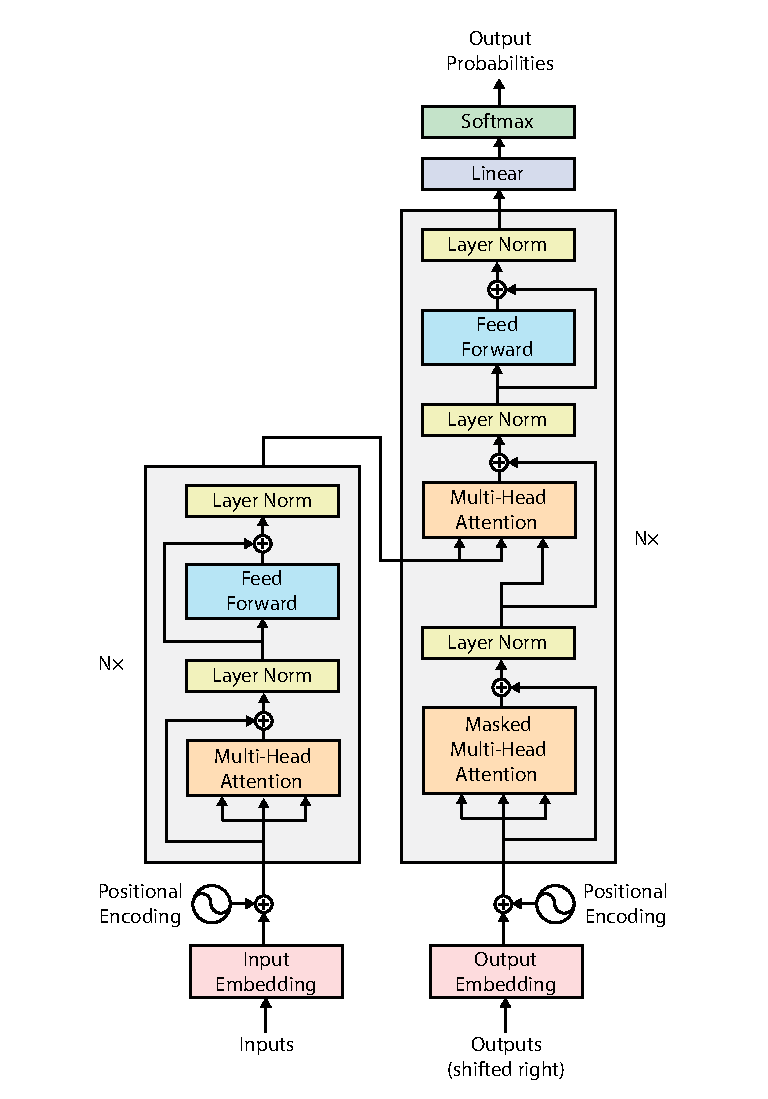
\includegraphics[width=0.8\textwidth]{figures/transformer_architecture.pdf}
    \caption{Architecture of a standard Transformer \textcite{vaswani2017attention}}
    \label{fig:transformer-architecture}
\end{figure}


\subsubsection{Tokenization}
\label{sec:tokenization}
For a Transformer to process the text input, the text is first tokenized. Tokenization is the process of breaking a sequence of text into a sequence of tokens. For example, the sentence \textit{I am a sentence.} is tokenized into the words \textit{I}, \textit{am}, \textit{a}, \textit{sentence}, and \textit{.}. The tokenization process is usually done by a tokenizer. Specifically, the transformer uses a byte pair encoding tokenizer.

\subsubsection{Embedding and Positional Encoding}
\label{sec:embedding-and-positional-encoding}
After the input text is tokenized, the next step for the model is to understand the meaning and position of the token (word) in the sequence. This is achieved by an Embedding layer and a Positional encoding layer. The results of these two layers are combined.

Two embedding layers are used. The Input Embedding layer is fed the input sequence. The Output Embedding layer accepts the target sequence after shifting the target to the right by one position and inserting a start token at the first position. The embedding layers produce a numerical representation of the input sequence, mapping each token to an embedding vector.

\begin{figure}[htp]
    \centering
    %% Creator: Matplotlib, PGF backend
%%
%% To include the figure in your LaTeX document, write
%%   \input{<filename>.pgf}
%%
%% Make sure the required packages are loaded in your preamble
%%   \usepackage{pgf}
%%
%% and, on pdftex
%%   \usepackage[utf8]{inputenc}\DeclareUnicodeCharacter{2212}{-}
%%
%% or, on luatex and xetex
%%   \usepackage{unicode-math}
%%
%% Figures using additional raster images can only be included by \input if
%% they are in the same directory as the main LaTeX file. For loading figures
%% from other directories you can use the `import` package
%%   \usepackage{import}
%%
%% and then include the figures with
%%   \import{<path to file>}{<filename>.pgf}
%%
%% Matplotlib used the following preamble
%%
\begingroup%
\makeatletter%
\begin{pgfpicture}%
\pgfpathrectangle{\pgfpointorigin}{\pgfqpoint{4.840359in}{2.401102in}}%
\pgfusepath{use as bounding box, clip}%
\begin{pgfscope}%
\pgfsetbuttcap%
\pgfsetmiterjoin%
\definecolor{currentfill}{rgb}{1.000000,1.000000,1.000000}%
\pgfsetfillcolor{currentfill}%
\pgfsetlinewidth{0.000000pt}%
\definecolor{currentstroke}{rgb}{1.000000,1.000000,1.000000}%
\pgfsetstrokecolor{currentstroke}%
\pgfsetdash{}{0pt}%
\pgfpathmoveto{\pgfqpoint{0.000000in}{-0.000000in}}%
\pgfpathlineto{\pgfqpoint{4.840359in}{-0.000000in}}%
\pgfpathlineto{\pgfqpoint{4.840359in}{2.401102in}}%
\pgfpathlineto{\pgfqpoint{0.000000in}{2.401102in}}%
\pgfpathclose%
\pgfusepath{fill}%
\end{pgfscope}%
\begin{pgfscope}%
\pgfsetbuttcap%
\pgfsetmiterjoin%
\definecolor{currentfill}{rgb}{1.000000,1.000000,1.000000}%
\pgfsetfillcolor{currentfill}%
\pgfsetlinewidth{0.000000pt}%
\definecolor{currentstroke}{rgb}{0.000000,0.000000,0.000000}%
\pgfsetstrokecolor{currentstroke}%
\pgfsetstrokeopacity{0.000000}%
\pgfsetdash{}{0pt}%
\pgfpathmoveto{\pgfqpoint{0.584568in}{0.499691in}}%
\pgfpathlineto{\pgfqpoint{4.053193in}{0.499691in}}%
\pgfpathlineto{\pgfqpoint{4.053193in}{2.252877in}}%
\pgfpathlineto{\pgfqpoint{0.584568in}{2.252877in}}%
\pgfpathclose%
\pgfusepath{fill}%
\end{pgfscope}%
\begin{pgfscope}%
\pgfsys@transformshift{0.584167in}{0.500269in}%
\pgftext[left,bottom]{\includegraphics[interpolate=true,width=3.469167in,height=1.752500in]{figures/positional_embedding-img0.png}}%
\end{pgfscope}%
\begin{pgfscope}%
\pgfsetbuttcap%
\pgfsetroundjoin%
\definecolor{currentfill}{rgb}{0.000000,0.000000,0.000000}%
\pgfsetfillcolor{currentfill}%
\pgfsetlinewidth{0.803000pt}%
\definecolor{currentstroke}{rgb}{0.000000,0.000000,0.000000}%
\pgfsetstrokecolor{currentstroke}%
\pgfsetdash{}{0pt}%
\pgfsys@defobject{currentmarker}{\pgfqpoint{0.000000in}{-0.048611in}}{\pgfqpoint{0.000000in}{0.000000in}}{%
\pgfpathmoveto{\pgfqpoint{0.000000in}{0.000000in}}%
\pgfpathlineto{\pgfqpoint{0.000000in}{-0.048611in}}%
\pgfusepath{stroke,fill}%
}%
\begin{pgfscope}%
\pgfsys@transformshift{0.584568in}{0.499691in}%
\pgfsys@useobject{currentmarker}{}%
\end{pgfscope}%
\end{pgfscope}%
\begin{pgfscope}%
\definecolor{textcolor}{rgb}{0.000000,0.000000,0.000000}%
\pgfsetstrokecolor{textcolor}%
\pgfsetfillcolor{textcolor}%
\pgftext[x=0.584568in,y=0.402469in,,top]{\color{textcolor}\rmfamily\fontsize{10.000000}{12.000000}\selectfont \(\displaystyle {0}\)}%
\end{pgfscope}%
\begin{pgfscope}%
\pgfsetbuttcap%
\pgfsetroundjoin%
\definecolor{currentfill}{rgb}{0.000000,0.000000,0.000000}%
\pgfsetfillcolor{currentfill}%
\pgfsetlinewidth{0.803000pt}%
\definecolor{currentstroke}{rgb}{0.000000,0.000000,0.000000}%
\pgfsetstrokecolor{currentstroke}%
\pgfsetdash{}{0pt}%
\pgfsys@defobject{currentmarker}{\pgfqpoint{0.000000in}{-0.048611in}}{\pgfqpoint{0.000000in}{0.000000in}}{%
\pgfpathmoveto{\pgfqpoint{0.000000in}{0.000000in}}%
\pgfpathlineto{\pgfqpoint{0.000000in}{-0.048611in}}%
\pgfusepath{stroke,fill}%
}%
\begin{pgfscope}%
\pgfsys@transformshift{1.126541in}{0.499691in}%
\pgfsys@useobject{currentmarker}{}%
\end{pgfscope}%
\end{pgfscope}%
\begin{pgfscope}%
\definecolor{textcolor}{rgb}{0.000000,0.000000,0.000000}%
\pgfsetstrokecolor{textcolor}%
\pgfsetfillcolor{textcolor}%
\pgftext[x=1.126541in,y=0.402469in,,top]{\color{textcolor}\rmfamily\fontsize{10.000000}{12.000000}\selectfont \(\displaystyle {10}\)}%
\end{pgfscope}%
\begin{pgfscope}%
\pgfsetbuttcap%
\pgfsetroundjoin%
\definecolor{currentfill}{rgb}{0.000000,0.000000,0.000000}%
\pgfsetfillcolor{currentfill}%
\pgfsetlinewidth{0.803000pt}%
\definecolor{currentstroke}{rgb}{0.000000,0.000000,0.000000}%
\pgfsetstrokecolor{currentstroke}%
\pgfsetdash{}{0pt}%
\pgfsys@defobject{currentmarker}{\pgfqpoint{0.000000in}{-0.048611in}}{\pgfqpoint{0.000000in}{0.000000in}}{%
\pgfpathmoveto{\pgfqpoint{0.000000in}{0.000000in}}%
\pgfpathlineto{\pgfqpoint{0.000000in}{-0.048611in}}%
\pgfusepath{stroke,fill}%
}%
\begin{pgfscope}%
\pgfsys@transformshift{1.668514in}{0.499691in}%
\pgfsys@useobject{currentmarker}{}%
\end{pgfscope}%
\end{pgfscope}%
\begin{pgfscope}%
\definecolor{textcolor}{rgb}{0.000000,0.000000,0.000000}%
\pgfsetstrokecolor{textcolor}%
\pgfsetfillcolor{textcolor}%
\pgftext[x=1.668514in,y=0.402469in,,top]{\color{textcolor}\rmfamily\fontsize{10.000000}{12.000000}\selectfont \(\displaystyle {20}\)}%
\end{pgfscope}%
\begin{pgfscope}%
\pgfsetbuttcap%
\pgfsetroundjoin%
\definecolor{currentfill}{rgb}{0.000000,0.000000,0.000000}%
\pgfsetfillcolor{currentfill}%
\pgfsetlinewidth{0.803000pt}%
\definecolor{currentstroke}{rgb}{0.000000,0.000000,0.000000}%
\pgfsetstrokecolor{currentstroke}%
\pgfsetdash{}{0pt}%
\pgfsys@defobject{currentmarker}{\pgfqpoint{0.000000in}{-0.048611in}}{\pgfqpoint{0.000000in}{0.000000in}}{%
\pgfpathmoveto{\pgfqpoint{0.000000in}{0.000000in}}%
\pgfpathlineto{\pgfqpoint{0.000000in}{-0.048611in}}%
\pgfusepath{stroke,fill}%
}%
\begin{pgfscope}%
\pgfsys@transformshift{2.210486in}{0.499691in}%
\pgfsys@useobject{currentmarker}{}%
\end{pgfscope}%
\end{pgfscope}%
\begin{pgfscope}%
\definecolor{textcolor}{rgb}{0.000000,0.000000,0.000000}%
\pgfsetstrokecolor{textcolor}%
\pgfsetfillcolor{textcolor}%
\pgftext[x=2.210486in,y=0.402469in,,top]{\color{textcolor}\rmfamily\fontsize{10.000000}{12.000000}\selectfont \(\displaystyle {30}\)}%
\end{pgfscope}%
\begin{pgfscope}%
\pgfsetbuttcap%
\pgfsetroundjoin%
\definecolor{currentfill}{rgb}{0.000000,0.000000,0.000000}%
\pgfsetfillcolor{currentfill}%
\pgfsetlinewidth{0.803000pt}%
\definecolor{currentstroke}{rgb}{0.000000,0.000000,0.000000}%
\pgfsetstrokecolor{currentstroke}%
\pgfsetdash{}{0pt}%
\pgfsys@defobject{currentmarker}{\pgfqpoint{0.000000in}{-0.048611in}}{\pgfqpoint{0.000000in}{0.000000in}}{%
\pgfpathmoveto{\pgfqpoint{0.000000in}{0.000000in}}%
\pgfpathlineto{\pgfqpoint{0.000000in}{-0.048611in}}%
\pgfusepath{stroke,fill}%
}%
\begin{pgfscope}%
\pgfsys@transformshift{2.752459in}{0.499691in}%
\pgfsys@useobject{currentmarker}{}%
\end{pgfscope}%
\end{pgfscope}%
\begin{pgfscope}%
\definecolor{textcolor}{rgb}{0.000000,0.000000,0.000000}%
\pgfsetstrokecolor{textcolor}%
\pgfsetfillcolor{textcolor}%
\pgftext[x=2.752459in,y=0.402469in,,top]{\color{textcolor}\rmfamily\fontsize{10.000000}{12.000000}\selectfont \(\displaystyle {40}\)}%
\end{pgfscope}%
\begin{pgfscope}%
\pgfsetbuttcap%
\pgfsetroundjoin%
\definecolor{currentfill}{rgb}{0.000000,0.000000,0.000000}%
\pgfsetfillcolor{currentfill}%
\pgfsetlinewidth{0.803000pt}%
\definecolor{currentstroke}{rgb}{0.000000,0.000000,0.000000}%
\pgfsetstrokecolor{currentstroke}%
\pgfsetdash{}{0pt}%
\pgfsys@defobject{currentmarker}{\pgfqpoint{0.000000in}{-0.048611in}}{\pgfqpoint{0.000000in}{0.000000in}}{%
\pgfpathmoveto{\pgfqpoint{0.000000in}{0.000000in}}%
\pgfpathlineto{\pgfqpoint{0.000000in}{-0.048611in}}%
\pgfusepath{stroke,fill}%
}%
\begin{pgfscope}%
\pgfsys@transformshift{3.294432in}{0.499691in}%
\pgfsys@useobject{currentmarker}{}%
\end{pgfscope}%
\end{pgfscope}%
\begin{pgfscope}%
\definecolor{textcolor}{rgb}{0.000000,0.000000,0.000000}%
\pgfsetstrokecolor{textcolor}%
\pgfsetfillcolor{textcolor}%
\pgftext[x=3.294432in,y=0.402469in,,top]{\color{textcolor}\rmfamily\fontsize{10.000000}{12.000000}\selectfont \(\displaystyle {50}\)}%
\end{pgfscope}%
\begin{pgfscope}%
\pgfsetbuttcap%
\pgfsetroundjoin%
\definecolor{currentfill}{rgb}{0.000000,0.000000,0.000000}%
\pgfsetfillcolor{currentfill}%
\pgfsetlinewidth{0.803000pt}%
\definecolor{currentstroke}{rgb}{0.000000,0.000000,0.000000}%
\pgfsetstrokecolor{currentstroke}%
\pgfsetdash{}{0pt}%
\pgfsys@defobject{currentmarker}{\pgfqpoint{0.000000in}{-0.048611in}}{\pgfqpoint{0.000000in}{0.000000in}}{%
\pgfpathmoveto{\pgfqpoint{0.000000in}{0.000000in}}%
\pgfpathlineto{\pgfqpoint{0.000000in}{-0.048611in}}%
\pgfusepath{stroke,fill}%
}%
\begin{pgfscope}%
\pgfsys@transformshift{3.836404in}{0.499691in}%
\pgfsys@useobject{currentmarker}{}%
\end{pgfscope}%
\end{pgfscope}%
\begin{pgfscope}%
\definecolor{textcolor}{rgb}{0.000000,0.000000,0.000000}%
\pgfsetstrokecolor{textcolor}%
\pgfsetfillcolor{textcolor}%
\pgftext[x=3.836404in,y=0.402469in,,top]{\color{textcolor}\rmfamily\fontsize{10.000000}{12.000000}\selectfont \(\displaystyle {60}\)}%
\end{pgfscope}%
\begin{pgfscope}%
\definecolor{textcolor}{rgb}{0.000000,0.000000,0.000000}%
\pgfsetstrokecolor{textcolor}%
\pgfsetfillcolor{textcolor}%
\pgftext[x=2.318881in,y=0.223457in,,top]{\color{textcolor}\rmfamily\fontsize{10.000000}{12.000000}\selectfont Depth}%
\end{pgfscope}%
\begin{pgfscope}%
\pgfsetbuttcap%
\pgfsetroundjoin%
\definecolor{currentfill}{rgb}{0.000000,0.000000,0.000000}%
\pgfsetfillcolor{currentfill}%
\pgfsetlinewidth{0.803000pt}%
\definecolor{currentstroke}{rgb}{0.000000,0.000000,0.000000}%
\pgfsetstrokecolor{currentstroke}%
\pgfsetdash{}{0pt}%
\pgfsys@defobject{currentmarker}{\pgfqpoint{-0.048611in}{0.000000in}}{\pgfqpoint{0.000000in}{0.000000in}}{%
\pgfpathmoveto{\pgfqpoint{0.000000in}{0.000000in}}%
\pgfpathlineto{\pgfqpoint{-0.048611in}{0.000000in}}%
\pgfusepath{stroke,fill}%
}%
\begin{pgfscope}%
\pgfsys@transformshift{0.584568in}{0.499691in}%
\pgfsys@useobject{currentmarker}{}%
\end{pgfscope}%
\end{pgfscope}%
\begin{pgfscope}%
\definecolor{textcolor}{rgb}{0.000000,0.000000,0.000000}%
\pgfsetstrokecolor{textcolor}%
\pgfsetfillcolor{textcolor}%
\pgftext[x=0.417902in, y=0.451466in, left, base]{\color{textcolor}\rmfamily\fontsize{10.000000}{12.000000}\selectfont \(\displaystyle {0}\)}%
\end{pgfscope}%
\begin{pgfscope}%
\pgfsetbuttcap%
\pgfsetroundjoin%
\definecolor{currentfill}{rgb}{0.000000,0.000000,0.000000}%
\pgfsetfillcolor{currentfill}%
\pgfsetlinewidth{0.803000pt}%
\definecolor{currentstroke}{rgb}{0.000000,0.000000,0.000000}%
\pgfsetstrokecolor{currentstroke}%
\pgfsetdash{}{0pt}%
\pgfsys@defobject{currentmarker}{\pgfqpoint{-0.048611in}{0.000000in}}{\pgfqpoint{0.000000in}{0.000000in}}{%
\pgfpathmoveto{\pgfqpoint{0.000000in}{0.000000in}}%
\pgfpathlineto{\pgfqpoint{-0.048611in}{0.000000in}}%
\pgfusepath{stroke,fill}%
}%
\begin{pgfscope}%
\pgfsys@transformshift{0.584568in}{0.842110in}%
\pgfsys@useobject{currentmarker}{}%
\end{pgfscope}%
\end{pgfscope}%
\begin{pgfscope}%
\definecolor{textcolor}{rgb}{0.000000,0.000000,0.000000}%
\pgfsetstrokecolor{textcolor}%
\pgfsetfillcolor{textcolor}%
\pgftext[x=0.279012in, y=0.793885in, left, base]{\color{textcolor}\rmfamily\fontsize{10.000000}{12.000000}\selectfont \(\displaystyle {100}\)}%
\end{pgfscope}%
\begin{pgfscope}%
\pgfsetbuttcap%
\pgfsetroundjoin%
\definecolor{currentfill}{rgb}{0.000000,0.000000,0.000000}%
\pgfsetfillcolor{currentfill}%
\pgfsetlinewidth{0.803000pt}%
\definecolor{currentstroke}{rgb}{0.000000,0.000000,0.000000}%
\pgfsetstrokecolor{currentstroke}%
\pgfsetdash{}{0pt}%
\pgfsys@defobject{currentmarker}{\pgfqpoint{-0.048611in}{0.000000in}}{\pgfqpoint{0.000000in}{0.000000in}}{%
\pgfpathmoveto{\pgfqpoint{0.000000in}{0.000000in}}%
\pgfpathlineto{\pgfqpoint{-0.048611in}{0.000000in}}%
\pgfusepath{stroke,fill}%
}%
\begin{pgfscope}%
\pgfsys@transformshift{0.584568in}{1.184529in}%
\pgfsys@useobject{currentmarker}{}%
\end{pgfscope}%
\end{pgfscope}%
\begin{pgfscope}%
\definecolor{textcolor}{rgb}{0.000000,0.000000,0.000000}%
\pgfsetstrokecolor{textcolor}%
\pgfsetfillcolor{textcolor}%
\pgftext[x=0.279012in, y=1.136304in, left, base]{\color{textcolor}\rmfamily\fontsize{10.000000}{12.000000}\selectfont \(\displaystyle {200}\)}%
\end{pgfscope}%
\begin{pgfscope}%
\pgfsetbuttcap%
\pgfsetroundjoin%
\definecolor{currentfill}{rgb}{0.000000,0.000000,0.000000}%
\pgfsetfillcolor{currentfill}%
\pgfsetlinewidth{0.803000pt}%
\definecolor{currentstroke}{rgb}{0.000000,0.000000,0.000000}%
\pgfsetstrokecolor{currentstroke}%
\pgfsetdash{}{0pt}%
\pgfsys@defobject{currentmarker}{\pgfqpoint{-0.048611in}{0.000000in}}{\pgfqpoint{0.000000in}{0.000000in}}{%
\pgfpathmoveto{\pgfqpoint{0.000000in}{0.000000in}}%
\pgfpathlineto{\pgfqpoint{-0.048611in}{0.000000in}}%
\pgfusepath{stroke,fill}%
}%
\begin{pgfscope}%
\pgfsys@transformshift{0.584568in}{1.526949in}%
\pgfsys@useobject{currentmarker}{}%
\end{pgfscope}%
\end{pgfscope}%
\begin{pgfscope}%
\definecolor{textcolor}{rgb}{0.000000,0.000000,0.000000}%
\pgfsetstrokecolor{textcolor}%
\pgfsetfillcolor{textcolor}%
\pgftext[x=0.279012in, y=1.478723in, left, base]{\color{textcolor}\rmfamily\fontsize{10.000000}{12.000000}\selectfont \(\displaystyle {300}\)}%
\end{pgfscope}%
\begin{pgfscope}%
\pgfsetbuttcap%
\pgfsetroundjoin%
\definecolor{currentfill}{rgb}{0.000000,0.000000,0.000000}%
\pgfsetfillcolor{currentfill}%
\pgfsetlinewidth{0.803000pt}%
\definecolor{currentstroke}{rgb}{0.000000,0.000000,0.000000}%
\pgfsetstrokecolor{currentstroke}%
\pgfsetdash{}{0pt}%
\pgfsys@defobject{currentmarker}{\pgfqpoint{-0.048611in}{0.000000in}}{\pgfqpoint{0.000000in}{0.000000in}}{%
\pgfpathmoveto{\pgfqpoint{0.000000in}{0.000000in}}%
\pgfpathlineto{\pgfqpoint{-0.048611in}{0.000000in}}%
\pgfusepath{stroke,fill}%
}%
\begin{pgfscope}%
\pgfsys@transformshift{0.584568in}{1.869368in}%
\pgfsys@useobject{currentmarker}{}%
\end{pgfscope}%
\end{pgfscope}%
\begin{pgfscope}%
\definecolor{textcolor}{rgb}{0.000000,0.000000,0.000000}%
\pgfsetstrokecolor{textcolor}%
\pgfsetfillcolor{textcolor}%
\pgftext[x=0.279012in, y=1.821142in, left, base]{\color{textcolor}\rmfamily\fontsize{10.000000}{12.000000}\selectfont \(\displaystyle {400}\)}%
\end{pgfscope}%
\begin{pgfscope}%
\pgfsetbuttcap%
\pgfsetroundjoin%
\definecolor{currentfill}{rgb}{0.000000,0.000000,0.000000}%
\pgfsetfillcolor{currentfill}%
\pgfsetlinewidth{0.803000pt}%
\definecolor{currentstroke}{rgb}{0.000000,0.000000,0.000000}%
\pgfsetstrokecolor{currentstroke}%
\pgfsetdash{}{0pt}%
\pgfsys@defobject{currentmarker}{\pgfqpoint{-0.048611in}{0.000000in}}{\pgfqpoint{0.000000in}{0.000000in}}{%
\pgfpathmoveto{\pgfqpoint{0.000000in}{0.000000in}}%
\pgfpathlineto{\pgfqpoint{-0.048611in}{0.000000in}}%
\pgfusepath{stroke,fill}%
}%
\begin{pgfscope}%
\pgfsys@transformshift{0.584568in}{2.211787in}%
\pgfsys@useobject{currentmarker}{}%
\end{pgfscope}%
\end{pgfscope}%
\begin{pgfscope}%
\definecolor{textcolor}{rgb}{0.000000,0.000000,0.000000}%
\pgfsetstrokecolor{textcolor}%
\pgfsetfillcolor{textcolor}%
\pgftext[x=0.279012in, y=2.163562in, left, base]{\color{textcolor}\rmfamily\fontsize{10.000000}{12.000000}\selectfont \(\displaystyle {500}\)}%
\end{pgfscope}%
\begin{pgfscope}%
\definecolor{textcolor}{rgb}{0.000000,0.000000,0.000000}%
\pgfsetstrokecolor{textcolor}%
\pgfsetfillcolor{textcolor}%
\pgftext[x=0.223457in,y=1.376284in,,bottom,rotate=90.000000]{\color{textcolor}\rmfamily\fontsize{10.000000}{12.000000}\selectfont Position}%
\end{pgfscope}%
\begin{pgfscope}%
\pgfsetrectcap%
\pgfsetmiterjoin%
\pgfsetlinewidth{0.803000pt}%
\definecolor{currentstroke}{rgb}{0.000000,0.000000,0.000000}%
\pgfsetstrokecolor{currentstroke}%
\pgfsetdash{}{0pt}%
\pgfpathmoveto{\pgfqpoint{0.584568in}{0.499691in}}%
\pgfpathlineto{\pgfqpoint{0.584568in}{2.252877in}}%
\pgfusepath{stroke}%
\end{pgfscope}%
\begin{pgfscope}%
\pgfsetrectcap%
\pgfsetmiterjoin%
\pgfsetlinewidth{0.803000pt}%
\definecolor{currentstroke}{rgb}{0.000000,0.000000,0.000000}%
\pgfsetstrokecolor{currentstroke}%
\pgfsetdash{}{0pt}%
\pgfpathmoveto{\pgfqpoint{4.053193in}{0.499691in}}%
\pgfpathlineto{\pgfqpoint{4.053193in}{2.252877in}}%
\pgfusepath{stroke}%
\end{pgfscope}%
\begin{pgfscope}%
\pgfsetrectcap%
\pgfsetmiterjoin%
\pgfsetlinewidth{0.803000pt}%
\definecolor{currentstroke}{rgb}{0.000000,0.000000,0.000000}%
\pgfsetstrokecolor{currentstroke}%
\pgfsetdash{}{0pt}%
\pgfpathmoveto{\pgfqpoint{0.584568in}{0.499691in}}%
\pgfpathlineto{\pgfqpoint{4.053193in}{0.499691in}}%
\pgfusepath{stroke}%
\end{pgfscope}%
\begin{pgfscope}%
\pgfsetrectcap%
\pgfsetmiterjoin%
\pgfsetlinewidth{0.803000pt}%
\definecolor{currentstroke}{rgb}{0.000000,0.000000,0.000000}%
\pgfsetstrokecolor{currentstroke}%
\pgfsetdash{}{0pt}%
\pgfpathmoveto{\pgfqpoint{0.584568in}{2.252877in}}%
\pgfpathlineto{\pgfqpoint{4.053193in}{2.252877in}}%
\pgfusepath{stroke}%
\end{pgfscope}%
\begin{pgfscope}%
\pgfpathrectangle{\pgfqpoint{4.269982in}{0.499691in}}{\pgfqpoint{0.087659in}{1.753186in}}%
\pgfusepath{clip}%
\pgfsetbuttcap%
\pgfsetmiterjoin%
\definecolor{currentfill}{rgb}{1.000000,1.000000,1.000000}%
\pgfsetfillcolor{currentfill}%
\pgfsetlinewidth{0.010037pt}%
\definecolor{currentstroke}{rgb}{1.000000,1.000000,1.000000}%
\pgfsetstrokecolor{currentstroke}%
\pgfsetdash{}{0pt}%
\pgfpathmoveto{\pgfqpoint{4.269982in}{0.499691in}}%
\pgfpathlineto{\pgfqpoint{4.269982in}{0.506539in}}%
\pgfpathlineto{\pgfqpoint{4.269982in}{2.246029in}}%
\pgfpathlineto{\pgfqpoint{4.269982in}{2.252877in}}%
\pgfpathlineto{\pgfqpoint{4.357642in}{2.252877in}}%
\pgfpathlineto{\pgfqpoint{4.357642in}{2.246029in}}%
\pgfpathlineto{\pgfqpoint{4.357642in}{0.506539in}}%
\pgfpathlineto{\pgfqpoint{4.357642in}{0.499691in}}%
\pgfpathclose%
\pgfusepath{stroke,fill}%
\end{pgfscope}%
\begin{pgfscope}%
\pgfsys@transformshift{4.270000in}{0.500269in}%
\pgftext[left,bottom]{\includegraphics[interpolate=true,width=0.087500in,height=1.752500in]{figures/positional_embedding-img1.png}}%
\end{pgfscope}%
\begin{pgfscope}%
\pgfsetbuttcap%
\pgfsetroundjoin%
\definecolor{currentfill}{rgb}{0.000000,0.000000,0.000000}%
\pgfsetfillcolor{currentfill}%
\pgfsetlinewidth{0.803000pt}%
\definecolor{currentstroke}{rgb}{0.000000,0.000000,0.000000}%
\pgfsetstrokecolor{currentstroke}%
\pgfsetdash{}{0pt}%
\pgfsys@defobject{currentmarker}{\pgfqpoint{0.000000in}{0.000000in}}{\pgfqpoint{0.048611in}{0.000000in}}{%
\pgfpathmoveto{\pgfqpoint{0.000000in}{0.000000in}}%
\pgfpathlineto{\pgfqpoint{0.048611in}{0.000000in}}%
\pgfusepath{stroke,fill}%
}%
\begin{pgfscope}%
\pgfsys@transformshift{4.357642in}{0.499691in}%
\pgfsys@useobject{currentmarker}{}%
\end{pgfscope}%
\end{pgfscope}%
\begin{pgfscope}%
\definecolor{textcolor}{rgb}{0.000000,0.000000,0.000000}%
\pgfsetstrokecolor{textcolor}%
\pgfsetfillcolor{textcolor}%
\pgftext[x=4.454864in, y=0.451466in, left, base]{\color{textcolor}\rmfamily\fontsize{10.000000}{12.000000}\selectfont \(\displaystyle {-1.0}\)}%
\end{pgfscope}%
\begin{pgfscope}%
\pgfsetbuttcap%
\pgfsetroundjoin%
\definecolor{currentfill}{rgb}{0.000000,0.000000,0.000000}%
\pgfsetfillcolor{currentfill}%
\pgfsetlinewidth{0.803000pt}%
\definecolor{currentstroke}{rgb}{0.000000,0.000000,0.000000}%
\pgfsetstrokecolor{currentstroke}%
\pgfsetdash{}{0pt}%
\pgfsys@defobject{currentmarker}{\pgfqpoint{0.000000in}{0.000000in}}{\pgfqpoint{0.048611in}{0.000000in}}{%
\pgfpathmoveto{\pgfqpoint{0.000000in}{0.000000in}}%
\pgfpathlineto{\pgfqpoint{0.048611in}{0.000000in}}%
\pgfusepath{stroke,fill}%
}%
\begin{pgfscope}%
\pgfsys@transformshift{4.357642in}{0.937988in}%
\pgfsys@useobject{currentmarker}{}%
\end{pgfscope}%
\end{pgfscope}%
\begin{pgfscope}%
\definecolor{textcolor}{rgb}{0.000000,0.000000,0.000000}%
\pgfsetstrokecolor{textcolor}%
\pgfsetfillcolor{textcolor}%
\pgftext[x=4.454864in, y=0.889762in, left, base]{\color{textcolor}\rmfamily\fontsize{10.000000}{12.000000}\selectfont \(\displaystyle {-0.5}\)}%
\end{pgfscope}%
\begin{pgfscope}%
\pgfsetbuttcap%
\pgfsetroundjoin%
\definecolor{currentfill}{rgb}{0.000000,0.000000,0.000000}%
\pgfsetfillcolor{currentfill}%
\pgfsetlinewidth{0.803000pt}%
\definecolor{currentstroke}{rgb}{0.000000,0.000000,0.000000}%
\pgfsetstrokecolor{currentstroke}%
\pgfsetdash{}{0pt}%
\pgfsys@defobject{currentmarker}{\pgfqpoint{0.000000in}{0.000000in}}{\pgfqpoint{0.048611in}{0.000000in}}{%
\pgfpathmoveto{\pgfqpoint{0.000000in}{0.000000in}}%
\pgfpathlineto{\pgfqpoint{0.048611in}{0.000000in}}%
\pgfusepath{stroke,fill}%
}%
\begin{pgfscope}%
\pgfsys@transformshift{4.357642in}{1.376284in}%
\pgfsys@useobject{currentmarker}{}%
\end{pgfscope}%
\end{pgfscope}%
\begin{pgfscope}%
\definecolor{textcolor}{rgb}{0.000000,0.000000,0.000000}%
\pgfsetstrokecolor{textcolor}%
\pgfsetfillcolor{textcolor}%
\pgftext[x=4.454864in, y=1.328059in, left, base]{\color{textcolor}\rmfamily\fontsize{10.000000}{12.000000}\selectfont \(\displaystyle {0.0}\)}%
\end{pgfscope}%
\begin{pgfscope}%
\pgfsetbuttcap%
\pgfsetroundjoin%
\definecolor{currentfill}{rgb}{0.000000,0.000000,0.000000}%
\pgfsetfillcolor{currentfill}%
\pgfsetlinewidth{0.803000pt}%
\definecolor{currentstroke}{rgb}{0.000000,0.000000,0.000000}%
\pgfsetstrokecolor{currentstroke}%
\pgfsetdash{}{0pt}%
\pgfsys@defobject{currentmarker}{\pgfqpoint{0.000000in}{0.000000in}}{\pgfqpoint{0.048611in}{0.000000in}}{%
\pgfpathmoveto{\pgfqpoint{0.000000in}{0.000000in}}%
\pgfpathlineto{\pgfqpoint{0.048611in}{0.000000in}}%
\pgfusepath{stroke,fill}%
}%
\begin{pgfscope}%
\pgfsys@transformshift{4.357642in}{1.814581in}%
\pgfsys@useobject{currentmarker}{}%
\end{pgfscope}%
\end{pgfscope}%
\begin{pgfscope}%
\definecolor{textcolor}{rgb}{0.000000,0.000000,0.000000}%
\pgfsetstrokecolor{textcolor}%
\pgfsetfillcolor{textcolor}%
\pgftext[x=4.454864in, y=1.766355in, left, base]{\color{textcolor}\rmfamily\fontsize{10.000000}{12.000000}\selectfont \(\displaystyle {0.5}\)}%
\end{pgfscope}%
\begin{pgfscope}%
\pgfsetbuttcap%
\pgfsetroundjoin%
\definecolor{currentfill}{rgb}{0.000000,0.000000,0.000000}%
\pgfsetfillcolor{currentfill}%
\pgfsetlinewidth{0.803000pt}%
\definecolor{currentstroke}{rgb}{0.000000,0.000000,0.000000}%
\pgfsetstrokecolor{currentstroke}%
\pgfsetdash{}{0pt}%
\pgfsys@defobject{currentmarker}{\pgfqpoint{0.000000in}{0.000000in}}{\pgfqpoint{0.048611in}{0.000000in}}{%
\pgfpathmoveto{\pgfqpoint{0.000000in}{0.000000in}}%
\pgfpathlineto{\pgfqpoint{0.048611in}{0.000000in}}%
\pgfusepath{stroke,fill}%
}%
\begin{pgfscope}%
\pgfsys@transformshift{4.357642in}{2.252877in}%
\pgfsys@useobject{currentmarker}{}%
\end{pgfscope}%
\end{pgfscope}%
\begin{pgfscope}%
\definecolor{textcolor}{rgb}{0.000000,0.000000,0.000000}%
\pgfsetstrokecolor{textcolor}%
\pgfsetfillcolor{textcolor}%
\pgftext[x=4.454864in, y=2.204652in, left, base]{\color{textcolor}\rmfamily\fontsize{10.000000}{12.000000}\selectfont \(\displaystyle {1.0}\)}%
\end{pgfscope}%
\begin{pgfscope}%
\pgfsetbuttcap%
\pgfsetmiterjoin%
\pgfsetlinewidth{0.803000pt}%
\definecolor{currentstroke}{rgb}{0.000000,0.000000,0.000000}%
\pgfsetstrokecolor{currentstroke}%
\pgfsetdash{}{0pt}%
\pgfpathmoveto{\pgfqpoint{4.269982in}{0.499691in}}%
\pgfpathlineto{\pgfqpoint{4.269982in}{0.506539in}}%
\pgfpathlineto{\pgfqpoint{4.269982in}{2.246029in}}%
\pgfpathlineto{\pgfqpoint{4.269982in}{2.252877in}}%
\pgfpathlineto{\pgfqpoint{4.357642in}{2.252877in}}%
\pgfpathlineto{\pgfqpoint{4.357642in}{2.246029in}}%
\pgfpathlineto{\pgfqpoint{4.357642in}{0.506539in}}%
\pgfpathlineto{\pgfqpoint{4.357642in}{0.499691in}}%
\pgfpathclose%
\pgfusepath{stroke}%
\end{pgfscope}%
\end{pgfpicture}%
\makeatother%
\endgroup%

    \caption{The 64-dimensional positional encoding for a sentence with the maximum length of 512. Each row represents the embedding vector p\_t}
\end{figure}

\todo{Rewrite}
The positional encoding is generated by a sinusoidal positional encoding layer. This layer is fed the sequence length and produces a sinusoidal positional encoding vector. The positional encoding vector is then added to the embedding vector.

\subsubsection{Encoder and decoder stacks}
\label{sec:encoder-decoder-stacks}
A Transformer is comprised of two main parts: the encoder and the decoder. The encoder is responsible for encoding the input sequence into a sequence of vectors. It tries to capture information about which parts of the inputs are relevant to each other. The decoder is responsible for decoding the output sequence from the encoder. Along with other inputs, the decoder is optimized for generating outputs. In \cref{fig:transformer-architecture}, the left and right halves represent the Transformer encoder and decoder, respectively. 

The encoder and decoder are both composed of a stack of self-attention layers. This layer allows the model to pay more or less attention to certain words in the input sentence as it is handling a specific word. Each decoder layer has an additional attention mechanism that draws information from the outputs of previous decoders, before the decoder layer draws information from the encodings. Both the encoder and decoder layers contain a feed-forward layer for further processing of the outputs, as well as layer normalization and residual connections.

The transformer architecture allows for auto-regressive text generation. This is achieved by re-feeding the decoder the encoder outputs. The decoder then generates the next word in a loop until the end of the sentence is reached. For this to work, the  Transformer must not be able to use the current or future output to predict an output. The use of a look-ahead mask solves this. The final output from the transformer is generated by feeding the decoder output through a linear layer and a softmax layer. This produces probabilities for each token in the vocabulary and can be used to predict the next token (word).

The encoder and decoder can also be used independently or in combination. The original transformer model described by \textcite{vaswani2017attention} used an encoder-decoder structure. These models are used for generative tasks that also require input, for example, language translation or text summarization. Encoder-only models are used for tasks that are centered around understanding the input, such as sentence classification and named entity recognition. Decoder-only models excel at generative tasks such as text generation.

\begin{figure}[htp]
    \centering
    \begin{subfigure}[b]{0.5\textwidth}
        \centering
        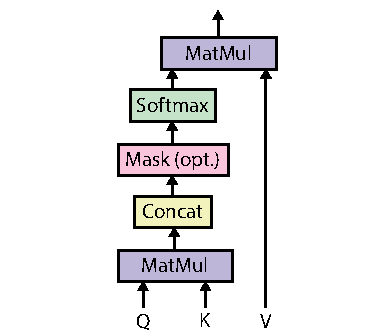
\includegraphics[width=0.8\textwidth,keepaspectratio]{figures/scaled_dot-product_attention.pdf}
        \caption{Scaled Dot-Product Attention.}
        \label{fig:scaled-dotproduct-attention}
    \end{subfigure}%
    \hfill
    \begin{subfigure}[b]{0.5\textwidth}
        \centering
        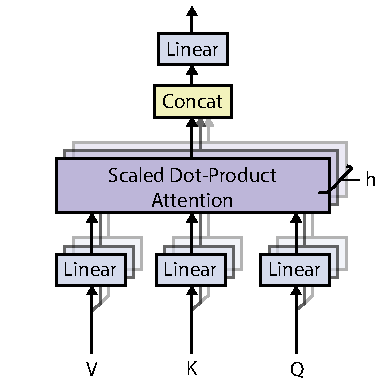
\includegraphics[width=0.8\textwidth,keepaspectratio]{figures/multi-head_attention.pdf}
        \caption{Multi-Head Attention consists of several attention layers running in parallel.}
        \label{fig:multihead-attention}
    \end{subfigure}%
    \caption{Multi-Head Attention module in Transformer architecture \textcite{vaswani2017attention}}
    \label{fig:transformer-architecture-details}
\end{figure}

\subsubsection{Scaled dot-product attention} 
\label{sec:scaled-dot-product-attention}
The self-attention layer used in each Transformer block is named "Scaled Dot-Product Attention". An overview of the attention layer is shown in \cref{fig:scaled-dotproduct-attention}. The layer learns three weight matrices, query weights \(W_Q\), key weights \(W_K\), and value weights \(W_V\). Each input word embedding is multiplied with each weight matrix, producing a query vector, key vector, and value vector. Self-attention scores are then generated by calculating the dot products of the query vector with the key vector of the respective word (query) that is calculated.

In order to stabilize the gradients during training, the attention weights are divided by the square root of the dimension of the key vectors, \(\sqrt{d_{k}}\). A softmax function is then applied, normalizing the scores to be positive and adding up to 1. Each value vector is then multiplied by the the softmax score. The resulting weighted value vectors are then summed up and serve as output from the attention layer.

In practice, the attention calculation for all tokens can be expressed as one large matrix calculation. This significantly speeds up the training process. The queries, keys, and values are packed into separate matrices. The output matrix can be described as:
\todo{T means transpose. Since this is matrix calculations, do I need to add an explanation of this?}
\begin{equation}
    \text{Attention$(Q,K,V)$} = \text{softmax}(\frac{QK^T}{\sqrt{d_{k}}})V
\end{equation}


\subsubsection{Multi-head attention}
\label{sec:multi-head-attention}
By splitting the query, key, and value parameters in N-ways (logically), each with its separate weight matrix, the performance of the Transformer is increased. This is called multi-head attention, illustrated in \cref{fig:multihead-attention}. It gives the Transformer greater power to encode multiple relationships and nuances for each word. The final attention outputs for the feed-forward network are calculated by concatenating the matrixes for each attention head.

\subsection{Training}
\label{sec:transformer-training}
A Transformer model typically undergoes something called self-supervised learning. This is an intermediary between both unsupervised- and supervised learning. This normally conforms to unsupervised pre-training the model on a large set of data. Then, the model is fine-tuned on a (usually) smaller dataset of labeled data.

In contrast to the unsupervised training, where the target sequence comprises the predicted transformer output, the supervised training is done by feeding the complete input- and target language sequence directly into the Transformer. The input sequence is fed to the encoder, while the target sequence is fed to the decoder.

\subsection{Inference}
\label{sec:transformer-inference}
For making inference, the Transformer is only fed the input sequence. The encoder is run on the input sequence, and the encoder output is fed to the decoder. Since no encoder output is available at the first timestep, the decoder is fed a special "<start>" token. The decoder output is then fed back into the decoder again. This process is repeated until the decoder output encounters a special "<stop>" token.

\todo{More concrete example to explain this. Maybe a figure?}

\section{Metrics}
\label{sec:metrics}

\subsection{Performance metric}
\label{sec:performance-metric}

\subsubsection{Accuracy}
\label{sec:accuracy}

\subsubsection{Perplexity}
\label{sec:perplexity}

\subsection{Machine translation metrics}
\label{sec:machine-translation-metrics}

\subsubsection{\textsc{Bleu}}
\label{sec:blue-score}
\acrfullr{bleu} by \textcite{papineni2002bleu} is a metric for automatically evaluating machine-translated text. \acrshort{bleu} scores are between 0 and 1. A value of 0 means there is no overlap with the reference translation, while a value of 1 means that the translation perfectly overlaps. A score of 0.6 or 0.7 is considered the best you can achieve. The method is based on n-gram matching, where n-grams in the reference translation are matched against n-grams in the translation. The matches are position-independent. The more matches, the higher the score.\\

\noindent For example, consider the following two translations:\\

\indent Candidate: \underline{on} \underline{the} \underline{mat} \underline{the} \underline{cat} sat.\\
\indent Reference: \underline{The} \underline{cat} is \underline{on} \underline{the} \underline{mat}.\\

\noindent The unigram precision \(\left(p_1\right) = 5/6\)\\

\noindent However, machine translations tend to generate an abundance of reasonable words, which could result in an inaccurately high precision. To combat this, \acrshort{bleu} uses something called modified precision. The modification consists of clipping the occurrence of an n-gram to the maximum number the n-gram occurs in the reference. These clipped precision scores \(\left(p_n\right)\) are then calculated for n-grams up to length \(N\), normally 1-grams through 4-grams. They are then combined by computing the geometric average precision. In addition, positive weights \(w_n\) are used, normally set to \(w_n = 1/N\).

\begin{equation}
    \label{eq:geometric-average-precision}
    \text{Geometric Average Precision $\left(N\right)$} = \exp \left( \sum_{n=1}^{N} w_n \log{p_n} \right)
\end{equation}

\noindent \acrshort{bleu} also introduces a brevity penalty for penalizing translations that are shorter than the reference.

\begin{equation}
    \label{eqn:brevity-penalty}
    \text{Brevity Penalty} = 
    \begin{cases}
        1 & \text{if } c > r\\
        e^{\left(1-r/c \right)} & \text{if } c \le r
    \end{cases}
\end{equation}

\noindent The final \acrshort{bleu} score is then computed as:

\begin{equation}
    \label{eqn:bleu}
    \textsc{Bleu} = \text{Brevity Penalty} \cdot \text{Geometric Average Precision Scores $\left(N\right)$}
\end{equation}

\subsection{String metric}
\label{sec:string-metric}

\subsubsection{Jaccard index}
\label{sec:jaccard-index}
TODO: Used for smart contract filtering

\section{Blockchain}
\label{sec:blockchain}
The blockchain technology was popularized by Bitcoin in 2008. Satoshi Nakamoto introduced the formal idea of blockchain as a peer-to-peer electronic cash system. It enabled users to conduct transactions without the need for a central authority. A blockchain is a growing list of records that are linked together by a cryptographic hash. Each record is called a block. The blocks contain a cryptographic hash of the previous block, a timestamp, and transactional data. By time-stamping a block, this proves that the transaction data existed when the block was published in order to get into its hash. Since all blocks contains the hash of the previous block, they end up forming a chain. In order to tamper with a block in the chain, this also requires altering all subsequent blocks. Blockchains are therefore resistant to modification. The longer the chain, the more secure it is.

Typically, blockchains are managed by a peer-to-peer network, resulting in a publicly distributed ledger. The network is composed of nodes that are connected to each other. The nodes collectively adhere to a protocol in order to communicate and validate new blocks. Blockchain records are possible to alter through a \gls{fork}. However, blockchains can be considered secure by design and present a distributed computing system with high Byzantine fault tolerance \cite{sankar2017survey}.

From Bitcoin sprang several other cryptocurrencies and blockchain platforms such as Ethereum, Litescoin, and Ripple. \cref{tab:blockchain-platforms} shows an overview of the different blockchain platforms, including the different consensus protocols, programming languages, and execution environments used. It also shows the different types of blockchains, including public, private, and hybrid.


\subsection{Ethereum blockchain}
\label{sec:ethereum}


\section{Smart Contract}
\label{sec:smart-contract}
\todo{Rewrite and adapt to vulnerabilities SoliDetector can detect.}

The term "\acrlong{sc}" was introduced with the Ethereum platform in 2014. A \acrfull{sc} is a program that is executed on a blockchain, enabling non-trusting parties to create an \textit{agreement}. \acrshortpl{sc} have enabled several interesting new concepts, such as \acrfull{nft} and entirely new business models. Since Ethereum's introduction of \acrshortpl{sc}, the platform has kept its market share as the most popular \acrshort{sc} blockchain platform. Ethereum is a open, decentralized platform that allows users to create, store, and transfer digital assets. Solidity is a programming language that is used to write smart contracts in Ethereum. Solidity is compiled down to bytecode, which is then deployed and stored on the blockchain. Ethereum also introduces the concept of gas. Ethereum describes gas as follows: \textquote{It is the fuel that allows it to operate, in the same way that a car needs gasoline to run.} \cite{ethereum2021gas}. The gas is used to pay for the cost of running the smart contract. This protects against malicious actors spamming the network \cite{ethereum2021gas}. The gas is paid in Wei, which is the smallest unit of Ethereum. Due to the immutable nature of blockchain technology, once a smart contract is deployed, it cannot be changed. This can have serious security implications, as vulnerable contracts can not be updated.

\subsection{Security Vulnerabilities}
\label{sec:smart-contract-vulnerabilities}
There are many vulnerabilities in \acrfullpl{sc} that can be exploited by malicious actors. Throughout the last years, an increase in the use of the Ethereum network has led to the development of \acrshortpl{sc} that are vulnerable to attacks. Due to the nature of blockchain technology, the attack surface of \acrshortpl{sc} is somewhat different from that of traditional computing systems. The Smart Contract Weakness Classification (SWC) Registry \footnote{\url{https://swcregistry.io}} collects information about various vulnerabilities. Following is a list of the most common vulnerabilities in \acrlongpl{sc}:

\subsubsection{Integer Overflow and Underflow}
Integer overflow and underflows happen when an arithmetic operation reaches the maximum or minimum size of a certain data type. In particular, multiplying or adding two integers may result in a value that is unexpectedly small, and subtracting from a small integer may cause a wrap to be an unexpectedly large positive value. For example, an 8-bit integer addition 255 + 2 might result in 1.

\subsubsection{Transaction-Ordering Dependence}
In blockchain systems, there is no guarantee on the execution order of transactions. A miner can influence the outcome of a transaction due to its own reordering criteria. For example, a transaction that is dependent on another transaction to be executed first may not be executed. This can be exploited by malicious actors. 

\subsubsection{Broken Access Control}
Access Control issues are common in most systems, not just smart contracts. However, due to the monetary nature and openness of most \acrshortpl{sc}, properly enforcing access controls are essential. Broken access control can, for example, occur due to wrong visibility settings, giving attackers a relatively straightforward way to access contracts' private assets. However, the bypass methods are sometimes more subtle. For example, in Solidity, reckless use of \lstinline[language=Solidity]!delegatecall! in proxy libraries, or the use of the deprecated \lstinline[language=Solidity]!tx.origin! might result in broken access control. \cref{lst:broken-access-control} shows a simple Solidity contract where anyone is able to trigger the contract's self-destruct, which makes the code vulnerable.

\begin{lstlisting}[
    caption={Access control vulnerable Solidity \acrlong{sc} code},
    label=lst:broken-access-control,
    language=Solidity]s
contract SimpleSuicide {
    function sudicideAnyone() {
        selfdestruct(msg.sender);
    }
}
\end{lstlisting}

\subsubsection{Timestamp Dependency}
If a \acrlong{sc} is dependent on the timestamp of a transaction, it is vulnerable to attacks. A miner has control over the execution environment for the executing \acrshort{sc}. If the \acrshort{sc} platform allows for \acrshortpl{sc} to use the time defined by the execution environment, this can result in a vulnerability. An example vulnerable use is a timestamp used as part of the conditions to perform a critical operation (e.g., sending ether) or as the source of entropy to generate random numbers. Hence, if the miner holds a stake in a contract, he could gain an advantage by choosing a suitable timestamp for a block he is mining. \cref{lst:timestamp-dependency} shows an example Solidity \acrshort{sc} code that contains this vulnerability. Here, the timestamp (the \lstinline[language=Solidity]!now! keyword on line 10) is used as a source of entropy to generate a random number.

\begin{lstlisting}[
    caption={Timestamp Dependency vulnerable Solidity \acrlong{sc} code},
    label=lst:timestamp-dependency,
    language=Solidity]
contract Roulette {
    uint public prevBlockTime; // One bet per block
    constructor() external payable {} // Initially fund contract
    
    // Fallback function used to make a bet
    function () external payable {
        require(msg.value == 5 ether); // Require 5 ether to play
        require(now != prevBlockTime); // Only 1 transaction per block
        prevBlockTime = now;
        if(now % 15 == 0) { // winner
            msg.sender.transfer(this.balance);
        }
    }
}
\end{lstlisting}

\subsubsection{Reentrancy}
Reentrancy is a vulnerability that occurs when a \acrshort{sc} calls external contracts. Most blockchain platforms that implement \acrshort{sc} provide a way to make external contract calls. In Ethereum, an attacker may carefully construct a \acrshort{sc} at an external address that contains malicious code in its fallback function. Then, when a contract sends funds to the address, it will invoke the malicious code. Usually, the malicious code triggers a function in the vulnerable contract, performing operations not expected by the developer. It is called "reentrancy" since the external malicious contract calls a function on the vulnerable contract and the code execution then "reenters" it. \cref{lst:reentrancy} shows a Solidity \acrshort{sc} function where a user is able to withdraw all the user's funds from a contract. If a malicious actor carefully crafts a contract that calls the withdrawal function several times before completing, the actor would successfully withdraw more funds than the current available balance. This vulnerability could be eliminated by updating the balance (line 4) before transferring the funds (line 3).

\begin{lstlisting}[
    caption={Reentrancy vulnerable Solidity \acrlong{sc} code},
    label=lst:reentrancy,
    language=Solidity]
function withdraw() external {
    uint256 amount = balances[msg.sender];
    require(msg.sender.call.value(amount)());
    balances[msg.sender] = 0;
}   
\end{lstlisting}



\section{Vulnerability detection}
\label{sec:vulnerability-detection}
\todo{Condence into one section, describing the different methods.. Add ontology based detection (for SoliDetector)}
Many tools and methods for vulnerability detection have been developed over recent years. This includes both static and dynamic vulnerability techniques, as well as tools based on \acrfull{ml}. These tools can be categorized in terms of their primary function. This includes symbolic execution, syntax analysis, abstract interpretation, data flow analysis, fuzzy testing, and machine learning. In the following sections, the identified vulnerability detection tools are summarized, compared, and analyzed in detail.

\subsection{Symbolic execution}
\label{sec:symbolic-execution}
Symbolic execution is a method for analyzing a computer program in order to determine what inputs cause each part of a program to execute. Symbolic execution requires the program to run. During the execution of the program, symbolic values are used instead of concrete values. The program execution arrives at expressions in terms of symbols for expressions and variables, as well as constraints expressed as symbols for each possible outcome of each conditional branch of the program. Finally, the possible inputs, expressed as symbols, that trigger a branch can be determined by solving the constraints.

\subsubsection{Syntax analysis}
\label{sec:syntax-analysis}
Syntax analysis is a technique for analyzing computer programs by analyzing the syntactical features of a computer program. This usually involves some kind of pattern matching where the source code is first parsed into a tree structure. This tree is then analyzed by looking for vulnerable patterns while traversing the tree.

\subsubsection{Abstract interpretation}
\label{sec:abstract-interpretation}
Abstract interpretation is a method to analyze computer programs by soundly approximating the semantics of a computer program. This results in a superset of the concrete program semantics. Normally, this is then used to automatically extract information about the possible executions of computer programs.

\subsubsection{Data flow analysis}
\label{sec:data-flow-analysis}
Data flow analysis is a method for analyzing computer programs by gathering information about the flow of data through the source code. This is done by collecting all the possible set of values calculated at different points through a computer program. This method is able to analyze large programs, compared to, for example, symbolic execution.

\subsubsection{Fuzzy testing}
\label{sec:fuzzy-testing}
Fuzzing is an automated testing technique for analyzing computer programs. The technique involves supplying invalid, unexpected, or random data inputs to a program in order to uncover bugs. The program is then monitored during execution for unexpected behavior such as crashes, errors, or failing built-in code assertions.

\chapter{Related work}
\label{chap:related-work}

This chapter presents related research in the field of source code synthesis. \cref{sec:code-synthesis} presents various techniques for code synthesis. The section begins with presenting some of the earlier techniques, followed by surveying more recent and state-of-the-art code synthesis techniques. In \cref{sec:bias-in-language-models} works related to bias in language models are presented.

%\section{Language models}
%\label{sec:language-models}
%The problem of generating code is fundamentally a language modeling problem. Language modeling is the task of predicting the next word in a text given the previous words. This section begins with presenting some of the earlier techniques, followed by surveying more recent and state-of-the-art language models.
%
%
%The first few language models came in the form of n-grams, a term first referenced by \textcite{shannon1948ngram}. An n-gram is a %contiguous sequence of n items from a given sample of text. Most early approaches employed n-grams with smoothing to handle unseen %n-grams \textcite{kneser1995improved}.
%
%\subsection{Non-context models}
%\subsection{Context aware models}
%\subsection{Word embeddings}
%Tomas Mikolov's Word2vec (google team),
%Stanford University's GloVe
%GN-GloVe (genderneutral) ->point tto thte bias problem off datasets -> link to insecure code on  github
%
%\subsection{Neural language models}
%N-grams
%
%CoVe (Contextualized Word Vectors) needs "fixed" prettrained dataset :: Learned in Translation: Contextualized Word Vectors
%
%ELMo biLM
%
%Universal Language Model Fine-tuning (ULMFiT) :: introduced the concept of fine-tuning the language model.
%
%OpenAI’s Gener- ative Pre-training Transformer (GPT)
%
%GPT-2, improved version of GPT. Works without fine-tuning. (concerns of it being used to generate unintended or malicious content - %delayed release)
%
%Bidirectional Encoder Representations from Transformers (BERT) - > bidirectttional, in comparison to GPT
%
%BERT is a bimodal Transformer with 12 layers, 768 dimentional hidden states, and 12 attention heads.
%
%-----
%GPT-3 (Codex)
%
%GPT-J (Opensoursed)
%
%
\section{Code synthesis}
\label{sec:code-synthesis}
Code synthesis is the task of generating code from a given specification. One of the earlier classical works used a probabilistic \acrfull{pcfg} \cite{allamanis2015bimodal}. \textcite{hindle2012natural} investigated whether code could be modeled by statistical language models. In particular, the authors used an n-gram model. They argue that "programs that real people actually write are mostly simple and rather repetitive, and thus they have usefully predictable statistical properties". They found that code is more predictable than natural languages. DeepCoder by \textcite{balog2017deepcoder} focused on solving programming competition-style problems. They trained a neural network for predicting properties of source code, which could be used for guiding program search.

\subsection{Code synthesis based on code semantics}
Programs can also be synthesized by leveraging the semantics of the code. \textcite{alon2018code2vec} purposes a tool named code2vec. It is a neural network model for representing snippets of code as continuously distributed vectors, or "code embeddings". The authors leverage the semantic structure of code by passing serialized \acrfullpl{ast} into a neural network. Code2seq \cite{alon2018code2seq} builds on the works of \textcite{alon2018code2vec} which focuses on natural language sequence generation from code snippets. The authors use an encoder-decoder LSTM model and rely on \acrshortpl{ast} for code snippets. The model is trained on three Java corpuses small, medium, and large, achieving a \gls{f1} score of 50.64, 53.23, and 59.19, respectively. However, the model is limited to only considering the immediately surrounding context. Pythia by \textcite{svyatkovskiy2019pyhia} is able to generate ranked lists of method and API recommendations to be used by software developers at edit time. The code completion system is based on \acrshortpl{ast} and uses Word2vec for producing code embeddings of Python code. These code embeddings are then used to train a \gls{lstm} model. The model is evaluated on a dataset of 15.8 million method calls extracted from real-world source code, achieving an accuracy of 92\%.

\subsection{Code synthesis based on transformers}
\label{sec:transformers-for-code-synthesis}
Inspired by the success of large natural language models such as \acrfullr{elmo} \cite{peters2018deep}, \acrfullr{gpt} \cite{radford2018improving}, \acrfullr{bert} \cite{devlin2018bert}, XLNet \cite{yang2019xlnet}, and RoBERTa \cite{liu2019roberta}, large-scale Transformer models have been applied in the domains of code synthesis. \textcite{feng2020codebert} proposes a new approach to code synthesis by training the BERT transformer model on Python \gls{docstring} paired with functions. The resulting 125M parameter transformer model, named CodeBERT \cite{feng2020codebert}, achieves strong results on code-search and code-to-text generation. The authors also observe that models that leverage code semantics (\acrshortpl{ast}) can produce slightly better results. PyMT5 \textcite{colin2020pymt5} is based on the T5 model. The model can predict whole methods from natural language documentation strings (docstrings) and summarize code into docstrings of any common style. For method generation, PyMT5 achieves a \gls{bleu} score of 0.0859 and a F-score of 24.8 on the CodeSearchNet \cite{codesearchnet} test set. GPT-C by \textcite{svyatkovskiy2020intellicode} is a model based on GPT-2. The 366M parameter-sized model is trained on a code corpus consisting of 1.2 billion lines of source code in Python, C\#, JavaScript and TypeScript programming languages. The Python-only model reportedly achieves a ROUGE-L precision of 0.80 and recall of 0.86.

The model complexity of transformers has recently sky-rocketed, with model sizes growing to several tens of billions of parameters. GPT-J is a 6 billion parameter model trained on The Pile, which is an 825GB dataset. The pre-trained version of GPT-J is also publicly available. Codex by \textcite{chen2021codex} is a 12 billion parameter model based on GPT. It was trained on 54 million GitHub repositories, and a production version of Codex powers GitHub Copilot \cite{copilot}. The model solves 28.8\% of the problems in the HumanEval dataset \cite{chen2021codex}, while GPT-3 solves 0\% and GPT-J solves 11.4\%. Google DeepMind's AlphaCode \cite{alphacode} is 41.4 billion parameters and is the first AI to reach a competitive level in programming competitions. AlphaCode was tested against challenges curated by Codeforces \cite{codeforces}, a competitive coding platform. It achieved an average ranking of 54.3\% across 10 contests. The authors found that repeated sampling on the same problem significantly increased the probability of a correct solution.


\newcommand*\emptycirc[1][1ex]{\tikz\draw (0,0) circle (#1);} 
\newcommand*\halfcirc[1][1ex]{%
  \begin{tikzpicture}
  \draw[fill] (0,0)-- (90:#1) arc (90:270:#1) -- cycle ;
  \draw (0,0) circle (#1);
  \end{tikzpicture}}
\newcommand*\fullcirc[1][1ex]{\tikz\fill (0,0) circle (#1);} 


%\begin{sidewaystable}
\begin{ThreePartTable}
    \newcolumntype{Y}{>{\centering\arraybackslash}X}
    \newcolumntype{R}{>{\raggedright\arraybackslash}X}
    \def\arraystretch{1.5}
    \setlength\tabcolsep{6pt} % <--- important, (default 6pt)
    \setlength{\LTleft}{-20cm plus -1fill}
    \setlength{\LTright}{\LTleft}
    \footnotesize
    \begin{center}
    \keepXColumns
    \begin{tabularx}{1\textwidth}{clRRRRR}
            \caption{Existing language models.}\label{tab:code-synthesis-models}\\
            \toprule
            \textbf{Refs.} & \textbf{Year} & \textbf{Model} & \textbf{Metrics} & \textbf{Languages} &  \textbf{Input} & \textbf{Output}\\
            \hline
            \endfirsthead
            \caption{(\textit{Continued}) Existing static smart contract vulnerability detection tools.}\\
            \toprule
            \textbf{Refs.} & \textbf{Year} & \textbf{Model} & \textbf{Metrics} & \textbf{Languages} &  \textbf{Input} & \textbf{Output}\\
            \hline
        \endhead
            \midrule
            \multicolumn{7}{r}{\small(\textit{Continued on next page})}\\
        \endfoot
        \endlastfoot
        
        \cite{feng2020codebert} & \citeyear{feng2020codebert} & CodeBERT & \acrshort{bleu} & Python  & Code & Docstring\\
        \cite{colin2020pymt5} & \citeyear{colin2020pymt5} & PyMT5 & \acrshort{bleu} & Python & Docstring & Code\\
        \cite{svyatkovskiy2020intellicode} & \citeyear{svyatkovskiy2020intellicode} & GPT-C & ROUGE-L & Python, C\#, JavaScript, TypeScript &  & \\
        \cite{chen2021codex} & \citeyear{chen2021codex} & Codex & Functional correctness & Python & Docstring & Code\\
        \cite{alphacode} & \citeyear{alphacode} & AlphaCode & Functional correctness & Python, C++, Java & Problem  description & Code\\
        \bottomrule
    \end{tabularx}
    \end{center}

\end{ThreePartTable}
%\end{sidewaystable}

As can be seen from \cref{tab:code-synthesis-models}, most of the models are concerned with Python code. However, none have attempted to generate \acrfullpl{sc} code. \acrshort{sc} code is quite different from most of the other popular languages such as Python, JavaScript, and Java. Investigating how transformer models perform on \acrshort{sc} code would give valuable insight into the future of code synthesis. Further, all of the works listed in \cref{tab:code-synthesis-models} that are concerned with text-to-code generation, only consider using comments in isolation. There is therefore a need for an investigation of a code generation approach that uses both comments and code for generating functions.

\section{Bias in language models}
\label{sec:bias-in-language-models}
One of the main problems with language models is that they often contain bias \cite{li2021detecting}. This can be everything from producing gender-specific jobs to favoring a certain race. There have been several works related to mitigating this in language models. However, with varying success. \textcite{Silva2021TowardsAC} tried to mitigate societal bias in text generation using a loss regularizer to “de-bias” a RoBERTa model. However, their approach was not successful and conclude there is a need for more robust bias testing in transformers. Several works are devoted to using adversarial methods to reduce bias. \textcite{laftr2018} propose LAFTER, an adversarial method to modify the training objective based on a desired fairness measure. \textcite{zhang2018mitigating} also tries to reduce bias using adversarial training. However, \cite{zhang2018mitigating} states that the adversarial training method is hard to get right and is often touchy. \textcite{mitigating2021} investigates bias in visual transformer models, as they find existing approaches such as LAFTR unable to maintain high performance. They propose TADeT, a targeted alignment strategy for debasing transformers that aims to discover and remove bias primarily from query matrix features. 

In the area of code synthesis, vulnerabilities can be considered a form of bias in language models. However, there seems to be very little research on the security of synthesized code using transformers. \cite{chen2021codex} provide a brief discussion of insecure code generated by Codex. However, this investigation was limited to the exploration of the generation of cryptographic functions. \textcite{pearch2021asleep} acknowledge this gap in research and conduct a vulnerability analysis of GitHub Copilot (based on Codex). They construct a manual dataset of incomplete python and C code that \textit{may} produce a vulnerability. From their analysis of 1689 synthesized Python and C programs, they conclude with approximately 40\% are vulnerable. This shows there is a dire need for reducing the number of vulnerabilities generated with language models.


% vvvvvvvv VIKTIG vvvvvvvvvv

%autoregressive generation tasks
%see https://arxiv.org/pdf/2005.08025.pdf for structuring thesisl....!!!!

%see docstring analysis 2.3 of https://arxiv.org/pdf/2010.03150.pdf for clustering comments....
%^^^^^^^^ VIKTIG ^^^^^^^^


%\todo{Try to find papers that reviewe style of comments}
%Several papers on generating code comments from source code are available. The following is a list of the most popular papers.

%However, to the best of my knowledge, there is no paper investigating how to best write comments for auto-generating code. There are however, 




\chapter{Research Methodology}
\label{chap:research-methodoloy}
This chapter presents the research methodology used in this thesis. Firstly, the research motivation is presented in \cref{sec:research-motivation}, followed by the research questions defined for this thesis in \cref{sec:research-questions}. The research method and design are explained in \cref{sec:research-method-and-design}. Then, \cref{sec:design-for-rq1,sec:design-for-rq2} presents the research design for RQ1 and RQ2, respectively. Finally, \cref{sec:technology} presents the various software libraries and hardware used in this thesis.

\section{Research Motivation}
\label{sec:research-motivation}
Writing Smart Contracts are hard. Writing secure Smart Contracts is even harder. Automatic code generation is by many considered the ”holy grail” in the field of computer science \cite{PGL-010}. Ever since OpenAI introduced its first transformer model in the GPT series, this class of transformers has been touted as the state-of-the-art for text generation. Recent works have applied transformers for code generation and program synthesis, achieving state-of-the-art results. For example, Codex by \textcite{chen2021codex} fine-tunes GPT-3 \cite{brown2020language} on code data from GitHub. The results are impressive. However, while the models are improving at a staggering rate, it is also important to consider \textit{how} the models should be used. Works such as \cite{chen2021codex,colin2020pymt5} only consider code synthesis from comments. This is clearly problematic, as users of these systems, developers, do not normally develop code in isolation.

These systems also face many other problems, especially in regards to different biases, for example, gender and security biases. \textcite{chen2021codex} describes that because their model (Codex) is trained on open-source code, including "Public code may contain insecure coding patterns, bugs, or references to outdated APIs or idioms.", the model might "synthesize code that contains these undesirable patterns introduce vulnerabilities" \cite{copilot}. An empirical study by \textcite{pearce2021asleep} found that almost approximately 40\% of the generated code by GitHub Copilot is vulnerable. Security flaws in software can have dire consequences. According to \textcite{smith2020hidden} the estimated cost of cybercrime for 2020 is over \$1 trillion dollars. Due to the monetary nature of blockchain, security flaws are often very severe, as exploits of vulnerabilities often directly result in the loss of funds. One of the most infamous blockchain attacks was the crowdfunding project \acrfull{dao} hack. This hack resulted in an economic loss worth about 60 million dollars at the time \cite{atzei2017asurvey}. Further, the immutable nature prevents the possibility of correcting vulnerable code after being deployed.

This thesis tries to address the problems and limitations described above, by answering the research questions defined in \cref{sec:research-questions}.

\section{Research Questions}
\label{sec:research-questions}
The research questions addressed in this thesis are:

\begin{enumerate}[label=\textbf{RQ\arabic*.}, leftmargin=1.5cm]
    \item How to automatically generate \acrlong{sc} code with transformer-based language models, by inputting comments to guide the code generation?
    \item How to generate secure \acrlong{sc} code with transformer-based language models?
    %\item How to reduce the vulnerability bias in the transformer model.
\end{enumerate}

\section{Research Method and Design}
\label{sec:research-method-and-design}

%The underlying foundation for how research is conducted is rooted in the research philosophy used. For this research, a positivistic research philosophy was used. A positivistic philosophy assumes that the world is not random, that it is ordered and regular, and that one can investigate it objectively. \cite{oates2006researching} A deductive research approach was used. \todo{Remove deductive?}

To best facilitate the answering of the research questions defined in \cref{sec:research-questions}, an \acrfull{dsr} was selected as the research approach. A \acrshort{dsr} focuses on the development and performance of artifacts. For this to be considered research, the work needs to demonstrate academic qualities such as analysis, explanation, argument, justification, and critical evaluation. Further, the work needs to contribute to knowledge in some way \cite{oates2006researching}.
\acrshort{dsr} is typically an iterative process that involves five steps \cite{vaishnavi2004design}: Awareness of Problem, Suggestion, Development, Evaluation, and Conclusion.
\begin{itemize}
    \item \textbf{Awareness of Problem}: is the recognition and formulation of a problem. This might come from multiple sources, such as areas identified by authors for further research, reading about new developments in the industry, from other disciplines, new technological developments, etc. The output of this phase is a proposal for a new research effort, either formal or informal.
    \item \textbf{Suggestion}: directly follows the development of a proposal based on an awareness of a problem. This is the creative step where a tentative idea of how to solve such a problem in a novel way is suggested.
    \item \textbf{Development}: is the actual implementation of the suggested idea. This is the step where the tentative design idea is implemented and produces an artifact. The techniques used for implementation vary with the type of artifact, which could be anything from algorithms to models.
    \item \textbf{Evaluation}: is the evaluation of the artifact. In this step, the artifact's worth is assessed, as well as potential deviations from expectations. 
    \item \textbf{Conclusion}: is the final step where the results from the design process are determined to be "good enough". The results are written up. The knowledge gained is identified, along with any loose ends that might serve as subjects for future research.
\end{itemize}

\noindent
For this thesis, \cref{sec:research-motivation} clearly describes the awareness of the problems this thesis aims to solve. This is the motivation behind the new research effort proposed in this thesis, conveyed as research questions defined in \cref{sec:research-questions}. \cref{sec:design-for-rq1} and \cref{sec:design-for-rq2} describe a suggestion for how to answer these research questions. \cref{chap:implementation-and-results} describes the implementation of the suggested solution for the research questions, while \cref{chap:evaluation} presents an evaluation of the implementation results. Finally, the findings and results are discussed in \cref{chap:discussion}, and areas suitable for further research are presented in \cref{chap:conclusion}.
%
%The next section describes the suggestion step. The next section describes the development step. The next section describes the %evaluation step. The next section describes the conclusion step.
%This thesis aims to solve the research questions defined in \cref{sec:research-questions}. 
%
%These experiments included fine-tuning pre-trained language models, as well as testing these on real data and man-made data. The %results from the evaluation of the fine-tuned models are recorded as observations and quantitatively evaluated.
%
%This project employs . \acrfull{dsr} is a ... 



%The research is conducted objectively. It is based on facts that are repeatable and quantitatively evaluated. 


%Research Philosophy - positivism
%Research Type - inductive (exploratory) + Quantitative
%Research Strategy - experiments (train and test)
%Time Horizon- one-time data set construction (1st of april)
%Sampling Strategy  - probability sampling (random)
%Data Collection Method - Observation? Evaluate performance
%Data Analysis Methods - Employ primarily a quantitative analysis, as well as some qualitative analysis. (mixed methods?)


%\section{Research Implementation}
%\label{sec:research-implementation}
%
%For the implementation of the research, first, the datasets needed for the experiments were constructed. The datasets creation %phase is divided into the following steps:
%\begin{enumerate}
%    \item Create verified smart contract source code dataset.
%    \begin{enumerate}
%        \item Scrape verified smart contracts from the Ethereum blockchain.
%        \item Filter scraped verified smart contracts for uniqueness.
%    \end{enumerate}
%    \item Create an audited version of the smart contract dataset
%    \begin{enumerate}
%        \item Label the smart contracts with a vulnerability detection tool.
%    \end{enumerate}
%    \item Create a parsed dataset containing "comment, function" pairs. This will facilitate testing, as well as research %question 3.
%    \begin{enumerate}
%        \item Create a parser that can parse all contract versions.
%        \item Parsing the verified smart contracts with a parser.
%    \end{enumerate}
%\end{enumerate}
%A comprehensive description of the creation of the datasets used in this project is given in \cref{chap:datasets}.
%\newline
%\newline
%Secondly, the language modeling process is divided into 2 phases:
%\begin{enumerate}
%    \item Fine-tune a transformer model on the verified smart contracts dataset.
%    \item Fine-tune a transformer model on the audited verified smart contract dataset, employing security conditioning.
%\end{enumerate}
%A comprehensive description of the implementation of the language models is given in \cref{chap:language-modeling}.


\section{Design for RQ1}
\label{sec:design-for-rq1}
This section describes the design for research question 1. For constructing a comment-aided system for automatically generating smart contract code, multiple design steps are needed. First, the design for a code comment analysis is described in \cref{sec:code-comments-analysis}. Then the following \cref{sec:language-model} describes the language model selected for use in this thesis. Finally, the design of the fine-tuning process is described in \cref{sec:rq1-fine-tuning-design}

%The project scope in this thesis is limited to the generation of smart contracts for the Ethereum blockchain. 

\subsection{Code comments analysis}
\label{sec:code-comments-analysis}
Code comments come in different shapes and styles. Solidity, the primary \acrshort{sc} language of Ethereum, has no less than 4 different standard comment types. For example, one can use single- or multi-line NatSpec comments. These are comments that can provide rich documentation for functions, return variables and more \cite{natspec}. An example of this is shown in \cref{lst:method-natspec-comment-example}. To provide some insight into how a user can formulate a comment for guiding the code synthesis, a comment analysis is conducted of how these look like in real \acrshort{sc} code. Specifically, a clustering analysis of the comments is conducted. Such an analysis can also be used for providing insight into the performance of the models developed in this project.

\begin{lstlisting}[
    caption={Example of a NatSpec comment.},
    label=lst:method-natspec-comment-example,
    language=Solidity]
/// @title A token implementation
/// @author André Storhaug
/// @notice This is an example implementation
/// @dev All function calls are currently implemented without side effects
\end{lstlisting}

\subsection{Language Model to use}
\label{sec:language-model}
As discussed in \cref{sec:transformers-for-code-synthesis}, there are several available transformer models. However, only a few of them have open-sourced pre-trained weights. Of these, GPT-J \cite{gpt-j} is the largest model that includes code in its pre-training dataset "The Pile", described in \cref{sec:the-pile}. The research community has found these models to outperform existing open-source GPT systems in qualitative programming evaluations \cite{wolf2021}. These findings are further backed by \cite{chen2021codex}. Because of this, the state-of-the-art generative pre-trained transformer model GPT-J is the language model used in this thesis.

\subsubsection{The Pile}
\label{sec:the-pile}
The Pile \cite{gao2021thepile} is an 825 GiB open source dataset for language modeling. The Pile features many disparate domains, including books, GitHub repositories, webpages, chat logs, and medical, physics, math, computer science, and philosophy papers, making it one of the most extensive and diverse datasets available. \cref{fig:treemap-the-pile} shows a treemap of the different parts of the dataset. Especially interesting is that 7.59\% (about 95.16 GiB) of the Pile is made up code from GitHub. Code from around 192K GitHub repositories are included, all with more than 100 stars and smaller than a gigabyte \cite{github-downloader}. Unfortunately, as of February 2022, less than 10 repositories on GitHub contain Solidity code and have over 100 stars \footnote{\url{https://github.com/search?o=desc&q=language\%3ASolidity&type=Repositories}}. Hence there is a need for a dataset made up of \acrshortpl{sc}.

\begin{figure}[htp]
    \centering
    \includegraphics[width=\textwidth]{figures/Treemap-of-Pile-components-by-effective-size.png}
    \caption{Treemap of the Pile components by effective size. Source: \cite{gao2021thepile}}
    \label{fig:treemap-the-pile}
\end{figure}

\subsubsection{Model architecture}
\label{sec:architecture}
Ever since OpenAI introduced its first transformer model in the GPT series, this class of transformers has been touted as the state-of-the-art for text generation. Their latest model, GPT-3 \cite{brown2020language}, is their best performing model with 175 billion parameters. However, the model is not openly available at the current time. GPT-J \cite{gpt-j} with 6 billion parameters (GPT-J-6B) is currently one of the best open-source alternatives to OpenAI's GPT-3. GPT-J was released in June 2021 by EleutherAI \cite{eleutherai}, a grassroots collection of researchers working to open-source AI research. The model is trained on the Pile, an 825 GiB diverse, open-source language modeling data set that consists of 22 smaller, high-quality datasets combined together. See section \cref{sec:the-pile} for a more detailed description of the Pile.

Being a GPT class transformer, GPT-J uses a decoder-only architecture, as can be seen in \cref{fig:gpt-j-architecture}. The GPT-J introduces some notable differences from standard transformer models. Firstly, instead of computing attention and feed-forward layers in sequential order, they are computed in parallel and the results are added together. This decreases communication during distributed training, resulting in increased throughput. Secondly, GPT-J uses \acrfull{rope} \cite{su2021roformer} for position encoding. Opposite to sinusoidal encoding used in standard transformer models (see \cref{sec:embedding-and-positional-encoding}), this is shown to result in better model quality in tasks with long text \cite{su2021roformer}.

\begin{figure}[htbp]
    \centering
    %\def\svgwidth{\linewidth}
    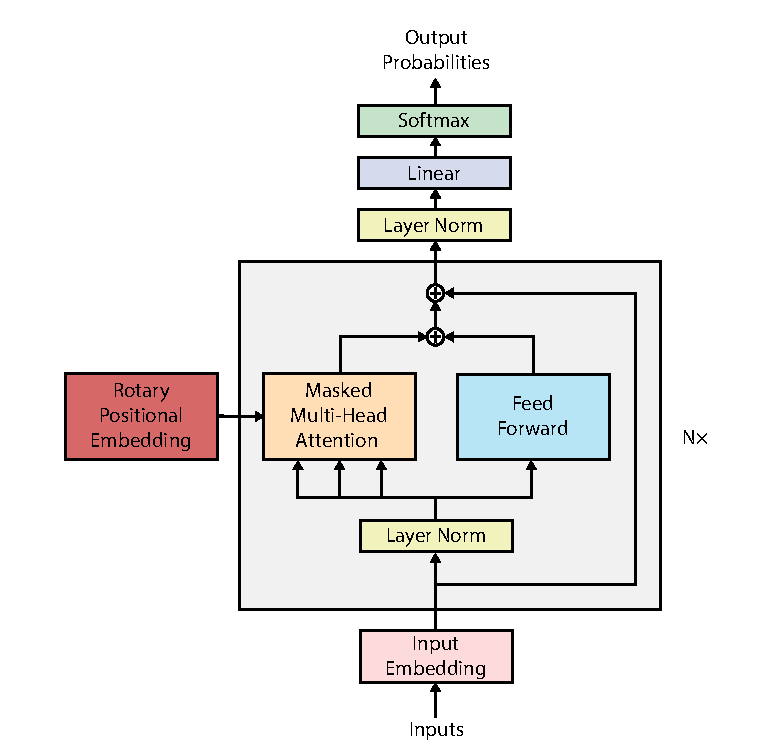
\includegraphics[width=0.8\textwidth]{figures/gpt-j_architecture.pdf}
    \caption{Diagram of GPT-J model architecture.}
    \label{fig:gpt-j-architecture}
\end{figure}

\subsubsection{Requirements}
\label{sec:requirements}
To load the GPT-J model in float32 precision, one would need at least 2x the model size of CPU RAM: 1x for the initial weights and another 1x to load the checkpoint. So for just loading the GPT-J model, it would require at least 48GB of CPU RAM. To reduce the memory footprint, one can load the model in half-precision.

GPU needs around 40GB of GPU memory to load the model. For training/fine-tuning the model, it would require significantly more GPU RAM. For example, the Adam optimizer makes four copies of the model: model, gradients, average and the squared average of gradients. Hence, it would take 4x model size GPU memory, even with mixed precision as gradient updates are in fp32. Further, this doesn't include the activations and data batches which would require some more GPU RAM. Hence, solutions like DeepSpeed \cite{deepspeed} needs to be used for training/fine-tuning such large models.

If a GPU with mixed precision capabilities (architecture Pascal or more recent) is available, one can use mixed precision training with PyTorch 1.6.0 or later, or by installing the Apex library for previous versions. If using an NVIDIA “Ampere” GPU architecture, the \acrfull{bf16} floating-point format can be used. Using mixed precision training usually results in 2x-speedup for training with the same final results.

\subsubsection{Pre-training}
Pre-training is defined as "Training in advance". By first training the model on a huge dataset, the model can then be fine-tuned on a much smaller dataset. This is so-called transfer learning. The pre-training procedure used for GPT class models is called \acrfull{clm} \cite{radford2018improving}. The model reads the text input in order and then tries to predict the next word. The model is fed a complete text element (input sequence) all at once, and then internal masking is applied to prevent the model from cheating by looking at future tokens. For more details on the inner workings of the training procedure, see \cref{sec:transformer-training}.

\subsection{Fine-tuning design}
\label{sec:rq1-fine-tuning-design}
To refine the pre-trained GPT-J-6B model for generating \acrshort{sc} code, the model needs to be fine-tuned on \acrshortpl{sc}. This should allow the model to adapt its existing knowledge gained from the pre-training procedure to produce high-quality \acrshort{sc} code. The fine-tuning procedure used is similar to that of the pre-training procedure. However, instead of using the Pile, a custom dataset of \acrshortpl{sc} needs to be constructed for use. The dataset then needs to be shuffled, before \acrshortpl{sc} are fed to the model for training. To ensure the validity of the model's performance, the dataset used needs to be split into separate sets for training, validation and testing. In this thesis, 80\% of the data will be used for testing, 10\% for validation, and 10\% for testing. After the model is fine-tuned, it should be able to auto-regressively generate \acrshortpl{sc} code. Due to the share size of the selected model (see \cref{sec:requirements}), no hyper-parameter optimization was performed. All hyper-parameters were set to their default values, as used for pre-training.

\section{Design for RQ2}
\label{sec:design-for-rq2}
This section describes the design for research question 2. The proposed method for generating secure \acrshort{sc} code with transformer models is described in \cref{sec:security-conditioning}. Then, the design of the fine-tuning process is described in \cref{sec:rq1-fine-tuning-design}.

\subsection{Security Conditioning}
\label{sec:security-conditioning}
When training a large language model on several gigabytes of open-source code, it is safe to assume that large portions of this code are not safe and contains vulnerabilities. For example, \textcite{durieux2020empirical} analyzed 47.587 real \acrshortpl{sc} with 9 automatic analysis tools. From these, 97\% of the contracts are tagged as vulnerable. This can result in a biased model that may produce a lot of vulnerable code. The idea of this thesis is to use a technique, named security conditioning, to reduce and mitigate this problem. 

The security conditioning is done by prepending a special security label to each of the records in the training data. This way, the model can learn to associate these tokens with either secure or vulnerable code. This way, by also using the labels when generating code, the model may be able to condition whether to produce safe or vulnerable code.

\subsection{Fine-tuning design}
\label{sec:rq2-fine-tuning-design}
For fine-tuning the pre-trained model with security conditioning, much of the same procedure as in \cref{sec:rq1-fine-tuning-design} is used. This makes it possible to validate the technique, by comparing the secured model with the "unsecured" model developed in RQ1. The primary difference is that the dataset records need to be labeled as secure or vulnerable. Before training, the dataset is shuffled and the \acrshortpl{sc} are fed to the model for training. To ensure the validity of the model's performance, the dataset needs to be split into separate sets for training, validation and testing. In this thesis, 80\% of the data will be used for testing, 10\% for validation, and 10\% for testing. To be able to The same hyperparameters used for as in \cref{sec:rq1-fine-tuning-design} no hyper-parameter optimization was performed. All hyper-parameters were set to their default values, as used for pre-training.

After the model is fine-tuned, it should be able to auto-regressively generate \acrshortpl{sc} code. To invoke the security conditioning, one only needs to prepend the security label to the input text.

\section{Technology}
\label{sec:technology}
Following is an overview of the different technologies applied in this project, both software and hardware.

\subsection{Software}
\label{sec:software}
During the selection of the language modeling library for use in this project, several considerations were made. Firstly, due to the huge size of the model, the library needed to support distributed GPU training. It had to be flexible and scalable, without sacrificing too much on speed. The transformers \cite{transformers} library by Hugging Face \cite{huggingface} fulfilled these conditions. The library provides flexible and easy-to-use solutions. It also supports integration with DeepSpeed \cite{deepspeed}, a deep learning optimization library by Microsoft \cite{microsoft} that makes distributed training and inference easy, efficient, and effective. The Hugging Face ecosystem also provides the Datasets and Tokenizers libraries, streamlining and significantly simplifying the use of large datasets.

\paragraph{DeepSpeed}
\label{par:deepspeed}
The deep learning optimization library DeepSpeed \cite{deepspeed} is used for training. It facilitates both distributed training, mixed precision and gradient accumulation, providing significant speedup of the training process while still being able to fit the model into the GPU memory available. The main workhorse of DeepSpeed is the \acrfull{zero} \cite{zero}. \acrshort{zero} comes with three incremental optimization stages: stage 1 (\acrshort{zero}-1), stage 2(\acrshort{zero}-2) and stage 3(\acrshort{zero}-3).

\begin{itemize}
    \item \textbf{Stage 1}: partitions the optimizer states across the processes, so each process only updates its partition.
    \item \textbf{Stage 2}: partitions the reduced gradients for updating the model weights, so that each process only retains the gradients corresponding to its own portion of the optimizer states.
    \item \textbf{Stage 3}: partitions the model parameters across the processes. They are automatically collected and partitioned during forward and backward passes.
\end{itemize}

\noindent
For training exceptionally large models, DeepSpeed also provides heterogeneous memory technologies based on \acrshort{zero}. This includes \acrshort{zero}-Offload for \acrshort{zero}-2 and \acrshort{zero}-Infinity \cite{zeroinfinity} for \acrshort{zero}-3. \acrshort{zero}-Offload offloads the optimizer memory and computation from the GPU to the host CPU. \acrshort{zero}-Infinity is an upgraded version of \acrshort{zero}-Offload that also allows for offloading to \gls{nvme} memory. DeepSpeed \acrshort{zero} makes it possible to train trillion parameter models \cite{zeroinfinity}. However, each optimization stage comes with a performance cost, slowing down the training process. DeepSpeed also provides support for mixed-precision training \cite{mixedprecision}. Mixed-precision training is the use of lower-precision operations (\acrshort{fp16} and \acrshort{bf16}) in a model during training. This both makes it run faster and uses less memory.

\subsection{Hardware resources}
\label{sec:hardware-resources}

The High Performance Computing Platform IDUN \cite{epic} is used for a lot of the tasks in this thesis, especially for the training of the model. IDUN full-fills the requirements defined in \cref{sec:requirements}.

\begin{figure}[htp]
    \centering
    \includegraphics[width=\textwidth]{figures/idun.jpeg}
    \caption{Image of IDUN \cite{idun2}}
    \label{fig:idun}
\end{figure}

%\chapter{Research implementation}
\label{chap:implementation}

\section{Data}
\label{sec:data}
This chapter introduces the necessary background information for this study. First, a brief introduction to blockchain technology is provided in \cref{sec:blockchain} and then the concept of \acrfullpl{sc} is introduced in \cref{sec:smart-contract}. Finally, in \cref{sec:smart-contract-vulnerabilities}, the most popular \acrshort{sc} vulnerabilities are described.

\subsection{Smart contract downloader}
\label{sec:smart-contract-downloader}
\url{https://github.com/andstor/smart-contract-downloader}


The largest provider of verified \acrshortpl{sc} is Etherscan. This website provides a list of all verified \acrshortpl{sc} on the blockchain. More on their service...... Etherscan provides a API for downloading verified Smart Contracts. The API is available at \url{https://api.etherscan.io/api}.

In order to download the \acrshortpl{sc} from Etherscan, a tool we need to provide the \acrshortpl{sc} address. The address is the first part of the \acrshortpl{sc} code. The address is the first part of the \acrshortpl{sc} code.

The following code snippet is a Google BigQuery query. It will select all \acrshortpl{sc} addresses on the Ethereum blockchain that has at least one transaction. This query was run on the 1st of April 2022, and the result was downloaded as a CSV file, and is available at \url{https://huggingface.co/datasets/andstor/smart_contracts/blob/main/contract_addresses.csv}. The CSV file is then used to download the \acrshortpl{sc} from Etherscan.

\begin{lstlisting}[
    caption={Google BigQuery query for selecting all \acrlong{sc} addresses on Ethereum that has at least one transaction.},
    label=lst:reentrancy,
    language=SQL]
SELECT contracts.address, COUNT(1) AS tx_count
FROM `bigquery-public-data.crypto_ethereum.contracts` AS contracts
JOIN `bigquery-public-data.crypto_ethereum.transactions` AS transactions 
      ON (transactions.to_address = contracts.address)
GROUP BY contracts.address
ORDER BY tx_count DESC
}
\end{lstlisting}

\todo{Include img of the processing script output}
Saved to file for simple reestarrting, multiprocessing and parallelization.

The total number of files generated by the downloading program was 5,810,042. In order to efficiently process these, all files were combined into a tarfile. A processing script was then created for filtering out all "empty" files. These correspond to a contract address on Ethereum that has not been verified on Etherscan.io. A total of 3,592,350 files were empty, making the source code of 38,17\% of the deployed contracts on Ethereum available. Each non-empty file is then parsed and the contract data is extracted. This extraction process is rather complicated, as smart contract sources come in a wide variety of flavors and formats.

\subsubsection{Normalization}
The most common is a contract written the Solidity language with  a single contract "entry"  \todo{Find a better name for contract keyword}. However, a single contrract file can contain multtiple contracts, making use of properties like inheritance etc.. The source code contracts can also be split over multiple files, a formmat rreefered to as "Multi file". When compiling thtese, the source code files aree "flattened" into a single contract file before compiliattion. Anotther flavour is hte JSON format, which is a language that is used to describe the \acrshortpl{sc}. Here the sourcecode is structured in tthe in the JSON code. Smart contracts can also be vritten in the Vyper language. Vyper is .... \todo{explain vyper}.


\begin{lstlisting}[
    caption={Solidity standard JSON Input format.},
    label=lst:flattened-dataset-cmd,
    language=JSON]
{
    "sources": {/* ... */},
    "settings": {
        "optimizer": {/* ... */},
        "evmVersion": "<VERSION>"
    }
}
\end{lstlisting}

All of the above formats are processed by the processing script, normalizing the contract source code to a single "flattened" contract file. The source code, along with the contract metadata, is then saved across multiple Parquet files, each consisting of 30000 "flattened" contracts. A total of 2,217,692 smart contracts were successfully parsed and normalized.

\subsubsection{Duplication filtering}
\label{sec:duplication-filtering}
A large quantity of Smart Contracts contains duplicated code. Primarily, this is due to the frequent use of library code, such as Safemath and ... \todo{Reference libraries}. Etherscan requires the library code used in a contract to be embedded in the source code. Filtering is applied to produce a dataset with a mostly unique contract source code to mitigate this. This filtering is done by calculating the string distance between the source code. Due to the rather large amount of contracts (\~2 million), the comparison is only made within groups of contracts. These groups are defined by grouping on the "contract\_name" for the \textit{flattened} dataset, and by "file\_name" for the \textit{inflated} dataset. These datasets will be discssed in detail in the following sections.

The actual code filtering is done by applying a token-based similarity algorithm named Jacard Index. The algorithm is computationally efficient and can be used to filter out \acrshortpl{sc} that are not similar to the query. The Jacard Index is a measure of the similarity between two sets. The Jacard Index is defined as the ratio of the size of the intersection to the size of the union of the two sets.


\subsection{Datasets}
\label{sec:datasets}
This section describes the datasets used and created in this study.

\subsubsection{The Pile}
\label{sec:the-pile}
Describe the  PILE...  It consists of among others, a lot of data from GitHub. HHowever, only x\% of the data is smart contracts (Solidity). Hence there is a need for a dataset made up of smart contracts. --> existing datasets....

\begin{figure}[htp]
    \centering
    \includegraphics[width=\textwidth]{figures/Treemap-of-Pile-components-by-effective-size.png}
    \caption{Treemap of Pile components by effective size. SOURCE FROM THEPILE paper}
    \label{fig:flowchart}
\end{figure}


\subsubsection{Verified Smart Contracts}
\label{sec:verified-smart-contracts}
\url{https://github.com/andstor/verified-smart-contracts}
\url{https://huggingface.co/datasets/andstor/smart_contracts}

The Verified Smart Contracts dataset is a dataset consisting of verified Smart Contracts from Etherscan.io. This is real smmart contracts that are deployed to the Ethereum blockchain. A set of 100,000 to 200,000 contracts are provided, containing both Solidity and Vyper code.

\cref{tab:verified-smart-contracts-metrics} shows the metrics of the various (sub)datasets.

\begin{table}
    %\newcolumntype{Y}{>{\centering\arraybackslash}X}
    \def\arraystretch{1.5}
    \small
    \centering
    \caption{Verified Smart Contracts Metrics}
    \label{tab:verified-smart-contracts-metrics}
    \begin{tabularx}{\textwidth}{XXXX}
        \toprule
        \textbf{Component} & \textbf{Size} &  \textbf{Num rows} & \textbf{LoC*}\\
        \midrule
        Raw & 0.80 GiB & 2,217,692 & 839,665,295\\
        Flattened & 1.16 GiB & 136,969 & 97,529,473\\
        Inflated & 0.76 GiB & 186,397 & 53,843,305\\
        Parsed & 4.44 GiB & 4,434,014 & 29,965,185\\
        \bottomrule
    \end{tabularx}
\end{table}

LoC refers to the lines of source\_code. The Parsed dataset counts lines of func\_code + func\_documentation.

\paragraph{Raw}
\label{sec:verified-smart-contracts-raw}
The raw dataset contains mostly the raw data from Etherscan, downloaded with the smart-contract-downlader tool, as described in \cref{sec:smart-contract-downloader}. All different contract formats (JSON, multi-file, etc.) are normalized to a flattened source code structure. 

\todo{Add stats on the raw dataset}

\paragraph{Flattened}
\label{sec:verified-smart-contracts-flattened}

The flattened dataset is a filtered version  of the Raw dataset\cref{sec:verified-smart-contracts-raw}. It contains smart contracts, where every contract contains all required library code. Each "file" is marked in the source code with a comment stating the original file path: //File: path/to/file.sol. These are then filtered for uniqueness with a similarity threshold of 0.9. This means that all contracts whose code shares more than 90\% of the tokens will be discarded. The low uniqueness requirement is due to the often large amount of embedded library code. If the requirement is set to high, the actual contract code will be negligible compared to the library code. Most contracts will be discarded, and the resulting dataset would contain mostly unique library code. However, the dataset as a whole will have a large amount of duplicated libray code. From the 2,217,692 contracts, 2,080,723 duplications are found, giving a duplication percentage of 93.82\%. The resulting dataset consists of 136,969 contracts.

%Processing: 100%|██████| 74/74 [20:22<00:00, 16.51s/it, dupes=2081081/2217692 (93.84%)]

The following command prooduces the flattened dataset:

\lstinline[language=Python]!python script/filter_data.py -s parquet -o data/flattened --threshold 0.9!


\begin{lstlisting}[
    caption={Solidity standard JSON Input format.},
    label=lst:flattened-dataset-cmd,
    language=JSON]
{
  'contract_name': 'MiaKhalifaDAO',
  'contract_address': '0xb3862ca215d5ed2de22734ed001d701adf0a30b4',
  'language': 'Solidity',
  'source_code': '// File: @openzeppelin/contracts/utils/Strings.sol\r\n\r\n\r\n// OpenZeppelin Contracts v4.4.1 (utils/Strings.sol)\r\n\r\npragma solidity ^0.8.0;\r\n\r\n/**\r\n * @dev String operations.\r\n */\r\nlibrary Strings {\r\n...',
  'abi': '[{"inputs":[{"internalType":"uint256","name":"maxBatchSize_","type":"uint256"}...]',
  'compiler_version': 'v0.8.7+commit.e28d00a7',
  'optimization_used': False,
  'runs': 200,
  'constructor_arguments': '000000000000000000000000000000000000000000000000000000000000000a000...',
  'evm_version': 'Default',
  'library': '',
  'license_type': 'MIT',
  'proxy': False,
  'implementation': '',
  'swarm_source': 'ipfs://e490df69bd9ca50e1831a1ac82177e826fee459b0b085a00bd7a727c80d74089'
}
\end{lstlisting}

\begin{figure}[htbp]
    \centering
    %% Creator: Matplotlib, PGF backend
%%
%% To include the figure in your LaTeX document, write
%%   \input{<filename>.pgf}
%%
%% Make sure the required packages are loaded in your preamble
%%   \usepackage{pgf}
%%
%% and, on pdftex
%%   \usepackage[utf8]{inputenc}\DeclareUnicodeCharacter{2212}{-}
%%
%% or, on luatex and xetex
%%   \usepackage{unicode-math}
%%
%% Figures using additional raster images can only be included by \input if
%% they are in the same directory as the main LaTeX file. For loading figures
%% from other directories you can use the `import` package
%%   \usepackage{import}
%%
%% and then include the figures with
%%   \import{<path to file>}{<filename>.pgf}
%%
%% Matplotlib used the following preamble
%%
\begingroup%
\makeatletter%
\begin{pgfpicture}%
\pgfpathrectangle{\pgfpointorigin}{\pgfqpoint{3.378613in}{3.378613in}}%
\pgfusepath{use as bounding box, clip}%
\begin{pgfscope}%
\pgfsetbuttcap%
\pgfsetmiterjoin%
\definecolor{currentfill}{rgb}{1.000000,1.000000,1.000000}%
\pgfsetfillcolor{currentfill}%
\pgfsetlinewidth{0.000000pt}%
\definecolor{currentstroke}{rgb}{1.000000,1.000000,1.000000}%
\pgfsetstrokecolor{currentstroke}%
\pgfsetdash{}{0pt}%
\pgfpathmoveto{\pgfqpoint{0.000000in}{0.000000in}}%
\pgfpathlineto{\pgfqpoint{3.378613in}{0.000000in}}%
\pgfpathlineto{\pgfqpoint{3.378613in}{3.378613in}}%
\pgfpathlineto{\pgfqpoint{0.000000in}{3.378613in}}%
\pgfpathclose%
\pgfusepath{fill}%
\end{pgfscope}%
\begin{pgfscope}%
\pgfsetbuttcap%
\pgfsetmiterjoin%
\definecolor{currentfill}{rgb}{0.925882,1.000000,0.634902}%
\pgfsetfillcolor{currentfill}%
\pgfsetfillopacity{0.700000}%
\pgfsetlinewidth{0.000000pt}%
\definecolor{currentstroke}{rgb}{0.000000,0.000000,0.000000}%
\pgfsetstrokecolor{currentstroke}%
\pgfsetstrokeopacity{0.700000}%
\pgfsetdash{}{0pt}%
\pgfpathmoveto{\pgfqpoint{2.751880in}{1.697753in}}%
\pgfpathcurveto{\pgfqpoint{2.751880in}{1.710594in}}{\pgfqpoint{2.751638in}{1.723433in}}{\pgfqpoint{2.751153in}{1.736265in}}%
\pgfpathcurveto{\pgfqpoint{2.750668in}{1.749097in}}{\pgfqpoint{2.749941in}{1.761918in}}{\pgfqpoint{2.748973in}{1.774723in}}%
\pgfpathlineto{\pgfqpoint{2.240256in}{1.736238in}}%
\pgfpathcurveto{\pgfqpoint{2.240740in}{1.729836in}}{\pgfqpoint{2.241104in}{1.723425in}}{\pgfqpoint{2.241346in}{1.717009in}}%
\pgfpathcurveto{\pgfqpoint{2.241588in}{1.710593in}}{\pgfqpoint{2.241709in}{1.704173in}}{\pgfqpoint{2.241709in}{1.697753in}}%
\pgfpathlineto{\pgfqpoint{2.751880in}{1.697753in}}%
\pgfpathclose%
\pgfusepath{fill}%
\end{pgfscope}%
\begin{pgfscope}%
\pgfsetbuttcap%
\pgfsetmiterjoin%
\definecolor{currentfill}{rgb}{0.882745,0.000000,0.111414}%
\pgfsetfillcolor{currentfill}%
\pgfsetfillopacity{0.700000}%
\pgfsetlinewidth{0.000000pt}%
\definecolor{currentstroke}{rgb}{0.000000,0.000000,0.000000}%
\pgfsetstrokecolor{currentstroke}%
\pgfsetstrokeopacity{0.700000}%
\pgfsetdash{}{0pt}%
\pgfpathmoveto{\pgfqpoint{2.748973in}{1.774723in}}%
\pgfpathcurveto{\pgfqpoint{2.735160in}{1.957309in}}{\pgfqpoint{2.672448in}{2.132855in}}{\pgfqpoint{2.567445in}{2.282865in}}%
\pgfpathcurveto{\pgfqpoint{2.462442in}{2.432875in}}{\pgfqpoint{2.318970in}{2.551890in}}{\pgfqpoint{2.152142in}{2.627370in}}%
\pgfpathcurveto{\pgfqpoint{1.985315in}{2.702851in}}{\pgfqpoint{1.801205in}{2.732050in}}{\pgfqpoint{1.619210in}{2.711892in}}%
\pgfpathcurveto{\pgfqpoint{1.437215in}{2.691734in}}{\pgfqpoint{1.263958in}{2.622951in}}{\pgfqpoint{1.117692in}{2.512792in}}%
\pgfpathcurveto{\pgfqpoint{0.971427in}{2.402632in}}{\pgfqpoint{0.857477in}{2.255104in}}{\pgfqpoint{0.787848in}{2.085752in}}%
\pgfpathcurveto{\pgfqpoint{0.718218in}{1.916399in}}{\pgfqpoint{0.695444in}{1.731384in}}{\pgfqpoint{0.721923in}{1.550201in}}%
\pgfpathcurveto{\pgfqpoint{0.748403in}{1.369017in}}{\pgfqpoint{0.823172in}{1.198259in}}{\pgfqpoint{0.938355in}{1.055916in}}%
\pgfpathcurveto{\pgfqpoint{1.053538in}{0.913572in}}{\pgfqpoint{1.204942in}{0.804825in}}{\pgfqpoint{1.376615in}{0.741131in}}%
\pgfpathlineto{\pgfqpoint{1.554077in}{1.219442in}}%
\pgfpathcurveto{\pgfqpoint{1.468240in}{1.251289in}}{\pgfqpoint{1.392538in}{1.305663in}}{\pgfqpoint{1.334947in}{1.376834in}}%
\pgfpathcurveto{\pgfqpoint{1.277356in}{1.448006in}}{\pgfqpoint{1.239971in}{1.533385in}}{\pgfqpoint{1.226731in}{1.623977in}}%
\pgfpathcurveto{\pgfqpoint{1.213491in}{1.714569in}}{\pgfqpoint{1.224879in}{1.807076in}}{\pgfqpoint{1.259693in}{1.891752in}}%
\pgfpathcurveto{\pgfqpoint{1.294508in}{1.976429in}}{\pgfqpoint{1.351483in}{2.050192in}}{\pgfqpoint{1.424616in}{2.105272in}}%
\pgfpathcurveto{\pgfqpoint{1.497748in}{2.160352in}}{\pgfqpoint{1.584377in}{2.194743in}}{\pgfqpoint{1.675374in}{2.204822in}}%
\pgfpathcurveto{\pgfqpoint{1.766372in}{2.214902in}}{\pgfqpoint{1.858427in}{2.200302in}}{\pgfqpoint{1.941841in}{2.162562in}}%
\pgfpathcurveto{\pgfqpoint{2.025254in}{2.124821in}}{\pgfqpoint{2.096991in}{2.065314in}}{\pgfqpoint{2.149492in}{1.990309in}}%
\pgfpathcurveto{\pgfqpoint{2.201994in}{1.915304in}}{\pgfqpoint{2.233349in}{1.827531in}}{\pgfqpoint{2.240256in}{1.736238in}}%
\pgfpathlineto{\pgfqpoint{2.748973in}{1.774723in}}%
\pgfpathclose%
\pgfusepath{fill}%
\end{pgfscope}%
\begin{pgfscope}%
\pgfsetbuttcap%
\pgfsetmiterjoin%
\definecolor{currentfill}{rgb}{0.000000,0.786667,0.312353}%
\pgfsetfillcolor{currentfill}%
\pgfsetfillopacity{0.700000}%
\pgfsetlinewidth{0.000000pt}%
\definecolor{currentstroke}{rgb}{0.000000,0.000000,0.000000}%
\pgfsetstrokecolor{currentstroke}%
\pgfsetstrokeopacity{0.700000}%
\pgfsetdash{}{0pt}%
\pgfpathmoveto{\pgfqpoint{1.376615in}{0.741131in}}%
\pgfpathcurveto{\pgfqpoint{1.391448in}{0.735628in}}{\pgfqpoint{1.406407in}{0.730470in}}{\pgfqpoint{1.421480in}{0.725663in}}%
\pgfpathcurveto{\pgfqpoint{1.436553in}{0.720855in}}{\pgfqpoint{1.451736in}{0.716398in}}{\pgfqpoint{1.467016in}{0.712297in}}%
\pgfpathlineto{\pgfqpoint{1.599278in}{1.205025in}}%
\pgfpathcurveto{\pgfqpoint{1.591638in}{1.207076in}}{\pgfqpoint{1.584046in}{1.209304in}}{\pgfqpoint{1.576510in}{1.211708in}}%
\pgfpathcurveto{\pgfqpoint{1.568973in}{1.214112in}}{\pgfqpoint{1.561494in}{1.216690in}}{\pgfqpoint{1.554077in}{1.219442in}}%
\pgfpathlineto{\pgfqpoint{1.376615in}{0.741131in}}%
\pgfpathclose%
\pgfusepath{fill}%
\end{pgfscope}%
\begin{pgfscope}%
\pgfsetbuttcap%
\pgfsetmiterjoin%
\definecolor{currentfill}{rgb}{0.930307,0.285685,0.029301}%
\pgfsetfillcolor{currentfill}%
\pgfsetfillopacity{0.700000}%
\pgfsetlinewidth{0.000000pt}%
\definecolor{currentstroke}{rgb}{0.000000,0.000000,0.000000}%
\pgfsetstrokecolor{currentstroke}%
\pgfsetstrokeopacity{0.700000}%
\pgfsetdash{}{0pt}%
\pgfpathmoveto{\pgfqpoint{1.467016in}{0.712297in}}%
\pgfpathcurveto{\pgfqpoint{1.642990in}{0.665061in}}{\pgfqpoint{1.828446in}{0.665812in}}{\pgfqpoint{2.004032in}{0.714471in}}%
\pgfpathcurveto{\pgfqpoint{2.179617in}{0.763130in}}{\pgfqpoint{2.339006in}{0.857944in}}{\pgfqpoint{2.465565in}{0.989020in}}%
\pgfpathlineto{\pgfqpoint{2.098552in}{1.343386in}}%
\pgfpathcurveto{\pgfqpoint{2.035272in}{1.277849in}}{\pgfqpoint{1.955578in}{1.230441in}}{\pgfqpoint{1.867785in}{1.206112in}}%
\pgfpathcurveto{\pgfqpoint{1.779992in}{1.181782in}}{\pgfqpoint{1.687265in}{1.181407in}}{\pgfqpoint{1.599278in}{1.205025in}}%
\pgfpathlineto{\pgfqpoint{1.467016in}{0.712297in}}%
\pgfpathclose%
\pgfusepath{fill}%
\end{pgfscope}%
\begin{pgfscope}%
\pgfsetbuttcap%
\pgfsetmiterjoin%
\definecolor{currentfill}{rgb}{0.063700,0.382199,0.851986}%
\pgfsetfillcolor{currentfill}%
\pgfsetfillopacity{0.700000}%
\pgfsetlinewidth{0.000000pt}%
\definecolor{currentstroke}{rgb}{0.000000,0.000000,0.000000}%
\pgfsetstrokecolor{currentstroke}%
\pgfsetstrokeopacity{0.700000}%
\pgfsetdash{}{0pt}%
\pgfpathmoveto{\pgfqpoint{2.465565in}{0.989020in}}%
\pgfpathcurveto{\pgfqpoint{2.556545in}{1.083247in}}{\pgfqpoint{2.628535in}{1.194117in}}{\pgfqpoint{2.677597in}{1.315562in}}%
\pgfpathcurveto{\pgfqpoint{2.726659in}{1.437008in}}{\pgfqpoint{2.751880in}{1.566772in}}{\pgfqpoint{2.751880in}{1.697753in}}%
\pgfpathlineto{\pgfqpoint{2.241709in}{1.697753in}}%
\pgfpathcurveto{\pgfqpoint{2.241709in}{1.632262in}}{\pgfqpoint{2.229099in}{1.567380in}}{\pgfqpoint{2.204568in}{1.506658in}}%
\pgfpathcurveto{\pgfqpoint{2.180037in}{1.445935in}}{\pgfqpoint{2.144042in}{1.390500in}}{\pgfqpoint{2.098552in}{1.343386in}}%
\pgfpathlineto{\pgfqpoint{2.465565in}{0.989020in}}%
\pgfpathclose%
\pgfusepath{fill}%
\end{pgfscope}%
\begin{pgfscope}%
\pgfsetbuttcap%
\pgfsetmiterjoin%
\definecolor{currentfill}{rgb}{0.925882,1.000000,0.634902}%
\pgfsetfillcolor{currentfill}%
\pgfsetfillopacity{0.700000}%
\pgfsetlinewidth{0.000000pt}%
\definecolor{currentstroke}{rgb}{0.000000,0.000000,0.000000}%
\pgfsetstrokecolor{currentstroke}%
\pgfsetstrokeopacity{0.700000}%
\pgfsetdash{}{0pt}%
\pgfpathmoveto{\pgfqpoint{3.262050in}{1.697753in}}%
\pgfpathcurveto{\pgfqpoint{3.262050in}{1.717014in}}{\pgfqpoint{3.261687in}{1.736274in}}{\pgfqpoint{3.260960in}{1.755521in}}%
\pgfpathcurveto{\pgfqpoint{3.260233in}{1.774769in}}{\pgfqpoint{3.259143in}{1.794001in}}{\pgfqpoint{3.257690in}{1.813207in}}%
\pgfpathlineto{\pgfqpoint{2.748973in}{1.774723in}}%
\pgfpathcurveto{\pgfqpoint{2.749941in}{1.761918in}}{\pgfqpoint{2.750668in}{1.749097in}}{\pgfqpoint{2.751153in}{1.736265in}}%
\pgfpathcurveto{\pgfqpoint{2.751638in}{1.723433in}}{\pgfqpoint{2.751880in}{1.710594in}}{\pgfqpoint{2.751880in}{1.697753in}}%
\pgfpathlineto{\pgfqpoint{3.262050in}{1.697753in}}%
\pgfpathclose%
\pgfusepath{fill}%
\end{pgfscope}%
\begin{pgfscope}%
\pgfsetbuttcap%
\pgfsetmiterjoin%
\definecolor{currentfill}{rgb}{0.882745,0.000000,0.111414}%
\pgfsetfillcolor{currentfill}%
\pgfsetfillopacity{0.700000}%
\pgfsetlinewidth{0.000000pt}%
\definecolor{currentstroke}{rgb}{0.000000,0.000000,0.000000}%
\pgfsetstrokecolor{currentstroke}%
\pgfsetstrokeopacity{0.700000}%
\pgfsetdash{}{0pt}%
\pgfpathmoveto{\pgfqpoint{3.257690in}{1.813207in}}%
\pgfpathcurveto{\pgfqpoint{3.252513in}{1.881632in}}{\pgfqpoint{3.242741in}{1.949631in}}{\pgfqpoint{3.228439in}{2.016745in}}%
\pgfpathcurveto{\pgfqpoint{3.214137in}{2.083858in}}{\pgfqpoint{3.195338in}{2.149933in}}{\pgfqpoint{3.172168in}{2.214524in}}%
\pgfpathlineto{\pgfqpoint{2.691959in}{2.042267in}}%
\pgfpathcurveto{\pgfqpoint{2.707405in}{1.999207in}}{\pgfqpoint{2.719938in}{1.955156in}}{\pgfqpoint{2.729472in}{1.910414in}}%
\pgfpathcurveto{\pgfqpoint{2.739007in}{1.865672in}}{\pgfqpoint{2.745522in}{1.820339in}}{\pgfqpoint{2.748973in}{1.774723in}}%
\pgfpathlineto{\pgfqpoint{3.257690in}{1.813207in}}%
\pgfpathclose%
\pgfusepath{fill}%
\end{pgfscope}%
\begin{pgfscope}%
\pgfsetbuttcap%
\pgfsetmiterjoin%
\definecolor{currentfill}{rgb}{0.917292,0.307374,0.323876}%
\pgfsetfillcolor{currentfill}%
\pgfsetfillopacity{0.700000}%
\pgfsetlinewidth{0.000000pt}%
\definecolor{currentstroke}{rgb}{0.000000,0.000000,0.000000}%
\pgfsetstrokecolor{currentstroke}%
\pgfsetstrokeopacity{0.700000}%
\pgfsetdash{}{0pt}%
\pgfpathmoveto{\pgfqpoint{3.172168in}{2.214524in}}%
\pgfpathcurveto{\pgfqpoint{3.143867in}{2.293420in}}{\pgfqpoint{3.109133in}{2.369858in}}{\pgfqpoint{3.068316in}{2.443066in}}%
\pgfpathcurveto{\pgfqpoint{3.027499in}{2.516275in}}{\pgfqpoint{2.980737in}{2.586007in}}{\pgfqpoint{2.928502in}{2.651558in}}%
\pgfpathlineto{\pgfqpoint{2.529514in}{2.333623in}}%
\pgfpathcurveto{\pgfqpoint{2.564338in}{2.289922in}}{\pgfqpoint{2.595512in}{2.243434in}}{\pgfqpoint{2.622724in}{2.194628in}}%
\pgfpathcurveto{\pgfqpoint{2.649935in}{2.145823in}}{\pgfqpoint{2.673091in}{2.094864in}}{\pgfqpoint{2.691959in}{2.042267in}}%
\pgfpathlineto{\pgfqpoint{3.172168in}{2.214524in}}%
\pgfpathclose%
\pgfusepath{fill}%
\end{pgfscope}%
\begin{pgfscope}%
\pgfsetbuttcap%
\pgfsetmiterjoin%
\definecolor{currentfill}{rgb}{0.989063,0.592703,0.504860}%
\pgfsetfillcolor{currentfill}%
\pgfsetfillopacity{0.700000}%
\pgfsetlinewidth{0.000000pt}%
\definecolor{currentstroke}{rgb}{0.000000,0.000000,0.000000}%
\pgfsetstrokecolor{currentstroke}%
\pgfsetstrokeopacity{0.700000}%
\pgfsetdash{}{0pt}%
\pgfpathmoveto{\pgfqpoint{2.928502in}{2.651558in}}%
\pgfpathcurveto{\pgfqpoint{2.784634in}{2.832104in}}{\pgfqpoint{2.601763in}{2.977780in}}{\pgfqpoint{2.393626in}{3.077647in}}%
\pgfpathcurveto{\pgfqpoint{2.185488in}{3.177513in}}{\pgfqpoint{1.957427in}{3.229006in}}{\pgfqpoint{1.726572in}{3.228256in}}%
\pgfpathlineto{\pgfqpoint{1.728227in}{2.718088in}}%
\pgfpathcurveto{\pgfqpoint{1.882131in}{2.718588in}}{\pgfqpoint{2.034171in}{2.684260in}}{\pgfqpoint{2.172930in}{2.617682in}}%
\pgfpathcurveto{\pgfqpoint{2.311689in}{2.551104in}}{\pgfqpoint{2.433602in}{2.453987in}}{\pgfqpoint{2.529514in}{2.333623in}}%
\pgfpathlineto{\pgfqpoint{2.928502in}{2.651558in}}%
\pgfpathclose%
\pgfusepath{fill}%
\end{pgfscope}%
\begin{pgfscope}%
\pgfsetbuttcap%
\pgfsetmiterjoin%
\definecolor{currentfill}{rgb}{0.991894,0.815723,0.745126}%
\pgfsetfillcolor{currentfill}%
\pgfsetfillopacity{0.700000}%
\pgfsetlinewidth{0.000000pt}%
\definecolor{currentstroke}{rgb}{0.000000,0.000000,0.000000}%
\pgfsetstrokecolor{currentstroke}%
\pgfsetstrokeopacity{0.700000}%
\pgfsetdash{}{0pt}%
\pgfpathmoveto{\pgfqpoint{1.726572in}{3.228256in}}%
\pgfpathcurveto{\pgfqpoint{1.368074in}{3.227093in}}{\pgfqpoint{1.021135in}{3.100006in}}{\pgfqpoint{0.746712in}{2.869325in}}%
\pgfpathcurveto{\pgfqpoint{0.472288in}{2.638643in}}{\pgfqpoint{0.287451in}{2.318718in}}{\pgfqpoint{0.224675in}{1.965757in}}%
\pgfpathcurveto{\pgfqpoint{0.161899in}{1.612796in}}{\pgfqpoint{0.225089in}{1.248757in}}{\pgfqpoint{0.403144in}{0.937600in}}%
\pgfpathcurveto{\pgfqpoint{0.581199in}{0.626443in}}{\pgfqpoint{0.863041in}{0.387524in}}{\pgfqpoint{1.199153in}{0.262821in}}%
\pgfpathlineto{\pgfqpoint{1.376615in}{0.741131in}}%
\pgfpathcurveto{\pgfqpoint{1.152540in}{0.824267in}}{\pgfqpoint{0.964645in}{0.983546in}}{\pgfqpoint{0.845942in}{1.190984in}}%
\pgfpathcurveto{\pgfqpoint{0.727239in}{1.398422in}}{\pgfqpoint{0.685112in}{1.641115in}}{\pgfqpoint{0.726963in}{1.876422in}}%
\pgfpathcurveto{\pgfqpoint{0.768814in}{2.111729in}}{\pgfqpoint{0.892038in}{2.325013in}}{\pgfqpoint{1.074987in}{2.478801in}}%
\pgfpathcurveto{\pgfqpoint{1.257936in}{2.632588in}}{\pgfqpoint{1.489229in}{2.717313in}}{\pgfqpoint{1.728227in}{2.718088in}}%
\pgfpathlineto{\pgfqpoint{1.726572in}{3.228256in}}%
\pgfpathclose%
\pgfusepath{fill}%
\end{pgfscope}%
\begin{pgfscope}%
\pgfsetbuttcap%
\pgfsetmiterjoin%
\definecolor{currentfill}{rgb}{0.000000,0.786667,0.312353}%
\pgfsetfillcolor{currentfill}%
\pgfsetfillopacity{0.700000}%
\pgfsetlinewidth{0.000000pt}%
\definecolor{currentstroke}{rgb}{0.000000,0.000000,0.000000}%
\pgfsetstrokecolor{currentstroke}%
\pgfsetstrokeopacity{0.700000}%
\pgfsetdash{}{0pt}%
\pgfpathmoveto{\pgfqpoint{1.199153in}{0.262821in}}%
\pgfpathcurveto{\pgfqpoint{1.221403in}{0.254566in}}{\pgfqpoint{1.243841in}{0.246829in}}{\pgfqpoint{1.266451in}{0.239618in}}%
\pgfpathcurveto{\pgfqpoint{1.289060in}{0.232406in}}{\pgfqpoint{1.311835in}{0.225721in}}{\pgfqpoint{1.334755in}{0.219569in}}%
\pgfpathlineto{\pgfqpoint{1.467016in}{0.712297in}}%
\pgfpathcurveto{\pgfqpoint{1.451736in}{0.716398in}}{\pgfqpoint{1.436553in}{0.720855in}}{\pgfqpoint{1.421480in}{0.725663in}}%
\pgfpathcurveto{\pgfqpoint{1.406407in}{0.730470in}}{\pgfqpoint{1.391448in}{0.735628in}}{\pgfqpoint{1.376615in}{0.741131in}}%
\pgfpathlineto{\pgfqpoint{1.199153in}{0.262821in}}%
\pgfpathclose%
\pgfusepath{fill}%
\end{pgfscope}%
\begin{pgfscope}%
\pgfsetbuttcap%
\pgfsetmiterjoin%
\definecolor{currentfill}{rgb}{0.930307,0.285685,0.029301}%
\pgfsetfillcolor{currentfill}%
\pgfsetfillopacity{0.700000}%
\pgfsetlinewidth{0.000000pt}%
\definecolor{currentstroke}{rgb}{0.000000,0.000000,0.000000}%
\pgfsetstrokecolor{currentstroke}%
\pgfsetstrokeopacity{0.700000}%
\pgfsetdash{}{0pt}%
\pgfpathmoveto{\pgfqpoint{1.334755in}{0.219569in}}%
\pgfpathcurveto{\pgfqpoint{1.475152in}{0.181883in}}{\pgfqpoint{1.620204in}{0.164390in}}{\pgfqpoint{1.765535in}{0.167619in}}%
\pgfpathcurveto{\pgfqpoint{1.910866in}{0.170848in}}{\pgfqpoint{2.054998in}{0.194765in}}{\pgfqpoint{2.193582in}{0.238650in}}%
\pgfpathlineto{\pgfqpoint{2.039568in}{0.725018in}}%
\pgfpathcurveto{\pgfqpoint{1.947178in}{0.695761in}}{\pgfqpoint{1.851090in}{0.679816in}}{\pgfqpoint{1.754203in}{0.677664in}}%
\pgfpathcurveto{\pgfqpoint{1.657316in}{0.675511in}}{\pgfqpoint{1.560614in}{0.687173in}}{\pgfqpoint{1.467016in}{0.712297in}}%
\pgfpathlineto{\pgfqpoint{1.334755in}{0.219569in}}%
\pgfpathclose%
\pgfusepath{fill}%
\end{pgfscope}%
\begin{pgfscope}%
\pgfsetbuttcap%
\pgfsetmiterjoin%
\definecolor{currentfill}{rgb}{0.995815,0.464325,0.203521}%
\pgfsetfillcolor{currentfill}%
\pgfsetfillopacity{0.700000}%
\pgfsetlinewidth{0.000000pt}%
\definecolor{currentstroke}{rgb}{0.000000,0.000000,0.000000}%
\pgfsetstrokecolor{currentstroke}%
\pgfsetstrokeopacity{0.700000}%
\pgfsetdash{}{0pt}%
\pgfpathmoveto{\pgfqpoint{2.193582in}{0.238650in}}%
\pgfpathcurveto{\pgfqpoint{2.314418in}{0.276914in}}{\pgfqpoint{2.430034in}{0.330041in}}{\pgfqpoint{2.537772in}{0.396809in}}%
\pgfpathcurveto{\pgfqpoint{2.645509in}{0.463577in}}{\pgfqpoint{2.744537in}{0.543471in}}{\pgfqpoint{2.832577in}{0.634654in}}%
\pgfpathlineto{\pgfqpoint{2.465565in}{0.989020in}}%
\pgfpathcurveto{\pgfqpoint{2.406871in}{0.928232in}}{\pgfqpoint{2.340853in}{0.874969in}}{\pgfqpoint{2.269027in}{0.830457in}}%
\pgfpathcurveto{\pgfqpoint{2.197202in}{0.785945in}}{\pgfqpoint{2.120125in}{0.750527in}}{\pgfqpoint{2.039568in}{0.725018in}}%
\pgfpathlineto{\pgfqpoint{2.193582in}{0.238650in}}%
\pgfpathclose%
\pgfusepath{fill}%
\end{pgfscope}%
\begin{pgfscope}%
\pgfsetbuttcap%
\pgfsetmiterjoin%
\definecolor{currentfill}{rgb}{0.063700,0.382199,0.851986}%
\pgfsetfillcolor{currentfill}%
\pgfsetfillopacity{0.700000}%
\pgfsetlinewidth{0.000000pt}%
\definecolor{currentstroke}{rgb}{0.000000,0.000000,0.000000}%
\pgfsetstrokecolor{currentstroke}%
\pgfsetstrokeopacity{0.700000}%
\pgfsetdash{}{0pt}%
\pgfpathmoveto{\pgfqpoint{2.832577in}{0.634654in}}%
\pgfpathcurveto{\pgfqpoint{2.969047in}{0.775994in}}{\pgfqpoint{3.077034in}{0.942299in}}{\pgfqpoint{3.150626in}{1.124467in}}%
\pgfpathcurveto{\pgfqpoint{3.224219in}{1.306635in}}{\pgfqpoint{3.262050in}{1.501281in}}{\pgfqpoint{3.262050in}{1.697753in}}%
\pgfpathlineto{\pgfqpoint{2.751880in}{1.697753in}}%
\pgfpathcurveto{\pgfqpoint{2.751880in}{1.566772in}}{\pgfqpoint{2.726659in}{1.437008in}}{\pgfqpoint{2.677597in}{1.315562in}}%
\pgfpathcurveto{\pgfqpoint{2.628535in}{1.194117in}}{\pgfqpoint{2.556545in}{1.083247in}}{\pgfqpoint{2.465565in}{0.989020in}}%
\pgfpathlineto{\pgfqpoint{2.832577in}{0.634654in}}%
\pgfpathclose%
\pgfusepath{fill}%
\end{pgfscope}%
\begin{pgfscope}%
\definecolor{textcolor}{rgb}{0.000000,0.000000,0.000000}%
\pgfsetstrokecolor{textcolor}%
\pgfsetfillcolor{textcolor}%
\pgftext[x=2.445269in,y=1.724711in,left,]{\color{textcolor}\rmfamily\fontsize{9.000000}{10.800000}\selectfont E}%
\end{pgfscope}%
\begin{pgfscope}%
\definecolor{textcolor}{rgb}{0.000000,0.000000,0.000000}%
\pgfsetstrokecolor{textcolor}%
\pgfsetfillcolor{textcolor}%
\pgftext[x=1.301846in,y=2.268280in,right,]{\color{textcolor}\rmfamily\fontsize{9.000000}{10.800000}\selectfont H}%
\end{pgfscope}%
\begin{pgfscope}%
\definecolor{textcolor}{rgb}{0.000000,0.000000,0.000000}%
\pgfsetstrokecolor{textcolor}%
\pgfsetfillcolor{textcolor}%
\pgftext[x=1.514498in,y=1.017290in,right,]{\color{textcolor}\rmfamily\fontsize{9.000000}{10.800000}\selectfont L}%
\end{pgfscope}%
\begin{pgfscope}%
\definecolor{textcolor}{rgb}{0.000000,0.000000,0.000000}%
\pgfsetstrokecolor{textcolor}%
\pgfsetfillcolor{textcolor}%
\pgftext[x=1.922284in,y=1.009455in,left,]{\color{textcolor}\rmfamily\fontsize{9.000000}{10.800000}\selectfont M}%
\end{pgfscope}%
\begin{pgfscope}%
\definecolor{textcolor}{rgb}{0.000000,0.000000,0.000000}%
\pgfsetstrokecolor{textcolor}%
\pgfsetfillcolor{textcolor}%
\pgftext[x=2.393780in,y=1.430219in,left,]{\color{textcolor}\rmfamily\fontsize{9.000000}{10.800000}\selectfont S}%
\end{pgfscope}%
\begin{pgfscope}%
\definecolor{textcolor}{rgb}{0.000000,0.000000,0.000000}%
\pgfsetstrokecolor{textcolor}%
\pgfsetfillcolor{textcolor}%
\pgftext[x=2.938082in,y=1.743326in,left,]{\color{textcolor}\rmfamily\fontsize{9.000000}{10.800000}\selectfont E}%
\end{pgfscope}%
\begin{pgfscope}%
\definecolor{textcolor}{rgb}{0.000000,0.000000,0.000000}%
\pgfsetstrokecolor{textcolor}%
\pgfsetfillcolor{textcolor}%
\pgftext[x=2.912427in,y=1.949402in,left,]{\color{textcolor}\rmfamily\fontsize{9.000000}{10.800000}\selectfont H}%
\end{pgfscope}%
\begin{pgfscope}%
\definecolor{textcolor}{rgb}{0.000000,0.000000,0.000000}%
\pgfsetstrokecolor{textcolor}%
\pgfsetfillcolor{textcolor}%
\pgftext[x=2.786108in,y=2.285722in,left,]{\color{textcolor}\rmfamily\fontsize{9.000000}{10.800000}\selectfont HL}%
\end{pgfscope}%
\begin{pgfscope}%
\definecolor{textcolor}{rgb}{0.000000,0.000000,0.000000}%
\pgfsetstrokecolor{textcolor}%
\pgfsetfillcolor{textcolor}%
\pgftext[x=2.253852in,y=2.786336in,left,]{\color{textcolor}\rmfamily\fontsize{9.000000}{10.800000}\selectfont HM}%
\end{pgfscope}%
\begin{pgfscope}%
\definecolor{textcolor}{rgb}{0.000000,0.000000,0.000000}%
\pgfsetstrokecolor{textcolor}%
\pgfsetfillcolor{textcolor}%
\pgftext[x=0.542791in,y=1.909178in,right,]{\color{textcolor}\rmfamily\fontsize{9.000000}{10.800000}\selectfont HML}%
\end{pgfscope}%
\begin{pgfscope}%
\definecolor{textcolor}{rgb}{0.000000,0.000000,0.000000}%
\pgfsetstrokecolor{textcolor}%
\pgfsetfillcolor{textcolor}%
\pgftext[x=1.364636in,y=0.547446in,right,]{\color{textcolor}\rmfamily\fontsize{9.000000}{10.800000}\selectfont L}%
\end{pgfscope}%
\begin{pgfscope}%
\definecolor{textcolor}{rgb}{0.000000,0.000000,0.000000}%
\pgfsetstrokecolor{textcolor}%
\pgfsetfillcolor{textcolor}%
\pgftext[x=1.758358in,y=0.490647in,left,]{\color{textcolor}\rmfamily\fontsize{9.000000}{10.800000}\selectfont M}%
\end{pgfscope}%
\begin{pgfscope}%
\definecolor{textcolor}{rgb}{0.000000,0.000000,0.000000}%
\pgfsetstrokecolor{textcolor}%
\pgfsetfillcolor{textcolor}%
\pgftext[x=2.367567in,y=0.671453in,left,]{\color{textcolor}\rmfamily\fontsize{9.000000}{10.800000}\selectfont ML}%
\end{pgfscope}%
\begin{pgfscope}%
\definecolor{textcolor}{rgb}{0.000000,0.000000,0.000000}%
\pgfsetstrokecolor{textcolor}%
\pgfsetfillcolor{textcolor}%
\pgftext[x=2.851041in,y=1.245494in,left,]{\color{textcolor}\rmfamily\fontsize{9.000000}{10.800000}\selectfont S}%
\end{pgfscope}%
\end{pgfpicture}%
\makeatother%
\endgroup%

    \caption{Doughnut chart over the distribution of the vulnerability severities in the flattened dataset at different granularity levels, where each level occurs at least once in the \acrshort{sc}. The outer ring shows the additional security levels for each contract. For example, "HML" means that the contract has at least three vulnerabilities with the corresponding "High", "Medium", and "Low" security levels.}
\end{figure}


\begin{figure}[htbp]
    \centering
    \input{figures/flattened_vulnerabilities_bar.pgf}
    \caption{Distribution of vulnerabilities in the flattened dataset.}
\end{figure}

\paragraph{Inflated}
\label{sec:verified-smart-contracts-inflated}
The inflated dataset is also based on the raw dataset. Each contract file in the dataset is split into its original representative files. This mitigates a lot of the problems of the flattened dataset in terms of duplicated library code. The library code would, along with other imported contract files, be split into separate contract records. The 2,217,692 "raw" smart contracts are inflated to a total of 5,403,136 separate contract files. These are then grouped by "file\_name" and filtered for uniqueness with a similarity threshold of 0.9. This should produce a dataset with a large amount of unique source code, with low quantities of library code. A total of 5,216,739 duplications are found, giving a duplication percentage of 96.56\%. The resulting dataset consists of 186,397 contracts.

%Processing: 100%|██████| 74/74 [22:50<00:00, 18.52s/it, dupes=5217191/5403136 (96.56%)]


\lstinline[language=Python]!python script/filter_data.py -s parquet -o data/inflated --split-files --threshold 0.9!
dupes=5217191/5403136 (96.56%)


\begin{lstlisting}[
    caption={Solidity standard JSON Input format.},
    label=lst:flattened-dataset-cmd,
    language=JSON]
    {
        'contract_name': 'PinkLemonade',
        'file_path': 'PinkLemonade.sol',
        'contract_address': '0x9a5be3cc368f01a0566a613aad7183783cff7eec',
        'language': 'Solidity',
        'source_code': '/**\r\n\r\nt.me/pinklemonadecoin\r\n*/\r\n\r\n// SPDX-License-Identifier: MIT\r\npragma solidity ^0.8.0;\r\n\r\n\r\n/*\r\n * @dev Provides information about the current execution context, including the\r\n * sender of the transaction and its data. While these are generally available...',
        'abi': '[{"inputs":[],"stateMutability":"nonpayable","type":"constructor"}...]',
        'compiler_version': 'v0.8.4+commit.c7e474f2',
        'optimization_used': False,
        'runs': 200,
        'constructor_arguments': '',
        'evm_version': 'Default',
        'library': '',
        'license_type': 'MIT',
        'proxy': False,
        'implementation': '',
        'swarm_source': 'ipfs://eb0ac9491a04e7a196280fd27ce355a85d79b34c7b0a83ab606d27972a06050c'
      }
      
      
\end{lstlisting}

\begin{figure}[htbp]
    \centering
    %% Creator: Matplotlib, PGF backend
%%
%% To include the figure in your LaTeX document, write
%%   \input{<filename>.pgf}
%%
%% Make sure the required packages are loaded in your preamble
%%   \usepackage{pgf}
%%
%% and, on pdftex
%%   \usepackage[utf8]{inputenc}\DeclareUnicodeCharacter{2212}{-}
%%
%% or, on luatex and xetex
%%   \usepackage{unicode-math}
%%
%% Figures using additional raster images can only be included by \input if
%% they are in the same directory as the main LaTeX file. For loading figures
%% from other directories you can use the `import` package
%%   \usepackage{import}
%%
%% and then include the figures with
%%   \import{<path to file>}{<filename>.pgf}
%%
%% Matplotlib used the following preamble
%%
\begingroup%
\makeatletter%
\begin{pgfpicture}%
\pgfpathrectangle{\pgfpointorigin}{\pgfqpoint{3.465474in}{3.767802in}}%
\pgfusepath{use as bounding box, clip}%
\begin{pgfscope}%
\pgfsetbuttcap%
\pgfsetmiterjoin%
\definecolor{currentfill}{rgb}{1.000000,1.000000,1.000000}%
\pgfsetfillcolor{currentfill}%
\pgfsetlinewidth{0.000000pt}%
\definecolor{currentstroke}{rgb}{1.000000,1.000000,1.000000}%
\pgfsetstrokecolor{currentstroke}%
\pgfsetdash{}{0pt}%
\pgfpathmoveto{\pgfqpoint{0.000000in}{-0.000000in}}%
\pgfpathlineto{\pgfqpoint{3.465474in}{-0.000000in}}%
\pgfpathlineto{\pgfqpoint{3.465474in}{3.767802in}}%
\pgfpathlineto{\pgfqpoint{0.000000in}{3.767802in}}%
\pgfpathclose%
\pgfusepath{fill}%
\end{pgfscope}%
\begin{pgfscope}%
\pgfsetbuttcap%
\pgfsetmiterjoin%
\definecolor{currentfill}{rgb}{0.882745,0.000000,0.111414}%
\pgfsetfillcolor{currentfill}%
\pgfsetfillopacity{0.700000}%
\pgfsetlinewidth{0.000000pt}%
\definecolor{currentstroke}{rgb}{0.000000,0.000000,0.000000}%
\pgfsetstrokecolor{currentstroke}%
\pgfsetstrokeopacity{0.700000}%
\pgfsetdash{}{0pt}%
\pgfpathmoveto{\pgfqpoint{2.667253in}{2.128968in}}%
\pgfpathcurveto{\pgfqpoint{2.667253in}{2.388922in}}{\pgfqpoint{2.567910in}{2.639296in}}{\pgfqpoint{2.389681in}{2.828532in}}%
\pgfpathcurveto{\pgfqpoint{2.211452in}{3.017769in}}{\pgfqpoint{1.967473in}{3.131920in}}{\pgfqpoint{1.707986in}{3.147480in}}%
\pgfpathcurveto{\pgfqpoint{1.448498in}{3.163040in}}{\pgfqpoint{1.192627in}{3.078861in}}{\pgfqpoint{0.993062in}{2.912279in}}%
\pgfpathcurveto{\pgfqpoint{0.793497in}{2.745696in}}{\pgfqpoint{0.664946in}{2.508987in}}{\pgfqpoint{0.633882in}{2.250896in}}%
\pgfpathlineto{\pgfqpoint{1.140397in}{2.189932in}}%
\pgfpathcurveto{\pgfqpoint{1.155929in}{2.318978in}}{\pgfqpoint{1.220204in}{2.437332in}}{\pgfqpoint{1.319987in}{2.520623in}}%
\pgfpathcurveto{\pgfqpoint{1.419769in}{2.603915in}}{\pgfqpoint{1.547705in}{2.646004in}}{\pgfqpoint{1.677449in}{2.638224in}}%
\pgfpathcurveto{\pgfqpoint{1.807193in}{2.630444in}}{\pgfqpoint{1.929182in}{2.573368in}}{\pgfqpoint{2.018297in}{2.478750in}}%
\pgfpathcurveto{\pgfqpoint{2.107411in}{2.384132in}}{\pgfqpoint{2.157083in}{2.258945in}}{\pgfqpoint{2.157083in}{2.128968in}}%
\pgfpathlineto{\pgfqpoint{2.667253in}{2.128968in}}%
\pgfpathclose%
\pgfusepath{fill}%
\end{pgfscope}%
\begin{pgfscope}%
\pgfsetbuttcap%
\pgfsetmiterjoin%
\definecolor{currentfill}{rgb}{0.930307,0.285685,0.029301}%
\pgfsetfillcolor{currentfill}%
\pgfsetfillopacity{0.700000}%
\pgfsetlinewidth{0.000000pt}%
\definecolor{currentstroke}{rgb}{0.000000,0.000000,0.000000}%
\pgfsetstrokecolor{currentstroke}%
\pgfsetstrokeopacity{0.700000}%
\pgfsetdash{}{0pt}%
\pgfpathmoveto{\pgfqpoint{0.633882in}{2.250896in}}%
\pgfpathcurveto{\pgfqpoint{0.606075in}{2.019859in}}{\pgfqpoint{0.658124in}{1.786119in}}{\pgfqpoint{0.781338in}{1.588711in}}%
\pgfpathcurveto{\pgfqpoint{0.904553in}{1.391303in}}{\pgfqpoint{1.091668in}{1.241866in}}{\pgfqpoint{1.311435in}{1.165355in}}%
\pgfpathlineto{\pgfqpoint{1.479173in}{1.647162in}}%
\pgfpathcurveto{\pgfqpoint{1.369290in}{1.685417in}}{\pgfqpoint{1.275732in}{1.760136in}}{\pgfqpoint{1.214125in}{1.858840in}}%
\pgfpathcurveto{\pgfqpoint{1.152518in}{1.957543in}}{\pgfqpoint{1.126494in}{2.074414in}}{\pgfqpoint{1.140397in}{2.189932in}}%
\pgfpathlineto{\pgfqpoint{0.633882in}{2.250896in}}%
\pgfpathclose%
\pgfusepath{fill}%
\end{pgfscope}%
\begin{pgfscope}%
\pgfsetbuttcap%
\pgfsetmiterjoin%
\definecolor{currentfill}{rgb}{0.000000,0.786667,0.312353}%
\pgfsetfillcolor{currentfill}%
\pgfsetfillopacity{0.700000}%
\pgfsetlinewidth{0.000000pt}%
\definecolor{currentstroke}{rgb}{0.000000,0.000000,0.000000}%
\pgfsetstrokecolor{currentstroke}%
\pgfsetstrokeopacity{0.700000}%
\pgfsetdash{}{0pt}%
\pgfpathmoveto{\pgfqpoint{1.311435in}{1.165355in}}%
\pgfpathcurveto{\pgfqpoint{1.339628in}{1.155539in}}{\pgfqpoint{1.368239in}{1.146966in}}{\pgfqpoint{1.397184in}{1.139659in}}%
\pgfpathcurveto{\pgfqpoint{1.426130in}{1.132353in}}{\pgfqpoint{1.455382in}{1.126320in}}{\pgfqpoint{1.484856in}{1.121579in}}%
\pgfpathlineto{\pgfqpoint{1.565884in}{1.625273in}}%
\pgfpathcurveto{\pgfqpoint{1.551147in}{1.627644in}}{\pgfqpoint{1.536521in}{1.630661in}}{\pgfqpoint{1.522048in}{1.634314in}}%
\pgfpathcurveto{\pgfqpoint{1.507576in}{1.637967in}}{\pgfqpoint{1.493270in}{1.642254in}}{\pgfqpoint{1.479173in}{1.647162in}}%
\pgfpathlineto{\pgfqpoint{1.311435in}{1.165355in}}%
\pgfpathclose%
\pgfusepath{fill}%
\end{pgfscope}%
\begin{pgfscope}%
\pgfsetbuttcap%
\pgfsetmiterjoin%
\definecolor{currentfill}{rgb}{0.063700,0.382199,0.851986}%
\pgfsetfillcolor{currentfill}%
\pgfsetfillopacity{0.700000}%
\pgfsetlinewidth{0.000000pt}%
\definecolor{currentstroke}{rgb}{0.000000,0.000000,0.000000}%
\pgfsetstrokecolor{currentstroke}%
\pgfsetstrokeopacity{0.700000}%
\pgfsetdash{}{0pt}%
\pgfpathmoveto{\pgfqpoint{1.484856in}{1.121579in}}%
\pgfpathcurveto{\pgfqpoint{1.628370in}{1.098492in}}{\pgfqpoint{1.775174in}{1.106337in}}{\pgfqpoint{1.915410in}{1.144588in}}%
\pgfpathcurveto{\pgfqpoint{2.055646in}{1.182838in}}{\pgfqpoint{2.186103in}{1.250618in}}{\pgfqpoint{2.298019in}{1.343376in}}%
\pgfpathcurveto{\pgfqpoint{2.409936in}{1.436133in}}{\pgfqpoint{2.500749in}{1.551745in}}{\pgfqpoint{2.564362in}{1.682446in}}%
\pgfpathcurveto{\pgfqpoint{2.627974in}{1.813146in}}{\pgfqpoint{2.662928in}{1.955944in}}{\pgfqpoint{2.666877in}{2.101250in}}%
\pgfpathlineto{\pgfqpoint{2.156894in}{2.115109in}}%
\pgfpathcurveto{\pgfqpoint{2.154920in}{2.042456in}}{\pgfqpoint{2.137443in}{1.971057in}}{\pgfqpoint{2.105637in}{1.905707in}}%
\pgfpathcurveto{\pgfqpoint{2.073831in}{1.840356in}}{\pgfqpoint{2.028424in}{1.782551in}}{\pgfqpoint{1.972466in}{1.736172in}}%
\pgfpathcurveto{\pgfqpoint{1.916508in}{1.689793in}}{\pgfqpoint{1.851279in}{1.655903in}}{\pgfqpoint{1.781161in}{1.636778in}}%
\pgfpathcurveto{\pgfqpoint{1.711043in}{1.617653in}}{\pgfqpoint{1.637641in}{1.613730in}}{\pgfqpoint{1.565884in}{1.625273in}}%
\pgfpathlineto{\pgfqpoint{1.484856in}{1.121579in}}%
\pgfpathclose%
\pgfusepath{fill}%
\end{pgfscope}%
\begin{pgfscope}%
\pgfsetbuttcap%
\pgfsetmiterjoin%
\definecolor{currentfill}{rgb}{0.475341,0.000000,0.943137}%
\pgfsetfillcolor{currentfill}%
\pgfsetfillopacity{0.700000}%
\pgfsetlinewidth{0.000000pt}%
\definecolor{currentstroke}{rgb}{0.000000,0.000000,0.000000}%
\pgfsetstrokecolor{currentstroke}%
\pgfsetstrokeopacity{0.700000}%
\pgfsetdash{}{0pt}%
\pgfpathmoveto{\pgfqpoint{2.666877in}{2.101250in}}%
\pgfpathcurveto{\pgfqpoint{2.667002in}{2.105868in}}{\pgfqpoint{2.667096in}{2.110488in}}{\pgfqpoint{2.667159in}{2.115108in}}%
\pgfpathcurveto{\pgfqpoint{2.667222in}{2.119728in}}{\pgfqpoint{2.667253in}{2.124348in}}{\pgfqpoint{2.667253in}{2.128968in}}%
\pgfpathlineto{\pgfqpoint{2.157083in}{2.128968in}}%
\pgfpathcurveto{\pgfqpoint{2.157083in}{2.126658in}}{\pgfqpoint{2.157067in}{2.124348in}}{\pgfqpoint{2.157036in}{2.122038in}}%
\pgfpathcurveto{\pgfqpoint{2.157004in}{2.119728in}}{\pgfqpoint{2.156957in}{2.117418in}}{\pgfqpoint{2.156894in}{2.115109in}}%
\pgfpathlineto{\pgfqpoint{2.666877in}{2.101250in}}%
\pgfpathclose%
\pgfusepath{fill}%
\end{pgfscope}%
\begin{pgfscope}%
\pgfsetbuttcap%
\pgfsetmiterjoin%
\definecolor{currentfill}{rgb}{0.882745,0.000000,0.111414}%
\pgfsetfillcolor{currentfill}%
\pgfsetfillopacity{0.700000}%
\pgfsetlinewidth{0.000000pt}%
\definecolor{currentstroke}{rgb}{0.000000,0.000000,0.000000}%
\pgfsetstrokecolor{currentstroke}%
\pgfsetstrokeopacity{0.700000}%
\pgfsetdash{}{0pt}%
\pgfpathmoveto{\pgfqpoint{3.177424in}{2.128968in}}%
\pgfpathcurveto{\pgfqpoint{3.177424in}{2.188306in}}{\pgfqpoint{3.173973in}{2.247594in}}{\pgfqpoint{3.167089in}{2.306532in}}%
\pgfpathcurveto{\pgfqpoint{3.160205in}{2.365470in}}{\pgfqpoint{3.149899in}{2.423957in}}{\pgfqpoint{3.136223in}{2.481698in}}%
\pgfpathlineto{\pgfqpoint{2.639786in}{2.364121in}}%
\pgfpathcurveto{\pgfqpoint{2.648903in}{2.325627in}}{\pgfqpoint{2.655774in}{2.286636in}}{\pgfqpoint{2.660363in}{2.247344in}}%
\pgfpathcurveto{\pgfqpoint{2.664953in}{2.208052in}}{\pgfqpoint{2.667253in}{2.168527in}}{\pgfqpoint{2.667253in}{2.128968in}}%
\pgfpathlineto{\pgfqpoint{3.177424in}{2.128968in}}%
\pgfpathclose%
\pgfusepath{fill}%
\end{pgfscope}%
\begin{pgfscope}%
\pgfsetbuttcap%
\pgfsetmiterjoin%
\definecolor{currentfill}{rgb}{0.917292,0.307374,0.323876}%
\pgfsetfillcolor{currentfill}%
\pgfsetfillopacity{0.700000}%
\pgfsetlinewidth{0.000000pt}%
\definecolor{currentstroke}{rgb}{0.000000,0.000000,0.000000}%
\pgfsetstrokecolor{currentstroke}%
\pgfsetstrokeopacity{0.700000}%
\pgfsetdash{}{0pt}%
\pgfpathmoveto{\pgfqpoint{3.136223in}{2.481698in}}%
\pgfpathcurveto{\pgfqpoint{3.084035in}{2.702048in}}{\pgfqpoint{2.983589in}{2.908095in}}{\pgfqpoint{2.842149in}{3.084935in}}%
\pgfpathcurveto{\pgfqpoint{2.700710in}{3.261776in}}{\pgfqpoint{2.521771in}{3.405043in}}{\pgfqpoint{2.318273in}{3.504374in}}%
\pgfpathlineto{\pgfqpoint{2.094486in}{3.045905in}}%
\pgfpathcurveto{\pgfqpoint{2.230151in}{2.979685in}}{\pgfqpoint{2.349444in}{2.884174in}}{\pgfqpoint{2.443737in}{2.766280in}}%
\pgfpathcurveto{\pgfqpoint{2.538030in}{2.648386in}}{\pgfqpoint{2.604994in}{2.511022in}}{\pgfqpoint{2.639786in}{2.364121in}}%
\pgfpathlineto{\pgfqpoint{3.136223in}{2.481698in}}%
\pgfpathclose%
\pgfusepath{fill}%
\end{pgfscope}%
\begin{pgfscope}%
\pgfsetbuttcap%
\pgfsetmiterjoin%
\definecolor{currentfill}{rgb}{0.989063,0.592703,0.504860}%
\pgfsetfillcolor{currentfill}%
\pgfsetfillopacity{0.700000}%
\pgfsetlinewidth{0.000000pt}%
\definecolor{currentstroke}{rgb}{0.000000,0.000000,0.000000}%
\pgfsetstrokecolor{currentstroke}%
\pgfsetstrokeopacity{0.700000}%
\pgfsetdash{}{0pt}%
\pgfpathmoveto{\pgfqpoint{2.318273in}{3.504374in}}%
\pgfpathcurveto{\pgfqpoint{2.131926in}{3.595333in}}{\pgfqpoint{1.929022in}{3.647480in}}{\pgfqpoint{1.721909in}{3.657641in}}%
\pgfpathcurveto{\pgfqpoint{1.514796in}{3.667802in}}{\pgfqpoint{1.307763in}{3.635767in}}{\pgfqpoint{1.113407in}{3.563485in}}%
\pgfpathcurveto{\pgfqpoint{0.919051in}{3.491202in}}{\pgfqpoint{0.741396in}{3.380170in}}{\pgfqpoint{0.591255in}{3.237144in}}%
\pgfpathcurveto{\pgfqpoint{0.441113in}{3.094118in}}{\pgfqpoint{0.321593in}{2.922059in}}{\pgfqpoint{0.239967in}{2.731439in}}%
\pgfpathlineto{\pgfqpoint{0.708949in}{2.530615in}}%
\pgfpathcurveto{\pgfqpoint{0.763366in}{2.657695in}}{\pgfqpoint{0.843046in}{2.772401in}}{\pgfqpoint{0.943141in}{2.867752in}}%
\pgfpathcurveto{\pgfqpoint{1.043235in}{2.963103in}}{\pgfqpoint{1.161671in}{3.037124in}}{\pgfqpoint{1.291242in}{3.085312in}}%
\pgfpathcurveto{\pgfqpoint{1.420812in}{3.133501in}}{\pgfqpoint{1.558835in}{3.154857in}}{\pgfqpoint{1.696910in}{3.148083in}}%
\pgfpathcurveto{\pgfqpoint{1.834985in}{3.141309in}}{\pgfqpoint{1.970255in}{3.106545in}}{\pgfqpoint{2.094486in}{3.045905in}}%
\pgfpathlineto{\pgfqpoint{2.318273in}{3.504374in}}%
\pgfpathclose%
\pgfusepath{fill}%
\end{pgfscope}%
\begin{pgfscope}%
\pgfsetbuttcap%
\pgfsetmiterjoin%
\definecolor{currentfill}{rgb}{0.991894,0.815723,0.745126}%
\pgfsetfillcolor{currentfill}%
\pgfsetfillopacity{0.700000}%
\pgfsetlinewidth{0.000000pt}%
\definecolor{currentstroke}{rgb}{0.000000,0.000000,0.000000}%
\pgfsetstrokecolor{currentstroke}%
\pgfsetstrokeopacity{0.700000}%
\pgfsetdash{}{0pt}%
\pgfpathmoveto{\pgfqpoint{0.239967in}{2.731439in}}%
\pgfpathcurveto{\pgfqpoint{0.211357in}{2.664626in}}{\pgfqpoint{0.187543in}{2.595861in}}{\pgfqpoint{0.168705in}{2.525665in}}%
\pgfpathcurveto{\pgfqpoint{0.149867in}{2.455469in}}{\pgfqpoint{0.136053in}{2.384020in}}{\pgfqpoint{0.127368in}{2.311860in}}%
\pgfpathlineto{\pgfqpoint{0.633882in}{2.250896in}}%
\pgfpathcurveto{\pgfqpoint{0.639673in}{2.299002in}}{\pgfqpoint{0.648882in}{2.346635in}}{\pgfqpoint{0.661441in}{2.393433in}}%
\pgfpathcurveto{\pgfqpoint{0.673999in}{2.440230in}}{\pgfqpoint{0.689876in}{2.486074in}}{\pgfqpoint{0.708949in}{2.530615in}}%
\pgfpathlineto{\pgfqpoint{0.239967in}{2.731439in}}%
\pgfpathclose%
\pgfusepath{fill}%
\end{pgfscope}%
\begin{pgfscope}%
\pgfsetbuttcap%
\pgfsetmiterjoin%
\definecolor{currentfill}{rgb}{0.930307,0.285685,0.029301}%
\pgfsetfillcolor{currentfill}%
\pgfsetfillopacity{0.700000}%
\pgfsetlinewidth{0.000000pt}%
\definecolor{currentstroke}{rgb}{0.000000,0.000000,0.000000}%
\pgfsetstrokecolor{currentstroke}%
\pgfsetstrokeopacity{0.700000}%
\pgfsetdash{}{0pt}%
\pgfpathmoveto{\pgfqpoint{0.127368in}{2.311860in}}%
\pgfpathcurveto{\pgfqpoint{0.100000in}{2.084479in}}{\pgfqpoint{0.124016in}{1.853828in}}{\pgfqpoint{0.197638in}{1.636961in}}%
\pgfpathcurveto{\pgfqpoint{0.271261in}{1.420095in}}{\pgfqpoint{0.392631in}{1.222494in}}{\pgfqpoint{0.552773in}{1.058769in}}%
\pgfpathlineto{\pgfqpoint{0.917486in}{1.415502in}}%
\pgfpathcurveto{\pgfqpoint{0.810725in}{1.524652in}}{\pgfqpoint{0.729812in}{1.656386in}}{\pgfqpoint{0.680730in}{1.800964in}}%
\pgfpathcurveto{\pgfqpoint{0.631648in}{1.945541in}}{\pgfqpoint{0.615637in}{2.099309in}}{\pgfqpoint{0.633882in}{2.250896in}}%
\pgfpathlineto{\pgfqpoint{0.127368in}{2.311860in}}%
\pgfpathclose%
\pgfusepath{fill}%
\end{pgfscope}%
\begin{pgfscope}%
\pgfsetbuttcap%
\pgfsetmiterjoin%
\definecolor{currentfill}{rgb}{0.995815,0.464325,0.203521}%
\pgfsetfillcolor{currentfill}%
\pgfsetfillopacity{0.700000}%
\pgfsetlinewidth{0.000000pt}%
\definecolor{currentstroke}{rgb}{0.000000,0.000000,0.000000}%
\pgfsetstrokecolor{currentstroke}%
\pgfsetstrokeopacity{0.700000}%
\pgfsetdash{}{0pt}%
\pgfpathmoveto{\pgfqpoint{0.552773in}{1.058769in}}%
\pgfpathcurveto{\pgfqpoint{0.635169in}{0.974530in}}{\pgfqpoint{0.727019in}{0.900088in}}{\pgfqpoint{0.826495in}{0.836923in}}%
\pgfpathcurveto{\pgfqpoint{0.925972in}{0.773758in}}{\pgfqpoint{1.032411in}{0.722292in}}{\pgfqpoint{1.143696in}{0.683548in}}%
\pgfpathlineto{\pgfqpoint{1.311435in}{1.165355in}}%
\pgfpathcurveto{\pgfqpoint{1.237245in}{1.191184in}}{\pgfqpoint{1.166285in}{1.225494in}}{\pgfqpoint{1.099968in}{1.267604in}}%
\pgfpathcurveto{\pgfqpoint{1.033650in}{1.309714in}}{\pgfqpoint{0.972417in}{1.359343in}}{\pgfqpoint{0.917486in}{1.415502in}}%
\pgfpathlineto{\pgfqpoint{0.552773in}{1.058769in}}%
\pgfpathclose%
\pgfusepath{fill}%
\end{pgfscope}%
\begin{pgfscope}%
\pgfsetbuttcap%
\pgfsetmiterjoin%
\definecolor{currentfill}{rgb}{0.000000,0.786667,0.312353}%
\pgfsetfillcolor{currentfill}%
\pgfsetfillopacity{0.700000}%
\pgfsetlinewidth{0.000000pt}%
\definecolor{currentstroke}{rgb}{0.000000,0.000000,0.000000}%
\pgfsetstrokecolor{currentstroke}%
\pgfsetstrokeopacity{0.700000}%
\pgfsetdash{}{0pt}%
\pgfpathmoveto{\pgfqpoint{1.143696in}{0.683548in}}%
\pgfpathcurveto{\pgfqpoint{1.185986in}{0.668825in}}{\pgfqpoint{1.228902in}{0.655965in}}{\pgfqpoint{1.272320in}{0.645005in}}%
\pgfpathcurveto{\pgfqpoint{1.315738in}{0.634045in}}{\pgfqpoint{1.359617in}{0.624996in}}{\pgfqpoint{1.403828in}{0.617884in}}%
\pgfpathlineto{\pgfqpoint{1.484856in}{1.121579in}}%
\pgfpathcurveto{\pgfqpoint{1.455382in}{1.126320in}}{\pgfqpoint{1.426130in}{1.132353in}}{\pgfqpoint{1.397184in}{1.139659in}}%
\pgfpathcurveto{\pgfqpoint{1.368239in}{1.146966in}}{\pgfqpoint{1.339628in}{1.155539in}}{\pgfqpoint{1.311435in}{1.165355in}}%
\pgfpathlineto{\pgfqpoint{1.143696in}{0.683548in}}%
\pgfpathclose%
\pgfusepath{fill}%
\end{pgfscope}%
\begin{pgfscope}%
\pgfsetbuttcap%
\pgfsetmiterjoin%
\definecolor{currentfill}{rgb}{0.063700,0.382199,0.851986}%
\pgfsetfillcolor{currentfill}%
\pgfsetfillopacity{0.700000}%
\pgfsetlinewidth{0.000000pt}%
\definecolor{currentstroke}{rgb}{0.000000,0.000000,0.000000}%
\pgfsetstrokecolor{currentstroke}%
\pgfsetstrokeopacity{0.700000}%
\pgfsetdash{}{0pt}%
\pgfpathmoveto{\pgfqpoint{1.403828in}{0.617884in}}%
\pgfpathcurveto{\pgfqpoint{1.619099in}{0.583254in}}{\pgfqpoint{1.839305in}{0.595022in}}{\pgfqpoint{2.049659in}{0.652398in}}%
\pgfpathcurveto{\pgfqpoint{2.260013in}{0.709774in}}{\pgfqpoint{2.455698in}{0.811443in}}{\pgfqpoint{2.623573in}{0.950580in}}%
\pgfpathcurveto{\pgfqpoint{2.791448in}{1.089716in}}{\pgfqpoint{2.927668in}{1.263133in}}{\pgfqpoint{3.023086in}{1.459184in}}%
\pgfpathcurveto{\pgfqpoint{3.118504in}{1.655236in}}{\pgfqpoint{3.170936in}{1.869433in}}{\pgfqpoint{3.176859in}{2.087391in}}%
\pgfpathlineto{\pgfqpoint{2.666877in}{2.101250in}}%
\pgfpathcurveto{\pgfqpoint{2.662928in}{1.955944in}}{\pgfqpoint{2.627974in}{1.813146in}}{\pgfqpoint{2.564362in}{1.682446in}}%
\pgfpathcurveto{\pgfqpoint{2.500749in}{1.551745in}}{\pgfqpoint{2.409936in}{1.436133in}}{\pgfqpoint{2.298019in}{1.343376in}}%
\pgfpathcurveto{\pgfqpoint{2.186103in}{1.250618in}}{\pgfqpoint{2.055646in}{1.182838in}}{\pgfqpoint{1.915410in}{1.144588in}}%
\pgfpathcurveto{\pgfqpoint{1.775174in}{1.106337in}}{\pgfqpoint{1.628370in}{1.098492in}}{\pgfqpoint{1.484856in}{1.121579in}}%
\pgfpathlineto{\pgfqpoint{1.403828in}{0.617884in}}%
\pgfpathclose%
\pgfusepath{fill}%
\end{pgfscope}%
\begin{pgfscope}%
\pgfsetbuttcap%
\pgfsetmiterjoin%
\definecolor{currentfill}{rgb}{0.475341,0.000000,0.943137}%
\pgfsetfillcolor{currentfill}%
\pgfsetfillopacity{0.700000}%
\pgfsetlinewidth{0.000000pt}%
\definecolor{currentstroke}{rgb}{0.000000,0.000000,0.000000}%
\pgfsetstrokecolor{currentstroke}%
\pgfsetstrokeopacity{0.700000}%
\pgfsetdash{}{0pt}%
\pgfpathmoveto{\pgfqpoint{3.176859in}{2.087391in}}%
\pgfpathcurveto{\pgfqpoint{3.177047in}{2.094318in}}{\pgfqpoint{3.177188in}{2.101248in}}{\pgfqpoint{3.177283in}{2.108177in}}%
\pgfpathcurveto{\pgfqpoint{3.177377in}{2.115107in}}{\pgfqpoint{3.177424in}{2.122038in}}{\pgfqpoint{3.177424in}{2.128968in}}%
\pgfpathlineto{\pgfqpoint{2.667253in}{2.128968in}}%
\pgfpathcurveto{\pgfqpoint{2.667253in}{2.124348in}}{\pgfqpoint{2.667222in}{2.119728in}}{\pgfqpoint{2.667159in}{2.115108in}}%
\pgfpathcurveto{\pgfqpoint{2.667096in}{2.110488in}}{\pgfqpoint{2.667002in}{2.105868in}}{\pgfqpoint{2.666877in}{2.101250in}}%
\pgfpathlineto{\pgfqpoint{3.176859in}{2.087391in}}%
\pgfpathclose%
\pgfusepath{fill}%
\end{pgfscope}%
\begin{pgfscope}%
\definecolor{textcolor}{rgb}{0.000000,0.000000,0.000000}%
\pgfsetstrokecolor{textcolor}%
\pgfsetfillcolor{textcolor}%
\pgftext[x=1.689664in,y=2.841926in,left,]{\color{textcolor}\rmfamily\fontsize{10.000000}{12.000000}\selectfont H}%
\end{pgfscope}%
\begin{pgfscope}%
\definecolor{textcolor}{rgb}{0.000000,0.000000,0.000000}%
\pgfsetstrokecolor{textcolor}%
\pgfsetfillcolor{textcolor}%
\pgftext[x=1.041011in,y=1.750788in,right,]{\color{textcolor}\rmfamily\fontsize{10.000000}{12.000000}\selectfont M}%
\end{pgfscope}%
\begin{pgfscope}%
\definecolor{textcolor}{rgb}{0.000000,0.000000,0.000000}%
\pgfsetstrokecolor{textcolor}%
\pgfsetfillcolor{textcolor}%
\pgftext[x=1.472103in,y=1.436452in,right,]{\color{textcolor}\rmfamily\fontsize{10.000000}{12.000000}\selectfont L}%
\end{pgfscope}%
\begin{pgfscope}%
\definecolor{textcolor}{rgb}{0.000000,0.000000,0.000000}%
\pgfsetstrokecolor{textcolor}%
\pgfsetfillcolor{textcolor}%
\pgftext[x=2.102687in,y=1.579054in,left,]{\color{textcolor}\rmfamily\fontsize{10.000000}{12.000000}\selectfont S}%
\end{pgfscope}%
\begin{pgfscope}%
\definecolor{textcolor}{rgb}{0.000000,0.000000,0.000000}%
\pgfsetstrokecolor{textcolor}%
\pgfsetfillcolor{textcolor}%
\pgftext[x=2.361085in,y=2.119266in,left,]{\color{textcolor}\rmfamily\fontsize{10.000000}{12.000000}\selectfont E}%
\end{pgfscope}%
\begin{pgfscope}%
\definecolor{textcolor}{rgb}{0.000000,0.000000,0.000000}%
\pgfsetstrokecolor{textcolor}%
\pgfsetfillcolor{textcolor}%
\pgftext[x=2.846163in,y=2.269046in,left,]{\color{textcolor}\rmfamily\fontsize{10.000000}{12.000000}\selectfont H}%
\end{pgfscope}%
\begin{pgfscope}%
\definecolor{textcolor}{rgb}{0.000000,0.000000,0.000000}%
\pgfsetstrokecolor{textcolor}%
\pgfsetfillcolor{textcolor}%
\pgftext[x=2.589822in,y=2.883120in,left,]{\color{textcolor}\rmfamily\fontsize{10.000000}{12.000000}\selectfont HM}%
\end{pgfscope}%
\begin{pgfscope}%
\definecolor{textcolor}{rgb}{0.000000,0.000000,0.000000}%
\pgfsetstrokecolor{textcolor}%
\pgfsetfillcolor{textcolor}%
\pgftext[x=1.226036in,y=3.260642in,right,]{\color{textcolor}\rmfamily\fontsize{10.000000}{12.000000}\selectfont HML}%
\end{pgfscope}%
\begin{pgfscope}%
\definecolor{textcolor}{rgb}{0.000000,0.000000,0.000000}%
\pgfsetstrokecolor{textcolor}%
\pgfsetfillcolor{textcolor}%
\pgftext[x=0.480771in,y=2.441918in,right,]{\color{textcolor}\rmfamily\fontsize{10.000000}{12.000000}\selectfont HL}%
\end{pgfscope}%
\begin{pgfscope}%
\definecolor{textcolor}{rgb}{0.000000,0.000000,0.000000}%
\pgfsetstrokecolor{textcolor}%
\pgfsetfillcolor{textcolor}%
\pgftext[x=0.503596in,y=1.740829in,right,]{\color{textcolor}\rmfamily\fontsize{10.000000}{12.000000}\selectfont M}%
\end{pgfscope}%
\begin{pgfscope}%
\definecolor{textcolor}{rgb}{0.000000,0.000000,0.000000}%
\pgfsetstrokecolor{textcolor}%
\pgfsetfillcolor{textcolor}%
\pgftext[x=0.999695in,y=1.109688in,right,]{\color{textcolor}\rmfamily\fontsize{10.000000}{12.000000}\selectfont ML}%
\end{pgfscope}%
\begin{pgfscope}%
\definecolor{textcolor}{rgb}{0.000000,0.000000,0.000000}%
\pgfsetstrokecolor{textcolor}%
\pgfsetfillcolor{textcolor}%
\pgftext[x=1.351401in,y=0.958286in,right,]{\color{textcolor}\rmfamily\fontsize{10.000000}{12.000000}\selectfont L}%
\end{pgfscope}%
\begin{pgfscope}%
\definecolor{textcolor}{rgb}{0.000000,0.000000,0.000000}%
\pgfsetstrokecolor{textcolor}%
\pgfsetfillcolor{textcolor}%
\pgftext[x=2.417389in,y=1.199351in,left,]{\color{textcolor}\rmfamily\fontsize{10.000000}{12.000000}\selectfont S}%
\end{pgfscope}%
\begin{pgfscope}%
\definecolor{textcolor}{rgb}{0.000000,0.000000,0.000000}%
\pgfsetstrokecolor{textcolor}%
\pgfsetfillcolor{textcolor}%
\pgftext[x=2.854204in,y=2.112567in,left,]{\color{textcolor}\rmfamily\fontsize{10.000000}{12.000000}\selectfont E}%
\end{pgfscope}%
\begin{pgfscope}%
\pgfsetbuttcap%
\pgfsetmiterjoin%
\definecolor{currentfill}{rgb}{0.882745,0.000000,0.111414}%
\pgfsetfillcolor{currentfill}%
\pgfsetfillopacity{0.700000}%
\pgfsetlinewidth{1.003750pt}%
\definecolor{currentstroke}{rgb}{0.882745,0.000000,0.111414}%
\pgfsetstrokecolor{currentstroke}%
\pgfsetstrokeopacity{0.700000}%
\pgfsetdash{}{0pt}%
\pgfpathmoveto{\pgfqpoint{0.368943in}{0.376234in}}%
\pgfpathlineto{\pgfqpoint{0.646721in}{0.376234in}}%
\pgfpathlineto{\pgfqpoint{0.646721in}{0.473457in}}%
\pgfpathlineto{\pgfqpoint{0.368943in}{0.473457in}}%
\pgfpathclose%
\pgfusepath{stroke,fill}%
\end{pgfscope}%
\begin{pgfscope}%
\definecolor{textcolor}{rgb}{0.000000,0.000000,0.000000}%
\pgfsetstrokecolor{textcolor}%
\pgfsetfillcolor{textcolor}%
\pgftext[x=0.757832in,y=0.376234in,left,base]{\color{textcolor}\rmfamily\fontsize{10.000000}{12.000000}\selectfont High}%
\end{pgfscope}%
\begin{pgfscope}%
\pgfsetbuttcap%
\pgfsetmiterjoin%
\definecolor{currentfill}{rgb}{0.930307,0.285685,0.029301}%
\pgfsetfillcolor{currentfill}%
\pgfsetfillopacity{0.700000}%
\pgfsetlinewidth{1.003750pt}%
\definecolor{currentstroke}{rgb}{0.930307,0.285685,0.029301}%
\pgfsetstrokecolor{currentstroke}%
\pgfsetstrokeopacity{0.700000}%
\pgfsetdash{}{0pt}%
\pgfpathmoveto{\pgfqpoint{0.368943in}{0.182562in}}%
\pgfpathlineto{\pgfqpoint{0.646721in}{0.182562in}}%
\pgfpathlineto{\pgfqpoint{0.646721in}{0.279784in}}%
\pgfpathlineto{\pgfqpoint{0.368943in}{0.279784in}}%
\pgfpathclose%
\pgfusepath{stroke,fill}%
\end{pgfscope}%
\begin{pgfscope}%
\definecolor{textcolor}{rgb}{0.000000,0.000000,0.000000}%
\pgfsetstrokecolor{textcolor}%
\pgfsetfillcolor{textcolor}%
\pgftext[x=0.757832in,y=0.182562in,left,base]{\color{textcolor}\rmfamily\fontsize{10.000000}{12.000000}\selectfont Medium}%
\end{pgfscope}%
\begin{pgfscope}%
\pgfsetbuttcap%
\pgfsetmiterjoin%
\definecolor{currentfill}{rgb}{0.000000,0.786667,0.312353}%
\pgfsetfillcolor{currentfill}%
\pgfsetfillopacity{0.700000}%
\pgfsetlinewidth{1.003750pt}%
\definecolor{currentstroke}{rgb}{0.000000,0.786667,0.312353}%
\pgfsetstrokecolor{currentstroke}%
\pgfsetstrokeopacity{0.700000}%
\pgfsetdash{}{0pt}%
\pgfpathmoveto{\pgfqpoint{1.533296in}{0.376234in}}%
\pgfpathlineto{\pgfqpoint{1.811074in}{0.376234in}}%
\pgfpathlineto{\pgfqpoint{1.811074in}{0.473457in}}%
\pgfpathlineto{\pgfqpoint{1.533296in}{0.473457in}}%
\pgfpathclose%
\pgfusepath{stroke,fill}%
\end{pgfscope}%
\begin{pgfscope}%
\definecolor{textcolor}{rgb}{0.000000,0.000000,0.000000}%
\pgfsetstrokecolor{textcolor}%
\pgfsetfillcolor{textcolor}%
\pgftext[x=1.922185in,y=0.376234in,left,base]{\color{textcolor}\rmfamily\fontsize{10.000000}{12.000000}\selectfont Low}%
\end{pgfscope}%
\begin{pgfscope}%
\pgfsetbuttcap%
\pgfsetmiterjoin%
\definecolor{currentfill}{rgb}{0.063700,0.382199,0.851986}%
\pgfsetfillcolor{currentfill}%
\pgfsetfillopacity{0.700000}%
\pgfsetlinewidth{1.003750pt}%
\definecolor{currentstroke}{rgb}{0.063700,0.382199,0.851986}%
\pgfsetstrokecolor{currentstroke}%
\pgfsetstrokeopacity{0.700000}%
\pgfsetdash{}{0pt}%
\pgfpathmoveto{\pgfqpoint{1.533296in}{0.182562in}}%
\pgfpathlineto{\pgfqpoint{1.811074in}{0.182562in}}%
\pgfpathlineto{\pgfqpoint{1.811074in}{0.279784in}}%
\pgfpathlineto{\pgfqpoint{1.533296in}{0.279784in}}%
\pgfpathclose%
\pgfusepath{stroke,fill}%
\end{pgfscope}%
\begin{pgfscope}%
\definecolor{textcolor}{rgb}{0.000000,0.000000,0.000000}%
\pgfsetstrokecolor{textcolor}%
\pgfsetfillcolor{textcolor}%
\pgftext[x=1.922185in,y=0.182562in,left,base]{\color{textcolor}\rmfamily\fontsize{10.000000}{12.000000}\selectfont Secure}%
\end{pgfscope}%
\begin{pgfscope}%
\pgfsetbuttcap%
\pgfsetmiterjoin%
\definecolor{currentfill}{rgb}{0.475341,0.000000,0.943137}%
\pgfsetfillcolor{currentfill}%
\pgfsetfillopacity{0.700000}%
\pgfsetlinewidth{1.003750pt}%
\definecolor{currentstroke}{rgb}{0.475341,0.000000,0.943137}%
\pgfsetstrokecolor{currentstroke}%
\pgfsetstrokeopacity{0.700000}%
\pgfsetdash{}{0pt}%
\pgfpathmoveto{\pgfqpoint{2.593868in}{0.376234in}}%
\pgfpathlineto{\pgfqpoint{2.871646in}{0.376234in}}%
\pgfpathlineto{\pgfqpoint{2.871646in}{0.473457in}}%
\pgfpathlineto{\pgfqpoint{2.593868in}{0.473457in}}%
\pgfpathclose%
\pgfusepath{stroke,fill}%
\end{pgfscope}%
\begin{pgfscope}%
\definecolor{textcolor}{rgb}{0.000000,0.000000,0.000000}%
\pgfsetstrokecolor{textcolor}%
\pgfsetfillcolor{textcolor}%
\pgftext[x=2.982757in,y=0.376234in,left,base]{\color{textcolor}\rmfamily\fontsize{10.000000}{12.000000}\selectfont Error}%
\end{pgfscope}%
\end{pgfpicture}%
\makeatother%
\endgroup%

    \caption{Doughnut chart over the distribution of the vulnerability severities in the inflated dataset at different granularity levels, where each level occurs at least once in the \acrshort{sc}. The inner ring shows the distribution of the occurrences of each level. The outer ring shows the additional security levels for each contract. For example, "HML" means that the contract has at least three vulnerabilities with the corresponding "High", "Medium", and "Low" security levels.}
\end{figure}


\begin{figure}[htbp]
    \centering
    \input{figures/inflated_vulnerabilities_bar.pgf}
    \caption{Distribution of vulnerabilities in the inflated dataset.}
\end{figure}

\paragraph{Plain text}
\label{sec:verified-smart-contracts-plain-text}
For easy use of the dataset for casual language modeling training, a "plain\_text" version of both the raw, the flattened, and the inflated dataset is made available. This is done through a custom builder script for the dataset, a feature of the Dataset library by Hugging Face.

\paragraph{Parsed}
\label{sec:verified-smart-contracts-parsed}

\subsubsection{Verified Smart Contracts Audit}
\label{sec:verified-smart-contracts-audit}

\url{https://github.com/andstor/verified-smart-contracts-audit}
\url{https://huggingface.co/datasets/andstor/smart_contracts_audit}

Subsets:
\paragraph{SoliDetector}
\label{sec:verified-smart-contracts-audit-solidector}



\subsubsection{Smart Contract Comments}
\label{sec:verified-smart-contracts-comments}

\url{https://huggingface.co/datasets/andstor/smart_contract_comments}
See \cref{sec:code-comment-clustering} for more information.


\begin{figure}[ht]
    \centering
    %% Creator: Matplotlib, PGF backend
%%
%% To include the figure in your LaTeX document, write
%%   \input{<filename>.pgf}
%%
%% Make sure the required packages are loaded in your preamble
%%   \usepackage{pgf}
%%
%% and, on pdftex
%%   \usepackage[utf8]{inputenc}\DeclareUnicodeCharacter{2212}{-}
%%
%% or, on luatex and xetex
%%   \usepackage{unicode-math}
%%
%% Figures using additional raster images can only be included by \input if
%% they are in the same directory as the main LaTeX file. For loading figures
%% from other directories you can use the `import` package
%%   \usepackage{import}
%%
%% and then include the figures with
%%   \import{<path to file>}{<filename>.pgf}
%%
%% Matplotlib used the following preamble
%%
\begingroup%
\makeatletter%
\begin{pgfpicture}%
\pgfpathrectangle{\pgfpointorigin}{\pgfqpoint{5.159114in}{5.020022in}}%
\pgfusepath{use as bounding box, clip}%
\begin{pgfscope}%
\pgfsetbuttcap%
\pgfsetmiterjoin%
\definecolor{currentfill}{rgb}{1.000000,1.000000,1.000000}%
\pgfsetfillcolor{currentfill}%
\pgfsetlinewidth{0.000000pt}%
\definecolor{currentstroke}{rgb}{1.000000,1.000000,1.000000}%
\pgfsetstrokecolor{currentstroke}%
\pgfsetdash{}{0pt}%
\pgfpathmoveto{\pgfqpoint{0.000000in}{0.000000in}}%
\pgfpathlineto{\pgfqpoint{5.159114in}{0.000000in}}%
\pgfpathlineto{\pgfqpoint{5.159114in}{5.020022in}}%
\pgfpathlineto{\pgfqpoint{0.000000in}{5.020022in}}%
\pgfpathclose%
\pgfusepath{fill}%
\end{pgfscope}%
\begin{pgfscope}%
\pgfsetbuttcap%
\pgfsetmiterjoin%
\definecolor{currentfill}{rgb}{1.000000,1.000000,1.000000}%
\pgfsetfillcolor{currentfill}%
\pgfsetlinewidth{0.000000pt}%
\definecolor{currentstroke}{rgb}{0.000000,0.000000,0.000000}%
\pgfsetstrokecolor{currentstroke}%
\pgfsetstrokeopacity{0.000000}%
\pgfsetdash{}{0pt}%
\pgfpathmoveto{\pgfqpoint{0.692593in}{0.499691in}}%
\pgfpathlineto{\pgfqpoint{4.310567in}{0.499691in}}%
\pgfpathlineto{\pgfqpoint{4.310567in}{4.162251in}}%
\pgfpathlineto{\pgfqpoint{0.692593in}{4.162251in}}%
\pgfpathclose%
\pgfusepath{fill}%
\end{pgfscope}%
\begin{pgfscope}%
\pgfsys@transformshift{0.889167in}{0.500022in}%
\pgftext[left,bottom]{\includegraphics[interpolate=true,width=3.170000in,height=3.662500in]{figures/2d_cluster_marginals-img0.png}}%
\end{pgfscope}%
\begin{pgfscope}%
\pgfpathrectangle{\pgfqpoint{0.692593in}{0.499691in}}{\pgfqpoint{3.617974in}{3.662560in}}%
\pgfusepath{clip}%
\pgfsetbuttcap%
\pgfsetroundjoin%
\definecolor{currentfill}{rgb}{0.121569,0.466667,0.705882}%
\pgfsetfillcolor{currentfill}%
\pgfsetlinewidth{1.003750pt}%
\definecolor{currentstroke}{rgb}{0.121569,0.466667,0.705882}%
\pgfsetstrokecolor{currentstroke}%
\pgfsetdash{}{0pt}%
\pgfsys@defobject{currentmarker}{\pgfqpoint{-0.041667in}{-0.041667in}}{\pgfqpoint{0.041667in}{0.041667in}}{%
\pgfpathmoveto{\pgfqpoint{0.000000in}{-0.041667in}}%
\pgfpathcurveto{\pgfqpoint{0.011050in}{-0.041667in}}{\pgfqpoint{0.021649in}{-0.037276in}}{\pgfqpoint{0.029463in}{-0.029463in}}%
\pgfpathcurveto{\pgfqpoint{0.037276in}{-0.021649in}}{\pgfqpoint{0.041667in}{-0.011050in}}{\pgfqpoint{0.041667in}{0.000000in}}%
\pgfpathcurveto{\pgfqpoint{0.041667in}{0.011050in}}{\pgfqpoint{0.037276in}{0.021649in}}{\pgfqpoint{0.029463in}{0.029463in}}%
\pgfpathcurveto{\pgfqpoint{0.021649in}{0.037276in}}{\pgfqpoint{0.011050in}{0.041667in}}{\pgfqpoint{0.000000in}{0.041667in}}%
\pgfpathcurveto{\pgfqpoint{-0.011050in}{0.041667in}}{\pgfqpoint{-0.021649in}{0.037276in}}{\pgfqpoint{-0.029463in}{0.029463in}}%
\pgfpathcurveto{\pgfqpoint{-0.037276in}{0.021649in}}{\pgfqpoint{-0.041667in}{0.011050in}}{\pgfqpoint{-0.041667in}{0.000000in}}%
\pgfpathcurveto{\pgfqpoint{-0.041667in}{-0.011050in}}{\pgfqpoint{-0.037276in}{-0.021649in}}{\pgfqpoint{-0.029463in}{-0.029463in}}%
\pgfpathcurveto{\pgfqpoint{-0.021649in}{-0.037276in}}{\pgfqpoint{-0.011050in}{-0.041667in}}{\pgfqpoint{0.000000in}{-0.041667in}}%
\pgfpathclose%
\pgfusepath{stroke,fill}%
}%
\end{pgfscope}%
\begin{pgfscope}%
\pgfpathrectangle{\pgfqpoint{0.692593in}{0.499691in}}{\pgfqpoint{3.617974in}{3.662560in}}%
\pgfusepath{clip}%
\pgfsetbuttcap%
\pgfsetroundjoin%
\definecolor{currentfill}{rgb}{1.000000,0.498039,0.054902}%
\pgfsetfillcolor{currentfill}%
\pgfsetlinewidth{1.003750pt}%
\definecolor{currentstroke}{rgb}{1.000000,0.498039,0.054902}%
\pgfsetstrokecolor{currentstroke}%
\pgfsetdash{}{0pt}%
\pgfsys@defobject{currentmarker}{\pgfqpoint{-0.041667in}{-0.041667in}}{\pgfqpoint{0.041667in}{0.041667in}}{%
\pgfpathmoveto{\pgfqpoint{0.000000in}{-0.041667in}}%
\pgfpathcurveto{\pgfqpoint{0.011050in}{-0.041667in}}{\pgfqpoint{0.021649in}{-0.037276in}}{\pgfqpoint{0.029463in}{-0.029463in}}%
\pgfpathcurveto{\pgfqpoint{0.037276in}{-0.021649in}}{\pgfqpoint{0.041667in}{-0.011050in}}{\pgfqpoint{0.041667in}{0.000000in}}%
\pgfpathcurveto{\pgfqpoint{0.041667in}{0.011050in}}{\pgfqpoint{0.037276in}{0.021649in}}{\pgfqpoint{0.029463in}{0.029463in}}%
\pgfpathcurveto{\pgfqpoint{0.021649in}{0.037276in}}{\pgfqpoint{0.011050in}{0.041667in}}{\pgfqpoint{0.000000in}{0.041667in}}%
\pgfpathcurveto{\pgfqpoint{-0.011050in}{0.041667in}}{\pgfqpoint{-0.021649in}{0.037276in}}{\pgfqpoint{-0.029463in}{0.029463in}}%
\pgfpathcurveto{\pgfqpoint{-0.037276in}{0.021649in}}{\pgfqpoint{-0.041667in}{0.011050in}}{\pgfqpoint{-0.041667in}{0.000000in}}%
\pgfpathcurveto{\pgfqpoint{-0.041667in}{-0.011050in}}{\pgfqpoint{-0.037276in}{-0.021649in}}{\pgfqpoint{-0.029463in}{-0.029463in}}%
\pgfpathcurveto{\pgfqpoint{-0.021649in}{-0.037276in}}{\pgfqpoint{-0.011050in}{-0.041667in}}{\pgfqpoint{0.000000in}{-0.041667in}}%
\pgfpathclose%
\pgfusepath{stroke,fill}%
}%
\end{pgfscope}%
\begin{pgfscope}%
\pgfpathrectangle{\pgfqpoint{0.692593in}{0.499691in}}{\pgfqpoint{3.617974in}{3.662560in}}%
\pgfusepath{clip}%
\pgfsetbuttcap%
\pgfsetroundjoin%
\definecolor{currentfill}{rgb}{0.172549,0.627451,0.172549}%
\pgfsetfillcolor{currentfill}%
\pgfsetlinewidth{1.003750pt}%
\definecolor{currentstroke}{rgb}{0.172549,0.627451,0.172549}%
\pgfsetstrokecolor{currentstroke}%
\pgfsetdash{}{0pt}%
\pgfsys@defobject{currentmarker}{\pgfqpoint{-0.041667in}{-0.041667in}}{\pgfqpoint{0.041667in}{0.041667in}}{%
\pgfpathmoveto{\pgfqpoint{0.000000in}{-0.041667in}}%
\pgfpathcurveto{\pgfqpoint{0.011050in}{-0.041667in}}{\pgfqpoint{0.021649in}{-0.037276in}}{\pgfqpoint{0.029463in}{-0.029463in}}%
\pgfpathcurveto{\pgfqpoint{0.037276in}{-0.021649in}}{\pgfqpoint{0.041667in}{-0.011050in}}{\pgfqpoint{0.041667in}{0.000000in}}%
\pgfpathcurveto{\pgfqpoint{0.041667in}{0.011050in}}{\pgfqpoint{0.037276in}{0.021649in}}{\pgfqpoint{0.029463in}{0.029463in}}%
\pgfpathcurveto{\pgfqpoint{0.021649in}{0.037276in}}{\pgfqpoint{0.011050in}{0.041667in}}{\pgfqpoint{0.000000in}{0.041667in}}%
\pgfpathcurveto{\pgfqpoint{-0.011050in}{0.041667in}}{\pgfqpoint{-0.021649in}{0.037276in}}{\pgfqpoint{-0.029463in}{0.029463in}}%
\pgfpathcurveto{\pgfqpoint{-0.037276in}{0.021649in}}{\pgfqpoint{-0.041667in}{0.011050in}}{\pgfqpoint{-0.041667in}{0.000000in}}%
\pgfpathcurveto{\pgfqpoint{-0.041667in}{-0.011050in}}{\pgfqpoint{-0.037276in}{-0.021649in}}{\pgfqpoint{-0.029463in}{-0.029463in}}%
\pgfpathcurveto{\pgfqpoint{-0.021649in}{-0.037276in}}{\pgfqpoint{-0.011050in}{-0.041667in}}{\pgfqpoint{0.000000in}{-0.041667in}}%
\pgfpathclose%
\pgfusepath{stroke,fill}%
}%
\end{pgfscope}%
\begin{pgfscope}%
\pgfpathrectangle{\pgfqpoint{0.692593in}{0.499691in}}{\pgfqpoint{3.617974in}{3.662560in}}%
\pgfusepath{clip}%
\pgfsetbuttcap%
\pgfsetroundjoin%
\definecolor{currentfill}{rgb}{0.839216,0.152941,0.156863}%
\pgfsetfillcolor{currentfill}%
\pgfsetlinewidth{1.003750pt}%
\definecolor{currentstroke}{rgb}{0.839216,0.152941,0.156863}%
\pgfsetstrokecolor{currentstroke}%
\pgfsetdash{}{0pt}%
\pgfsys@defobject{currentmarker}{\pgfqpoint{-0.041667in}{-0.041667in}}{\pgfqpoint{0.041667in}{0.041667in}}{%
\pgfpathmoveto{\pgfqpoint{0.000000in}{-0.041667in}}%
\pgfpathcurveto{\pgfqpoint{0.011050in}{-0.041667in}}{\pgfqpoint{0.021649in}{-0.037276in}}{\pgfqpoint{0.029463in}{-0.029463in}}%
\pgfpathcurveto{\pgfqpoint{0.037276in}{-0.021649in}}{\pgfqpoint{0.041667in}{-0.011050in}}{\pgfqpoint{0.041667in}{0.000000in}}%
\pgfpathcurveto{\pgfqpoint{0.041667in}{0.011050in}}{\pgfqpoint{0.037276in}{0.021649in}}{\pgfqpoint{0.029463in}{0.029463in}}%
\pgfpathcurveto{\pgfqpoint{0.021649in}{0.037276in}}{\pgfqpoint{0.011050in}{0.041667in}}{\pgfqpoint{0.000000in}{0.041667in}}%
\pgfpathcurveto{\pgfqpoint{-0.011050in}{0.041667in}}{\pgfqpoint{-0.021649in}{0.037276in}}{\pgfqpoint{-0.029463in}{0.029463in}}%
\pgfpathcurveto{\pgfqpoint{-0.037276in}{0.021649in}}{\pgfqpoint{-0.041667in}{0.011050in}}{\pgfqpoint{-0.041667in}{0.000000in}}%
\pgfpathcurveto{\pgfqpoint{-0.041667in}{-0.011050in}}{\pgfqpoint{-0.037276in}{-0.021649in}}{\pgfqpoint{-0.029463in}{-0.029463in}}%
\pgfpathcurveto{\pgfqpoint{-0.021649in}{-0.037276in}}{\pgfqpoint{-0.011050in}{-0.041667in}}{\pgfqpoint{0.000000in}{-0.041667in}}%
\pgfpathclose%
\pgfusepath{stroke,fill}%
}%
\end{pgfscope}%
\begin{pgfscope}%
\pgfpathrectangle{\pgfqpoint{0.692593in}{0.499691in}}{\pgfqpoint{3.617974in}{3.662560in}}%
\pgfusepath{clip}%
\pgfsetbuttcap%
\pgfsetroundjoin%
\definecolor{currentfill}{rgb}{0.000000,0.000000,0.000000}%
\pgfsetfillcolor{currentfill}%
\pgfsetlinewidth{0.000000pt}%
\definecolor{currentstroke}{rgb}{1.000000,1.000000,1.000000}%
\pgfsetstrokecolor{currentstroke}%
\pgfsetdash{}{0pt}%
\pgfsys@defobject{currentmarker}{\pgfqpoint{-0.049105in}{-0.049105in}}{\pgfqpoint{0.049105in}{0.049105in}}{%
\pgfpathmoveto{\pgfqpoint{-0.024552in}{-0.049105in}}%
\pgfpathlineto{\pgfqpoint{0.000000in}{-0.024552in}}%
\pgfpathlineto{\pgfqpoint{0.024552in}{-0.049105in}}%
\pgfpathlineto{\pgfqpoint{0.049105in}{-0.024552in}}%
\pgfpathlineto{\pgfqpoint{0.024552in}{0.000000in}}%
\pgfpathlineto{\pgfqpoint{0.049105in}{0.024552in}}%
\pgfpathlineto{\pgfqpoint{0.024552in}{0.049105in}}%
\pgfpathlineto{\pgfqpoint{0.000000in}{0.024552in}}%
\pgfpathlineto{\pgfqpoint{-0.024552in}{0.049105in}}%
\pgfpathlineto{\pgfqpoint{-0.049105in}{0.024552in}}%
\pgfpathlineto{\pgfqpoint{-0.024552in}{0.000000in}}%
\pgfpathlineto{\pgfqpoint{-0.049105in}{-0.024552in}}%
\pgfpathclose%
\pgfusepath{fill}%
}%
\begin{pgfscope}%
\pgfsys@transformshift{1.378286in}{2.642801in}%
\pgfsys@useobject{currentmarker}{}%
\end{pgfscope}%
\begin{pgfscope}%
\pgfsys@transformshift{3.675327in}{1.871835in}%
\pgfsys@useobject{currentmarker}{}%
\end{pgfscope}%
\begin{pgfscope}%
\pgfsys@transformshift{1.710220in}{2.428542in}%
\pgfsys@useobject{currentmarker}{}%
\end{pgfscope}%
\begin{pgfscope}%
\pgfsys@transformshift{1.211857in}{1.872588in}%
\pgfsys@useobject{currentmarker}{}%
\end{pgfscope}%
\end{pgfscope}%
\begin{pgfscope}%
\pgfpathrectangle{\pgfqpoint{0.692593in}{0.499691in}}{\pgfqpoint{3.617974in}{3.662560in}}%
\pgfusepath{clip}%
\pgfsetrectcap%
\pgfsetroundjoin%
\pgfsetlinewidth{0.803000pt}%
\definecolor{currentstroke}{rgb}{0.690196,0.690196,0.690196}%
\pgfsetstrokecolor{currentstroke}%
\pgfsetdash{}{0pt}%
\pgfpathmoveto{\pgfqpoint{0.757626in}{0.499691in}}%
\pgfpathlineto{\pgfqpoint{0.757626in}{4.162251in}}%
\pgfusepath{stroke}%
\end{pgfscope}%
\begin{pgfscope}%
\pgfsetbuttcap%
\pgfsetroundjoin%
\definecolor{currentfill}{rgb}{0.000000,0.000000,0.000000}%
\pgfsetfillcolor{currentfill}%
\pgfsetlinewidth{0.803000pt}%
\definecolor{currentstroke}{rgb}{0.000000,0.000000,0.000000}%
\pgfsetstrokecolor{currentstroke}%
\pgfsetdash{}{0pt}%
\pgfsys@defobject{currentmarker}{\pgfqpoint{0.000000in}{-0.048611in}}{\pgfqpoint{0.000000in}{0.000000in}}{%
\pgfpathmoveto{\pgfqpoint{0.000000in}{0.000000in}}%
\pgfpathlineto{\pgfqpoint{0.000000in}{-0.048611in}}%
\pgfusepath{stroke,fill}%
}%
\begin{pgfscope}%
\pgfsys@transformshift{0.757626in}{0.499691in}%
\pgfsys@useobject{currentmarker}{}%
\end{pgfscope}%
\end{pgfscope}%
\begin{pgfscope}%
\definecolor{textcolor}{rgb}{0.000000,0.000000,0.000000}%
\pgfsetstrokecolor{textcolor}%
\pgfsetfillcolor{textcolor}%
\pgftext[x=0.757626in,y=0.402469in,,top]{\color{textcolor}\rmfamily\fontsize{10.000000}{12.000000}\selectfont \(\displaystyle {-100}\)}%
\end{pgfscope}%
\begin{pgfscope}%
\pgfpathrectangle{\pgfqpoint{0.692593in}{0.499691in}}{\pgfqpoint{3.617974in}{3.662560in}}%
\pgfusepath{clip}%
\pgfsetrectcap%
\pgfsetroundjoin%
\pgfsetlinewidth{0.803000pt}%
\definecolor{currentstroke}{rgb}{0.690196,0.690196,0.690196}%
\pgfsetstrokecolor{currentstroke}%
\pgfsetdash{}{0pt}%
\pgfpathmoveto{\pgfqpoint{1.445847in}{0.499691in}}%
\pgfpathlineto{\pgfqpoint{1.445847in}{4.162251in}}%
\pgfusepath{stroke}%
\end{pgfscope}%
\begin{pgfscope}%
\pgfsetbuttcap%
\pgfsetroundjoin%
\definecolor{currentfill}{rgb}{0.000000,0.000000,0.000000}%
\pgfsetfillcolor{currentfill}%
\pgfsetlinewidth{0.803000pt}%
\definecolor{currentstroke}{rgb}{0.000000,0.000000,0.000000}%
\pgfsetstrokecolor{currentstroke}%
\pgfsetdash{}{0pt}%
\pgfsys@defobject{currentmarker}{\pgfqpoint{0.000000in}{-0.048611in}}{\pgfqpoint{0.000000in}{0.000000in}}{%
\pgfpathmoveto{\pgfqpoint{0.000000in}{0.000000in}}%
\pgfpathlineto{\pgfqpoint{0.000000in}{-0.048611in}}%
\pgfusepath{stroke,fill}%
}%
\begin{pgfscope}%
\pgfsys@transformshift{1.445847in}{0.499691in}%
\pgfsys@useobject{currentmarker}{}%
\end{pgfscope}%
\end{pgfscope}%
\begin{pgfscope}%
\definecolor{textcolor}{rgb}{0.000000,0.000000,0.000000}%
\pgfsetstrokecolor{textcolor}%
\pgfsetfillcolor{textcolor}%
\pgftext[x=1.445847in,y=0.402469in,,top]{\color{textcolor}\rmfamily\fontsize{10.000000}{12.000000}\selectfont \(\displaystyle {0}\)}%
\end{pgfscope}%
\begin{pgfscope}%
\pgfpathrectangle{\pgfqpoint{0.692593in}{0.499691in}}{\pgfqpoint{3.617974in}{3.662560in}}%
\pgfusepath{clip}%
\pgfsetrectcap%
\pgfsetroundjoin%
\pgfsetlinewidth{0.803000pt}%
\definecolor{currentstroke}{rgb}{0.690196,0.690196,0.690196}%
\pgfsetstrokecolor{currentstroke}%
\pgfsetdash{}{0pt}%
\pgfpathmoveto{\pgfqpoint{2.134067in}{0.499691in}}%
\pgfpathlineto{\pgfqpoint{2.134067in}{4.162251in}}%
\pgfusepath{stroke}%
\end{pgfscope}%
\begin{pgfscope}%
\pgfsetbuttcap%
\pgfsetroundjoin%
\definecolor{currentfill}{rgb}{0.000000,0.000000,0.000000}%
\pgfsetfillcolor{currentfill}%
\pgfsetlinewidth{0.803000pt}%
\definecolor{currentstroke}{rgb}{0.000000,0.000000,0.000000}%
\pgfsetstrokecolor{currentstroke}%
\pgfsetdash{}{0pt}%
\pgfsys@defobject{currentmarker}{\pgfqpoint{0.000000in}{-0.048611in}}{\pgfqpoint{0.000000in}{0.000000in}}{%
\pgfpathmoveto{\pgfqpoint{0.000000in}{0.000000in}}%
\pgfpathlineto{\pgfqpoint{0.000000in}{-0.048611in}}%
\pgfusepath{stroke,fill}%
}%
\begin{pgfscope}%
\pgfsys@transformshift{2.134067in}{0.499691in}%
\pgfsys@useobject{currentmarker}{}%
\end{pgfscope}%
\end{pgfscope}%
\begin{pgfscope}%
\definecolor{textcolor}{rgb}{0.000000,0.000000,0.000000}%
\pgfsetstrokecolor{textcolor}%
\pgfsetfillcolor{textcolor}%
\pgftext[x=2.134067in,y=0.402469in,,top]{\color{textcolor}\rmfamily\fontsize{10.000000}{12.000000}\selectfont \(\displaystyle {100}\)}%
\end{pgfscope}%
\begin{pgfscope}%
\pgfpathrectangle{\pgfqpoint{0.692593in}{0.499691in}}{\pgfqpoint{3.617974in}{3.662560in}}%
\pgfusepath{clip}%
\pgfsetrectcap%
\pgfsetroundjoin%
\pgfsetlinewidth{0.803000pt}%
\definecolor{currentstroke}{rgb}{0.690196,0.690196,0.690196}%
\pgfsetstrokecolor{currentstroke}%
\pgfsetdash{}{0pt}%
\pgfpathmoveto{\pgfqpoint{2.822288in}{0.499691in}}%
\pgfpathlineto{\pgfqpoint{2.822288in}{4.162251in}}%
\pgfusepath{stroke}%
\end{pgfscope}%
\begin{pgfscope}%
\pgfsetbuttcap%
\pgfsetroundjoin%
\definecolor{currentfill}{rgb}{0.000000,0.000000,0.000000}%
\pgfsetfillcolor{currentfill}%
\pgfsetlinewidth{0.803000pt}%
\definecolor{currentstroke}{rgb}{0.000000,0.000000,0.000000}%
\pgfsetstrokecolor{currentstroke}%
\pgfsetdash{}{0pt}%
\pgfsys@defobject{currentmarker}{\pgfqpoint{0.000000in}{-0.048611in}}{\pgfqpoint{0.000000in}{0.000000in}}{%
\pgfpathmoveto{\pgfqpoint{0.000000in}{0.000000in}}%
\pgfpathlineto{\pgfqpoint{0.000000in}{-0.048611in}}%
\pgfusepath{stroke,fill}%
}%
\begin{pgfscope}%
\pgfsys@transformshift{2.822288in}{0.499691in}%
\pgfsys@useobject{currentmarker}{}%
\end{pgfscope}%
\end{pgfscope}%
\begin{pgfscope}%
\definecolor{textcolor}{rgb}{0.000000,0.000000,0.000000}%
\pgfsetstrokecolor{textcolor}%
\pgfsetfillcolor{textcolor}%
\pgftext[x=2.822288in,y=0.402469in,,top]{\color{textcolor}\rmfamily\fontsize{10.000000}{12.000000}\selectfont \(\displaystyle {200}\)}%
\end{pgfscope}%
\begin{pgfscope}%
\pgfpathrectangle{\pgfqpoint{0.692593in}{0.499691in}}{\pgfqpoint{3.617974in}{3.662560in}}%
\pgfusepath{clip}%
\pgfsetrectcap%
\pgfsetroundjoin%
\pgfsetlinewidth{0.803000pt}%
\definecolor{currentstroke}{rgb}{0.690196,0.690196,0.690196}%
\pgfsetstrokecolor{currentstroke}%
\pgfsetdash{}{0pt}%
\pgfpathmoveto{\pgfqpoint{3.510509in}{0.499691in}}%
\pgfpathlineto{\pgfqpoint{3.510509in}{4.162251in}}%
\pgfusepath{stroke}%
\end{pgfscope}%
\begin{pgfscope}%
\pgfsetbuttcap%
\pgfsetroundjoin%
\definecolor{currentfill}{rgb}{0.000000,0.000000,0.000000}%
\pgfsetfillcolor{currentfill}%
\pgfsetlinewidth{0.803000pt}%
\definecolor{currentstroke}{rgb}{0.000000,0.000000,0.000000}%
\pgfsetstrokecolor{currentstroke}%
\pgfsetdash{}{0pt}%
\pgfsys@defobject{currentmarker}{\pgfqpoint{0.000000in}{-0.048611in}}{\pgfqpoint{0.000000in}{0.000000in}}{%
\pgfpathmoveto{\pgfqpoint{0.000000in}{0.000000in}}%
\pgfpathlineto{\pgfqpoint{0.000000in}{-0.048611in}}%
\pgfusepath{stroke,fill}%
}%
\begin{pgfscope}%
\pgfsys@transformshift{3.510509in}{0.499691in}%
\pgfsys@useobject{currentmarker}{}%
\end{pgfscope}%
\end{pgfscope}%
\begin{pgfscope}%
\definecolor{textcolor}{rgb}{0.000000,0.000000,0.000000}%
\pgfsetstrokecolor{textcolor}%
\pgfsetfillcolor{textcolor}%
\pgftext[x=3.510509in,y=0.402469in,,top]{\color{textcolor}\rmfamily\fontsize{10.000000}{12.000000}\selectfont \(\displaystyle {300}\)}%
\end{pgfscope}%
\begin{pgfscope}%
\pgfpathrectangle{\pgfqpoint{0.692593in}{0.499691in}}{\pgfqpoint{3.617974in}{3.662560in}}%
\pgfusepath{clip}%
\pgfsetrectcap%
\pgfsetroundjoin%
\pgfsetlinewidth{0.803000pt}%
\definecolor{currentstroke}{rgb}{0.690196,0.690196,0.690196}%
\pgfsetstrokecolor{currentstroke}%
\pgfsetdash{}{0pt}%
\pgfpathmoveto{\pgfqpoint{4.198729in}{0.499691in}}%
\pgfpathlineto{\pgfqpoint{4.198729in}{4.162251in}}%
\pgfusepath{stroke}%
\end{pgfscope}%
\begin{pgfscope}%
\pgfsetbuttcap%
\pgfsetroundjoin%
\definecolor{currentfill}{rgb}{0.000000,0.000000,0.000000}%
\pgfsetfillcolor{currentfill}%
\pgfsetlinewidth{0.803000pt}%
\definecolor{currentstroke}{rgb}{0.000000,0.000000,0.000000}%
\pgfsetstrokecolor{currentstroke}%
\pgfsetdash{}{0pt}%
\pgfsys@defobject{currentmarker}{\pgfqpoint{0.000000in}{-0.048611in}}{\pgfqpoint{0.000000in}{0.000000in}}{%
\pgfpathmoveto{\pgfqpoint{0.000000in}{0.000000in}}%
\pgfpathlineto{\pgfqpoint{0.000000in}{-0.048611in}}%
\pgfusepath{stroke,fill}%
}%
\begin{pgfscope}%
\pgfsys@transformshift{4.198729in}{0.499691in}%
\pgfsys@useobject{currentmarker}{}%
\end{pgfscope}%
\end{pgfscope}%
\begin{pgfscope}%
\definecolor{textcolor}{rgb}{0.000000,0.000000,0.000000}%
\pgfsetstrokecolor{textcolor}%
\pgfsetfillcolor{textcolor}%
\pgftext[x=4.198729in,y=0.402469in,,top]{\color{textcolor}\rmfamily\fontsize{10.000000}{12.000000}\selectfont \(\displaystyle {400}\)}%
\end{pgfscope}%
\begin{pgfscope}%
\definecolor{textcolor}{rgb}{0.000000,0.000000,0.000000}%
\pgfsetstrokecolor{textcolor}%
\pgfsetfillcolor{textcolor}%
\pgftext[x=2.501580in,y=0.223457in,,top]{\color{textcolor}\rmfamily\fontsize{10.000000}{12.000000}\selectfont PC1}%
\end{pgfscope}%
\begin{pgfscope}%
\pgfpathrectangle{\pgfqpoint{0.692593in}{0.499691in}}{\pgfqpoint{3.617974in}{3.662560in}}%
\pgfusepath{clip}%
\pgfsetrectcap%
\pgfsetroundjoin%
\pgfsetlinewidth{0.803000pt}%
\definecolor{currentstroke}{rgb}{0.690196,0.690196,0.690196}%
\pgfsetstrokecolor{currentstroke}%
\pgfsetdash{}{0pt}%
\pgfpathmoveto{\pgfqpoint{0.692593in}{0.499691in}}%
\pgfpathlineto{\pgfqpoint{4.310567in}{0.499691in}}%
\pgfusepath{stroke}%
\end{pgfscope}%
\begin{pgfscope}%
\pgfsetbuttcap%
\pgfsetroundjoin%
\definecolor{currentfill}{rgb}{0.000000,0.000000,0.000000}%
\pgfsetfillcolor{currentfill}%
\pgfsetlinewidth{0.803000pt}%
\definecolor{currentstroke}{rgb}{0.000000,0.000000,0.000000}%
\pgfsetstrokecolor{currentstroke}%
\pgfsetdash{}{0pt}%
\pgfsys@defobject{currentmarker}{\pgfqpoint{-0.048611in}{0.000000in}}{\pgfqpoint{0.000000in}{0.000000in}}{%
\pgfpathmoveto{\pgfqpoint{0.000000in}{0.000000in}}%
\pgfpathlineto{\pgfqpoint{-0.048611in}{0.000000in}}%
\pgfusepath{stroke,fill}%
}%
\begin{pgfscope}%
\pgfsys@transformshift{0.692593in}{0.499691in}%
\pgfsys@useobject{currentmarker}{}%
\end{pgfscope}%
\end{pgfscope}%
\begin{pgfscope}%
\definecolor{textcolor}{rgb}{0.000000,0.000000,0.000000}%
\pgfsetstrokecolor{textcolor}%
\pgfsetfillcolor{textcolor}%
\pgftext[x=0.279012in, y=0.451466in, left, base]{\color{textcolor}\rmfamily\fontsize{10.000000}{12.000000}\selectfont \(\displaystyle {-200}\)}%
\end{pgfscope}%
\begin{pgfscope}%
\pgfpathrectangle{\pgfqpoint{0.692593in}{0.499691in}}{\pgfqpoint{3.617974in}{3.662560in}}%
\pgfusepath{clip}%
\pgfsetrectcap%
\pgfsetroundjoin%
\pgfsetlinewidth{0.803000pt}%
\definecolor{currentstroke}{rgb}{0.690196,0.690196,0.690196}%
\pgfsetstrokecolor{currentstroke}%
\pgfsetdash{}{0pt}%
\pgfpathmoveto{\pgfqpoint{0.692593in}{0.957511in}}%
\pgfpathlineto{\pgfqpoint{4.310567in}{0.957511in}}%
\pgfusepath{stroke}%
\end{pgfscope}%
\begin{pgfscope}%
\pgfsetbuttcap%
\pgfsetroundjoin%
\definecolor{currentfill}{rgb}{0.000000,0.000000,0.000000}%
\pgfsetfillcolor{currentfill}%
\pgfsetlinewidth{0.803000pt}%
\definecolor{currentstroke}{rgb}{0.000000,0.000000,0.000000}%
\pgfsetstrokecolor{currentstroke}%
\pgfsetdash{}{0pt}%
\pgfsys@defobject{currentmarker}{\pgfqpoint{-0.048611in}{0.000000in}}{\pgfqpoint{0.000000in}{0.000000in}}{%
\pgfpathmoveto{\pgfqpoint{0.000000in}{0.000000in}}%
\pgfpathlineto{\pgfqpoint{-0.048611in}{0.000000in}}%
\pgfusepath{stroke,fill}%
}%
\begin{pgfscope}%
\pgfsys@transformshift{0.692593in}{0.957511in}%
\pgfsys@useobject{currentmarker}{}%
\end{pgfscope}%
\end{pgfscope}%
\begin{pgfscope}%
\definecolor{textcolor}{rgb}{0.000000,0.000000,0.000000}%
\pgfsetstrokecolor{textcolor}%
\pgfsetfillcolor{textcolor}%
\pgftext[x=0.279012in, y=0.909286in, left, base]{\color{textcolor}\rmfamily\fontsize{10.000000}{12.000000}\selectfont \(\displaystyle {-150}\)}%
\end{pgfscope}%
\begin{pgfscope}%
\pgfpathrectangle{\pgfqpoint{0.692593in}{0.499691in}}{\pgfqpoint{3.617974in}{3.662560in}}%
\pgfusepath{clip}%
\pgfsetrectcap%
\pgfsetroundjoin%
\pgfsetlinewidth{0.803000pt}%
\definecolor{currentstroke}{rgb}{0.690196,0.690196,0.690196}%
\pgfsetstrokecolor{currentstroke}%
\pgfsetdash{}{0pt}%
\pgfpathmoveto{\pgfqpoint{0.692593in}{1.415331in}}%
\pgfpathlineto{\pgfqpoint{4.310567in}{1.415331in}}%
\pgfusepath{stroke}%
\end{pgfscope}%
\begin{pgfscope}%
\pgfsetbuttcap%
\pgfsetroundjoin%
\definecolor{currentfill}{rgb}{0.000000,0.000000,0.000000}%
\pgfsetfillcolor{currentfill}%
\pgfsetlinewidth{0.803000pt}%
\definecolor{currentstroke}{rgb}{0.000000,0.000000,0.000000}%
\pgfsetstrokecolor{currentstroke}%
\pgfsetdash{}{0pt}%
\pgfsys@defobject{currentmarker}{\pgfqpoint{-0.048611in}{0.000000in}}{\pgfqpoint{0.000000in}{0.000000in}}{%
\pgfpathmoveto{\pgfqpoint{0.000000in}{0.000000in}}%
\pgfpathlineto{\pgfqpoint{-0.048611in}{0.000000in}}%
\pgfusepath{stroke,fill}%
}%
\begin{pgfscope}%
\pgfsys@transformshift{0.692593in}{1.415331in}%
\pgfsys@useobject{currentmarker}{}%
\end{pgfscope}%
\end{pgfscope}%
\begin{pgfscope}%
\definecolor{textcolor}{rgb}{0.000000,0.000000,0.000000}%
\pgfsetstrokecolor{textcolor}%
\pgfsetfillcolor{textcolor}%
\pgftext[x=0.279012in, y=1.367106in, left, base]{\color{textcolor}\rmfamily\fontsize{10.000000}{12.000000}\selectfont \(\displaystyle {-100}\)}%
\end{pgfscope}%
\begin{pgfscope}%
\pgfpathrectangle{\pgfqpoint{0.692593in}{0.499691in}}{\pgfqpoint{3.617974in}{3.662560in}}%
\pgfusepath{clip}%
\pgfsetrectcap%
\pgfsetroundjoin%
\pgfsetlinewidth{0.803000pt}%
\definecolor{currentstroke}{rgb}{0.690196,0.690196,0.690196}%
\pgfsetstrokecolor{currentstroke}%
\pgfsetdash{}{0pt}%
\pgfpathmoveto{\pgfqpoint{0.692593in}{1.873151in}}%
\pgfpathlineto{\pgfqpoint{4.310567in}{1.873151in}}%
\pgfusepath{stroke}%
\end{pgfscope}%
\begin{pgfscope}%
\pgfsetbuttcap%
\pgfsetroundjoin%
\definecolor{currentfill}{rgb}{0.000000,0.000000,0.000000}%
\pgfsetfillcolor{currentfill}%
\pgfsetlinewidth{0.803000pt}%
\definecolor{currentstroke}{rgb}{0.000000,0.000000,0.000000}%
\pgfsetstrokecolor{currentstroke}%
\pgfsetdash{}{0pt}%
\pgfsys@defobject{currentmarker}{\pgfqpoint{-0.048611in}{0.000000in}}{\pgfqpoint{0.000000in}{0.000000in}}{%
\pgfpathmoveto{\pgfqpoint{0.000000in}{0.000000in}}%
\pgfpathlineto{\pgfqpoint{-0.048611in}{0.000000in}}%
\pgfusepath{stroke,fill}%
}%
\begin{pgfscope}%
\pgfsys@transformshift{0.692593in}{1.873151in}%
\pgfsys@useobject{currentmarker}{}%
\end{pgfscope}%
\end{pgfscope}%
\begin{pgfscope}%
\definecolor{textcolor}{rgb}{0.000000,0.000000,0.000000}%
\pgfsetstrokecolor{textcolor}%
\pgfsetfillcolor{textcolor}%
\pgftext[x=0.348457in, y=1.824926in, left, base]{\color{textcolor}\rmfamily\fontsize{10.000000}{12.000000}\selectfont \(\displaystyle {-50}\)}%
\end{pgfscope}%
\begin{pgfscope}%
\pgfpathrectangle{\pgfqpoint{0.692593in}{0.499691in}}{\pgfqpoint{3.617974in}{3.662560in}}%
\pgfusepath{clip}%
\pgfsetrectcap%
\pgfsetroundjoin%
\pgfsetlinewidth{0.803000pt}%
\definecolor{currentstroke}{rgb}{0.690196,0.690196,0.690196}%
\pgfsetstrokecolor{currentstroke}%
\pgfsetdash{}{0pt}%
\pgfpathmoveto{\pgfqpoint{0.692593in}{2.330971in}}%
\pgfpathlineto{\pgfqpoint{4.310567in}{2.330971in}}%
\pgfusepath{stroke}%
\end{pgfscope}%
\begin{pgfscope}%
\pgfsetbuttcap%
\pgfsetroundjoin%
\definecolor{currentfill}{rgb}{0.000000,0.000000,0.000000}%
\pgfsetfillcolor{currentfill}%
\pgfsetlinewidth{0.803000pt}%
\definecolor{currentstroke}{rgb}{0.000000,0.000000,0.000000}%
\pgfsetstrokecolor{currentstroke}%
\pgfsetdash{}{0pt}%
\pgfsys@defobject{currentmarker}{\pgfqpoint{-0.048611in}{0.000000in}}{\pgfqpoint{0.000000in}{0.000000in}}{%
\pgfpathmoveto{\pgfqpoint{0.000000in}{0.000000in}}%
\pgfpathlineto{\pgfqpoint{-0.048611in}{0.000000in}}%
\pgfusepath{stroke,fill}%
}%
\begin{pgfscope}%
\pgfsys@transformshift{0.692593in}{2.330971in}%
\pgfsys@useobject{currentmarker}{}%
\end{pgfscope}%
\end{pgfscope}%
\begin{pgfscope}%
\definecolor{textcolor}{rgb}{0.000000,0.000000,0.000000}%
\pgfsetstrokecolor{textcolor}%
\pgfsetfillcolor{textcolor}%
\pgftext[x=0.525927in, y=2.282746in, left, base]{\color{textcolor}\rmfamily\fontsize{10.000000}{12.000000}\selectfont \(\displaystyle {0}\)}%
\end{pgfscope}%
\begin{pgfscope}%
\pgfpathrectangle{\pgfqpoint{0.692593in}{0.499691in}}{\pgfqpoint{3.617974in}{3.662560in}}%
\pgfusepath{clip}%
\pgfsetrectcap%
\pgfsetroundjoin%
\pgfsetlinewidth{0.803000pt}%
\definecolor{currentstroke}{rgb}{0.690196,0.690196,0.690196}%
\pgfsetstrokecolor{currentstroke}%
\pgfsetdash{}{0pt}%
\pgfpathmoveto{\pgfqpoint{0.692593in}{2.788791in}}%
\pgfpathlineto{\pgfqpoint{4.310567in}{2.788791in}}%
\pgfusepath{stroke}%
\end{pgfscope}%
\begin{pgfscope}%
\pgfsetbuttcap%
\pgfsetroundjoin%
\definecolor{currentfill}{rgb}{0.000000,0.000000,0.000000}%
\pgfsetfillcolor{currentfill}%
\pgfsetlinewidth{0.803000pt}%
\definecolor{currentstroke}{rgb}{0.000000,0.000000,0.000000}%
\pgfsetstrokecolor{currentstroke}%
\pgfsetdash{}{0pt}%
\pgfsys@defobject{currentmarker}{\pgfqpoint{-0.048611in}{0.000000in}}{\pgfqpoint{0.000000in}{0.000000in}}{%
\pgfpathmoveto{\pgfqpoint{0.000000in}{0.000000in}}%
\pgfpathlineto{\pgfqpoint{-0.048611in}{0.000000in}}%
\pgfusepath{stroke,fill}%
}%
\begin{pgfscope}%
\pgfsys@transformshift{0.692593in}{2.788791in}%
\pgfsys@useobject{currentmarker}{}%
\end{pgfscope}%
\end{pgfscope}%
\begin{pgfscope}%
\definecolor{textcolor}{rgb}{0.000000,0.000000,0.000000}%
\pgfsetstrokecolor{textcolor}%
\pgfsetfillcolor{textcolor}%
\pgftext[x=0.456482in, y=2.740566in, left, base]{\color{textcolor}\rmfamily\fontsize{10.000000}{12.000000}\selectfont \(\displaystyle {50}\)}%
\end{pgfscope}%
\begin{pgfscope}%
\pgfpathrectangle{\pgfqpoint{0.692593in}{0.499691in}}{\pgfqpoint{3.617974in}{3.662560in}}%
\pgfusepath{clip}%
\pgfsetrectcap%
\pgfsetroundjoin%
\pgfsetlinewidth{0.803000pt}%
\definecolor{currentstroke}{rgb}{0.690196,0.690196,0.690196}%
\pgfsetstrokecolor{currentstroke}%
\pgfsetdash{}{0pt}%
\pgfpathmoveto{\pgfqpoint{0.692593in}{3.246611in}}%
\pgfpathlineto{\pgfqpoint{4.310567in}{3.246611in}}%
\pgfusepath{stroke}%
\end{pgfscope}%
\begin{pgfscope}%
\pgfsetbuttcap%
\pgfsetroundjoin%
\definecolor{currentfill}{rgb}{0.000000,0.000000,0.000000}%
\pgfsetfillcolor{currentfill}%
\pgfsetlinewidth{0.803000pt}%
\definecolor{currentstroke}{rgb}{0.000000,0.000000,0.000000}%
\pgfsetstrokecolor{currentstroke}%
\pgfsetdash{}{0pt}%
\pgfsys@defobject{currentmarker}{\pgfqpoint{-0.048611in}{0.000000in}}{\pgfqpoint{0.000000in}{0.000000in}}{%
\pgfpathmoveto{\pgfqpoint{0.000000in}{0.000000in}}%
\pgfpathlineto{\pgfqpoint{-0.048611in}{0.000000in}}%
\pgfusepath{stroke,fill}%
}%
\begin{pgfscope}%
\pgfsys@transformshift{0.692593in}{3.246611in}%
\pgfsys@useobject{currentmarker}{}%
\end{pgfscope}%
\end{pgfscope}%
\begin{pgfscope}%
\definecolor{textcolor}{rgb}{0.000000,0.000000,0.000000}%
\pgfsetstrokecolor{textcolor}%
\pgfsetfillcolor{textcolor}%
\pgftext[x=0.387037in, y=3.198386in, left, base]{\color{textcolor}\rmfamily\fontsize{10.000000}{12.000000}\selectfont \(\displaystyle {100}\)}%
\end{pgfscope}%
\begin{pgfscope}%
\pgfpathrectangle{\pgfqpoint{0.692593in}{0.499691in}}{\pgfqpoint{3.617974in}{3.662560in}}%
\pgfusepath{clip}%
\pgfsetrectcap%
\pgfsetroundjoin%
\pgfsetlinewidth{0.803000pt}%
\definecolor{currentstroke}{rgb}{0.690196,0.690196,0.690196}%
\pgfsetstrokecolor{currentstroke}%
\pgfsetdash{}{0pt}%
\pgfpathmoveto{\pgfqpoint{0.692593in}{3.704431in}}%
\pgfpathlineto{\pgfqpoint{4.310567in}{3.704431in}}%
\pgfusepath{stroke}%
\end{pgfscope}%
\begin{pgfscope}%
\pgfsetbuttcap%
\pgfsetroundjoin%
\definecolor{currentfill}{rgb}{0.000000,0.000000,0.000000}%
\pgfsetfillcolor{currentfill}%
\pgfsetlinewidth{0.803000pt}%
\definecolor{currentstroke}{rgb}{0.000000,0.000000,0.000000}%
\pgfsetstrokecolor{currentstroke}%
\pgfsetdash{}{0pt}%
\pgfsys@defobject{currentmarker}{\pgfqpoint{-0.048611in}{0.000000in}}{\pgfqpoint{0.000000in}{0.000000in}}{%
\pgfpathmoveto{\pgfqpoint{0.000000in}{0.000000in}}%
\pgfpathlineto{\pgfqpoint{-0.048611in}{0.000000in}}%
\pgfusepath{stroke,fill}%
}%
\begin{pgfscope}%
\pgfsys@transformshift{0.692593in}{3.704431in}%
\pgfsys@useobject{currentmarker}{}%
\end{pgfscope}%
\end{pgfscope}%
\begin{pgfscope}%
\definecolor{textcolor}{rgb}{0.000000,0.000000,0.000000}%
\pgfsetstrokecolor{textcolor}%
\pgfsetfillcolor{textcolor}%
\pgftext[x=0.387037in, y=3.656206in, left, base]{\color{textcolor}\rmfamily\fontsize{10.000000}{12.000000}\selectfont \(\displaystyle {150}\)}%
\end{pgfscope}%
\begin{pgfscope}%
\pgfpathrectangle{\pgfqpoint{0.692593in}{0.499691in}}{\pgfqpoint{3.617974in}{3.662560in}}%
\pgfusepath{clip}%
\pgfsetrectcap%
\pgfsetroundjoin%
\pgfsetlinewidth{0.803000pt}%
\definecolor{currentstroke}{rgb}{0.690196,0.690196,0.690196}%
\pgfsetstrokecolor{currentstroke}%
\pgfsetdash{}{0pt}%
\pgfpathmoveto{\pgfqpoint{0.692593in}{4.162251in}}%
\pgfpathlineto{\pgfqpoint{4.310567in}{4.162251in}}%
\pgfusepath{stroke}%
\end{pgfscope}%
\begin{pgfscope}%
\pgfsetbuttcap%
\pgfsetroundjoin%
\definecolor{currentfill}{rgb}{0.000000,0.000000,0.000000}%
\pgfsetfillcolor{currentfill}%
\pgfsetlinewidth{0.803000pt}%
\definecolor{currentstroke}{rgb}{0.000000,0.000000,0.000000}%
\pgfsetstrokecolor{currentstroke}%
\pgfsetdash{}{0pt}%
\pgfsys@defobject{currentmarker}{\pgfqpoint{-0.048611in}{0.000000in}}{\pgfqpoint{0.000000in}{0.000000in}}{%
\pgfpathmoveto{\pgfqpoint{0.000000in}{0.000000in}}%
\pgfpathlineto{\pgfqpoint{-0.048611in}{0.000000in}}%
\pgfusepath{stroke,fill}%
}%
\begin{pgfscope}%
\pgfsys@transformshift{0.692593in}{4.162251in}%
\pgfsys@useobject{currentmarker}{}%
\end{pgfscope}%
\end{pgfscope}%
\begin{pgfscope}%
\definecolor{textcolor}{rgb}{0.000000,0.000000,0.000000}%
\pgfsetstrokecolor{textcolor}%
\pgfsetfillcolor{textcolor}%
\pgftext[x=0.387037in, y=4.114026in, left, base]{\color{textcolor}\rmfamily\fontsize{10.000000}{12.000000}\selectfont \(\displaystyle {200}\)}%
\end{pgfscope}%
\begin{pgfscope}%
\definecolor{textcolor}{rgb}{0.000000,0.000000,0.000000}%
\pgfsetstrokecolor{textcolor}%
\pgfsetfillcolor{textcolor}%
\pgftext[x=0.223457in,y=2.330971in,,bottom,rotate=90.000000]{\color{textcolor}\rmfamily\fontsize{10.000000}{12.000000}\selectfont PC2}%
\end{pgfscope}%
\begin{pgfscope}%
\pgfsetrectcap%
\pgfsetmiterjoin%
\pgfsetlinewidth{0.803000pt}%
\definecolor{currentstroke}{rgb}{0.000000,0.000000,0.000000}%
\pgfsetstrokecolor{currentstroke}%
\pgfsetdash{}{0pt}%
\pgfpathmoveto{\pgfqpoint{0.692593in}{0.499691in}}%
\pgfpathlineto{\pgfqpoint{0.692593in}{4.162251in}}%
\pgfusepath{stroke}%
\end{pgfscope}%
\begin{pgfscope}%
\pgfsetrectcap%
\pgfsetmiterjoin%
\pgfsetlinewidth{0.803000pt}%
\definecolor{currentstroke}{rgb}{0.000000,0.000000,0.000000}%
\pgfsetstrokecolor{currentstroke}%
\pgfsetdash{}{0pt}%
\pgfpathmoveto{\pgfqpoint{0.692593in}{0.499691in}}%
\pgfpathlineto{\pgfqpoint{4.310567in}{0.499691in}}%
\pgfusepath{stroke}%
\end{pgfscope}%
\begin{pgfscope}%
\pgfsetbuttcap%
\pgfsetmiterjoin%
\definecolor{currentfill}{rgb}{1.000000,1.000000,1.000000}%
\pgfsetfillcolor{currentfill}%
\pgfsetfillopacity{0.800000}%
\pgfsetlinewidth{1.003750pt}%
\definecolor{currentstroke}{rgb}{0.800000,0.800000,0.800000}%
\pgfsetstrokecolor{currentstroke}%
\pgfsetstrokeopacity{0.800000}%
\pgfsetdash{}{0pt}%
\pgfpathmoveto{\pgfqpoint{3.212187in}{3.082776in}}%
\pgfpathlineto{\pgfqpoint{4.213345in}{3.082776in}}%
\pgfpathquadraticcurveto{\pgfqpoint{4.241123in}{3.082776in}}{\pgfqpoint{4.241123in}{3.110554in}}%
\pgfpathlineto{\pgfqpoint{4.241123in}{4.065029in}}%
\pgfpathquadraticcurveto{\pgfqpoint{4.241123in}{4.092807in}}{\pgfqpoint{4.213345in}{4.092807in}}%
\pgfpathlineto{\pgfqpoint{3.212187in}{4.092807in}}%
\pgfpathquadraticcurveto{\pgfqpoint{3.184409in}{4.092807in}}{\pgfqpoint{3.184409in}{4.065029in}}%
\pgfpathlineto{\pgfqpoint{3.184409in}{3.110554in}}%
\pgfpathquadraticcurveto{\pgfqpoint{3.184409in}{3.082776in}}{\pgfqpoint{3.212187in}{3.082776in}}%
\pgfpathclose%
\pgfusepath{stroke,fill}%
\end{pgfscope}%
\begin{pgfscope}%
\pgfsetbuttcap%
\pgfsetroundjoin%
\definecolor{currentfill}{rgb}{0.121569,0.466667,0.705882}%
\pgfsetfillcolor{currentfill}%
\pgfsetlinewidth{1.003750pt}%
\definecolor{currentstroke}{rgb}{0.121569,0.466667,0.705882}%
\pgfsetstrokecolor{currentstroke}%
\pgfsetdash{}{0pt}%
\pgfsys@defobject{currentmarker}{\pgfqpoint{-0.041667in}{-0.041667in}}{\pgfqpoint{0.041667in}{0.041667in}}{%
\pgfpathmoveto{\pgfqpoint{0.000000in}{-0.041667in}}%
\pgfpathcurveto{\pgfqpoint{0.011050in}{-0.041667in}}{\pgfqpoint{0.021649in}{-0.037276in}}{\pgfqpoint{0.029463in}{-0.029463in}}%
\pgfpathcurveto{\pgfqpoint{0.037276in}{-0.021649in}}{\pgfqpoint{0.041667in}{-0.011050in}}{\pgfqpoint{0.041667in}{0.000000in}}%
\pgfpathcurveto{\pgfqpoint{0.041667in}{0.011050in}}{\pgfqpoint{0.037276in}{0.021649in}}{\pgfqpoint{0.029463in}{0.029463in}}%
\pgfpathcurveto{\pgfqpoint{0.021649in}{0.037276in}}{\pgfqpoint{0.011050in}{0.041667in}}{\pgfqpoint{0.000000in}{0.041667in}}%
\pgfpathcurveto{\pgfqpoint{-0.011050in}{0.041667in}}{\pgfqpoint{-0.021649in}{0.037276in}}{\pgfqpoint{-0.029463in}{0.029463in}}%
\pgfpathcurveto{\pgfqpoint{-0.037276in}{0.021649in}}{\pgfqpoint{-0.041667in}{0.011050in}}{\pgfqpoint{-0.041667in}{0.000000in}}%
\pgfpathcurveto{\pgfqpoint{-0.041667in}{-0.011050in}}{\pgfqpoint{-0.037276in}{-0.021649in}}{\pgfqpoint{-0.029463in}{-0.029463in}}%
\pgfpathcurveto{\pgfqpoint{-0.021649in}{-0.037276in}}{\pgfqpoint{-0.011050in}{-0.041667in}}{\pgfqpoint{0.000000in}{-0.041667in}}%
\pgfpathclose%
\pgfusepath{stroke,fill}%
}%
\begin{pgfscope}%
\pgfsys@transformshift{3.378853in}{3.976487in}%
\pgfsys@useobject{currentmarker}{}%
\end{pgfscope}%
\end{pgfscope}%
\begin{pgfscope}%
\definecolor{textcolor}{rgb}{0.000000,0.000000,0.000000}%
\pgfsetstrokecolor{textcolor}%
\pgfsetfillcolor{textcolor}%
\pgftext[x=3.628853in,y=3.940029in,left,base]{\color{textcolor}\rmfamily\fontsize{10.000000}{12.000000}\selectfont Cluster 0}%
\end{pgfscope}%
\begin{pgfscope}%
\pgfsetbuttcap%
\pgfsetroundjoin%
\definecolor{currentfill}{rgb}{0.172549,0.627451,0.172549}%
\pgfsetfillcolor{currentfill}%
\pgfsetlinewidth{1.003750pt}%
\definecolor{currentstroke}{rgb}{0.172549,0.627451,0.172549}%
\pgfsetstrokecolor{currentstroke}%
\pgfsetdash{}{0pt}%
\pgfsys@defobject{currentmarker}{\pgfqpoint{-0.041667in}{-0.041667in}}{\pgfqpoint{0.041667in}{0.041667in}}{%
\pgfpathmoveto{\pgfqpoint{0.000000in}{-0.041667in}}%
\pgfpathcurveto{\pgfqpoint{0.011050in}{-0.041667in}}{\pgfqpoint{0.021649in}{-0.037276in}}{\pgfqpoint{0.029463in}{-0.029463in}}%
\pgfpathcurveto{\pgfqpoint{0.037276in}{-0.021649in}}{\pgfqpoint{0.041667in}{-0.011050in}}{\pgfqpoint{0.041667in}{0.000000in}}%
\pgfpathcurveto{\pgfqpoint{0.041667in}{0.011050in}}{\pgfqpoint{0.037276in}{0.021649in}}{\pgfqpoint{0.029463in}{0.029463in}}%
\pgfpathcurveto{\pgfqpoint{0.021649in}{0.037276in}}{\pgfqpoint{0.011050in}{0.041667in}}{\pgfqpoint{0.000000in}{0.041667in}}%
\pgfpathcurveto{\pgfqpoint{-0.011050in}{0.041667in}}{\pgfqpoint{-0.021649in}{0.037276in}}{\pgfqpoint{-0.029463in}{0.029463in}}%
\pgfpathcurveto{\pgfqpoint{-0.037276in}{0.021649in}}{\pgfqpoint{-0.041667in}{0.011050in}}{\pgfqpoint{-0.041667in}{0.000000in}}%
\pgfpathcurveto{\pgfqpoint{-0.041667in}{-0.011050in}}{\pgfqpoint{-0.037276in}{-0.021649in}}{\pgfqpoint{-0.029463in}{-0.029463in}}%
\pgfpathcurveto{\pgfqpoint{-0.021649in}{-0.037276in}}{\pgfqpoint{-0.011050in}{-0.041667in}}{\pgfqpoint{0.000000in}{-0.041667in}}%
\pgfpathclose%
\pgfusepath{stroke,fill}%
}%
\begin{pgfscope}%
\pgfsys@transformshift{3.378853in}{3.782815in}%
\pgfsys@useobject{currentmarker}{}%
\end{pgfscope}%
\end{pgfscope}%
\begin{pgfscope}%
\definecolor{textcolor}{rgb}{0.000000,0.000000,0.000000}%
\pgfsetstrokecolor{textcolor}%
\pgfsetfillcolor{textcolor}%
\pgftext[x=3.628853in,y=3.746356in,left,base]{\color{textcolor}\rmfamily\fontsize{10.000000}{12.000000}\selectfont Cluster 1}%
\end{pgfscope}%
\begin{pgfscope}%
\pgfsetbuttcap%
\pgfsetroundjoin%
\definecolor{currentfill}{rgb}{0.839216,0.152941,0.156863}%
\pgfsetfillcolor{currentfill}%
\pgfsetlinewidth{1.003750pt}%
\definecolor{currentstroke}{rgb}{0.839216,0.152941,0.156863}%
\pgfsetstrokecolor{currentstroke}%
\pgfsetdash{}{0pt}%
\pgfsys@defobject{currentmarker}{\pgfqpoint{-0.041667in}{-0.041667in}}{\pgfqpoint{0.041667in}{0.041667in}}{%
\pgfpathmoveto{\pgfqpoint{0.000000in}{-0.041667in}}%
\pgfpathcurveto{\pgfqpoint{0.011050in}{-0.041667in}}{\pgfqpoint{0.021649in}{-0.037276in}}{\pgfqpoint{0.029463in}{-0.029463in}}%
\pgfpathcurveto{\pgfqpoint{0.037276in}{-0.021649in}}{\pgfqpoint{0.041667in}{-0.011050in}}{\pgfqpoint{0.041667in}{0.000000in}}%
\pgfpathcurveto{\pgfqpoint{0.041667in}{0.011050in}}{\pgfqpoint{0.037276in}{0.021649in}}{\pgfqpoint{0.029463in}{0.029463in}}%
\pgfpathcurveto{\pgfqpoint{0.021649in}{0.037276in}}{\pgfqpoint{0.011050in}{0.041667in}}{\pgfqpoint{0.000000in}{0.041667in}}%
\pgfpathcurveto{\pgfqpoint{-0.011050in}{0.041667in}}{\pgfqpoint{-0.021649in}{0.037276in}}{\pgfqpoint{-0.029463in}{0.029463in}}%
\pgfpathcurveto{\pgfqpoint{-0.037276in}{0.021649in}}{\pgfqpoint{-0.041667in}{0.011050in}}{\pgfqpoint{-0.041667in}{0.000000in}}%
\pgfpathcurveto{\pgfqpoint{-0.041667in}{-0.011050in}}{\pgfqpoint{-0.037276in}{-0.021649in}}{\pgfqpoint{-0.029463in}{-0.029463in}}%
\pgfpathcurveto{\pgfqpoint{-0.021649in}{-0.037276in}}{\pgfqpoint{-0.011050in}{-0.041667in}}{\pgfqpoint{0.000000in}{-0.041667in}}%
\pgfpathclose%
\pgfusepath{stroke,fill}%
}%
\begin{pgfscope}%
\pgfsys@transformshift{3.378853in}{3.589142in}%
\pgfsys@useobject{currentmarker}{}%
\end{pgfscope}%
\end{pgfscope}%
\begin{pgfscope}%
\definecolor{textcolor}{rgb}{0.000000,0.000000,0.000000}%
\pgfsetstrokecolor{textcolor}%
\pgfsetfillcolor{textcolor}%
\pgftext[x=3.628853in,y=3.552683in,left,base]{\color{textcolor}\rmfamily\fontsize{10.000000}{12.000000}\selectfont Cluster 2}%
\end{pgfscope}%
\begin{pgfscope}%
\pgfsetbuttcap%
\pgfsetroundjoin%
\definecolor{currentfill}{rgb}{1.000000,0.498039,0.054902}%
\pgfsetfillcolor{currentfill}%
\pgfsetlinewidth{1.003750pt}%
\definecolor{currentstroke}{rgb}{1.000000,0.498039,0.054902}%
\pgfsetstrokecolor{currentstroke}%
\pgfsetdash{}{0pt}%
\pgfsys@defobject{currentmarker}{\pgfqpoint{-0.041667in}{-0.041667in}}{\pgfqpoint{0.041667in}{0.041667in}}{%
\pgfpathmoveto{\pgfqpoint{0.000000in}{-0.041667in}}%
\pgfpathcurveto{\pgfqpoint{0.011050in}{-0.041667in}}{\pgfqpoint{0.021649in}{-0.037276in}}{\pgfqpoint{0.029463in}{-0.029463in}}%
\pgfpathcurveto{\pgfqpoint{0.037276in}{-0.021649in}}{\pgfqpoint{0.041667in}{-0.011050in}}{\pgfqpoint{0.041667in}{0.000000in}}%
\pgfpathcurveto{\pgfqpoint{0.041667in}{0.011050in}}{\pgfqpoint{0.037276in}{0.021649in}}{\pgfqpoint{0.029463in}{0.029463in}}%
\pgfpathcurveto{\pgfqpoint{0.021649in}{0.037276in}}{\pgfqpoint{0.011050in}{0.041667in}}{\pgfqpoint{0.000000in}{0.041667in}}%
\pgfpathcurveto{\pgfqpoint{-0.011050in}{0.041667in}}{\pgfqpoint{-0.021649in}{0.037276in}}{\pgfqpoint{-0.029463in}{0.029463in}}%
\pgfpathcurveto{\pgfqpoint{-0.037276in}{0.021649in}}{\pgfqpoint{-0.041667in}{0.011050in}}{\pgfqpoint{-0.041667in}{0.000000in}}%
\pgfpathcurveto{\pgfqpoint{-0.041667in}{-0.011050in}}{\pgfqpoint{-0.037276in}{-0.021649in}}{\pgfqpoint{-0.029463in}{-0.029463in}}%
\pgfpathcurveto{\pgfqpoint{-0.021649in}{-0.037276in}}{\pgfqpoint{-0.011050in}{-0.041667in}}{\pgfqpoint{0.000000in}{-0.041667in}}%
\pgfpathclose%
\pgfusepath{stroke,fill}%
}%
\begin{pgfscope}%
\pgfsys@transformshift{3.378853in}{3.395469in}%
\pgfsys@useobject{currentmarker}{}%
\end{pgfscope}%
\end{pgfscope}%
\begin{pgfscope}%
\definecolor{textcolor}{rgb}{0.000000,0.000000,0.000000}%
\pgfsetstrokecolor{textcolor}%
\pgfsetfillcolor{textcolor}%
\pgftext[x=3.628853in,y=3.359011in,left,base]{\color{textcolor}\rmfamily\fontsize{10.000000}{12.000000}\selectfont Cluster 3}%
\end{pgfscope}%
\begin{pgfscope}%
\pgfsetbuttcap%
\pgfsetroundjoin%
\definecolor{currentfill}{rgb}{0.000000,0.000000,0.000000}%
\pgfsetfillcolor{currentfill}%
\pgfsetlinewidth{0.000000pt}%
\definecolor{currentstroke}{rgb}{1.000000,1.000000,1.000000}%
\pgfsetstrokecolor{currentstroke}%
\pgfsetdash{}{0pt}%
\pgfsys@defobject{currentmarker}{\pgfqpoint{-0.049105in}{-0.049105in}}{\pgfqpoint{0.049105in}{0.049105in}}{%
\pgfpathmoveto{\pgfqpoint{-0.024552in}{-0.049105in}}%
\pgfpathlineto{\pgfqpoint{0.000000in}{-0.024552in}}%
\pgfpathlineto{\pgfqpoint{0.024552in}{-0.049105in}}%
\pgfpathlineto{\pgfqpoint{0.049105in}{-0.024552in}}%
\pgfpathlineto{\pgfqpoint{0.024552in}{0.000000in}}%
\pgfpathlineto{\pgfqpoint{0.049105in}{0.024552in}}%
\pgfpathlineto{\pgfqpoint{0.024552in}{0.049105in}}%
\pgfpathlineto{\pgfqpoint{0.000000in}{0.024552in}}%
\pgfpathlineto{\pgfqpoint{-0.024552in}{0.049105in}}%
\pgfpathlineto{\pgfqpoint{-0.049105in}{0.024552in}}%
\pgfpathlineto{\pgfqpoint{-0.024552in}{0.000000in}}%
\pgfpathlineto{\pgfqpoint{-0.049105in}{-0.024552in}}%
\pgfpathclose%
\pgfusepath{fill}%
}%
\begin{pgfscope}%
\pgfsys@transformshift{3.378853in}{3.201796in}%
\pgfsys@useobject{currentmarker}{}%
\end{pgfscope}%
\end{pgfscope}%
\begin{pgfscope}%
\definecolor{textcolor}{rgb}{0.000000,0.000000,0.000000}%
\pgfsetstrokecolor{textcolor}%
\pgfsetfillcolor{textcolor}%
\pgftext[x=3.628853in,y=3.165338in,left,base]{\color{textcolor}\rmfamily\fontsize{10.000000}{12.000000}\selectfont Centroid}%
\end{pgfscope}%
\begin{pgfscope}%
\pgfsetbuttcap%
\pgfsetmiterjoin%
\definecolor{currentfill}{rgb}{1.000000,1.000000,1.000000}%
\pgfsetfillcolor{currentfill}%
\pgfsetlinewidth{0.000000pt}%
\definecolor{currentstroke}{rgb}{0.000000,0.000000,0.000000}%
\pgfsetstrokecolor{currentstroke}%
\pgfsetstrokeopacity{0.000000}%
\pgfsetdash{}{0pt}%
\pgfpathmoveto{\pgfqpoint{0.692593in}{4.288546in}}%
\pgfpathlineto{\pgfqpoint{4.310567in}{4.288546in}}%
\pgfpathlineto{\pgfqpoint{4.310567in}{4.920022in}}%
\pgfpathlineto{\pgfqpoint{0.692593in}{4.920022in}}%
\pgfpathclose%
\pgfusepath{fill}%
\end{pgfscope}%
\begin{pgfscope}%
\pgfpathrectangle{\pgfqpoint{0.692593in}{4.288546in}}{\pgfqpoint{3.617974in}{0.631476in}}%
\pgfusepath{clip}%
\pgfsetbuttcap%
\pgfsetroundjoin%
\definecolor{currentfill}{rgb}{0.839216,0.152941,0.156863}%
\pgfsetfillcolor{currentfill}%
\pgfsetfillopacity{0.200000}%
\pgfsetlinewidth{1.003750pt}%
\definecolor{currentstroke}{rgb}{0.839216,0.152941,0.156863}%
\pgfsetstrokecolor{currentstroke}%
\pgfsetdash{}{0pt}%
\pgfsys@defobject{currentmarker}{\pgfqpoint{0.876204in}{4.288546in}}{\pgfqpoint{2.013912in}{4.643080in}}{%
\pgfpathmoveto{\pgfqpoint{0.876204in}{4.288547in}}%
\pgfpathlineto{\pgfqpoint{0.876204in}{4.288546in}}%
\pgfpathlineto{\pgfqpoint{0.881921in}{4.288546in}}%
\pgfpathlineto{\pgfqpoint{0.887638in}{4.288546in}}%
\pgfpathlineto{\pgfqpoint{0.893355in}{4.288546in}}%
\pgfpathlineto{\pgfqpoint{0.899073in}{4.288546in}}%
\pgfpathlineto{\pgfqpoint{0.904790in}{4.288546in}}%
\pgfpathlineto{\pgfqpoint{0.910507in}{4.288546in}}%
\pgfpathlineto{\pgfqpoint{0.916224in}{4.288546in}}%
\pgfpathlineto{\pgfqpoint{0.921941in}{4.288546in}}%
\pgfpathlineto{\pgfqpoint{0.927658in}{4.288546in}}%
\pgfpathlineto{\pgfqpoint{0.933375in}{4.288546in}}%
\pgfpathlineto{\pgfqpoint{0.939092in}{4.288546in}}%
\pgfpathlineto{\pgfqpoint{0.944810in}{4.288546in}}%
\pgfpathlineto{\pgfqpoint{0.950527in}{4.288546in}}%
\pgfpathlineto{\pgfqpoint{0.956244in}{4.288546in}}%
\pgfpathlineto{\pgfqpoint{0.961961in}{4.288546in}}%
\pgfpathlineto{\pgfqpoint{0.967678in}{4.288546in}}%
\pgfpathlineto{\pgfqpoint{0.973395in}{4.288546in}}%
\pgfpathlineto{\pgfqpoint{0.979112in}{4.288546in}}%
\pgfpathlineto{\pgfqpoint{0.984829in}{4.288546in}}%
\pgfpathlineto{\pgfqpoint{0.990547in}{4.288546in}}%
\pgfpathlineto{\pgfqpoint{0.996264in}{4.288546in}}%
\pgfpathlineto{\pgfqpoint{1.001981in}{4.288546in}}%
\pgfpathlineto{\pgfqpoint{1.007698in}{4.288546in}}%
\pgfpathlineto{\pgfqpoint{1.013415in}{4.288546in}}%
\pgfpathlineto{\pgfqpoint{1.019132in}{4.288546in}}%
\pgfpathlineto{\pgfqpoint{1.024849in}{4.288546in}}%
\pgfpathlineto{\pgfqpoint{1.030567in}{4.288546in}}%
\pgfpathlineto{\pgfqpoint{1.036284in}{4.288546in}}%
\pgfpathlineto{\pgfqpoint{1.042001in}{4.288546in}}%
\pgfpathlineto{\pgfqpoint{1.047718in}{4.288546in}}%
\pgfpathlineto{\pgfqpoint{1.053435in}{4.288546in}}%
\pgfpathlineto{\pgfqpoint{1.059152in}{4.288546in}}%
\pgfpathlineto{\pgfqpoint{1.064869in}{4.288546in}}%
\pgfpathlineto{\pgfqpoint{1.070586in}{4.288546in}}%
\pgfpathlineto{\pgfqpoint{1.076304in}{4.288546in}}%
\pgfpathlineto{\pgfqpoint{1.082021in}{4.288546in}}%
\pgfpathlineto{\pgfqpoint{1.087738in}{4.288546in}}%
\pgfpathlineto{\pgfqpoint{1.093455in}{4.288546in}}%
\pgfpathlineto{\pgfqpoint{1.099172in}{4.288546in}}%
\pgfpathlineto{\pgfqpoint{1.104889in}{4.288546in}}%
\pgfpathlineto{\pgfqpoint{1.110606in}{4.288546in}}%
\pgfpathlineto{\pgfqpoint{1.116323in}{4.288546in}}%
\pgfpathlineto{\pgfqpoint{1.122041in}{4.288546in}}%
\pgfpathlineto{\pgfqpoint{1.127758in}{4.288546in}}%
\pgfpathlineto{\pgfqpoint{1.133475in}{4.288546in}}%
\pgfpathlineto{\pgfqpoint{1.139192in}{4.288546in}}%
\pgfpathlineto{\pgfqpoint{1.144909in}{4.288546in}}%
\pgfpathlineto{\pgfqpoint{1.150626in}{4.288546in}}%
\pgfpathlineto{\pgfqpoint{1.156343in}{4.288546in}}%
\pgfpathlineto{\pgfqpoint{1.162060in}{4.288546in}}%
\pgfpathlineto{\pgfqpoint{1.167778in}{4.288546in}}%
\pgfpathlineto{\pgfqpoint{1.173495in}{4.288546in}}%
\pgfpathlineto{\pgfqpoint{1.179212in}{4.288546in}}%
\pgfpathlineto{\pgfqpoint{1.184929in}{4.288546in}}%
\pgfpathlineto{\pgfqpoint{1.190646in}{4.288546in}}%
\pgfpathlineto{\pgfqpoint{1.196363in}{4.288546in}}%
\pgfpathlineto{\pgfqpoint{1.202080in}{4.288546in}}%
\pgfpathlineto{\pgfqpoint{1.207797in}{4.288546in}}%
\pgfpathlineto{\pgfqpoint{1.213515in}{4.288546in}}%
\pgfpathlineto{\pgfqpoint{1.219232in}{4.288546in}}%
\pgfpathlineto{\pgfqpoint{1.224949in}{4.288546in}}%
\pgfpathlineto{\pgfqpoint{1.230666in}{4.288546in}}%
\pgfpathlineto{\pgfqpoint{1.236383in}{4.288546in}}%
\pgfpathlineto{\pgfqpoint{1.242100in}{4.288546in}}%
\pgfpathlineto{\pgfqpoint{1.247817in}{4.288546in}}%
\pgfpathlineto{\pgfqpoint{1.253534in}{4.288546in}}%
\pgfpathlineto{\pgfqpoint{1.259252in}{4.288546in}}%
\pgfpathlineto{\pgfqpoint{1.264969in}{4.288546in}}%
\pgfpathlineto{\pgfqpoint{1.270686in}{4.288546in}}%
\pgfpathlineto{\pgfqpoint{1.276403in}{4.288546in}}%
\pgfpathlineto{\pgfqpoint{1.282120in}{4.288546in}}%
\pgfpathlineto{\pgfqpoint{1.287837in}{4.288546in}}%
\pgfpathlineto{\pgfqpoint{1.293554in}{4.288546in}}%
\pgfpathlineto{\pgfqpoint{1.299271in}{4.288546in}}%
\pgfpathlineto{\pgfqpoint{1.304989in}{4.288546in}}%
\pgfpathlineto{\pgfqpoint{1.310706in}{4.288546in}}%
\pgfpathlineto{\pgfqpoint{1.316423in}{4.288546in}}%
\pgfpathlineto{\pgfqpoint{1.322140in}{4.288546in}}%
\pgfpathlineto{\pgfqpoint{1.327857in}{4.288546in}}%
\pgfpathlineto{\pgfqpoint{1.333574in}{4.288546in}}%
\pgfpathlineto{\pgfqpoint{1.339291in}{4.288546in}}%
\pgfpathlineto{\pgfqpoint{1.345008in}{4.288546in}}%
\pgfpathlineto{\pgfqpoint{1.350726in}{4.288546in}}%
\pgfpathlineto{\pgfqpoint{1.356443in}{4.288546in}}%
\pgfpathlineto{\pgfqpoint{1.362160in}{4.288546in}}%
\pgfpathlineto{\pgfqpoint{1.367877in}{4.288546in}}%
\pgfpathlineto{\pgfqpoint{1.373594in}{4.288546in}}%
\pgfpathlineto{\pgfqpoint{1.379311in}{4.288546in}}%
\pgfpathlineto{\pgfqpoint{1.385028in}{4.288546in}}%
\pgfpathlineto{\pgfqpoint{1.390745in}{4.288546in}}%
\pgfpathlineto{\pgfqpoint{1.396463in}{4.288546in}}%
\pgfpathlineto{\pgfqpoint{1.402180in}{4.288546in}}%
\pgfpathlineto{\pgfqpoint{1.407897in}{4.288546in}}%
\pgfpathlineto{\pgfqpoint{1.413614in}{4.288546in}}%
\pgfpathlineto{\pgfqpoint{1.419331in}{4.288546in}}%
\pgfpathlineto{\pgfqpoint{1.425048in}{4.288546in}}%
\pgfpathlineto{\pgfqpoint{1.430765in}{4.288546in}}%
\pgfpathlineto{\pgfqpoint{1.436483in}{4.288546in}}%
\pgfpathlineto{\pgfqpoint{1.442200in}{4.288546in}}%
\pgfpathlineto{\pgfqpoint{1.447917in}{4.288546in}}%
\pgfpathlineto{\pgfqpoint{1.453634in}{4.288546in}}%
\pgfpathlineto{\pgfqpoint{1.459351in}{4.288546in}}%
\pgfpathlineto{\pgfqpoint{1.465068in}{4.288546in}}%
\pgfpathlineto{\pgfqpoint{1.470785in}{4.288546in}}%
\pgfpathlineto{\pgfqpoint{1.476502in}{4.288546in}}%
\pgfpathlineto{\pgfqpoint{1.482220in}{4.288546in}}%
\pgfpathlineto{\pgfqpoint{1.487937in}{4.288546in}}%
\pgfpathlineto{\pgfqpoint{1.493654in}{4.288546in}}%
\pgfpathlineto{\pgfqpoint{1.499371in}{4.288546in}}%
\pgfpathlineto{\pgfqpoint{1.505088in}{4.288546in}}%
\pgfpathlineto{\pgfqpoint{1.510805in}{4.288546in}}%
\pgfpathlineto{\pgfqpoint{1.516522in}{4.288546in}}%
\pgfpathlineto{\pgfqpoint{1.522239in}{4.288546in}}%
\pgfpathlineto{\pgfqpoint{1.527957in}{4.288546in}}%
\pgfpathlineto{\pgfqpoint{1.533674in}{4.288546in}}%
\pgfpathlineto{\pgfqpoint{1.539391in}{4.288546in}}%
\pgfpathlineto{\pgfqpoint{1.545108in}{4.288546in}}%
\pgfpathlineto{\pgfqpoint{1.550825in}{4.288546in}}%
\pgfpathlineto{\pgfqpoint{1.556542in}{4.288546in}}%
\pgfpathlineto{\pgfqpoint{1.562259in}{4.288546in}}%
\pgfpathlineto{\pgfqpoint{1.567976in}{4.288546in}}%
\pgfpathlineto{\pgfqpoint{1.573694in}{4.288546in}}%
\pgfpathlineto{\pgfqpoint{1.579411in}{4.288546in}}%
\pgfpathlineto{\pgfqpoint{1.585128in}{4.288546in}}%
\pgfpathlineto{\pgfqpoint{1.590845in}{4.288546in}}%
\pgfpathlineto{\pgfqpoint{1.596562in}{4.288546in}}%
\pgfpathlineto{\pgfqpoint{1.602279in}{4.288546in}}%
\pgfpathlineto{\pgfqpoint{1.607996in}{4.288546in}}%
\pgfpathlineto{\pgfqpoint{1.613713in}{4.288546in}}%
\pgfpathlineto{\pgfqpoint{1.619431in}{4.288546in}}%
\pgfpathlineto{\pgfqpoint{1.625148in}{4.288546in}}%
\pgfpathlineto{\pgfqpoint{1.630865in}{4.288546in}}%
\pgfpathlineto{\pgfqpoint{1.636582in}{4.288546in}}%
\pgfpathlineto{\pgfqpoint{1.642299in}{4.288546in}}%
\pgfpathlineto{\pgfqpoint{1.648016in}{4.288546in}}%
\pgfpathlineto{\pgfqpoint{1.653733in}{4.288546in}}%
\pgfpathlineto{\pgfqpoint{1.659450in}{4.288546in}}%
\pgfpathlineto{\pgfqpoint{1.665168in}{4.288546in}}%
\pgfpathlineto{\pgfqpoint{1.670885in}{4.288546in}}%
\pgfpathlineto{\pgfqpoint{1.676602in}{4.288546in}}%
\pgfpathlineto{\pgfqpoint{1.682319in}{4.288546in}}%
\pgfpathlineto{\pgfqpoint{1.688036in}{4.288546in}}%
\pgfpathlineto{\pgfqpoint{1.693753in}{4.288546in}}%
\pgfpathlineto{\pgfqpoint{1.699470in}{4.288546in}}%
\pgfpathlineto{\pgfqpoint{1.705187in}{4.288546in}}%
\pgfpathlineto{\pgfqpoint{1.710905in}{4.288546in}}%
\pgfpathlineto{\pgfqpoint{1.716622in}{4.288546in}}%
\pgfpathlineto{\pgfqpoint{1.722339in}{4.288546in}}%
\pgfpathlineto{\pgfqpoint{1.728056in}{4.288546in}}%
\pgfpathlineto{\pgfqpoint{1.733773in}{4.288546in}}%
\pgfpathlineto{\pgfqpoint{1.739490in}{4.288546in}}%
\pgfpathlineto{\pgfqpoint{1.745207in}{4.288546in}}%
\pgfpathlineto{\pgfqpoint{1.750924in}{4.288546in}}%
\pgfpathlineto{\pgfqpoint{1.756642in}{4.288546in}}%
\pgfpathlineto{\pgfqpoint{1.762359in}{4.288546in}}%
\pgfpathlineto{\pgfqpoint{1.768076in}{4.288546in}}%
\pgfpathlineto{\pgfqpoint{1.773793in}{4.288546in}}%
\pgfpathlineto{\pgfqpoint{1.779510in}{4.288546in}}%
\pgfpathlineto{\pgfqpoint{1.785227in}{4.288546in}}%
\pgfpathlineto{\pgfqpoint{1.790944in}{4.288546in}}%
\pgfpathlineto{\pgfqpoint{1.796661in}{4.288546in}}%
\pgfpathlineto{\pgfqpoint{1.802379in}{4.288546in}}%
\pgfpathlineto{\pgfqpoint{1.808096in}{4.288546in}}%
\pgfpathlineto{\pgfqpoint{1.813813in}{4.288546in}}%
\pgfpathlineto{\pgfqpoint{1.819530in}{4.288546in}}%
\pgfpathlineto{\pgfqpoint{1.825247in}{4.288546in}}%
\pgfpathlineto{\pgfqpoint{1.830964in}{4.288546in}}%
\pgfpathlineto{\pgfqpoint{1.836681in}{4.288546in}}%
\pgfpathlineto{\pgfqpoint{1.842398in}{4.288546in}}%
\pgfpathlineto{\pgfqpoint{1.848116in}{4.288546in}}%
\pgfpathlineto{\pgfqpoint{1.853833in}{4.288546in}}%
\pgfpathlineto{\pgfqpoint{1.859550in}{4.288546in}}%
\pgfpathlineto{\pgfqpoint{1.865267in}{4.288546in}}%
\pgfpathlineto{\pgfqpoint{1.870984in}{4.288546in}}%
\pgfpathlineto{\pgfqpoint{1.876701in}{4.288546in}}%
\pgfpathlineto{\pgfqpoint{1.882418in}{4.288546in}}%
\pgfpathlineto{\pgfqpoint{1.888136in}{4.288546in}}%
\pgfpathlineto{\pgfqpoint{1.893853in}{4.288546in}}%
\pgfpathlineto{\pgfqpoint{1.899570in}{4.288546in}}%
\pgfpathlineto{\pgfqpoint{1.905287in}{4.288546in}}%
\pgfpathlineto{\pgfqpoint{1.911004in}{4.288546in}}%
\pgfpathlineto{\pgfqpoint{1.916721in}{4.288546in}}%
\pgfpathlineto{\pgfqpoint{1.922438in}{4.288546in}}%
\pgfpathlineto{\pgfqpoint{1.928155in}{4.288546in}}%
\pgfpathlineto{\pgfqpoint{1.933873in}{4.288546in}}%
\pgfpathlineto{\pgfqpoint{1.939590in}{4.288546in}}%
\pgfpathlineto{\pgfqpoint{1.945307in}{4.288546in}}%
\pgfpathlineto{\pgfqpoint{1.951024in}{4.288546in}}%
\pgfpathlineto{\pgfqpoint{1.956741in}{4.288546in}}%
\pgfpathlineto{\pgfqpoint{1.962458in}{4.288546in}}%
\pgfpathlineto{\pgfqpoint{1.968175in}{4.288546in}}%
\pgfpathlineto{\pgfqpoint{1.973892in}{4.288546in}}%
\pgfpathlineto{\pgfqpoint{1.979610in}{4.288546in}}%
\pgfpathlineto{\pgfqpoint{1.985327in}{4.288546in}}%
\pgfpathlineto{\pgfqpoint{1.991044in}{4.288546in}}%
\pgfpathlineto{\pgfqpoint{1.996761in}{4.288546in}}%
\pgfpathlineto{\pgfqpoint{2.002478in}{4.288546in}}%
\pgfpathlineto{\pgfqpoint{2.008195in}{4.288546in}}%
\pgfpathlineto{\pgfqpoint{2.013912in}{4.288546in}}%
\pgfpathlineto{\pgfqpoint{2.013912in}{4.288546in}}%
\pgfpathlineto{\pgfqpoint{2.013912in}{4.288546in}}%
\pgfpathlineto{\pgfqpoint{2.008195in}{4.288547in}}%
\pgfpathlineto{\pgfqpoint{2.002478in}{4.288551in}}%
\pgfpathlineto{\pgfqpoint{1.996761in}{4.288552in}}%
\pgfpathlineto{\pgfqpoint{1.991044in}{4.288549in}}%
\pgfpathlineto{\pgfqpoint{1.985327in}{4.288547in}}%
\pgfpathlineto{\pgfqpoint{1.979610in}{4.288546in}}%
\pgfpathlineto{\pgfqpoint{1.973892in}{4.288546in}}%
\pgfpathlineto{\pgfqpoint{1.968175in}{4.288546in}}%
\pgfpathlineto{\pgfqpoint{1.962458in}{4.288546in}}%
\pgfpathlineto{\pgfqpoint{1.956741in}{4.288546in}}%
\pgfpathlineto{\pgfqpoint{1.951024in}{4.288546in}}%
\pgfpathlineto{\pgfqpoint{1.945307in}{4.288546in}}%
\pgfpathlineto{\pgfqpoint{1.939590in}{4.288546in}}%
\pgfpathlineto{\pgfqpoint{1.933873in}{4.288546in}}%
\pgfpathlineto{\pgfqpoint{1.928155in}{4.288546in}}%
\pgfpathlineto{\pgfqpoint{1.922438in}{4.288546in}}%
\pgfpathlineto{\pgfqpoint{1.916721in}{4.288547in}}%
\pgfpathlineto{\pgfqpoint{1.911004in}{4.288548in}}%
\pgfpathlineto{\pgfqpoint{1.905287in}{4.288556in}}%
\pgfpathlineto{\pgfqpoint{1.899570in}{4.288564in}}%
\pgfpathlineto{\pgfqpoint{1.893853in}{4.288557in}}%
\pgfpathlineto{\pgfqpoint{1.888136in}{4.288548in}}%
\pgfpathlineto{\pgfqpoint{1.882418in}{4.288547in}}%
\pgfpathlineto{\pgfqpoint{1.876701in}{4.288546in}}%
\pgfpathlineto{\pgfqpoint{1.870984in}{4.288546in}}%
\pgfpathlineto{\pgfqpoint{1.865267in}{4.288546in}}%
\pgfpathlineto{\pgfqpoint{1.859550in}{4.288546in}}%
\pgfpathlineto{\pgfqpoint{1.853833in}{4.288546in}}%
\pgfpathlineto{\pgfqpoint{1.848116in}{4.288546in}}%
\pgfpathlineto{\pgfqpoint{1.842398in}{4.288546in}}%
\pgfpathlineto{\pgfqpoint{1.836681in}{4.288547in}}%
\pgfpathlineto{\pgfqpoint{1.830964in}{4.288549in}}%
\pgfpathlineto{\pgfqpoint{1.825247in}{4.288552in}}%
\pgfpathlineto{\pgfqpoint{1.819530in}{4.288551in}}%
\pgfpathlineto{\pgfqpoint{1.813813in}{4.288547in}}%
\pgfpathlineto{\pgfqpoint{1.808096in}{4.288548in}}%
\pgfpathlineto{\pgfqpoint{1.802379in}{4.288551in}}%
\pgfpathlineto{\pgfqpoint{1.796661in}{4.288552in}}%
\pgfpathlineto{\pgfqpoint{1.790944in}{4.288548in}}%
\pgfpathlineto{\pgfqpoint{1.785227in}{4.288547in}}%
\pgfpathlineto{\pgfqpoint{1.779510in}{4.288546in}}%
\pgfpathlineto{\pgfqpoint{1.773793in}{4.288546in}}%
\pgfpathlineto{\pgfqpoint{1.768076in}{4.288547in}}%
\pgfpathlineto{\pgfqpoint{1.762359in}{4.288549in}}%
\pgfpathlineto{\pgfqpoint{1.756642in}{4.288552in}}%
\pgfpathlineto{\pgfqpoint{1.750924in}{4.288550in}}%
\pgfpathlineto{\pgfqpoint{1.745207in}{4.288547in}}%
\pgfpathlineto{\pgfqpoint{1.739490in}{4.288549in}}%
\pgfpathlineto{\pgfqpoint{1.733773in}{4.288565in}}%
\pgfpathlineto{\pgfqpoint{1.728056in}{4.288599in}}%
\pgfpathlineto{\pgfqpoint{1.722339in}{4.288601in}}%
\pgfpathlineto{\pgfqpoint{1.716622in}{4.288581in}}%
\pgfpathlineto{\pgfqpoint{1.710905in}{4.288569in}}%
\pgfpathlineto{\pgfqpoint{1.705187in}{4.288559in}}%
\pgfpathlineto{\pgfqpoint{1.699470in}{4.288560in}}%
\pgfpathlineto{\pgfqpoint{1.693753in}{4.288563in}}%
\pgfpathlineto{\pgfqpoint{1.688036in}{4.288580in}}%
\pgfpathlineto{\pgfqpoint{1.682319in}{4.288606in}}%
\pgfpathlineto{\pgfqpoint{1.676602in}{4.288593in}}%
\pgfpathlineto{\pgfqpoint{1.670885in}{4.288567in}}%
\pgfpathlineto{\pgfqpoint{1.665168in}{4.288553in}}%
\pgfpathlineto{\pgfqpoint{1.659450in}{4.288554in}}%
\pgfpathlineto{\pgfqpoint{1.653733in}{4.288567in}}%
\pgfpathlineto{\pgfqpoint{1.648016in}{4.288582in}}%
\pgfpathlineto{\pgfqpoint{1.642299in}{4.288598in}}%
\pgfpathlineto{\pgfqpoint{1.636582in}{4.288610in}}%
\pgfpathlineto{\pgfqpoint{1.630865in}{4.288597in}}%
\pgfpathlineto{\pgfqpoint{1.625148in}{4.288583in}}%
\pgfpathlineto{\pgfqpoint{1.619431in}{4.288623in}}%
\pgfpathlineto{\pgfqpoint{1.613713in}{4.288725in}}%
\pgfpathlineto{\pgfqpoint{1.607996in}{4.288807in}}%
\pgfpathlineto{\pgfqpoint{1.602279in}{4.288850in}}%
\pgfpathlineto{\pgfqpoint{1.596562in}{4.288920in}}%
\pgfpathlineto{\pgfqpoint{1.590845in}{4.288968in}}%
\pgfpathlineto{\pgfqpoint{1.585128in}{4.288823in}}%
\pgfpathlineto{\pgfqpoint{1.579411in}{4.288692in}}%
\pgfpathlineto{\pgfqpoint{1.573694in}{4.288749in}}%
\pgfpathlineto{\pgfqpoint{1.567976in}{4.288811in}}%
\pgfpathlineto{\pgfqpoint{1.562259in}{4.288858in}}%
\pgfpathlineto{\pgfqpoint{1.556542in}{4.288771in}}%
\pgfpathlineto{\pgfqpoint{1.550825in}{4.288619in}}%
\pgfpathlineto{\pgfqpoint{1.545108in}{4.288588in}}%
\pgfpathlineto{\pgfqpoint{1.539391in}{4.288649in}}%
\pgfpathlineto{\pgfqpoint{1.533674in}{4.288774in}}%
\pgfpathlineto{\pgfqpoint{1.527957in}{4.288803in}}%
\pgfpathlineto{\pgfqpoint{1.522239in}{4.288757in}}%
\pgfpathlineto{\pgfqpoint{1.516522in}{4.288761in}}%
\pgfpathlineto{\pgfqpoint{1.510805in}{4.288723in}}%
\pgfpathlineto{\pgfqpoint{1.505088in}{4.288684in}}%
\pgfpathlineto{\pgfqpoint{1.499371in}{4.288708in}}%
\pgfpathlineto{\pgfqpoint{1.493654in}{4.288741in}}%
\pgfpathlineto{\pgfqpoint{1.487937in}{4.288739in}}%
\pgfpathlineto{\pgfqpoint{1.482220in}{4.288698in}}%
\pgfpathlineto{\pgfqpoint{1.476502in}{4.288678in}}%
\pgfpathlineto{\pgfqpoint{1.470785in}{4.288679in}}%
\pgfpathlineto{\pgfqpoint{1.465068in}{4.288684in}}%
\pgfpathlineto{\pgfqpoint{1.459351in}{4.288714in}}%
\pgfpathlineto{\pgfqpoint{1.453634in}{4.288817in}}%
\pgfpathlineto{\pgfqpoint{1.447917in}{4.289030in}}%
\pgfpathlineto{\pgfqpoint{1.442200in}{4.289284in}}%
\pgfpathlineto{\pgfqpoint{1.436483in}{4.289339in}}%
\pgfpathlineto{\pgfqpoint{1.430765in}{4.289200in}}%
\pgfpathlineto{\pgfqpoint{1.425048in}{4.289036in}}%
\pgfpathlineto{\pgfqpoint{1.419331in}{4.289062in}}%
\pgfpathlineto{\pgfqpoint{1.413614in}{4.289354in}}%
\pgfpathlineto{\pgfqpoint{1.407897in}{4.289461in}}%
\pgfpathlineto{\pgfqpoint{1.402180in}{4.289290in}}%
\pgfpathlineto{\pgfqpoint{1.396463in}{4.289293in}}%
\pgfpathlineto{\pgfqpoint{1.390745in}{4.289537in}}%
\pgfpathlineto{\pgfqpoint{1.385028in}{4.290030in}}%
\pgfpathlineto{\pgfqpoint{1.379311in}{4.291550in}}%
\pgfpathlineto{\pgfqpoint{1.373594in}{4.297093in}}%
\pgfpathlineto{\pgfqpoint{1.367877in}{4.303887in}}%
\pgfpathlineto{\pgfqpoint{1.362160in}{4.301319in}}%
\pgfpathlineto{\pgfqpoint{1.356443in}{4.312049in}}%
\pgfpathlineto{\pgfqpoint{1.350726in}{4.360161in}}%
\pgfpathlineto{\pgfqpoint{1.345008in}{4.379176in}}%
\pgfpathlineto{\pgfqpoint{1.339291in}{4.335277in}}%
\pgfpathlineto{\pgfqpoint{1.333574in}{4.317337in}}%
\pgfpathlineto{\pgfqpoint{1.327857in}{4.332625in}}%
\pgfpathlineto{\pgfqpoint{1.322140in}{4.329787in}}%
\pgfpathlineto{\pgfqpoint{1.316423in}{4.322217in}}%
\pgfpathlineto{\pgfqpoint{1.310706in}{4.370027in}}%
\pgfpathlineto{\pgfqpoint{1.304989in}{4.468102in}}%
\pgfpathlineto{\pgfqpoint{1.299271in}{4.564038in}}%
\pgfpathlineto{\pgfqpoint{1.293554in}{4.525605in}}%
\pgfpathlineto{\pgfqpoint{1.287837in}{4.395309in}}%
\pgfpathlineto{\pgfqpoint{1.282120in}{4.336996in}}%
\pgfpathlineto{\pgfqpoint{1.276403in}{4.330995in}}%
\pgfpathlineto{\pgfqpoint{1.270686in}{4.336174in}}%
\pgfpathlineto{\pgfqpoint{1.264969in}{4.373707in}}%
\pgfpathlineto{\pgfqpoint{1.259252in}{4.518051in}}%
\pgfpathlineto{\pgfqpoint{1.253534in}{4.643080in}}%
\pgfpathlineto{\pgfqpoint{1.247817in}{4.640610in}}%
\pgfpathlineto{\pgfqpoint{1.242100in}{4.555330in}}%
\pgfpathlineto{\pgfqpoint{1.236383in}{4.460934in}}%
\pgfpathlineto{\pgfqpoint{1.230666in}{4.407492in}}%
\pgfpathlineto{\pgfqpoint{1.224949in}{4.443933in}}%
\pgfpathlineto{\pgfqpoint{1.219232in}{4.557634in}}%
\pgfpathlineto{\pgfqpoint{1.213515in}{4.639202in}}%
\pgfpathlineto{\pgfqpoint{1.207797in}{4.642923in}}%
\pgfpathlineto{\pgfqpoint{1.202080in}{4.527886in}}%
\pgfpathlineto{\pgfqpoint{1.196363in}{4.465477in}}%
\pgfpathlineto{\pgfqpoint{1.190646in}{4.478620in}}%
\pgfpathlineto{\pgfqpoint{1.184929in}{4.437250in}}%
\pgfpathlineto{\pgfqpoint{1.179212in}{4.359081in}}%
\pgfpathlineto{\pgfqpoint{1.173495in}{4.318468in}}%
\pgfpathlineto{\pgfqpoint{1.167778in}{4.315191in}}%
\pgfpathlineto{\pgfqpoint{1.162060in}{4.312740in}}%
\pgfpathlineto{\pgfqpoint{1.156343in}{4.311675in}}%
\pgfpathlineto{\pgfqpoint{1.150626in}{4.328812in}}%
\pgfpathlineto{\pgfqpoint{1.144909in}{4.368574in}}%
\pgfpathlineto{\pgfqpoint{1.139192in}{4.399083in}}%
\pgfpathlineto{\pgfqpoint{1.133475in}{4.425814in}}%
\pgfpathlineto{\pgfqpoint{1.127758in}{4.488716in}}%
\pgfpathlineto{\pgfqpoint{1.122041in}{4.537870in}}%
\pgfpathlineto{\pgfqpoint{1.116323in}{4.510918in}}%
\pgfpathlineto{\pgfqpoint{1.110606in}{4.491995in}}%
\pgfpathlineto{\pgfqpoint{1.104889in}{4.489193in}}%
\pgfpathlineto{\pgfqpoint{1.099172in}{4.426061in}}%
\pgfpathlineto{\pgfqpoint{1.093455in}{4.348728in}}%
\pgfpathlineto{\pgfqpoint{1.087738in}{4.305072in}}%
\pgfpathlineto{\pgfqpoint{1.082021in}{4.303892in}}%
\pgfpathlineto{\pgfqpoint{1.076304in}{4.328738in}}%
\pgfpathlineto{\pgfqpoint{1.070586in}{4.334410in}}%
\pgfpathlineto{\pgfqpoint{1.064869in}{4.331233in}}%
\pgfpathlineto{\pgfqpoint{1.059152in}{4.329105in}}%
\pgfpathlineto{\pgfqpoint{1.053435in}{4.306208in}}%
\pgfpathlineto{\pgfqpoint{1.047718in}{4.291182in}}%
\pgfpathlineto{\pgfqpoint{1.042001in}{4.288767in}}%
\pgfpathlineto{\pgfqpoint{1.036284in}{4.288733in}}%
\pgfpathlineto{\pgfqpoint{1.030567in}{4.288839in}}%
\pgfpathlineto{\pgfqpoint{1.024849in}{4.288781in}}%
\pgfpathlineto{\pgfqpoint{1.019132in}{4.288709in}}%
\pgfpathlineto{\pgfqpoint{1.013415in}{4.288815in}}%
\pgfpathlineto{\pgfqpoint{1.007698in}{4.288872in}}%
\pgfpathlineto{\pgfqpoint{1.001981in}{4.288763in}}%
\pgfpathlineto{\pgfqpoint{0.996264in}{4.288631in}}%
\pgfpathlineto{\pgfqpoint{0.990547in}{4.288586in}}%
\pgfpathlineto{\pgfqpoint{0.984829in}{4.288602in}}%
\pgfpathlineto{\pgfqpoint{0.979112in}{4.288600in}}%
\pgfpathlineto{\pgfqpoint{0.973395in}{4.288593in}}%
\pgfpathlineto{\pgfqpoint{0.967678in}{4.288623in}}%
\pgfpathlineto{\pgfqpoint{0.961961in}{4.288612in}}%
\pgfpathlineto{\pgfqpoint{0.956244in}{4.288655in}}%
\pgfpathlineto{\pgfqpoint{0.950527in}{4.288776in}}%
\pgfpathlineto{\pgfqpoint{0.944810in}{4.288717in}}%
\pgfpathlineto{\pgfqpoint{0.939092in}{4.288602in}}%
\pgfpathlineto{\pgfqpoint{0.933375in}{4.288570in}}%
\pgfpathlineto{\pgfqpoint{0.927658in}{4.288554in}}%
\pgfpathlineto{\pgfqpoint{0.921941in}{4.288547in}}%
\pgfpathlineto{\pgfqpoint{0.916224in}{4.288546in}}%
\pgfpathlineto{\pgfqpoint{0.910507in}{4.288546in}}%
\pgfpathlineto{\pgfqpoint{0.904790in}{4.288547in}}%
\pgfpathlineto{\pgfqpoint{0.899073in}{4.288554in}}%
\pgfpathlineto{\pgfqpoint{0.893355in}{4.288563in}}%
\pgfpathlineto{\pgfqpoint{0.887638in}{4.288559in}}%
\pgfpathlineto{\pgfqpoint{0.881921in}{4.288549in}}%
\pgfpathlineto{\pgfqpoint{0.876204in}{4.288547in}}%
\pgfpathclose%
\pgfusepath{stroke,fill}%
}%
\begin{pgfscope}%
\pgfsys@transformshift{0.000000in}{0.000000in}%
\pgfsys@useobject{currentmarker}{}%
\end{pgfscope}%
\end{pgfscope}%
\begin{pgfscope}%
\pgfpathrectangle{\pgfqpoint{0.692593in}{4.288546in}}{\pgfqpoint{3.617974in}{0.631476in}}%
\pgfusepath{clip}%
\pgfsetbuttcap%
\pgfsetroundjoin%
\definecolor{currentfill}{rgb}{0.172549,0.627451,0.172549}%
\pgfsetfillcolor{currentfill}%
\pgfsetfillopacity{0.200000}%
\pgfsetlinewidth{1.003750pt}%
\definecolor{currentstroke}{rgb}{0.172549,0.627451,0.172549}%
\pgfsetstrokecolor{currentstroke}%
\pgfsetdash{}{0pt}%
\pgfsys@defobject{currentmarker}{\pgfqpoint{0.857047in}{4.288546in}}{\pgfqpoint{3.007590in}{4.320270in}}{%
\pgfpathmoveto{\pgfqpoint{0.857047in}{4.288546in}}%
\pgfpathlineto{\pgfqpoint{0.857047in}{4.288546in}}%
\pgfpathlineto{\pgfqpoint{0.867854in}{4.288546in}}%
\pgfpathlineto{\pgfqpoint{0.878660in}{4.288546in}}%
\pgfpathlineto{\pgfqpoint{0.889467in}{4.288546in}}%
\pgfpathlineto{\pgfqpoint{0.900274in}{4.288546in}}%
\pgfpathlineto{\pgfqpoint{0.911081in}{4.288546in}}%
\pgfpathlineto{\pgfqpoint{0.921887in}{4.288546in}}%
\pgfpathlineto{\pgfqpoint{0.932694in}{4.288546in}}%
\pgfpathlineto{\pgfqpoint{0.943501in}{4.288546in}}%
\pgfpathlineto{\pgfqpoint{0.954308in}{4.288546in}}%
\pgfpathlineto{\pgfqpoint{0.965114in}{4.288546in}}%
\pgfpathlineto{\pgfqpoint{0.975921in}{4.288546in}}%
\pgfpathlineto{\pgfqpoint{0.986728in}{4.288546in}}%
\pgfpathlineto{\pgfqpoint{0.997535in}{4.288546in}}%
\pgfpathlineto{\pgfqpoint{1.008341in}{4.288546in}}%
\pgfpathlineto{\pgfqpoint{1.019148in}{4.288546in}}%
\pgfpathlineto{\pgfqpoint{1.029955in}{4.288546in}}%
\pgfpathlineto{\pgfqpoint{1.040762in}{4.288546in}}%
\pgfpathlineto{\pgfqpoint{1.051568in}{4.288546in}}%
\pgfpathlineto{\pgfqpoint{1.062375in}{4.288546in}}%
\pgfpathlineto{\pgfqpoint{1.073182in}{4.288546in}}%
\pgfpathlineto{\pgfqpoint{1.083989in}{4.288546in}}%
\pgfpathlineto{\pgfqpoint{1.094795in}{4.288546in}}%
\pgfpathlineto{\pgfqpoint{1.105602in}{4.288546in}}%
\pgfpathlineto{\pgfqpoint{1.116409in}{4.288546in}}%
\pgfpathlineto{\pgfqpoint{1.127216in}{4.288546in}}%
\pgfpathlineto{\pgfqpoint{1.138022in}{4.288546in}}%
\pgfpathlineto{\pgfqpoint{1.148829in}{4.288546in}}%
\pgfpathlineto{\pgfqpoint{1.159636in}{4.288546in}}%
\pgfpathlineto{\pgfqpoint{1.170443in}{4.288546in}}%
\pgfpathlineto{\pgfqpoint{1.181249in}{4.288546in}}%
\pgfpathlineto{\pgfqpoint{1.192056in}{4.288546in}}%
\pgfpathlineto{\pgfqpoint{1.202863in}{4.288546in}}%
\pgfpathlineto{\pgfqpoint{1.213670in}{4.288546in}}%
\pgfpathlineto{\pgfqpoint{1.224476in}{4.288546in}}%
\pgfpathlineto{\pgfqpoint{1.235283in}{4.288546in}}%
\pgfpathlineto{\pgfqpoint{1.246090in}{4.288546in}}%
\pgfpathlineto{\pgfqpoint{1.256897in}{4.288546in}}%
\pgfpathlineto{\pgfqpoint{1.267703in}{4.288546in}}%
\pgfpathlineto{\pgfqpoint{1.278510in}{4.288546in}}%
\pgfpathlineto{\pgfqpoint{1.289317in}{4.288546in}}%
\pgfpathlineto{\pgfqpoint{1.300124in}{4.288546in}}%
\pgfpathlineto{\pgfqpoint{1.310930in}{4.288546in}}%
\pgfpathlineto{\pgfqpoint{1.321737in}{4.288546in}}%
\pgfpathlineto{\pgfqpoint{1.332544in}{4.288546in}}%
\pgfpathlineto{\pgfqpoint{1.343351in}{4.288546in}}%
\pgfpathlineto{\pgfqpoint{1.354157in}{4.288546in}}%
\pgfpathlineto{\pgfqpoint{1.364964in}{4.288546in}}%
\pgfpathlineto{\pgfqpoint{1.375771in}{4.288546in}}%
\pgfpathlineto{\pgfqpoint{1.386578in}{4.288546in}}%
\pgfpathlineto{\pgfqpoint{1.397384in}{4.288546in}}%
\pgfpathlineto{\pgfqpoint{1.408191in}{4.288546in}}%
\pgfpathlineto{\pgfqpoint{1.418998in}{4.288546in}}%
\pgfpathlineto{\pgfqpoint{1.429805in}{4.288546in}}%
\pgfpathlineto{\pgfqpoint{1.440611in}{4.288546in}}%
\pgfpathlineto{\pgfqpoint{1.451418in}{4.288546in}}%
\pgfpathlineto{\pgfqpoint{1.462225in}{4.288546in}}%
\pgfpathlineto{\pgfqpoint{1.473032in}{4.288546in}}%
\pgfpathlineto{\pgfqpoint{1.483838in}{4.288546in}}%
\pgfpathlineto{\pgfqpoint{1.494645in}{4.288546in}}%
\pgfpathlineto{\pgfqpoint{1.505452in}{4.288546in}}%
\pgfpathlineto{\pgfqpoint{1.516259in}{4.288546in}}%
\pgfpathlineto{\pgfqpoint{1.527065in}{4.288546in}}%
\pgfpathlineto{\pgfqpoint{1.537872in}{4.288546in}}%
\pgfpathlineto{\pgfqpoint{1.548679in}{4.288546in}}%
\pgfpathlineto{\pgfqpoint{1.559486in}{4.288546in}}%
\pgfpathlineto{\pgfqpoint{1.570292in}{4.288546in}}%
\pgfpathlineto{\pgfqpoint{1.581099in}{4.288546in}}%
\pgfpathlineto{\pgfqpoint{1.591906in}{4.288546in}}%
\pgfpathlineto{\pgfqpoint{1.602713in}{4.288546in}}%
\pgfpathlineto{\pgfqpoint{1.613519in}{4.288546in}}%
\pgfpathlineto{\pgfqpoint{1.624326in}{4.288546in}}%
\pgfpathlineto{\pgfqpoint{1.635133in}{4.288546in}}%
\pgfpathlineto{\pgfqpoint{1.645940in}{4.288546in}}%
\pgfpathlineto{\pgfqpoint{1.656746in}{4.288546in}}%
\pgfpathlineto{\pgfqpoint{1.667553in}{4.288546in}}%
\pgfpathlineto{\pgfqpoint{1.678360in}{4.288546in}}%
\pgfpathlineto{\pgfqpoint{1.689167in}{4.288546in}}%
\pgfpathlineto{\pgfqpoint{1.699973in}{4.288546in}}%
\pgfpathlineto{\pgfqpoint{1.710780in}{4.288546in}}%
\pgfpathlineto{\pgfqpoint{1.721587in}{4.288546in}}%
\pgfpathlineto{\pgfqpoint{1.732394in}{4.288546in}}%
\pgfpathlineto{\pgfqpoint{1.743200in}{4.288546in}}%
\pgfpathlineto{\pgfqpoint{1.754007in}{4.288546in}}%
\pgfpathlineto{\pgfqpoint{1.764814in}{4.288546in}}%
\pgfpathlineto{\pgfqpoint{1.775621in}{4.288546in}}%
\pgfpathlineto{\pgfqpoint{1.786427in}{4.288546in}}%
\pgfpathlineto{\pgfqpoint{1.797234in}{4.288546in}}%
\pgfpathlineto{\pgfqpoint{1.808041in}{4.288546in}}%
\pgfpathlineto{\pgfqpoint{1.818848in}{4.288546in}}%
\pgfpathlineto{\pgfqpoint{1.829654in}{4.288546in}}%
\pgfpathlineto{\pgfqpoint{1.840461in}{4.288546in}}%
\pgfpathlineto{\pgfqpoint{1.851268in}{4.288546in}}%
\pgfpathlineto{\pgfqpoint{1.862075in}{4.288546in}}%
\pgfpathlineto{\pgfqpoint{1.872881in}{4.288546in}}%
\pgfpathlineto{\pgfqpoint{1.883688in}{4.288546in}}%
\pgfpathlineto{\pgfqpoint{1.894495in}{4.288546in}}%
\pgfpathlineto{\pgfqpoint{1.905302in}{4.288546in}}%
\pgfpathlineto{\pgfqpoint{1.916108in}{4.288546in}}%
\pgfpathlineto{\pgfqpoint{1.926915in}{4.288546in}}%
\pgfpathlineto{\pgfqpoint{1.937722in}{4.288546in}}%
\pgfpathlineto{\pgfqpoint{1.948529in}{4.288546in}}%
\pgfpathlineto{\pgfqpoint{1.959335in}{4.288546in}}%
\pgfpathlineto{\pgfqpoint{1.970142in}{4.288546in}}%
\pgfpathlineto{\pgfqpoint{1.980949in}{4.288546in}}%
\pgfpathlineto{\pgfqpoint{1.991756in}{4.288546in}}%
\pgfpathlineto{\pgfqpoint{2.002562in}{4.288546in}}%
\pgfpathlineto{\pgfqpoint{2.013369in}{4.288546in}}%
\pgfpathlineto{\pgfqpoint{2.024176in}{4.288546in}}%
\pgfpathlineto{\pgfqpoint{2.034983in}{4.288546in}}%
\pgfpathlineto{\pgfqpoint{2.045789in}{4.288546in}}%
\pgfpathlineto{\pgfqpoint{2.056596in}{4.288546in}}%
\pgfpathlineto{\pgfqpoint{2.067403in}{4.288546in}}%
\pgfpathlineto{\pgfqpoint{2.078210in}{4.288546in}}%
\pgfpathlineto{\pgfqpoint{2.089016in}{4.288546in}}%
\pgfpathlineto{\pgfqpoint{2.099823in}{4.288546in}}%
\pgfpathlineto{\pgfqpoint{2.110630in}{4.288546in}}%
\pgfpathlineto{\pgfqpoint{2.121437in}{4.288546in}}%
\pgfpathlineto{\pgfqpoint{2.132243in}{4.288546in}}%
\pgfpathlineto{\pgfqpoint{2.143050in}{4.288546in}}%
\pgfpathlineto{\pgfqpoint{2.153857in}{4.288546in}}%
\pgfpathlineto{\pgfqpoint{2.164664in}{4.288546in}}%
\pgfpathlineto{\pgfqpoint{2.175470in}{4.288546in}}%
\pgfpathlineto{\pgfqpoint{2.186277in}{4.288546in}}%
\pgfpathlineto{\pgfqpoint{2.197084in}{4.288546in}}%
\pgfpathlineto{\pgfqpoint{2.207891in}{4.288546in}}%
\pgfpathlineto{\pgfqpoint{2.218697in}{4.288546in}}%
\pgfpathlineto{\pgfqpoint{2.229504in}{4.288546in}}%
\pgfpathlineto{\pgfqpoint{2.240311in}{4.288546in}}%
\pgfpathlineto{\pgfqpoint{2.251118in}{4.288546in}}%
\pgfpathlineto{\pgfqpoint{2.261924in}{4.288546in}}%
\pgfpathlineto{\pgfqpoint{2.272731in}{4.288546in}}%
\pgfpathlineto{\pgfqpoint{2.283538in}{4.288546in}}%
\pgfpathlineto{\pgfqpoint{2.294345in}{4.288546in}}%
\pgfpathlineto{\pgfqpoint{2.305151in}{4.288546in}}%
\pgfpathlineto{\pgfqpoint{2.315958in}{4.288546in}}%
\pgfpathlineto{\pgfqpoint{2.326765in}{4.288546in}}%
\pgfpathlineto{\pgfqpoint{2.337572in}{4.288546in}}%
\pgfpathlineto{\pgfqpoint{2.348378in}{4.288546in}}%
\pgfpathlineto{\pgfqpoint{2.359185in}{4.288546in}}%
\pgfpathlineto{\pgfqpoint{2.369992in}{4.288546in}}%
\pgfpathlineto{\pgfqpoint{2.380799in}{4.288546in}}%
\pgfpathlineto{\pgfqpoint{2.391605in}{4.288546in}}%
\pgfpathlineto{\pgfqpoint{2.402412in}{4.288546in}}%
\pgfpathlineto{\pgfqpoint{2.413219in}{4.288546in}}%
\pgfpathlineto{\pgfqpoint{2.424026in}{4.288546in}}%
\pgfpathlineto{\pgfqpoint{2.434832in}{4.288546in}}%
\pgfpathlineto{\pgfqpoint{2.445639in}{4.288546in}}%
\pgfpathlineto{\pgfqpoint{2.456446in}{4.288546in}}%
\pgfpathlineto{\pgfqpoint{2.467253in}{4.288546in}}%
\pgfpathlineto{\pgfqpoint{2.478059in}{4.288546in}}%
\pgfpathlineto{\pgfqpoint{2.488866in}{4.288546in}}%
\pgfpathlineto{\pgfqpoint{2.499673in}{4.288546in}}%
\pgfpathlineto{\pgfqpoint{2.510480in}{4.288546in}}%
\pgfpathlineto{\pgfqpoint{2.521286in}{4.288546in}}%
\pgfpathlineto{\pgfqpoint{2.532093in}{4.288546in}}%
\pgfpathlineto{\pgfqpoint{2.542900in}{4.288546in}}%
\pgfpathlineto{\pgfqpoint{2.553707in}{4.288546in}}%
\pgfpathlineto{\pgfqpoint{2.564513in}{4.288546in}}%
\pgfpathlineto{\pgfqpoint{2.575320in}{4.288546in}}%
\pgfpathlineto{\pgfqpoint{2.586127in}{4.288546in}}%
\pgfpathlineto{\pgfqpoint{2.596934in}{4.288546in}}%
\pgfpathlineto{\pgfqpoint{2.607740in}{4.288546in}}%
\pgfpathlineto{\pgfqpoint{2.618547in}{4.288546in}}%
\pgfpathlineto{\pgfqpoint{2.629354in}{4.288546in}}%
\pgfpathlineto{\pgfqpoint{2.640161in}{4.288546in}}%
\pgfpathlineto{\pgfqpoint{2.650967in}{4.288546in}}%
\pgfpathlineto{\pgfqpoint{2.661774in}{4.288546in}}%
\pgfpathlineto{\pgfqpoint{2.672581in}{4.288546in}}%
\pgfpathlineto{\pgfqpoint{2.683388in}{4.288546in}}%
\pgfpathlineto{\pgfqpoint{2.694194in}{4.288546in}}%
\pgfpathlineto{\pgfqpoint{2.705001in}{4.288546in}}%
\pgfpathlineto{\pgfqpoint{2.715808in}{4.288546in}}%
\pgfpathlineto{\pgfqpoint{2.726615in}{4.288546in}}%
\pgfpathlineto{\pgfqpoint{2.737421in}{4.288546in}}%
\pgfpathlineto{\pgfqpoint{2.748228in}{4.288546in}}%
\pgfpathlineto{\pgfqpoint{2.759035in}{4.288546in}}%
\pgfpathlineto{\pgfqpoint{2.769841in}{4.288546in}}%
\pgfpathlineto{\pgfqpoint{2.780648in}{4.288546in}}%
\pgfpathlineto{\pgfqpoint{2.791455in}{4.288546in}}%
\pgfpathlineto{\pgfqpoint{2.802262in}{4.288546in}}%
\pgfpathlineto{\pgfqpoint{2.813068in}{4.288546in}}%
\pgfpathlineto{\pgfqpoint{2.823875in}{4.288546in}}%
\pgfpathlineto{\pgfqpoint{2.834682in}{4.288546in}}%
\pgfpathlineto{\pgfqpoint{2.845489in}{4.288546in}}%
\pgfpathlineto{\pgfqpoint{2.856295in}{4.288546in}}%
\pgfpathlineto{\pgfqpoint{2.867102in}{4.288546in}}%
\pgfpathlineto{\pgfqpoint{2.877909in}{4.288546in}}%
\pgfpathlineto{\pgfqpoint{2.888716in}{4.288546in}}%
\pgfpathlineto{\pgfqpoint{2.899522in}{4.288546in}}%
\pgfpathlineto{\pgfqpoint{2.910329in}{4.288546in}}%
\pgfpathlineto{\pgfqpoint{2.921136in}{4.288546in}}%
\pgfpathlineto{\pgfqpoint{2.931943in}{4.288546in}}%
\pgfpathlineto{\pgfqpoint{2.942749in}{4.288546in}}%
\pgfpathlineto{\pgfqpoint{2.953556in}{4.288546in}}%
\pgfpathlineto{\pgfqpoint{2.964363in}{4.288546in}}%
\pgfpathlineto{\pgfqpoint{2.975170in}{4.288546in}}%
\pgfpathlineto{\pgfqpoint{2.985976in}{4.288546in}}%
\pgfpathlineto{\pgfqpoint{2.996783in}{4.288546in}}%
\pgfpathlineto{\pgfqpoint{3.007590in}{4.288546in}}%
\pgfpathlineto{\pgfqpoint{3.007590in}{4.288546in}}%
\pgfpathlineto{\pgfqpoint{3.007590in}{4.288546in}}%
\pgfpathlineto{\pgfqpoint{2.996783in}{4.288547in}}%
\pgfpathlineto{\pgfqpoint{2.985976in}{4.288547in}}%
\pgfpathlineto{\pgfqpoint{2.975170in}{4.288549in}}%
\pgfpathlineto{\pgfqpoint{2.964363in}{4.288552in}}%
\pgfpathlineto{\pgfqpoint{2.953556in}{4.288556in}}%
\pgfpathlineto{\pgfqpoint{2.942749in}{4.288563in}}%
\pgfpathlineto{\pgfqpoint{2.931943in}{4.288572in}}%
\pgfpathlineto{\pgfqpoint{2.921136in}{4.288581in}}%
\pgfpathlineto{\pgfqpoint{2.910329in}{4.288590in}}%
\pgfpathlineto{\pgfqpoint{2.899522in}{4.288596in}}%
\pgfpathlineto{\pgfqpoint{2.888716in}{4.288597in}}%
\pgfpathlineto{\pgfqpoint{2.877909in}{4.288593in}}%
\pgfpathlineto{\pgfqpoint{2.867102in}{4.288586in}}%
\pgfpathlineto{\pgfqpoint{2.856295in}{4.288579in}}%
\pgfpathlineto{\pgfqpoint{2.845489in}{4.288577in}}%
\pgfpathlineto{\pgfqpoint{2.834682in}{4.288582in}}%
\pgfpathlineto{\pgfqpoint{2.823875in}{4.288592in}}%
\pgfpathlineto{\pgfqpoint{2.813068in}{4.288607in}}%
\pgfpathlineto{\pgfqpoint{2.802262in}{4.288625in}}%
\pgfpathlineto{\pgfqpoint{2.791455in}{4.288640in}}%
\pgfpathlineto{\pgfqpoint{2.780648in}{4.288649in}}%
\pgfpathlineto{\pgfqpoint{2.769841in}{4.288652in}}%
\pgfpathlineto{\pgfqpoint{2.759035in}{4.288649in}}%
\pgfpathlineto{\pgfqpoint{2.748228in}{4.288644in}}%
\pgfpathlineto{\pgfqpoint{2.737421in}{4.288641in}}%
\pgfpathlineto{\pgfqpoint{2.726615in}{4.288641in}}%
\pgfpathlineto{\pgfqpoint{2.715808in}{4.288648in}}%
\pgfpathlineto{\pgfqpoint{2.705001in}{4.288662in}}%
\pgfpathlineto{\pgfqpoint{2.694194in}{4.288689in}}%
\pgfpathlineto{\pgfqpoint{2.683388in}{4.288730in}}%
\pgfpathlineto{\pgfqpoint{2.672581in}{4.288781in}}%
\pgfpathlineto{\pgfqpoint{2.661774in}{4.288834in}}%
\pgfpathlineto{\pgfqpoint{2.650967in}{4.288880in}}%
\pgfpathlineto{\pgfqpoint{2.640161in}{4.288918in}}%
\pgfpathlineto{\pgfqpoint{2.629354in}{4.288955in}}%
\pgfpathlineto{\pgfqpoint{2.618547in}{4.289004in}}%
\pgfpathlineto{\pgfqpoint{2.607740in}{4.289063in}}%
\pgfpathlineto{\pgfqpoint{2.596934in}{4.289125in}}%
\pgfpathlineto{\pgfqpoint{2.586127in}{4.289191in}}%
\pgfpathlineto{\pgfqpoint{2.575320in}{4.289285in}}%
\pgfpathlineto{\pgfqpoint{2.564513in}{4.289435in}}%
\pgfpathlineto{\pgfqpoint{2.553707in}{4.289633in}}%
\pgfpathlineto{\pgfqpoint{2.542900in}{4.289833in}}%
\pgfpathlineto{\pgfqpoint{2.532093in}{4.289986in}}%
\pgfpathlineto{\pgfqpoint{2.521286in}{4.290111in}}%
\pgfpathlineto{\pgfqpoint{2.510480in}{4.290343in}}%
\pgfpathlineto{\pgfqpoint{2.499673in}{4.290906in}}%
\pgfpathlineto{\pgfqpoint{2.488866in}{4.292008in}}%
\pgfpathlineto{\pgfqpoint{2.478059in}{4.293666in}}%
\pgfpathlineto{\pgfqpoint{2.467253in}{4.295574in}}%
\pgfpathlineto{\pgfqpoint{2.456446in}{4.297182in}}%
\pgfpathlineto{\pgfqpoint{2.445639in}{4.297985in}}%
\pgfpathlineto{\pgfqpoint{2.434832in}{4.297815in}}%
\pgfpathlineto{\pgfqpoint{2.424026in}{4.296868in}}%
\pgfpathlineto{\pgfqpoint{2.413219in}{4.295522in}}%
\pgfpathlineto{\pgfqpoint{2.402412in}{4.294134in}}%
\pgfpathlineto{\pgfqpoint{2.391605in}{4.292939in}}%
\pgfpathlineto{\pgfqpoint{2.380799in}{4.292025in}}%
\pgfpathlineto{\pgfqpoint{2.369992in}{4.291352in}}%
\pgfpathlineto{\pgfqpoint{2.359185in}{4.290818in}}%
\pgfpathlineto{\pgfqpoint{2.348378in}{4.290348in}}%
\pgfpathlineto{\pgfqpoint{2.337572in}{4.289941in}}%
\pgfpathlineto{\pgfqpoint{2.326765in}{4.289647in}}%
\pgfpathlineto{\pgfqpoint{2.315958in}{4.289518in}}%
\pgfpathlineto{\pgfqpoint{2.305151in}{4.289584in}}%
\pgfpathlineto{\pgfqpoint{2.294345in}{4.289846in}}%
\pgfpathlineto{\pgfqpoint{2.283538in}{4.290242in}}%
\pgfpathlineto{\pgfqpoint{2.272731in}{4.290636in}}%
\pgfpathlineto{\pgfqpoint{2.261924in}{4.290858in}}%
\pgfpathlineto{\pgfqpoint{2.251118in}{4.290820in}}%
\pgfpathlineto{\pgfqpoint{2.240311in}{4.290572in}}%
\pgfpathlineto{\pgfqpoint{2.229504in}{4.290260in}}%
\pgfpathlineto{\pgfqpoint{2.218697in}{4.290018in}}%
\pgfpathlineto{\pgfqpoint{2.207891in}{4.289911in}}%
\pgfpathlineto{\pgfqpoint{2.197084in}{4.289943in}}%
\pgfpathlineto{\pgfqpoint{2.186277in}{4.290099in}}%
\pgfpathlineto{\pgfqpoint{2.175470in}{4.290372in}}%
\pgfpathlineto{\pgfqpoint{2.164664in}{4.290774in}}%
\pgfpathlineto{\pgfqpoint{2.153857in}{4.291329in}}%
\pgfpathlineto{\pgfqpoint{2.143050in}{4.292049in}}%
\pgfpathlineto{\pgfqpoint{2.132243in}{4.292900in}}%
\pgfpathlineto{\pgfqpoint{2.121437in}{4.293794in}}%
\pgfpathlineto{\pgfqpoint{2.110630in}{4.294606in}}%
\pgfpathlineto{\pgfqpoint{2.099823in}{4.295232in}}%
\pgfpathlineto{\pgfqpoint{2.089016in}{4.295632in}}%
\pgfpathlineto{\pgfqpoint{2.078210in}{4.295846in}}%
\pgfpathlineto{\pgfqpoint{2.067403in}{4.295946in}}%
\pgfpathlineto{\pgfqpoint{2.056596in}{4.295963in}}%
\pgfpathlineto{\pgfqpoint{2.045789in}{4.295862in}}%
\pgfpathlineto{\pgfqpoint{2.034983in}{4.295592in}}%
\pgfpathlineto{\pgfqpoint{2.024176in}{4.295185in}}%
\pgfpathlineto{\pgfqpoint{2.013369in}{4.294801in}}%
\pgfpathlineto{\pgfqpoint{2.002562in}{4.294646in}}%
\pgfpathlineto{\pgfqpoint{1.991756in}{4.294870in}}%
\pgfpathlineto{\pgfqpoint{1.980949in}{4.295529in}}%
\pgfpathlineto{\pgfqpoint{1.970142in}{4.296624in}}%
\pgfpathlineto{\pgfqpoint{1.959335in}{4.298097in}}%
\pgfpathlineto{\pgfqpoint{1.948529in}{4.299752in}}%
\pgfpathlineto{\pgfqpoint{1.937722in}{4.301220in}}%
\pgfpathlineto{\pgfqpoint{1.926915in}{4.302109in}}%
\pgfpathlineto{\pgfqpoint{1.916108in}{4.302266in}}%
\pgfpathlineto{\pgfqpoint{1.905302in}{4.301887in}}%
\pgfpathlineto{\pgfqpoint{1.894495in}{4.301358in}}%
\pgfpathlineto{\pgfqpoint{1.883688in}{4.301012in}}%
\pgfpathlineto{\pgfqpoint{1.872881in}{4.301020in}}%
\pgfpathlineto{\pgfqpoint{1.862075in}{4.301418in}}%
\pgfpathlineto{\pgfqpoint{1.851268in}{4.302169in}}%
\pgfpathlineto{\pgfqpoint{1.840461in}{4.303178in}}%
\pgfpathlineto{\pgfqpoint{1.829654in}{4.304320in}}%
\pgfpathlineto{\pgfqpoint{1.818848in}{4.305497in}}%
\pgfpathlineto{\pgfqpoint{1.808041in}{4.306680in}}%
\pgfpathlineto{\pgfqpoint{1.797234in}{4.307883in}}%
\pgfpathlineto{\pgfqpoint{1.786427in}{4.309105in}}%
\pgfpathlineto{\pgfqpoint{1.775621in}{4.310314in}}%
\pgfpathlineto{\pgfqpoint{1.764814in}{4.311486in}}%
\pgfpathlineto{\pgfqpoint{1.754007in}{4.312598in}}%
\pgfpathlineto{\pgfqpoint{1.743200in}{4.313592in}}%
\pgfpathlineto{\pgfqpoint{1.732394in}{4.314378in}}%
\pgfpathlineto{\pgfqpoint{1.721587in}{4.314931in}}%
\pgfpathlineto{\pgfqpoint{1.710780in}{4.315397in}}%
\pgfpathlineto{\pgfqpoint{1.699973in}{4.316065in}}%
\pgfpathlineto{\pgfqpoint{1.689167in}{4.317136in}}%
\pgfpathlineto{\pgfqpoint{1.678360in}{4.318487in}}%
\pgfpathlineto{\pgfqpoint{1.667553in}{4.319681in}}%
\pgfpathlineto{\pgfqpoint{1.656746in}{4.320270in}}%
\pgfpathlineto{\pgfqpoint{1.645940in}{4.320112in}}%
\pgfpathlineto{\pgfqpoint{1.635133in}{4.319424in}}%
\pgfpathlineto{\pgfqpoint{1.624326in}{4.318561in}}%
\pgfpathlineto{\pgfqpoint{1.613519in}{4.317811in}}%
\pgfpathlineto{\pgfqpoint{1.602713in}{4.317351in}}%
\pgfpathlineto{\pgfqpoint{1.591906in}{4.317299in}}%
\pgfpathlineto{\pgfqpoint{1.581099in}{4.317622in}}%
\pgfpathlineto{\pgfqpoint{1.570292in}{4.317957in}}%
\pgfpathlineto{\pgfqpoint{1.559486in}{4.317686in}}%
\pgfpathlineto{\pgfqpoint{1.548679in}{4.316409in}}%
\pgfpathlineto{\pgfqpoint{1.537872in}{4.314388in}}%
\pgfpathlineto{\pgfqpoint{1.527065in}{4.312456in}}%
\pgfpathlineto{\pgfqpoint{1.516259in}{4.311454in}}%
\pgfpathlineto{\pgfqpoint{1.505452in}{4.311674in}}%
\pgfpathlineto{\pgfqpoint{1.494645in}{4.312724in}}%
\pgfpathlineto{\pgfqpoint{1.483838in}{4.313823in}}%
\pgfpathlineto{\pgfqpoint{1.473032in}{4.314317in}}%
\pgfpathlineto{\pgfqpoint{1.462225in}{4.314014in}}%
\pgfpathlineto{\pgfqpoint{1.451418in}{4.313132in}}%
\pgfpathlineto{\pgfqpoint{1.440611in}{4.311984in}}%
\pgfpathlineto{\pgfqpoint{1.429805in}{4.310763in}}%
\pgfpathlineto{\pgfqpoint{1.418998in}{4.309547in}}%
\pgfpathlineto{\pgfqpoint{1.408191in}{4.308407in}}%
\pgfpathlineto{\pgfqpoint{1.397384in}{4.307457in}}%
\pgfpathlineto{\pgfqpoint{1.386578in}{4.306821in}}%
\pgfpathlineto{\pgfqpoint{1.375771in}{4.306515in}}%
\pgfpathlineto{\pgfqpoint{1.364964in}{4.306323in}}%
\pgfpathlineto{\pgfqpoint{1.354157in}{4.305792in}}%
\pgfpathlineto{\pgfqpoint{1.343351in}{4.304462in}}%
\pgfpathlineto{\pgfqpoint{1.332544in}{4.302194in}}%
\pgfpathlineto{\pgfqpoint{1.321737in}{4.299329in}}%
\pgfpathlineto{\pgfqpoint{1.310930in}{4.296475in}}%
\pgfpathlineto{\pgfqpoint{1.300124in}{4.294125in}}%
\pgfpathlineto{\pgfqpoint{1.289317in}{4.292427in}}%
\pgfpathlineto{\pgfqpoint{1.278510in}{4.291265in}}%
\pgfpathlineto{\pgfqpoint{1.267703in}{4.290463in}}%
\pgfpathlineto{\pgfqpoint{1.256897in}{4.289903in}}%
\pgfpathlineto{\pgfqpoint{1.246090in}{4.289527in}}%
\pgfpathlineto{\pgfqpoint{1.235283in}{4.289291in}}%
\pgfpathlineto{\pgfqpoint{1.224476in}{4.289145in}}%
\pgfpathlineto{\pgfqpoint{1.213670in}{4.289042in}}%
\pgfpathlineto{\pgfqpoint{1.202863in}{4.288950in}}%
\pgfpathlineto{\pgfqpoint{1.192056in}{4.288855in}}%
\pgfpathlineto{\pgfqpoint{1.181249in}{4.288761in}}%
\pgfpathlineto{\pgfqpoint{1.170443in}{4.288682in}}%
\pgfpathlineto{\pgfqpoint{1.159636in}{4.288625in}}%
\pgfpathlineto{\pgfqpoint{1.148829in}{4.288590in}}%
\pgfpathlineto{\pgfqpoint{1.138022in}{4.288572in}}%
\pgfpathlineto{\pgfqpoint{1.127216in}{4.288563in}}%
\pgfpathlineto{\pgfqpoint{1.116409in}{4.288559in}}%
\pgfpathlineto{\pgfqpoint{1.105602in}{4.288558in}}%
\pgfpathlineto{\pgfqpoint{1.094795in}{4.288557in}}%
\pgfpathlineto{\pgfqpoint{1.083989in}{4.288556in}}%
\pgfpathlineto{\pgfqpoint{1.073182in}{4.288555in}}%
\pgfpathlineto{\pgfqpoint{1.062375in}{4.288553in}}%
\pgfpathlineto{\pgfqpoint{1.051568in}{4.288552in}}%
\pgfpathlineto{\pgfqpoint{1.040762in}{4.288550in}}%
\pgfpathlineto{\pgfqpoint{1.029955in}{4.288549in}}%
\pgfpathlineto{\pgfqpoint{1.019148in}{4.288548in}}%
\pgfpathlineto{\pgfqpoint{1.008341in}{4.288547in}}%
\pgfpathlineto{\pgfqpoint{0.997535in}{4.288547in}}%
\pgfpathlineto{\pgfqpoint{0.986728in}{4.288547in}}%
\pgfpathlineto{\pgfqpoint{0.975921in}{4.288547in}}%
\pgfpathlineto{\pgfqpoint{0.965114in}{4.288548in}}%
\pgfpathlineto{\pgfqpoint{0.954308in}{4.288549in}}%
\pgfpathlineto{\pgfqpoint{0.943501in}{4.288550in}}%
\pgfpathlineto{\pgfqpoint{0.932694in}{4.288550in}}%
\pgfpathlineto{\pgfqpoint{0.921887in}{4.288550in}}%
\pgfpathlineto{\pgfqpoint{0.911081in}{4.288549in}}%
\pgfpathlineto{\pgfqpoint{0.900274in}{4.288548in}}%
\pgfpathlineto{\pgfqpoint{0.889467in}{4.288547in}}%
\pgfpathlineto{\pgfqpoint{0.878660in}{4.288547in}}%
\pgfpathlineto{\pgfqpoint{0.867854in}{4.288547in}}%
\pgfpathlineto{\pgfqpoint{0.857047in}{4.288546in}}%
\pgfpathclose%
\pgfusepath{stroke,fill}%
}%
\begin{pgfscope}%
\pgfsys@transformshift{0.000000in}{0.000000in}%
\pgfsys@useobject{currentmarker}{}%
\end{pgfscope}%
\end{pgfscope}%
\begin{pgfscope}%
\pgfpathrectangle{\pgfqpoint{0.692593in}{4.288546in}}{\pgfqpoint{3.617974in}{0.631476in}}%
\pgfusepath{clip}%
\pgfsetbuttcap%
\pgfsetroundjoin%
\definecolor{currentfill}{rgb}{1.000000,0.498039,0.054902}%
\pgfsetfillcolor{currentfill}%
\pgfsetfillopacity{0.200000}%
\pgfsetlinewidth{1.003750pt}%
\definecolor{currentstroke}{rgb}{1.000000,0.498039,0.054902}%
\pgfsetstrokecolor{currentstroke}%
\pgfsetdash{}{0pt}%
\pgfsys@defobject{currentmarker}{\pgfqpoint{2.442983in}{4.288546in}}{\pgfqpoint{4.146114in}{4.299618in}}{%
\pgfpathmoveto{\pgfqpoint{2.442983in}{4.288546in}}%
\pgfpathlineto{\pgfqpoint{2.442983in}{4.288546in}}%
\pgfpathlineto{\pgfqpoint{2.451542in}{4.288546in}}%
\pgfpathlineto{\pgfqpoint{2.460100in}{4.288546in}}%
\pgfpathlineto{\pgfqpoint{2.468659in}{4.288546in}}%
\pgfpathlineto{\pgfqpoint{2.477217in}{4.288546in}}%
\pgfpathlineto{\pgfqpoint{2.485776in}{4.288546in}}%
\pgfpathlineto{\pgfqpoint{2.494334in}{4.288546in}}%
\pgfpathlineto{\pgfqpoint{2.502892in}{4.288546in}}%
\pgfpathlineto{\pgfqpoint{2.511451in}{4.288546in}}%
\pgfpathlineto{\pgfqpoint{2.520009in}{4.288546in}}%
\pgfpathlineto{\pgfqpoint{2.528568in}{4.288546in}}%
\pgfpathlineto{\pgfqpoint{2.537126in}{4.288546in}}%
\pgfpathlineto{\pgfqpoint{2.545685in}{4.288546in}}%
\pgfpathlineto{\pgfqpoint{2.554243in}{4.288546in}}%
\pgfpathlineto{\pgfqpoint{2.562802in}{4.288546in}}%
\pgfpathlineto{\pgfqpoint{2.571360in}{4.288546in}}%
\pgfpathlineto{\pgfqpoint{2.579918in}{4.288546in}}%
\pgfpathlineto{\pgfqpoint{2.588477in}{4.288546in}}%
\pgfpathlineto{\pgfqpoint{2.597035in}{4.288546in}}%
\pgfpathlineto{\pgfqpoint{2.605594in}{4.288546in}}%
\pgfpathlineto{\pgfqpoint{2.614152in}{4.288546in}}%
\pgfpathlineto{\pgfqpoint{2.622711in}{4.288546in}}%
\pgfpathlineto{\pgfqpoint{2.631269in}{4.288546in}}%
\pgfpathlineto{\pgfqpoint{2.639828in}{4.288546in}}%
\pgfpathlineto{\pgfqpoint{2.648386in}{4.288546in}}%
\pgfpathlineto{\pgfqpoint{2.656944in}{4.288546in}}%
\pgfpathlineto{\pgfqpoint{2.665503in}{4.288546in}}%
\pgfpathlineto{\pgfqpoint{2.674061in}{4.288546in}}%
\pgfpathlineto{\pgfqpoint{2.682620in}{4.288546in}}%
\pgfpathlineto{\pgfqpoint{2.691178in}{4.288546in}}%
\pgfpathlineto{\pgfqpoint{2.699737in}{4.288546in}}%
\pgfpathlineto{\pgfqpoint{2.708295in}{4.288546in}}%
\pgfpathlineto{\pgfqpoint{2.716854in}{4.288546in}}%
\pgfpathlineto{\pgfqpoint{2.725412in}{4.288546in}}%
\pgfpathlineto{\pgfqpoint{2.733970in}{4.288546in}}%
\pgfpathlineto{\pgfqpoint{2.742529in}{4.288546in}}%
\pgfpathlineto{\pgfqpoint{2.751087in}{4.288546in}}%
\pgfpathlineto{\pgfqpoint{2.759646in}{4.288546in}}%
\pgfpathlineto{\pgfqpoint{2.768204in}{4.288546in}}%
\pgfpathlineto{\pgfqpoint{2.776763in}{4.288546in}}%
\pgfpathlineto{\pgfqpoint{2.785321in}{4.288546in}}%
\pgfpathlineto{\pgfqpoint{2.793880in}{4.288546in}}%
\pgfpathlineto{\pgfqpoint{2.802438in}{4.288546in}}%
\pgfpathlineto{\pgfqpoint{2.810996in}{4.288546in}}%
\pgfpathlineto{\pgfqpoint{2.819555in}{4.288546in}}%
\pgfpathlineto{\pgfqpoint{2.828113in}{4.288546in}}%
\pgfpathlineto{\pgfqpoint{2.836672in}{4.288546in}}%
\pgfpathlineto{\pgfqpoint{2.845230in}{4.288546in}}%
\pgfpathlineto{\pgfqpoint{2.853789in}{4.288546in}}%
\pgfpathlineto{\pgfqpoint{2.862347in}{4.288546in}}%
\pgfpathlineto{\pgfqpoint{2.870906in}{4.288546in}}%
\pgfpathlineto{\pgfqpoint{2.879464in}{4.288546in}}%
\pgfpathlineto{\pgfqpoint{2.888022in}{4.288546in}}%
\pgfpathlineto{\pgfqpoint{2.896581in}{4.288546in}}%
\pgfpathlineto{\pgfqpoint{2.905139in}{4.288546in}}%
\pgfpathlineto{\pgfqpoint{2.913698in}{4.288546in}}%
\pgfpathlineto{\pgfqpoint{2.922256in}{4.288546in}}%
\pgfpathlineto{\pgfqpoint{2.930815in}{4.288546in}}%
\pgfpathlineto{\pgfqpoint{2.939373in}{4.288546in}}%
\pgfpathlineto{\pgfqpoint{2.947932in}{4.288546in}}%
\pgfpathlineto{\pgfqpoint{2.956490in}{4.288546in}}%
\pgfpathlineto{\pgfqpoint{2.965048in}{4.288546in}}%
\pgfpathlineto{\pgfqpoint{2.973607in}{4.288546in}}%
\pgfpathlineto{\pgfqpoint{2.982165in}{4.288546in}}%
\pgfpathlineto{\pgfqpoint{2.990724in}{4.288546in}}%
\pgfpathlineto{\pgfqpoint{2.999282in}{4.288546in}}%
\pgfpathlineto{\pgfqpoint{3.007841in}{4.288546in}}%
\pgfpathlineto{\pgfqpoint{3.016399in}{4.288546in}}%
\pgfpathlineto{\pgfqpoint{3.024958in}{4.288546in}}%
\pgfpathlineto{\pgfqpoint{3.033516in}{4.288546in}}%
\pgfpathlineto{\pgfqpoint{3.042074in}{4.288546in}}%
\pgfpathlineto{\pgfqpoint{3.050633in}{4.288546in}}%
\pgfpathlineto{\pgfqpoint{3.059191in}{4.288546in}}%
\pgfpathlineto{\pgfqpoint{3.067750in}{4.288546in}}%
\pgfpathlineto{\pgfqpoint{3.076308in}{4.288546in}}%
\pgfpathlineto{\pgfqpoint{3.084867in}{4.288546in}}%
\pgfpathlineto{\pgfqpoint{3.093425in}{4.288546in}}%
\pgfpathlineto{\pgfqpoint{3.101984in}{4.288546in}}%
\pgfpathlineto{\pgfqpoint{3.110542in}{4.288546in}}%
\pgfpathlineto{\pgfqpoint{3.119100in}{4.288546in}}%
\pgfpathlineto{\pgfqpoint{3.127659in}{4.288546in}}%
\pgfpathlineto{\pgfqpoint{3.136217in}{4.288546in}}%
\pgfpathlineto{\pgfqpoint{3.144776in}{4.288546in}}%
\pgfpathlineto{\pgfqpoint{3.153334in}{4.288546in}}%
\pgfpathlineto{\pgfqpoint{3.161893in}{4.288546in}}%
\pgfpathlineto{\pgfqpoint{3.170451in}{4.288546in}}%
\pgfpathlineto{\pgfqpoint{3.179010in}{4.288546in}}%
\pgfpathlineto{\pgfqpoint{3.187568in}{4.288546in}}%
\pgfpathlineto{\pgfqpoint{3.196126in}{4.288546in}}%
\pgfpathlineto{\pgfqpoint{3.204685in}{4.288546in}}%
\pgfpathlineto{\pgfqpoint{3.213243in}{4.288546in}}%
\pgfpathlineto{\pgfqpoint{3.221802in}{4.288546in}}%
\pgfpathlineto{\pgfqpoint{3.230360in}{4.288546in}}%
\pgfpathlineto{\pgfqpoint{3.238919in}{4.288546in}}%
\pgfpathlineto{\pgfqpoint{3.247477in}{4.288546in}}%
\pgfpathlineto{\pgfqpoint{3.256036in}{4.288546in}}%
\pgfpathlineto{\pgfqpoint{3.264594in}{4.288546in}}%
\pgfpathlineto{\pgfqpoint{3.273152in}{4.288546in}}%
\pgfpathlineto{\pgfqpoint{3.281711in}{4.288546in}}%
\pgfpathlineto{\pgfqpoint{3.290269in}{4.288546in}}%
\pgfpathlineto{\pgfqpoint{3.298828in}{4.288546in}}%
\pgfpathlineto{\pgfqpoint{3.307386in}{4.288546in}}%
\pgfpathlineto{\pgfqpoint{3.315945in}{4.288546in}}%
\pgfpathlineto{\pgfqpoint{3.324503in}{4.288546in}}%
\pgfpathlineto{\pgfqpoint{3.333062in}{4.288546in}}%
\pgfpathlineto{\pgfqpoint{3.341620in}{4.288546in}}%
\pgfpathlineto{\pgfqpoint{3.350178in}{4.288546in}}%
\pgfpathlineto{\pgfqpoint{3.358737in}{4.288546in}}%
\pgfpathlineto{\pgfqpoint{3.367295in}{4.288546in}}%
\pgfpathlineto{\pgfqpoint{3.375854in}{4.288546in}}%
\pgfpathlineto{\pgfqpoint{3.384412in}{4.288546in}}%
\pgfpathlineto{\pgfqpoint{3.392971in}{4.288546in}}%
\pgfpathlineto{\pgfqpoint{3.401529in}{4.288546in}}%
\pgfpathlineto{\pgfqpoint{3.410088in}{4.288546in}}%
\pgfpathlineto{\pgfqpoint{3.418646in}{4.288546in}}%
\pgfpathlineto{\pgfqpoint{3.427205in}{4.288546in}}%
\pgfpathlineto{\pgfqpoint{3.435763in}{4.288546in}}%
\pgfpathlineto{\pgfqpoint{3.444321in}{4.288546in}}%
\pgfpathlineto{\pgfqpoint{3.452880in}{4.288546in}}%
\pgfpathlineto{\pgfqpoint{3.461438in}{4.288546in}}%
\pgfpathlineto{\pgfqpoint{3.469997in}{4.288546in}}%
\pgfpathlineto{\pgfqpoint{3.478555in}{4.288546in}}%
\pgfpathlineto{\pgfqpoint{3.487114in}{4.288546in}}%
\pgfpathlineto{\pgfqpoint{3.495672in}{4.288546in}}%
\pgfpathlineto{\pgfqpoint{3.504231in}{4.288546in}}%
\pgfpathlineto{\pgfqpoint{3.512789in}{4.288546in}}%
\pgfpathlineto{\pgfqpoint{3.521347in}{4.288546in}}%
\pgfpathlineto{\pgfqpoint{3.529906in}{4.288546in}}%
\pgfpathlineto{\pgfqpoint{3.538464in}{4.288546in}}%
\pgfpathlineto{\pgfqpoint{3.547023in}{4.288546in}}%
\pgfpathlineto{\pgfqpoint{3.555581in}{4.288546in}}%
\pgfpathlineto{\pgfqpoint{3.564140in}{4.288546in}}%
\pgfpathlineto{\pgfqpoint{3.572698in}{4.288546in}}%
\pgfpathlineto{\pgfqpoint{3.581257in}{4.288546in}}%
\pgfpathlineto{\pgfqpoint{3.589815in}{4.288546in}}%
\pgfpathlineto{\pgfqpoint{3.598373in}{4.288546in}}%
\pgfpathlineto{\pgfqpoint{3.606932in}{4.288546in}}%
\pgfpathlineto{\pgfqpoint{3.615490in}{4.288546in}}%
\pgfpathlineto{\pgfqpoint{3.624049in}{4.288546in}}%
\pgfpathlineto{\pgfqpoint{3.632607in}{4.288546in}}%
\pgfpathlineto{\pgfqpoint{3.641166in}{4.288546in}}%
\pgfpathlineto{\pgfqpoint{3.649724in}{4.288546in}}%
\pgfpathlineto{\pgfqpoint{3.658283in}{4.288546in}}%
\pgfpathlineto{\pgfqpoint{3.666841in}{4.288546in}}%
\pgfpathlineto{\pgfqpoint{3.675399in}{4.288546in}}%
\pgfpathlineto{\pgfqpoint{3.683958in}{4.288546in}}%
\pgfpathlineto{\pgfqpoint{3.692516in}{4.288546in}}%
\pgfpathlineto{\pgfqpoint{3.701075in}{4.288546in}}%
\pgfpathlineto{\pgfqpoint{3.709633in}{4.288546in}}%
\pgfpathlineto{\pgfqpoint{3.718192in}{4.288546in}}%
\pgfpathlineto{\pgfqpoint{3.726750in}{4.288546in}}%
\pgfpathlineto{\pgfqpoint{3.735309in}{4.288546in}}%
\pgfpathlineto{\pgfqpoint{3.743867in}{4.288546in}}%
\pgfpathlineto{\pgfqpoint{3.752425in}{4.288546in}}%
\pgfpathlineto{\pgfqpoint{3.760984in}{4.288546in}}%
\pgfpathlineto{\pgfqpoint{3.769542in}{4.288546in}}%
\pgfpathlineto{\pgfqpoint{3.778101in}{4.288546in}}%
\pgfpathlineto{\pgfqpoint{3.786659in}{4.288546in}}%
\pgfpathlineto{\pgfqpoint{3.795218in}{4.288546in}}%
\pgfpathlineto{\pgfqpoint{3.803776in}{4.288546in}}%
\pgfpathlineto{\pgfqpoint{3.812335in}{4.288546in}}%
\pgfpathlineto{\pgfqpoint{3.820893in}{4.288546in}}%
\pgfpathlineto{\pgfqpoint{3.829451in}{4.288546in}}%
\pgfpathlineto{\pgfqpoint{3.838010in}{4.288546in}}%
\pgfpathlineto{\pgfqpoint{3.846568in}{4.288546in}}%
\pgfpathlineto{\pgfqpoint{3.855127in}{4.288546in}}%
\pgfpathlineto{\pgfqpoint{3.863685in}{4.288546in}}%
\pgfpathlineto{\pgfqpoint{3.872244in}{4.288546in}}%
\pgfpathlineto{\pgfqpoint{3.880802in}{4.288546in}}%
\pgfpathlineto{\pgfqpoint{3.889361in}{4.288546in}}%
\pgfpathlineto{\pgfqpoint{3.897919in}{4.288546in}}%
\pgfpathlineto{\pgfqpoint{3.906477in}{4.288546in}}%
\pgfpathlineto{\pgfqpoint{3.915036in}{4.288546in}}%
\pgfpathlineto{\pgfqpoint{3.923594in}{4.288546in}}%
\pgfpathlineto{\pgfqpoint{3.932153in}{4.288546in}}%
\pgfpathlineto{\pgfqpoint{3.940711in}{4.288546in}}%
\pgfpathlineto{\pgfqpoint{3.949270in}{4.288546in}}%
\pgfpathlineto{\pgfqpoint{3.957828in}{4.288546in}}%
\pgfpathlineto{\pgfqpoint{3.966387in}{4.288546in}}%
\pgfpathlineto{\pgfqpoint{3.974945in}{4.288546in}}%
\pgfpathlineto{\pgfqpoint{3.983503in}{4.288546in}}%
\pgfpathlineto{\pgfqpoint{3.992062in}{4.288546in}}%
\pgfpathlineto{\pgfqpoint{4.000620in}{4.288546in}}%
\pgfpathlineto{\pgfqpoint{4.009179in}{4.288546in}}%
\pgfpathlineto{\pgfqpoint{4.017737in}{4.288546in}}%
\pgfpathlineto{\pgfqpoint{4.026296in}{4.288546in}}%
\pgfpathlineto{\pgfqpoint{4.034854in}{4.288546in}}%
\pgfpathlineto{\pgfqpoint{4.043413in}{4.288546in}}%
\pgfpathlineto{\pgfqpoint{4.051971in}{4.288546in}}%
\pgfpathlineto{\pgfqpoint{4.060529in}{4.288546in}}%
\pgfpathlineto{\pgfqpoint{4.069088in}{4.288546in}}%
\pgfpathlineto{\pgfqpoint{4.077646in}{4.288546in}}%
\pgfpathlineto{\pgfqpoint{4.086205in}{4.288546in}}%
\pgfpathlineto{\pgfqpoint{4.094763in}{4.288546in}}%
\pgfpathlineto{\pgfqpoint{4.103322in}{4.288546in}}%
\pgfpathlineto{\pgfqpoint{4.111880in}{4.288546in}}%
\pgfpathlineto{\pgfqpoint{4.120439in}{4.288546in}}%
\pgfpathlineto{\pgfqpoint{4.128997in}{4.288546in}}%
\pgfpathlineto{\pgfqpoint{4.137555in}{4.288546in}}%
\pgfpathlineto{\pgfqpoint{4.146114in}{4.288546in}}%
\pgfpathlineto{\pgfqpoint{4.146114in}{4.288548in}}%
\pgfpathlineto{\pgfqpoint{4.146114in}{4.288548in}}%
\pgfpathlineto{\pgfqpoint{4.137555in}{4.288550in}}%
\pgfpathlineto{\pgfqpoint{4.128997in}{4.288555in}}%
\pgfpathlineto{\pgfqpoint{4.120439in}{4.288565in}}%
\pgfpathlineto{\pgfqpoint{4.111880in}{4.288586in}}%
\pgfpathlineto{\pgfqpoint{4.103322in}{4.288622in}}%
\pgfpathlineto{\pgfqpoint{4.094763in}{4.288682in}}%
\pgfpathlineto{\pgfqpoint{4.086205in}{4.288774in}}%
\pgfpathlineto{\pgfqpoint{4.077646in}{4.288906in}}%
\pgfpathlineto{\pgfqpoint{4.069088in}{4.289082in}}%
\pgfpathlineto{\pgfqpoint{4.060529in}{4.289309in}}%
\pgfpathlineto{\pgfqpoint{4.051971in}{4.289598in}}%
\pgfpathlineto{\pgfqpoint{4.043413in}{4.289966in}}%
\pgfpathlineto{\pgfqpoint{4.034854in}{4.290438in}}%
\pgfpathlineto{\pgfqpoint{4.026296in}{4.291043in}}%
\pgfpathlineto{\pgfqpoint{4.017737in}{4.291807in}}%
\pgfpathlineto{\pgfqpoint{4.009179in}{4.292732in}}%
\pgfpathlineto{\pgfqpoint{4.000620in}{4.293794in}}%
\pgfpathlineto{\pgfqpoint{3.992062in}{4.294928in}}%
\pgfpathlineto{\pgfqpoint{3.983503in}{4.296040in}}%
\pgfpathlineto{\pgfqpoint{3.974945in}{4.297019in}}%
\pgfpathlineto{\pgfqpoint{3.966387in}{4.297764in}}%
\pgfpathlineto{\pgfqpoint{3.957828in}{4.298203in}}%
\pgfpathlineto{\pgfqpoint{3.949270in}{4.298323in}}%
\pgfpathlineto{\pgfqpoint{3.940711in}{4.298172in}}%
\pgfpathlineto{\pgfqpoint{3.932153in}{4.297855in}}%
\pgfpathlineto{\pgfqpoint{3.923594in}{4.297512in}}%
\pgfpathlineto{\pgfqpoint{3.915036in}{4.297277in}}%
\pgfpathlineto{\pgfqpoint{3.906477in}{4.297234in}}%
\pgfpathlineto{\pgfqpoint{3.897919in}{4.297389in}}%
\pgfpathlineto{\pgfqpoint{3.889361in}{4.297662in}}%
\pgfpathlineto{\pgfqpoint{3.880802in}{4.297914in}}%
\pgfpathlineto{\pgfqpoint{3.872244in}{4.297990in}}%
\pgfpathlineto{\pgfqpoint{3.863685in}{4.297774in}}%
\pgfpathlineto{\pgfqpoint{3.855127in}{4.297219in}}%
\pgfpathlineto{\pgfqpoint{3.846568in}{4.296364in}}%
\pgfpathlineto{\pgfqpoint{3.838010in}{4.295324in}}%
\pgfpathlineto{\pgfqpoint{3.829451in}{4.294260in}}%
\pgfpathlineto{\pgfqpoint{3.820893in}{4.293347in}}%
\pgfpathlineto{\pgfqpoint{3.812335in}{4.292730in}}%
\pgfpathlineto{\pgfqpoint{3.803776in}{4.292489in}}%
\pgfpathlineto{\pgfqpoint{3.795218in}{4.292616in}}%
\pgfpathlineto{\pgfqpoint{3.786659in}{4.293010in}}%
\pgfpathlineto{\pgfqpoint{3.778101in}{4.293503in}}%
\pgfpathlineto{\pgfqpoint{3.769542in}{4.293901in}}%
\pgfpathlineto{\pgfqpoint{3.760984in}{4.294047in}}%
\pgfpathlineto{\pgfqpoint{3.752425in}{4.293862in}}%
\pgfpathlineto{\pgfqpoint{3.743867in}{4.293369in}}%
\pgfpathlineto{\pgfqpoint{3.735309in}{4.292672in}}%
\pgfpathlineto{\pgfqpoint{3.726750in}{4.291912in}}%
\pgfpathlineto{\pgfqpoint{3.718192in}{4.291216in}}%
\pgfpathlineto{\pgfqpoint{3.709633in}{4.290663in}}%
\pgfpathlineto{\pgfqpoint{3.701075in}{4.290272in}}%
\pgfpathlineto{\pgfqpoint{3.692516in}{4.290020in}}%
\pgfpathlineto{\pgfqpoint{3.683958in}{4.289859in}}%
\pgfpathlineto{\pgfqpoint{3.675399in}{4.289744in}}%
\pgfpathlineto{\pgfqpoint{3.666841in}{4.289642in}}%
\pgfpathlineto{\pgfqpoint{3.658283in}{4.289537in}}%
\pgfpathlineto{\pgfqpoint{3.649724in}{4.289427in}}%
\pgfpathlineto{\pgfqpoint{3.641166in}{4.289319in}}%
\pgfpathlineto{\pgfqpoint{3.632607in}{4.289221in}}%
\pgfpathlineto{\pgfqpoint{3.624049in}{4.289141in}}%
\pgfpathlineto{\pgfqpoint{3.615490in}{4.289085in}}%
\pgfpathlineto{\pgfqpoint{3.606932in}{4.289058in}}%
\pgfpathlineto{\pgfqpoint{3.598373in}{4.289071in}}%
\pgfpathlineto{\pgfqpoint{3.589815in}{4.289147in}}%
\pgfpathlineto{\pgfqpoint{3.581257in}{4.289318in}}%
\pgfpathlineto{\pgfqpoint{3.572698in}{4.289634in}}%
\pgfpathlineto{\pgfqpoint{3.564140in}{4.290152in}}%
\pgfpathlineto{\pgfqpoint{3.555581in}{4.290923in}}%
\pgfpathlineto{\pgfqpoint{3.547023in}{4.291973in}}%
\pgfpathlineto{\pgfqpoint{3.538464in}{4.293281in}}%
\pgfpathlineto{\pgfqpoint{3.529906in}{4.294768in}}%
\pgfpathlineto{\pgfqpoint{3.521347in}{4.296294in}}%
\pgfpathlineto{\pgfqpoint{3.512789in}{4.297684in}}%
\pgfpathlineto{\pgfqpoint{3.504231in}{4.298769in}}%
\pgfpathlineto{\pgfqpoint{3.495672in}{4.299429in}}%
\pgfpathlineto{\pgfqpoint{3.487114in}{4.299618in}}%
\pgfpathlineto{\pgfqpoint{3.478555in}{4.299375in}}%
\pgfpathlineto{\pgfqpoint{3.469997in}{4.298791in}}%
\pgfpathlineto{\pgfqpoint{3.461438in}{4.297968in}}%
\pgfpathlineto{\pgfqpoint{3.452880in}{4.296988in}}%
\pgfpathlineto{\pgfqpoint{3.444321in}{4.295904in}}%
\pgfpathlineto{\pgfqpoint{3.435763in}{4.294758in}}%
\pgfpathlineto{\pgfqpoint{3.427205in}{4.293595in}}%
\pgfpathlineto{\pgfqpoint{3.418646in}{4.292476in}}%
\pgfpathlineto{\pgfqpoint{3.410088in}{4.291471in}}%
\pgfpathlineto{\pgfqpoint{3.401529in}{4.290639in}}%
\pgfpathlineto{\pgfqpoint{3.392971in}{4.290011in}}%
\pgfpathlineto{\pgfqpoint{3.384412in}{4.289589in}}%
\pgfpathlineto{\pgfqpoint{3.375854in}{4.289355in}}%
\pgfpathlineto{\pgfqpoint{3.367295in}{4.289284in}}%
\pgfpathlineto{\pgfqpoint{3.358737in}{4.289359in}}%
\pgfpathlineto{\pgfqpoint{3.350178in}{4.289570in}}%
\pgfpathlineto{\pgfqpoint{3.341620in}{4.289913in}}%
\pgfpathlineto{\pgfqpoint{3.333062in}{4.290375in}}%
\pgfpathlineto{\pgfqpoint{3.324503in}{4.290920in}}%
\pgfpathlineto{\pgfqpoint{3.315945in}{4.291487in}}%
\pgfpathlineto{\pgfqpoint{3.307386in}{4.291994in}}%
\pgfpathlineto{\pgfqpoint{3.298828in}{4.292361in}}%
\pgfpathlineto{\pgfqpoint{3.290269in}{4.292532in}}%
\pgfpathlineto{\pgfqpoint{3.281711in}{4.292493in}}%
\pgfpathlineto{\pgfqpoint{3.273152in}{4.292270in}}%
\pgfpathlineto{\pgfqpoint{3.264594in}{4.291917in}}%
\pgfpathlineto{\pgfqpoint{3.256036in}{4.291489in}}%
\pgfpathlineto{\pgfqpoint{3.247477in}{4.291036in}}%
\pgfpathlineto{\pgfqpoint{3.238919in}{4.290588in}}%
\pgfpathlineto{\pgfqpoint{3.230360in}{4.290168in}}%
\pgfpathlineto{\pgfqpoint{3.221802in}{4.289793in}}%
\pgfpathlineto{\pgfqpoint{3.213243in}{4.289476in}}%
\pgfpathlineto{\pgfqpoint{3.204685in}{4.289227in}}%
\pgfpathlineto{\pgfqpoint{3.196126in}{4.289048in}}%
\pgfpathlineto{\pgfqpoint{3.187568in}{4.288936in}}%
\pgfpathlineto{\pgfqpoint{3.179010in}{4.288880in}}%
\pgfpathlineto{\pgfqpoint{3.170451in}{4.288866in}}%
\pgfpathlineto{\pgfqpoint{3.161893in}{4.288879in}}%
\pgfpathlineto{\pgfqpoint{3.153334in}{4.288905in}}%
\pgfpathlineto{\pgfqpoint{3.144776in}{4.288928in}}%
\pgfpathlineto{\pgfqpoint{3.136217in}{4.288939in}}%
\pgfpathlineto{\pgfqpoint{3.127659in}{4.288931in}}%
\pgfpathlineto{\pgfqpoint{3.119100in}{4.288905in}}%
\pgfpathlineto{\pgfqpoint{3.110542in}{4.288866in}}%
\pgfpathlineto{\pgfqpoint{3.101984in}{4.288823in}}%
\pgfpathlineto{\pgfqpoint{3.093425in}{4.288783in}}%
\pgfpathlineto{\pgfqpoint{3.084867in}{4.288754in}}%
\pgfpathlineto{\pgfqpoint{3.076308in}{4.288739in}}%
\pgfpathlineto{\pgfqpoint{3.067750in}{4.288739in}}%
\pgfpathlineto{\pgfqpoint{3.059191in}{4.288752in}}%
\pgfpathlineto{\pgfqpoint{3.050633in}{4.288774in}}%
\pgfpathlineto{\pgfqpoint{3.042074in}{4.288801in}}%
\pgfpathlineto{\pgfqpoint{3.033516in}{4.288827in}}%
\pgfpathlineto{\pgfqpoint{3.024958in}{4.288849in}}%
\pgfpathlineto{\pgfqpoint{3.016399in}{4.288865in}}%
\pgfpathlineto{\pgfqpoint{3.007841in}{4.288873in}}%
\pgfpathlineto{\pgfqpoint{2.999282in}{4.288874in}}%
\pgfpathlineto{\pgfqpoint{2.990724in}{4.288871in}}%
\pgfpathlineto{\pgfqpoint{2.982165in}{4.288863in}}%
\pgfpathlineto{\pgfqpoint{2.973607in}{4.288851in}}%
\pgfpathlineto{\pgfqpoint{2.965048in}{4.288835in}}%
\pgfpathlineto{\pgfqpoint{2.956490in}{4.288816in}}%
\pgfpathlineto{\pgfqpoint{2.947932in}{4.288794in}}%
\pgfpathlineto{\pgfqpoint{2.939373in}{4.288771in}}%
\pgfpathlineto{\pgfqpoint{2.930815in}{4.288749in}}%
\pgfpathlineto{\pgfqpoint{2.922256in}{4.288730in}}%
\pgfpathlineto{\pgfqpoint{2.913698in}{4.288715in}}%
\pgfpathlineto{\pgfqpoint{2.905139in}{4.288703in}}%
\pgfpathlineto{\pgfqpoint{2.896581in}{4.288694in}}%
\pgfpathlineto{\pgfqpoint{2.888022in}{4.288688in}}%
\pgfpathlineto{\pgfqpoint{2.879464in}{4.288684in}}%
\pgfpathlineto{\pgfqpoint{2.870906in}{4.288680in}}%
\pgfpathlineto{\pgfqpoint{2.862347in}{4.288677in}}%
\pgfpathlineto{\pgfqpoint{2.853789in}{4.288674in}}%
\pgfpathlineto{\pgfqpoint{2.845230in}{4.288670in}}%
\pgfpathlineto{\pgfqpoint{2.836672in}{4.288666in}}%
\pgfpathlineto{\pgfqpoint{2.828113in}{4.288661in}}%
\pgfpathlineto{\pgfqpoint{2.819555in}{4.288655in}}%
\pgfpathlineto{\pgfqpoint{2.810996in}{4.288648in}}%
\pgfpathlineto{\pgfqpoint{2.802438in}{4.288641in}}%
\pgfpathlineto{\pgfqpoint{2.793880in}{4.288636in}}%
\pgfpathlineto{\pgfqpoint{2.785321in}{4.288633in}}%
\pgfpathlineto{\pgfqpoint{2.776763in}{4.288632in}}%
\pgfpathlineto{\pgfqpoint{2.768204in}{4.288633in}}%
\pgfpathlineto{\pgfqpoint{2.759646in}{4.288634in}}%
\pgfpathlineto{\pgfqpoint{2.751087in}{4.288635in}}%
\pgfpathlineto{\pgfqpoint{2.742529in}{4.288635in}}%
\pgfpathlineto{\pgfqpoint{2.733970in}{4.288633in}}%
\pgfpathlineto{\pgfqpoint{2.725412in}{4.288630in}}%
\pgfpathlineto{\pgfqpoint{2.716854in}{4.288625in}}%
\pgfpathlineto{\pgfqpoint{2.708295in}{4.288619in}}%
\pgfpathlineto{\pgfqpoint{2.699737in}{4.288613in}}%
\pgfpathlineto{\pgfqpoint{2.691178in}{4.288606in}}%
\pgfpathlineto{\pgfqpoint{2.682620in}{4.288598in}}%
\pgfpathlineto{\pgfqpoint{2.674061in}{4.288591in}}%
\pgfpathlineto{\pgfqpoint{2.665503in}{4.288584in}}%
\pgfpathlineto{\pgfqpoint{2.656944in}{4.288578in}}%
\pgfpathlineto{\pgfqpoint{2.648386in}{4.288573in}}%
\pgfpathlineto{\pgfqpoint{2.639828in}{4.288570in}}%
\pgfpathlineto{\pgfqpoint{2.631269in}{4.288568in}}%
\pgfpathlineto{\pgfqpoint{2.622711in}{4.288566in}}%
\pgfpathlineto{\pgfqpoint{2.614152in}{4.288565in}}%
\pgfpathlineto{\pgfqpoint{2.605594in}{4.288565in}}%
\pgfpathlineto{\pgfqpoint{2.597035in}{4.288565in}}%
\pgfpathlineto{\pgfqpoint{2.588477in}{4.288564in}}%
\pgfpathlineto{\pgfqpoint{2.579918in}{4.288564in}}%
\pgfpathlineto{\pgfqpoint{2.571360in}{4.288563in}}%
\pgfpathlineto{\pgfqpoint{2.562802in}{4.288561in}}%
\pgfpathlineto{\pgfqpoint{2.554243in}{4.288559in}}%
\pgfpathlineto{\pgfqpoint{2.545685in}{4.288557in}}%
\pgfpathlineto{\pgfqpoint{2.537126in}{4.288554in}}%
\pgfpathlineto{\pgfqpoint{2.528568in}{4.288552in}}%
\pgfpathlineto{\pgfqpoint{2.520009in}{4.288551in}}%
\pgfpathlineto{\pgfqpoint{2.511451in}{4.288549in}}%
\pgfpathlineto{\pgfqpoint{2.502892in}{4.288548in}}%
\pgfpathlineto{\pgfqpoint{2.494334in}{4.288548in}}%
\pgfpathlineto{\pgfqpoint{2.485776in}{4.288547in}}%
\pgfpathlineto{\pgfqpoint{2.477217in}{4.288547in}}%
\pgfpathlineto{\pgfqpoint{2.468659in}{4.288547in}}%
\pgfpathlineto{\pgfqpoint{2.460100in}{4.288547in}}%
\pgfpathlineto{\pgfqpoint{2.451542in}{4.288546in}}%
\pgfpathlineto{\pgfqpoint{2.442983in}{4.288546in}}%
\pgfpathclose%
\pgfusepath{stroke,fill}%
}%
\begin{pgfscope}%
\pgfsys@transformshift{0.000000in}{0.000000in}%
\pgfsys@useobject{currentmarker}{}%
\end{pgfscope}%
\end{pgfscope}%
\begin{pgfscope}%
\pgfpathrectangle{\pgfqpoint{0.692593in}{4.288546in}}{\pgfqpoint{3.617974in}{0.631476in}}%
\pgfusepath{clip}%
\pgfsetbuttcap%
\pgfsetroundjoin%
\definecolor{currentfill}{rgb}{0.121569,0.466667,0.705882}%
\pgfsetfillcolor{currentfill}%
\pgfsetfillopacity{0.200000}%
\pgfsetlinewidth{1.003750pt}%
\definecolor{currentstroke}{rgb}{0.121569,0.466667,0.705882}%
\pgfsetstrokecolor{currentstroke}%
\pgfsetdash{}{0pt}%
\pgfsys@defobject{currentmarker}{\pgfqpoint{1.015651in}{4.288546in}}{\pgfqpoint{2.552276in}{4.889952in}}{%
\pgfpathmoveto{\pgfqpoint{1.015651in}{4.288547in}}%
\pgfpathlineto{\pgfqpoint{1.015651in}{4.288546in}}%
\pgfpathlineto{\pgfqpoint{1.023373in}{4.288546in}}%
\pgfpathlineto{\pgfqpoint{1.031095in}{4.288546in}}%
\pgfpathlineto{\pgfqpoint{1.038816in}{4.288546in}}%
\pgfpathlineto{\pgfqpoint{1.046538in}{4.288546in}}%
\pgfpathlineto{\pgfqpoint{1.054260in}{4.288546in}}%
\pgfpathlineto{\pgfqpoint{1.061981in}{4.288546in}}%
\pgfpathlineto{\pgfqpoint{1.069703in}{4.288546in}}%
\pgfpathlineto{\pgfqpoint{1.077425in}{4.288546in}}%
\pgfpathlineto{\pgfqpoint{1.085147in}{4.288546in}}%
\pgfpathlineto{\pgfqpoint{1.092868in}{4.288546in}}%
\pgfpathlineto{\pgfqpoint{1.100590in}{4.288546in}}%
\pgfpathlineto{\pgfqpoint{1.108312in}{4.288546in}}%
\pgfpathlineto{\pgfqpoint{1.116034in}{4.288546in}}%
\pgfpathlineto{\pgfqpoint{1.123755in}{4.288546in}}%
\pgfpathlineto{\pgfqpoint{1.131477in}{4.288546in}}%
\pgfpathlineto{\pgfqpoint{1.139199in}{4.288546in}}%
\pgfpathlineto{\pgfqpoint{1.146921in}{4.288546in}}%
\pgfpathlineto{\pgfqpoint{1.154642in}{4.288546in}}%
\pgfpathlineto{\pgfqpoint{1.162364in}{4.288546in}}%
\pgfpathlineto{\pgfqpoint{1.170086in}{4.288546in}}%
\pgfpathlineto{\pgfqpoint{1.177808in}{4.288546in}}%
\pgfpathlineto{\pgfqpoint{1.185529in}{4.288546in}}%
\pgfpathlineto{\pgfqpoint{1.193251in}{4.288546in}}%
\pgfpathlineto{\pgfqpoint{1.200973in}{4.288546in}}%
\pgfpathlineto{\pgfqpoint{1.208694in}{4.288546in}}%
\pgfpathlineto{\pgfqpoint{1.216416in}{4.288546in}}%
\pgfpathlineto{\pgfqpoint{1.224138in}{4.288546in}}%
\pgfpathlineto{\pgfqpoint{1.231860in}{4.288546in}}%
\pgfpathlineto{\pgfqpoint{1.239581in}{4.288546in}}%
\pgfpathlineto{\pgfqpoint{1.247303in}{4.288546in}}%
\pgfpathlineto{\pgfqpoint{1.255025in}{4.288546in}}%
\pgfpathlineto{\pgfqpoint{1.262747in}{4.288546in}}%
\pgfpathlineto{\pgfqpoint{1.270468in}{4.288546in}}%
\pgfpathlineto{\pgfqpoint{1.278190in}{4.288546in}}%
\pgfpathlineto{\pgfqpoint{1.285912in}{4.288546in}}%
\pgfpathlineto{\pgfqpoint{1.293634in}{4.288546in}}%
\pgfpathlineto{\pgfqpoint{1.301355in}{4.288546in}}%
\pgfpathlineto{\pgfqpoint{1.309077in}{4.288546in}}%
\pgfpathlineto{\pgfqpoint{1.316799in}{4.288546in}}%
\pgfpathlineto{\pgfqpoint{1.324520in}{4.288546in}}%
\pgfpathlineto{\pgfqpoint{1.332242in}{4.288546in}}%
\pgfpathlineto{\pgfqpoint{1.339964in}{4.288546in}}%
\pgfpathlineto{\pgfqpoint{1.347686in}{4.288546in}}%
\pgfpathlineto{\pgfqpoint{1.355407in}{4.288546in}}%
\pgfpathlineto{\pgfqpoint{1.363129in}{4.288546in}}%
\pgfpathlineto{\pgfqpoint{1.370851in}{4.288546in}}%
\pgfpathlineto{\pgfqpoint{1.378573in}{4.288546in}}%
\pgfpathlineto{\pgfqpoint{1.386294in}{4.288546in}}%
\pgfpathlineto{\pgfqpoint{1.394016in}{4.288546in}}%
\pgfpathlineto{\pgfqpoint{1.401738in}{4.288546in}}%
\pgfpathlineto{\pgfqpoint{1.409460in}{4.288546in}}%
\pgfpathlineto{\pgfqpoint{1.417181in}{4.288546in}}%
\pgfpathlineto{\pgfqpoint{1.424903in}{4.288546in}}%
\pgfpathlineto{\pgfqpoint{1.432625in}{4.288546in}}%
\pgfpathlineto{\pgfqpoint{1.440347in}{4.288546in}}%
\pgfpathlineto{\pgfqpoint{1.448068in}{4.288546in}}%
\pgfpathlineto{\pgfqpoint{1.455790in}{4.288546in}}%
\pgfpathlineto{\pgfqpoint{1.463512in}{4.288546in}}%
\pgfpathlineto{\pgfqpoint{1.471233in}{4.288546in}}%
\pgfpathlineto{\pgfqpoint{1.478955in}{4.288546in}}%
\pgfpathlineto{\pgfqpoint{1.486677in}{4.288546in}}%
\pgfpathlineto{\pgfqpoint{1.494399in}{4.288546in}}%
\pgfpathlineto{\pgfqpoint{1.502120in}{4.288546in}}%
\pgfpathlineto{\pgfqpoint{1.509842in}{4.288546in}}%
\pgfpathlineto{\pgfqpoint{1.517564in}{4.288546in}}%
\pgfpathlineto{\pgfqpoint{1.525286in}{4.288546in}}%
\pgfpathlineto{\pgfqpoint{1.533007in}{4.288546in}}%
\pgfpathlineto{\pgfqpoint{1.540729in}{4.288546in}}%
\pgfpathlineto{\pgfqpoint{1.548451in}{4.288546in}}%
\pgfpathlineto{\pgfqpoint{1.556173in}{4.288546in}}%
\pgfpathlineto{\pgfqpoint{1.563894in}{4.288546in}}%
\pgfpathlineto{\pgfqpoint{1.571616in}{4.288546in}}%
\pgfpathlineto{\pgfqpoint{1.579338in}{4.288546in}}%
\pgfpathlineto{\pgfqpoint{1.587059in}{4.288546in}}%
\pgfpathlineto{\pgfqpoint{1.594781in}{4.288546in}}%
\pgfpathlineto{\pgfqpoint{1.602503in}{4.288546in}}%
\pgfpathlineto{\pgfqpoint{1.610225in}{4.288546in}}%
\pgfpathlineto{\pgfqpoint{1.617946in}{4.288546in}}%
\pgfpathlineto{\pgfqpoint{1.625668in}{4.288546in}}%
\pgfpathlineto{\pgfqpoint{1.633390in}{4.288546in}}%
\pgfpathlineto{\pgfqpoint{1.641112in}{4.288546in}}%
\pgfpathlineto{\pgfqpoint{1.648833in}{4.288546in}}%
\pgfpathlineto{\pgfqpoint{1.656555in}{4.288546in}}%
\pgfpathlineto{\pgfqpoint{1.664277in}{4.288546in}}%
\pgfpathlineto{\pgfqpoint{1.671999in}{4.288546in}}%
\pgfpathlineto{\pgfqpoint{1.679720in}{4.288546in}}%
\pgfpathlineto{\pgfqpoint{1.687442in}{4.288546in}}%
\pgfpathlineto{\pgfqpoint{1.695164in}{4.288546in}}%
\pgfpathlineto{\pgfqpoint{1.702886in}{4.288546in}}%
\pgfpathlineto{\pgfqpoint{1.710607in}{4.288546in}}%
\pgfpathlineto{\pgfqpoint{1.718329in}{4.288546in}}%
\pgfpathlineto{\pgfqpoint{1.726051in}{4.288546in}}%
\pgfpathlineto{\pgfqpoint{1.733772in}{4.288546in}}%
\pgfpathlineto{\pgfqpoint{1.741494in}{4.288546in}}%
\pgfpathlineto{\pgfqpoint{1.749216in}{4.288546in}}%
\pgfpathlineto{\pgfqpoint{1.756938in}{4.288546in}}%
\pgfpathlineto{\pgfqpoint{1.764659in}{4.288546in}}%
\pgfpathlineto{\pgfqpoint{1.772381in}{4.288546in}}%
\pgfpathlineto{\pgfqpoint{1.780103in}{4.288546in}}%
\pgfpathlineto{\pgfqpoint{1.787825in}{4.288546in}}%
\pgfpathlineto{\pgfqpoint{1.795546in}{4.288546in}}%
\pgfpathlineto{\pgfqpoint{1.803268in}{4.288546in}}%
\pgfpathlineto{\pgfqpoint{1.810990in}{4.288546in}}%
\pgfpathlineto{\pgfqpoint{1.818712in}{4.288546in}}%
\pgfpathlineto{\pgfqpoint{1.826433in}{4.288546in}}%
\pgfpathlineto{\pgfqpoint{1.834155in}{4.288546in}}%
\pgfpathlineto{\pgfqpoint{1.841877in}{4.288546in}}%
\pgfpathlineto{\pgfqpoint{1.849598in}{4.288546in}}%
\pgfpathlineto{\pgfqpoint{1.857320in}{4.288546in}}%
\pgfpathlineto{\pgfqpoint{1.865042in}{4.288546in}}%
\pgfpathlineto{\pgfqpoint{1.872764in}{4.288546in}}%
\pgfpathlineto{\pgfqpoint{1.880485in}{4.288546in}}%
\pgfpathlineto{\pgfqpoint{1.888207in}{4.288546in}}%
\pgfpathlineto{\pgfqpoint{1.895929in}{4.288546in}}%
\pgfpathlineto{\pgfqpoint{1.903651in}{4.288546in}}%
\pgfpathlineto{\pgfqpoint{1.911372in}{4.288546in}}%
\pgfpathlineto{\pgfqpoint{1.919094in}{4.288546in}}%
\pgfpathlineto{\pgfqpoint{1.926816in}{4.288546in}}%
\pgfpathlineto{\pgfqpoint{1.934538in}{4.288546in}}%
\pgfpathlineto{\pgfqpoint{1.942259in}{4.288546in}}%
\pgfpathlineto{\pgfqpoint{1.949981in}{4.288546in}}%
\pgfpathlineto{\pgfqpoint{1.957703in}{4.288546in}}%
\pgfpathlineto{\pgfqpoint{1.965425in}{4.288546in}}%
\pgfpathlineto{\pgfqpoint{1.973146in}{4.288546in}}%
\pgfpathlineto{\pgfqpoint{1.980868in}{4.288546in}}%
\pgfpathlineto{\pgfqpoint{1.988590in}{4.288546in}}%
\pgfpathlineto{\pgfqpoint{1.996311in}{4.288546in}}%
\pgfpathlineto{\pgfqpoint{2.004033in}{4.288546in}}%
\pgfpathlineto{\pgfqpoint{2.011755in}{4.288546in}}%
\pgfpathlineto{\pgfqpoint{2.019477in}{4.288546in}}%
\pgfpathlineto{\pgfqpoint{2.027198in}{4.288546in}}%
\pgfpathlineto{\pgfqpoint{2.034920in}{4.288546in}}%
\pgfpathlineto{\pgfqpoint{2.042642in}{4.288546in}}%
\pgfpathlineto{\pgfqpoint{2.050364in}{4.288546in}}%
\pgfpathlineto{\pgfqpoint{2.058085in}{4.288546in}}%
\pgfpathlineto{\pgfqpoint{2.065807in}{4.288546in}}%
\pgfpathlineto{\pgfqpoint{2.073529in}{4.288546in}}%
\pgfpathlineto{\pgfqpoint{2.081251in}{4.288546in}}%
\pgfpathlineto{\pgfqpoint{2.088972in}{4.288546in}}%
\pgfpathlineto{\pgfqpoint{2.096694in}{4.288546in}}%
\pgfpathlineto{\pgfqpoint{2.104416in}{4.288546in}}%
\pgfpathlineto{\pgfqpoint{2.112137in}{4.288546in}}%
\pgfpathlineto{\pgfqpoint{2.119859in}{4.288546in}}%
\pgfpathlineto{\pgfqpoint{2.127581in}{4.288546in}}%
\pgfpathlineto{\pgfqpoint{2.135303in}{4.288546in}}%
\pgfpathlineto{\pgfqpoint{2.143024in}{4.288546in}}%
\pgfpathlineto{\pgfqpoint{2.150746in}{4.288546in}}%
\pgfpathlineto{\pgfqpoint{2.158468in}{4.288546in}}%
\pgfpathlineto{\pgfqpoint{2.166190in}{4.288546in}}%
\pgfpathlineto{\pgfqpoint{2.173911in}{4.288546in}}%
\pgfpathlineto{\pgfqpoint{2.181633in}{4.288546in}}%
\pgfpathlineto{\pgfqpoint{2.189355in}{4.288546in}}%
\pgfpathlineto{\pgfqpoint{2.197077in}{4.288546in}}%
\pgfpathlineto{\pgfqpoint{2.204798in}{4.288546in}}%
\pgfpathlineto{\pgfqpoint{2.212520in}{4.288546in}}%
\pgfpathlineto{\pgfqpoint{2.220242in}{4.288546in}}%
\pgfpathlineto{\pgfqpoint{2.227963in}{4.288546in}}%
\pgfpathlineto{\pgfqpoint{2.235685in}{4.288546in}}%
\pgfpathlineto{\pgfqpoint{2.243407in}{4.288546in}}%
\pgfpathlineto{\pgfqpoint{2.251129in}{4.288546in}}%
\pgfpathlineto{\pgfqpoint{2.258850in}{4.288546in}}%
\pgfpathlineto{\pgfqpoint{2.266572in}{4.288546in}}%
\pgfpathlineto{\pgfqpoint{2.274294in}{4.288546in}}%
\pgfpathlineto{\pgfqpoint{2.282016in}{4.288546in}}%
\pgfpathlineto{\pgfqpoint{2.289737in}{4.288546in}}%
\pgfpathlineto{\pgfqpoint{2.297459in}{4.288546in}}%
\pgfpathlineto{\pgfqpoint{2.305181in}{4.288546in}}%
\pgfpathlineto{\pgfqpoint{2.312903in}{4.288546in}}%
\pgfpathlineto{\pgfqpoint{2.320624in}{4.288546in}}%
\pgfpathlineto{\pgfqpoint{2.328346in}{4.288546in}}%
\pgfpathlineto{\pgfqpoint{2.336068in}{4.288546in}}%
\pgfpathlineto{\pgfqpoint{2.343790in}{4.288546in}}%
\pgfpathlineto{\pgfqpoint{2.351511in}{4.288546in}}%
\pgfpathlineto{\pgfqpoint{2.359233in}{4.288546in}}%
\pgfpathlineto{\pgfqpoint{2.366955in}{4.288546in}}%
\pgfpathlineto{\pgfqpoint{2.374676in}{4.288546in}}%
\pgfpathlineto{\pgfqpoint{2.382398in}{4.288546in}}%
\pgfpathlineto{\pgfqpoint{2.390120in}{4.288546in}}%
\pgfpathlineto{\pgfqpoint{2.397842in}{4.288546in}}%
\pgfpathlineto{\pgfqpoint{2.405563in}{4.288546in}}%
\pgfpathlineto{\pgfqpoint{2.413285in}{4.288546in}}%
\pgfpathlineto{\pgfqpoint{2.421007in}{4.288546in}}%
\pgfpathlineto{\pgfqpoint{2.428729in}{4.288546in}}%
\pgfpathlineto{\pgfqpoint{2.436450in}{4.288546in}}%
\pgfpathlineto{\pgfqpoint{2.444172in}{4.288546in}}%
\pgfpathlineto{\pgfqpoint{2.451894in}{4.288546in}}%
\pgfpathlineto{\pgfqpoint{2.459616in}{4.288546in}}%
\pgfpathlineto{\pgfqpoint{2.467337in}{4.288546in}}%
\pgfpathlineto{\pgfqpoint{2.475059in}{4.288546in}}%
\pgfpathlineto{\pgfqpoint{2.482781in}{4.288546in}}%
\pgfpathlineto{\pgfqpoint{2.490502in}{4.288546in}}%
\pgfpathlineto{\pgfqpoint{2.498224in}{4.288546in}}%
\pgfpathlineto{\pgfqpoint{2.505946in}{4.288546in}}%
\pgfpathlineto{\pgfqpoint{2.513668in}{4.288546in}}%
\pgfpathlineto{\pgfqpoint{2.521389in}{4.288546in}}%
\pgfpathlineto{\pgfqpoint{2.529111in}{4.288546in}}%
\pgfpathlineto{\pgfqpoint{2.536833in}{4.288546in}}%
\pgfpathlineto{\pgfqpoint{2.544555in}{4.288546in}}%
\pgfpathlineto{\pgfqpoint{2.552276in}{4.288546in}}%
\pgfpathlineto{\pgfqpoint{2.552276in}{4.288547in}}%
\pgfpathlineto{\pgfqpoint{2.552276in}{4.288547in}}%
\pgfpathlineto{\pgfqpoint{2.544555in}{4.288552in}}%
\pgfpathlineto{\pgfqpoint{2.536833in}{4.288559in}}%
\pgfpathlineto{\pgfqpoint{2.529111in}{4.288548in}}%
\pgfpathlineto{\pgfqpoint{2.521389in}{4.288546in}}%
\pgfpathlineto{\pgfqpoint{2.513668in}{4.288546in}}%
\pgfpathlineto{\pgfqpoint{2.505946in}{4.288546in}}%
\pgfpathlineto{\pgfqpoint{2.498224in}{4.288546in}}%
\pgfpathlineto{\pgfqpoint{2.490502in}{4.288546in}}%
\pgfpathlineto{\pgfqpoint{2.482781in}{4.288546in}}%
\pgfpathlineto{\pgfqpoint{2.475059in}{4.288546in}}%
\pgfpathlineto{\pgfqpoint{2.467337in}{4.288546in}}%
\pgfpathlineto{\pgfqpoint{2.459616in}{4.288546in}}%
\pgfpathlineto{\pgfqpoint{2.451894in}{4.288546in}}%
\pgfpathlineto{\pgfqpoint{2.444172in}{4.288546in}}%
\pgfpathlineto{\pgfqpoint{2.436450in}{4.288546in}}%
\pgfpathlineto{\pgfqpoint{2.428729in}{4.288546in}}%
\pgfpathlineto{\pgfqpoint{2.421007in}{4.288546in}}%
\pgfpathlineto{\pgfqpoint{2.413285in}{4.288546in}}%
\pgfpathlineto{\pgfqpoint{2.405563in}{4.288546in}}%
\pgfpathlineto{\pgfqpoint{2.397842in}{4.288546in}}%
\pgfpathlineto{\pgfqpoint{2.390120in}{4.288546in}}%
\pgfpathlineto{\pgfqpoint{2.382398in}{4.288546in}}%
\pgfpathlineto{\pgfqpoint{2.374676in}{4.288546in}}%
\pgfpathlineto{\pgfqpoint{2.366955in}{4.288546in}}%
\pgfpathlineto{\pgfqpoint{2.359233in}{4.288546in}}%
\pgfpathlineto{\pgfqpoint{2.351511in}{4.288546in}}%
\pgfpathlineto{\pgfqpoint{2.343790in}{4.288546in}}%
\pgfpathlineto{\pgfqpoint{2.336068in}{4.288546in}}%
\pgfpathlineto{\pgfqpoint{2.328346in}{4.288546in}}%
\pgfpathlineto{\pgfqpoint{2.320624in}{4.288550in}}%
\pgfpathlineto{\pgfqpoint{2.312903in}{4.288560in}}%
\pgfpathlineto{\pgfqpoint{2.305181in}{4.288549in}}%
\pgfpathlineto{\pgfqpoint{2.297459in}{4.288546in}}%
\pgfpathlineto{\pgfqpoint{2.289737in}{4.288546in}}%
\pgfpathlineto{\pgfqpoint{2.282016in}{4.288546in}}%
\pgfpathlineto{\pgfqpoint{2.274294in}{4.288546in}}%
\pgfpathlineto{\pgfqpoint{2.266572in}{4.288546in}}%
\pgfpathlineto{\pgfqpoint{2.258850in}{4.288546in}}%
\pgfpathlineto{\pgfqpoint{2.251129in}{4.288546in}}%
\pgfpathlineto{\pgfqpoint{2.243407in}{4.288546in}}%
\pgfpathlineto{\pgfqpoint{2.235685in}{4.288546in}}%
\pgfpathlineto{\pgfqpoint{2.227963in}{4.288546in}}%
\pgfpathlineto{\pgfqpoint{2.220242in}{4.288546in}}%
\pgfpathlineto{\pgfqpoint{2.212520in}{4.288546in}}%
\pgfpathlineto{\pgfqpoint{2.204798in}{4.288546in}}%
\pgfpathlineto{\pgfqpoint{2.197077in}{4.288548in}}%
\pgfpathlineto{\pgfqpoint{2.189355in}{4.288579in}}%
\pgfpathlineto{\pgfqpoint{2.181633in}{4.288607in}}%
\pgfpathlineto{\pgfqpoint{2.173911in}{4.288575in}}%
\pgfpathlineto{\pgfqpoint{2.166190in}{4.288821in}}%
\pgfpathlineto{\pgfqpoint{2.158468in}{4.288958in}}%
\pgfpathlineto{\pgfqpoint{2.150746in}{4.288598in}}%
\pgfpathlineto{\pgfqpoint{2.143024in}{4.288568in}}%
\pgfpathlineto{\pgfqpoint{2.135303in}{4.288559in}}%
\pgfpathlineto{\pgfqpoint{2.127581in}{4.288553in}}%
\pgfpathlineto{\pgfqpoint{2.119859in}{4.288559in}}%
\pgfpathlineto{\pgfqpoint{2.112137in}{4.288548in}}%
\pgfpathlineto{\pgfqpoint{2.104416in}{4.288547in}}%
\pgfpathlineto{\pgfqpoint{2.096694in}{4.288555in}}%
\pgfpathlineto{\pgfqpoint{2.088972in}{4.288566in}}%
\pgfpathlineto{\pgfqpoint{2.081251in}{4.288556in}}%
\pgfpathlineto{\pgfqpoint{2.073529in}{4.288550in}}%
\pgfpathlineto{\pgfqpoint{2.065807in}{4.288558in}}%
\pgfpathlineto{\pgfqpoint{2.058085in}{4.288554in}}%
\pgfpathlineto{\pgfqpoint{2.050364in}{4.288551in}}%
\pgfpathlineto{\pgfqpoint{2.042642in}{4.288567in}}%
\pgfpathlineto{\pgfqpoint{2.034920in}{4.288563in}}%
\pgfpathlineto{\pgfqpoint{2.027198in}{4.288561in}}%
\pgfpathlineto{\pgfqpoint{2.019477in}{4.288552in}}%
\pgfpathlineto{\pgfqpoint{2.011755in}{4.288557in}}%
\pgfpathlineto{\pgfqpoint{2.004033in}{4.288558in}}%
\pgfpathlineto{\pgfqpoint{1.996311in}{4.288564in}}%
\pgfpathlineto{\pgfqpoint{1.988590in}{4.288564in}}%
\pgfpathlineto{\pgfqpoint{1.980868in}{4.288577in}}%
\pgfpathlineto{\pgfqpoint{1.973146in}{4.288565in}}%
\pgfpathlineto{\pgfqpoint{1.965425in}{4.288570in}}%
\pgfpathlineto{\pgfqpoint{1.957703in}{4.288611in}}%
\pgfpathlineto{\pgfqpoint{1.949981in}{4.288586in}}%
\pgfpathlineto{\pgfqpoint{1.942259in}{4.288576in}}%
\pgfpathlineto{\pgfqpoint{1.934538in}{4.288599in}}%
\pgfpathlineto{\pgfqpoint{1.926816in}{4.288578in}}%
\pgfpathlineto{\pgfqpoint{1.919094in}{4.288608in}}%
\pgfpathlineto{\pgfqpoint{1.911372in}{4.288588in}}%
\pgfpathlineto{\pgfqpoint{1.903651in}{4.288579in}}%
\pgfpathlineto{\pgfqpoint{1.895929in}{4.288598in}}%
\pgfpathlineto{\pgfqpoint{1.888207in}{4.288644in}}%
\pgfpathlineto{\pgfqpoint{1.880485in}{4.288634in}}%
\pgfpathlineto{\pgfqpoint{1.872764in}{4.288649in}}%
\pgfpathlineto{\pgfqpoint{1.865042in}{4.288616in}}%
\pgfpathlineto{\pgfqpoint{1.857320in}{4.288577in}}%
\pgfpathlineto{\pgfqpoint{1.849598in}{4.288644in}}%
\pgfpathlineto{\pgfqpoint{1.841877in}{4.288703in}}%
\pgfpathlineto{\pgfqpoint{1.834155in}{4.289028in}}%
\pgfpathlineto{\pgfqpoint{1.826433in}{4.288923in}}%
\pgfpathlineto{\pgfqpoint{1.818712in}{4.288733in}}%
\pgfpathlineto{\pgfqpoint{1.810990in}{4.288703in}}%
\pgfpathlineto{\pgfqpoint{1.803268in}{4.288693in}}%
\pgfpathlineto{\pgfqpoint{1.795546in}{4.288774in}}%
\pgfpathlineto{\pgfqpoint{1.787825in}{4.288769in}}%
\pgfpathlineto{\pgfqpoint{1.780103in}{4.288861in}}%
\pgfpathlineto{\pgfqpoint{1.772381in}{4.289699in}}%
\pgfpathlineto{\pgfqpoint{1.764659in}{4.289531in}}%
\pgfpathlineto{\pgfqpoint{1.756938in}{4.289273in}}%
\pgfpathlineto{\pgfqpoint{1.749216in}{4.289358in}}%
\pgfpathlineto{\pgfqpoint{1.741494in}{4.289279in}}%
\pgfpathlineto{\pgfqpoint{1.733772in}{4.289040in}}%
\pgfpathlineto{\pgfqpoint{1.726051in}{4.289016in}}%
\pgfpathlineto{\pgfqpoint{1.718329in}{4.289380in}}%
\pgfpathlineto{\pgfqpoint{1.710607in}{4.292260in}}%
\pgfpathlineto{\pgfqpoint{1.702886in}{4.292282in}}%
\pgfpathlineto{\pgfqpoint{1.695164in}{4.289406in}}%
\pgfpathlineto{\pgfqpoint{1.687442in}{4.289238in}}%
\pgfpathlineto{\pgfqpoint{1.679720in}{4.289333in}}%
\pgfpathlineto{\pgfqpoint{1.671999in}{4.289581in}}%
\pgfpathlineto{\pgfqpoint{1.664277in}{4.289692in}}%
\pgfpathlineto{\pgfqpoint{1.656555in}{4.290098in}}%
\pgfpathlineto{\pgfqpoint{1.648833in}{4.289805in}}%
\pgfpathlineto{\pgfqpoint{1.641112in}{4.289671in}}%
\pgfpathlineto{\pgfqpoint{1.633390in}{4.289812in}}%
\pgfpathlineto{\pgfqpoint{1.625668in}{4.289823in}}%
\pgfpathlineto{\pgfqpoint{1.617946in}{4.290497in}}%
\pgfpathlineto{\pgfqpoint{1.610225in}{4.298383in}}%
\pgfpathlineto{\pgfqpoint{1.602503in}{4.299684in}}%
\pgfpathlineto{\pgfqpoint{1.594781in}{4.291682in}}%
\pgfpathlineto{\pgfqpoint{1.587059in}{4.291834in}}%
\pgfpathlineto{\pgfqpoint{1.579338in}{4.292113in}}%
\pgfpathlineto{\pgfqpoint{1.571616in}{4.293235in}}%
\pgfpathlineto{\pgfqpoint{1.563894in}{4.295484in}}%
\pgfpathlineto{\pgfqpoint{1.556173in}{4.300338in}}%
\pgfpathlineto{\pgfqpoint{1.548451in}{4.301902in}}%
\pgfpathlineto{\pgfqpoint{1.540729in}{4.305752in}}%
\pgfpathlineto{\pgfqpoint{1.533007in}{4.306658in}}%
\pgfpathlineto{\pgfqpoint{1.525286in}{4.319195in}}%
\pgfpathlineto{\pgfqpoint{1.517564in}{4.360732in}}%
\pgfpathlineto{\pgfqpoint{1.509842in}{4.379626in}}%
\pgfpathlineto{\pgfqpoint{1.502120in}{4.400051in}}%
\pgfpathlineto{\pgfqpoint{1.494399in}{4.392791in}}%
\pgfpathlineto{\pgfqpoint{1.486677in}{4.380259in}}%
\pgfpathlineto{\pgfqpoint{1.478955in}{4.395630in}}%
\pgfpathlineto{\pgfqpoint{1.471233in}{4.412199in}}%
\pgfpathlineto{\pgfqpoint{1.463512in}{4.390867in}}%
\pgfpathlineto{\pgfqpoint{1.455790in}{4.419226in}}%
\pgfpathlineto{\pgfqpoint{1.448068in}{4.490331in}}%
\pgfpathlineto{\pgfqpoint{1.440347in}{4.418477in}}%
\pgfpathlineto{\pgfqpoint{1.432625in}{4.402202in}}%
\pgfpathlineto{\pgfqpoint{1.424903in}{4.421272in}}%
\pgfpathlineto{\pgfqpoint{1.417181in}{4.454966in}}%
\pgfpathlineto{\pgfqpoint{1.409460in}{4.482866in}}%
\pgfpathlineto{\pgfqpoint{1.401738in}{4.515615in}}%
\pgfpathlineto{\pgfqpoint{1.394016in}{4.583806in}}%
\pgfpathlineto{\pgfqpoint{1.386294in}{4.674788in}}%
\pgfpathlineto{\pgfqpoint{1.378573in}{4.765353in}}%
\pgfpathlineto{\pgfqpoint{1.370851in}{4.880839in}}%
\pgfpathlineto{\pgfqpoint{1.363129in}{4.889952in}}%
\pgfpathlineto{\pgfqpoint{1.355407in}{4.752451in}}%
\pgfpathlineto{\pgfqpoint{1.347686in}{4.794469in}}%
\pgfpathlineto{\pgfqpoint{1.339964in}{4.687862in}}%
\pgfpathlineto{\pgfqpoint{1.332242in}{4.543323in}}%
\pgfpathlineto{\pgfqpoint{1.324520in}{4.481664in}}%
\pgfpathlineto{\pgfqpoint{1.316799in}{4.485660in}}%
\pgfpathlineto{\pgfqpoint{1.309077in}{4.506631in}}%
\pgfpathlineto{\pgfqpoint{1.301355in}{4.416144in}}%
\pgfpathlineto{\pgfqpoint{1.293634in}{4.362531in}}%
\pgfpathlineto{\pgfqpoint{1.285912in}{4.360158in}}%
\pgfpathlineto{\pgfqpoint{1.278190in}{4.379246in}}%
\pgfpathlineto{\pgfqpoint{1.270468in}{4.429555in}}%
\pgfpathlineto{\pgfqpoint{1.262747in}{4.357953in}}%
\pgfpathlineto{\pgfqpoint{1.255025in}{4.344103in}}%
\pgfpathlineto{\pgfqpoint{1.247303in}{4.323204in}}%
\pgfpathlineto{\pgfqpoint{1.239581in}{4.305135in}}%
\pgfpathlineto{\pgfqpoint{1.231860in}{4.293859in}}%
\pgfpathlineto{\pgfqpoint{1.224138in}{4.292434in}}%
\pgfpathlineto{\pgfqpoint{1.216416in}{4.293874in}}%
\pgfpathlineto{\pgfqpoint{1.208694in}{4.318856in}}%
\pgfpathlineto{\pgfqpoint{1.200973in}{4.321146in}}%
\pgfpathlineto{\pgfqpoint{1.193251in}{4.308663in}}%
\pgfpathlineto{\pgfqpoint{1.185529in}{4.302766in}}%
\pgfpathlineto{\pgfqpoint{1.177808in}{4.291553in}}%
\pgfpathlineto{\pgfqpoint{1.170086in}{4.289322in}}%
\pgfpathlineto{\pgfqpoint{1.162364in}{4.288673in}}%
\pgfpathlineto{\pgfqpoint{1.154642in}{4.288588in}}%
\pgfpathlineto{\pgfqpoint{1.146921in}{4.288657in}}%
\pgfpathlineto{\pgfqpoint{1.139199in}{4.288597in}}%
\pgfpathlineto{\pgfqpoint{1.131477in}{4.288549in}}%
\pgfpathlineto{\pgfqpoint{1.123755in}{4.288558in}}%
\pgfpathlineto{\pgfqpoint{1.116034in}{4.288562in}}%
\pgfpathlineto{\pgfqpoint{1.108312in}{4.288565in}}%
\pgfpathlineto{\pgfqpoint{1.100590in}{4.288567in}}%
\pgfpathlineto{\pgfqpoint{1.092868in}{4.288552in}}%
\pgfpathlineto{\pgfqpoint{1.085147in}{4.288553in}}%
\pgfpathlineto{\pgfqpoint{1.077425in}{4.288548in}}%
\pgfpathlineto{\pgfqpoint{1.069703in}{4.288546in}}%
\pgfpathlineto{\pgfqpoint{1.061981in}{4.288546in}}%
\pgfpathlineto{\pgfqpoint{1.054260in}{4.288546in}}%
\pgfpathlineto{\pgfqpoint{1.046538in}{4.288546in}}%
\pgfpathlineto{\pgfqpoint{1.038816in}{4.288547in}}%
\pgfpathlineto{\pgfqpoint{1.031095in}{4.288553in}}%
\pgfpathlineto{\pgfqpoint{1.023373in}{4.288549in}}%
\pgfpathlineto{\pgfqpoint{1.015651in}{4.288547in}}%
\pgfpathclose%
\pgfusepath{stroke,fill}%
}%
\begin{pgfscope}%
\pgfsys@transformshift{0.000000in}{0.000000in}%
\pgfsys@useobject{currentmarker}{}%
\end{pgfscope}%
\end{pgfscope}%
\begin{pgfscope}%
\pgfsetbuttcap%
\pgfsetroundjoin%
\definecolor{currentfill}{rgb}{0.000000,0.000000,0.000000}%
\pgfsetfillcolor{currentfill}%
\pgfsetlinewidth{0.803000pt}%
\definecolor{currentstroke}{rgb}{0.000000,0.000000,0.000000}%
\pgfsetstrokecolor{currentstroke}%
\pgfsetdash{}{0pt}%
\pgfsys@defobject{currentmarker}{\pgfqpoint{0.000000in}{-0.048611in}}{\pgfqpoint{0.000000in}{0.000000in}}{%
\pgfpathmoveto{\pgfqpoint{0.000000in}{0.000000in}}%
\pgfpathlineto{\pgfqpoint{0.000000in}{-0.048611in}}%
\pgfusepath{stroke,fill}%
}%
\begin{pgfscope}%
\pgfsys@transformshift{0.757626in}{4.288546in}%
\pgfsys@useobject{currentmarker}{}%
\end{pgfscope}%
\end{pgfscope}%
\begin{pgfscope}%
\pgfsetbuttcap%
\pgfsetroundjoin%
\definecolor{currentfill}{rgb}{0.000000,0.000000,0.000000}%
\pgfsetfillcolor{currentfill}%
\pgfsetlinewidth{0.803000pt}%
\definecolor{currentstroke}{rgb}{0.000000,0.000000,0.000000}%
\pgfsetstrokecolor{currentstroke}%
\pgfsetdash{}{0pt}%
\pgfsys@defobject{currentmarker}{\pgfqpoint{0.000000in}{-0.048611in}}{\pgfqpoint{0.000000in}{0.000000in}}{%
\pgfpathmoveto{\pgfqpoint{0.000000in}{0.000000in}}%
\pgfpathlineto{\pgfqpoint{0.000000in}{-0.048611in}}%
\pgfusepath{stroke,fill}%
}%
\begin{pgfscope}%
\pgfsys@transformshift{1.445847in}{4.288546in}%
\pgfsys@useobject{currentmarker}{}%
\end{pgfscope}%
\end{pgfscope}%
\begin{pgfscope}%
\pgfsetbuttcap%
\pgfsetroundjoin%
\definecolor{currentfill}{rgb}{0.000000,0.000000,0.000000}%
\pgfsetfillcolor{currentfill}%
\pgfsetlinewidth{0.803000pt}%
\definecolor{currentstroke}{rgb}{0.000000,0.000000,0.000000}%
\pgfsetstrokecolor{currentstroke}%
\pgfsetdash{}{0pt}%
\pgfsys@defobject{currentmarker}{\pgfqpoint{0.000000in}{-0.048611in}}{\pgfqpoint{0.000000in}{0.000000in}}{%
\pgfpathmoveto{\pgfqpoint{0.000000in}{0.000000in}}%
\pgfpathlineto{\pgfqpoint{0.000000in}{-0.048611in}}%
\pgfusepath{stroke,fill}%
}%
\begin{pgfscope}%
\pgfsys@transformshift{2.134067in}{4.288546in}%
\pgfsys@useobject{currentmarker}{}%
\end{pgfscope}%
\end{pgfscope}%
\begin{pgfscope}%
\pgfsetbuttcap%
\pgfsetroundjoin%
\definecolor{currentfill}{rgb}{0.000000,0.000000,0.000000}%
\pgfsetfillcolor{currentfill}%
\pgfsetlinewidth{0.803000pt}%
\definecolor{currentstroke}{rgb}{0.000000,0.000000,0.000000}%
\pgfsetstrokecolor{currentstroke}%
\pgfsetdash{}{0pt}%
\pgfsys@defobject{currentmarker}{\pgfqpoint{0.000000in}{-0.048611in}}{\pgfqpoint{0.000000in}{0.000000in}}{%
\pgfpathmoveto{\pgfqpoint{0.000000in}{0.000000in}}%
\pgfpathlineto{\pgfqpoint{0.000000in}{-0.048611in}}%
\pgfusepath{stroke,fill}%
}%
\begin{pgfscope}%
\pgfsys@transformshift{2.822288in}{4.288546in}%
\pgfsys@useobject{currentmarker}{}%
\end{pgfscope}%
\end{pgfscope}%
\begin{pgfscope}%
\pgfsetbuttcap%
\pgfsetroundjoin%
\definecolor{currentfill}{rgb}{0.000000,0.000000,0.000000}%
\pgfsetfillcolor{currentfill}%
\pgfsetlinewidth{0.803000pt}%
\definecolor{currentstroke}{rgb}{0.000000,0.000000,0.000000}%
\pgfsetstrokecolor{currentstroke}%
\pgfsetdash{}{0pt}%
\pgfsys@defobject{currentmarker}{\pgfqpoint{0.000000in}{-0.048611in}}{\pgfqpoint{0.000000in}{0.000000in}}{%
\pgfpathmoveto{\pgfqpoint{0.000000in}{0.000000in}}%
\pgfpathlineto{\pgfqpoint{0.000000in}{-0.048611in}}%
\pgfusepath{stroke,fill}%
}%
\begin{pgfscope}%
\pgfsys@transformshift{3.510509in}{4.288546in}%
\pgfsys@useobject{currentmarker}{}%
\end{pgfscope}%
\end{pgfscope}%
\begin{pgfscope}%
\pgfsetbuttcap%
\pgfsetroundjoin%
\definecolor{currentfill}{rgb}{0.000000,0.000000,0.000000}%
\pgfsetfillcolor{currentfill}%
\pgfsetlinewidth{0.803000pt}%
\definecolor{currentstroke}{rgb}{0.000000,0.000000,0.000000}%
\pgfsetstrokecolor{currentstroke}%
\pgfsetdash{}{0pt}%
\pgfsys@defobject{currentmarker}{\pgfqpoint{0.000000in}{-0.048611in}}{\pgfqpoint{0.000000in}{0.000000in}}{%
\pgfpathmoveto{\pgfqpoint{0.000000in}{0.000000in}}%
\pgfpathlineto{\pgfqpoint{0.000000in}{-0.048611in}}%
\pgfusepath{stroke,fill}%
}%
\begin{pgfscope}%
\pgfsys@transformshift{4.198729in}{4.288546in}%
\pgfsys@useobject{currentmarker}{}%
\end{pgfscope}%
\end{pgfscope}%
\begin{pgfscope}%
\pgfsetrectcap%
\pgfsetmiterjoin%
\pgfsetlinewidth{0.803000pt}%
\definecolor{currentstroke}{rgb}{0.000000,0.000000,0.000000}%
\pgfsetstrokecolor{currentstroke}%
\pgfsetdash{}{0pt}%
\pgfpathmoveto{\pgfqpoint{0.692593in}{4.288546in}}%
\pgfpathlineto{\pgfqpoint{4.310567in}{4.288546in}}%
\pgfusepath{stroke}%
\end{pgfscope}%
\begin{pgfscope}%
\pgfsetbuttcap%
\pgfsetmiterjoin%
\definecolor{currentfill}{rgb}{1.000000,1.000000,1.000000}%
\pgfsetfillcolor{currentfill}%
\pgfsetlinewidth{0.000000pt}%
\definecolor{currentstroke}{rgb}{0.000000,0.000000,0.000000}%
\pgfsetstrokecolor{currentstroke}%
\pgfsetstrokeopacity{0.000000}%
\pgfsetdash{}{0pt}%
\pgfpathmoveto{\pgfqpoint{4.435325in}{0.499691in}}%
\pgfpathlineto{\pgfqpoint{5.059114in}{0.499691in}}%
\pgfpathlineto{\pgfqpoint{5.059114in}{4.162251in}}%
\pgfpathlineto{\pgfqpoint{4.435325in}{4.162251in}}%
\pgfpathclose%
\pgfusepath{fill}%
\end{pgfscope}%
\begin{pgfscope}%
\pgfpathrectangle{\pgfqpoint{4.435325in}{0.499691in}}{\pgfqpoint{0.623789in}{3.662560in}}%
\pgfusepath{clip}%
\pgfsetbuttcap%
\pgfsetroundjoin%
\definecolor{currentfill}{rgb}{0.839216,0.152941,0.156863}%
\pgfsetfillcolor{currentfill}%
\pgfsetfillopacity{0.200000}%
\pgfsetlinewidth{1.003750pt}%
\definecolor{currentstroke}{rgb}{0.839216,0.152941,0.156863}%
\pgfsetstrokecolor{currentstroke}%
\pgfsetdash{}{0pt}%
\pgfsys@defobject{currentmarker}{\pgfqpoint{4.435325in}{-0.175797in}}{\pgfqpoint{4.854434in}{2.378500in}}{%
\pgfpathmoveto{\pgfqpoint{4.435325in}{-0.175797in}}%
\pgfpathlineto{\pgfqpoint{4.435325in}{-0.175797in}}%
\pgfpathlineto{\pgfqpoint{4.435325in}{-0.162962in}}%
\pgfpathlineto{\pgfqpoint{4.435325in}{-0.150126in}}%
\pgfpathlineto{\pgfqpoint{4.435325in}{-0.137290in}}%
\pgfpathlineto{\pgfqpoint{4.435325in}{-0.124455in}}%
\pgfpathlineto{\pgfqpoint{4.435325in}{-0.111619in}}%
\pgfpathlineto{\pgfqpoint{4.435325in}{-0.098783in}}%
\pgfpathlineto{\pgfqpoint{4.435325in}{-0.085948in}}%
\pgfpathlineto{\pgfqpoint{4.435325in}{-0.073112in}}%
\pgfpathlineto{\pgfqpoint{4.435325in}{-0.060276in}}%
\pgfpathlineto{\pgfqpoint{4.435325in}{-0.047441in}}%
\pgfpathlineto{\pgfqpoint{4.435325in}{-0.034605in}}%
\pgfpathlineto{\pgfqpoint{4.435325in}{-0.021769in}}%
\pgfpathlineto{\pgfqpoint{4.435325in}{-0.008934in}}%
\pgfpathlineto{\pgfqpoint{4.435325in}{0.003902in}}%
\pgfpathlineto{\pgfqpoint{4.435325in}{0.016738in}}%
\pgfpathlineto{\pgfqpoint{4.435325in}{0.029573in}}%
\pgfpathlineto{\pgfqpoint{4.435325in}{0.042409in}}%
\pgfpathlineto{\pgfqpoint{4.435325in}{0.055245in}}%
\pgfpathlineto{\pgfqpoint{4.435325in}{0.068080in}}%
\pgfpathlineto{\pgfqpoint{4.435325in}{0.080916in}}%
\pgfpathlineto{\pgfqpoint{4.435325in}{0.093752in}}%
\pgfpathlineto{\pgfqpoint{4.435325in}{0.106587in}}%
\pgfpathlineto{\pgfqpoint{4.435325in}{0.119423in}}%
\pgfpathlineto{\pgfqpoint{4.435325in}{0.132259in}}%
\pgfpathlineto{\pgfqpoint{4.435325in}{0.145094in}}%
\pgfpathlineto{\pgfqpoint{4.435325in}{0.157930in}}%
\pgfpathlineto{\pgfqpoint{4.435325in}{0.170766in}}%
\pgfpathlineto{\pgfqpoint{4.435325in}{0.183601in}}%
\pgfpathlineto{\pgfqpoint{4.435325in}{0.196437in}}%
\pgfpathlineto{\pgfqpoint{4.435325in}{0.209273in}}%
\pgfpathlineto{\pgfqpoint{4.435325in}{0.222108in}}%
\pgfpathlineto{\pgfqpoint{4.435325in}{0.234944in}}%
\pgfpathlineto{\pgfqpoint{4.435325in}{0.247780in}}%
\pgfpathlineto{\pgfqpoint{4.435325in}{0.260615in}}%
\pgfpathlineto{\pgfqpoint{4.435325in}{0.273451in}}%
\pgfpathlineto{\pgfqpoint{4.435325in}{0.286287in}}%
\pgfpathlineto{\pgfqpoint{4.435325in}{0.299122in}}%
\pgfpathlineto{\pgfqpoint{4.435325in}{0.311958in}}%
\pgfpathlineto{\pgfqpoint{4.435325in}{0.324794in}}%
\pgfpathlineto{\pgfqpoint{4.435325in}{0.337629in}}%
\pgfpathlineto{\pgfqpoint{4.435325in}{0.350465in}}%
\pgfpathlineto{\pgfqpoint{4.435325in}{0.363301in}}%
\pgfpathlineto{\pgfqpoint{4.435325in}{0.376136in}}%
\pgfpathlineto{\pgfqpoint{4.435325in}{0.388972in}}%
\pgfpathlineto{\pgfqpoint{4.435325in}{0.401808in}}%
\pgfpathlineto{\pgfqpoint{4.435325in}{0.414643in}}%
\pgfpathlineto{\pgfqpoint{4.435325in}{0.427479in}}%
\pgfpathlineto{\pgfqpoint{4.435325in}{0.440315in}}%
\pgfpathlineto{\pgfqpoint{4.435325in}{0.453150in}}%
\pgfpathlineto{\pgfqpoint{4.435325in}{0.465986in}}%
\pgfpathlineto{\pgfqpoint{4.435325in}{0.478822in}}%
\pgfpathlineto{\pgfqpoint{4.435325in}{0.491657in}}%
\pgfpathlineto{\pgfqpoint{4.435325in}{0.504493in}}%
\pgfpathlineto{\pgfqpoint{4.435325in}{0.517329in}}%
\pgfpathlineto{\pgfqpoint{4.435325in}{0.530164in}}%
\pgfpathlineto{\pgfqpoint{4.435325in}{0.543000in}}%
\pgfpathlineto{\pgfqpoint{4.435325in}{0.555836in}}%
\pgfpathlineto{\pgfqpoint{4.435325in}{0.568671in}}%
\pgfpathlineto{\pgfqpoint{4.435325in}{0.581507in}}%
\pgfpathlineto{\pgfqpoint{4.435325in}{0.594343in}}%
\pgfpathlineto{\pgfqpoint{4.435325in}{0.607178in}}%
\pgfpathlineto{\pgfqpoint{4.435325in}{0.620014in}}%
\pgfpathlineto{\pgfqpoint{4.435325in}{0.632850in}}%
\pgfpathlineto{\pgfqpoint{4.435325in}{0.645685in}}%
\pgfpathlineto{\pgfqpoint{4.435325in}{0.658521in}}%
\pgfpathlineto{\pgfqpoint{4.435325in}{0.671357in}}%
\pgfpathlineto{\pgfqpoint{4.435325in}{0.684192in}}%
\pgfpathlineto{\pgfqpoint{4.435325in}{0.697028in}}%
\pgfpathlineto{\pgfqpoint{4.435325in}{0.709864in}}%
\pgfpathlineto{\pgfqpoint{4.435325in}{0.722699in}}%
\pgfpathlineto{\pgfqpoint{4.435325in}{0.735535in}}%
\pgfpathlineto{\pgfqpoint{4.435325in}{0.748371in}}%
\pgfpathlineto{\pgfqpoint{4.435325in}{0.761206in}}%
\pgfpathlineto{\pgfqpoint{4.435325in}{0.774042in}}%
\pgfpathlineto{\pgfqpoint{4.435325in}{0.786878in}}%
\pgfpathlineto{\pgfqpoint{4.435325in}{0.799713in}}%
\pgfpathlineto{\pgfqpoint{4.435325in}{0.812549in}}%
\pgfpathlineto{\pgfqpoint{4.435325in}{0.825385in}}%
\pgfpathlineto{\pgfqpoint{4.435325in}{0.838220in}}%
\pgfpathlineto{\pgfqpoint{4.435325in}{0.851056in}}%
\pgfpathlineto{\pgfqpoint{4.435325in}{0.863892in}}%
\pgfpathlineto{\pgfqpoint{4.435325in}{0.876727in}}%
\pgfpathlineto{\pgfqpoint{4.435325in}{0.889563in}}%
\pgfpathlineto{\pgfqpoint{4.435325in}{0.902399in}}%
\pgfpathlineto{\pgfqpoint{4.435325in}{0.915234in}}%
\pgfpathlineto{\pgfqpoint{4.435325in}{0.928070in}}%
\pgfpathlineto{\pgfqpoint{4.435325in}{0.940906in}}%
\pgfpathlineto{\pgfqpoint{4.435325in}{0.953741in}}%
\pgfpathlineto{\pgfqpoint{4.435325in}{0.966577in}}%
\pgfpathlineto{\pgfqpoint{4.435325in}{0.979413in}}%
\pgfpathlineto{\pgfqpoint{4.435325in}{0.992248in}}%
\pgfpathlineto{\pgfqpoint{4.435325in}{1.005084in}}%
\pgfpathlineto{\pgfqpoint{4.435325in}{1.017920in}}%
\pgfpathlineto{\pgfqpoint{4.435325in}{1.030755in}}%
\pgfpathlineto{\pgfqpoint{4.435325in}{1.043591in}}%
\pgfpathlineto{\pgfqpoint{4.435325in}{1.056427in}}%
\pgfpathlineto{\pgfqpoint{4.435325in}{1.069262in}}%
\pgfpathlineto{\pgfqpoint{4.435325in}{1.082098in}}%
\pgfpathlineto{\pgfqpoint{4.435325in}{1.094934in}}%
\pgfpathlineto{\pgfqpoint{4.435325in}{1.107769in}}%
\pgfpathlineto{\pgfqpoint{4.435325in}{1.120605in}}%
\pgfpathlineto{\pgfqpoint{4.435325in}{1.133441in}}%
\pgfpathlineto{\pgfqpoint{4.435325in}{1.146276in}}%
\pgfpathlineto{\pgfqpoint{4.435325in}{1.159112in}}%
\pgfpathlineto{\pgfqpoint{4.435325in}{1.171948in}}%
\pgfpathlineto{\pgfqpoint{4.435325in}{1.184783in}}%
\pgfpathlineto{\pgfqpoint{4.435325in}{1.197619in}}%
\pgfpathlineto{\pgfqpoint{4.435325in}{1.210455in}}%
\pgfpathlineto{\pgfqpoint{4.435325in}{1.223290in}}%
\pgfpathlineto{\pgfqpoint{4.435325in}{1.236126in}}%
\pgfpathlineto{\pgfqpoint{4.435325in}{1.248962in}}%
\pgfpathlineto{\pgfqpoint{4.435325in}{1.261797in}}%
\pgfpathlineto{\pgfqpoint{4.435325in}{1.274633in}}%
\pgfpathlineto{\pgfqpoint{4.435325in}{1.287469in}}%
\pgfpathlineto{\pgfqpoint{4.435325in}{1.300304in}}%
\pgfpathlineto{\pgfqpoint{4.435325in}{1.313140in}}%
\pgfpathlineto{\pgfqpoint{4.435325in}{1.325976in}}%
\pgfpathlineto{\pgfqpoint{4.435325in}{1.338811in}}%
\pgfpathlineto{\pgfqpoint{4.435325in}{1.351647in}}%
\pgfpathlineto{\pgfqpoint{4.435325in}{1.364483in}}%
\pgfpathlineto{\pgfqpoint{4.435325in}{1.377318in}}%
\pgfpathlineto{\pgfqpoint{4.435325in}{1.390154in}}%
\pgfpathlineto{\pgfqpoint{4.435325in}{1.402990in}}%
\pgfpathlineto{\pgfqpoint{4.435325in}{1.415825in}}%
\pgfpathlineto{\pgfqpoint{4.435325in}{1.428661in}}%
\pgfpathlineto{\pgfqpoint{4.435325in}{1.441497in}}%
\pgfpathlineto{\pgfqpoint{4.435325in}{1.454332in}}%
\pgfpathlineto{\pgfqpoint{4.435325in}{1.467168in}}%
\pgfpathlineto{\pgfqpoint{4.435325in}{1.480004in}}%
\pgfpathlineto{\pgfqpoint{4.435325in}{1.492839in}}%
\pgfpathlineto{\pgfqpoint{4.435325in}{1.505675in}}%
\pgfpathlineto{\pgfqpoint{4.435325in}{1.518511in}}%
\pgfpathlineto{\pgfqpoint{4.435325in}{1.531346in}}%
\pgfpathlineto{\pgfqpoint{4.435325in}{1.544182in}}%
\pgfpathlineto{\pgfqpoint{4.435325in}{1.557018in}}%
\pgfpathlineto{\pgfqpoint{4.435325in}{1.569853in}}%
\pgfpathlineto{\pgfqpoint{4.435325in}{1.582689in}}%
\pgfpathlineto{\pgfqpoint{4.435325in}{1.595525in}}%
\pgfpathlineto{\pgfqpoint{4.435325in}{1.608360in}}%
\pgfpathlineto{\pgfqpoint{4.435325in}{1.621196in}}%
\pgfpathlineto{\pgfqpoint{4.435325in}{1.634032in}}%
\pgfpathlineto{\pgfqpoint{4.435325in}{1.646867in}}%
\pgfpathlineto{\pgfqpoint{4.435325in}{1.659703in}}%
\pgfpathlineto{\pgfqpoint{4.435325in}{1.672539in}}%
\pgfpathlineto{\pgfqpoint{4.435325in}{1.685374in}}%
\pgfpathlineto{\pgfqpoint{4.435325in}{1.698210in}}%
\pgfpathlineto{\pgfqpoint{4.435325in}{1.711046in}}%
\pgfpathlineto{\pgfqpoint{4.435325in}{1.723881in}}%
\pgfpathlineto{\pgfqpoint{4.435325in}{1.736717in}}%
\pgfpathlineto{\pgfqpoint{4.435325in}{1.749553in}}%
\pgfpathlineto{\pgfqpoint{4.435325in}{1.762388in}}%
\pgfpathlineto{\pgfqpoint{4.435325in}{1.775224in}}%
\pgfpathlineto{\pgfqpoint{4.435325in}{1.788060in}}%
\pgfpathlineto{\pgfqpoint{4.435325in}{1.800895in}}%
\pgfpathlineto{\pgfqpoint{4.435325in}{1.813731in}}%
\pgfpathlineto{\pgfqpoint{4.435325in}{1.826567in}}%
\pgfpathlineto{\pgfqpoint{4.435325in}{1.839402in}}%
\pgfpathlineto{\pgfqpoint{4.435325in}{1.852238in}}%
\pgfpathlineto{\pgfqpoint{4.435325in}{1.865074in}}%
\pgfpathlineto{\pgfqpoint{4.435325in}{1.877909in}}%
\pgfpathlineto{\pgfqpoint{4.435325in}{1.890745in}}%
\pgfpathlineto{\pgfqpoint{4.435325in}{1.903581in}}%
\pgfpathlineto{\pgfqpoint{4.435325in}{1.916416in}}%
\pgfpathlineto{\pgfqpoint{4.435325in}{1.929252in}}%
\pgfpathlineto{\pgfqpoint{4.435325in}{1.942088in}}%
\pgfpathlineto{\pgfqpoint{4.435325in}{1.954923in}}%
\pgfpathlineto{\pgfqpoint{4.435325in}{1.967759in}}%
\pgfpathlineto{\pgfqpoint{4.435325in}{1.980595in}}%
\pgfpathlineto{\pgfqpoint{4.435325in}{1.993430in}}%
\pgfpathlineto{\pgfqpoint{4.435325in}{2.006266in}}%
\pgfpathlineto{\pgfqpoint{4.435325in}{2.019102in}}%
\pgfpathlineto{\pgfqpoint{4.435325in}{2.031937in}}%
\pgfpathlineto{\pgfqpoint{4.435325in}{2.044773in}}%
\pgfpathlineto{\pgfqpoint{4.435325in}{2.057609in}}%
\pgfpathlineto{\pgfqpoint{4.435325in}{2.070444in}}%
\pgfpathlineto{\pgfqpoint{4.435325in}{2.083280in}}%
\pgfpathlineto{\pgfqpoint{4.435325in}{2.096116in}}%
\pgfpathlineto{\pgfqpoint{4.435325in}{2.108951in}}%
\pgfpathlineto{\pgfqpoint{4.435325in}{2.121787in}}%
\pgfpathlineto{\pgfqpoint{4.435325in}{2.134623in}}%
\pgfpathlineto{\pgfqpoint{4.435325in}{2.147458in}}%
\pgfpathlineto{\pgfqpoint{4.435325in}{2.160294in}}%
\pgfpathlineto{\pgfqpoint{4.435325in}{2.173130in}}%
\pgfpathlineto{\pgfqpoint{4.435325in}{2.185965in}}%
\pgfpathlineto{\pgfqpoint{4.435325in}{2.198801in}}%
\pgfpathlineto{\pgfqpoint{4.435325in}{2.211637in}}%
\pgfpathlineto{\pgfqpoint{4.435325in}{2.224472in}}%
\pgfpathlineto{\pgfqpoint{4.435325in}{2.237308in}}%
\pgfpathlineto{\pgfqpoint{4.435325in}{2.250144in}}%
\pgfpathlineto{\pgfqpoint{4.435325in}{2.262979in}}%
\pgfpathlineto{\pgfqpoint{4.435325in}{2.275815in}}%
\pgfpathlineto{\pgfqpoint{4.435325in}{2.288651in}}%
\pgfpathlineto{\pgfqpoint{4.435325in}{2.301486in}}%
\pgfpathlineto{\pgfqpoint{4.435325in}{2.314322in}}%
\pgfpathlineto{\pgfqpoint{4.435325in}{2.327158in}}%
\pgfpathlineto{\pgfqpoint{4.435325in}{2.339993in}}%
\pgfpathlineto{\pgfqpoint{4.435325in}{2.352829in}}%
\pgfpathlineto{\pgfqpoint{4.435325in}{2.365665in}}%
\pgfpathlineto{\pgfqpoint{4.435325in}{2.378500in}}%
\pgfpathlineto{\pgfqpoint{4.435325in}{2.378500in}}%
\pgfpathlineto{\pgfqpoint{4.435325in}{2.378500in}}%
\pgfpathlineto{\pgfqpoint{4.435326in}{2.365665in}}%
\pgfpathlineto{\pgfqpoint{4.435333in}{2.352829in}}%
\pgfpathlineto{\pgfqpoint{4.435369in}{2.339993in}}%
\pgfpathlineto{\pgfqpoint{4.435516in}{2.327158in}}%
\pgfpathlineto{\pgfqpoint{4.436015in}{2.314322in}}%
\pgfpathlineto{\pgfqpoint{4.437017in}{2.301486in}}%
\pgfpathlineto{\pgfqpoint{4.438016in}{2.288651in}}%
\pgfpathlineto{\pgfqpoint{4.439764in}{2.275815in}}%
\pgfpathlineto{\pgfqpoint{4.449383in}{2.262979in}}%
\pgfpathlineto{\pgfqpoint{4.484884in}{2.250144in}}%
\pgfpathlineto{\pgfqpoint{4.528307in}{2.237308in}}%
\pgfpathlineto{\pgfqpoint{4.515321in}{2.224472in}}%
\pgfpathlineto{\pgfqpoint{4.472170in}{2.211637in}}%
\pgfpathlineto{\pgfqpoint{4.451420in}{2.198801in}}%
\pgfpathlineto{\pgfqpoint{4.447487in}{2.185965in}}%
\pgfpathlineto{\pgfqpoint{4.450768in}{2.173130in}}%
\pgfpathlineto{\pgfqpoint{4.457556in}{2.160294in}}%
\pgfpathlineto{\pgfqpoint{4.462273in}{2.147458in}}%
\pgfpathlineto{\pgfqpoint{4.478206in}{2.134623in}}%
\pgfpathlineto{\pgfqpoint{4.536103in}{2.121787in}}%
\pgfpathlineto{\pgfqpoint{4.592490in}{2.108951in}}%
\pgfpathlineto{\pgfqpoint{4.563986in}{2.096116in}}%
\pgfpathlineto{\pgfqpoint{4.503716in}{2.083280in}}%
\pgfpathlineto{\pgfqpoint{4.492420in}{2.070444in}}%
\pgfpathlineto{\pgfqpoint{4.535883in}{2.057609in}}%
\pgfpathlineto{\pgfqpoint{4.599421in}{2.044773in}}%
\pgfpathlineto{\pgfqpoint{4.616257in}{2.031937in}}%
\pgfpathlineto{\pgfqpoint{4.605689in}{2.019102in}}%
\pgfpathlineto{\pgfqpoint{4.632979in}{2.006266in}}%
\pgfpathlineto{\pgfqpoint{4.693256in}{1.993430in}}%
\pgfpathlineto{\pgfqpoint{4.750438in}{1.980595in}}%
\pgfpathlineto{\pgfqpoint{4.770768in}{1.967759in}}%
\pgfpathlineto{\pgfqpoint{4.711556in}{1.954923in}}%
\pgfpathlineto{\pgfqpoint{4.712452in}{1.942088in}}%
\pgfpathlineto{\pgfqpoint{4.854434in}{1.929252in}}%
\pgfpathlineto{\pgfqpoint{4.838790in}{1.916416in}}%
\pgfpathlineto{\pgfqpoint{4.644418in}{1.903581in}}%
\pgfpathlineto{\pgfqpoint{4.536557in}{1.890745in}}%
\pgfpathlineto{\pgfqpoint{4.552086in}{1.877909in}}%
\pgfpathlineto{\pgfqpoint{4.599689in}{1.865074in}}%
\pgfpathlineto{\pgfqpoint{4.587405in}{1.852238in}}%
\pgfpathlineto{\pgfqpoint{4.523228in}{1.839402in}}%
\pgfpathlineto{\pgfqpoint{4.482961in}{1.826567in}}%
\pgfpathlineto{\pgfqpoint{4.511434in}{1.813731in}}%
\pgfpathlineto{\pgfqpoint{4.589206in}{1.800895in}}%
\pgfpathlineto{\pgfqpoint{4.618638in}{1.788060in}}%
\pgfpathlineto{\pgfqpoint{4.577117in}{1.775224in}}%
\pgfpathlineto{\pgfqpoint{4.552057in}{1.762388in}}%
\pgfpathlineto{\pgfqpoint{4.555408in}{1.749553in}}%
\pgfpathlineto{\pgfqpoint{4.527023in}{1.736717in}}%
\pgfpathlineto{\pgfqpoint{4.516307in}{1.723881in}}%
\pgfpathlineto{\pgfqpoint{4.552731in}{1.711046in}}%
\pgfpathlineto{\pgfqpoint{4.572807in}{1.698210in}}%
\pgfpathlineto{\pgfqpoint{4.562060in}{1.685374in}}%
\pgfpathlineto{\pgfqpoint{4.529853in}{1.672539in}}%
\pgfpathlineto{\pgfqpoint{4.502441in}{1.659703in}}%
\pgfpathlineto{\pgfqpoint{4.505586in}{1.646867in}}%
\pgfpathlineto{\pgfqpoint{4.512649in}{1.634032in}}%
\pgfpathlineto{\pgfqpoint{4.499130in}{1.621196in}}%
\pgfpathlineto{\pgfqpoint{4.506116in}{1.608360in}}%
\pgfpathlineto{\pgfqpoint{4.562611in}{1.595525in}}%
\pgfpathlineto{\pgfqpoint{4.577259in}{1.582689in}}%
\pgfpathlineto{\pgfqpoint{4.526292in}{1.569853in}}%
\pgfpathlineto{\pgfqpoint{4.512827in}{1.557018in}}%
\pgfpathlineto{\pgfqpoint{4.537303in}{1.544182in}}%
\pgfpathlineto{\pgfqpoint{4.533821in}{1.531346in}}%
\pgfpathlineto{\pgfqpoint{4.499053in}{1.518511in}}%
\pgfpathlineto{\pgfqpoint{4.479819in}{1.505675in}}%
\pgfpathlineto{\pgfqpoint{4.465733in}{1.492839in}}%
\pgfpathlineto{\pgfqpoint{4.446674in}{1.480004in}}%
\pgfpathlineto{\pgfqpoint{4.437716in}{1.467168in}}%
\pgfpathlineto{\pgfqpoint{4.437377in}{1.454332in}}%
\pgfpathlineto{\pgfqpoint{4.443382in}{1.441497in}}%
\pgfpathlineto{\pgfqpoint{4.454073in}{1.428661in}}%
\pgfpathlineto{\pgfqpoint{4.457430in}{1.415825in}}%
\pgfpathlineto{\pgfqpoint{4.452831in}{1.402990in}}%
\pgfpathlineto{\pgfqpoint{4.448229in}{1.390154in}}%
\pgfpathlineto{\pgfqpoint{4.442692in}{1.377318in}}%
\pgfpathlineto{\pgfqpoint{4.438999in}{1.364483in}}%
\pgfpathlineto{\pgfqpoint{4.436937in}{1.351647in}}%
\pgfpathlineto{\pgfqpoint{4.435777in}{1.338811in}}%
\pgfpathlineto{\pgfqpoint{4.435524in}{1.325976in}}%
\pgfpathlineto{\pgfqpoint{4.435603in}{1.313140in}}%
\pgfpathlineto{\pgfqpoint{4.435659in}{1.300304in}}%
\pgfpathlineto{\pgfqpoint{4.435583in}{1.287469in}}%
\pgfpathlineto{\pgfqpoint{4.435505in}{1.274633in}}%
\pgfpathlineto{\pgfqpoint{4.435483in}{1.261797in}}%
\pgfpathlineto{\pgfqpoint{4.435463in}{1.248962in}}%
\pgfpathlineto{\pgfqpoint{4.435442in}{1.236126in}}%
\pgfpathlineto{\pgfqpoint{4.435471in}{1.223290in}}%
\pgfpathlineto{\pgfqpoint{4.435499in}{1.210455in}}%
\pgfpathlineto{\pgfqpoint{4.435485in}{1.197619in}}%
\pgfpathlineto{\pgfqpoint{4.435474in}{1.184783in}}%
\pgfpathlineto{\pgfqpoint{4.435494in}{1.171948in}}%
\pgfpathlineto{\pgfqpoint{4.435562in}{1.159112in}}%
\pgfpathlineto{\pgfqpoint{4.435612in}{1.146276in}}%
\pgfpathlineto{\pgfqpoint{4.435552in}{1.133441in}}%
\pgfpathlineto{\pgfqpoint{4.435469in}{1.120605in}}%
\pgfpathlineto{\pgfqpoint{4.435532in}{1.107769in}}%
\pgfpathlineto{\pgfqpoint{4.435751in}{1.094934in}}%
\pgfpathlineto{\pgfqpoint{4.435838in}{1.082098in}}%
\pgfpathlineto{\pgfqpoint{4.435655in}{1.069262in}}%
\pgfpathlineto{\pgfqpoint{4.435496in}{1.056427in}}%
\pgfpathlineto{\pgfqpoint{4.435436in}{1.043591in}}%
\pgfpathlineto{\pgfqpoint{4.435384in}{1.030755in}}%
\pgfpathlineto{\pgfqpoint{4.435349in}{1.017920in}}%
\pgfpathlineto{\pgfqpoint{4.435338in}{1.005084in}}%
\pgfpathlineto{\pgfqpoint{4.435335in}{0.992248in}}%
\pgfpathlineto{\pgfqpoint{4.435333in}{0.979413in}}%
\pgfpathlineto{\pgfqpoint{4.435329in}{0.966577in}}%
\pgfpathlineto{\pgfqpoint{4.435326in}{0.953741in}}%
\pgfpathlineto{\pgfqpoint{4.435325in}{0.940906in}}%
\pgfpathlineto{\pgfqpoint{4.435327in}{0.928070in}}%
\pgfpathlineto{\pgfqpoint{4.435332in}{0.915234in}}%
\pgfpathlineto{\pgfqpoint{4.435336in}{0.902399in}}%
\pgfpathlineto{\pgfqpoint{4.435332in}{0.889563in}}%
\pgfpathlineto{\pgfqpoint{4.435327in}{0.876727in}}%
\pgfpathlineto{\pgfqpoint{4.435327in}{0.863892in}}%
\pgfpathlineto{\pgfqpoint{4.435336in}{0.851056in}}%
\pgfpathlineto{\pgfqpoint{4.435347in}{0.838220in}}%
\pgfpathlineto{\pgfqpoint{4.435342in}{0.825385in}}%
\pgfpathlineto{\pgfqpoint{4.435330in}{0.812549in}}%
\pgfpathlineto{\pgfqpoint{4.435326in}{0.799713in}}%
\pgfpathlineto{\pgfqpoint{4.435325in}{0.786878in}}%
\pgfpathlineto{\pgfqpoint{4.435325in}{0.774042in}}%
\pgfpathlineto{\pgfqpoint{4.435325in}{0.761206in}}%
\pgfpathlineto{\pgfqpoint{4.435325in}{0.748371in}}%
\pgfpathlineto{\pgfqpoint{4.435325in}{0.735535in}}%
\pgfpathlineto{\pgfqpoint{4.435325in}{0.722699in}}%
\pgfpathlineto{\pgfqpoint{4.435325in}{0.709864in}}%
\pgfpathlineto{\pgfqpoint{4.435325in}{0.697028in}}%
\pgfpathlineto{\pgfqpoint{4.435325in}{0.684192in}}%
\pgfpathlineto{\pgfqpoint{4.435325in}{0.671357in}}%
\pgfpathlineto{\pgfqpoint{4.435325in}{0.658521in}}%
\pgfpathlineto{\pgfqpoint{4.435326in}{0.645685in}}%
\pgfpathlineto{\pgfqpoint{4.435328in}{0.632850in}}%
\pgfpathlineto{\pgfqpoint{4.435331in}{0.620014in}}%
\pgfpathlineto{\pgfqpoint{4.435329in}{0.607178in}}%
\pgfpathlineto{\pgfqpoint{4.435328in}{0.594343in}}%
\pgfpathlineto{\pgfqpoint{4.435330in}{0.581507in}}%
\pgfpathlineto{\pgfqpoint{4.435330in}{0.568671in}}%
\pgfpathlineto{\pgfqpoint{4.435327in}{0.555836in}}%
\pgfpathlineto{\pgfqpoint{4.435326in}{0.543000in}}%
\pgfpathlineto{\pgfqpoint{4.435331in}{0.530164in}}%
\pgfpathlineto{\pgfqpoint{4.435354in}{0.517329in}}%
\pgfpathlineto{\pgfqpoint{4.435381in}{0.504493in}}%
\pgfpathlineto{\pgfqpoint{4.435367in}{0.491657in}}%
\pgfpathlineto{\pgfqpoint{4.435338in}{0.478822in}}%
\pgfpathlineto{\pgfqpoint{4.435327in}{0.465986in}}%
\pgfpathlineto{\pgfqpoint{4.435329in}{0.453150in}}%
\pgfpathlineto{\pgfqpoint{4.435335in}{0.440315in}}%
\pgfpathlineto{\pgfqpoint{4.435335in}{0.427479in}}%
\pgfpathlineto{\pgfqpoint{4.435329in}{0.414643in}}%
\pgfpathlineto{\pgfqpoint{4.435326in}{0.401808in}}%
\pgfpathlineto{\pgfqpoint{4.435325in}{0.388972in}}%
\pgfpathlineto{\pgfqpoint{4.435325in}{0.376136in}}%
\pgfpathlineto{\pgfqpoint{4.435325in}{0.363301in}}%
\pgfpathlineto{\pgfqpoint{4.435325in}{0.350465in}}%
\pgfpathlineto{\pgfqpoint{4.435325in}{0.337629in}}%
\pgfpathlineto{\pgfqpoint{4.435325in}{0.324794in}}%
\pgfpathlineto{\pgfqpoint{4.435325in}{0.311958in}}%
\pgfpathlineto{\pgfqpoint{4.435325in}{0.299122in}}%
\pgfpathlineto{\pgfqpoint{4.435325in}{0.286287in}}%
\pgfpathlineto{\pgfqpoint{4.435325in}{0.273451in}}%
\pgfpathlineto{\pgfqpoint{4.435325in}{0.260615in}}%
\pgfpathlineto{\pgfqpoint{4.435329in}{0.247780in}}%
\pgfpathlineto{\pgfqpoint{4.435343in}{0.234944in}}%
\pgfpathlineto{\pgfqpoint{4.435361in}{0.222108in}}%
\pgfpathlineto{\pgfqpoint{4.435356in}{0.209273in}}%
\pgfpathlineto{\pgfqpoint{4.435337in}{0.196437in}}%
\pgfpathlineto{\pgfqpoint{4.435327in}{0.183601in}}%
\pgfpathlineto{\pgfqpoint{4.435327in}{0.170766in}}%
\pgfpathlineto{\pgfqpoint{4.435331in}{0.157930in}}%
\pgfpathlineto{\pgfqpoint{4.435336in}{0.145094in}}%
\pgfpathlineto{\pgfqpoint{4.435333in}{0.132259in}}%
\pgfpathlineto{\pgfqpoint{4.435327in}{0.119423in}}%
\pgfpathlineto{\pgfqpoint{4.435325in}{0.106587in}}%
\pgfpathlineto{\pgfqpoint{4.435325in}{0.093752in}}%
\pgfpathlineto{\pgfqpoint{4.435325in}{0.080916in}}%
\pgfpathlineto{\pgfqpoint{4.435325in}{0.068080in}}%
\pgfpathlineto{\pgfqpoint{4.435325in}{0.055245in}}%
\pgfpathlineto{\pgfqpoint{4.435325in}{0.042409in}}%
\pgfpathlineto{\pgfqpoint{4.435325in}{0.029573in}}%
\pgfpathlineto{\pgfqpoint{4.435325in}{0.016738in}}%
\pgfpathlineto{\pgfqpoint{4.435325in}{0.003902in}}%
\pgfpathlineto{\pgfqpoint{4.435325in}{-0.008934in}}%
\pgfpathlineto{\pgfqpoint{4.435325in}{-0.021769in}}%
\pgfpathlineto{\pgfqpoint{4.435325in}{-0.034605in}}%
\pgfpathlineto{\pgfqpoint{4.435325in}{-0.047441in}}%
\pgfpathlineto{\pgfqpoint{4.435326in}{-0.060276in}}%
\pgfpathlineto{\pgfqpoint{4.435331in}{-0.073112in}}%
\pgfpathlineto{\pgfqpoint{4.435336in}{-0.085948in}}%
\pgfpathlineto{\pgfqpoint{4.435333in}{-0.098783in}}%
\pgfpathlineto{\pgfqpoint{4.435330in}{-0.111619in}}%
\pgfpathlineto{\pgfqpoint{4.435333in}{-0.124455in}}%
\pgfpathlineto{\pgfqpoint{4.435336in}{-0.137290in}}%
\pgfpathlineto{\pgfqpoint{4.435331in}{-0.150126in}}%
\pgfpathlineto{\pgfqpoint{4.435326in}{-0.162962in}}%
\pgfpathlineto{\pgfqpoint{4.435325in}{-0.175797in}}%
\pgfpathclose%
\pgfusepath{stroke,fill}%
}%
\begin{pgfscope}%
\pgfsys@transformshift{0.000000in}{0.000000in}%
\pgfsys@useobject{currentmarker}{}%
\end{pgfscope}%
\end{pgfscope}%
\begin{pgfscope}%
\pgfpathrectangle{\pgfqpoint{4.435325in}{0.499691in}}{\pgfqpoint{0.623789in}{3.662560in}}%
\pgfusepath{clip}%
\pgfsetbuttcap%
\pgfsetroundjoin%
\definecolor{currentfill}{rgb}{0.172549,0.627451,0.172549}%
\pgfsetfillcolor{currentfill}%
\pgfsetfillopacity{0.200000}%
\pgfsetlinewidth{1.003750pt}%
\definecolor{currentstroke}{rgb}{0.172549,0.627451,0.172549}%
\pgfsetstrokecolor{currentstroke}%
\pgfsetdash{}{0pt}%
\pgfsys@defobject{currentmarker}{\pgfqpoint{4.435325in}{0.963940in}}{\pgfqpoint{4.576922in}{3.265252in}}{%
\pgfpathmoveto{\pgfqpoint{4.435325in}{0.963940in}}%
\pgfpathlineto{\pgfqpoint{4.435325in}{0.963940in}}%
\pgfpathlineto{\pgfqpoint{4.435325in}{0.975504in}}%
\pgfpathlineto{\pgfqpoint{4.435325in}{0.987069in}}%
\pgfpathlineto{\pgfqpoint{4.435325in}{0.998633in}}%
\pgfpathlineto{\pgfqpoint{4.435325in}{1.010198in}}%
\pgfpathlineto{\pgfqpoint{4.435325in}{1.021762in}}%
\pgfpathlineto{\pgfqpoint{4.435325in}{1.033326in}}%
\pgfpathlineto{\pgfqpoint{4.435325in}{1.044891in}}%
\pgfpathlineto{\pgfqpoint{4.435325in}{1.056455in}}%
\pgfpathlineto{\pgfqpoint{4.435325in}{1.068019in}}%
\pgfpathlineto{\pgfqpoint{4.435325in}{1.079584in}}%
\pgfpathlineto{\pgfqpoint{4.435325in}{1.091148in}}%
\pgfpathlineto{\pgfqpoint{4.435325in}{1.102713in}}%
\pgfpathlineto{\pgfqpoint{4.435325in}{1.114277in}}%
\pgfpathlineto{\pgfqpoint{4.435325in}{1.125841in}}%
\pgfpathlineto{\pgfqpoint{4.435325in}{1.137406in}}%
\pgfpathlineto{\pgfqpoint{4.435325in}{1.148970in}}%
\pgfpathlineto{\pgfqpoint{4.435325in}{1.160535in}}%
\pgfpathlineto{\pgfqpoint{4.435325in}{1.172099in}}%
\pgfpathlineto{\pgfqpoint{4.435325in}{1.183663in}}%
\pgfpathlineto{\pgfqpoint{4.435325in}{1.195228in}}%
\pgfpathlineto{\pgfqpoint{4.435325in}{1.206792in}}%
\pgfpathlineto{\pgfqpoint{4.435325in}{1.218356in}}%
\pgfpathlineto{\pgfqpoint{4.435325in}{1.229921in}}%
\pgfpathlineto{\pgfqpoint{4.435325in}{1.241485in}}%
\pgfpathlineto{\pgfqpoint{4.435325in}{1.253050in}}%
\pgfpathlineto{\pgfqpoint{4.435325in}{1.264614in}}%
\pgfpathlineto{\pgfqpoint{4.435325in}{1.276178in}}%
\pgfpathlineto{\pgfqpoint{4.435325in}{1.287743in}}%
\pgfpathlineto{\pgfqpoint{4.435325in}{1.299307in}}%
\pgfpathlineto{\pgfqpoint{4.435325in}{1.310871in}}%
\pgfpathlineto{\pgfqpoint{4.435325in}{1.322436in}}%
\pgfpathlineto{\pgfqpoint{4.435325in}{1.334000in}}%
\pgfpathlineto{\pgfqpoint{4.435325in}{1.345565in}}%
\pgfpathlineto{\pgfqpoint{4.435325in}{1.357129in}}%
\pgfpathlineto{\pgfqpoint{4.435325in}{1.368693in}}%
\pgfpathlineto{\pgfqpoint{4.435325in}{1.380258in}}%
\pgfpathlineto{\pgfqpoint{4.435325in}{1.391822in}}%
\pgfpathlineto{\pgfqpoint{4.435325in}{1.403387in}}%
\pgfpathlineto{\pgfqpoint{4.435325in}{1.414951in}}%
\pgfpathlineto{\pgfqpoint{4.435325in}{1.426515in}}%
\pgfpathlineto{\pgfqpoint{4.435325in}{1.438080in}}%
\pgfpathlineto{\pgfqpoint{4.435325in}{1.449644in}}%
\pgfpathlineto{\pgfqpoint{4.435325in}{1.461208in}}%
\pgfpathlineto{\pgfqpoint{4.435325in}{1.472773in}}%
\pgfpathlineto{\pgfqpoint{4.435325in}{1.484337in}}%
\pgfpathlineto{\pgfqpoint{4.435325in}{1.495902in}}%
\pgfpathlineto{\pgfqpoint{4.435325in}{1.507466in}}%
\pgfpathlineto{\pgfqpoint{4.435325in}{1.519030in}}%
\pgfpathlineto{\pgfqpoint{4.435325in}{1.530595in}}%
\pgfpathlineto{\pgfqpoint{4.435325in}{1.542159in}}%
\pgfpathlineto{\pgfqpoint{4.435325in}{1.553723in}}%
\pgfpathlineto{\pgfqpoint{4.435325in}{1.565288in}}%
\pgfpathlineto{\pgfqpoint{4.435325in}{1.576852in}}%
\pgfpathlineto{\pgfqpoint{4.435325in}{1.588417in}}%
\pgfpathlineto{\pgfqpoint{4.435325in}{1.599981in}}%
\pgfpathlineto{\pgfqpoint{4.435325in}{1.611545in}}%
\pgfpathlineto{\pgfqpoint{4.435325in}{1.623110in}}%
\pgfpathlineto{\pgfqpoint{4.435325in}{1.634674in}}%
\pgfpathlineto{\pgfqpoint{4.435325in}{1.646238in}}%
\pgfpathlineto{\pgfqpoint{4.435325in}{1.657803in}}%
\pgfpathlineto{\pgfqpoint{4.435325in}{1.669367in}}%
\pgfpathlineto{\pgfqpoint{4.435325in}{1.680932in}}%
\pgfpathlineto{\pgfqpoint{4.435325in}{1.692496in}}%
\pgfpathlineto{\pgfqpoint{4.435325in}{1.704060in}}%
\pgfpathlineto{\pgfqpoint{4.435325in}{1.715625in}}%
\pgfpathlineto{\pgfqpoint{4.435325in}{1.727189in}}%
\pgfpathlineto{\pgfqpoint{4.435325in}{1.738754in}}%
\pgfpathlineto{\pgfqpoint{4.435325in}{1.750318in}}%
\pgfpathlineto{\pgfqpoint{4.435325in}{1.761882in}}%
\pgfpathlineto{\pgfqpoint{4.435325in}{1.773447in}}%
\pgfpathlineto{\pgfqpoint{4.435325in}{1.785011in}}%
\pgfpathlineto{\pgfqpoint{4.435325in}{1.796575in}}%
\pgfpathlineto{\pgfqpoint{4.435325in}{1.808140in}}%
\pgfpathlineto{\pgfqpoint{4.435325in}{1.819704in}}%
\pgfpathlineto{\pgfqpoint{4.435325in}{1.831269in}}%
\pgfpathlineto{\pgfqpoint{4.435325in}{1.842833in}}%
\pgfpathlineto{\pgfqpoint{4.435325in}{1.854397in}}%
\pgfpathlineto{\pgfqpoint{4.435325in}{1.865962in}}%
\pgfpathlineto{\pgfqpoint{4.435325in}{1.877526in}}%
\pgfpathlineto{\pgfqpoint{4.435325in}{1.889090in}}%
\pgfpathlineto{\pgfqpoint{4.435325in}{1.900655in}}%
\pgfpathlineto{\pgfqpoint{4.435325in}{1.912219in}}%
\pgfpathlineto{\pgfqpoint{4.435325in}{1.923784in}}%
\pgfpathlineto{\pgfqpoint{4.435325in}{1.935348in}}%
\pgfpathlineto{\pgfqpoint{4.435325in}{1.946912in}}%
\pgfpathlineto{\pgfqpoint{4.435325in}{1.958477in}}%
\pgfpathlineto{\pgfqpoint{4.435325in}{1.970041in}}%
\pgfpathlineto{\pgfqpoint{4.435325in}{1.981606in}}%
\pgfpathlineto{\pgfqpoint{4.435325in}{1.993170in}}%
\pgfpathlineto{\pgfqpoint{4.435325in}{2.004734in}}%
\pgfpathlineto{\pgfqpoint{4.435325in}{2.016299in}}%
\pgfpathlineto{\pgfqpoint{4.435325in}{2.027863in}}%
\pgfpathlineto{\pgfqpoint{4.435325in}{2.039427in}}%
\pgfpathlineto{\pgfqpoint{4.435325in}{2.050992in}}%
\pgfpathlineto{\pgfqpoint{4.435325in}{2.062556in}}%
\pgfpathlineto{\pgfqpoint{4.435325in}{2.074121in}}%
\pgfpathlineto{\pgfqpoint{4.435325in}{2.085685in}}%
\pgfpathlineto{\pgfqpoint{4.435325in}{2.097249in}}%
\pgfpathlineto{\pgfqpoint{4.435325in}{2.108814in}}%
\pgfpathlineto{\pgfqpoint{4.435325in}{2.120378in}}%
\pgfpathlineto{\pgfqpoint{4.435325in}{2.131942in}}%
\pgfpathlineto{\pgfqpoint{4.435325in}{2.143507in}}%
\pgfpathlineto{\pgfqpoint{4.435325in}{2.155071in}}%
\pgfpathlineto{\pgfqpoint{4.435325in}{2.166636in}}%
\pgfpathlineto{\pgfqpoint{4.435325in}{2.178200in}}%
\pgfpathlineto{\pgfqpoint{4.435325in}{2.189764in}}%
\pgfpathlineto{\pgfqpoint{4.435325in}{2.201329in}}%
\pgfpathlineto{\pgfqpoint{4.435325in}{2.212893in}}%
\pgfpathlineto{\pgfqpoint{4.435325in}{2.224458in}}%
\pgfpathlineto{\pgfqpoint{4.435325in}{2.236022in}}%
\pgfpathlineto{\pgfqpoint{4.435325in}{2.247586in}}%
\pgfpathlineto{\pgfqpoint{4.435325in}{2.259151in}}%
\pgfpathlineto{\pgfqpoint{4.435325in}{2.270715in}}%
\pgfpathlineto{\pgfqpoint{4.435325in}{2.282279in}}%
\pgfpathlineto{\pgfqpoint{4.435325in}{2.293844in}}%
\pgfpathlineto{\pgfqpoint{4.435325in}{2.305408in}}%
\pgfpathlineto{\pgfqpoint{4.435325in}{2.316973in}}%
\pgfpathlineto{\pgfqpoint{4.435325in}{2.328537in}}%
\pgfpathlineto{\pgfqpoint{4.435325in}{2.340101in}}%
\pgfpathlineto{\pgfqpoint{4.435325in}{2.351666in}}%
\pgfpathlineto{\pgfqpoint{4.435325in}{2.363230in}}%
\pgfpathlineto{\pgfqpoint{4.435325in}{2.374794in}}%
\pgfpathlineto{\pgfqpoint{4.435325in}{2.386359in}}%
\pgfpathlineto{\pgfqpoint{4.435325in}{2.397923in}}%
\pgfpathlineto{\pgfqpoint{4.435325in}{2.409488in}}%
\pgfpathlineto{\pgfqpoint{4.435325in}{2.421052in}}%
\pgfpathlineto{\pgfqpoint{4.435325in}{2.432616in}}%
\pgfpathlineto{\pgfqpoint{4.435325in}{2.444181in}}%
\pgfpathlineto{\pgfqpoint{4.435325in}{2.455745in}}%
\pgfpathlineto{\pgfqpoint{4.435325in}{2.467310in}}%
\pgfpathlineto{\pgfqpoint{4.435325in}{2.478874in}}%
\pgfpathlineto{\pgfqpoint{4.435325in}{2.490438in}}%
\pgfpathlineto{\pgfqpoint{4.435325in}{2.502003in}}%
\pgfpathlineto{\pgfqpoint{4.435325in}{2.513567in}}%
\pgfpathlineto{\pgfqpoint{4.435325in}{2.525131in}}%
\pgfpathlineto{\pgfqpoint{4.435325in}{2.536696in}}%
\pgfpathlineto{\pgfqpoint{4.435325in}{2.548260in}}%
\pgfpathlineto{\pgfqpoint{4.435325in}{2.559825in}}%
\pgfpathlineto{\pgfqpoint{4.435325in}{2.571389in}}%
\pgfpathlineto{\pgfqpoint{4.435325in}{2.582953in}}%
\pgfpathlineto{\pgfqpoint{4.435325in}{2.594518in}}%
\pgfpathlineto{\pgfqpoint{4.435325in}{2.606082in}}%
\pgfpathlineto{\pgfqpoint{4.435325in}{2.617646in}}%
\pgfpathlineto{\pgfqpoint{4.435325in}{2.629211in}}%
\pgfpathlineto{\pgfqpoint{4.435325in}{2.640775in}}%
\pgfpathlineto{\pgfqpoint{4.435325in}{2.652340in}}%
\pgfpathlineto{\pgfqpoint{4.435325in}{2.663904in}}%
\pgfpathlineto{\pgfqpoint{4.435325in}{2.675468in}}%
\pgfpathlineto{\pgfqpoint{4.435325in}{2.687033in}}%
\pgfpathlineto{\pgfqpoint{4.435325in}{2.698597in}}%
\pgfpathlineto{\pgfqpoint{4.435325in}{2.710162in}}%
\pgfpathlineto{\pgfqpoint{4.435325in}{2.721726in}}%
\pgfpathlineto{\pgfqpoint{4.435325in}{2.733290in}}%
\pgfpathlineto{\pgfqpoint{4.435325in}{2.744855in}}%
\pgfpathlineto{\pgfqpoint{4.435325in}{2.756419in}}%
\pgfpathlineto{\pgfqpoint{4.435325in}{2.767983in}}%
\pgfpathlineto{\pgfqpoint{4.435325in}{2.779548in}}%
\pgfpathlineto{\pgfqpoint{4.435325in}{2.791112in}}%
\pgfpathlineto{\pgfqpoint{4.435325in}{2.802677in}}%
\pgfpathlineto{\pgfqpoint{4.435325in}{2.814241in}}%
\pgfpathlineto{\pgfqpoint{4.435325in}{2.825805in}}%
\pgfpathlineto{\pgfqpoint{4.435325in}{2.837370in}}%
\pgfpathlineto{\pgfqpoint{4.435325in}{2.848934in}}%
\pgfpathlineto{\pgfqpoint{4.435325in}{2.860498in}}%
\pgfpathlineto{\pgfqpoint{4.435325in}{2.872063in}}%
\pgfpathlineto{\pgfqpoint{4.435325in}{2.883627in}}%
\pgfpathlineto{\pgfqpoint{4.435325in}{2.895192in}}%
\pgfpathlineto{\pgfqpoint{4.435325in}{2.906756in}}%
\pgfpathlineto{\pgfqpoint{4.435325in}{2.918320in}}%
\pgfpathlineto{\pgfqpoint{4.435325in}{2.929885in}}%
\pgfpathlineto{\pgfqpoint{4.435325in}{2.941449in}}%
\pgfpathlineto{\pgfqpoint{4.435325in}{2.953014in}}%
\pgfpathlineto{\pgfqpoint{4.435325in}{2.964578in}}%
\pgfpathlineto{\pgfqpoint{4.435325in}{2.976142in}}%
\pgfpathlineto{\pgfqpoint{4.435325in}{2.987707in}}%
\pgfpathlineto{\pgfqpoint{4.435325in}{2.999271in}}%
\pgfpathlineto{\pgfqpoint{4.435325in}{3.010835in}}%
\pgfpathlineto{\pgfqpoint{4.435325in}{3.022400in}}%
\pgfpathlineto{\pgfqpoint{4.435325in}{3.033964in}}%
\pgfpathlineto{\pgfqpoint{4.435325in}{3.045529in}}%
\pgfpathlineto{\pgfqpoint{4.435325in}{3.057093in}}%
\pgfpathlineto{\pgfqpoint{4.435325in}{3.068657in}}%
\pgfpathlineto{\pgfqpoint{4.435325in}{3.080222in}}%
\pgfpathlineto{\pgfqpoint{4.435325in}{3.091786in}}%
\pgfpathlineto{\pgfqpoint{4.435325in}{3.103350in}}%
\pgfpathlineto{\pgfqpoint{4.435325in}{3.114915in}}%
\pgfpathlineto{\pgfqpoint{4.435325in}{3.126479in}}%
\pgfpathlineto{\pgfqpoint{4.435325in}{3.138044in}}%
\pgfpathlineto{\pgfqpoint{4.435325in}{3.149608in}}%
\pgfpathlineto{\pgfqpoint{4.435325in}{3.161172in}}%
\pgfpathlineto{\pgfqpoint{4.435325in}{3.172737in}}%
\pgfpathlineto{\pgfqpoint{4.435325in}{3.184301in}}%
\pgfpathlineto{\pgfqpoint{4.435325in}{3.195866in}}%
\pgfpathlineto{\pgfqpoint{4.435325in}{3.207430in}}%
\pgfpathlineto{\pgfqpoint{4.435325in}{3.218994in}}%
\pgfpathlineto{\pgfqpoint{4.435325in}{3.230559in}}%
\pgfpathlineto{\pgfqpoint{4.435325in}{3.242123in}}%
\pgfpathlineto{\pgfqpoint{4.435325in}{3.253687in}}%
\pgfpathlineto{\pgfqpoint{4.435325in}{3.265252in}}%
\pgfpathlineto{\pgfqpoint{4.435325in}{3.265252in}}%
\pgfpathlineto{\pgfqpoint{4.435325in}{3.265252in}}%
\pgfpathlineto{\pgfqpoint{4.435325in}{3.253687in}}%
\pgfpathlineto{\pgfqpoint{4.435327in}{3.242123in}}%
\pgfpathlineto{\pgfqpoint{4.435330in}{3.230559in}}%
\pgfpathlineto{\pgfqpoint{4.435334in}{3.218994in}}%
\pgfpathlineto{\pgfqpoint{4.435341in}{3.207430in}}%
\pgfpathlineto{\pgfqpoint{4.435349in}{3.195866in}}%
\pgfpathlineto{\pgfqpoint{4.435357in}{3.184301in}}%
\pgfpathlineto{\pgfqpoint{4.435359in}{3.172737in}}%
\pgfpathlineto{\pgfqpoint{4.435353in}{3.161172in}}%
\pgfpathlineto{\pgfqpoint{4.435344in}{3.149608in}}%
\pgfpathlineto{\pgfqpoint{4.435336in}{3.138044in}}%
\pgfpathlineto{\pgfqpoint{4.435335in}{3.126479in}}%
\pgfpathlineto{\pgfqpoint{4.435339in}{3.114915in}}%
\pgfpathlineto{\pgfqpoint{4.435346in}{3.103350in}}%
\pgfpathlineto{\pgfqpoint{4.435359in}{3.091786in}}%
\pgfpathlineto{\pgfqpoint{4.435382in}{3.080222in}}%
\pgfpathlineto{\pgfqpoint{4.435410in}{3.068657in}}%
\pgfpathlineto{\pgfqpoint{4.435427in}{3.057093in}}%
\pgfpathlineto{\pgfqpoint{4.435426in}{3.045529in}}%
\pgfpathlineto{\pgfqpoint{4.435420in}{3.033964in}}%
\pgfpathlineto{\pgfqpoint{4.435438in}{3.022400in}}%
\pgfpathlineto{\pgfqpoint{4.435497in}{3.010835in}}%
\pgfpathlineto{\pgfqpoint{4.435576in}{2.999271in}}%
\pgfpathlineto{\pgfqpoint{4.435638in}{2.987707in}}%
\pgfpathlineto{\pgfqpoint{4.435693in}{2.976142in}}%
\pgfpathlineto{\pgfqpoint{4.435780in}{2.964578in}}%
\pgfpathlineto{\pgfqpoint{4.435875in}{2.953014in}}%
\pgfpathlineto{\pgfqpoint{4.435939in}{2.941449in}}%
\pgfpathlineto{\pgfqpoint{4.436022in}{2.929885in}}%
\pgfpathlineto{\pgfqpoint{4.436243in}{2.918320in}}%
\pgfpathlineto{\pgfqpoint{4.436763in}{2.906756in}}%
\pgfpathlineto{\pgfqpoint{4.437650in}{2.895192in}}%
\pgfpathlineto{\pgfqpoint{4.438519in}{2.883627in}}%
\pgfpathlineto{\pgfqpoint{4.438764in}{2.872063in}}%
\pgfpathlineto{\pgfqpoint{4.438514in}{2.860498in}}%
\pgfpathlineto{\pgfqpoint{4.438404in}{2.848934in}}%
\pgfpathlineto{\pgfqpoint{4.438627in}{2.837370in}}%
\pgfpathlineto{\pgfqpoint{4.439087in}{2.825805in}}%
\pgfpathlineto{\pgfqpoint{4.439719in}{2.814241in}}%
\pgfpathlineto{\pgfqpoint{4.440353in}{2.802677in}}%
\pgfpathlineto{\pgfqpoint{4.440880in}{2.791112in}}%
\pgfpathlineto{\pgfqpoint{4.441483in}{2.779548in}}%
\pgfpathlineto{\pgfqpoint{4.442353in}{2.767983in}}%
\pgfpathlineto{\pgfqpoint{4.443636in}{2.756419in}}%
\pgfpathlineto{\pgfqpoint{4.445667in}{2.744855in}}%
\pgfpathlineto{\pgfqpoint{4.448465in}{2.733290in}}%
\pgfpathlineto{\pgfqpoint{4.451312in}{2.721726in}}%
\pgfpathlineto{\pgfqpoint{4.453555in}{2.710162in}}%
\pgfpathlineto{\pgfqpoint{4.455404in}{2.698597in}}%
\pgfpathlineto{\pgfqpoint{4.457915in}{2.687033in}}%
\pgfpathlineto{\pgfqpoint{4.462143in}{2.675468in}}%
\pgfpathlineto{\pgfqpoint{4.468079in}{2.663904in}}%
\pgfpathlineto{\pgfqpoint{4.474259in}{2.652340in}}%
\pgfpathlineto{\pgfqpoint{4.479435in}{2.640775in}}%
\pgfpathlineto{\pgfqpoint{4.484883in}{2.629211in}}%
\pgfpathlineto{\pgfqpoint{4.492355in}{2.617646in}}%
\pgfpathlineto{\pgfqpoint{4.501104in}{2.606082in}}%
\pgfpathlineto{\pgfqpoint{4.508591in}{2.594518in}}%
\pgfpathlineto{\pgfqpoint{4.513225in}{2.582953in}}%
\pgfpathlineto{\pgfqpoint{4.516161in}{2.571389in}}%
\pgfpathlineto{\pgfqpoint{4.519917in}{2.559825in}}%
\pgfpathlineto{\pgfqpoint{4.526075in}{2.548260in}}%
\pgfpathlineto{\pgfqpoint{4.533916in}{2.536696in}}%
\pgfpathlineto{\pgfqpoint{4.539945in}{2.525131in}}%
\pgfpathlineto{\pgfqpoint{4.540503in}{2.513567in}}%
\pgfpathlineto{\pgfqpoint{4.536721in}{2.502003in}}%
\pgfpathlineto{\pgfqpoint{4.534474in}{2.490438in}}%
\pgfpathlineto{\pgfqpoint{4.537320in}{2.478874in}}%
\pgfpathlineto{\pgfqpoint{4.541122in}{2.467310in}}%
\pgfpathlineto{\pgfqpoint{4.540505in}{2.455745in}}%
\pgfpathlineto{\pgfqpoint{4.537880in}{2.444181in}}%
\pgfpathlineto{\pgfqpoint{4.540789in}{2.432616in}}%
\pgfpathlineto{\pgfqpoint{4.553579in}{2.421052in}}%
\pgfpathlineto{\pgfqpoint{4.570230in}{2.409488in}}%
\pgfpathlineto{\pgfqpoint{4.576922in}{2.397923in}}%
\pgfpathlineto{\pgfqpoint{4.566119in}{2.386359in}}%
\pgfpathlineto{\pgfqpoint{4.544592in}{2.374794in}}%
\pgfpathlineto{\pgfqpoint{4.525119in}{2.363230in}}%
\pgfpathlineto{\pgfqpoint{4.512841in}{2.351666in}}%
\pgfpathlineto{\pgfqpoint{4.506840in}{2.340101in}}%
\pgfpathlineto{\pgfqpoint{4.508075in}{2.328537in}}%
\pgfpathlineto{\pgfqpoint{4.512753in}{2.316973in}}%
\pgfpathlineto{\pgfqpoint{4.510718in}{2.305408in}}%
\pgfpathlineto{\pgfqpoint{4.500788in}{2.293844in}}%
\pgfpathlineto{\pgfqpoint{4.489742in}{2.282279in}}%
\pgfpathlineto{\pgfqpoint{4.479686in}{2.270715in}}%
\pgfpathlineto{\pgfqpoint{4.470490in}{2.259151in}}%
\pgfpathlineto{\pgfqpoint{4.463829in}{2.247586in}}%
\pgfpathlineto{\pgfqpoint{4.460238in}{2.236022in}}%
\pgfpathlineto{\pgfqpoint{4.457810in}{2.224458in}}%
\pgfpathlineto{\pgfqpoint{4.454659in}{2.212893in}}%
\pgfpathlineto{\pgfqpoint{4.450783in}{2.201329in}}%
\pgfpathlineto{\pgfqpoint{4.447492in}{2.189764in}}%
\pgfpathlineto{\pgfqpoint{4.445847in}{2.178200in}}%
\pgfpathlineto{\pgfqpoint{4.445496in}{2.166636in}}%
\pgfpathlineto{\pgfqpoint{4.445135in}{2.155071in}}%
\pgfpathlineto{\pgfqpoint{4.444348in}{2.143507in}}%
\pgfpathlineto{\pgfqpoint{4.443828in}{2.131942in}}%
\pgfpathlineto{\pgfqpoint{4.443533in}{2.120378in}}%
\pgfpathlineto{\pgfqpoint{4.442687in}{2.108814in}}%
\pgfpathlineto{\pgfqpoint{4.441380in}{2.097249in}}%
\pgfpathlineto{\pgfqpoint{4.440348in}{2.085685in}}%
\pgfpathlineto{\pgfqpoint{4.439852in}{2.074121in}}%
\pgfpathlineto{\pgfqpoint{4.439729in}{2.062556in}}%
\pgfpathlineto{\pgfqpoint{4.440005in}{2.050992in}}%
\pgfpathlineto{\pgfqpoint{4.440599in}{2.039427in}}%
\pgfpathlineto{\pgfqpoint{4.440878in}{2.027863in}}%
\pgfpathlineto{\pgfqpoint{4.440688in}{2.016299in}}%
\pgfpathlineto{\pgfqpoint{4.440906in}{2.004734in}}%
\pgfpathlineto{\pgfqpoint{4.441585in}{1.993170in}}%
\pgfpathlineto{\pgfqpoint{4.441393in}{1.981606in}}%
\pgfpathlineto{\pgfqpoint{4.440023in}{1.970041in}}%
\pgfpathlineto{\pgfqpoint{4.438558in}{1.958477in}}%
\pgfpathlineto{\pgfqpoint{4.437582in}{1.946912in}}%
\pgfpathlineto{\pgfqpoint{4.437116in}{1.935348in}}%
\pgfpathlineto{\pgfqpoint{4.437225in}{1.923784in}}%
\pgfpathlineto{\pgfqpoint{4.437884in}{1.912219in}}%
\pgfpathlineto{\pgfqpoint{4.438732in}{1.900655in}}%
\pgfpathlineto{\pgfqpoint{4.439035in}{1.889090in}}%
\pgfpathlineto{\pgfqpoint{4.438380in}{1.877526in}}%
\pgfpathlineto{\pgfqpoint{4.437300in}{1.865962in}}%
\pgfpathlineto{\pgfqpoint{4.436525in}{1.854397in}}%
\pgfpathlineto{\pgfqpoint{4.436212in}{1.842833in}}%
\pgfpathlineto{\pgfqpoint{4.436204in}{1.831269in}}%
\pgfpathlineto{\pgfqpoint{4.436355in}{1.819704in}}%
\pgfpathlineto{\pgfqpoint{4.436569in}{1.808140in}}%
\pgfpathlineto{\pgfqpoint{4.437280in}{1.796575in}}%
\pgfpathlineto{\pgfqpoint{4.439955in}{1.785011in}}%
\pgfpathlineto{\pgfqpoint{4.445111in}{1.773447in}}%
\pgfpathlineto{\pgfqpoint{4.448984in}{1.761882in}}%
\pgfpathlineto{\pgfqpoint{4.447257in}{1.750318in}}%
\pgfpathlineto{\pgfqpoint{4.442120in}{1.738754in}}%
\pgfpathlineto{\pgfqpoint{4.438334in}{1.727189in}}%
\pgfpathlineto{\pgfqpoint{4.436835in}{1.715625in}}%
\pgfpathlineto{\pgfqpoint{4.436465in}{1.704060in}}%
\pgfpathlineto{\pgfqpoint{4.436457in}{1.692496in}}%
\pgfpathlineto{\pgfqpoint{4.436373in}{1.680932in}}%
\pgfpathlineto{\pgfqpoint{4.436089in}{1.669367in}}%
\pgfpathlineto{\pgfqpoint{4.435846in}{1.657803in}}%
\pgfpathlineto{\pgfqpoint{4.435777in}{1.646238in}}%
\pgfpathlineto{\pgfqpoint{4.435759in}{1.634674in}}%
\pgfpathlineto{\pgfqpoint{4.435698in}{1.623110in}}%
\pgfpathlineto{\pgfqpoint{4.435623in}{1.611545in}}%
\pgfpathlineto{\pgfqpoint{4.435608in}{1.599981in}}%
\pgfpathlineto{\pgfqpoint{4.435707in}{1.588417in}}%
\pgfpathlineto{\pgfqpoint{4.435914in}{1.576852in}}%
\pgfpathlineto{\pgfqpoint{4.436120in}{1.565288in}}%
\pgfpathlineto{\pgfqpoint{4.436151in}{1.553723in}}%
\pgfpathlineto{\pgfqpoint{4.435974in}{1.542159in}}%
\pgfpathlineto{\pgfqpoint{4.435747in}{1.530595in}}%
\pgfpathlineto{\pgfqpoint{4.435615in}{1.519030in}}%
\pgfpathlineto{\pgfqpoint{4.435600in}{1.507466in}}%
\pgfpathlineto{\pgfqpoint{4.435658in}{1.495902in}}%
\pgfpathlineto{\pgfqpoint{4.435750in}{1.484337in}}%
\pgfpathlineto{\pgfqpoint{4.435843in}{1.472773in}}%
\pgfpathlineto{\pgfqpoint{4.435848in}{1.461208in}}%
\pgfpathlineto{\pgfqpoint{4.435729in}{1.449644in}}%
\pgfpathlineto{\pgfqpoint{4.435593in}{1.438080in}}%
\pgfpathlineto{\pgfqpoint{4.435535in}{1.426515in}}%
\pgfpathlineto{\pgfqpoint{4.435542in}{1.414951in}}%
\pgfpathlineto{\pgfqpoint{4.435584in}{1.403387in}}%
\pgfpathlineto{\pgfqpoint{4.435664in}{1.391822in}}%
\pgfpathlineto{\pgfqpoint{4.435761in}{1.380258in}}%
\pgfpathlineto{\pgfqpoint{4.435811in}{1.368693in}}%
\pgfpathlineto{\pgfqpoint{4.435819in}{1.357129in}}%
\pgfpathlineto{\pgfqpoint{4.435899in}{1.345565in}}%
\pgfpathlineto{\pgfqpoint{4.436191in}{1.334000in}}%
\pgfpathlineto{\pgfqpoint{4.436733in}{1.322436in}}%
\pgfpathlineto{\pgfqpoint{4.437179in}{1.310871in}}%
\pgfpathlineto{\pgfqpoint{4.436999in}{1.299307in}}%
\pgfpathlineto{\pgfqpoint{4.436304in}{1.287743in}}%
\pgfpathlineto{\pgfqpoint{4.435701in}{1.276178in}}%
\pgfpathlineto{\pgfqpoint{4.435428in}{1.264614in}}%
\pgfpathlineto{\pgfqpoint{4.435349in}{1.253050in}}%
\pgfpathlineto{\pgfqpoint{4.435331in}{1.241485in}}%
\pgfpathlineto{\pgfqpoint{4.435330in}{1.229921in}}%
\pgfpathlineto{\pgfqpoint{4.435337in}{1.218356in}}%
\pgfpathlineto{\pgfqpoint{4.435343in}{1.206792in}}%
\pgfpathlineto{\pgfqpoint{4.435342in}{1.195228in}}%
\pgfpathlineto{\pgfqpoint{4.435334in}{1.183663in}}%
\pgfpathlineto{\pgfqpoint{4.435328in}{1.172099in}}%
\pgfpathlineto{\pgfqpoint{4.435326in}{1.160535in}}%
\pgfpathlineto{\pgfqpoint{4.435325in}{1.148970in}}%
\pgfpathlineto{\pgfqpoint{4.435325in}{1.137406in}}%
\pgfpathlineto{\pgfqpoint{4.435325in}{1.125841in}}%
\pgfpathlineto{\pgfqpoint{4.435325in}{1.114277in}}%
\pgfpathlineto{\pgfqpoint{4.435325in}{1.102713in}}%
\pgfpathlineto{\pgfqpoint{4.435325in}{1.091148in}}%
\pgfpathlineto{\pgfqpoint{4.435325in}{1.079584in}}%
\pgfpathlineto{\pgfqpoint{4.435325in}{1.068019in}}%
\pgfpathlineto{\pgfqpoint{4.435326in}{1.056455in}}%
\pgfpathlineto{\pgfqpoint{4.435331in}{1.044891in}}%
\pgfpathlineto{\pgfqpoint{4.435343in}{1.033326in}}%
\pgfpathlineto{\pgfqpoint{4.435361in}{1.021762in}}%
\pgfpathlineto{\pgfqpoint{4.435367in}{1.010198in}}%
\pgfpathlineto{\pgfqpoint{4.435354in}{0.998633in}}%
\pgfpathlineto{\pgfqpoint{4.435337in}{0.987069in}}%
\pgfpathlineto{\pgfqpoint{4.435328in}{0.975504in}}%
\pgfpathlineto{\pgfqpoint{4.435325in}{0.963940in}}%
\pgfpathclose%
\pgfusepath{stroke,fill}%
}%
\begin{pgfscope}%
\pgfsys@transformshift{0.000000in}{0.000000in}%
\pgfsys@useobject{currentmarker}{}%
\end{pgfscope}%
\end{pgfscope}%
\begin{pgfscope}%
\pgfpathrectangle{\pgfqpoint{4.435325in}{0.499691in}}{\pgfqpoint{0.623789in}{3.662560in}}%
\pgfusepath{clip}%
\pgfsetbuttcap%
\pgfsetroundjoin%
\definecolor{currentfill}{rgb}{1.000000,0.498039,0.054902}%
\pgfsetfillcolor{currentfill}%
\pgfsetfillopacity{0.200000}%
\pgfsetlinewidth{1.003750pt}%
\definecolor{currentstroke}{rgb}{1.000000,0.498039,0.054902}%
\pgfsetstrokecolor{currentstroke}%
\pgfsetdash{}{0pt}%
\pgfsys@defobject{currentmarker}{\pgfqpoint{4.435325in}{1.221751in}}{\pgfqpoint{4.542202in}{2.446125in}}{%
\pgfpathmoveto{\pgfqpoint{4.435325in}{1.221751in}}%
\pgfpathlineto{\pgfqpoint{4.435325in}{1.221751in}}%
\pgfpathlineto{\pgfqpoint{4.435325in}{1.227904in}}%
\pgfpathlineto{\pgfqpoint{4.435325in}{1.234057in}}%
\pgfpathlineto{\pgfqpoint{4.435325in}{1.240209in}}%
\pgfpathlineto{\pgfqpoint{4.435325in}{1.246362in}}%
\pgfpathlineto{\pgfqpoint{4.435325in}{1.252515in}}%
\pgfpathlineto{\pgfqpoint{4.435325in}{1.258667in}}%
\pgfpathlineto{\pgfqpoint{4.435325in}{1.264820in}}%
\pgfpathlineto{\pgfqpoint{4.435325in}{1.270972in}}%
\pgfpathlineto{\pgfqpoint{4.435325in}{1.277125in}}%
\pgfpathlineto{\pgfqpoint{4.435325in}{1.283278in}}%
\pgfpathlineto{\pgfqpoint{4.435325in}{1.289430in}}%
\pgfpathlineto{\pgfqpoint{4.435325in}{1.295583in}}%
\pgfpathlineto{\pgfqpoint{4.435325in}{1.301736in}}%
\pgfpathlineto{\pgfqpoint{4.435325in}{1.307888in}}%
\pgfpathlineto{\pgfqpoint{4.435325in}{1.314041in}}%
\pgfpathlineto{\pgfqpoint{4.435325in}{1.320194in}}%
\pgfpathlineto{\pgfqpoint{4.435325in}{1.326346in}}%
\pgfpathlineto{\pgfqpoint{4.435325in}{1.332499in}}%
\pgfpathlineto{\pgfqpoint{4.435325in}{1.338651in}}%
\pgfpathlineto{\pgfqpoint{4.435325in}{1.344804in}}%
\pgfpathlineto{\pgfqpoint{4.435325in}{1.350957in}}%
\pgfpathlineto{\pgfqpoint{4.435325in}{1.357109in}}%
\pgfpathlineto{\pgfqpoint{4.435325in}{1.363262in}}%
\pgfpathlineto{\pgfqpoint{4.435325in}{1.369415in}}%
\pgfpathlineto{\pgfqpoint{4.435325in}{1.375567in}}%
\pgfpathlineto{\pgfqpoint{4.435325in}{1.381720in}}%
\pgfpathlineto{\pgfqpoint{4.435325in}{1.387872in}}%
\pgfpathlineto{\pgfqpoint{4.435325in}{1.394025in}}%
\pgfpathlineto{\pgfqpoint{4.435325in}{1.400178in}}%
\pgfpathlineto{\pgfqpoint{4.435325in}{1.406330in}}%
\pgfpathlineto{\pgfqpoint{4.435325in}{1.412483in}}%
\pgfpathlineto{\pgfqpoint{4.435325in}{1.418636in}}%
\pgfpathlineto{\pgfqpoint{4.435325in}{1.424788in}}%
\pgfpathlineto{\pgfqpoint{4.435325in}{1.430941in}}%
\pgfpathlineto{\pgfqpoint{4.435325in}{1.437094in}}%
\pgfpathlineto{\pgfqpoint{4.435325in}{1.443246in}}%
\pgfpathlineto{\pgfqpoint{4.435325in}{1.449399in}}%
\pgfpathlineto{\pgfqpoint{4.435325in}{1.455551in}}%
\pgfpathlineto{\pgfqpoint{4.435325in}{1.461704in}}%
\pgfpathlineto{\pgfqpoint{4.435325in}{1.467857in}}%
\pgfpathlineto{\pgfqpoint{4.435325in}{1.474009in}}%
\pgfpathlineto{\pgfqpoint{4.435325in}{1.480162in}}%
\pgfpathlineto{\pgfqpoint{4.435325in}{1.486315in}}%
\pgfpathlineto{\pgfqpoint{4.435325in}{1.492467in}}%
\pgfpathlineto{\pgfqpoint{4.435325in}{1.498620in}}%
\pgfpathlineto{\pgfqpoint{4.435325in}{1.504773in}}%
\pgfpathlineto{\pgfqpoint{4.435325in}{1.510925in}}%
\pgfpathlineto{\pgfqpoint{4.435325in}{1.517078in}}%
\pgfpathlineto{\pgfqpoint{4.435325in}{1.523230in}}%
\pgfpathlineto{\pgfqpoint{4.435325in}{1.529383in}}%
\pgfpathlineto{\pgfqpoint{4.435325in}{1.535536in}}%
\pgfpathlineto{\pgfqpoint{4.435325in}{1.541688in}}%
\pgfpathlineto{\pgfqpoint{4.435325in}{1.547841in}}%
\pgfpathlineto{\pgfqpoint{4.435325in}{1.553994in}}%
\pgfpathlineto{\pgfqpoint{4.435325in}{1.560146in}}%
\pgfpathlineto{\pgfqpoint{4.435325in}{1.566299in}}%
\pgfpathlineto{\pgfqpoint{4.435325in}{1.572451in}}%
\pgfpathlineto{\pgfqpoint{4.435325in}{1.578604in}}%
\pgfpathlineto{\pgfqpoint{4.435325in}{1.584757in}}%
\pgfpathlineto{\pgfqpoint{4.435325in}{1.590909in}}%
\pgfpathlineto{\pgfqpoint{4.435325in}{1.597062in}}%
\pgfpathlineto{\pgfqpoint{4.435325in}{1.603215in}}%
\pgfpathlineto{\pgfqpoint{4.435325in}{1.609367in}}%
\pgfpathlineto{\pgfqpoint{4.435325in}{1.615520in}}%
\pgfpathlineto{\pgfqpoint{4.435325in}{1.621673in}}%
\pgfpathlineto{\pgfqpoint{4.435325in}{1.627825in}}%
\pgfpathlineto{\pgfqpoint{4.435325in}{1.633978in}}%
\pgfpathlineto{\pgfqpoint{4.435325in}{1.640130in}}%
\pgfpathlineto{\pgfqpoint{4.435325in}{1.646283in}}%
\pgfpathlineto{\pgfqpoint{4.435325in}{1.652436in}}%
\pgfpathlineto{\pgfqpoint{4.435325in}{1.658588in}}%
\pgfpathlineto{\pgfqpoint{4.435325in}{1.664741in}}%
\pgfpathlineto{\pgfqpoint{4.435325in}{1.670894in}}%
\pgfpathlineto{\pgfqpoint{4.435325in}{1.677046in}}%
\pgfpathlineto{\pgfqpoint{4.435325in}{1.683199in}}%
\pgfpathlineto{\pgfqpoint{4.435325in}{1.689351in}}%
\pgfpathlineto{\pgfqpoint{4.435325in}{1.695504in}}%
\pgfpathlineto{\pgfqpoint{4.435325in}{1.701657in}}%
\pgfpathlineto{\pgfqpoint{4.435325in}{1.707809in}}%
\pgfpathlineto{\pgfqpoint{4.435325in}{1.713962in}}%
\pgfpathlineto{\pgfqpoint{4.435325in}{1.720115in}}%
\pgfpathlineto{\pgfqpoint{4.435325in}{1.726267in}}%
\pgfpathlineto{\pgfqpoint{4.435325in}{1.732420in}}%
\pgfpathlineto{\pgfqpoint{4.435325in}{1.738573in}}%
\pgfpathlineto{\pgfqpoint{4.435325in}{1.744725in}}%
\pgfpathlineto{\pgfqpoint{4.435325in}{1.750878in}}%
\pgfpathlineto{\pgfqpoint{4.435325in}{1.757030in}}%
\pgfpathlineto{\pgfqpoint{4.435325in}{1.763183in}}%
\pgfpathlineto{\pgfqpoint{4.435325in}{1.769336in}}%
\pgfpathlineto{\pgfqpoint{4.435325in}{1.775488in}}%
\pgfpathlineto{\pgfqpoint{4.435325in}{1.781641in}}%
\pgfpathlineto{\pgfqpoint{4.435325in}{1.787794in}}%
\pgfpathlineto{\pgfqpoint{4.435325in}{1.793946in}}%
\pgfpathlineto{\pgfqpoint{4.435325in}{1.800099in}}%
\pgfpathlineto{\pgfqpoint{4.435325in}{1.806252in}}%
\pgfpathlineto{\pgfqpoint{4.435325in}{1.812404in}}%
\pgfpathlineto{\pgfqpoint{4.435325in}{1.818557in}}%
\pgfpathlineto{\pgfqpoint{4.435325in}{1.824709in}}%
\pgfpathlineto{\pgfqpoint{4.435325in}{1.830862in}}%
\pgfpathlineto{\pgfqpoint{4.435325in}{1.837015in}}%
\pgfpathlineto{\pgfqpoint{4.435325in}{1.843167in}}%
\pgfpathlineto{\pgfqpoint{4.435325in}{1.849320in}}%
\pgfpathlineto{\pgfqpoint{4.435325in}{1.855473in}}%
\pgfpathlineto{\pgfqpoint{4.435325in}{1.861625in}}%
\pgfpathlineto{\pgfqpoint{4.435325in}{1.867778in}}%
\pgfpathlineto{\pgfqpoint{4.435325in}{1.873930in}}%
\pgfpathlineto{\pgfqpoint{4.435325in}{1.880083in}}%
\pgfpathlineto{\pgfqpoint{4.435325in}{1.886236in}}%
\pgfpathlineto{\pgfqpoint{4.435325in}{1.892388in}}%
\pgfpathlineto{\pgfqpoint{4.435325in}{1.898541in}}%
\pgfpathlineto{\pgfqpoint{4.435325in}{1.904694in}}%
\pgfpathlineto{\pgfqpoint{4.435325in}{1.910846in}}%
\pgfpathlineto{\pgfqpoint{4.435325in}{1.916999in}}%
\pgfpathlineto{\pgfqpoint{4.435325in}{1.923152in}}%
\pgfpathlineto{\pgfqpoint{4.435325in}{1.929304in}}%
\pgfpathlineto{\pgfqpoint{4.435325in}{1.935457in}}%
\pgfpathlineto{\pgfqpoint{4.435325in}{1.941609in}}%
\pgfpathlineto{\pgfqpoint{4.435325in}{1.947762in}}%
\pgfpathlineto{\pgfqpoint{4.435325in}{1.953915in}}%
\pgfpathlineto{\pgfqpoint{4.435325in}{1.960067in}}%
\pgfpathlineto{\pgfqpoint{4.435325in}{1.966220in}}%
\pgfpathlineto{\pgfqpoint{4.435325in}{1.972373in}}%
\pgfpathlineto{\pgfqpoint{4.435325in}{1.978525in}}%
\pgfpathlineto{\pgfqpoint{4.435325in}{1.984678in}}%
\pgfpathlineto{\pgfqpoint{4.435325in}{1.990831in}}%
\pgfpathlineto{\pgfqpoint{4.435325in}{1.996983in}}%
\pgfpathlineto{\pgfqpoint{4.435325in}{2.003136in}}%
\pgfpathlineto{\pgfqpoint{4.435325in}{2.009288in}}%
\pgfpathlineto{\pgfqpoint{4.435325in}{2.015441in}}%
\pgfpathlineto{\pgfqpoint{4.435325in}{2.021594in}}%
\pgfpathlineto{\pgfqpoint{4.435325in}{2.027746in}}%
\pgfpathlineto{\pgfqpoint{4.435325in}{2.033899in}}%
\pgfpathlineto{\pgfqpoint{4.435325in}{2.040052in}}%
\pgfpathlineto{\pgfqpoint{4.435325in}{2.046204in}}%
\pgfpathlineto{\pgfqpoint{4.435325in}{2.052357in}}%
\pgfpathlineto{\pgfqpoint{4.435325in}{2.058509in}}%
\pgfpathlineto{\pgfqpoint{4.435325in}{2.064662in}}%
\pgfpathlineto{\pgfqpoint{4.435325in}{2.070815in}}%
\pgfpathlineto{\pgfqpoint{4.435325in}{2.076967in}}%
\pgfpathlineto{\pgfqpoint{4.435325in}{2.083120in}}%
\pgfpathlineto{\pgfqpoint{4.435325in}{2.089273in}}%
\pgfpathlineto{\pgfqpoint{4.435325in}{2.095425in}}%
\pgfpathlineto{\pgfqpoint{4.435325in}{2.101578in}}%
\pgfpathlineto{\pgfqpoint{4.435325in}{2.107731in}}%
\pgfpathlineto{\pgfqpoint{4.435325in}{2.113883in}}%
\pgfpathlineto{\pgfqpoint{4.435325in}{2.120036in}}%
\pgfpathlineto{\pgfqpoint{4.435325in}{2.126188in}}%
\pgfpathlineto{\pgfqpoint{4.435325in}{2.132341in}}%
\pgfpathlineto{\pgfqpoint{4.435325in}{2.138494in}}%
\pgfpathlineto{\pgfqpoint{4.435325in}{2.144646in}}%
\pgfpathlineto{\pgfqpoint{4.435325in}{2.150799in}}%
\pgfpathlineto{\pgfqpoint{4.435325in}{2.156952in}}%
\pgfpathlineto{\pgfqpoint{4.435325in}{2.163104in}}%
\pgfpathlineto{\pgfqpoint{4.435325in}{2.169257in}}%
\pgfpathlineto{\pgfqpoint{4.435325in}{2.175409in}}%
\pgfpathlineto{\pgfqpoint{4.435325in}{2.181562in}}%
\pgfpathlineto{\pgfqpoint{4.435325in}{2.187715in}}%
\pgfpathlineto{\pgfqpoint{4.435325in}{2.193867in}}%
\pgfpathlineto{\pgfqpoint{4.435325in}{2.200020in}}%
\pgfpathlineto{\pgfqpoint{4.435325in}{2.206173in}}%
\pgfpathlineto{\pgfqpoint{4.435325in}{2.212325in}}%
\pgfpathlineto{\pgfqpoint{4.435325in}{2.218478in}}%
\pgfpathlineto{\pgfqpoint{4.435325in}{2.224631in}}%
\pgfpathlineto{\pgfqpoint{4.435325in}{2.230783in}}%
\pgfpathlineto{\pgfqpoint{4.435325in}{2.236936in}}%
\pgfpathlineto{\pgfqpoint{4.435325in}{2.243088in}}%
\pgfpathlineto{\pgfqpoint{4.435325in}{2.249241in}}%
\pgfpathlineto{\pgfqpoint{4.435325in}{2.255394in}}%
\pgfpathlineto{\pgfqpoint{4.435325in}{2.261546in}}%
\pgfpathlineto{\pgfqpoint{4.435325in}{2.267699in}}%
\pgfpathlineto{\pgfqpoint{4.435325in}{2.273852in}}%
\pgfpathlineto{\pgfqpoint{4.435325in}{2.280004in}}%
\pgfpathlineto{\pgfqpoint{4.435325in}{2.286157in}}%
\pgfpathlineto{\pgfqpoint{4.435325in}{2.292310in}}%
\pgfpathlineto{\pgfqpoint{4.435325in}{2.298462in}}%
\pgfpathlineto{\pgfqpoint{4.435325in}{2.304615in}}%
\pgfpathlineto{\pgfqpoint{4.435325in}{2.310767in}}%
\pgfpathlineto{\pgfqpoint{4.435325in}{2.316920in}}%
\pgfpathlineto{\pgfqpoint{4.435325in}{2.323073in}}%
\pgfpathlineto{\pgfqpoint{4.435325in}{2.329225in}}%
\pgfpathlineto{\pgfqpoint{4.435325in}{2.335378in}}%
\pgfpathlineto{\pgfqpoint{4.435325in}{2.341531in}}%
\pgfpathlineto{\pgfqpoint{4.435325in}{2.347683in}}%
\pgfpathlineto{\pgfqpoint{4.435325in}{2.353836in}}%
\pgfpathlineto{\pgfqpoint{4.435325in}{2.359988in}}%
\pgfpathlineto{\pgfqpoint{4.435325in}{2.366141in}}%
\pgfpathlineto{\pgfqpoint{4.435325in}{2.372294in}}%
\pgfpathlineto{\pgfqpoint{4.435325in}{2.378446in}}%
\pgfpathlineto{\pgfqpoint{4.435325in}{2.384599in}}%
\pgfpathlineto{\pgfqpoint{4.435325in}{2.390752in}}%
\pgfpathlineto{\pgfqpoint{4.435325in}{2.396904in}}%
\pgfpathlineto{\pgfqpoint{4.435325in}{2.403057in}}%
\pgfpathlineto{\pgfqpoint{4.435325in}{2.409210in}}%
\pgfpathlineto{\pgfqpoint{4.435325in}{2.415362in}}%
\pgfpathlineto{\pgfqpoint{4.435325in}{2.421515in}}%
\pgfpathlineto{\pgfqpoint{4.435325in}{2.427667in}}%
\pgfpathlineto{\pgfqpoint{4.435325in}{2.433820in}}%
\pgfpathlineto{\pgfqpoint{4.435325in}{2.439973in}}%
\pgfpathlineto{\pgfqpoint{4.435325in}{2.446125in}}%
\pgfpathlineto{\pgfqpoint{4.435325in}{2.446125in}}%
\pgfpathlineto{\pgfqpoint{4.435325in}{2.446125in}}%
\pgfpathlineto{\pgfqpoint{4.435326in}{2.439973in}}%
\pgfpathlineto{\pgfqpoint{4.435329in}{2.433820in}}%
\pgfpathlineto{\pgfqpoint{4.435339in}{2.427667in}}%
\pgfpathlineto{\pgfqpoint{4.435359in}{2.421515in}}%
\pgfpathlineto{\pgfqpoint{4.435384in}{2.415362in}}%
\pgfpathlineto{\pgfqpoint{4.435395in}{2.409210in}}%
\pgfpathlineto{\pgfqpoint{4.435383in}{2.403057in}}%
\pgfpathlineto{\pgfqpoint{4.435366in}{2.396904in}}%
\pgfpathlineto{\pgfqpoint{4.435367in}{2.390752in}}%
\pgfpathlineto{\pgfqpoint{4.435385in}{2.384599in}}%
\pgfpathlineto{\pgfqpoint{4.435395in}{2.378446in}}%
\pgfpathlineto{\pgfqpoint{4.435382in}{2.372294in}}%
\pgfpathlineto{\pgfqpoint{4.435357in}{2.366141in}}%
\pgfpathlineto{\pgfqpoint{4.435339in}{2.359988in}}%
\pgfpathlineto{\pgfqpoint{4.435335in}{2.353836in}}%
\pgfpathlineto{\pgfqpoint{4.435344in}{2.347683in}}%
\pgfpathlineto{\pgfqpoint{4.435363in}{2.341531in}}%
\pgfpathlineto{\pgfqpoint{4.435388in}{2.335378in}}%
\pgfpathlineto{\pgfqpoint{4.435406in}{2.329225in}}%
\pgfpathlineto{\pgfqpoint{4.435413in}{2.323073in}}%
\pgfpathlineto{\pgfqpoint{4.435422in}{2.316920in}}%
\pgfpathlineto{\pgfqpoint{4.435464in}{2.310767in}}%
\pgfpathlineto{\pgfqpoint{4.435546in}{2.304615in}}%
\pgfpathlineto{\pgfqpoint{4.435635in}{2.298462in}}%
\pgfpathlineto{\pgfqpoint{4.435680in}{2.292310in}}%
\pgfpathlineto{\pgfqpoint{4.435673in}{2.286157in}}%
\pgfpathlineto{\pgfqpoint{4.435633in}{2.280004in}}%
\pgfpathlineto{\pgfqpoint{4.435579in}{2.273852in}}%
\pgfpathlineto{\pgfqpoint{4.435531in}{2.267699in}}%
\pgfpathlineto{\pgfqpoint{4.435490in}{2.261546in}}%
\pgfpathlineto{\pgfqpoint{4.435464in}{2.255394in}}%
\pgfpathlineto{\pgfqpoint{4.435476in}{2.249241in}}%
\pgfpathlineto{\pgfqpoint{4.435531in}{2.243088in}}%
\pgfpathlineto{\pgfqpoint{4.435596in}{2.236936in}}%
\pgfpathlineto{\pgfqpoint{4.435651in}{2.230783in}}%
\pgfpathlineto{\pgfqpoint{4.435712in}{2.224631in}}%
\pgfpathlineto{\pgfqpoint{4.435770in}{2.218478in}}%
\pgfpathlineto{\pgfqpoint{4.435772in}{2.212325in}}%
\pgfpathlineto{\pgfqpoint{4.435705in}{2.206173in}}%
\pgfpathlineto{\pgfqpoint{4.435621in}{2.200020in}}%
\pgfpathlineto{\pgfqpoint{4.435588in}{2.193867in}}%
\pgfpathlineto{\pgfqpoint{4.435774in}{2.187715in}}%
\pgfpathlineto{\pgfqpoint{4.436839in}{2.181562in}}%
\pgfpathlineto{\pgfqpoint{4.440060in}{2.175409in}}%
\pgfpathlineto{\pgfqpoint{4.445653in}{2.169257in}}%
\pgfpathlineto{\pgfqpoint{4.450253in}{2.163104in}}%
\pgfpathlineto{\pgfqpoint{4.449500in}{2.156952in}}%
\pgfpathlineto{\pgfqpoint{4.444186in}{2.150799in}}%
\pgfpathlineto{\pgfqpoint{4.439048in}{2.144646in}}%
\pgfpathlineto{\pgfqpoint{4.436504in}{2.138494in}}%
\pgfpathlineto{\pgfqpoint{4.435772in}{2.132341in}}%
\pgfpathlineto{\pgfqpoint{4.435660in}{2.126188in}}%
\pgfpathlineto{\pgfqpoint{4.435689in}{2.120036in}}%
\pgfpathlineto{\pgfqpoint{4.435767in}{2.113883in}}%
\pgfpathlineto{\pgfqpoint{4.435868in}{2.107731in}}%
\pgfpathlineto{\pgfqpoint{4.435940in}{2.101578in}}%
\pgfpathlineto{\pgfqpoint{4.435955in}{2.095425in}}%
\pgfpathlineto{\pgfqpoint{4.435946in}{2.089273in}}%
\pgfpathlineto{\pgfqpoint{4.435954in}{2.083120in}}%
\pgfpathlineto{\pgfqpoint{4.435977in}{2.076967in}}%
\pgfpathlineto{\pgfqpoint{4.435996in}{2.070815in}}%
\pgfpathlineto{\pgfqpoint{4.436023in}{2.064662in}}%
\pgfpathlineto{\pgfqpoint{4.436089in}{2.058509in}}%
\pgfpathlineto{\pgfqpoint{4.436203in}{2.052357in}}%
\pgfpathlineto{\pgfqpoint{4.436353in}{2.046204in}}%
\pgfpathlineto{\pgfqpoint{4.436517in}{2.040052in}}%
\pgfpathlineto{\pgfqpoint{4.436710in}{2.033899in}}%
\pgfpathlineto{\pgfqpoint{4.437057in}{2.027746in}}%
\pgfpathlineto{\pgfqpoint{4.437697in}{2.021594in}}%
\pgfpathlineto{\pgfqpoint{4.438493in}{2.015441in}}%
\pgfpathlineto{\pgfqpoint{4.439013in}{2.009288in}}%
\pgfpathlineto{\pgfqpoint{4.439041in}{2.003136in}}%
\pgfpathlineto{\pgfqpoint{4.438774in}{1.996983in}}%
\pgfpathlineto{\pgfqpoint{4.438371in}{1.990831in}}%
\pgfpathlineto{\pgfqpoint{4.437884in}{1.984678in}}%
\pgfpathlineto{\pgfqpoint{4.437520in}{1.978525in}}%
\pgfpathlineto{\pgfqpoint{4.437532in}{1.972373in}}%
\pgfpathlineto{\pgfqpoint{4.438340in}{1.966220in}}%
\pgfpathlineto{\pgfqpoint{4.441231in}{1.960067in}}%
\pgfpathlineto{\pgfqpoint{4.448106in}{1.953915in}}%
\pgfpathlineto{\pgfqpoint{4.457897in}{1.947762in}}%
\pgfpathlineto{\pgfqpoint{4.463788in}{1.941609in}}%
\pgfpathlineto{\pgfqpoint{4.460199in}{1.935457in}}%
\pgfpathlineto{\pgfqpoint{4.451110in}{1.929304in}}%
\pgfpathlineto{\pgfqpoint{4.444536in}{1.923152in}}%
\pgfpathlineto{\pgfqpoint{4.444248in}{1.916999in}}%
\pgfpathlineto{\pgfqpoint{4.451207in}{1.910846in}}%
\pgfpathlineto{\pgfqpoint{4.465357in}{1.904694in}}%
\pgfpathlineto{\pgfqpoint{4.482313in}{1.898541in}}%
\pgfpathlineto{\pgfqpoint{4.494237in}{1.892388in}}%
\pgfpathlineto{\pgfqpoint{4.498403in}{1.886236in}}%
\pgfpathlineto{\pgfqpoint{4.500346in}{1.880083in}}%
\pgfpathlineto{\pgfqpoint{4.504698in}{1.873930in}}%
\pgfpathlineto{\pgfqpoint{4.510686in}{1.867778in}}%
\pgfpathlineto{\pgfqpoint{4.518630in}{1.861625in}}%
\pgfpathlineto{\pgfqpoint{4.530301in}{1.855473in}}%
\pgfpathlineto{\pgfqpoint{4.541609in}{1.849320in}}%
\pgfpathlineto{\pgfqpoint{4.542202in}{1.843167in}}%
\pgfpathlineto{\pgfqpoint{4.527009in}{1.837015in}}%
\pgfpathlineto{\pgfqpoint{4.506630in}{1.830862in}}%
\pgfpathlineto{\pgfqpoint{4.498487in}{1.824709in}}%
\pgfpathlineto{\pgfqpoint{4.503408in}{1.818557in}}%
\pgfpathlineto{\pgfqpoint{4.503302in}{1.812404in}}%
\pgfpathlineto{\pgfqpoint{4.488006in}{1.806252in}}%
\pgfpathlineto{\pgfqpoint{4.467170in}{1.800099in}}%
\pgfpathlineto{\pgfqpoint{4.452285in}{1.793946in}}%
\pgfpathlineto{\pgfqpoint{4.444650in}{1.787794in}}%
\pgfpathlineto{\pgfqpoint{4.441007in}{1.781641in}}%
\pgfpathlineto{\pgfqpoint{4.439192in}{1.775488in}}%
\pgfpathlineto{\pgfqpoint{4.438411in}{1.769336in}}%
\pgfpathlineto{\pgfqpoint{4.438427in}{1.763183in}}%
\pgfpathlineto{\pgfqpoint{4.439092in}{1.757030in}}%
\pgfpathlineto{\pgfqpoint{4.439882in}{1.750878in}}%
\pgfpathlineto{\pgfqpoint{4.439902in}{1.744725in}}%
\pgfpathlineto{\pgfqpoint{4.438851in}{1.738573in}}%
\pgfpathlineto{\pgfqpoint{4.437454in}{1.732420in}}%
\pgfpathlineto{\pgfqpoint{4.436466in}{1.726267in}}%
\pgfpathlineto{\pgfqpoint{4.435998in}{1.720115in}}%
\pgfpathlineto{\pgfqpoint{4.435849in}{1.713962in}}%
\pgfpathlineto{\pgfqpoint{4.435860in}{1.707809in}}%
\pgfpathlineto{\pgfqpoint{4.435957in}{1.701657in}}%
\pgfpathlineto{\pgfqpoint{4.436093in}{1.695504in}}%
\pgfpathlineto{\pgfqpoint{4.436185in}{1.689351in}}%
\pgfpathlineto{\pgfqpoint{4.436128in}{1.683199in}}%
\pgfpathlineto{\pgfqpoint{4.435931in}{1.677046in}}%
\pgfpathlineto{\pgfqpoint{4.435728in}{1.670894in}}%
\pgfpathlineto{\pgfqpoint{4.435608in}{1.664741in}}%
\pgfpathlineto{\pgfqpoint{4.435560in}{1.658588in}}%
\pgfpathlineto{\pgfqpoint{4.435548in}{1.652436in}}%
\pgfpathlineto{\pgfqpoint{4.435559in}{1.646283in}}%
\pgfpathlineto{\pgfqpoint{4.435582in}{1.640130in}}%
\pgfpathlineto{\pgfqpoint{4.435595in}{1.633978in}}%
\pgfpathlineto{\pgfqpoint{4.435591in}{1.627825in}}%
\pgfpathlineto{\pgfqpoint{4.435584in}{1.621673in}}%
\pgfpathlineto{\pgfqpoint{4.435609in}{1.615520in}}%
\pgfpathlineto{\pgfqpoint{4.435730in}{1.609367in}}%
\pgfpathlineto{\pgfqpoint{4.435979in}{1.603215in}}%
\pgfpathlineto{\pgfqpoint{4.436218in}{1.597062in}}%
\pgfpathlineto{\pgfqpoint{4.436203in}{1.590909in}}%
\pgfpathlineto{\pgfqpoint{4.435929in}{1.584757in}}%
\pgfpathlineto{\pgfqpoint{4.435642in}{1.578604in}}%
\pgfpathlineto{\pgfqpoint{4.435510in}{1.572451in}}%
\pgfpathlineto{\pgfqpoint{4.435500in}{1.566299in}}%
\pgfpathlineto{\pgfqpoint{4.435522in}{1.560146in}}%
\pgfpathlineto{\pgfqpoint{4.435526in}{1.553994in}}%
\pgfpathlineto{\pgfqpoint{4.435516in}{1.547841in}}%
\pgfpathlineto{\pgfqpoint{4.435513in}{1.541688in}}%
\pgfpathlineto{\pgfqpoint{4.435513in}{1.535536in}}%
\pgfpathlineto{\pgfqpoint{4.435490in}{1.529383in}}%
\pgfpathlineto{\pgfqpoint{4.435441in}{1.523230in}}%
\pgfpathlineto{\pgfqpoint{4.435390in}{1.517078in}}%
\pgfpathlineto{\pgfqpoint{4.435353in}{1.510925in}}%
\pgfpathlineto{\pgfqpoint{4.435334in}{1.504773in}}%
\pgfpathlineto{\pgfqpoint{4.435327in}{1.498620in}}%
\pgfpathlineto{\pgfqpoint{4.435325in}{1.492467in}}%
\pgfpathlineto{\pgfqpoint{4.435326in}{1.486315in}}%
\pgfpathlineto{\pgfqpoint{4.435329in}{1.480162in}}%
\pgfpathlineto{\pgfqpoint{4.435335in}{1.474009in}}%
\pgfpathlineto{\pgfqpoint{4.435340in}{1.467857in}}%
\pgfpathlineto{\pgfqpoint{4.435340in}{1.461704in}}%
\pgfpathlineto{\pgfqpoint{4.435335in}{1.455551in}}%
\pgfpathlineto{\pgfqpoint{4.435330in}{1.449399in}}%
\pgfpathlineto{\pgfqpoint{4.435328in}{1.443246in}}%
\pgfpathlineto{\pgfqpoint{4.435330in}{1.437094in}}%
\pgfpathlineto{\pgfqpoint{4.435332in}{1.430941in}}%
\pgfpathlineto{\pgfqpoint{4.435333in}{1.424788in}}%
\pgfpathlineto{\pgfqpoint{4.435332in}{1.418636in}}%
\pgfpathlineto{\pgfqpoint{4.435332in}{1.412483in}}%
\pgfpathlineto{\pgfqpoint{4.435335in}{1.406330in}}%
\pgfpathlineto{\pgfqpoint{4.435340in}{1.400178in}}%
\pgfpathlineto{\pgfqpoint{4.435341in}{1.394025in}}%
\pgfpathlineto{\pgfqpoint{4.435338in}{1.387872in}}%
\pgfpathlineto{\pgfqpoint{4.435340in}{1.381720in}}%
\pgfpathlineto{\pgfqpoint{4.435349in}{1.375567in}}%
\pgfpathlineto{\pgfqpoint{4.435358in}{1.369415in}}%
\pgfpathlineto{\pgfqpoint{4.435359in}{1.363262in}}%
\pgfpathlineto{\pgfqpoint{4.435355in}{1.357109in}}%
\pgfpathlineto{\pgfqpoint{4.435353in}{1.350957in}}%
\pgfpathlineto{\pgfqpoint{4.435350in}{1.344804in}}%
\pgfpathlineto{\pgfqpoint{4.435342in}{1.338651in}}%
\pgfpathlineto{\pgfqpoint{4.435333in}{1.332499in}}%
\pgfpathlineto{\pgfqpoint{4.435327in}{1.326346in}}%
\pgfpathlineto{\pgfqpoint{4.435325in}{1.320194in}}%
\pgfpathlineto{\pgfqpoint{4.435325in}{1.314041in}}%
\pgfpathlineto{\pgfqpoint{4.435325in}{1.307888in}}%
\pgfpathlineto{\pgfqpoint{4.435325in}{1.301736in}}%
\pgfpathlineto{\pgfqpoint{4.435329in}{1.295583in}}%
\pgfpathlineto{\pgfqpoint{4.435343in}{1.289430in}}%
\pgfpathlineto{\pgfqpoint{4.435379in}{1.283278in}}%
\pgfpathlineto{\pgfqpoint{4.435431in}{1.277125in}}%
\pgfpathlineto{\pgfqpoint{4.435462in}{1.270972in}}%
\pgfpathlineto{\pgfqpoint{4.435442in}{1.264820in}}%
\pgfpathlineto{\pgfqpoint{4.435393in}{1.258667in}}%
\pgfpathlineto{\pgfqpoint{4.435355in}{1.252515in}}%
\pgfpathlineto{\pgfqpoint{4.435338in}{1.246362in}}%
\pgfpathlineto{\pgfqpoint{4.435330in}{1.240209in}}%
\pgfpathlineto{\pgfqpoint{4.435327in}{1.234057in}}%
\pgfpathlineto{\pgfqpoint{4.435325in}{1.227904in}}%
\pgfpathlineto{\pgfqpoint{4.435325in}{1.221751in}}%
\pgfpathclose%
\pgfusepath{stroke,fill}%
}%
\begin{pgfscope}%
\pgfsys@transformshift{0.000000in}{0.000000in}%
\pgfsys@useobject{currentmarker}{}%
\end{pgfscope}%
\end{pgfscope}%
\begin{pgfscope}%
\pgfpathrectangle{\pgfqpoint{4.435325in}{0.499691in}}{\pgfqpoint{0.623789in}{3.662560in}}%
\pgfusepath{clip}%
\pgfsetbuttcap%
\pgfsetroundjoin%
\definecolor{currentfill}{rgb}{0.121569,0.466667,0.705882}%
\pgfsetfillcolor{currentfill}%
\pgfsetfillopacity{0.200000}%
\pgfsetlinewidth{1.003750pt}%
\definecolor{currentstroke}{rgb}{0.121569,0.466667,0.705882}%
\pgfsetstrokecolor{currentstroke}%
\pgfsetdash{}{0pt}%
\pgfsys@defobject{currentmarker}{\pgfqpoint{4.435325in}{1.988803in}}{\pgfqpoint{5.029409in}{4.973604in}}{%
\pgfpathmoveto{\pgfqpoint{4.435325in}{1.988803in}}%
\pgfpathlineto{\pgfqpoint{4.435325in}{1.988803in}}%
\pgfpathlineto{\pgfqpoint{4.435325in}{2.003802in}}%
\pgfpathlineto{\pgfqpoint{4.435325in}{2.018801in}}%
\pgfpathlineto{\pgfqpoint{4.435325in}{2.033800in}}%
\pgfpathlineto{\pgfqpoint{4.435325in}{2.048799in}}%
\pgfpathlineto{\pgfqpoint{4.435325in}{2.063798in}}%
\pgfpathlineto{\pgfqpoint{4.435325in}{2.078797in}}%
\pgfpathlineto{\pgfqpoint{4.435325in}{2.093796in}}%
\pgfpathlineto{\pgfqpoint{4.435325in}{2.108795in}}%
\pgfpathlineto{\pgfqpoint{4.435325in}{2.123794in}}%
\pgfpathlineto{\pgfqpoint{4.435325in}{2.138793in}}%
\pgfpathlineto{\pgfqpoint{4.435325in}{2.153792in}}%
\pgfpathlineto{\pgfqpoint{4.435325in}{2.168791in}}%
\pgfpathlineto{\pgfqpoint{4.435325in}{2.183790in}}%
\pgfpathlineto{\pgfqpoint{4.435325in}{2.198789in}}%
\pgfpathlineto{\pgfqpoint{4.435325in}{2.213788in}}%
\pgfpathlineto{\pgfqpoint{4.435325in}{2.228787in}}%
\pgfpathlineto{\pgfqpoint{4.435325in}{2.243786in}}%
\pgfpathlineto{\pgfqpoint{4.435325in}{2.258785in}}%
\pgfpathlineto{\pgfqpoint{4.435325in}{2.273784in}}%
\pgfpathlineto{\pgfqpoint{4.435325in}{2.288783in}}%
\pgfpathlineto{\pgfqpoint{4.435325in}{2.303782in}}%
\pgfpathlineto{\pgfqpoint{4.435325in}{2.318781in}}%
\pgfpathlineto{\pgfqpoint{4.435325in}{2.333780in}}%
\pgfpathlineto{\pgfqpoint{4.435325in}{2.348779in}}%
\pgfpathlineto{\pgfqpoint{4.435325in}{2.363778in}}%
\pgfpathlineto{\pgfqpoint{4.435325in}{2.378777in}}%
\pgfpathlineto{\pgfqpoint{4.435325in}{2.393776in}}%
\pgfpathlineto{\pgfqpoint{4.435325in}{2.408775in}}%
\pgfpathlineto{\pgfqpoint{4.435325in}{2.423774in}}%
\pgfpathlineto{\pgfqpoint{4.435325in}{2.438773in}}%
\pgfpathlineto{\pgfqpoint{4.435325in}{2.453772in}}%
\pgfpathlineto{\pgfqpoint{4.435325in}{2.468771in}}%
\pgfpathlineto{\pgfqpoint{4.435325in}{2.483770in}}%
\pgfpathlineto{\pgfqpoint{4.435325in}{2.498769in}}%
\pgfpathlineto{\pgfqpoint{4.435325in}{2.513768in}}%
\pgfpathlineto{\pgfqpoint{4.435325in}{2.528767in}}%
\pgfpathlineto{\pgfqpoint{4.435325in}{2.543766in}}%
\pgfpathlineto{\pgfqpoint{4.435325in}{2.558765in}}%
\pgfpathlineto{\pgfqpoint{4.435325in}{2.573764in}}%
\pgfpathlineto{\pgfqpoint{4.435325in}{2.588763in}}%
\pgfpathlineto{\pgfqpoint{4.435325in}{2.603762in}}%
\pgfpathlineto{\pgfqpoint{4.435325in}{2.618761in}}%
\pgfpathlineto{\pgfqpoint{4.435325in}{2.633760in}}%
\pgfpathlineto{\pgfqpoint{4.435325in}{2.648759in}}%
\pgfpathlineto{\pgfqpoint{4.435325in}{2.663758in}}%
\pgfpathlineto{\pgfqpoint{4.435325in}{2.678757in}}%
\pgfpathlineto{\pgfqpoint{4.435325in}{2.693756in}}%
\pgfpathlineto{\pgfqpoint{4.435325in}{2.708755in}}%
\pgfpathlineto{\pgfqpoint{4.435325in}{2.723754in}}%
\pgfpathlineto{\pgfqpoint{4.435325in}{2.738753in}}%
\pgfpathlineto{\pgfqpoint{4.435325in}{2.753752in}}%
\pgfpathlineto{\pgfqpoint{4.435325in}{2.768751in}}%
\pgfpathlineto{\pgfqpoint{4.435325in}{2.783750in}}%
\pgfpathlineto{\pgfqpoint{4.435325in}{2.798749in}}%
\pgfpathlineto{\pgfqpoint{4.435325in}{2.813748in}}%
\pgfpathlineto{\pgfqpoint{4.435325in}{2.828747in}}%
\pgfpathlineto{\pgfqpoint{4.435325in}{2.843746in}}%
\pgfpathlineto{\pgfqpoint{4.435325in}{2.858745in}}%
\pgfpathlineto{\pgfqpoint{4.435325in}{2.873744in}}%
\pgfpathlineto{\pgfqpoint{4.435325in}{2.888743in}}%
\pgfpathlineto{\pgfqpoint{4.435325in}{2.903742in}}%
\pgfpathlineto{\pgfqpoint{4.435325in}{2.918741in}}%
\pgfpathlineto{\pgfqpoint{4.435325in}{2.933740in}}%
\pgfpathlineto{\pgfqpoint{4.435325in}{2.948739in}}%
\pgfpathlineto{\pgfqpoint{4.435325in}{2.963738in}}%
\pgfpathlineto{\pgfqpoint{4.435325in}{2.978737in}}%
\pgfpathlineto{\pgfqpoint{4.435325in}{2.993736in}}%
\pgfpathlineto{\pgfqpoint{4.435325in}{3.008735in}}%
\pgfpathlineto{\pgfqpoint{4.435325in}{3.023734in}}%
\pgfpathlineto{\pgfqpoint{4.435325in}{3.038733in}}%
\pgfpathlineto{\pgfqpoint{4.435325in}{3.053732in}}%
\pgfpathlineto{\pgfqpoint{4.435325in}{3.068731in}}%
\pgfpathlineto{\pgfqpoint{4.435325in}{3.083730in}}%
\pgfpathlineto{\pgfqpoint{4.435325in}{3.098729in}}%
\pgfpathlineto{\pgfqpoint{4.435325in}{3.113728in}}%
\pgfpathlineto{\pgfqpoint{4.435325in}{3.128727in}}%
\pgfpathlineto{\pgfqpoint{4.435325in}{3.143726in}}%
\pgfpathlineto{\pgfqpoint{4.435325in}{3.158725in}}%
\pgfpathlineto{\pgfqpoint{4.435325in}{3.173724in}}%
\pgfpathlineto{\pgfqpoint{4.435325in}{3.188723in}}%
\pgfpathlineto{\pgfqpoint{4.435325in}{3.203722in}}%
\pgfpathlineto{\pgfqpoint{4.435325in}{3.218721in}}%
\pgfpathlineto{\pgfqpoint{4.435325in}{3.233720in}}%
\pgfpathlineto{\pgfqpoint{4.435325in}{3.248719in}}%
\pgfpathlineto{\pgfqpoint{4.435325in}{3.263718in}}%
\pgfpathlineto{\pgfqpoint{4.435325in}{3.278717in}}%
\pgfpathlineto{\pgfqpoint{4.435325in}{3.293716in}}%
\pgfpathlineto{\pgfqpoint{4.435325in}{3.308715in}}%
\pgfpathlineto{\pgfqpoint{4.435325in}{3.323714in}}%
\pgfpathlineto{\pgfqpoint{4.435325in}{3.338713in}}%
\pgfpathlineto{\pgfqpoint{4.435325in}{3.353712in}}%
\pgfpathlineto{\pgfqpoint{4.435325in}{3.368711in}}%
\pgfpathlineto{\pgfqpoint{4.435325in}{3.383710in}}%
\pgfpathlineto{\pgfqpoint{4.435325in}{3.398709in}}%
\pgfpathlineto{\pgfqpoint{4.435325in}{3.413708in}}%
\pgfpathlineto{\pgfqpoint{4.435325in}{3.428707in}}%
\pgfpathlineto{\pgfqpoint{4.435325in}{3.443706in}}%
\pgfpathlineto{\pgfqpoint{4.435325in}{3.458705in}}%
\pgfpathlineto{\pgfqpoint{4.435325in}{3.473704in}}%
\pgfpathlineto{\pgfqpoint{4.435325in}{3.488703in}}%
\pgfpathlineto{\pgfqpoint{4.435325in}{3.503702in}}%
\pgfpathlineto{\pgfqpoint{4.435325in}{3.518701in}}%
\pgfpathlineto{\pgfqpoint{4.435325in}{3.533700in}}%
\pgfpathlineto{\pgfqpoint{4.435325in}{3.548699in}}%
\pgfpathlineto{\pgfqpoint{4.435325in}{3.563698in}}%
\pgfpathlineto{\pgfqpoint{4.435325in}{3.578697in}}%
\pgfpathlineto{\pgfqpoint{4.435325in}{3.593696in}}%
\pgfpathlineto{\pgfqpoint{4.435325in}{3.608695in}}%
\pgfpathlineto{\pgfqpoint{4.435325in}{3.623694in}}%
\pgfpathlineto{\pgfqpoint{4.435325in}{3.638693in}}%
\pgfpathlineto{\pgfqpoint{4.435325in}{3.653692in}}%
\pgfpathlineto{\pgfqpoint{4.435325in}{3.668691in}}%
\pgfpathlineto{\pgfqpoint{4.435325in}{3.683690in}}%
\pgfpathlineto{\pgfqpoint{4.435325in}{3.698689in}}%
\pgfpathlineto{\pgfqpoint{4.435325in}{3.713688in}}%
\pgfpathlineto{\pgfqpoint{4.435325in}{3.728687in}}%
\pgfpathlineto{\pgfqpoint{4.435325in}{3.743686in}}%
\pgfpathlineto{\pgfqpoint{4.435325in}{3.758685in}}%
\pgfpathlineto{\pgfqpoint{4.435325in}{3.773684in}}%
\pgfpathlineto{\pgfqpoint{4.435325in}{3.788683in}}%
\pgfpathlineto{\pgfqpoint{4.435325in}{3.803682in}}%
\pgfpathlineto{\pgfqpoint{4.435325in}{3.818681in}}%
\pgfpathlineto{\pgfqpoint{4.435325in}{3.833680in}}%
\pgfpathlineto{\pgfqpoint{4.435325in}{3.848679in}}%
\pgfpathlineto{\pgfqpoint{4.435325in}{3.863678in}}%
\pgfpathlineto{\pgfqpoint{4.435325in}{3.878677in}}%
\pgfpathlineto{\pgfqpoint{4.435325in}{3.893676in}}%
\pgfpathlineto{\pgfqpoint{4.435325in}{3.908675in}}%
\pgfpathlineto{\pgfqpoint{4.435325in}{3.923674in}}%
\pgfpathlineto{\pgfqpoint{4.435325in}{3.938673in}}%
\pgfpathlineto{\pgfqpoint{4.435325in}{3.953672in}}%
\pgfpathlineto{\pgfqpoint{4.435325in}{3.968671in}}%
\pgfpathlineto{\pgfqpoint{4.435325in}{3.983670in}}%
\pgfpathlineto{\pgfqpoint{4.435325in}{3.998669in}}%
\pgfpathlineto{\pgfqpoint{4.435325in}{4.013668in}}%
\pgfpathlineto{\pgfqpoint{4.435325in}{4.028667in}}%
\pgfpathlineto{\pgfqpoint{4.435325in}{4.043666in}}%
\pgfpathlineto{\pgfqpoint{4.435325in}{4.058665in}}%
\pgfpathlineto{\pgfqpoint{4.435325in}{4.073664in}}%
\pgfpathlineto{\pgfqpoint{4.435325in}{4.088663in}}%
\pgfpathlineto{\pgfqpoint{4.435325in}{4.103662in}}%
\pgfpathlineto{\pgfqpoint{4.435325in}{4.118661in}}%
\pgfpathlineto{\pgfqpoint{4.435325in}{4.133660in}}%
\pgfpathlineto{\pgfqpoint{4.435325in}{4.148659in}}%
\pgfpathlineto{\pgfqpoint{4.435325in}{4.163658in}}%
\pgfpathlineto{\pgfqpoint{4.435325in}{4.178657in}}%
\pgfpathlineto{\pgfqpoint{4.435325in}{4.193656in}}%
\pgfpathlineto{\pgfqpoint{4.435325in}{4.208655in}}%
\pgfpathlineto{\pgfqpoint{4.435325in}{4.223654in}}%
\pgfpathlineto{\pgfqpoint{4.435325in}{4.238653in}}%
\pgfpathlineto{\pgfqpoint{4.435325in}{4.253652in}}%
\pgfpathlineto{\pgfqpoint{4.435325in}{4.268651in}}%
\pgfpathlineto{\pgfqpoint{4.435325in}{4.283650in}}%
\pgfpathlineto{\pgfqpoint{4.435325in}{4.298649in}}%
\pgfpathlineto{\pgfqpoint{4.435325in}{4.313648in}}%
\pgfpathlineto{\pgfqpoint{4.435325in}{4.328647in}}%
\pgfpathlineto{\pgfqpoint{4.435325in}{4.343646in}}%
\pgfpathlineto{\pgfqpoint{4.435325in}{4.358645in}}%
\pgfpathlineto{\pgfqpoint{4.435325in}{4.373644in}}%
\pgfpathlineto{\pgfqpoint{4.435325in}{4.388643in}}%
\pgfpathlineto{\pgfqpoint{4.435325in}{4.403642in}}%
\pgfpathlineto{\pgfqpoint{4.435325in}{4.418641in}}%
\pgfpathlineto{\pgfqpoint{4.435325in}{4.433640in}}%
\pgfpathlineto{\pgfqpoint{4.435325in}{4.448639in}}%
\pgfpathlineto{\pgfqpoint{4.435325in}{4.463638in}}%
\pgfpathlineto{\pgfqpoint{4.435325in}{4.478637in}}%
\pgfpathlineto{\pgfqpoint{4.435325in}{4.493636in}}%
\pgfpathlineto{\pgfqpoint{4.435325in}{4.508635in}}%
\pgfpathlineto{\pgfqpoint{4.435325in}{4.523634in}}%
\pgfpathlineto{\pgfqpoint{4.435325in}{4.538633in}}%
\pgfpathlineto{\pgfqpoint{4.435325in}{4.553632in}}%
\pgfpathlineto{\pgfqpoint{4.435325in}{4.568631in}}%
\pgfpathlineto{\pgfqpoint{4.435325in}{4.583630in}}%
\pgfpathlineto{\pgfqpoint{4.435325in}{4.598629in}}%
\pgfpathlineto{\pgfqpoint{4.435325in}{4.613628in}}%
\pgfpathlineto{\pgfqpoint{4.435325in}{4.628627in}}%
\pgfpathlineto{\pgfqpoint{4.435325in}{4.643626in}}%
\pgfpathlineto{\pgfqpoint{4.435325in}{4.658625in}}%
\pgfpathlineto{\pgfqpoint{4.435325in}{4.673624in}}%
\pgfpathlineto{\pgfqpoint{4.435325in}{4.688623in}}%
\pgfpathlineto{\pgfqpoint{4.435325in}{4.703622in}}%
\pgfpathlineto{\pgfqpoint{4.435325in}{4.718621in}}%
\pgfpathlineto{\pgfqpoint{4.435325in}{4.733620in}}%
\pgfpathlineto{\pgfqpoint{4.435325in}{4.748619in}}%
\pgfpathlineto{\pgfqpoint{4.435325in}{4.763618in}}%
\pgfpathlineto{\pgfqpoint{4.435325in}{4.778617in}}%
\pgfpathlineto{\pgfqpoint{4.435325in}{4.793616in}}%
\pgfpathlineto{\pgfqpoint{4.435325in}{4.808615in}}%
\pgfpathlineto{\pgfqpoint{4.435325in}{4.823614in}}%
\pgfpathlineto{\pgfqpoint{4.435325in}{4.838613in}}%
\pgfpathlineto{\pgfqpoint{4.435325in}{4.853612in}}%
\pgfpathlineto{\pgfqpoint{4.435325in}{4.868611in}}%
\pgfpathlineto{\pgfqpoint{4.435325in}{4.883610in}}%
\pgfpathlineto{\pgfqpoint{4.435325in}{4.898609in}}%
\pgfpathlineto{\pgfqpoint{4.435325in}{4.913608in}}%
\pgfpathlineto{\pgfqpoint{4.435325in}{4.928607in}}%
\pgfpathlineto{\pgfqpoint{4.435325in}{4.943606in}}%
\pgfpathlineto{\pgfqpoint{4.435325in}{4.958605in}}%
\pgfpathlineto{\pgfqpoint{4.435325in}{4.973604in}}%
\pgfpathlineto{\pgfqpoint{4.435329in}{4.973604in}}%
\pgfpathlineto{\pgfqpoint{4.435329in}{4.973604in}}%
\pgfpathlineto{\pgfqpoint{4.435369in}{4.958605in}}%
\pgfpathlineto{\pgfqpoint{4.435521in}{4.943606in}}%
\pgfpathlineto{\pgfqpoint{4.435703in}{4.928607in}}%
\pgfpathlineto{\pgfqpoint{4.435643in}{4.913608in}}%
\pgfpathlineto{\pgfqpoint{4.435442in}{4.898609in}}%
\pgfpathlineto{\pgfqpoint{4.435344in}{4.883610in}}%
\pgfpathlineto{\pgfqpoint{4.435326in}{4.868611in}}%
\pgfpathlineto{\pgfqpoint{4.435325in}{4.853612in}}%
\pgfpathlineto{\pgfqpoint{4.435325in}{4.838613in}}%
\pgfpathlineto{\pgfqpoint{4.435325in}{4.823614in}}%
\pgfpathlineto{\pgfqpoint{4.435325in}{4.808615in}}%
\pgfpathlineto{\pgfqpoint{4.435325in}{4.793616in}}%
\pgfpathlineto{\pgfqpoint{4.435325in}{4.778617in}}%
\pgfpathlineto{\pgfqpoint{4.435325in}{4.763618in}}%
\pgfpathlineto{\pgfqpoint{4.435325in}{4.748619in}}%
\pgfpathlineto{\pgfqpoint{4.435325in}{4.733620in}}%
\pgfpathlineto{\pgfqpoint{4.435325in}{4.718621in}}%
\pgfpathlineto{\pgfqpoint{4.435325in}{4.703622in}}%
\pgfpathlineto{\pgfqpoint{4.435325in}{4.688623in}}%
\pgfpathlineto{\pgfqpoint{4.435325in}{4.673624in}}%
\pgfpathlineto{\pgfqpoint{4.435325in}{4.658625in}}%
\pgfpathlineto{\pgfqpoint{4.435325in}{4.643626in}}%
\pgfpathlineto{\pgfqpoint{4.435325in}{4.628627in}}%
\pgfpathlineto{\pgfqpoint{4.435325in}{4.613628in}}%
\pgfpathlineto{\pgfqpoint{4.435325in}{4.598629in}}%
\pgfpathlineto{\pgfqpoint{4.435325in}{4.583630in}}%
\pgfpathlineto{\pgfqpoint{4.435325in}{4.568631in}}%
\pgfpathlineto{\pgfqpoint{4.435325in}{4.553632in}}%
\pgfpathlineto{\pgfqpoint{4.435325in}{4.538633in}}%
\pgfpathlineto{\pgfqpoint{4.435325in}{4.523634in}}%
\pgfpathlineto{\pgfqpoint{4.435325in}{4.508635in}}%
\pgfpathlineto{\pgfqpoint{4.435325in}{4.493636in}}%
\pgfpathlineto{\pgfqpoint{4.435325in}{4.478637in}}%
\pgfpathlineto{\pgfqpoint{4.435327in}{4.463638in}}%
\pgfpathlineto{\pgfqpoint{4.435333in}{4.448639in}}%
\pgfpathlineto{\pgfqpoint{4.435342in}{4.433640in}}%
\pgfpathlineto{\pgfqpoint{4.435341in}{4.418641in}}%
\pgfpathlineto{\pgfqpoint{4.435331in}{4.403642in}}%
\pgfpathlineto{\pgfqpoint{4.435327in}{4.388643in}}%
\pgfpathlineto{\pgfqpoint{4.435329in}{4.373644in}}%
\pgfpathlineto{\pgfqpoint{4.435340in}{4.358645in}}%
\pgfpathlineto{\pgfqpoint{4.435359in}{4.343646in}}%
\pgfpathlineto{\pgfqpoint{4.435367in}{4.328647in}}%
\pgfpathlineto{\pgfqpoint{4.435356in}{4.313648in}}%
\pgfpathlineto{\pgfqpoint{4.435344in}{4.298649in}}%
\pgfpathlineto{\pgfqpoint{4.435337in}{4.283650in}}%
\pgfpathlineto{\pgfqpoint{4.435334in}{4.268651in}}%
\pgfpathlineto{\pgfqpoint{4.435341in}{4.253652in}}%
\pgfpathlineto{\pgfqpoint{4.435356in}{4.238653in}}%
\pgfpathlineto{\pgfqpoint{4.435363in}{4.223654in}}%
\pgfpathlineto{\pgfqpoint{4.435362in}{4.208655in}}%
\pgfpathlineto{\pgfqpoint{4.435373in}{4.193656in}}%
\pgfpathlineto{\pgfqpoint{4.435398in}{4.178657in}}%
\pgfpathlineto{\pgfqpoint{4.435411in}{4.163658in}}%
\pgfpathlineto{\pgfqpoint{4.435392in}{4.148659in}}%
\pgfpathlineto{\pgfqpoint{4.435359in}{4.133660in}}%
\pgfpathlineto{\pgfqpoint{4.435339in}{4.118661in}}%
\pgfpathlineto{\pgfqpoint{4.435340in}{4.103662in}}%
\pgfpathlineto{\pgfqpoint{4.435346in}{4.088663in}}%
\pgfpathlineto{\pgfqpoint{4.435353in}{4.073664in}}%
\pgfpathlineto{\pgfqpoint{4.435400in}{4.058665in}}%
\pgfpathlineto{\pgfqpoint{4.435499in}{4.043666in}}%
\pgfpathlineto{\pgfqpoint{4.435516in}{4.028667in}}%
\pgfpathlineto{\pgfqpoint{4.435424in}{4.013668in}}%
\pgfpathlineto{\pgfqpoint{4.435370in}{3.998669in}}%
\pgfpathlineto{\pgfqpoint{4.435395in}{3.983670in}}%
\pgfpathlineto{\pgfqpoint{4.435467in}{3.968671in}}%
\pgfpathlineto{\pgfqpoint{4.435549in}{3.953672in}}%
\pgfpathlineto{\pgfqpoint{4.435809in}{3.938673in}}%
\pgfpathlineto{\pgfqpoint{4.436368in}{3.923674in}}%
\pgfpathlineto{\pgfqpoint{4.436569in}{3.908675in}}%
\pgfpathlineto{\pgfqpoint{4.436090in}{3.893676in}}%
\pgfpathlineto{\pgfqpoint{4.435605in}{3.878677in}}%
\pgfpathlineto{\pgfqpoint{4.435438in}{3.863678in}}%
\pgfpathlineto{\pgfqpoint{4.435425in}{3.848679in}}%
\pgfpathlineto{\pgfqpoint{4.435466in}{3.833680in}}%
\pgfpathlineto{\pgfqpoint{4.435527in}{3.818681in}}%
\pgfpathlineto{\pgfqpoint{4.435556in}{3.803682in}}%
\pgfpathlineto{\pgfqpoint{4.435599in}{3.788683in}}%
\pgfpathlineto{\pgfqpoint{4.435834in}{3.773684in}}%
\pgfpathlineto{\pgfqpoint{4.436600in}{3.758685in}}%
\pgfpathlineto{\pgfqpoint{4.437697in}{3.743686in}}%
\pgfpathlineto{\pgfqpoint{4.437902in}{3.728687in}}%
\pgfpathlineto{\pgfqpoint{4.437018in}{3.713688in}}%
\pgfpathlineto{\pgfqpoint{4.436304in}{3.698689in}}%
\pgfpathlineto{\pgfqpoint{4.436064in}{3.683690in}}%
\pgfpathlineto{\pgfqpoint{4.435922in}{3.668691in}}%
\pgfpathlineto{\pgfqpoint{4.435869in}{3.653692in}}%
\pgfpathlineto{\pgfqpoint{4.435911in}{3.638693in}}%
\pgfpathlineto{\pgfqpoint{4.435945in}{3.623694in}}%
\pgfpathlineto{\pgfqpoint{4.436055in}{3.608695in}}%
\pgfpathlineto{\pgfqpoint{4.436729in}{3.593696in}}%
\pgfpathlineto{\pgfqpoint{4.438410in}{3.578697in}}%
\pgfpathlineto{\pgfqpoint{4.440404in}{3.563698in}}%
\pgfpathlineto{\pgfqpoint{4.440844in}{3.548699in}}%
\pgfpathlineto{\pgfqpoint{4.439781in}{3.533700in}}%
\pgfpathlineto{\pgfqpoint{4.439050in}{3.518701in}}%
\pgfpathlineto{\pgfqpoint{4.438583in}{3.503702in}}%
\pgfpathlineto{\pgfqpoint{4.437822in}{3.488703in}}%
\pgfpathlineto{\pgfqpoint{4.437564in}{3.473704in}}%
\pgfpathlineto{\pgfqpoint{4.438003in}{3.458705in}}%
\pgfpathlineto{\pgfqpoint{4.438669in}{3.443706in}}%
\pgfpathlineto{\pgfqpoint{4.439432in}{3.428707in}}%
\pgfpathlineto{\pgfqpoint{4.440379in}{3.413708in}}%
\pgfpathlineto{\pgfqpoint{4.442634in}{3.398709in}}%
\pgfpathlineto{\pgfqpoint{4.449643in}{3.383710in}}%
\pgfpathlineto{\pgfqpoint{4.459334in}{3.368711in}}%
\pgfpathlineto{\pgfqpoint{4.459448in}{3.353712in}}%
\pgfpathlineto{\pgfqpoint{4.452135in}{3.338713in}}%
\pgfpathlineto{\pgfqpoint{4.449312in}{3.323714in}}%
\pgfpathlineto{\pgfqpoint{4.450642in}{3.308715in}}%
\pgfpathlineto{\pgfqpoint{4.452966in}{3.293716in}}%
\pgfpathlineto{\pgfqpoint{4.457621in}{3.278717in}}%
\pgfpathlineto{\pgfqpoint{4.466107in}{3.263718in}}%
\pgfpathlineto{\pgfqpoint{4.472335in}{3.248719in}}%
\pgfpathlineto{\pgfqpoint{4.474953in}{3.233720in}}%
\pgfpathlineto{\pgfqpoint{4.484848in}{3.218721in}}%
\pgfpathlineto{\pgfqpoint{4.498185in}{3.203722in}}%
\pgfpathlineto{\pgfqpoint{4.497387in}{3.188723in}}%
\pgfpathlineto{\pgfqpoint{4.483977in}{3.173724in}}%
\pgfpathlineto{\pgfqpoint{4.474204in}{3.158725in}}%
\pgfpathlineto{\pgfqpoint{4.471255in}{3.143726in}}%
\pgfpathlineto{\pgfqpoint{4.473820in}{3.128727in}}%
\pgfpathlineto{\pgfqpoint{4.485322in}{3.113728in}}%
\pgfpathlineto{\pgfqpoint{4.506096in}{3.098729in}}%
\pgfpathlineto{\pgfqpoint{4.518784in}{3.083730in}}%
\pgfpathlineto{\pgfqpoint{4.508502in}{3.068731in}}%
\pgfpathlineto{\pgfqpoint{4.493529in}{3.053732in}}%
\pgfpathlineto{\pgfqpoint{4.486945in}{3.038733in}}%
\pgfpathlineto{\pgfqpoint{4.483384in}{3.023734in}}%
\pgfpathlineto{\pgfqpoint{4.480731in}{3.008735in}}%
\pgfpathlineto{\pgfqpoint{4.479356in}{2.993736in}}%
\pgfpathlineto{\pgfqpoint{4.477790in}{2.978737in}}%
\pgfpathlineto{\pgfqpoint{4.475691in}{2.963738in}}%
\pgfpathlineto{\pgfqpoint{4.474912in}{2.948739in}}%
\pgfpathlineto{\pgfqpoint{4.474951in}{2.933740in}}%
\pgfpathlineto{\pgfqpoint{4.473631in}{2.918741in}}%
\pgfpathlineto{\pgfqpoint{4.470875in}{2.903742in}}%
\pgfpathlineto{\pgfqpoint{4.468803in}{2.888743in}}%
\pgfpathlineto{\pgfqpoint{4.468107in}{2.873744in}}%
\pgfpathlineto{\pgfqpoint{4.469488in}{2.858745in}}%
\pgfpathlineto{\pgfqpoint{4.473624in}{2.843746in}}%
\pgfpathlineto{\pgfqpoint{4.478878in}{2.828747in}}%
\pgfpathlineto{\pgfqpoint{4.484797in}{2.813748in}}%
\pgfpathlineto{\pgfqpoint{4.494506in}{2.798749in}}%
\pgfpathlineto{\pgfqpoint{4.510524in}{2.783750in}}%
\pgfpathlineto{\pgfqpoint{4.530697in}{2.768751in}}%
\pgfpathlineto{\pgfqpoint{4.552171in}{2.753752in}}%
\pgfpathlineto{\pgfqpoint{4.573723in}{2.738753in}}%
\pgfpathlineto{\pgfqpoint{4.597154in}{2.723754in}}%
\pgfpathlineto{\pgfqpoint{4.629460in}{2.708755in}}%
\pgfpathlineto{\pgfqpoint{4.653468in}{2.693756in}}%
\pgfpathlineto{\pgfqpoint{4.651543in}{2.678757in}}%
\pgfpathlineto{\pgfqpoint{4.654972in}{2.663758in}}%
\pgfpathlineto{\pgfqpoint{4.683192in}{2.648759in}}%
\pgfpathlineto{\pgfqpoint{4.728416in}{2.633760in}}%
\pgfpathlineto{\pgfqpoint{4.782625in}{2.618761in}}%
\pgfpathlineto{\pgfqpoint{4.846692in}{2.603762in}}%
\pgfpathlineto{\pgfqpoint{4.939329in}{2.588763in}}%
\pgfpathlineto{\pgfqpoint{5.029409in}{2.573764in}}%
\pgfpathlineto{\pgfqpoint{4.999376in}{2.558765in}}%
\pgfpathlineto{\pgfqpoint{4.860809in}{2.543766in}}%
\pgfpathlineto{\pgfqpoint{4.737089in}{2.528767in}}%
\pgfpathlineto{\pgfqpoint{4.666351in}{2.513768in}}%
\pgfpathlineto{\pgfqpoint{4.635452in}{2.498769in}}%
\pgfpathlineto{\pgfqpoint{4.642051in}{2.483770in}}%
\pgfpathlineto{\pgfqpoint{4.664114in}{2.468771in}}%
\pgfpathlineto{\pgfqpoint{4.653209in}{2.453772in}}%
\pgfpathlineto{\pgfqpoint{4.611542in}{2.438773in}}%
\pgfpathlineto{\pgfqpoint{4.592385in}{2.423774in}}%
\pgfpathlineto{\pgfqpoint{4.617541in}{2.408775in}}%
\pgfpathlineto{\pgfqpoint{4.647001in}{2.393776in}}%
\pgfpathlineto{\pgfqpoint{4.628476in}{2.378777in}}%
\pgfpathlineto{\pgfqpoint{4.578668in}{2.363778in}}%
\pgfpathlineto{\pgfqpoint{4.546995in}{2.348779in}}%
\pgfpathlineto{\pgfqpoint{4.547711in}{2.333780in}}%
\pgfpathlineto{\pgfqpoint{4.552949in}{2.318781in}}%
\pgfpathlineto{\pgfqpoint{4.543559in}{2.303782in}}%
\pgfpathlineto{\pgfqpoint{4.524157in}{2.288783in}}%
\pgfpathlineto{\pgfqpoint{4.491386in}{2.273784in}}%
\pgfpathlineto{\pgfqpoint{4.461319in}{2.258785in}}%
\pgfpathlineto{\pgfqpoint{4.446077in}{2.243786in}}%
\pgfpathlineto{\pgfqpoint{4.439991in}{2.228787in}}%
\pgfpathlineto{\pgfqpoint{4.438079in}{2.213788in}}%
\pgfpathlineto{\pgfqpoint{4.437540in}{2.198789in}}%
\pgfpathlineto{\pgfqpoint{4.436962in}{2.183790in}}%
\pgfpathlineto{\pgfqpoint{4.436240in}{2.168791in}}%
\pgfpathlineto{\pgfqpoint{4.435747in}{2.153792in}}%
\pgfpathlineto{\pgfqpoint{4.435647in}{2.138793in}}%
\pgfpathlineto{\pgfqpoint{4.435734in}{2.123794in}}%
\pgfpathlineto{\pgfqpoint{4.435736in}{2.108795in}}%
\pgfpathlineto{\pgfqpoint{4.435676in}{2.093796in}}%
\pgfpathlineto{\pgfqpoint{4.435577in}{2.078797in}}%
\pgfpathlineto{\pgfqpoint{4.435434in}{2.063798in}}%
\pgfpathlineto{\pgfqpoint{4.435356in}{2.048799in}}%
\pgfpathlineto{\pgfqpoint{4.435334in}{2.033800in}}%
\pgfpathlineto{\pgfqpoint{4.435328in}{2.018801in}}%
\pgfpathlineto{\pgfqpoint{4.435326in}{2.003802in}}%
\pgfpathlineto{\pgfqpoint{4.435325in}{1.988803in}}%
\pgfpathclose%
\pgfusepath{stroke,fill}%
}%
\begin{pgfscope}%
\pgfsys@transformshift{0.000000in}{0.000000in}%
\pgfsys@useobject{currentmarker}{}%
\end{pgfscope}%
\end{pgfscope}%
\begin{pgfscope}%
\pgfsetbuttcap%
\pgfsetroundjoin%
\definecolor{currentfill}{rgb}{0.000000,0.000000,0.000000}%
\pgfsetfillcolor{currentfill}%
\pgfsetlinewidth{0.803000pt}%
\definecolor{currentstroke}{rgb}{0.000000,0.000000,0.000000}%
\pgfsetstrokecolor{currentstroke}%
\pgfsetdash{}{0pt}%
\pgfsys@defobject{currentmarker}{\pgfqpoint{-0.048611in}{0.000000in}}{\pgfqpoint{0.000000in}{0.000000in}}{%
\pgfpathmoveto{\pgfqpoint{0.000000in}{0.000000in}}%
\pgfpathlineto{\pgfqpoint{-0.048611in}{0.000000in}}%
\pgfusepath{stroke,fill}%
}%
\begin{pgfscope}%
\pgfsys@transformshift{4.435325in}{0.499691in}%
\pgfsys@useobject{currentmarker}{}%
\end{pgfscope}%
\end{pgfscope}%
\begin{pgfscope}%
\pgfsetbuttcap%
\pgfsetroundjoin%
\definecolor{currentfill}{rgb}{0.000000,0.000000,0.000000}%
\pgfsetfillcolor{currentfill}%
\pgfsetlinewidth{0.803000pt}%
\definecolor{currentstroke}{rgb}{0.000000,0.000000,0.000000}%
\pgfsetstrokecolor{currentstroke}%
\pgfsetdash{}{0pt}%
\pgfsys@defobject{currentmarker}{\pgfqpoint{-0.048611in}{0.000000in}}{\pgfqpoint{0.000000in}{0.000000in}}{%
\pgfpathmoveto{\pgfqpoint{0.000000in}{0.000000in}}%
\pgfpathlineto{\pgfqpoint{-0.048611in}{0.000000in}}%
\pgfusepath{stroke,fill}%
}%
\begin{pgfscope}%
\pgfsys@transformshift{4.435325in}{0.957511in}%
\pgfsys@useobject{currentmarker}{}%
\end{pgfscope}%
\end{pgfscope}%
\begin{pgfscope}%
\pgfsetbuttcap%
\pgfsetroundjoin%
\definecolor{currentfill}{rgb}{0.000000,0.000000,0.000000}%
\pgfsetfillcolor{currentfill}%
\pgfsetlinewidth{0.803000pt}%
\definecolor{currentstroke}{rgb}{0.000000,0.000000,0.000000}%
\pgfsetstrokecolor{currentstroke}%
\pgfsetdash{}{0pt}%
\pgfsys@defobject{currentmarker}{\pgfqpoint{-0.048611in}{0.000000in}}{\pgfqpoint{0.000000in}{0.000000in}}{%
\pgfpathmoveto{\pgfqpoint{0.000000in}{0.000000in}}%
\pgfpathlineto{\pgfqpoint{-0.048611in}{0.000000in}}%
\pgfusepath{stroke,fill}%
}%
\begin{pgfscope}%
\pgfsys@transformshift{4.435325in}{1.415331in}%
\pgfsys@useobject{currentmarker}{}%
\end{pgfscope}%
\end{pgfscope}%
\begin{pgfscope}%
\pgfsetbuttcap%
\pgfsetroundjoin%
\definecolor{currentfill}{rgb}{0.000000,0.000000,0.000000}%
\pgfsetfillcolor{currentfill}%
\pgfsetlinewidth{0.803000pt}%
\definecolor{currentstroke}{rgb}{0.000000,0.000000,0.000000}%
\pgfsetstrokecolor{currentstroke}%
\pgfsetdash{}{0pt}%
\pgfsys@defobject{currentmarker}{\pgfqpoint{-0.048611in}{0.000000in}}{\pgfqpoint{0.000000in}{0.000000in}}{%
\pgfpathmoveto{\pgfqpoint{0.000000in}{0.000000in}}%
\pgfpathlineto{\pgfqpoint{-0.048611in}{0.000000in}}%
\pgfusepath{stroke,fill}%
}%
\begin{pgfscope}%
\pgfsys@transformshift{4.435325in}{1.873151in}%
\pgfsys@useobject{currentmarker}{}%
\end{pgfscope}%
\end{pgfscope}%
\begin{pgfscope}%
\pgfsetbuttcap%
\pgfsetroundjoin%
\definecolor{currentfill}{rgb}{0.000000,0.000000,0.000000}%
\pgfsetfillcolor{currentfill}%
\pgfsetlinewidth{0.803000pt}%
\definecolor{currentstroke}{rgb}{0.000000,0.000000,0.000000}%
\pgfsetstrokecolor{currentstroke}%
\pgfsetdash{}{0pt}%
\pgfsys@defobject{currentmarker}{\pgfqpoint{-0.048611in}{0.000000in}}{\pgfqpoint{0.000000in}{0.000000in}}{%
\pgfpathmoveto{\pgfqpoint{0.000000in}{0.000000in}}%
\pgfpathlineto{\pgfqpoint{-0.048611in}{0.000000in}}%
\pgfusepath{stroke,fill}%
}%
\begin{pgfscope}%
\pgfsys@transformshift{4.435325in}{2.330971in}%
\pgfsys@useobject{currentmarker}{}%
\end{pgfscope}%
\end{pgfscope}%
\begin{pgfscope}%
\pgfsetbuttcap%
\pgfsetroundjoin%
\definecolor{currentfill}{rgb}{0.000000,0.000000,0.000000}%
\pgfsetfillcolor{currentfill}%
\pgfsetlinewidth{0.803000pt}%
\definecolor{currentstroke}{rgb}{0.000000,0.000000,0.000000}%
\pgfsetstrokecolor{currentstroke}%
\pgfsetdash{}{0pt}%
\pgfsys@defobject{currentmarker}{\pgfqpoint{-0.048611in}{0.000000in}}{\pgfqpoint{0.000000in}{0.000000in}}{%
\pgfpathmoveto{\pgfqpoint{0.000000in}{0.000000in}}%
\pgfpathlineto{\pgfqpoint{-0.048611in}{0.000000in}}%
\pgfusepath{stroke,fill}%
}%
\begin{pgfscope}%
\pgfsys@transformshift{4.435325in}{2.788791in}%
\pgfsys@useobject{currentmarker}{}%
\end{pgfscope}%
\end{pgfscope}%
\begin{pgfscope}%
\pgfsetbuttcap%
\pgfsetroundjoin%
\definecolor{currentfill}{rgb}{0.000000,0.000000,0.000000}%
\pgfsetfillcolor{currentfill}%
\pgfsetlinewidth{0.803000pt}%
\definecolor{currentstroke}{rgb}{0.000000,0.000000,0.000000}%
\pgfsetstrokecolor{currentstroke}%
\pgfsetdash{}{0pt}%
\pgfsys@defobject{currentmarker}{\pgfqpoint{-0.048611in}{0.000000in}}{\pgfqpoint{0.000000in}{0.000000in}}{%
\pgfpathmoveto{\pgfqpoint{0.000000in}{0.000000in}}%
\pgfpathlineto{\pgfqpoint{-0.048611in}{0.000000in}}%
\pgfusepath{stroke,fill}%
}%
\begin{pgfscope}%
\pgfsys@transformshift{4.435325in}{3.246611in}%
\pgfsys@useobject{currentmarker}{}%
\end{pgfscope}%
\end{pgfscope}%
\begin{pgfscope}%
\pgfsetbuttcap%
\pgfsetroundjoin%
\definecolor{currentfill}{rgb}{0.000000,0.000000,0.000000}%
\pgfsetfillcolor{currentfill}%
\pgfsetlinewidth{0.803000pt}%
\definecolor{currentstroke}{rgb}{0.000000,0.000000,0.000000}%
\pgfsetstrokecolor{currentstroke}%
\pgfsetdash{}{0pt}%
\pgfsys@defobject{currentmarker}{\pgfqpoint{-0.048611in}{0.000000in}}{\pgfqpoint{0.000000in}{0.000000in}}{%
\pgfpathmoveto{\pgfqpoint{0.000000in}{0.000000in}}%
\pgfpathlineto{\pgfqpoint{-0.048611in}{0.000000in}}%
\pgfusepath{stroke,fill}%
}%
\begin{pgfscope}%
\pgfsys@transformshift{4.435325in}{3.704431in}%
\pgfsys@useobject{currentmarker}{}%
\end{pgfscope}%
\end{pgfscope}%
\begin{pgfscope}%
\pgfsetbuttcap%
\pgfsetroundjoin%
\definecolor{currentfill}{rgb}{0.000000,0.000000,0.000000}%
\pgfsetfillcolor{currentfill}%
\pgfsetlinewidth{0.803000pt}%
\definecolor{currentstroke}{rgb}{0.000000,0.000000,0.000000}%
\pgfsetstrokecolor{currentstroke}%
\pgfsetdash{}{0pt}%
\pgfsys@defobject{currentmarker}{\pgfqpoint{-0.048611in}{0.000000in}}{\pgfqpoint{0.000000in}{0.000000in}}{%
\pgfpathmoveto{\pgfqpoint{0.000000in}{0.000000in}}%
\pgfpathlineto{\pgfqpoint{-0.048611in}{0.000000in}}%
\pgfusepath{stroke,fill}%
}%
\begin{pgfscope}%
\pgfsys@transformshift{4.435325in}{4.162251in}%
\pgfsys@useobject{currentmarker}{}%
\end{pgfscope}%
\end{pgfscope}%
\begin{pgfscope}%
\pgfsetrectcap%
\pgfsetmiterjoin%
\pgfsetlinewidth{0.803000pt}%
\definecolor{currentstroke}{rgb}{0.000000,0.000000,0.000000}%
\pgfsetstrokecolor{currentstroke}%
\pgfsetdash{}{0pt}%
\pgfpathmoveto{\pgfqpoint{4.435325in}{0.499691in}}%
\pgfpathlineto{\pgfqpoint{4.435325in}{4.162251in}}%
\pgfusepath{stroke}%
\end{pgfscope}%
\end{pgfpicture}%
\makeatother%
\endgroup%

    \caption{Histogram \small x of verified \acrshortpl{sc} on Ethereum}
\end{figure}



\begin{figure}[ht]
    \centering
    %% Creator: Matplotlib, PGF backend
%%
%% To include the figure in your LaTeX document, write
%%   \input{<filename>.pgf}
%%
%% Make sure the required packages are loaded in your preamble
%%   \usepackage{pgf}
%%
%% and, on pdftex
%%   \usepackage[utf8]{inputenc}\DeclareUnicodeCharacter{2212}{-}
%%
%% or, on luatex and xetex
%%   \usepackage{unicode-math}
%%
%% Figures using additional raster images can only be included by \input if
%% they are in the same directory as the main LaTeX file. For loading figures
%% from other directories you can use the `import` package
%%   \usepackage{import}
%%
%% and then include the figures with
%%   \import{<path to file>}{<filename>.pgf}
%%
%% Matplotlib used the following preamble
%%
\begingroup%
\makeatletter%
\begin{pgfpicture}%
\pgfpathrectangle{\pgfpointorigin}{\pgfqpoint{4.621007in}{3.063765in}}%
\pgfusepath{use as bounding box, clip}%
\begin{pgfscope}%
\pgfsetbuttcap%
\pgfsetmiterjoin%
\definecolor{currentfill}{rgb}{1.000000,1.000000,1.000000}%
\pgfsetfillcolor{currentfill}%
\pgfsetlinewidth{0.000000pt}%
\definecolor{currentstroke}{rgb}{1.000000,1.000000,1.000000}%
\pgfsetstrokecolor{currentstroke}%
\pgfsetdash{}{0pt}%
\pgfpathmoveto{\pgfqpoint{0.000000in}{0.000000in}}%
\pgfpathlineto{\pgfqpoint{4.621007in}{0.000000in}}%
\pgfpathlineto{\pgfqpoint{4.621007in}{3.063765in}}%
\pgfpathlineto{\pgfqpoint{0.000000in}{3.063765in}}%
\pgfpathclose%
\pgfusepath{fill}%
\end{pgfscope}%
\begin{pgfscope}%
\pgfsetbuttcap%
\pgfsetmiterjoin%
\definecolor{currentfill}{rgb}{1.000000,1.000000,1.000000}%
\pgfsetfillcolor{currentfill}%
\pgfsetlinewidth{0.000000pt}%
\definecolor{currentstroke}{rgb}{0.000000,0.000000,0.000000}%
\pgfsetstrokecolor{currentstroke}%
\pgfsetstrokeopacity{0.000000}%
\pgfsetdash{}{0pt}%
\pgfpathmoveto{\pgfqpoint{0.553704in}{0.499691in}}%
\pgfpathlineto{\pgfqpoint{4.521007in}{0.499691in}}%
\pgfpathlineto{\pgfqpoint{4.521007in}{2.764691in}}%
\pgfpathlineto{\pgfqpoint{0.553704in}{2.764691in}}%
\pgfpathclose%
\pgfusepath{fill}%
\end{pgfscope}%
\begin{pgfscope}%
\pgfpathrectangle{\pgfqpoint{0.553704in}{0.499691in}}{\pgfqpoint{3.967303in}{2.265000in}}%
\pgfusepath{clip}%
\pgfsetrectcap%
\pgfsetroundjoin%
\pgfsetlinewidth{0.803000pt}%
\definecolor{currentstroke}{rgb}{0.690196,0.690196,0.690196}%
\pgfsetstrokecolor{currentstroke}%
\pgfsetdash{}{0pt}%
\pgfpathmoveto{\pgfqpoint{0.734036in}{0.499691in}}%
\pgfpathlineto{\pgfqpoint{0.734036in}{2.764691in}}%
\pgfusepath{stroke}%
\end{pgfscope}%
\begin{pgfscope}%
\pgfsetbuttcap%
\pgfsetroundjoin%
\definecolor{currentfill}{rgb}{0.000000,0.000000,0.000000}%
\pgfsetfillcolor{currentfill}%
\pgfsetlinewidth{0.803000pt}%
\definecolor{currentstroke}{rgb}{0.000000,0.000000,0.000000}%
\pgfsetstrokecolor{currentstroke}%
\pgfsetdash{}{0pt}%
\pgfsys@defobject{currentmarker}{\pgfqpoint{0.000000in}{-0.048611in}}{\pgfqpoint{0.000000in}{0.000000in}}{%
\pgfpathmoveto{\pgfqpoint{0.000000in}{0.000000in}}%
\pgfpathlineto{\pgfqpoint{0.000000in}{-0.048611in}}%
\pgfusepath{stroke,fill}%
}%
\begin{pgfscope}%
\pgfsys@transformshift{0.734036in}{0.499691in}%
\pgfsys@useobject{currentmarker}{}%
\end{pgfscope}%
\end{pgfscope}%
\begin{pgfscope}%
\definecolor{textcolor}{rgb}{0.000000,0.000000,0.000000}%
\pgfsetstrokecolor{textcolor}%
\pgfsetfillcolor{textcolor}%
\pgftext[x=0.734036in,y=0.402469in,,top]{\color{textcolor}\rmfamily\fontsize{10.000000}{12.000000}\selectfont \(\displaystyle {1}\)}%
\end{pgfscope}%
\begin{pgfscope}%
\pgfpathrectangle{\pgfqpoint{0.553704in}{0.499691in}}{\pgfqpoint{3.967303in}{2.265000in}}%
\pgfusepath{clip}%
\pgfsetrectcap%
\pgfsetroundjoin%
\pgfsetlinewidth{0.803000pt}%
\definecolor{currentstroke}{rgb}{0.690196,0.690196,0.690196}%
\pgfsetstrokecolor{currentstroke}%
\pgfsetdash{}{0pt}%
\pgfpathmoveto{\pgfqpoint{1.184866in}{0.499691in}}%
\pgfpathlineto{\pgfqpoint{1.184866in}{2.764691in}}%
\pgfusepath{stroke}%
\end{pgfscope}%
\begin{pgfscope}%
\pgfsetbuttcap%
\pgfsetroundjoin%
\definecolor{currentfill}{rgb}{0.000000,0.000000,0.000000}%
\pgfsetfillcolor{currentfill}%
\pgfsetlinewidth{0.803000pt}%
\definecolor{currentstroke}{rgb}{0.000000,0.000000,0.000000}%
\pgfsetstrokecolor{currentstroke}%
\pgfsetdash{}{0pt}%
\pgfsys@defobject{currentmarker}{\pgfqpoint{0.000000in}{-0.048611in}}{\pgfqpoint{0.000000in}{0.000000in}}{%
\pgfpathmoveto{\pgfqpoint{0.000000in}{0.000000in}}%
\pgfpathlineto{\pgfqpoint{0.000000in}{-0.048611in}}%
\pgfusepath{stroke,fill}%
}%
\begin{pgfscope}%
\pgfsys@transformshift{1.184866in}{0.499691in}%
\pgfsys@useobject{currentmarker}{}%
\end{pgfscope}%
\end{pgfscope}%
\begin{pgfscope}%
\definecolor{textcolor}{rgb}{0.000000,0.000000,0.000000}%
\pgfsetstrokecolor{textcolor}%
\pgfsetfillcolor{textcolor}%
\pgftext[x=1.184866in,y=0.402469in,,top]{\color{textcolor}\rmfamily\fontsize{10.000000}{12.000000}\selectfont \(\displaystyle {2}\)}%
\end{pgfscope}%
\begin{pgfscope}%
\pgfpathrectangle{\pgfqpoint{0.553704in}{0.499691in}}{\pgfqpoint{3.967303in}{2.265000in}}%
\pgfusepath{clip}%
\pgfsetrectcap%
\pgfsetroundjoin%
\pgfsetlinewidth{0.803000pt}%
\definecolor{currentstroke}{rgb}{0.690196,0.690196,0.690196}%
\pgfsetstrokecolor{currentstroke}%
\pgfsetdash{}{0pt}%
\pgfpathmoveto{\pgfqpoint{1.635696in}{0.499691in}}%
\pgfpathlineto{\pgfqpoint{1.635696in}{2.764691in}}%
\pgfusepath{stroke}%
\end{pgfscope}%
\begin{pgfscope}%
\pgfsetbuttcap%
\pgfsetroundjoin%
\definecolor{currentfill}{rgb}{0.000000,0.000000,0.000000}%
\pgfsetfillcolor{currentfill}%
\pgfsetlinewidth{0.803000pt}%
\definecolor{currentstroke}{rgb}{0.000000,0.000000,0.000000}%
\pgfsetstrokecolor{currentstroke}%
\pgfsetdash{}{0pt}%
\pgfsys@defobject{currentmarker}{\pgfqpoint{0.000000in}{-0.048611in}}{\pgfqpoint{0.000000in}{0.000000in}}{%
\pgfpathmoveto{\pgfqpoint{0.000000in}{0.000000in}}%
\pgfpathlineto{\pgfqpoint{0.000000in}{-0.048611in}}%
\pgfusepath{stroke,fill}%
}%
\begin{pgfscope}%
\pgfsys@transformshift{1.635696in}{0.499691in}%
\pgfsys@useobject{currentmarker}{}%
\end{pgfscope}%
\end{pgfscope}%
\begin{pgfscope}%
\definecolor{textcolor}{rgb}{0.000000,0.000000,0.000000}%
\pgfsetstrokecolor{textcolor}%
\pgfsetfillcolor{textcolor}%
\pgftext[x=1.635696in,y=0.402469in,,top]{\color{textcolor}\rmfamily\fontsize{10.000000}{12.000000}\selectfont \(\displaystyle {3}\)}%
\end{pgfscope}%
\begin{pgfscope}%
\pgfpathrectangle{\pgfqpoint{0.553704in}{0.499691in}}{\pgfqpoint{3.967303in}{2.265000in}}%
\pgfusepath{clip}%
\pgfsetrectcap%
\pgfsetroundjoin%
\pgfsetlinewidth{0.803000pt}%
\definecolor{currentstroke}{rgb}{0.690196,0.690196,0.690196}%
\pgfsetstrokecolor{currentstroke}%
\pgfsetdash{}{0pt}%
\pgfpathmoveto{\pgfqpoint{2.086526in}{0.499691in}}%
\pgfpathlineto{\pgfqpoint{2.086526in}{2.764691in}}%
\pgfusepath{stroke}%
\end{pgfscope}%
\begin{pgfscope}%
\pgfsetbuttcap%
\pgfsetroundjoin%
\definecolor{currentfill}{rgb}{0.000000,0.000000,0.000000}%
\pgfsetfillcolor{currentfill}%
\pgfsetlinewidth{0.803000pt}%
\definecolor{currentstroke}{rgb}{0.000000,0.000000,0.000000}%
\pgfsetstrokecolor{currentstroke}%
\pgfsetdash{}{0pt}%
\pgfsys@defobject{currentmarker}{\pgfqpoint{0.000000in}{-0.048611in}}{\pgfqpoint{0.000000in}{0.000000in}}{%
\pgfpathmoveto{\pgfqpoint{0.000000in}{0.000000in}}%
\pgfpathlineto{\pgfqpoint{0.000000in}{-0.048611in}}%
\pgfusepath{stroke,fill}%
}%
\begin{pgfscope}%
\pgfsys@transformshift{2.086526in}{0.499691in}%
\pgfsys@useobject{currentmarker}{}%
\end{pgfscope}%
\end{pgfscope}%
\begin{pgfscope}%
\definecolor{textcolor}{rgb}{0.000000,0.000000,0.000000}%
\pgfsetstrokecolor{textcolor}%
\pgfsetfillcolor{textcolor}%
\pgftext[x=2.086526in,y=0.402469in,,top]{\color{textcolor}\rmfamily\fontsize{10.000000}{12.000000}\selectfont \(\displaystyle {4}\)}%
\end{pgfscope}%
\begin{pgfscope}%
\pgfpathrectangle{\pgfqpoint{0.553704in}{0.499691in}}{\pgfqpoint{3.967303in}{2.265000in}}%
\pgfusepath{clip}%
\pgfsetrectcap%
\pgfsetroundjoin%
\pgfsetlinewidth{0.803000pt}%
\definecolor{currentstroke}{rgb}{0.690196,0.690196,0.690196}%
\pgfsetstrokecolor{currentstroke}%
\pgfsetdash{}{0pt}%
\pgfpathmoveto{\pgfqpoint{2.537355in}{0.499691in}}%
\pgfpathlineto{\pgfqpoint{2.537355in}{2.764691in}}%
\pgfusepath{stroke}%
\end{pgfscope}%
\begin{pgfscope}%
\pgfsetbuttcap%
\pgfsetroundjoin%
\definecolor{currentfill}{rgb}{0.000000,0.000000,0.000000}%
\pgfsetfillcolor{currentfill}%
\pgfsetlinewidth{0.803000pt}%
\definecolor{currentstroke}{rgb}{0.000000,0.000000,0.000000}%
\pgfsetstrokecolor{currentstroke}%
\pgfsetdash{}{0pt}%
\pgfsys@defobject{currentmarker}{\pgfqpoint{0.000000in}{-0.048611in}}{\pgfqpoint{0.000000in}{0.000000in}}{%
\pgfpathmoveto{\pgfqpoint{0.000000in}{0.000000in}}%
\pgfpathlineto{\pgfqpoint{0.000000in}{-0.048611in}}%
\pgfusepath{stroke,fill}%
}%
\begin{pgfscope}%
\pgfsys@transformshift{2.537355in}{0.499691in}%
\pgfsys@useobject{currentmarker}{}%
\end{pgfscope}%
\end{pgfscope}%
\begin{pgfscope}%
\definecolor{textcolor}{rgb}{0.000000,0.000000,0.000000}%
\pgfsetstrokecolor{textcolor}%
\pgfsetfillcolor{textcolor}%
\pgftext[x=2.537355in,y=0.402469in,,top]{\color{textcolor}\rmfamily\fontsize{10.000000}{12.000000}\selectfont \(\displaystyle {5}\)}%
\end{pgfscope}%
\begin{pgfscope}%
\pgfpathrectangle{\pgfqpoint{0.553704in}{0.499691in}}{\pgfqpoint{3.967303in}{2.265000in}}%
\pgfusepath{clip}%
\pgfsetrectcap%
\pgfsetroundjoin%
\pgfsetlinewidth{0.803000pt}%
\definecolor{currentstroke}{rgb}{0.690196,0.690196,0.690196}%
\pgfsetstrokecolor{currentstroke}%
\pgfsetdash{}{0pt}%
\pgfpathmoveto{\pgfqpoint{2.988185in}{0.499691in}}%
\pgfpathlineto{\pgfqpoint{2.988185in}{2.764691in}}%
\pgfusepath{stroke}%
\end{pgfscope}%
\begin{pgfscope}%
\pgfsetbuttcap%
\pgfsetroundjoin%
\definecolor{currentfill}{rgb}{0.000000,0.000000,0.000000}%
\pgfsetfillcolor{currentfill}%
\pgfsetlinewidth{0.803000pt}%
\definecolor{currentstroke}{rgb}{0.000000,0.000000,0.000000}%
\pgfsetstrokecolor{currentstroke}%
\pgfsetdash{}{0pt}%
\pgfsys@defobject{currentmarker}{\pgfqpoint{0.000000in}{-0.048611in}}{\pgfqpoint{0.000000in}{0.000000in}}{%
\pgfpathmoveto{\pgfqpoint{0.000000in}{0.000000in}}%
\pgfpathlineto{\pgfqpoint{0.000000in}{-0.048611in}}%
\pgfusepath{stroke,fill}%
}%
\begin{pgfscope}%
\pgfsys@transformshift{2.988185in}{0.499691in}%
\pgfsys@useobject{currentmarker}{}%
\end{pgfscope}%
\end{pgfscope}%
\begin{pgfscope}%
\definecolor{textcolor}{rgb}{0.000000,0.000000,0.000000}%
\pgfsetstrokecolor{textcolor}%
\pgfsetfillcolor{textcolor}%
\pgftext[x=2.988185in,y=0.402469in,,top]{\color{textcolor}\rmfamily\fontsize{10.000000}{12.000000}\selectfont \(\displaystyle {6}\)}%
\end{pgfscope}%
\begin{pgfscope}%
\pgfpathrectangle{\pgfqpoint{0.553704in}{0.499691in}}{\pgfqpoint{3.967303in}{2.265000in}}%
\pgfusepath{clip}%
\pgfsetrectcap%
\pgfsetroundjoin%
\pgfsetlinewidth{0.803000pt}%
\definecolor{currentstroke}{rgb}{0.690196,0.690196,0.690196}%
\pgfsetstrokecolor{currentstroke}%
\pgfsetdash{}{0pt}%
\pgfpathmoveto{\pgfqpoint{3.439015in}{0.499691in}}%
\pgfpathlineto{\pgfqpoint{3.439015in}{2.764691in}}%
\pgfusepath{stroke}%
\end{pgfscope}%
\begin{pgfscope}%
\pgfsetbuttcap%
\pgfsetroundjoin%
\definecolor{currentfill}{rgb}{0.000000,0.000000,0.000000}%
\pgfsetfillcolor{currentfill}%
\pgfsetlinewidth{0.803000pt}%
\definecolor{currentstroke}{rgb}{0.000000,0.000000,0.000000}%
\pgfsetstrokecolor{currentstroke}%
\pgfsetdash{}{0pt}%
\pgfsys@defobject{currentmarker}{\pgfqpoint{0.000000in}{-0.048611in}}{\pgfqpoint{0.000000in}{0.000000in}}{%
\pgfpathmoveto{\pgfqpoint{0.000000in}{0.000000in}}%
\pgfpathlineto{\pgfqpoint{0.000000in}{-0.048611in}}%
\pgfusepath{stroke,fill}%
}%
\begin{pgfscope}%
\pgfsys@transformshift{3.439015in}{0.499691in}%
\pgfsys@useobject{currentmarker}{}%
\end{pgfscope}%
\end{pgfscope}%
\begin{pgfscope}%
\definecolor{textcolor}{rgb}{0.000000,0.000000,0.000000}%
\pgfsetstrokecolor{textcolor}%
\pgfsetfillcolor{textcolor}%
\pgftext[x=3.439015in,y=0.402469in,,top]{\color{textcolor}\rmfamily\fontsize{10.000000}{12.000000}\selectfont \(\displaystyle {7}\)}%
\end{pgfscope}%
\begin{pgfscope}%
\pgfpathrectangle{\pgfqpoint{0.553704in}{0.499691in}}{\pgfqpoint{3.967303in}{2.265000in}}%
\pgfusepath{clip}%
\pgfsetrectcap%
\pgfsetroundjoin%
\pgfsetlinewidth{0.803000pt}%
\definecolor{currentstroke}{rgb}{0.690196,0.690196,0.690196}%
\pgfsetstrokecolor{currentstroke}%
\pgfsetdash{}{0pt}%
\pgfpathmoveto{\pgfqpoint{3.889845in}{0.499691in}}%
\pgfpathlineto{\pgfqpoint{3.889845in}{2.764691in}}%
\pgfusepath{stroke}%
\end{pgfscope}%
\begin{pgfscope}%
\pgfsetbuttcap%
\pgfsetroundjoin%
\definecolor{currentfill}{rgb}{0.000000,0.000000,0.000000}%
\pgfsetfillcolor{currentfill}%
\pgfsetlinewidth{0.803000pt}%
\definecolor{currentstroke}{rgb}{0.000000,0.000000,0.000000}%
\pgfsetstrokecolor{currentstroke}%
\pgfsetdash{}{0pt}%
\pgfsys@defobject{currentmarker}{\pgfqpoint{0.000000in}{-0.048611in}}{\pgfqpoint{0.000000in}{0.000000in}}{%
\pgfpathmoveto{\pgfqpoint{0.000000in}{0.000000in}}%
\pgfpathlineto{\pgfqpoint{0.000000in}{-0.048611in}}%
\pgfusepath{stroke,fill}%
}%
\begin{pgfscope}%
\pgfsys@transformshift{3.889845in}{0.499691in}%
\pgfsys@useobject{currentmarker}{}%
\end{pgfscope}%
\end{pgfscope}%
\begin{pgfscope}%
\definecolor{textcolor}{rgb}{0.000000,0.000000,0.000000}%
\pgfsetstrokecolor{textcolor}%
\pgfsetfillcolor{textcolor}%
\pgftext[x=3.889845in,y=0.402469in,,top]{\color{textcolor}\rmfamily\fontsize{10.000000}{12.000000}\selectfont \(\displaystyle {8}\)}%
\end{pgfscope}%
\begin{pgfscope}%
\pgfpathrectangle{\pgfqpoint{0.553704in}{0.499691in}}{\pgfqpoint{3.967303in}{2.265000in}}%
\pgfusepath{clip}%
\pgfsetrectcap%
\pgfsetroundjoin%
\pgfsetlinewidth{0.803000pt}%
\definecolor{currentstroke}{rgb}{0.690196,0.690196,0.690196}%
\pgfsetstrokecolor{currentstroke}%
\pgfsetdash{}{0pt}%
\pgfpathmoveto{\pgfqpoint{4.340675in}{0.499691in}}%
\pgfpathlineto{\pgfqpoint{4.340675in}{2.764691in}}%
\pgfusepath{stroke}%
\end{pgfscope}%
\begin{pgfscope}%
\pgfsetbuttcap%
\pgfsetroundjoin%
\definecolor{currentfill}{rgb}{0.000000,0.000000,0.000000}%
\pgfsetfillcolor{currentfill}%
\pgfsetlinewidth{0.803000pt}%
\definecolor{currentstroke}{rgb}{0.000000,0.000000,0.000000}%
\pgfsetstrokecolor{currentstroke}%
\pgfsetdash{}{0pt}%
\pgfsys@defobject{currentmarker}{\pgfqpoint{0.000000in}{-0.048611in}}{\pgfqpoint{0.000000in}{0.000000in}}{%
\pgfpathmoveto{\pgfqpoint{0.000000in}{0.000000in}}%
\pgfpathlineto{\pgfqpoint{0.000000in}{-0.048611in}}%
\pgfusepath{stroke,fill}%
}%
\begin{pgfscope}%
\pgfsys@transformshift{4.340675in}{0.499691in}%
\pgfsys@useobject{currentmarker}{}%
\end{pgfscope}%
\end{pgfscope}%
\begin{pgfscope}%
\definecolor{textcolor}{rgb}{0.000000,0.000000,0.000000}%
\pgfsetstrokecolor{textcolor}%
\pgfsetfillcolor{textcolor}%
\pgftext[x=4.340675in,y=0.402469in,,top]{\color{textcolor}\rmfamily\fontsize{10.000000}{12.000000}\selectfont \(\displaystyle {9}\)}%
\end{pgfscope}%
\begin{pgfscope}%
\definecolor{textcolor}{rgb}{0.000000,0.000000,0.000000}%
\pgfsetstrokecolor{textcolor}%
\pgfsetfillcolor{textcolor}%
\pgftext[x=2.537355in,y=0.223457in,,top]{\color{textcolor}\rmfamily\fontsize{10.000000}{12.000000}\selectfont k}%
\end{pgfscope}%
\begin{pgfscope}%
\pgfpathrectangle{\pgfqpoint{0.553704in}{0.499691in}}{\pgfqpoint{3.967303in}{2.265000in}}%
\pgfusepath{clip}%
\pgfsetrectcap%
\pgfsetroundjoin%
\pgfsetlinewidth{0.803000pt}%
\definecolor{currentstroke}{rgb}{0.690196,0.690196,0.690196}%
\pgfsetstrokecolor{currentstroke}%
\pgfsetdash{}{0pt}%
\pgfpathmoveto{\pgfqpoint{0.553704in}{0.816932in}}%
\pgfpathlineto{\pgfqpoint{4.521007in}{0.816932in}}%
\pgfusepath{stroke}%
\end{pgfscope}%
\begin{pgfscope}%
\pgfsetbuttcap%
\pgfsetroundjoin%
\definecolor{currentfill}{rgb}{0.000000,0.000000,0.000000}%
\pgfsetfillcolor{currentfill}%
\pgfsetlinewidth{0.803000pt}%
\definecolor{currentstroke}{rgb}{0.000000,0.000000,0.000000}%
\pgfsetstrokecolor{currentstroke}%
\pgfsetdash{}{0pt}%
\pgfsys@defobject{currentmarker}{\pgfqpoint{-0.048611in}{0.000000in}}{\pgfqpoint{0.000000in}{0.000000in}}{%
\pgfpathmoveto{\pgfqpoint{0.000000in}{0.000000in}}%
\pgfpathlineto{\pgfqpoint{-0.048611in}{0.000000in}}%
\pgfusepath{stroke,fill}%
}%
\begin{pgfscope}%
\pgfsys@transformshift{0.553704in}{0.816932in}%
\pgfsys@useobject{currentmarker}{}%
\end{pgfscope}%
\end{pgfscope}%
\begin{pgfscope}%
\definecolor{textcolor}{rgb}{0.000000,0.000000,0.000000}%
\pgfsetstrokecolor{textcolor}%
\pgfsetfillcolor{textcolor}%
\pgftext[x=0.279012in, y=0.768707in, left, base]{\color{textcolor}\rmfamily\fontsize{10.000000}{12.000000}\selectfont \(\displaystyle {0.8}\)}%
\end{pgfscope}%
\begin{pgfscope}%
\pgfpathrectangle{\pgfqpoint{0.553704in}{0.499691in}}{\pgfqpoint{3.967303in}{2.265000in}}%
\pgfusepath{clip}%
\pgfsetrectcap%
\pgfsetroundjoin%
\pgfsetlinewidth{0.803000pt}%
\definecolor{currentstroke}{rgb}{0.690196,0.690196,0.690196}%
\pgfsetstrokecolor{currentstroke}%
\pgfsetdash{}{0pt}%
\pgfpathmoveto{\pgfqpoint{0.553704in}{1.147673in}}%
\pgfpathlineto{\pgfqpoint{4.521007in}{1.147673in}}%
\pgfusepath{stroke}%
\end{pgfscope}%
\begin{pgfscope}%
\pgfsetbuttcap%
\pgfsetroundjoin%
\definecolor{currentfill}{rgb}{0.000000,0.000000,0.000000}%
\pgfsetfillcolor{currentfill}%
\pgfsetlinewidth{0.803000pt}%
\definecolor{currentstroke}{rgb}{0.000000,0.000000,0.000000}%
\pgfsetstrokecolor{currentstroke}%
\pgfsetdash{}{0pt}%
\pgfsys@defobject{currentmarker}{\pgfqpoint{-0.048611in}{0.000000in}}{\pgfqpoint{0.000000in}{0.000000in}}{%
\pgfpathmoveto{\pgfqpoint{0.000000in}{0.000000in}}%
\pgfpathlineto{\pgfqpoint{-0.048611in}{0.000000in}}%
\pgfusepath{stroke,fill}%
}%
\begin{pgfscope}%
\pgfsys@transformshift{0.553704in}{1.147673in}%
\pgfsys@useobject{currentmarker}{}%
\end{pgfscope}%
\end{pgfscope}%
\begin{pgfscope}%
\definecolor{textcolor}{rgb}{0.000000,0.000000,0.000000}%
\pgfsetstrokecolor{textcolor}%
\pgfsetfillcolor{textcolor}%
\pgftext[x=0.279012in, y=1.099447in, left, base]{\color{textcolor}\rmfamily\fontsize{10.000000}{12.000000}\selectfont \(\displaystyle {1.0}\)}%
\end{pgfscope}%
\begin{pgfscope}%
\pgfpathrectangle{\pgfqpoint{0.553704in}{0.499691in}}{\pgfqpoint{3.967303in}{2.265000in}}%
\pgfusepath{clip}%
\pgfsetrectcap%
\pgfsetroundjoin%
\pgfsetlinewidth{0.803000pt}%
\definecolor{currentstroke}{rgb}{0.690196,0.690196,0.690196}%
\pgfsetstrokecolor{currentstroke}%
\pgfsetdash{}{0pt}%
\pgfpathmoveto{\pgfqpoint{0.553704in}{1.478413in}}%
\pgfpathlineto{\pgfqpoint{4.521007in}{1.478413in}}%
\pgfusepath{stroke}%
\end{pgfscope}%
\begin{pgfscope}%
\pgfsetbuttcap%
\pgfsetroundjoin%
\definecolor{currentfill}{rgb}{0.000000,0.000000,0.000000}%
\pgfsetfillcolor{currentfill}%
\pgfsetlinewidth{0.803000pt}%
\definecolor{currentstroke}{rgb}{0.000000,0.000000,0.000000}%
\pgfsetstrokecolor{currentstroke}%
\pgfsetdash{}{0pt}%
\pgfsys@defobject{currentmarker}{\pgfqpoint{-0.048611in}{0.000000in}}{\pgfqpoint{0.000000in}{0.000000in}}{%
\pgfpathmoveto{\pgfqpoint{0.000000in}{0.000000in}}%
\pgfpathlineto{\pgfqpoint{-0.048611in}{0.000000in}}%
\pgfusepath{stroke,fill}%
}%
\begin{pgfscope}%
\pgfsys@transformshift{0.553704in}{1.478413in}%
\pgfsys@useobject{currentmarker}{}%
\end{pgfscope}%
\end{pgfscope}%
\begin{pgfscope}%
\definecolor{textcolor}{rgb}{0.000000,0.000000,0.000000}%
\pgfsetstrokecolor{textcolor}%
\pgfsetfillcolor{textcolor}%
\pgftext[x=0.279012in, y=1.430188in, left, base]{\color{textcolor}\rmfamily\fontsize{10.000000}{12.000000}\selectfont \(\displaystyle {1.2}\)}%
\end{pgfscope}%
\begin{pgfscope}%
\pgfpathrectangle{\pgfqpoint{0.553704in}{0.499691in}}{\pgfqpoint{3.967303in}{2.265000in}}%
\pgfusepath{clip}%
\pgfsetrectcap%
\pgfsetroundjoin%
\pgfsetlinewidth{0.803000pt}%
\definecolor{currentstroke}{rgb}{0.690196,0.690196,0.690196}%
\pgfsetstrokecolor{currentstroke}%
\pgfsetdash{}{0pt}%
\pgfpathmoveto{\pgfqpoint{0.553704in}{1.809153in}}%
\pgfpathlineto{\pgfqpoint{4.521007in}{1.809153in}}%
\pgfusepath{stroke}%
\end{pgfscope}%
\begin{pgfscope}%
\pgfsetbuttcap%
\pgfsetroundjoin%
\definecolor{currentfill}{rgb}{0.000000,0.000000,0.000000}%
\pgfsetfillcolor{currentfill}%
\pgfsetlinewidth{0.803000pt}%
\definecolor{currentstroke}{rgb}{0.000000,0.000000,0.000000}%
\pgfsetstrokecolor{currentstroke}%
\pgfsetdash{}{0pt}%
\pgfsys@defobject{currentmarker}{\pgfqpoint{-0.048611in}{0.000000in}}{\pgfqpoint{0.000000in}{0.000000in}}{%
\pgfpathmoveto{\pgfqpoint{0.000000in}{0.000000in}}%
\pgfpathlineto{\pgfqpoint{-0.048611in}{0.000000in}}%
\pgfusepath{stroke,fill}%
}%
\begin{pgfscope}%
\pgfsys@transformshift{0.553704in}{1.809153in}%
\pgfsys@useobject{currentmarker}{}%
\end{pgfscope}%
\end{pgfscope}%
\begin{pgfscope}%
\definecolor{textcolor}{rgb}{0.000000,0.000000,0.000000}%
\pgfsetstrokecolor{textcolor}%
\pgfsetfillcolor{textcolor}%
\pgftext[x=0.279012in, y=1.760928in, left, base]{\color{textcolor}\rmfamily\fontsize{10.000000}{12.000000}\selectfont \(\displaystyle {1.4}\)}%
\end{pgfscope}%
\begin{pgfscope}%
\pgfpathrectangle{\pgfqpoint{0.553704in}{0.499691in}}{\pgfqpoint{3.967303in}{2.265000in}}%
\pgfusepath{clip}%
\pgfsetrectcap%
\pgfsetroundjoin%
\pgfsetlinewidth{0.803000pt}%
\definecolor{currentstroke}{rgb}{0.690196,0.690196,0.690196}%
\pgfsetstrokecolor{currentstroke}%
\pgfsetdash{}{0pt}%
\pgfpathmoveto{\pgfqpoint{0.553704in}{2.139894in}}%
\pgfpathlineto{\pgfqpoint{4.521007in}{2.139894in}}%
\pgfusepath{stroke}%
\end{pgfscope}%
\begin{pgfscope}%
\pgfsetbuttcap%
\pgfsetroundjoin%
\definecolor{currentfill}{rgb}{0.000000,0.000000,0.000000}%
\pgfsetfillcolor{currentfill}%
\pgfsetlinewidth{0.803000pt}%
\definecolor{currentstroke}{rgb}{0.000000,0.000000,0.000000}%
\pgfsetstrokecolor{currentstroke}%
\pgfsetdash{}{0pt}%
\pgfsys@defobject{currentmarker}{\pgfqpoint{-0.048611in}{0.000000in}}{\pgfqpoint{0.000000in}{0.000000in}}{%
\pgfpathmoveto{\pgfqpoint{0.000000in}{0.000000in}}%
\pgfpathlineto{\pgfqpoint{-0.048611in}{0.000000in}}%
\pgfusepath{stroke,fill}%
}%
\begin{pgfscope}%
\pgfsys@transformshift{0.553704in}{2.139894in}%
\pgfsys@useobject{currentmarker}{}%
\end{pgfscope}%
\end{pgfscope}%
\begin{pgfscope}%
\definecolor{textcolor}{rgb}{0.000000,0.000000,0.000000}%
\pgfsetstrokecolor{textcolor}%
\pgfsetfillcolor{textcolor}%
\pgftext[x=0.279012in, y=2.091668in, left, base]{\color{textcolor}\rmfamily\fontsize{10.000000}{12.000000}\selectfont \(\displaystyle {1.6}\)}%
\end{pgfscope}%
\begin{pgfscope}%
\pgfpathrectangle{\pgfqpoint{0.553704in}{0.499691in}}{\pgfqpoint{3.967303in}{2.265000in}}%
\pgfusepath{clip}%
\pgfsetrectcap%
\pgfsetroundjoin%
\pgfsetlinewidth{0.803000pt}%
\definecolor{currentstroke}{rgb}{0.690196,0.690196,0.690196}%
\pgfsetstrokecolor{currentstroke}%
\pgfsetdash{}{0pt}%
\pgfpathmoveto{\pgfqpoint{0.553704in}{2.470634in}}%
\pgfpathlineto{\pgfqpoint{4.521007in}{2.470634in}}%
\pgfusepath{stroke}%
\end{pgfscope}%
\begin{pgfscope}%
\pgfsetbuttcap%
\pgfsetroundjoin%
\definecolor{currentfill}{rgb}{0.000000,0.000000,0.000000}%
\pgfsetfillcolor{currentfill}%
\pgfsetlinewidth{0.803000pt}%
\definecolor{currentstroke}{rgb}{0.000000,0.000000,0.000000}%
\pgfsetstrokecolor{currentstroke}%
\pgfsetdash{}{0pt}%
\pgfsys@defobject{currentmarker}{\pgfqpoint{-0.048611in}{0.000000in}}{\pgfqpoint{0.000000in}{0.000000in}}{%
\pgfpathmoveto{\pgfqpoint{0.000000in}{0.000000in}}%
\pgfpathlineto{\pgfqpoint{-0.048611in}{0.000000in}}%
\pgfusepath{stroke,fill}%
}%
\begin{pgfscope}%
\pgfsys@transformshift{0.553704in}{2.470634in}%
\pgfsys@useobject{currentmarker}{}%
\end{pgfscope}%
\end{pgfscope}%
\begin{pgfscope}%
\definecolor{textcolor}{rgb}{0.000000,0.000000,0.000000}%
\pgfsetstrokecolor{textcolor}%
\pgfsetfillcolor{textcolor}%
\pgftext[x=0.279012in, y=2.422409in, left, base]{\color{textcolor}\rmfamily\fontsize{10.000000}{12.000000}\selectfont \(\displaystyle {1.8}\)}%
\end{pgfscope}%
\begin{pgfscope}%
\definecolor{textcolor}{rgb}{0.000000,0.000000,0.000000}%
\pgfsetstrokecolor{textcolor}%
\pgfsetfillcolor{textcolor}%
\pgftext[x=0.223457in,y=1.632191in,,bottom,rotate=90.000000]{\color{textcolor}\rmfamily\fontsize{10.000000}{12.000000}\selectfont Inertia}%
\end{pgfscope}%
\begin{pgfscope}%
\definecolor{textcolor}{rgb}{0.000000,0.000000,0.000000}%
\pgfsetstrokecolor{textcolor}%
\pgfsetfillcolor{textcolor}%
\pgftext[x=0.553704in,y=2.806358in,left,base]{\color{textcolor}\rmfamily\fontsize{10.000000}{12.000000}\selectfont \(\displaystyle \times{10^{10}}{}\)}%
\end{pgfscope}%
\begin{pgfscope}%
\pgfpathrectangle{\pgfqpoint{0.553704in}{0.499691in}}{\pgfqpoint{3.967303in}{2.265000in}}%
\pgfusepath{clip}%
\pgfsetrectcap%
\pgfsetroundjoin%
\pgfsetlinewidth{1.505625pt}%
\definecolor{currentstroke}{rgb}{0.121569,0.466667,0.705882}%
\pgfsetstrokecolor{currentstroke}%
\pgfsetdash{}{0pt}%
\pgfpathmoveto{\pgfqpoint{0.734036in}{2.661737in}}%
\pgfpathlineto{\pgfqpoint{1.184866in}{1.701724in}}%
\pgfpathlineto{\pgfqpoint{1.635696in}{1.275437in}}%
\pgfpathlineto{\pgfqpoint{2.086526in}{1.035983in}}%
\pgfpathlineto{\pgfqpoint{2.537355in}{0.913063in}}%
\pgfpathlineto{\pgfqpoint{2.988185in}{0.799302in}}%
\pgfpathlineto{\pgfqpoint{3.439015in}{0.728022in}}%
\pgfpathlineto{\pgfqpoint{3.889845in}{0.650570in}}%
\pgfpathlineto{\pgfqpoint{4.340675in}{0.602646in}}%
\pgfusepath{stroke}%
\end{pgfscope}%
\begin{pgfscope}%
\pgfpathrectangle{\pgfqpoint{0.553704in}{0.499691in}}{\pgfqpoint{3.967303in}{2.265000in}}%
\pgfusepath{clip}%
\pgfsetbuttcap%
\pgfsetroundjoin%
\definecolor{currentfill}{rgb}{0.121569,0.466667,0.705882}%
\pgfsetfillcolor{currentfill}%
\pgfsetlinewidth{1.003750pt}%
\definecolor{currentstroke}{rgb}{0.121569,0.466667,0.705882}%
\pgfsetstrokecolor{currentstroke}%
\pgfsetdash{}{0pt}%
\pgfsys@defobject{currentmarker}{\pgfqpoint{-0.041667in}{-0.041667in}}{\pgfqpoint{0.041667in}{0.041667in}}{%
\pgfpathmoveto{\pgfqpoint{-0.041667in}{-0.041667in}}%
\pgfpathlineto{\pgfqpoint{0.041667in}{0.041667in}}%
\pgfpathmoveto{\pgfqpoint{-0.041667in}{0.041667in}}%
\pgfpathlineto{\pgfqpoint{0.041667in}{-0.041667in}}%
\pgfusepath{stroke,fill}%
}%
\begin{pgfscope}%
\pgfsys@transformshift{0.734036in}{2.661737in}%
\pgfsys@useobject{currentmarker}{}%
\end{pgfscope}%
\begin{pgfscope}%
\pgfsys@transformshift{1.184866in}{1.701724in}%
\pgfsys@useobject{currentmarker}{}%
\end{pgfscope}%
\begin{pgfscope}%
\pgfsys@transformshift{1.635696in}{1.275437in}%
\pgfsys@useobject{currentmarker}{}%
\end{pgfscope}%
\begin{pgfscope}%
\pgfsys@transformshift{2.086526in}{1.035983in}%
\pgfsys@useobject{currentmarker}{}%
\end{pgfscope}%
\begin{pgfscope}%
\pgfsys@transformshift{2.537355in}{0.913063in}%
\pgfsys@useobject{currentmarker}{}%
\end{pgfscope}%
\begin{pgfscope}%
\pgfsys@transformshift{2.988185in}{0.799302in}%
\pgfsys@useobject{currentmarker}{}%
\end{pgfscope}%
\begin{pgfscope}%
\pgfsys@transformshift{3.439015in}{0.728022in}%
\pgfsys@useobject{currentmarker}{}%
\end{pgfscope}%
\begin{pgfscope}%
\pgfsys@transformshift{3.889845in}{0.650570in}%
\pgfsys@useobject{currentmarker}{}%
\end{pgfscope}%
\begin{pgfscope}%
\pgfsys@transformshift{4.340675in}{0.602646in}%
\pgfsys@useobject{currentmarker}{}%
\end{pgfscope}%
\end{pgfscope}%
\begin{pgfscope}%
\pgfpathrectangle{\pgfqpoint{0.553704in}{0.499691in}}{\pgfqpoint{3.967303in}{2.265000in}}%
\pgfusepath{clip}%
\pgfsetbuttcap%
\pgfsetroundjoin%
\definecolor{currentfill}{rgb}{0.000000,0.000000,0.000000}%
\pgfsetfillcolor{currentfill}%
\pgfsetfillopacity{0.000000}%
\pgfsetlinewidth{2.007500pt}%
\definecolor{currentstroke}{rgb}{0.839216,0.152941,0.156863}%
\pgfsetstrokecolor{currentstroke}%
\pgfsetdash{}{0pt}%
\pgfsys@defobject{currentmarker}{\pgfqpoint{-0.104167in}{-0.104167in}}{\pgfqpoint{0.104167in}{0.104167in}}{%
\pgfpathmoveto{\pgfqpoint{0.000000in}{-0.104167in}}%
\pgfpathcurveto{\pgfqpoint{0.027625in}{-0.104167in}}{\pgfqpoint{0.054123in}{-0.093191in}}{\pgfqpoint{0.073657in}{-0.073657in}}%
\pgfpathcurveto{\pgfqpoint{0.093191in}{-0.054123in}}{\pgfqpoint{0.104167in}{-0.027625in}}{\pgfqpoint{0.104167in}{0.000000in}}%
\pgfpathcurveto{\pgfqpoint{0.104167in}{0.027625in}}{\pgfqpoint{0.093191in}{0.054123in}}{\pgfqpoint{0.073657in}{0.073657in}}%
\pgfpathcurveto{\pgfqpoint{0.054123in}{0.093191in}}{\pgfqpoint{0.027625in}{0.104167in}}{\pgfqpoint{0.000000in}{0.104167in}}%
\pgfpathcurveto{\pgfqpoint{-0.027625in}{0.104167in}}{\pgfqpoint{-0.054123in}{0.093191in}}{\pgfqpoint{-0.073657in}{0.073657in}}%
\pgfpathcurveto{\pgfqpoint{-0.093191in}{0.054123in}}{\pgfqpoint{-0.104167in}{0.027625in}}{\pgfqpoint{-0.104167in}{0.000000in}}%
\pgfpathcurveto{\pgfqpoint{-0.104167in}{-0.027625in}}{\pgfqpoint{-0.093191in}{-0.054123in}}{\pgfqpoint{-0.073657in}{-0.073657in}}%
\pgfpathcurveto{\pgfqpoint{-0.054123in}{-0.093191in}}{\pgfqpoint{-0.027625in}{-0.104167in}}{\pgfqpoint{0.000000in}{-0.104167in}}%
\pgfpathclose%
\pgfusepath{stroke,fill}%
}%
\begin{pgfscope}%
\pgfsys@transformshift{2.086526in}{1.035983in}%
\pgfsys@useobject{currentmarker}{}%
\end{pgfscope}%
\end{pgfscope}%
\begin{pgfscope}%
\pgfsetrectcap%
\pgfsetmiterjoin%
\pgfsetlinewidth{0.803000pt}%
\definecolor{currentstroke}{rgb}{0.000000,0.000000,0.000000}%
\pgfsetstrokecolor{currentstroke}%
\pgfsetdash{}{0pt}%
\pgfpathmoveto{\pgfqpoint{0.553704in}{0.499691in}}%
\pgfpathlineto{\pgfqpoint{0.553704in}{2.764691in}}%
\pgfusepath{stroke}%
\end{pgfscope}%
\begin{pgfscope}%
\pgfsetrectcap%
\pgfsetmiterjoin%
\pgfsetlinewidth{0.803000pt}%
\definecolor{currentstroke}{rgb}{0.000000,0.000000,0.000000}%
\pgfsetstrokecolor{currentstroke}%
\pgfsetdash{}{0pt}%
\pgfpathmoveto{\pgfqpoint{4.521007in}{0.499691in}}%
\pgfpathlineto{\pgfqpoint{4.521007in}{2.764691in}}%
\pgfusepath{stroke}%
\end{pgfscope}%
\begin{pgfscope}%
\pgfsetrectcap%
\pgfsetmiterjoin%
\pgfsetlinewidth{0.803000pt}%
\definecolor{currentstroke}{rgb}{0.000000,0.000000,0.000000}%
\pgfsetstrokecolor{currentstroke}%
\pgfsetdash{}{0pt}%
\pgfpathmoveto{\pgfqpoint{0.553704in}{0.499691in}}%
\pgfpathlineto{\pgfqpoint{4.521007in}{0.499691in}}%
\pgfusepath{stroke}%
\end{pgfscope}%
\begin{pgfscope}%
\pgfsetrectcap%
\pgfsetmiterjoin%
\pgfsetlinewidth{0.803000pt}%
\definecolor{currentstroke}{rgb}{0.000000,0.000000,0.000000}%
\pgfsetstrokecolor{currentstroke}%
\pgfsetdash{}{0pt}%
\pgfpathmoveto{\pgfqpoint{0.553704in}{2.764691in}}%
\pgfpathlineto{\pgfqpoint{4.521007in}{2.764691in}}%
\pgfusepath{stroke}%
\end{pgfscope}%
\begin{pgfscope}%
\definecolor{textcolor}{rgb}{0.000000,0.000000,0.000000}%
\pgfsetstrokecolor{textcolor}%
\pgfsetfillcolor{textcolor}%
\pgftext[x=2.537355in,y=2.848024in,,base]{\color{textcolor}\rmfamily\fontsize{12.000000}{14.400000}\selectfont Elbow Method for Optimal k}%
\end{pgfscope}%
\end{pgfpicture}%
\makeatother%
\endgroup%

    \caption{Histogram \small x of verified \acrshortpl{sc} on Ethereum}
\end{figure}


\begin{figure}[ht]
    \centering
    %% Creator: Matplotlib, PGF backend
%%
%% To include the figure in your LaTeX document, write
%%   \input{<filename>.pgf}
%%
%% Make sure the required packages are loaded in your preamble
%%   \usepackage{pgf}
%%
%% and, on pdftex
%%   \usepackage[utf8]{inputenc}\DeclareUnicodeCharacter{2212}{-}
%%
%% or, on luatex and xetex
%%   \usepackage{unicode-math}
%%
%% Figures using additional raster images can only be included by \input if
%% they are in the same directory as the main LaTeX file. For loading figures
%% from other directories you can use the `import` package
%%   \usepackage{import}
%%
%% and then include the figures with
%%   \import{<path to file>}{<filename>.pgf}
%%
%% Matplotlib used the following preamble
%%
\begingroup%
\makeatletter%
\begin{pgfpicture}%
\pgfpathrectangle{\pgfpointorigin}{\pgfqpoint{4.621007in}{3.063765in}}%
\pgfusepath{use as bounding box, clip}%
\begin{pgfscope}%
\pgfsetbuttcap%
\pgfsetmiterjoin%
\definecolor{currentfill}{rgb}{1.000000,1.000000,1.000000}%
\pgfsetfillcolor{currentfill}%
\pgfsetlinewidth{0.000000pt}%
\definecolor{currentstroke}{rgb}{1.000000,1.000000,1.000000}%
\pgfsetstrokecolor{currentstroke}%
\pgfsetdash{}{0pt}%
\pgfpathmoveto{\pgfqpoint{0.000000in}{0.000000in}}%
\pgfpathlineto{\pgfqpoint{4.621007in}{0.000000in}}%
\pgfpathlineto{\pgfqpoint{4.621007in}{3.063765in}}%
\pgfpathlineto{\pgfqpoint{0.000000in}{3.063765in}}%
\pgfpathclose%
\pgfusepath{fill}%
\end{pgfscope}%
\begin{pgfscope}%
\pgfsetbuttcap%
\pgfsetmiterjoin%
\definecolor{currentfill}{rgb}{1.000000,1.000000,1.000000}%
\pgfsetfillcolor{currentfill}%
\pgfsetlinewidth{0.000000pt}%
\definecolor{currentstroke}{rgb}{0.000000,0.000000,0.000000}%
\pgfsetstrokecolor{currentstroke}%
\pgfsetstrokeopacity{0.000000}%
\pgfsetdash{}{0pt}%
\pgfpathmoveto{\pgfqpoint{0.553704in}{0.499691in}}%
\pgfpathlineto{\pgfqpoint{4.521007in}{0.499691in}}%
\pgfpathlineto{\pgfqpoint{4.521007in}{2.764691in}}%
\pgfpathlineto{\pgfqpoint{0.553704in}{2.764691in}}%
\pgfpathclose%
\pgfusepath{fill}%
\end{pgfscope}%
\begin{pgfscope}%
\pgfpathrectangle{\pgfqpoint{0.553704in}{0.499691in}}{\pgfqpoint{3.967303in}{2.265000in}}%
\pgfusepath{clip}%
\pgfsetrectcap%
\pgfsetroundjoin%
\pgfsetlinewidth{0.803000pt}%
\definecolor{currentstroke}{rgb}{0.690196,0.690196,0.690196}%
\pgfsetstrokecolor{currentstroke}%
\pgfsetdash{}{0pt}%
\pgfpathmoveto{\pgfqpoint{0.734036in}{0.499691in}}%
\pgfpathlineto{\pgfqpoint{0.734036in}{2.764691in}}%
\pgfusepath{stroke}%
\end{pgfscope}%
\begin{pgfscope}%
\pgfsetbuttcap%
\pgfsetroundjoin%
\definecolor{currentfill}{rgb}{0.000000,0.000000,0.000000}%
\pgfsetfillcolor{currentfill}%
\pgfsetlinewidth{0.803000pt}%
\definecolor{currentstroke}{rgb}{0.000000,0.000000,0.000000}%
\pgfsetstrokecolor{currentstroke}%
\pgfsetdash{}{0pt}%
\pgfsys@defobject{currentmarker}{\pgfqpoint{0.000000in}{-0.048611in}}{\pgfqpoint{0.000000in}{0.000000in}}{%
\pgfpathmoveto{\pgfqpoint{0.000000in}{0.000000in}}%
\pgfpathlineto{\pgfqpoint{0.000000in}{-0.048611in}}%
\pgfusepath{stroke,fill}%
}%
\begin{pgfscope}%
\pgfsys@transformshift{0.734036in}{0.499691in}%
\pgfsys@useobject{currentmarker}{}%
\end{pgfscope}%
\end{pgfscope}%
\begin{pgfscope}%
\definecolor{textcolor}{rgb}{0.000000,0.000000,0.000000}%
\pgfsetstrokecolor{textcolor}%
\pgfsetfillcolor{textcolor}%
\pgftext[x=0.734036in,y=0.402469in,,top]{\color{textcolor}\rmfamily\fontsize{10.000000}{12.000000}\selectfont \(\displaystyle {0}\)}%
\end{pgfscope}%
\begin{pgfscope}%
\pgfpathrectangle{\pgfqpoint{0.553704in}{0.499691in}}{\pgfqpoint{3.967303in}{2.265000in}}%
\pgfusepath{clip}%
\pgfsetrectcap%
\pgfsetroundjoin%
\pgfsetlinewidth{0.803000pt}%
\definecolor{currentstroke}{rgb}{0.690196,0.690196,0.690196}%
\pgfsetstrokecolor{currentstroke}%
\pgfsetdash{}{0pt}%
\pgfpathmoveto{\pgfqpoint{1.098343in}{0.499691in}}%
\pgfpathlineto{\pgfqpoint{1.098343in}{2.764691in}}%
\pgfusepath{stroke}%
\end{pgfscope}%
\begin{pgfscope}%
\pgfsetbuttcap%
\pgfsetroundjoin%
\definecolor{currentfill}{rgb}{0.000000,0.000000,0.000000}%
\pgfsetfillcolor{currentfill}%
\pgfsetlinewidth{0.803000pt}%
\definecolor{currentstroke}{rgb}{0.000000,0.000000,0.000000}%
\pgfsetstrokecolor{currentstroke}%
\pgfsetdash{}{0pt}%
\pgfsys@defobject{currentmarker}{\pgfqpoint{0.000000in}{-0.048611in}}{\pgfqpoint{0.000000in}{0.000000in}}{%
\pgfpathmoveto{\pgfqpoint{0.000000in}{0.000000in}}%
\pgfpathlineto{\pgfqpoint{0.000000in}{-0.048611in}}%
\pgfusepath{stroke,fill}%
}%
\begin{pgfscope}%
\pgfsys@transformshift{1.098343in}{0.499691in}%
\pgfsys@useobject{currentmarker}{}%
\end{pgfscope}%
\end{pgfscope}%
\begin{pgfscope}%
\definecolor{textcolor}{rgb}{0.000000,0.000000,0.000000}%
\pgfsetstrokecolor{textcolor}%
\pgfsetfillcolor{textcolor}%
\pgftext[x=1.098343in,y=0.402469in,,top]{\color{textcolor}\rmfamily\fontsize{10.000000}{12.000000}\selectfont \(\displaystyle {10}\)}%
\end{pgfscope}%
\begin{pgfscope}%
\pgfpathrectangle{\pgfqpoint{0.553704in}{0.499691in}}{\pgfqpoint{3.967303in}{2.265000in}}%
\pgfusepath{clip}%
\pgfsetrectcap%
\pgfsetroundjoin%
\pgfsetlinewidth{0.803000pt}%
\definecolor{currentstroke}{rgb}{0.690196,0.690196,0.690196}%
\pgfsetstrokecolor{currentstroke}%
\pgfsetdash{}{0pt}%
\pgfpathmoveto{\pgfqpoint{1.462650in}{0.499691in}}%
\pgfpathlineto{\pgfqpoint{1.462650in}{2.764691in}}%
\pgfusepath{stroke}%
\end{pgfscope}%
\begin{pgfscope}%
\pgfsetbuttcap%
\pgfsetroundjoin%
\definecolor{currentfill}{rgb}{0.000000,0.000000,0.000000}%
\pgfsetfillcolor{currentfill}%
\pgfsetlinewidth{0.803000pt}%
\definecolor{currentstroke}{rgb}{0.000000,0.000000,0.000000}%
\pgfsetstrokecolor{currentstroke}%
\pgfsetdash{}{0pt}%
\pgfsys@defobject{currentmarker}{\pgfqpoint{0.000000in}{-0.048611in}}{\pgfqpoint{0.000000in}{0.000000in}}{%
\pgfpathmoveto{\pgfqpoint{0.000000in}{0.000000in}}%
\pgfpathlineto{\pgfqpoint{0.000000in}{-0.048611in}}%
\pgfusepath{stroke,fill}%
}%
\begin{pgfscope}%
\pgfsys@transformshift{1.462650in}{0.499691in}%
\pgfsys@useobject{currentmarker}{}%
\end{pgfscope}%
\end{pgfscope}%
\begin{pgfscope}%
\definecolor{textcolor}{rgb}{0.000000,0.000000,0.000000}%
\pgfsetstrokecolor{textcolor}%
\pgfsetfillcolor{textcolor}%
\pgftext[x=1.462650in,y=0.402469in,,top]{\color{textcolor}\rmfamily\fontsize{10.000000}{12.000000}\selectfont \(\displaystyle {20}\)}%
\end{pgfscope}%
\begin{pgfscope}%
\pgfpathrectangle{\pgfqpoint{0.553704in}{0.499691in}}{\pgfqpoint{3.967303in}{2.265000in}}%
\pgfusepath{clip}%
\pgfsetrectcap%
\pgfsetroundjoin%
\pgfsetlinewidth{0.803000pt}%
\definecolor{currentstroke}{rgb}{0.690196,0.690196,0.690196}%
\pgfsetstrokecolor{currentstroke}%
\pgfsetdash{}{0pt}%
\pgfpathmoveto{\pgfqpoint{1.826957in}{0.499691in}}%
\pgfpathlineto{\pgfqpoint{1.826957in}{2.764691in}}%
\pgfusepath{stroke}%
\end{pgfscope}%
\begin{pgfscope}%
\pgfsetbuttcap%
\pgfsetroundjoin%
\definecolor{currentfill}{rgb}{0.000000,0.000000,0.000000}%
\pgfsetfillcolor{currentfill}%
\pgfsetlinewidth{0.803000pt}%
\definecolor{currentstroke}{rgb}{0.000000,0.000000,0.000000}%
\pgfsetstrokecolor{currentstroke}%
\pgfsetdash{}{0pt}%
\pgfsys@defobject{currentmarker}{\pgfqpoint{0.000000in}{-0.048611in}}{\pgfqpoint{0.000000in}{0.000000in}}{%
\pgfpathmoveto{\pgfqpoint{0.000000in}{0.000000in}}%
\pgfpathlineto{\pgfqpoint{0.000000in}{-0.048611in}}%
\pgfusepath{stroke,fill}%
}%
\begin{pgfscope}%
\pgfsys@transformshift{1.826957in}{0.499691in}%
\pgfsys@useobject{currentmarker}{}%
\end{pgfscope}%
\end{pgfscope}%
\begin{pgfscope}%
\definecolor{textcolor}{rgb}{0.000000,0.000000,0.000000}%
\pgfsetstrokecolor{textcolor}%
\pgfsetfillcolor{textcolor}%
\pgftext[x=1.826957in,y=0.402469in,,top]{\color{textcolor}\rmfamily\fontsize{10.000000}{12.000000}\selectfont \(\displaystyle {30}\)}%
\end{pgfscope}%
\begin{pgfscope}%
\pgfpathrectangle{\pgfqpoint{0.553704in}{0.499691in}}{\pgfqpoint{3.967303in}{2.265000in}}%
\pgfusepath{clip}%
\pgfsetrectcap%
\pgfsetroundjoin%
\pgfsetlinewidth{0.803000pt}%
\definecolor{currentstroke}{rgb}{0.690196,0.690196,0.690196}%
\pgfsetstrokecolor{currentstroke}%
\pgfsetdash{}{0pt}%
\pgfpathmoveto{\pgfqpoint{2.191264in}{0.499691in}}%
\pgfpathlineto{\pgfqpoint{2.191264in}{2.764691in}}%
\pgfusepath{stroke}%
\end{pgfscope}%
\begin{pgfscope}%
\pgfsetbuttcap%
\pgfsetroundjoin%
\definecolor{currentfill}{rgb}{0.000000,0.000000,0.000000}%
\pgfsetfillcolor{currentfill}%
\pgfsetlinewidth{0.803000pt}%
\definecolor{currentstroke}{rgb}{0.000000,0.000000,0.000000}%
\pgfsetstrokecolor{currentstroke}%
\pgfsetdash{}{0pt}%
\pgfsys@defobject{currentmarker}{\pgfqpoint{0.000000in}{-0.048611in}}{\pgfqpoint{0.000000in}{0.000000in}}{%
\pgfpathmoveto{\pgfqpoint{0.000000in}{0.000000in}}%
\pgfpathlineto{\pgfqpoint{0.000000in}{-0.048611in}}%
\pgfusepath{stroke,fill}%
}%
\begin{pgfscope}%
\pgfsys@transformshift{2.191264in}{0.499691in}%
\pgfsys@useobject{currentmarker}{}%
\end{pgfscope}%
\end{pgfscope}%
\begin{pgfscope}%
\definecolor{textcolor}{rgb}{0.000000,0.000000,0.000000}%
\pgfsetstrokecolor{textcolor}%
\pgfsetfillcolor{textcolor}%
\pgftext[x=2.191264in,y=0.402469in,,top]{\color{textcolor}\rmfamily\fontsize{10.000000}{12.000000}\selectfont \(\displaystyle {40}\)}%
\end{pgfscope}%
\begin{pgfscope}%
\pgfpathrectangle{\pgfqpoint{0.553704in}{0.499691in}}{\pgfqpoint{3.967303in}{2.265000in}}%
\pgfusepath{clip}%
\pgfsetrectcap%
\pgfsetroundjoin%
\pgfsetlinewidth{0.803000pt}%
\definecolor{currentstroke}{rgb}{0.690196,0.690196,0.690196}%
\pgfsetstrokecolor{currentstroke}%
\pgfsetdash{}{0pt}%
\pgfpathmoveto{\pgfqpoint{2.555571in}{0.499691in}}%
\pgfpathlineto{\pgfqpoint{2.555571in}{2.764691in}}%
\pgfusepath{stroke}%
\end{pgfscope}%
\begin{pgfscope}%
\pgfsetbuttcap%
\pgfsetroundjoin%
\definecolor{currentfill}{rgb}{0.000000,0.000000,0.000000}%
\pgfsetfillcolor{currentfill}%
\pgfsetlinewidth{0.803000pt}%
\definecolor{currentstroke}{rgb}{0.000000,0.000000,0.000000}%
\pgfsetstrokecolor{currentstroke}%
\pgfsetdash{}{0pt}%
\pgfsys@defobject{currentmarker}{\pgfqpoint{0.000000in}{-0.048611in}}{\pgfqpoint{0.000000in}{0.000000in}}{%
\pgfpathmoveto{\pgfqpoint{0.000000in}{0.000000in}}%
\pgfpathlineto{\pgfqpoint{0.000000in}{-0.048611in}}%
\pgfusepath{stroke,fill}%
}%
\begin{pgfscope}%
\pgfsys@transformshift{2.555571in}{0.499691in}%
\pgfsys@useobject{currentmarker}{}%
\end{pgfscope}%
\end{pgfscope}%
\begin{pgfscope}%
\definecolor{textcolor}{rgb}{0.000000,0.000000,0.000000}%
\pgfsetstrokecolor{textcolor}%
\pgfsetfillcolor{textcolor}%
\pgftext[x=2.555571in,y=0.402469in,,top]{\color{textcolor}\rmfamily\fontsize{10.000000}{12.000000}\selectfont \(\displaystyle {50}\)}%
\end{pgfscope}%
\begin{pgfscope}%
\pgfpathrectangle{\pgfqpoint{0.553704in}{0.499691in}}{\pgfqpoint{3.967303in}{2.265000in}}%
\pgfusepath{clip}%
\pgfsetrectcap%
\pgfsetroundjoin%
\pgfsetlinewidth{0.803000pt}%
\definecolor{currentstroke}{rgb}{0.690196,0.690196,0.690196}%
\pgfsetstrokecolor{currentstroke}%
\pgfsetdash{}{0pt}%
\pgfpathmoveto{\pgfqpoint{2.919878in}{0.499691in}}%
\pgfpathlineto{\pgfqpoint{2.919878in}{2.764691in}}%
\pgfusepath{stroke}%
\end{pgfscope}%
\begin{pgfscope}%
\pgfsetbuttcap%
\pgfsetroundjoin%
\definecolor{currentfill}{rgb}{0.000000,0.000000,0.000000}%
\pgfsetfillcolor{currentfill}%
\pgfsetlinewidth{0.803000pt}%
\definecolor{currentstroke}{rgb}{0.000000,0.000000,0.000000}%
\pgfsetstrokecolor{currentstroke}%
\pgfsetdash{}{0pt}%
\pgfsys@defobject{currentmarker}{\pgfqpoint{0.000000in}{-0.048611in}}{\pgfqpoint{0.000000in}{0.000000in}}{%
\pgfpathmoveto{\pgfqpoint{0.000000in}{0.000000in}}%
\pgfpathlineto{\pgfqpoint{0.000000in}{-0.048611in}}%
\pgfusepath{stroke,fill}%
}%
\begin{pgfscope}%
\pgfsys@transformshift{2.919878in}{0.499691in}%
\pgfsys@useobject{currentmarker}{}%
\end{pgfscope}%
\end{pgfscope}%
\begin{pgfscope}%
\definecolor{textcolor}{rgb}{0.000000,0.000000,0.000000}%
\pgfsetstrokecolor{textcolor}%
\pgfsetfillcolor{textcolor}%
\pgftext[x=2.919878in,y=0.402469in,,top]{\color{textcolor}\rmfamily\fontsize{10.000000}{12.000000}\selectfont \(\displaystyle {60}\)}%
\end{pgfscope}%
\begin{pgfscope}%
\pgfpathrectangle{\pgfqpoint{0.553704in}{0.499691in}}{\pgfqpoint{3.967303in}{2.265000in}}%
\pgfusepath{clip}%
\pgfsetrectcap%
\pgfsetroundjoin%
\pgfsetlinewidth{0.803000pt}%
\definecolor{currentstroke}{rgb}{0.690196,0.690196,0.690196}%
\pgfsetstrokecolor{currentstroke}%
\pgfsetdash{}{0pt}%
\pgfpathmoveto{\pgfqpoint{3.284185in}{0.499691in}}%
\pgfpathlineto{\pgfqpoint{3.284185in}{2.764691in}}%
\pgfusepath{stroke}%
\end{pgfscope}%
\begin{pgfscope}%
\pgfsetbuttcap%
\pgfsetroundjoin%
\definecolor{currentfill}{rgb}{0.000000,0.000000,0.000000}%
\pgfsetfillcolor{currentfill}%
\pgfsetlinewidth{0.803000pt}%
\definecolor{currentstroke}{rgb}{0.000000,0.000000,0.000000}%
\pgfsetstrokecolor{currentstroke}%
\pgfsetdash{}{0pt}%
\pgfsys@defobject{currentmarker}{\pgfqpoint{0.000000in}{-0.048611in}}{\pgfqpoint{0.000000in}{0.000000in}}{%
\pgfpathmoveto{\pgfqpoint{0.000000in}{0.000000in}}%
\pgfpathlineto{\pgfqpoint{0.000000in}{-0.048611in}}%
\pgfusepath{stroke,fill}%
}%
\begin{pgfscope}%
\pgfsys@transformshift{3.284185in}{0.499691in}%
\pgfsys@useobject{currentmarker}{}%
\end{pgfscope}%
\end{pgfscope}%
\begin{pgfscope}%
\definecolor{textcolor}{rgb}{0.000000,0.000000,0.000000}%
\pgfsetstrokecolor{textcolor}%
\pgfsetfillcolor{textcolor}%
\pgftext[x=3.284185in,y=0.402469in,,top]{\color{textcolor}\rmfamily\fontsize{10.000000}{12.000000}\selectfont \(\displaystyle {70}\)}%
\end{pgfscope}%
\begin{pgfscope}%
\pgfpathrectangle{\pgfqpoint{0.553704in}{0.499691in}}{\pgfqpoint{3.967303in}{2.265000in}}%
\pgfusepath{clip}%
\pgfsetrectcap%
\pgfsetroundjoin%
\pgfsetlinewidth{0.803000pt}%
\definecolor{currentstroke}{rgb}{0.690196,0.690196,0.690196}%
\pgfsetstrokecolor{currentstroke}%
\pgfsetdash{}{0pt}%
\pgfpathmoveto{\pgfqpoint{3.648492in}{0.499691in}}%
\pgfpathlineto{\pgfqpoint{3.648492in}{2.764691in}}%
\pgfusepath{stroke}%
\end{pgfscope}%
\begin{pgfscope}%
\pgfsetbuttcap%
\pgfsetroundjoin%
\definecolor{currentfill}{rgb}{0.000000,0.000000,0.000000}%
\pgfsetfillcolor{currentfill}%
\pgfsetlinewidth{0.803000pt}%
\definecolor{currentstroke}{rgb}{0.000000,0.000000,0.000000}%
\pgfsetstrokecolor{currentstroke}%
\pgfsetdash{}{0pt}%
\pgfsys@defobject{currentmarker}{\pgfqpoint{0.000000in}{-0.048611in}}{\pgfqpoint{0.000000in}{0.000000in}}{%
\pgfpathmoveto{\pgfqpoint{0.000000in}{0.000000in}}%
\pgfpathlineto{\pgfqpoint{0.000000in}{-0.048611in}}%
\pgfusepath{stroke,fill}%
}%
\begin{pgfscope}%
\pgfsys@transformshift{3.648492in}{0.499691in}%
\pgfsys@useobject{currentmarker}{}%
\end{pgfscope}%
\end{pgfscope}%
\begin{pgfscope}%
\definecolor{textcolor}{rgb}{0.000000,0.000000,0.000000}%
\pgfsetstrokecolor{textcolor}%
\pgfsetfillcolor{textcolor}%
\pgftext[x=3.648492in,y=0.402469in,,top]{\color{textcolor}\rmfamily\fontsize{10.000000}{12.000000}\selectfont \(\displaystyle {80}\)}%
\end{pgfscope}%
\begin{pgfscope}%
\pgfpathrectangle{\pgfqpoint{0.553704in}{0.499691in}}{\pgfqpoint{3.967303in}{2.265000in}}%
\pgfusepath{clip}%
\pgfsetrectcap%
\pgfsetroundjoin%
\pgfsetlinewidth{0.803000pt}%
\definecolor{currentstroke}{rgb}{0.690196,0.690196,0.690196}%
\pgfsetstrokecolor{currentstroke}%
\pgfsetdash{}{0pt}%
\pgfpathmoveto{\pgfqpoint{4.012798in}{0.499691in}}%
\pgfpathlineto{\pgfqpoint{4.012798in}{2.764691in}}%
\pgfusepath{stroke}%
\end{pgfscope}%
\begin{pgfscope}%
\pgfsetbuttcap%
\pgfsetroundjoin%
\definecolor{currentfill}{rgb}{0.000000,0.000000,0.000000}%
\pgfsetfillcolor{currentfill}%
\pgfsetlinewidth{0.803000pt}%
\definecolor{currentstroke}{rgb}{0.000000,0.000000,0.000000}%
\pgfsetstrokecolor{currentstroke}%
\pgfsetdash{}{0pt}%
\pgfsys@defobject{currentmarker}{\pgfqpoint{0.000000in}{-0.048611in}}{\pgfqpoint{0.000000in}{0.000000in}}{%
\pgfpathmoveto{\pgfqpoint{0.000000in}{0.000000in}}%
\pgfpathlineto{\pgfqpoint{0.000000in}{-0.048611in}}%
\pgfusepath{stroke,fill}%
}%
\begin{pgfscope}%
\pgfsys@transformshift{4.012798in}{0.499691in}%
\pgfsys@useobject{currentmarker}{}%
\end{pgfscope}%
\end{pgfscope}%
\begin{pgfscope}%
\definecolor{textcolor}{rgb}{0.000000,0.000000,0.000000}%
\pgfsetstrokecolor{textcolor}%
\pgfsetfillcolor{textcolor}%
\pgftext[x=4.012798in,y=0.402469in,,top]{\color{textcolor}\rmfamily\fontsize{10.000000}{12.000000}\selectfont \(\displaystyle {90}\)}%
\end{pgfscope}%
\begin{pgfscope}%
\pgfpathrectangle{\pgfqpoint{0.553704in}{0.499691in}}{\pgfqpoint{3.967303in}{2.265000in}}%
\pgfusepath{clip}%
\pgfsetrectcap%
\pgfsetroundjoin%
\pgfsetlinewidth{0.803000pt}%
\definecolor{currentstroke}{rgb}{0.690196,0.690196,0.690196}%
\pgfsetstrokecolor{currentstroke}%
\pgfsetdash{}{0pt}%
\pgfpathmoveto{\pgfqpoint{4.377105in}{0.499691in}}%
\pgfpathlineto{\pgfqpoint{4.377105in}{2.764691in}}%
\pgfusepath{stroke}%
\end{pgfscope}%
\begin{pgfscope}%
\pgfsetbuttcap%
\pgfsetroundjoin%
\definecolor{currentfill}{rgb}{0.000000,0.000000,0.000000}%
\pgfsetfillcolor{currentfill}%
\pgfsetlinewidth{0.803000pt}%
\definecolor{currentstroke}{rgb}{0.000000,0.000000,0.000000}%
\pgfsetstrokecolor{currentstroke}%
\pgfsetdash{}{0pt}%
\pgfsys@defobject{currentmarker}{\pgfqpoint{0.000000in}{-0.048611in}}{\pgfqpoint{0.000000in}{0.000000in}}{%
\pgfpathmoveto{\pgfqpoint{0.000000in}{0.000000in}}%
\pgfpathlineto{\pgfqpoint{0.000000in}{-0.048611in}}%
\pgfusepath{stroke,fill}%
}%
\begin{pgfscope}%
\pgfsys@transformshift{4.377105in}{0.499691in}%
\pgfsys@useobject{currentmarker}{}%
\end{pgfscope}%
\end{pgfscope}%
\begin{pgfscope}%
\definecolor{textcolor}{rgb}{0.000000,0.000000,0.000000}%
\pgfsetstrokecolor{textcolor}%
\pgfsetfillcolor{textcolor}%
\pgftext[x=4.377105in,y=0.402469in,,top]{\color{textcolor}\rmfamily\fontsize{10.000000}{12.000000}\selectfont \(\displaystyle {100}\)}%
\end{pgfscope}%
\begin{pgfscope}%
\definecolor{textcolor}{rgb}{0.000000,0.000000,0.000000}%
\pgfsetstrokecolor{textcolor}%
\pgfsetfillcolor{textcolor}%
\pgftext[x=2.537355in,y=0.223457in,,top]{\color{textcolor}\rmfamily\fontsize{10.000000}{12.000000}\selectfont Principal Components}%
\end{pgfscope}%
\begin{pgfscope}%
\pgfpathrectangle{\pgfqpoint{0.553704in}{0.499691in}}{\pgfqpoint{3.967303in}{2.265000in}}%
\pgfusepath{clip}%
\pgfsetrectcap%
\pgfsetroundjoin%
\pgfsetlinewidth{0.803000pt}%
\definecolor{currentstroke}{rgb}{0.690196,0.690196,0.690196}%
\pgfsetstrokecolor{currentstroke}%
\pgfsetdash{}{0pt}%
\pgfpathmoveto{\pgfqpoint{0.553704in}{0.728321in}}%
\pgfpathlineto{\pgfqpoint{4.521007in}{0.728321in}}%
\pgfusepath{stroke}%
\end{pgfscope}%
\begin{pgfscope}%
\pgfsetbuttcap%
\pgfsetroundjoin%
\definecolor{currentfill}{rgb}{0.000000,0.000000,0.000000}%
\pgfsetfillcolor{currentfill}%
\pgfsetlinewidth{0.803000pt}%
\definecolor{currentstroke}{rgb}{0.000000,0.000000,0.000000}%
\pgfsetstrokecolor{currentstroke}%
\pgfsetdash{}{0pt}%
\pgfsys@defobject{currentmarker}{\pgfqpoint{-0.048611in}{0.000000in}}{\pgfqpoint{0.000000in}{0.000000in}}{%
\pgfpathmoveto{\pgfqpoint{0.000000in}{0.000000in}}%
\pgfpathlineto{\pgfqpoint{-0.048611in}{0.000000in}}%
\pgfusepath{stroke,fill}%
}%
\begin{pgfscope}%
\pgfsys@transformshift{0.553704in}{0.728321in}%
\pgfsys@useobject{currentmarker}{}%
\end{pgfscope}%
\end{pgfscope}%
\begin{pgfscope}%
\definecolor{textcolor}{rgb}{0.000000,0.000000,0.000000}%
\pgfsetstrokecolor{textcolor}%
\pgfsetfillcolor{textcolor}%
\pgftext[x=0.279012in, y=0.680095in, left, base]{\color{textcolor}\rmfamily\fontsize{10.000000}{12.000000}\selectfont \(\displaystyle {0.4}\)}%
\end{pgfscope}%
\begin{pgfscope}%
\pgfpathrectangle{\pgfqpoint{0.553704in}{0.499691in}}{\pgfqpoint{3.967303in}{2.265000in}}%
\pgfusepath{clip}%
\pgfsetrectcap%
\pgfsetroundjoin%
\pgfsetlinewidth{0.803000pt}%
\definecolor{currentstroke}{rgb}{0.690196,0.690196,0.690196}%
\pgfsetstrokecolor{currentstroke}%
\pgfsetdash{}{0pt}%
\pgfpathmoveto{\pgfqpoint{0.553704in}{1.050557in}}%
\pgfpathlineto{\pgfqpoint{4.521007in}{1.050557in}}%
\pgfusepath{stroke}%
\end{pgfscope}%
\begin{pgfscope}%
\pgfsetbuttcap%
\pgfsetroundjoin%
\definecolor{currentfill}{rgb}{0.000000,0.000000,0.000000}%
\pgfsetfillcolor{currentfill}%
\pgfsetlinewidth{0.803000pt}%
\definecolor{currentstroke}{rgb}{0.000000,0.000000,0.000000}%
\pgfsetstrokecolor{currentstroke}%
\pgfsetdash{}{0pt}%
\pgfsys@defobject{currentmarker}{\pgfqpoint{-0.048611in}{0.000000in}}{\pgfqpoint{0.000000in}{0.000000in}}{%
\pgfpathmoveto{\pgfqpoint{0.000000in}{0.000000in}}%
\pgfpathlineto{\pgfqpoint{-0.048611in}{0.000000in}}%
\pgfusepath{stroke,fill}%
}%
\begin{pgfscope}%
\pgfsys@transformshift{0.553704in}{1.050557in}%
\pgfsys@useobject{currentmarker}{}%
\end{pgfscope}%
\end{pgfscope}%
\begin{pgfscope}%
\definecolor{textcolor}{rgb}{0.000000,0.000000,0.000000}%
\pgfsetstrokecolor{textcolor}%
\pgfsetfillcolor{textcolor}%
\pgftext[x=0.279012in, y=1.002331in, left, base]{\color{textcolor}\rmfamily\fontsize{10.000000}{12.000000}\selectfont \(\displaystyle {0.5}\)}%
\end{pgfscope}%
\begin{pgfscope}%
\pgfpathrectangle{\pgfqpoint{0.553704in}{0.499691in}}{\pgfqpoint{3.967303in}{2.265000in}}%
\pgfusepath{clip}%
\pgfsetrectcap%
\pgfsetroundjoin%
\pgfsetlinewidth{0.803000pt}%
\definecolor{currentstroke}{rgb}{0.690196,0.690196,0.690196}%
\pgfsetstrokecolor{currentstroke}%
\pgfsetdash{}{0pt}%
\pgfpathmoveto{\pgfqpoint{0.553704in}{1.372793in}}%
\pgfpathlineto{\pgfqpoint{4.521007in}{1.372793in}}%
\pgfusepath{stroke}%
\end{pgfscope}%
\begin{pgfscope}%
\pgfsetbuttcap%
\pgfsetroundjoin%
\definecolor{currentfill}{rgb}{0.000000,0.000000,0.000000}%
\pgfsetfillcolor{currentfill}%
\pgfsetlinewidth{0.803000pt}%
\definecolor{currentstroke}{rgb}{0.000000,0.000000,0.000000}%
\pgfsetstrokecolor{currentstroke}%
\pgfsetdash{}{0pt}%
\pgfsys@defobject{currentmarker}{\pgfqpoint{-0.048611in}{0.000000in}}{\pgfqpoint{0.000000in}{0.000000in}}{%
\pgfpathmoveto{\pgfqpoint{0.000000in}{0.000000in}}%
\pgfpathlineto{\pgfqpoint{-0.048611in}{0.000000in}}%
\pgfusepath{stroke,fill}%
}%
\begin{pgfscope}%
\pgfsys@transformshift{0.553704in}{1.372793in}%
\pgfsys@useobject{currentmarker}{}%
\end{pgfscope}%
\end{pgfscope}%
\begin{pgfscope}%
\definecolor{textcolor}{rgb}{0.000000,0.000000,0.000000}%
\pgfsetstrokecolor{textcolor}%
\pgfsetfillcolor{textcolor}%
\pgftext[x=0.279012in, y=1.324567in, left, base]{\color{textcolor}\rmfamily\fontsize{10.000000}{12.000000}\selectfont \(\displaystyle {0.6}\)}%
\end{pgfscope}%
\begin{pgfscope}%
\pgfpathrectangle{\pgfqpoint{0.553704in}{0.499691in}}{\pgfqpoint{3.967303in}{2.265000in}}%
\pgfusepath{clip}%
\pgfsetrectcap%
\pgfsetroundjoin%
\pgfsetlinewidth{0.803000pt}%
\definecolor{currentstroke}{rgb}{0.690196,0.690196,0.690196}%
\pgfsetstrokecolor{currentstroke}%
\pgfsetdash{}{0pt}%
\pgfpathmoveto{\pgfqpoint{0.553704in}{1.695029in}}%
\pgfpathlineto{\pgfqpoint{4.521007in}{1.695029in}}%
\pgfusepath{stroke}%
\end{pgfscope}%
\begin{pgfscope}%
\pgfsetbuttcap%
\pgfsetroundjoin%
\definecolor{currentfill}{rgb}{0.000000,0.000000,0.000000}%
\pgfsetfillcolor{currentfill}%
\pgfsetlinewidth{0.803000pt}%
\definecolor{currentstroke}{rgb}{0.000000,0.000000,0.000000}%
\pgfsetstrokecolor{currentstroke}%
\pgfsetdash{}{0pt}%
\pgfsys@defobject{currentmarker}{\pgfqpoint{-0.048611in}{0.000000in}}{\pgfqpoint{0.000000in}{0.000000in}}{%
\pgfpathmoveto{\pgfqpoint{0.000000in}{0.000000in}}%
\pgfpathlineto{\pgfqpoint{-0.048611in}{0.000000in}}%
\pgfusepath{stroke,fill}%
}%
\begin{pgfscope}%
\pgfsys@transformshift{0.553704in}{1.695029in}%
\pgfsys@useobject{currentmarker}{}%
\end{pgfscope}%
\end{pgfscope}%
\begin{pgfscope}%
\definecolor{textcolor}{rgb}{0.000000,0.000000,0.000000}%
\pgfsetstrokecolor{textcolor}%
\pgfsetfillcolor{textcolor}%
\pgftext[x=0.279012in, y=1.646803in, left, base]{\color{textcolor}\rmfamily\fontsize{10.000000}{12.000000}\selectfont \(\displaystyle {0.7}\)}%
\end{pgfscope}%
\begin{pgfscope}%
\pgfpathrectangle{\pgfqpoint{0.553704in}{0.499691in}}{\pgfqpoint{3.967303in}{2.265000in}}%
\pgfusepath{clip}%
\pgfsetrectcap%
\pgfsetroundjoin%
\pgfsetlinewidth{0.803000pt}%
\definecolor{currentstroke}{rgb}{0.690196,0.690196,0.690196}%
\pgfsetstrokecolor{currentstroke}%
\pgfsetdash{}{0pt}%
\pgfpathmoveto{\pgfqpoint{0.553704in}{2.017265in}}%
\pgfpathlineto{\pgfqpoint{4.521007in}{2.017265in}}%
\pgfusepath{stroke}%
\end{pgfscope}%
\begin{pgfscope}%
\pgfsetbuttcap%
\pgfsetroundjoin%
\definecolor{currentfill}{rgb}{0.000000,0.000000,0.000000}%
\pgfsetfillcolor{currentfill}%
\pgfsetlinewidth{0.803000pt}%
\definecolor{currentstroke}{rgb}{0.000000,0.000000,0.000000}%
\pgfsetstrokecolor{currentstroke}%
\pgfsetdash{}{0pt}%
\pgfsys@defobject{currentmarker}{\pgfqpoint{-0.048611in}{0.000000in}}{\pgfqpoint{0.000000in}{0.000000in}}{%
\pgfpathmoveto{\pgfqpoint{0.000000in}{0.000000in}}%
\pgfpathlineto{\pgfqpoint{-0.048611in}{0.000000in}}%
\pgfusepath{stroke,fill}%
}%
\begin{pgfscope}%
\pgfsys@transformshift{0.553704in}{2.017265in}%
\pgfsys@useobject{currentmarker}{}%
\end{pgfscope}%
\end{pgfscope}%
\begin{pgfscope}%
\definecolor{textcolor}{rgb}{0.000000,0.000000,0.000000}%
\pgfsetstrokecolor{textcolor}%
\pgfsetfillcolor{textcolor}%
\pgftext[x=0.279012in, y=1.969039in, left, base]{\color{textcolor}\rmfamily\fontsize{10.000000}{12.000000}\selectfont \(\displaystyle {0.8}\)}%
\end{pgfscope}%
\begin{pgfscope}%
\pgfpathrectangle{\pgfqpoint{0.553704in}{0.499691in}}{\pgfqpoint{3.967303in}{2.265000in}}%
\pgfusepath{clip}%
\pgfsetrectcap%
\pgfsetroundjoin%
\pgfsetlinewidth{0.803000pt}%
\definecolor{currentstroke}{rgb}{0.690196,0.690196,0.690196}%
\pgfsetstrokecolor{currentstroke}%
\pgfsetdash{}{0pt}%
\pgfpathmoveto{\pgfqpoint{0.553704in}{2.339501in}}%
\pgfpathlineto{\pgfqpoint{4.521007in}{2.339501in}}%
\pgfusepath{stroke}%
\end{pgfscope}%
\begin{pgfscope}%
\pgfsetbuttcap%
\pgfsetroundjoin%
\definecolor{currentfill}{rgb}{0.000000,0.000000,0.000000}%
\pgfsetfillcolor{currentfill}%
\pgfsetlinewidth{0.803000pt}%
\definecolor{currentstroke}{rgb}{0.000000,0.000000,0.000000}%
\pgfsetstrokecolor{currentstroke}%
\pgfsetdash{}{0pt}%
\pgfsys@defobject{currentmarker}{\pgfqpoint{-0.048611in}{0.000000in}}{\pgfqpoint{0.000000in}{0.000000in}}{%
\pgfpathmoveto{\pgfqpoint{0.000000in}{0.000000in}}%
\pgfpathlineto{\pgfqpoint{-0.048611in}{0.000000in}}%
\pgfusepath{stroke,fill}%
}%
\begin{pgfscope}%
\pgfsys@transformshift{0.553704in}{2.339501in}%
\pgfsys@useobject{currentmarker}{}%
\end{pgfscope}%
\end{pgfscope}%
\begin{pgfscope}%
\definecolor{textcolor}{rgb}{0.000000,0.000000,0.000000}%
\pgfsetstrokecolor{textcolor}%
\pgfsetfillcolor{textcolor}%
\pgftext[x=0.279012in, y=2.291275in, left, base]{\color{textcolor}\rmfamily\fontsize{10.000000}{12.000000}\selectfont \(\displaystyle {0.9}\)}%
\end{pgfscope}%
\begin{pgfscope}%
\pgfpathrectangle{\pgfqpoint{0.553704in}{0.499691in}}{\pgfqpoint{3.967303in}{2.265000in}}%
\pgfusepath{clip}%
\pgfsetrectcap%
\pgfsetroundjoin%
\pgfsetlinewidth{0.803000pt}%
\definecolor{currentstroke}{rgb}{0.690196,0.690196,0.690196}%
\pgfsetstrokecolor{currentstroke}%
\pgfsetdash{}{0pt}%
\pgfpathmoveto{\pgfqpoint{0.553704in}{2.661737in}}%
\pgfpathlineto{\pgfqpoint{4.521007in}{2.661737in}}%
\pgfusepath{stroke}%
\end{pgfscope}%
\begin{pgfscope}%
\pgfsetbuttcap%
\pgfsetroundjoin%
\definecolor{currentfill}{rgb}{0.000000,0.000000,0.000000}%
\pgfsetfillcolor{currentfill}%
\pgfsetlinewidth{0.803000pt}%
\definecolor{currentstroke}{rgb}{0.000000,0.000000,0.000000}%
\pgfsetstrokecolor{currentstroke}%
\pgfsetdash{}{0pt}%
\pgfsys@defobject{currentmarker}{\pgfqpoint{-0.048611in}{0.000000in}}{\pgfqpoint{0.000000in}{0.000000in}}{%
\pgfpathmoveto{\pgfqpoint{0.000000in}{0.000000in}}%
\pgfpathlineto{\pgfqpoint{-0.048611in}{0.000000in}}%
\pgfusepath{stroke,fill}%
}%
\begin{pgfscope}%
\pgfsys@transformshift{0.553704in}{2.661737in}%
\pgfsys@useobject{currentmarker}{}%
\end{pgfscope}%
\end{pgfscope}%
\begin{pgfscope}%
\definecolor{textcolor}{rgb}{0.000000,0.000000,0.000000}%
\pgfsetstrokecolor{textcolor}%
\pgfsetfillcolor{textcolor}%
\pgftext[x=0.279012in, y=2.613511in, left, base]{\color{textcolor}\rmfamily\fontsize{10.000000}{12.000000}\selectfont \(\displaystyle {1.0}\)}%
\end{pgfscope}%
\begin{pgfscope}%
\definecolor{textcolor}{rgb}{0.000000,0.000000,0.000000}%
\pgfsetstrokecolor{textcolor}%
\pgfsetfillcolor{textcolor}%
\pgftext[x=0.223457in,y=1.632191in,,bottom,rotate=90.000000]{\color{textcolor}\rmfamily\fontsize{10.000000}{12.000000}\selectfont Explained Variance}%
\end{pgfscope}%
\begin{pgfscope}%
\pgfpathrectangle{\pgfqpoint{0.553704in}{0.499691in}}{\pgfqpoint{3.967303in}{2.265000in}}%
\pgfusepath{clip}%
\pgfsetrectcap%
\pgfsetroundjoin%
\pgfsetlinewidth{1.505625pt}%
\definecolor{currentstroke}{rgb}{0.121569,0.466667,0.705882}%
\pgfsetstrokecolor{currentstroke}%
\pgfsetdash{}{0pt}%
\pgfpathmoveto{\pgfqpoint{0.734036in}{0.602646in}}%
\pgfpathlineto{\pgfqpoint{0.770467in}{1.137550in}}%
\pgfpathlineto{\pgfqpoint{0.806897in}{1.487422in}}%
\pgfpathlineto{\pgfqpoint{0.843328in}{1.652466in}}%
\pgfpathlineto{\pgfqpoint{0.879759in}{1.768218in}}%
\pgfpathlineto{\pgfqpoint{0.916190in}{1.877297in}}%
\pgfpathlineto{\pgfqpoint{0.952620in}{1.942412in}}%
\pgfpathlineto{\pgfqpoint{0.989051in}{1.997833in}}%
\pgfpathlineto{\pgfqpoint{1.025482in}{2.038051in}}%
\pgfpathlineto{\pgfqpoint{1.061912in}{2.076525in}}%
\pgfpathlineto{\pgfqpoint{1.098343in}{2.107777in}}%
\pgfpathlineto{\pgfqpoint{1.134774in}{2.136643in}}%
\pgfpathlineto{\pgfqpoint{1.171204in}{2.163643in}}%
\pgfpathlineto{\pgfqpoint{1.207635in}{2.185892in}}%
\pgfpathlineto{\pgfqpoint{1.244066in}{2.206810in}}%
\pgfpathlineto{\pgfqpoint{1.280496in}{2.225621in}}%
\pgfpathlineto{\pgfqpoint{1.316927in}{2.244136in}}%
\pgfpathlineto{\pgfqpoint{1.353358in}{2.261369in}}%
\pgfpathlineto{\pgfqpoint{1.389789in}{2.278132in}}%
\pgfpathlineto{\pgfqpoint{1.426219in}{2.294370in}}%
\pgfpathlineto{\pgfqpoint{1.462650in}{2.307737in}}%
\pgfpathlineto{\pgfqpoint{1.499081in}{2.320896in}}%
\pgfpathlineto{\pgfqpoint{1.535511in}{2.333744in}}%
\pgfpathlineto{\pgfqpoint{1.571942in}{2.345775in}}%
\pgfpathlineto{\pgfqpoint{1.608373in}{2.357423in}}%
\pgfpathlineto{\pgfqpoint{1.644803in}{2.368526in}}%
\pgfpathlineto{\pgfqpoint{1.681234in}{2.379178in}}%
\pgfpathlineto{\pgfqpoint{1.717665in}{2.389564in}}%
\pgfpathlineto{\pgfqpoint{1.754096in}{2.399700in}}%
\pgfpathlineto{\pgfqpoint{1.790526in}{2.409518in}}%
\pgfpathlineto{\pgfqpoint{1.826957in}{2.418257in}}%
\pgfpathlineto{\pgfqpoint{1.863388in}{2.426725in}}%
\pgfpathlineto{\pgfqpoint{1.899818in}{2.435086in}}%
\pgfpathlineto{\pgfqpoint{1.936249in}{2.443111in}}%
\pgfpathlineto{\pgfqpoint{1.972680in}{2.451014in}}%
\pgfpathlineto{\pgfqpoint{2.009110in}{2.458495in}}%
\pgfpathlineto{\pgfqpoint{2.045541in}{2.465718in}}%
\pgfpathlineto{\pgfqpoint{2.081972in}{2.472721in}}%
\pgfpathlineto{\pgfqpoint{2.118402in}{2.479551in}}%
\pgfpathlineto{\pgfqpoint{2.154833in}{2.486040in}}%
\pgfpathlineto{\pgfqpoint{2.191264in}{2.492426in}}%
\pgfpathlineto{\pgfqpoint{2.227695in}{2.498546in}}%
\pgfpathlineto{\pgfqpoint{2.264125in}{2.504580in}}%
\pgfpathlineto{\pgfqpoint{2.300556in}{2.510389in}}%
\pgfpathlineto{\pgfqpoint{2.336987in}{2.515886in}}%
\pgfpathlineto{\pgfqpoint{2.373417in}{2.521069in}}%
\pgfpathlineto{\pgfqpoint{2.409848in}{2.526134in}}%
\pgfpathlineto{\pgfqpoint{2.446279in}{2.531110in}}%
\pgfpathlineto{\pgfqpoint{2.482709in}{2.536004in}}%
\pgfpathlineto{\pgfqpoint{2.519140in}{2.540654in}}%
\pgfpathlineto{\pgfqpoint{2.555571in}{2.545264in}}%
\pgfpathlineto{\pgfqpoint{2.592001in}{2.549741in}}%
\pgfpathlineto{\pgfqpoint{2.628432in}{2.554144in}}%
\pgfpathlineto{\pgfqpoint{2.664863in}{2.558496in}}%
\pgfpathlineto{\pgfqpoint{2.701294in}{2.562646in}}%
\pgfpathlineto{\pgfqpoint{2.737724in}{2.566649in}}%
\pgfpathlineto{\pgfqpoint{2.774155in}{2.570516in}}%
\pgfpathlineto{\pgfqpoint{2.810586in}{2.574246in}}%
\pgfpathlineto{\pgfqpoint{2.847016in}{2.577921in}}%
\pgfpathlineto{\pgfqpoint{2.883447in}{2.581477in}}%
\pgfpathlineto{\pgfqpoint{2.919878in}{2.584977in}}%
\pgfpathlineto{\pgfqpoint{2.956308in}{2.588362in}}%
\pgfpathlineto{\pgfqpoint{2.992739in}{2.591687in}}%
\pgfpathlineto{\pgfqpoint{3.029170in}{2.594944in}}%
\pgfpathlineto{\pgfqpoint{3.065600in}{2.598073in}}%
\pgfpathlineto{\pgfqpoint{3.102031in}{2.601166in}}%
\pgfpathlineto{\pgfqpoint{3.138462in}{2.604223in}}%
\pgfpathlineto{\pgfqpoint{3.174893in}{2.607215in}}%
\pgfpathlineto{\pgfqpoint{3.211323in}{2.610116in}}%
\pgfpathlineto{\pgfqpoint{3.247754in}{2.612941in}}%
\pgfpathlineto{\pgfqpoint{3.284185in}{2.615668in}}%
\pgfpathlineto{\pgfqpoint{3.320615in}{2.618259in}}%
\pgfpathlineto{\pgfqpoint{3.357046in}{2.620789in}}%
\pgfpathlineto{\pgfqpoint{3.393477in}{2.623217in}}%
\pgfpathlineto{\pgfqpoint{3.429907in}{2.625604in}}%
\pgfpathlineto{\pgfqpoint{3.466338in}{2.627952in}}%
\pgfpathlineto{\pgfqpoint{3.502769in}{2.630251in}}%
\pgfpathlineto{\pgfqpoint{3.539199in}{2.632482in}}%
\pgfpathlineto{\pgfqpoint{3.575630in}{2.634681in}}%
\pgfpathlineto{\pgfqpoint{3.612061in}{2.636782in}}%
\pgfpathlineto{\pgfqpoint{3.648492in}{2.638850in}}%
\pgfpathlineto{\pgfqpoint{3.684922in}{2.640832in}}%
\pgfpathlineto{\pgfqpoint{3.721353in}{2.642763in}}%
\pgfpathlineto{\pgfqpoint{3.757784in}{2.644669in}}%
\pgfpathlineto{\pgfqpoint{3.794214in}{2.646466in}}%
\pgfpathlineto{\pgfqpoint{3.830645in}{2.648212in}}%
\pgfpathlineto{\pgfqpoint{3.867076in}{2.649870in}}%
\pgfpathlineto{\pgfqpoint{3.903506in}{2.651454in}}%
\pgfpathlineto{\pgfqpoint{3.939937in}{2.652982in}}%
\pgfpathlineto{\pgfqpoint{3.976368in}{2.654437in}}%
\pgfpathlineto{\pgfqpoint{4.012798in}{2.655806in}}%
\pgfpathlineto{\pgfqpoint{4.049229in}{2.657100in}}%
\pgfpathlineto{\pgfqpoint{4.085660in}{2.658336in}}%
\pgfpathlineto{\pgfqpoint{4.122091in}{2.659376in}}%
\pgfpathlineto{\pgfqpoint{4.158521in}{2.660334in}}%
\pgfpathlineto{\pgfqpoint{4.194952in}{2.661220in}}%
\pgfpathlineto{\pgfqpoint{4.231383in}{2.661639in}}%
\pgfpathlineto{\pgfqpoint{4.267813in}{2.661701in}}%
\pgfpathlineto{\pgfqpoint{4.304244in}{2.661721in}}%
\pgfpathlineto{\pgfqpoint{4.340675in}{2.661737in}}%
\pgfusepath{stroke}%
\end{pgfscope}%
\begin{pgfscope}%
\pgfpathrectangle{\pgfqpoint{0.553704in}{0.499691in}}{\pgfqpoint{3.967303in}{2.265000in}}%
\pgfusepath{clip}%
\pgfsetbuttcap%
\pgfsetroundjoin%
\pgfsetlinewidth{1.505625pt}%
\definecolor{currentstroke}{rgb}{0.662745,0.662745,0.662745}%
\pgfsetstrokecolor{currentstroke}%
\pgfsetdash{{5.550000pt}{2.400000pt}}{0.000000pt}%
\pgfpathmoveto{\pgfqpoint{0.806897in}{0.499691in}}%
\pgfpathlineto{\pgfqpoint{0.806897in}{2.764691in}}%
\pgfusepath{stroke}%
\end{pgfscope}%
\begin{pgfscope}%
\pgfpathrectangle{\pgfqpoint{0.553704in}{0.499691in}}{\pgfqpoint{3.967303in}{2.265000in}}%
\pgfusepath{clip}%
\pgfsetbuttcap%
\pgfsetroundjoin%
\pgfsetlinewidth{1.505625pt}%
\definecolor{currentstroke}{rgb}{0.662745,0.662745,0.662745}%
\pgfsetstrokecolor{currentstroke}%
\pgfsetdash{{5.550000pt}{2.400000pt}}{0.000000pt}%
\pgfpathmoveto{\pgfqpoint{0.553704in}{1.487422in}}%
\pgfpathlineto{\pgfqpoint{4.521007in}{1.487422in}}%
\pgfusepath{stroke}%
\end{pgfscope}%
\begin{pgfscope}%
\pgfpathrectangle{\pgfqpoint{0.553704in}{0.499691in}}{\pgfqpoint{3.967303in}{2.265000in}}%
\pgfusepath{clip}%
\pgfsetbuttcap%
\pgfsetroundjoin%
\definecolor{currentfill}{rgb}{0.000000,0.000000,0.000000}%
\pgfsetfillcolor{currentfill}%
\pgfsetlinewidth{1.003750pt}%
\definecolor{currentstroke}{rgb}{0.000000,0.000000,0.000000}%
\pgfsetstrokecolor{currentstroke}%
\pgfsetdash{}{0pt}%
\pgfsys@defobject{currentmarker}{\pgfqpoint{-0.041667in}{-0.041667in}}{\pgfqpoint{0.041667in}{0.041667in}}{%
\pgfpathmoveto{\pgfqpoint{-0.041667in}{-0.041667in}}%
\pgfpathlineto{\pgfqpoint{0.041667in}{0.041667in}}%
\pgfpathmoveto{\pgfqpoint{-0.041667in}{0.041667in}}%
\pgfpathlineto{\pgfqpoint{0.041667in}{-0.041667in}}%
\pgfusepath{stroke,fill}%
}%
\begin{pgfscope}%
\pgfsys@transformshift{0.806897in}{1.487422in}%
\pgfsys@useobject{currentmarker}{}%
\end{pgfscope}%
\end{pgfscope}%
\begin{pgfscope}%
\pgfsetrectcap%
\pgfsetmiterjoin%
\pgfsetlinewidth{0.803000pt}%
\definecolor{currentstroke}{rgb}{0.000000,0.000000,0.000000}%
\pgfsetstrokecolor{currentstroke}%
\pgfsetdash{}{0pt}%
\pgfpathmoveto{\pgfqpoint{0.553704in}{0.499691in}}%
\pgfpathlineto{\pgfqpoint{0.553704in}{2.764691in}}%
\pgfusepath{stroke}%
\end{pgfscope}%
\begin{pgfscope}%
\pgfsetrectcap%
\pgfsetmiterjoin%
\pgfsetlinewidth{0.803000pt}%
\definecolor{currentstroke}{rgb}{0.000000,0.000000,0.000000}%
\pgfsetstrokecolor{currentstroke}%
\pgfsetdash{}{0pt}%
\pgfpathmoveto{\pgfqpoint{4.521007in}{0.499691in}}%
\pgfpathlineto{\pgfqpoint{4.521007in}{2.764691in}}%
\pgfusepath{stroke}%
\end{pgfscope}%
\begin{pgfscope}%
\pgfsetrectcap%
\pgfsetmiterjoin%
\pgfsetlinewidth{0.803000pt}%
\definecolor{currentstroke}{rgb}{0.000000,0.000000,0.000000}%
\pgfsetstrokecolor{currentstroke}%
\pgfsetdash{}{0pt}%
\pgfpathmoveto{\pgfqpoint{0.553704in}{0.499691in}}%
\pgfpathlineto{\pgfqpoint{4.521007in}{0.499691in}}%
\pgfusepath{stroke}%
\end{pgfscope}%
\begin{pgfscope}%
\pgfsetrectcap%
\pgfsetmiterjoin%
\pgfsetlinewidth{0.803000pt}%
\definecolor{currentstroke}{rgb}{0.000000,0.000000,0.000000}%
\pgfsetstrokecolor{currentstroke}%
\pgfsetdash{}{0pt}%
\pgfpathmoveto{\pgfqpoint{0.553704in}{2.764691in}}%
\pgfpathlineto{\pgfqpoint{4.521007in}{2.764691in}}%
\pgfusepath{stroke}%
\end{pgfscope}%
\begin{pgfscope}%
\definecolor{textcolor}{rgb}{0.000000,0.000000,0.000000}%
\pgfsetstrokecolor{textcolor}%
\pgfsetfillcolor{textcolor}%
\pgftext[x=2.537355in,y=2.848024in,,base]{\color{textcolor}\rmfamily\fontsize{12.000000}{14.400000}\selectfont Explained Variance Ratio}%
\end{pgfscope}%
\end{pgfpicture}%
\makeatother%
\endgroup%

    \caption{Histogram \small x of verified \acrshortpl{sc} on Ethereum}
\end{figure}









\section{Language Modeling}
\label{sec:language-modeling}
This chapter presents the results of this thesis. The chapter starts with ... the research questions defined in \cref{sec:research-questions}.

As discussed in section \cref{sec:transformers-for-code-synthesis}, there are several available transformer models. However, only a few of them have open-sourced pre-trained weights. Of these, only GPT-J \cite{gpt-j} includes code in it's pre-training dataset "The Pile", described in \cref{sec:the-pile}. As GPT-J is a state-of-the-art generative pre-trained transformer model, this is the language model used in this thesis. This chapter presents a detailed overview of the system architecture for generating secure Smart Contract code. The first section gives an overview of the GPT-J model architecture, followed by a section describing the pre-training of the model. The third section describes the fine-tuning process on the smart contract dataset presented in \cref{sec:verified-smart-contracts-inflated,sec:verified-smart-contracts-audit}. 

\todo{Add figure of training process}

\subsection{Model architecture}
\label{sec:architecture}
Ever since OpenAI introduced its first transformer model in the GPT series, this class of transformers has been touted as the state-of-the-art for text generation. Their latest model, GPT-3 \cite{brown2020language}, is their best performing model with 175 billion parameters. However, the model is not openly available at the current time. GPT-J \cite{gpt-j} with 6 billion parameters (GPT-J-6B) is currently one of the best open-source alternatives to OpenAI's GPT-3. GPT-J was released in June 2021 by EleutherAI \cite{elutherai}, a grassroots collection of researchers working to open-source AI research. The model is trained on the Pile, an 825 GiB diverse, open-source language modeling data set that consists of 22 smaller, high-quality datasets combined together. See section \cref{sec:the-pile} for a more detailed description of the Pile.

Being a GPT class transformer, GPT-J uses a decoder-only architecture, as can be seen in \cref{fig:gpt-j-architecture}. The GPT-J introduces some notable differences from standard transformer models. Firstly, instead of computing attention and feed-forward layers in sequential order, they are computed in parallel and the results are added together. This decreases communication during distributed training, resulting in increased throughput. Secondly, GPT-J uses \acrfull{rope} \cite{su2021roformer} for position encoding. Opposite to sinusoidal encoding used in standard transformer models (see \cref{sec:embedding-and-positional-encoding}), this is shown to result in better model quality in tasks with long text \cite{su2021roformer}.

\begin{figure}[htp]
    \centering
    %\def\svgwidth{\linewidth}
    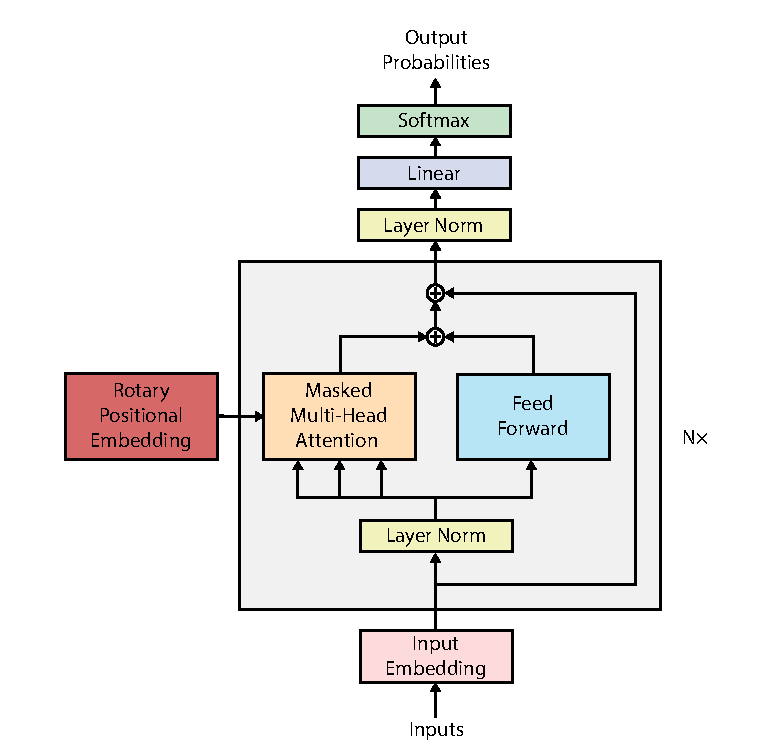
\includegraphics[width=0.8\textwidth]{figures/gpt-j_architecture.pdf}
    \caption{Diagram of GPT-J model architecture}
    \label{fig:gpt-j-architecture}
\end{figure}

\subsection{Requirements}
\label{sec:requirements}
To load the GPT-J model in float32 precision, one would need at least 2x the model size of CPU RAM: 1x for the initial weights and another 1x to load the checkpoint. So for just loading the GPT-J model, it would require at least 48GB or CPU RAM. To reduce the memory footprint, one can load the model in half-precision.

GPU needs around 40GB of GPU memory to load the model. For training/fine-tuning the model, it would require significantly more GPU RAM. For example, the Adam optimizer makes four copies of the model: model, gradients, average and the squared average of gradients. Hence, it would take 4x model size GPU memory, even with mixed precision as gradient updates are in fp32. Further, this doesn't include the activations and data batches which would require some more GPU RAM. Hence, solutions like DeepSpeed needs to be used for training/fine-tuning such large models.

If a GPU with mixed precision capabilities (architecture Pascal or more recent) is available, one can use mixed precision training with PyTorch 1.6.0 or later, or by installing the Apex library for previous versions. If using an NVIDIA “Ampere” GPU architecture, the Brain Floting Point (BF16) floating-point format can be used. Using mixed precision training usually results in 2x-speedup for training with the same final results.

\subsection{Pre-training}
\label{sec:pretraining}
Pre-training is defined as "Training in advanced". By first training the model on a huge dataset, the model can then be fine-tuned on a much smaller dataset. This is so-called transfer learning. In this project, pre-trained weights for GPT-J-6B from ElutherAI are used. The pre-training by ElutherAI is done on the dataset The Pile, described in \cref{sec:the-pile}. Of the roughly 825GiB, 95.16 GiB (7.59\%) of The Pile is code from GitHub. Compared to many other open-source models, GPT-J-6B is one of the most promising models for the task of code generation.

The specific GPT-J model configuration can be seen in \cref{tab:gpt-j-model-details}. In detail, GPT-J-6B consists of 28 layers with a model dimension of 4096, and a feedforward dimension of 16384. The model dimension is split into 16 heads, each with a dimension of 256. \acrfull{rope} is applied to 64 dimensions of each head. The model is trained with a tokenization vocabulary of 50257, using the same set of \acrfullpl{bpe} as GPT-2 and GPT-3. The weights of GPT-J-6B are licensed under version 2.0 of the Apache License.


%Total params: 6,050,882,784
%multi-layer perceptron (MLP)

\begin{table}
    %\newcolumntype{Y}{>{\centering\arraybackslash}X}
    \def\arraystretch{1.5}
    \small
    \centering
    \caption{GPT-J-6B model details.}
    \label{tab:gpt-j-model-details}
    \begin{tabularx}{\textwidth}{XX}
        \toprule
        \textbf{Hyper parameter} & \textbf{Value}\\
        \midrule
        n\_parameters & 6,053,381,344\\
        n\_layers & 28*\\
        d\_model & 4,096\\
        d\_ff & 16,384\\
        n\_heads & 16\\
        d\_head & 256\\
        n\_ctx & 2,048\\
        n\_vocab & 50,257 (same tokenizer as GPT-2/3)\\
        position \& encoding & \acrfullpl{rope}\\
        RoPE dimensions & 64\\
        \bottomrule
    \end{tabularx}
\end{table}

\todo{add table notes}
* each layer consists of one feedforward block and one self attention block


\subsection{Fine-tuning}
\label{sec:fine-tuning}
To improve the pre-trained GPT-J-6B model's smart contract code generation performance, the model is fine-tuned on a dataset only containing real Ethereum Smart Contract code. Specifically, two models are created. The first model, named GPT-J-6B-Smart-Contract, is fine-tuned on the Verified Smart Contracts dataset \cref{sec:verified-smart-contracts}. The other model, named GPT-J-6B-Smart-Contract-Audit, is a secure version of the first model. It is fine-tuned on the Verified Smart Contracts Audit dataset \cref{sec:verified-smart-contracts-audit}, the same dataset as for the first model but with additional labeling from vulnerability analysis.

\begin{table}
    %\newcolumntype{Y}{>{\centering\arraybackslash}X}
    \def\arraystretch{1.5}
    \small
    \centering
    \caption{Hyper parameters for GPT-J model}
    \label{tab:inclusion-exclusion-criteria}
    \begin{tabularx}{\textwidth}{XX}
        \toprule
        \textbf{Hyper parameter} & \\
        \midrule
        \_name\_or\_path & EleutherAI/gpt-j-6B\\
        activation\_function & gelu\_new\\
        architectures & GPTJForCausalLM\\
        attn\_pdrop & 0.0\\
        bos\_token\_id & 50256\\
        embd\_pdrop & 0.0\\
        eos\_token\_id & 50256\\
        gradient\_checkpointing & false\\
        initializer\_range & 0.02\\
        layer\_norm\_epsilon & 1e-05\\
        model\_type & gptj\\
        n\_embd & 4096\\
        n\_head & 16\\
        n\_inner & null\\
        n\_layer & 28\\
        n\_positions & 2048\\
        resid\_pdrop & 0.0\\
        rotary & true\\
        rotary\_dim & 64\\
        scale\_attn\_weights & true\\
        summary\_activation & null\\
        summary\_first\_dropout & 0.1\\
        summary\_proj\_to\_labels & true\\
        summary\_type & cls\_index\\
        summary\_use\_proj & true\\
        tie\_word\_embeddings & false\\
        tokenizer\_class & "GPT2Tokenizer"\\
        transformers\_version & "4.19.0.dev0"\\
        use\_cache & true\\
        vocab\_size & 50400\\
        \bottomrule
    \end{tabularx}
\end{table}


\begin{table}
    %\newcolumntype{Y}{>{\centering\arraybackslash}X}
    \def\arraystretch{1.5}
    \small
    \centering
    \caption{DeepSpeed Zero config.}
    \label{tab:inclusion-exclusion-criteria}
    \begin{tabularx}{\textwidth}{XX}
        \toprule
        \textbf{Hyper parameter} & \\
        \midrule
        stage & 2\\
        contiguous\_gradients & true\\
        reduce\_scatter & true\\
        reduce\_bucket\_size & 2.000000e+08\\
        allgather\_partitions & true\\
        allgather\_bucket\_size & 2.000000e+08\\
        overlap\_comm & true\\
        load\_from\_fp32\_weights & true\\
        elastic\_checkpoint & false\\
        offload\_param & null\\
        \midrule
        offload\_optimizer & device: null\\
        & nvme\_path: null\\
        & buffer\_count: 4\\
        & pin\_memory: false\\
        & pipeline\_read: false\\
        & pipeline\_write: false\\
        & fast\_init: false\\
        \midrule
        sub\_group\_size & 1.000000e+09\\
        prefetch\_bucket\_size & 5.000000e+07\\
        param\_persistence\_threshold & 1.000000e+05\\
        max\_live\_parameters & 1.000000e+09\\
        max\_reuse\_distance & 1.000000e+09\\
        gather\_16bit\_weights\_on\_model\_save & false\\
        ignore\_unused\_parameters & true\\
        round\_robin\_gradients & false\\
        legacy\_stage1 & false\\
        \bottomrule
    \end{tabularx}
\end{table}

\subsection{Inference}

TODO: What is supported by the model? How much memory to use?
We perform beam search with width of 5 and optimize for accuracy@1


\subsection{Security Conditioning}
\label{sec:security-conditioning}
When training a large language model on several gigabytes of open-source code, it is safe to assume that large portions of this code are not safe and contains vulnerabilities. In the case of Smart Contracts, the vulnerability analysis presented in section \ref{sec:verified-smart-contracts} shows that almost 50\% of deployed Smart Contracts contain at least one high-severity vulnerability. This will result in a biased model that may produce a lot of vulnerable code. This section introduces a technique, named security conditioning, to reduce and mitigate this problem.

Vulnerability analysis is a difficult area. It is especially hard in the area of smart contracts, where the execution environment is not deterministic ????\todo{find correct wording.}... Previous works have tried to classify vulnerable code with large language models without much success \todo{Cite previous works}. In this project, instead of classifying vulnerable code, the goal is to make the model more secure by conditioning it on the presence of vulnerabilities.

The security conditioning is done by appending a special security label to each of the records in the training data. This way, the model can use this token(s) to condition whether to produce safe or vulnerable code. This requires the dataset to first be labeled as secure or vulnerable. For this project, SolidityDetector is used for labeling. Further details on the dataset construction can be found in \cref{sec:verified-smart-contracts-audit}.

\todo{Add example of security conditioning.}
%\input{chapters/x-data.tex}
%\chapter{Language Modeling}
\label{chap:language-modeling}
This chapter presents the results of this thesis. The chapter starts with ... the research questions defined in \cref{sec:research-questions}.

As discussed in section \cref{sec:transformers-for-code-synthesis}, there are several available transformer models. However, only a few of them have open-sourced pre-trained weights. Of these, only GPT-J \cite{gpt-j} includes code in it's pre-training dataset "The Pile", described in \cref{sec:the-pile}. As GPT-J is a state-of-the-art generative pre-trained transformer model, this is the language model used in this thesis. This chapter presents a detailed overview of the system architecture for generating secure Smart Contract code. The first section gives an overview of the GPT-J model architecture, followed by a section describing the pre-training of the model. The third section describes the fine-tuning process on the smart contract dataset presented in \cref{sec:verified-smart-contracts-inflated,sec:verified-smart-contracts-audit}. 

\todo{Add figure of training process}

\section{Model architecture}
\label{sec:architecture}
Ever since OpenAI introduced its first transformer model in the GPT series, this class of transformers has been touted as the state-of-the-art for text generation. Their latest model, GPT-3 \cite{brown2020language}, is their best performing model with 175 billion parameters. However, the model is not openly available at the current time. GPT-J \cite{gpt-j} with 6 billion parameters (GPT-J-6B) is currently one of the best open-source alternatives to OpenAI's GPT-3. GPT-J was released in June 2021 by EleutherAI \cite{elutherai}, a grassroots collection of researchers working to open-source AI research. The model is trained on the Pile, an 825 GiB diverse, open-source language modeling data set that consists of 22 smaller, high-quality datasets combined together. See section \cref{sec:the-pile} for a more detailed description of the Pile.

Being a GPT class transformer, GPT-J uses a decoder-only architecture, as can be seen in \cref{fig:gpt-j-architecture}. The GPT-J introduces some notable differences from standard transformer models. Firstly, instead of computing attention and feed-forward layers in sequential order, they are computed in parallel and the results are added together. This decreases communication during distributed training, resulting in increased throughput. Secondly, GPT-J uses \acrfull{rope} \cite{su2021roformer} for position encoding. Opposite to sinusoidal encoding used in standard transformer models (see \cref{sec:embedding-and-positional-encoding}), this is shown to result in better model quality in tasks with long text \cite{su2021roformer}.

\begin{figure}[htp]
    \centering
    %\def\svgwidth{\linewidth}
    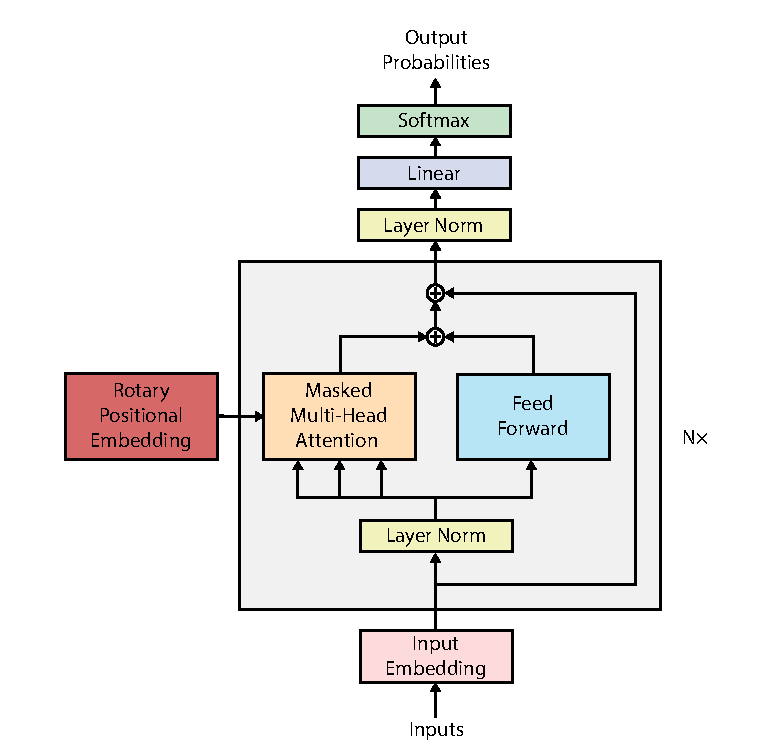
\includegraphics[width=0.8\textwidth]{figures/gpt-j_architecture.pdf}
    \caption{Diagram of GPT-J model architecture}
    \label{fig:gpt-j-architecture}
\end{figure}

\section{Requirements}
\label{sec:requirements}
To load the GPT-J model in float32 precision, one would need at least 2x the model size of CPU RAM: 1x for the initial weights and another 1x to load the checkpoint. So for just loading the GPT-J model, it would require at least 48GB or CPU RAM. To reduce the memory footprint, one can load the model in half-precision.

GPU needs around 40GB of GPU memory to load the model. For training/fine-tuning the model, it would require significantly more GPU RAM. For example, the Adam optimizer makes four copies of the model: model, gradients, average and the squared average of gradients. Hence, it would take 4x model size GPU memory, even with mixed precision as gradient updates are in fp32. Further, this doesn't include the activations and data batches which would require some more GPU RAM. Hence, solutions like DeepSpeed needs to be used for training/fine-tuning such large models.

If a GPU with mixed precision capabilities (architecture Pascal or more recent) is available, one can use mixed precision training with PyTorch 1.6.0 or later, or by installing the Apex library for previous versions. If using an NVIDIA “Ampere” GPU architecture, the Brain Floting Point (BF16) floating-point format can be used. Using mixed precision training usually results in 2x-speedup for training with the same final results.

\section{Pre-training}
\label{sec:pretraining}
Pre-training is defined as "Training in advanced". By first training the model on a huge dataset, the model can then be fine-tuned on a much smaller dataset. This is so-called transfer learning. In this project, pre-trained weights for GPT-J-6B from ElutherAI are used. The pre-training by ElutherAI is done on the dataset The Pile, described in \cref{sec:the-pile}. Of the roughly 825GiB, 95.16 GiB (7.59\%) of The Pile is code from GitHub. Compared to many other open-source models, GPT-J-6B is one of the most promising models for the task of code generation.

The specific GPT-J model configuration can be seen in \cref{tab:gpt-j-model-details}. In detail, GPT-J-6B consists of 28 layers with a model dimension of 4096, and a feedforward dimension of 16384. The model dimension is split into 16 heads, each with a dimension of 256. \acrfull{rope} is applied to 64 dimensions of each head. The model is trained with a tokenization vocabulary of 50257, using the same set of \acrfullpl{bpe} as GPT-2 and GPT-3. The weights of GPT-J-6B are licensed under version 2.0 of the Apache License.


%Total params: 6,050,882,784
%multi-layer perceptron (MLP)

\begin{table}
    %\newcolumntype{Y}{>{\centering\arraybackslash}X}
    \def\arraystretch{1.5}
    \small
    \centering
    \caption{GPT-J-6B model details.}
    \label{tab:gpt-j-model-details}
    \begin{tabularx}{\textwidth}{XX}
        \toprule
        \textbf{Hyper parameter} & \textbf{Value}\\
        \midrule
        n\_parameters & 6,053,381,344\\
        n\_layers & 28*\\
        d\_model & 4,096\\
        d\_ff & 16,384\\
        n\_heads & 16\\
        d\_head & 256\\
        n\_ctx & 2,048\\
        n\_vocab & 50,257 (same tokenizer as GPT-2/3)\\
        position \& encoding & \acrfullpl{rope}\\
        RoPE dimensions & 64\\
        \bottomrule
    \end{tabularx}
\end{table}

\todo{add table notes}
* each layer consists of one feedforward block and one self attention block


\section{Fine-tuning}
\label{sec:fine-tuning}
To improve the pre-trained GPT-J-6B model's smart contract code generation performance, the model is fine-tuned on a dataset only containing real Ethereum Smart Contract code. Specifically, two models are created. The first model, named GPT-J-6B-Smart-Contract, is fine-tuned on the Verified Smart Contracts dataset \cref{sec:verified-smart-contracts}. The other model, named GPT-J-6B-Smart-Contract-Audit, is a secure version of the first model. It is fine-tuned on the Verified Smart Contracts Audit dataset \cref{sec:verified-smart-contracts-audit}, the same dataset as for the first model but with additional labeling from vulnerability analysis.

\begin{table}
    %\newcolumntype{Y}{>{\centering\arraybackslash}X}
    \def\arraystretch{1.5}
    \small
    \centering
    \caption{Hyper parameters for GPT-J model}
    \label{tab:inclusion-exclusion-criteria}
    \begin{tabularx}{\textwidth}{XX}
        \toprule
        \textbf{Hyper parameter} & \\
        \midrule
        \_name\_or\_path & EleutherAI/gpt-j-6B\\
        activation\_function & gelu\_new\\
        architectures & GPTJForCausalLM\\
        attn\_pdrop & 0.0\\
        bos\_token\_id & 50256\\
        embd\_pdrop & 0.0\\
        eos\_token\_id & 50256\\
        gradient\_checkpointing & false\\
        initializer\_range & 0.02\\
        layer\_norm\_epsilon & 1e-05\\
        model\_type & gptj\\
        n\_embd & 4096\\
        n\_head & 16\\
        n\_inner & null\\
        n\_layer & 28\\
        n\_positions & 2048\\
        resid\_pdrop & 0.0\\
        rotary & true\\
        rotary\_dim & 64\\
        scale\_attn\_weights & true\\
        summary\_activation & null\\
        summary\_first\_dropout & 0.1\\
        summary\_proj\_to\_labels & true\\
        summary\_type & cls\_index\\
        summary\_use\_proj & true\\
        tie\_word\_embeddings & false\\
        tokenizer\_class & "GPT2Tokenizer"\\
        transformers\_version & "4.19.0.dev0"\\
        use\_cache & true\\
        vocab\_size & 50400\\
        \bottomrule
    \end{tabularx}
\end{table}


\begin{table}
    %\newcolumntype{Y}{>{\centering\arraybackslash}X}
    \def\arraystretch{1.5}
    \small
    \centering
    \caption{DeepSpeed Zero config.}
    \label{tab:inclusion-exclusion-criteria}
    \begin{tabularx}{\textwidth}{XX}
        \toprule
        \textbf{Hyper parameter} & \\
        \midrule
        stage & 2\\
        contiguous\_gradients & true\\
        reduce\_scatter & true\\
        reduce\_bucket\_size & 2.000000e+08\\
        allgather\_partitions & true\\
        allgather\_bucket\_size & 2.000000e+08\\
        overlap\_comm & true\\
        load\_from\_fp32\_weights & true\\
        elastic\_checkpoint & false\\
        offload\_param & null\\
        \midrule
        offload\_optimizer & device: null\\
        & nvme\_path: null\\
        & buffer\_count: 4\\
        & pin\_memory: false\\
        & pipeline\_read: false\\
        & pipeline\_write: false\\
        & fast\_init: false\\
        \midrule
        sub\_group\_size & 1.000000e+09\\
        prefetch\_bucket\_size & 5.000000e+07\\
        param\_persistence\_threshold & 1.000000e+05\\
        max\_live\_parameters & 1.000000e+09\\
        max\_reuse\_distance & 1.000000e+09\\
        gather\_16bit\_weights\_on\_model\_save & false\\
        ignore\_unused\_parameters & true\\
        round\_robin\_gradients & false\\
        legacy\_stage1 & false\\
        \bottomrule
    \end{tabularx}
\end{table}

\section{Inference}

TODO: What is supported by the model? How much memory to use?
We perform beam search with width of 5 and optimize for accuracy@1


\section{Security Conditioning}
\label{sec:security-conditioning}
When training a large language model on several gigabytes of open-source code, it is safe to assume that large portions of this code are not safe and contains vulnerabilities. In the case of Smart Contracts, the vulnerability analysis presented in section \ref{sec:verified-smart-contracts} shows that almost 50\% of deployed Smart Contracts contain at least one high-severity vulnerability. This will result in a biased model that may produce a lot of vulnerable code. This section introduces a technique, named security conditioning, to reduce and mitigate this problem.

Vulnerability analysis is a difficult area. It is especially hard in the area of smart contracts, where the execution environment is not deterministic ????\todo{find correct wording.}... Previous works have tried to classify vulnerable code with large language models without much success \todo{Cite previous works}. In this project, instead of classifying vulnerable code, the goal is to make the model more secure by conditioning it on the presence of vulnerabilities.

The security conditioning is done by appending a special security label to each of the records in the training data. This way, the model can use this token(s) to condition whether to produce safe or vulnerable code. This requires the dataset to first be labeled as secure or vulnerable. For this project, SolidityDetector is used for labeling. Further details on the dataset construction can be found in \cref{sec:verified-smart-contracts-audit}.

\todo{Add example of security conditioning.}
% Or call it Research results?

\chapter{Research Implementation and Results}
\label{chap:implementation-and-results}
This chapter presents the research implementation and results of the research questions. The chapter is divided into two parts. First, the implementation of research question 1 is described, concerning automatic smart contract code synthesis. The part of the chapter describes the implementation of research question 2, regarding generating secure smart contract code.

\section{Implementation of RQ1}
This section presents the implementation of research question 1. The implementation is done with the following steps:
\begin{enumerate}
    \item Create verified smart contract source code dataset.
    \begin{enumerate}
        \item Scrape verified smart contracts from the Ethereum blockchain.
        \item Normalize the smart contract files.
        \item Filter the smart contracts for uniqueness.
    \end{enumerate}
    \item Code comment analysis.
    \begin{enumerate}
        \item Create a parser that can parse all contract versions.
        \item Parse verified smart contract source code.
        \item Create a parsed dataset containing "comment, function" pairs.
        \item Cluster comments.
    \end{enumerate}
    \item Language modeling
    \begin{enumerate}
        \item Fine-tune a transformer model on the verified smart contracts dataset.
    \end{enumerate}
\end{enumerate}

\subsection{Data collection}
\label{sec:data-collection}

\subsubsection{Smart contract downloader}
\label{sec:smart-contract-downloader}

The largest provider of verified \acrshortpl{sc} is Etherscan. At \url{https://etherscan.io/} users can upload the source code for their deployed \acrshort{sc}. Etherscan will then compile this source code and verify that it matches the bytecode of the deployed \acrshort{sc} on the Ethereum blockchain. This way, other people can verify the functionality of a \acrshort{sc} before using it. Etherscan provides a simple \acrshort{api} for downloading verified Smart Contracts. The API is available at \url{https://api.etherscan.io/api}. From this endpoint, one can ask for the verified source code of a specific \acrshort{sc} address. However, it is not guaranteed that the contract has been verified.

The following code snippet is a Google BigQuery query. It selects all \acrshortpl{sc} addresses on the Ethereum blockchain that has at least one transaction. This query was run on the 1st of April 2022, and the result was downloaded as a CSV file, available on request at \url{https://huggingface.co/datasets/andstor/smart_contracts/blob/main/contract_addresses.csv}. The CSV file is then used to download the \acrshortpl{sc} from Etherscan.

\begin{lstlisting}[
    caption={Google BigQuery query for selecting all \acrlong{sc} addresses on Ethereum that has at least one transaction.},
    label=lst:reentrancy,
    language=SQL]
SELECT contracts.address, COUNT(1) AS tx_count
FROM `bigquery-public-data.crypto_ethereum.contracts` AS contracts
JOIN `bigquery-public-data.crypto_ethereum.transactions` AS transactions 
      ON (transactions.to_address = contracts.address)
GROUP BY contracts.address
ORDER BY tx_count DESC
\end{lstlisting}

%Saved to file for simple restarting, multiprocessing and parallelization.

The total number of files generated by the downloading program (\url{https://github.com/andstor/smart-contract-downloader}) was 5,810,042. In order to efficiently process these, all files were combined into a tarfile. A processing script was then created for filtering out all "empty" files. These correspond to a contract address on Ethereum that has not been verified on Etherscan.io. A total of 3,592,350 files were empty, making the source code of 38,17\% of the deployed contracts on Ethereum available. Each non-empty file is then parsed and the contract data is extracted. This extraction process is rather complicated, as smart contract sources come in a wide variety of flavors and formats. 

\paragraph{Normalization of smart contract files}
\label{par:normalization}
\acrshortpl{sc} come in multiple flavors. To avoid confusing the machine learning model, all training data should use the same format. Hence, all contract files are normalized. The most common format is a contract written the Solidity language with a single contract entry in the file. However, a single contract file can contain multiple contracts, making use of properties like inheritance etc. The source code contracts can also be split over multiple files, a format referred to as "Multi file". When compiling these, the source code files are "flattened" into a single contract file before compilation. Another flavor is the JSON format, which is a language that is used to describe the \acrshortpl{sc}. As can be seen in \cref{lst:standard-json-format}, here the source code is structured inside JSON code. Smart contracts can also be written in the Vyper language. Vyper is Pythonic programming language. Compared to Solidity, it has deliberately fewer features, making contracts more secure and easier to edit \cite{vyper}. However, it is much less popular than Solidity.

\begin{lstlisting}[
    caption={Solidity standard JSON Input format.},
    label=lst:standard-json-format,
    language=JSON]
{
    "sources": {/* ... */},
    "settings": {
        "optimizer": {/* ... */},
        "evmVersion": "<VERSION>"
    }
}
\end{lstlisting}

All of the above formats are processed by the processing script, normalizing the contract source code to a single "flattened" contract file. The source code, along with the contract metadata, is then saved across multiple Parquet files, each consisting of 30000 "flattened" contracts. A total of 2,217,692 smart contracts were successfully parsed and normalized.

\paragraph{Filter smart contracts for uniqueness}
\label{sec:duplication-filtering}
A large quantity of Smart Contracts contains duplicated code. Primarily, this is due to the frequent use of library code, such as SafeMath \cite{safemath} by OpenZeppelin \cite{openzeppelin}. Etherscan requires the library code used in a contract to be embedded in the source code. Filtering is applied to produce a dataset with a mostly unique contract source code to mitigate this. This is very important when used for model training. Failure to produce a sufficiently unique dataset would result in poor performance of a machine learning model, as it would overfit on similar data. The filtering is done by calculating the string distance between the source code. Due to the rather large amount of contracts (\~2 million), the comparison is only made within groups of contracts. These groups are defined by grouping on the "contract\_name" for the \textit{flattened} dataset, and by "file\_name" for the \textit{inflated} dataset. These datasets will be discussed in detail in the following sections.

The actual code filtering is done by applying a token-based similarity algorithm named Jacard Index, described in \cref{sec:jaccard-index}. The algorithm is computationally efficient and can be used to filter out \acrshortpl{sc} that are not similar to the query.

\subsubsection{Verified Smart Contracts}
\label{sec:verified-smart-contracts}
The Verified Smart Contracts dataset is a dataset consisting of verified Smart Contracts from Etherscan.io. These are real \acrshortpl{sc} that are deployed to the Ethereum blockchain, containing primarily Solidity and a very small fraction Vyper code. The dataset contains multiple subsets. In the following paragraphs, these subsets are described in detail. It consists of every deployed Ethereum Smart Contract as of 1st of April 2022, whose been verified on Etherescan.io and has a least one transaction. \cref{tab:verified-smart-contracts-metrics} shows the metrics of the various subsets. All processing scripts are available at \url{https://github.com/andstor/verified-smart-contracts}. The dataset is available on request at \url{https://huggingface.co/datasets/andstor/verified-smart-contracts}.

\begin{table}
    %\newcolumntype{Y}{>{\centering\arraybackslash}X}
    \def\arraystretch{1.5}
    \small
    \centering
    \caption{Verified Smart Contracts Metrics}
    \label{tab:verified-smart-contracts-metrics}
    \begin{tabularx}{\textwidth}{XXXX}
        \toprule
        \textbf{Component} & \textbf{Size} &  \textbf{Num rows} & \textbf{\acrshort{loc}}\\
        \midrule
        Raw & 0.80 GiB & 2,217,692 & 839,665,295\\
        Flattened & 1.16 GiB & 136,969 & 97,529,473\\
        Inflated & 0.76 GiB & 186,397 & 53,843,305\\
        \bottomrule
    \end{tabularx}
\end{table}

\paragraph{Raw}
\label{sec:verified-smart-contracts-raw}
The raw dataset contains mostly the raw data from Etherscan, downloaded with the smart-contract-downlader tool, as described in \cref{sec:smart-contract-downloader}. All different contract formats (JSON, multi-file, etc.) are normalized to a flattened source code structure, as described in \cref{par:normalization}.

\paragraph{Flattened}
\label{sec:verified-smart-contracts-flattened}

The flattened dataset is a filtered version of the Raw dataset. It contains smart contracts, where every contract contains all required library code. Each "file" is marked in the source code with a comment stating the original file path: //File: path/to/file.sol. These are then filtered for uniqueness with a similarity threshold of 0.9,  calculated using the Jacard index. This means that all contracts whose code shares more than 90\% of the tokens will be discarded. The low uniqueness requirement is due to the often large amount of embedded library code. If the requirement is set to high, the actual contract code will be negligible compared to the library code. Most contracts will be discarded, and the resulting dataset would contain mostly unique library code. However, the dataset as a whole will have a large amount of duplicated library code. From the 2,217,692 contracts, 2,080,723 duplications are found, giving a duplication percentage of 93.82\%. The resulting dataset consists of 136,969 contracts. \cref{lst:flattened-dataset-instance} shows an example data instance from the dataset. The dataset is then split 80\%, 10\%, 10\% into a training, validation and test set, respectively.

%Processing: 100%|██████| 74/74 [20:22<00:00, 16.51s/it, dupes=2081081/2217692 (93.84%)]
%
%The following command prooduces the flattened dataset:
%
%\lstinline[language=Python]!python script/filter_data.py -s parquet -o data/flattened --threshold 0.9!


\begin{lstlisting}[
    float,floatplacement=H!,
    caption={Example data instance from the flattened dataset.},
    label=lst:flattened-dataset-instance,
    language=JSON]
{
  'contract_name': 'MiaKhalifaDAO',
  'contract_address': '0xb3862ca215d5ed2de22734ed001d701adf0a30b4',
  'language': 'Solidity',
  'source_code': '// File: @openzeppelin/contracts/utils/Strings.sol\r\n\r\n\r\n// OpenZeppelin Contracts v4.4.1 (utils/Strings.sol)\r\n\r\npragma solidity ^0.8.0;\r\n\r\n/**\r\n * @dev String operations.\r\n */\r\nlibrary Strings {\r\n...',
  'abi': '[{"inputs":[{"internalType":"uint256","name":"maxBatchSize_","type":"uint256"}...]',
  'compiler_version': 'v0.8.7+commit.e28d00a7',
  'optimization_used': False,
  'runs': 200,
  'constructor_arguments': '000000000000000000000000000000000000000000000000000000000000000a000...',
  'evm_version': 'Default',
  'library': '',
  'license_type': 'MIT',
  'proxy': False,
  'implementation': '',
  'swarm_source': 'ipfs://e490df69bd9ca50e1831a1ac82177e826fee459b0b085a00bd7a727c80d74089'
}
\end{lstlisting}

\paragraph{Inflated}
\label{sec:verified-smart-contracts-inflated}
The inflated dataset is also based on the raw dataset. Each contract file in the dataset is split into its original representative files and hence  "inflated". This mitigates a lot of the problems of the flattened dataset in terms of duplicated library code. The library code is, along with other imported contract files, split (read inflated) into separate contract records. The 2,217,692 "raw" smart contracts are inflated to a total of 5,403,136 separate contract files. These are then grouped by "file\_name" and filtered for uniqueness with a similarity threshold of 0.9. This should produce a dataset with a large amount of unique source code, with low quantities of library code. A total of 5,216,739 duplications are found, giving a duplication percentage of 96.56\%. The resulting dataset consists of 186,397 contracts. \cref{lst:inflated-dataset-instance} shows an example data instance from the inflated dataset. The dataset is then split 80\%, 10\%, 10\% into a training, validation and test set, respectively.

%Processing: 100%|██████| 74/74 [22:50<00:00, 18.52s/it, dupes=5217191/5403136 (96.56%)]


%\lstinline[language=Python]!python script/filter_data.py -s parquet -o data/inflated --split-files --threshold 0.9!
%dupes=5217191/5403136 (96.56%)


\begin{lstlisting}[
    float,floatplacement=H!,
    caption={Example data instance from the inflated dataset.},
    label=lst:inflated-dataset-instance,
    language=JSON]
{
    'contract_name': 'PinkLemonade',
    'file_path': 'PinkLemonade.sol',
    'contract_address': '0x9a5be3cc368f01a0566a613aad7183783cff7eec',
    'language': 'Solidity',
    'source_code': '/**\r\n\r\nt.me/pinklemonadecoin\r\n*/\r\n\r\n// SPDX-License-Identifier: MIT\r\npragma solidity ^0.8.0;\r\n\r\n\r\n/*\r\n * @dev Provides information about the current execution context, including the\r\n * sender of the transaction and its data. While these are generally available...',
    'abi': '[{"inputs":[],"stateMutability":"nonpayable","type":"constructor"}...]',
    'compiler_version': 'v0.8.4+commit.c7e474f2',
    'optimization_used': False,
    'runs': 200,
    'constructor_arguments': '',
    'evm_version': 'Default',
    'library': '',
    'license_type': 'MIT',
    'proxy': False,
    'implementation': '',
    'swarm_source': 'ipfs://eb0ac9491a04e7a196280fd27ce355a85d79b34c7b0a83ab606d27972a06050c'
}
\end{lstlisting}

\paragraph{Plain text}
\label{sec:verified-smart-contracts-plain-text}
For easy use of the dataset for casual language modeling training with HuggingFace, a "plain\_text" version of both the raw, the flattened, and the inflated dataset is made available. This is done through a custom builder script for the dataset, a feature of the Dataset library by Hugging Face. \cref{lst:inflated-dataset-instance-plain-text} shows an example data instance of the "plain\_text" version.


\begin{lstlisting}[
    caption={Example data instance from the plain-text version of the inflated dataset.},
    label=lst:inflated-dataset-instance-plain-text,
    language=JSON]
{
    'language': 'Solidity',
    'text': 'pragma solidity =0.5.16;\r\n\r\n// a library for performing overflow-safe math...'
}
\end{lstlisting}

%\todo{fix tokens}
%smart\_contracts\_dataset :: inflated\_plain\_text tokens:
%	test: 74314082
%	validation: 67064318
%	train: 687186308
%TOTAL: 828.564.708

\FloatBarrier

\subsection{Code comment analysis}
\label{sec:comment-analysis}
To provide some insight into how a user can best formulate a comment for guiding the code synthesis, a cluster analysis of the comments in the smart contract dataset is conducted. First, a universal Solidity parser is constructed for parsing the Solidity code and extracting "code, comment" pairs. These results are then packaged into a dataset, and a clustering analysis is conducted. The results from this analysis are then later used in the evaluation of the code synthesis in \cref{chap:evaluation} to shedd some light on which commenting style is the best to use.

\subsubsection{Universal Solidity parser}
\label{sec:universal-solidity-parser}
To parse the Solidity \acrshort{sc}, a Solidity parser is constructed. This parser has to be universally compatible with all Solidity versions, hence the grammar used needs to be a lot less restrictive than the current official Solidity grammar available from Ethereum \cite{soliditygrammar}. ANTLR4 \cite{antlr4} is used for constructing the parser. ANTLR is a parser generator. By providing ANTLR with a formal language description called grammar, it can generate a complete parser that can automatically build parse trees. Parse trees are data structures representing how the grammar matches the input. Specifically, ANTLR4 generates a LL(*) (Left-to-right, leftmost derivation) parser \cite{parr2011llstar}. ANTLR is primarily a Java application. However, several code generation targets are available, including Java, C\#, Python, JavaScript, Go, C++, Swift, PHP and Dart \cite{antlr-targets}. In this project, the Python target is used.

Most programming language grammars available do not devote much effort to the handling of code comments. Comments are seen as unnecessary clutter and are normally discarded during lexing. For extracting the comments from the Solidity \acrshort{sc} code, the original source \cite{solidity-antlr4} for the official Solidity grammar \cite{soliditygrammar} is used. This old version is less restrictive and serves as a better starting point for ensuring support for all Solidity versions. This grammar is then simplified and made less restrictive, as well as adapted to support comments. \cref{fig:solidity-railroad-diagram} shows a railroad diagram of a subset of the main grammar rules altered for supporting comments. The complete universal Solidity parser is made available at https://github.com/andstor/solidity-universal-parser.

\begin{figure}[htbp]
    \centering
    %\makebox[\textwidth][c]{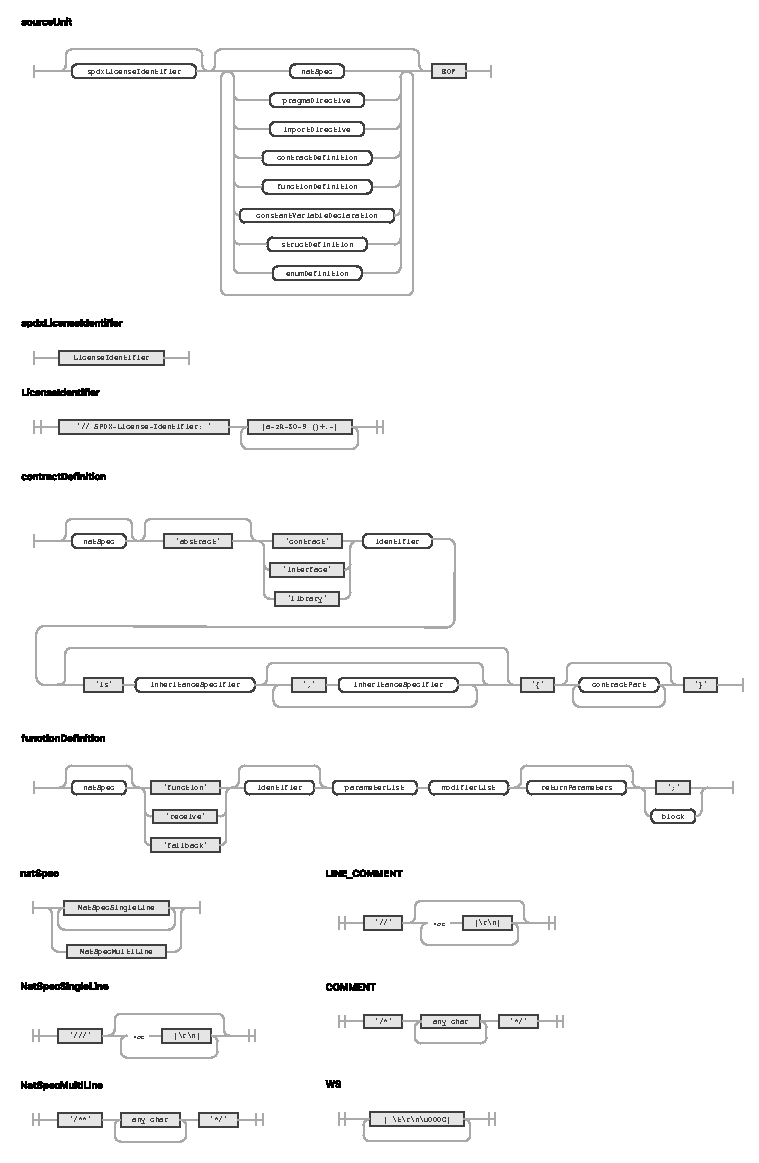
\includegraphics{figures/solidity-comments-railroad-diagram.pdf}}%
    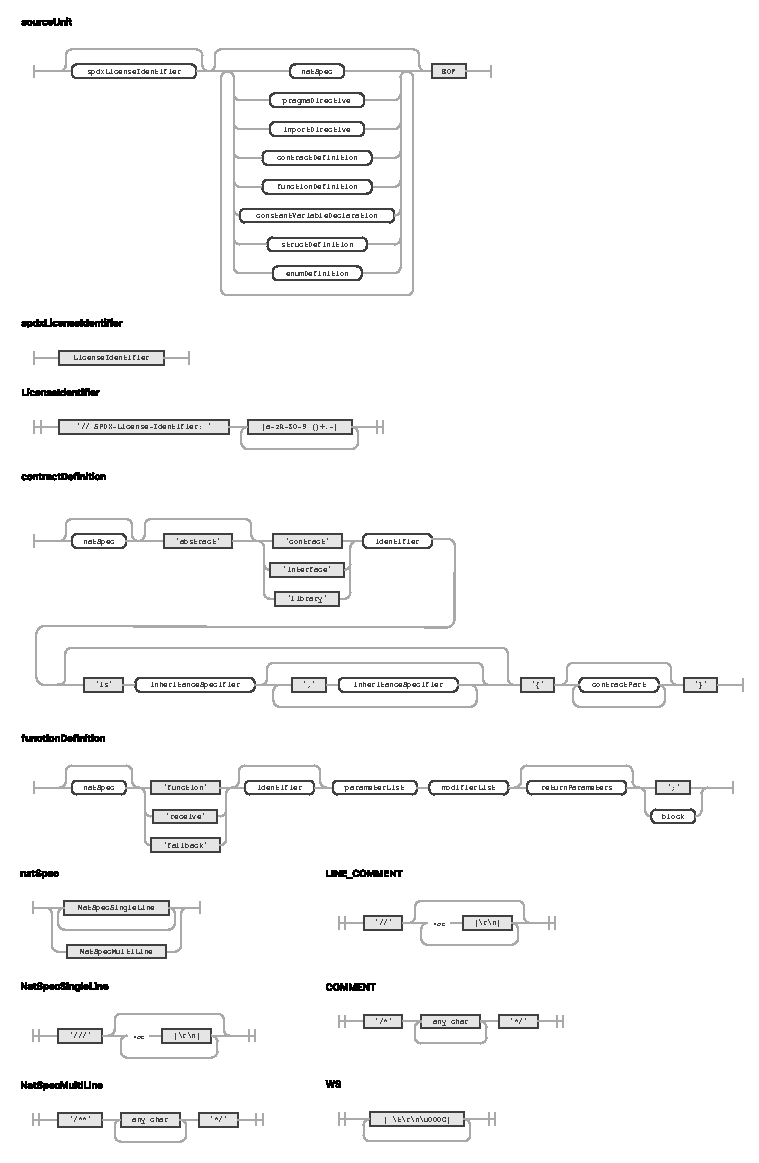
\includegraphics[width=\textwidth]{figures/solidity-comments-railroad-diagram.pdf}
    \caption{Railroad diagrams of main code comment alteration to Solidity grammar.}
    \label{fig:solidity-railroad-diagram}
\end{figure}


\subsubsection{Verified Smart Contract Code Comments}
\label{sec:verified-smart-contract-code-comments}
For doing the actual extraction of the "code, comment" pairs from the inflated version of the Verified Smart Contracts dataset (see \cref{sec:verified-smart-contracts-inflated}), the well-known visitor pattern \cite{visitor-pattern} is used for visiting the parse tree generated by the universal Solidity parser. ANTLER provides basic infrastructure for implementing such a visitor. The full implementation of the visitor is available at \url{https://github.com/andstor/verified-smart-contracts/blob/main/script/comment_visitor.py}. A script leveraging multiprocessing is used to parallelize the parsing of the dataset. See \url{https://github.com/andstor/verified-smart-contracts} for instructions on how to use this script. The resulting data is then filtered for functions that do not have code comments. These are simply removed and the result is then packaged as a new dataset named Verified Smart Contract Code Comments. A total of 1.541.370 functions are extracted. \cref{lst:comments-dataset-instance} shows an example data instance from the dataset. The dataset is available on request at \url{https://huggingface.co/datasets/andstor/smart_contract_comments}.

%The results are then packaged and added to the Verified Smart Contracts dataset collection (\cref{sec:verified-smart-contracts}) under the name "parsed".Verified Smart Contracts dataset collection (\cref{sec:verified-smart-contracts}).

%Parsed: Total 4434014 functions, 4.44 GiB and 29965185 lines of code
%\lstinline[language=Python]!python script/parse_data.py -s data/inflated -o data/parsed!

\begin{lstlisting}[
    float,floatplacement=H!,
    caption={Example data instance from the inflated dataset.},
    label=lst:comments-dataset-instance,
    language=JSON]
{
    'contract_name': 'BondedECDSAKeep',
    'file_path': '@keep-network/keep-core/contracts/StakeDelegatable.sol',
    'contract_address': '0x61935dc4ffc5c5f1d141ac060c0eef04a792d8ee',
    'language': 'Solidity',
    'class_name': 'StakeDelegatable',
    'class_code': 'contract StakeDelegatable {\n    using OperatorParams for uint256;\n\n    mapping(address => Operator) internal operators;\n\n    struct Operator {\n        uint256 packedParams;\n        address owner;\n        address payable beneficiary;\n        address authorizer;\n    }\n\n...',
    'class_documentation': '/// @title Stake Delegatable\n/// @notice A base contract to allow stake delegation for staking contracts.',
    'class_documentation_type': 'NatSpecSingleLine',
    'func_name': 'balanceOf',
    'func_code': 'function balanceOf(address _address) public view returns (uint256 balance) {\n        return operators[_address].packedParams.getAmount();\n    }',
    'func_documentation': '/// @notice Gets the stake balance of the specified address.\n/// @param _address The address to query the balance of.\n/// @return An uint256 representing the amount staked by the passed address.',
    'func_documentation_type': 'NatSpecSingleLine',
    'compiler_version': 'v0.5.17+commit.d19bba13',
    'license_type': 'MIT',
    'swarm_source': 'bzzr://63a152bdeccda501f3e5b77f97918c5500bb7ae07637beba7fae76dbe818bda4'
}  
\end{lstlisting}

\subsubsection{Comment clustering}
\label{sec:comment-clustering}
This section is devoted to the clustering of the comments in the parsed dataset. The comments in the dataset are first preprocessed. In contrast to normal code, code comments are of a more natural language style. Normal natural language text preprocessing is therefore employed. First, the comments are lowercased and tokenized. The default English configuration of the \lstinline[language=Python]!word_tokenize! function from the popular \acrfull{nltk} \cite{nltk} python library is used for tokenization. Stemming is applied to the tokenized words, using the Porter Stemmer algorithm.

For converting the tokenized comments into word embeddings, both the word2vec algorithm \cite{word2vec} and \acrfull{tfidf} is used. The word2vec is able to capture some semantic similarities between the words. In particular, the implementation provided by the gensim library \cite{gensim} is used. The algorithm is configured to produce 100-dimensional vectors, using a window size of 5, and a minimum count of 5. 
%Word2Vec min_count=5,
%                     window=5,
%                     vector_size=100,
%                     sample=0.001,
%                     seed=1,
%                     alpha=0.025,
%                     min_alpha=0.0001, 
%                     negative=5,

To weed out the most frequent words \acrshort{tfidf} is also applied. For example, the different commenting types all start each line with a special word, such as "//", "///" or "*". By using \acrshort{tfidf}, it is possible to get more insights into the different ways of writing comments, beyond just the formatting style of the comments. The resulting word embeddings from the word2vec and \acrshort{tfidf} are multiplied. For each comment, the resulting word embeddings are averaged to form a final comment (or document) embedding.

The comment embeddings are clustered using the K-means algorithm. The number of clusters \(k\) is determined by using the Elbow method for deciding the optimal number of clusters. The results from the Elbow method are presented in \cref{fig:elbow}. From the curve, it is not entirely obvious where the "elbow" is. However, a \(k\) of 4 is selected. For visually inspecting the clustered comments result, the 100-dimensional vectors are reduced to 2D using \acrfull{pca}. The explained variance captured in the 2D plot is approximately 0.64, as shown in the Scree Plot in \cref{fig:scree-plot}. The clustering result is shown in \cref{fig:comment-clusters}.

%Word2Vec lifecycle event {'msg': 'training on 1431483720 raw words (762458270 effective words) took 782.9s, 973910 effective words/s', 'datetime': '2022-06-07T00:40:05.999678', 'gensim': '4.2.0', 'python': '3.7.13 (default, Apr 24 2022, 01:04:09) \n[GCC 7.5.0]', 'platform': 'Linux-5.4.188+-x86_64-with-Ubuntu-18.04-bionic', 'event': 'train'}
%Time to train the model: 13.05 mins

\begin{figure}[htbp]
    \centering
    %% Creator: Matplotlib, PGF backend
%%
%% To include the figure in your LaTeX document, write
%%   \input{<filename>.pgf}
%%
%% Make sure the required packages are loaded in your preamble
%%   \usepackage{pgf}
%%
%% and, on pdftex
%%   \usepackage[utf8]{inputenc}\DeclareUnicodeCharacter{2212}{-}
%%
%% or, on luatex and xetex
%%   \usepackage{unicode-math}
%%
%% Figures using additional raster images can only be included by \input if
%% they are in the same directory as the main LaTeX file. For loading figures
%% from other directories you can use the `import` package
%%   \usepackage{import}
%%
%% and then include the figures with
%%   \import{<path to file>}{<filename>.pgf}
%%
%% Matplotlib used the following preamble
%%
\begingroup%
\makeatletter%
\begin{pgfpicture}%
\pgfpathrectangle{\pgfpointorigin}{\pgfqpoint{4.621007in}{3.063765in}}%
\pgfusepath{use as bounding box, clip}%
\begin{pgfscope}%
\pgfsetbuttcap%
\pgfsetmiterjoin%
\definecolor{currentfill}{rgb}{1.000000,1.000000,1.000000}%
\pgfsetfillcolor{currentfill}%
\pgfsetlinewidth{0.000000pt}%
\definecolor{currentstroke}{rgb}{1.000000,1.000000,1.000000}%
\pgfsetstrokecolor{currentstroke}%
\pgfsetdash{}{0pt}%
\pgfpathmoveto{\pgfqpoint{0.000000in}{0.000000in}}%
\pgfpathlineto{\pgfqpoint{4.621007in}{0.000000in}}%
\pgfpathlineto{\pgfqpoint{4.621007in}{3.063765in}}%
\pgfpathlineto{\pgfqpoint{0.000000in}{3.063765in}}%
\pgfpathclose%
\pgfusepath{fill}%
\end{pgfscope}%
\begin{pgfscope}%
\pgfsetbuttcap%
\pgfsetmiterjoin%
\definecolor{currentfill}{rgb}{1.000000,1.000000,1.000000}%
\pgfsetfillcolor{currentfill}%
\pgfsetlinewidth{0.000000pt}%
\definecolor{currentstroke}{rgb}{0.000000,0.000000,0.000000}%
\pgfsetstrokecolor{currentstroke}%
\pgfsetstrokeopacity{0.000000}%
\pgfsetdash{}{0pt}%
\pgfpathmoveto{\pgfqpoint{0.553704in}{0.499691in}}%
\pgfpathlineto{\pgfqpoint{4.521007in}{0.499691in}}%
\pgfpathlineto{\pgfqpoint{4.521007in}{2.764691in}}%
\pgfpathlineto{\pgfqpoint{0.553704in}{2.764691in}}%
\pgfpathclose%
\pgfusepath{fill}%
\end{pgfscope}%
\begin{pgfscope}%
\pgfpathrectangle{\pgfqpoint{0.553704in}{0.499691in}}{\pgfqpoint{3.967303in}{2.265000in}}%
\pgfusepath{clip}%
\pgfsetrectcap%
\pgfsetroundjoin%
\pgfsetlinewidth{0.803000pt}%
\definecolor{currentstroke}{rgb}{0.690196,0.690196,0.690196}%
\pgfsetstrokecolor{currentstroke}%
\pgfsetdash{}{0pt}%
\pgfpathmoveto{\pgfqpoint{0.734036in}{0.499691in}}%
\pgfpathlineto{\pgfqpoint{0.734036in}{2.764691in}}%
\pgfusepath{stroke}%
\end{pgfscope}%
\begin{pgfscope}%
\pgfsetbuttcap%
\pgfsetroundjoin%
\definecolor{currentfill}{rgb}{0.000000,0.000000,0.000000}%
\pgfsetfillcolor{currentfill}%
\pgfsetlinewidth{0.803000pt}%
\definecolor{currentstroke}{rgb}{0.000000,0.000000,0.000000}%
\pgfsetstrokecolor{currentstroke}%
\pgfsetdash{}{0pt}%
\pgfsys@defobject{currentmarker}{\pgfqpoint{0.000000in}{-0.048611in}}{\pgfqpoint{0.000000in}{0.000000in}}{%
\pgfpathmoveto{\pgfqpoint{0.000000in}{0.000000in}}%
\pgfpathlineto{\pgfqpoint{0.000000in}{-0.048611in}}%
\pgfusepath{stroke,fill}%
}%
\begin{pgfscope}%
\pgfsys@transformshift{0.734036in}{0.499691in}%
\pgfsys@useobject{currentmarker}{}%
\end{pgfscope}%
\end{pgfscope}%
\begin{pgfscope}%
\definecolor{textcolor}{rgb}{0.000000,0.000000,0.000000}%
\pgfsetstrokecolor{textcolor}%
\pgfsetfillcolor{textcolor}%
\pgftext[x=0.734036in,y=0.402469in,,top]{\color{textcolor}\rmfamily\fontsize{10.000000}{12.000000}\selectfont \(\displaystyle {1}\)}%
\end{pgfscope}%
\begin{pgfscope}%
\pgfpathrectangle{\pgfqpoint{0.553704in}{0.499691in}}{\pgfqpoint{3.967303in}{2.265000in}}%
\pgfusepath{clip}%
\pgfsetrectcap%
\pgfsetroundjoin%
\pgfsetlinewidth{0.803000pt}%
\definecolor{currentstroke}{rgb}{0.690196,0.690196,0.690196}%
\pgfsetstrokecolor{currentstroke}%
\pgfsetdash{}{0pt}%
\pgfpathmoveto{\pgfqpoint{1.184866in}{0.499691in}}%
\pgfpathlineto{\pgfqpoint{1.184866in}{2.764691in}}%
\pgfusepath{stroke}%
\end{pgfscope}%
\begin{pgfscope}%
\pgfsetbuttcap%
\pgfsetroundjoin%
\definecolor{currentfill}{rgb}{0.000000,0.000000,0.000000}%
\pgfsetfillcolor{currentfill}%
\pgfsetlinewidth{0.803000pt}%
\definecolor{currentstroke}{rgb}{0.000000,0.000000,0.000000}%
\pgfsetstrokecolor{currentstroke}%
\pgfsetdash{}{0pt}%
\pgfsys@defobject{currentmarker}{\pgfqpoint{0.000000in}{-0.048611in}}{\pgfqpoint{0.000000in}{0.000000in}}{%
\pgfpathmoveto{\pgfqpoint{0.000000in}{0.000000in}}%
\pgfpathlineto{\pgfqpoint{0.000000in}{-0.048611in}}%
\pgfusepath{stroke,fill}%
}%
\begin{pgfscope}%
\pgfsys@transformshift{1.184866in}{0.499691in}%
\pgfsys@useobject{currentmarker}{}%
\end{pgfscope}%
\end{pgfscope}%
\begin{pgfscope}%
\definecolor{textcolor}{rgb}{0.000000,0.000000,0.000000}%
\pgfsetstrokecolor{textcolor}%
\pgfsetfillcolor{textcolor}%
\pgftext[x=1.184866in,y=0.402469in,,top]{\color{textcolor}\rmfamily\fontsize{10.000000}{12.000000}\selectfont \(\displaystyle {2}\)}%
\end{pgfscope}%
\begin{pgfscope}%
\pgfpathrectangle{\pgfqpoint{0.553704in}{0.499691in}}{\pgfqpoint{3.967303in}{2.265000in}}%
\pgfusepath{clip}%
\pgfsetrectcap%
\pgfsetroundjoin%
\pgfsetlinewidth{0.803000pt}%
\definecolor{currentstroke}{rgb}{0.690196,0.690196,0.690196}%
\pgfsetstrokecolor{currentstroke}%
\pgfsetdash{}{0pt}%
\pgfpathmoveto{\pgfqpoint{1.635696in}{0.499691in}}%
\pgfpathlineto{\pgfqpoint{1.635696in}{2.764691in}}%
\pgfusepath{stroke}%
\end{pgfscope}%
\begin{pgfscope}%
\pgfsetbuttcap%
\pgfsetroundjoin%
\definecolor{currentfill}{rgb}{0.000000,0.000000,0.000000}%
\pgfsetfillcolor{currentfill}%
\pgfsetlinewidth{0.803000pt}%
\definecolor{currentstroke}{rgb}{0.000000,0.000000,0.000000}%
\pgfsetstrokecolor{currentstroke}%
\pgfsetdash{}{0pt}%
\pgfsys@defobject{currentmarker}{\pgfqpoint{0.000000in}{-0.048611in}}{\pgfqpoint{0.000000in}{0.000000in}}{%
\pgfpathmoveto{\pgfqpoint{0.000000in}{0.000000in}}%
\pgfpathlineto{\pgfqpoint{0.000000in}{-0.048611in}}%
\pgfusepath{stroke,fill}%
}%
\begin{pgfscope}%
\pgfsys@transformshift{1.635696in}{0.499691in}%
\pgfsys@useobject{currentmarker}{}%
\end{pgfscope}%
\end{pgfscope}%
\begin{pgfscope}%
\definecolor{textcolor}{rgb}{0.000000,0.000000,0.000000}%
\pgfsetstrokecolor{textcolor}%
\pgfsetfillcolor{textcolor}%
\pgftext[x=1.635696in,y=0.402469in,,top]{\color{textcolor}\rmfamily\fontsize{10.000000}{12.000000}\selectfont \(\displaystyle {3}\)}%
\end{pgfscope}%
\begin{pgfscope}%
\pgfpathrectangle{\pgfqpoint{0.553704in}{0.499691in}}{\pgfqpoint{3.967303in}{2.265000in}}%
\pgfusepath{clip}%
\pgfsetrectcap%
\pgfsetroundjoin%
\pgfsetlinewidth{0.803000pt}%
\definecolor{currentstroke}{rgb}{0.690196,0.690196,0.690196}%
\pgfsetstrokecolor{currentstroke}%
\pgfsetdash{}{0pt}%
\pgfpathmoveto{\pgfqpoint{2.086526in}{0.499691in}}%
\pgfpathlineto{\pgfqpoint{2.086526in}{2.764691in}}%
\pgfusepath{stroke}%
\end{pgfscope}%
\begin{pgfscope}%
\pgfsetbuttcap%
\pgfsetroundjoin%
\definecolor{currentfill}{rgb}{0.000000,0.000000,0.000000}%
\pgfsetfillcolor{currentfill}%
\pgfsetlinewidth{0.803000pt}%
\definecolor{currentstroke}{rgb}{0.000000,0.000000,0.000000}%
\pgfsetstrokecolor{currentstroke}%
\pgfsetdash{}{0pt}%
\pgfsys@defobject{currentmarker}{\pgfqpoint{0.000000in}{-0.048611in}}{\pgfqpoint{0.000000in}{0.000000in}}{%
\pgfpathmoveto{\pgfqpoint{0.000000in}{0.000000in}}%
\pgfpathlineto{\pgfqpoint{0.000000in}{-0.048611in}}%
\pgfusepath{stroke,fill}%
}%
\begin{pgfscope}%
\pgfsys@transformshift{2.086526in}{0.499691in}%
\pgfsys@useobject{currentmarker}{}%
\end{pgfscope}%
\end{pgfscope}%
\begin{pgfscope}%
\definecolor{textcolor}{rgb}{0.000000,0.000000,0.000000}%
\pgfsetstrokecolor{textcolor}%
\pgfsetfillcolor{textcolor}%
\pgftext[x=2.086526in,y=0.402469in,,top]{\color{textcolor}\rmfamily\fontsize{10.000000}{12.000000}\selectfont \(\displaystyle {4}\)}%
\end{pgfscope}%
\begin{pgfscope}%
\pgfpathrectangle{\pgfqpoint{0.553704in}{0.499691in}}{\pgfqpoint{3.967303in}{2.265000in}}%
\pgfusepath{clip}%
\pgfsetrectcap%
\pgfsetroundjoin%
\pgfsetlinewidth{0.803000pt}%
\definecolor{currentstroke}{rgb}{0.690196,0.690196,0.690196}%
\pgfsetstrokecolor{currentstroke}%
\pgfsetdash{}{0pt}%
\pgfpathmoveto{\pgfqpoint{2.537355in}{0.499691in}}%
\pgfpathlineto{\pgfqpoint{2.537355in}{2.764691in}}%
\pgfusepath{stroke}%
\end{pgfscope}%
\begin{pgfscope}%
\pgfsetbuttcap%
\pgfsetroundjoin%
\definecolor{currentfill}{rgb}{0.000000,0.000000,0.000000}%
\pgfsetfillcolor{currentfill}%
\pgfsetlinewidth{0.803000pt}%
\definecolor{currentstroke}{rgb}{0.000000,0.000000,0.000000}%
\pgfsetstrokecolor{currentstroke}%
\pgfsetdash{}{0pt}%
\pgfsys@defobject{currentmarker}{\pgfqpoint{0.000000in}{-0.048611in}}{\pgfqpoint{0.000000in}{0.000000in}}{%
\pgfpathmoveto{\pgfqpoint{0.000000in}{0.000000in}}%
\pgfpathlineto{\pgfqpoint{0.000000in}{-0.048611in}}%
\pgfusepath{stroke,fill}%
}%
\begin{pgfscope}%
\pgfsys@transformshift{2.537355in}{0.499691in}%
\pgfsys@useobject{currentmarker}{}%
\end{pgfscope}%
\end{pgfscope}%
\begin{pgfscope}%
\definecolor{textcolor}{rgb}{0.000000,0.000000,0.000000}%
\pgfsetstrokecolor{textcolor}%
\pgfsetfillcolor{textcolor}%
\pgftext[x=2.537355in,y=0.402469in,,top]{\color{textcolor}\rmfamily\fontsize{10.000000}{12.000000}\selectfont \(\displaystyle {5}\)}%
\end{pgfscope}%
\begin{pgfscope}%
\pgfpathrectangle{\pgfqpoint{0.553704in}{0.499691in}}{\pgfqpoint{3.967303in}{2.265000in}}%
\pgfusepath{clip}%
\pgfsetrectcap%
\pgfsetroundjoin%
\pgfsetlinewidth{0.803000pt}%
\definecolor{currentstroke}{rgb}{0.690196,0.690196,0.690196}%
\pgfsetstrokecolor{currentstroke}%
\pgfsetdash{}{0pt}%
\pgfpathmoveto{\pgfqpoint{2.988185in}{0.499691in}}%
\pgfpathlineto{\pgfqpoint{2.988185in}{2.764691in}}%
\pgfusepath{stroke}%
\end{pgfscope}%
\begin{pgfscope}%
\pgfsetbuttcap%
\pgfsetroundjoin%
\definecolor{currentfill}{rgb}{0.000000,0.000000,0.000000}%
\pgfsetfillcolor{currentfill}%
\pgfsetlinewidth{0.803000pt}%
\definecolor{currentstroke}{rgb}{0.000000,0.000000,0.000000}%
\pgfsetstrokecolor{currentstroke}%
\pgfsetdash{}{0pt}%
\pgfsys@defobject{currentmarker}{\pgfqpoint{0.000000in}{-0.048611in}}{\pgfqpoint{0.000000in}{0.000000in}}{%
\pgfpathmoveto{\pgfqpoint{0.000000in}{0.000000in}}%
\pgfpathlineto{\pgfqpoint{0.000000in}{-0.048611in}}%
\pgfusepath{stroke,fill}%
}%
\begin{pgfscope}%
\pgfsys@transformshift{2.988185in}{0.499691in}%
\pgfsys@useobject{currentmarker}{}%
\end{pgfscope}%
\end{pgfscope}%
\begin{pgfscope}%
\definecolor{textcolor}{rgb}{0.000000,0.000000,0.000000}%
\pgfsetstrokecolor{textcolor}%
\pgfsetfillcolor{textcolor}%
\pgftext[x=2.988185in,y=0.402469in,,top]{\color{textcolor}\rmfamily\fontsize{10.000000}{12.000000}\selectfont \(\displaystyle {6}\)}%
\end{pgfscope}%
\begin{pgfscope}%
\pgfpathrectangle{\pgfqpoint{0.553704in}{0.499691in}}{\pgfqpoint{3.967303in}{2.265000in}}%
\pgfusepath{clip}%
\pgfsetrectcap%
\pgfsetroundjoin%
\pgfsetlinewidth{0.803000pt}%
\definecolor{currentstroke}{rgb}{0.690196,0.690196,0.690196}%
\pgfsetstrokecolor{currentstroke}%
\pgfsetdash{}{0pt}%
\pgfpathmoveto{\pgfqpoint{3.439015in}{0.499691in}}%
\pgfpathlineto{\pgfqpoint{3.439015in}{2.764691in}}%
\pgfusepath{stroke}%
\end{pgfscope}%
\begin{pgfscope}%
\pgfsetbuttcap%
\pgfsetroundjoin%
\definecolor{currentfill}{rgb}{0.000000,0.000000,0.000000}%
\pgfsetfillcolor{currentfill}%
\pgfsetlinewidth{0.803000pt}%
\definecolor{currentstroke}{rgb}{0.000000,0.000000,0.000000}%
\pgfsetstrokecolor{currentstroke}%
\pgfsetdash{}{0pt}%
\pgfsys@defobject{currentmarker}{\pgfqpoint{0.000000in}{-0.048611in}}{\pgfqpoint{0.000000in}{0.000000in}}{%
\pgfpathmoveto{\pgfqpoint{0.000000in}{0.000000in}}%
\pgfpathlineto{\pgfqpoint{0.000000in}{-0.048611in}}%
\pgfusepath{stroke,fill}%
}%
\begin{pgfscope}%
\pgfsys@transformshift{3.439015in}{0.499691in}%
\pgfsys@useobject{currentmarker}{}%
\end{pgfscope}%
\end{pgfscope}%
\begin{pgfscope}%
\definecolor{textcolor}{rgb}{0.000000,0.000000,0.000000}%
\pgfsetstrokecolor{textcolor}%
\pgfsetfillcolor{textcolor}%
\pgftext[x=3.439015in,y=0.402469in,,top]{\color{textcolor}\rmfamily\fontsize{10.000000}{12.000000}\selectfont \(\displaystyle {7}\)}%
\end{pgfscope}%
\begin{pgfscope}%
\pgfpathrectangle{\pgfqpoint{0.553704in}{0.499691in}}{\pgfqpoint{3.967303in}{2.265000in}}%
\pgfusepath{clip}%
\pgfsetrectcap%
\pgfsetroundjoin%
\pgfsetlinewidth{0.803000pt}%
\definecolor{currentstroke}{rgb}{0.690196,0.690196,0.690196}%
\pgfsetstrokecolor{currentstroke}%
\pgfsetdash{}{0pt}%
\pgfpathmoveto{\pgfqpoint{3.889845in}{0.499691in}}%
\pgfpathlineto{\pgfqpoint{3.889845in}{2.764691in}}%
\pgfusepath{stroke}%
\end{pgfscope}%
\begin{pgfscope}%
\pgfsetbuttcap%
\pgfsetroundjoin%
\definecolor{currentfill}{rgb}{0.000000,0.000000,0.000000}%
\pgfsetfillcolor{currentfill}%
\pgfsetlinewidth{0.803000pt}%
\definecolor{currentstroke}{rgb}{0.000000,0.000000,0.000000}%
\pgfsetstrokecolor{currentstroke}%
\pgfsetdash{}{0pt}%
\pgfsys@defobject{currentmarker}{\pgfqpoint{0.000000in}{-0.048611in}}{\pgfqpoint{0.000000in}{0.000000in}}{%
\pgfpathmoveto{\pgfqpoint{0.000000in}{0.000000in}}%
\pgfpathlineto{\pgfqpoint{0.000000in}{-0.048611in}}%
\pgfusepath{stroke,fill}%
}%
\begin{pgfscope}%
\pgfsys@transformshift{3.889845in}{0.499691in}%
\pgfsys@useobject{currentmarker}{}%
\end{pgfscope}%
\end{pgfscope}%
\begin{pgfscope}%
\definecolor{textcolor}{rgb}{0.000000,0.000000,0.000000}%
\pgfsetstrokecolor{textcolor}%
\pgfsetfillcolor{textcolor}%
\pgftext[x=3.889845in,y=0.402469in,,top]{\color{textcolor}\rmfamily\fontsize{10.000000}{12.000000}\selectfont \(\displaystyle {8}\)}%
\end{pgfscope}%
\begin{pgfscope}%
\pgfpathrectangle{\pgfqpoint{0.553704in}{0.499691in}}{\pgfqpoint{3.967303in}{2.265000in}}%
\pgfusepath{clip}%
\pgfsetrectcap%
\pgfsetroundjoin%
\pgfsetlinewidth{0.803000pt}%
\definecolor{currentstroke}{rgb}{0.690196,0.690196,0.690196}%
\pgfsetstrokecolor{currentstroke}%
\pgfsetdash{}{0pt}%
\pgfpathmoveto{\pgfqpoint{4.340675in}{0.499691in}}%
\pgfpathlineto{\pgfqpoint{4.340675in}{2.764691in}}%
\pgfusepath{stroke}%
\end{pgfscope}%
\begin{pgfscope}%
\pgfsetbuttcap%
\pgfsetroundjoin%
\definecolor{currentfill}{rgb}{0.000000,0.000000,0.000000}%
\pgfsetfillcolor{currentfill}%
\pgfsetlinewidth{0.803000pt}%
\definecolor{currentstroke}{rgb}{0.000000,0.000000,0.000000}%
\pgfsetstrokecolor{currentstroke}%
\pgfsetdash{}{0pt}%
\pgfsys@defobject{currentmarker}{\pgfqpoint{0.000000in}{-0.048611in}}{\pgfqpoint{0.000000in}{0.000000in}}{%
\pgfpathmoveto{\pgfqpoint{0.000000in}{0.000000in}}%
\pgfpathlineto{\pgfqpoint{0.000000in}{-0.048611in}}%
\pgfusepath{stroke,fill}%
}%
\begin{pgfscope}%
\pgfsys@transformshift{4.340675in}{0.499691in}%
\pgfsys@useobject{currentmarker}{}%
\end{pgfscope}%
\end{pgfscope}%
\begin{pgfscope}%
\definecolor{textcolor}{rgb}{0.000000,0.000000,0.000000}%
\pgfsetstrokecolor{textcolor}%
\pgfsetfillcolor{textcolor}%
\pgftext[x=4.340675in,y=0.402469in,,top]{\color{textcolor}\rmfamily\fontsize{10.000000}{12.000000}\selectfont \(\displaystyle {9}\)}%
\end{pgfscope}%
\begin{pgfscope}%
\definecolor{textcolor}{rgb}{0.000000,0.000000,0.000000}%
\pgfsetstrokecolor{textcolor}%
\pgfsetfillcolor{textcolor}%
\pgftext[x=2.537355in,y=0.223457in,,top]{\color{textcolor}\rmfamily\fontsize{10.000000}{12.000000}\selectfont k}%
\end{pgfscope}%
\begin{pgfscope}%
\pgfpathrectangle{\pgfqpoint{0.553704in}{0.499691in}}{\pgfqpoint{3.967303in}{2.265000in}}%
\pgfusepath{clip}%
\pgfsetrectcap%
\pgfsetroundjoin%
\pgfsetlinewidth{0.803000pt}%
\definecolor{currentstroke}{rgb}{0.690196,0.690196,0.690196}%
\pgfsetstrokecolor{currentstroke}%
\pgfsetdash{}{0pt}%
\pgfpathmoveto{\pgfqpoint{0.553704in}{0.816932in}}%
\pgfpathlineto{\pgfqpoint{4.521007in}{0.816932in}}%
\pgfusepath{stroke}%
\end{pgfscope}%
\begin{pgfscope}%
\pgfsetbuttcap%
\pgfsetroundjoin%
\definecolor{currentfill}{rgb}{0.000000,0.000000,0.000000}%
\pgfsetfillcolor{currentfill}%
\pgfsetlinewidth{0.803000pt}%
\definecolor{currentstroke}{rgb}{0.000000,0.000000,0.000000}%
\pgfsetstrokecolor{currentstroke}%
\pgfsetdash{}{0pt}%
\pgfsys@defobject{currentmarker}{\pgfqpoint{-0.048611in}{0.000000in}}{\pgfqpoint{0.000000in}{0.000000in}}{%
\pgfpathmoveto{\pgfqpoint{0.000000in}{0.000000in}}%
\pgfpathlineto{\pgfqpoint{-0.048611in}{0.000000in}}%
\pgfusepath{stroke,fill}%
}%
\begin{pgfscope}%
\pgfsys@transformshift{0.553704in}{0.816932in}%
\pgfsys@useobject{currentmarker}{}%
\end{pgfscope}%
\end{pgfscope}%
\begin{pgfscope}%
\definecolor{textcolor}{rgb}{0.000000,0.000000,0.000000}%
\pgfsetstrokecolor{textcolor}%
\pgfsetfillcolor{textcolor}%
\pgftext[x=0.279012in, y=0.768707in, left, base]{\color{textcolor}\rmfamily\fontsize{10.000000}{12.000000}\selectfont \(\displaystyle {0.8}\)}%
\end{pgfscope}%
\begin{pgfscope}%
\pgfpathrectangle{\pgfqpoint{0.553704in}{0.499691in}}{\pgfqpoint{3.967303in}{2.265000in}}%
\pgfusepath{clip}%
\pgfsetrectcap%
\pgfsetroundjoin%
\pgfsetlinewidth{0.803000pt}%
\definecolor{currentstroke}{rgb}{0.690196,0.690196,0.690196}%
\pgfsetstrokecolor{currentstroke}%
\pgfsetdash{}{0pt}%
\pgfpathmoveto{\pgfqpoint{0.553704in}{1.147673in}}%
\pgfpathlineto{\pgfqpoint{4.521007in}{1.147673in}}%
\pgfusepath{stroke}%
\end{pgfscope}%
\begin{pgfscope}%
\pgfsetbuttcap%
\pgfsetroundjoin%
\definecolor{currentfill}{rgb}{0.000000,0.000000,0.000000}%
\pgfsetfillcolor{currentfill}%
\pgfsetlinewidth{0.803000pt}%
\definecolor{currentstroke}{rgb}{0.000000,0.000000,0.000000}%
\pgfsetstrokecolor{currentstroke}%
\pgfsetdash{}{0pt}%
\pgfsys@defobject{currentmarker}{\pgfqpoint{-0.048611in}{0.000000in}}{\pgfqpoint{0.000000in}{0.000000in}}{%
\pgfpathmoveto{\pgfqpoint{0.000000in}{0.000000in}}%
\pgfpathlineto{\pgfqpoint{-0.048611in}{0.000000in}}%
\pgfusepath{stroke,fill}%
}%
\begin{pgfscope}%
\pgfsys@transformshift{0.553704in}{1.147673in}%
\pgfsys@useobject{currentmarker}{}%
\end{pgfscope}%
\end{pgfscope}%
\begin{pgfscope}%
\definecolor{textcolor}{rgb}{0.000000,0.000000,0.000000}%
\pgfsetstrokecolor{textcolor}%
\pgfsetfillcolor{textcolor}%
\pgftext[x=0.279012in, y=1.099447in, left, base]{\color{textcolor}\rmfamily\fontsize{10.000000}{12.000000}\selectfont \(\displaystyle {1.0}\)}%
\end{pgfscope}%
\begin{pgfscope}%
\pgfpathrectangle{\pgfqpoint{0.553704in}{0.499691in}}{\pgfqpoint{3.967303in}{2.265000in}}%
\pgfusepath{clip}%
\pgfsetrectcap%
\pgfsetroundjoin%
\pgfsetlinewidth{0.803000pt}%
\definecolor{currentstroke}{rgb}{0.690196,0.690196,0.690196}%
\pgfsetstrokecolor{currentstroke}%
\pgfsetdash{}{0pt}%
\pgfpathmoveto{\pgfqpoint{0.553704in}{1.478413in}}%
\pgfpathlineto{\pgfqpoint{4.521007in}{1.478413in}}%
\pgfusepath{stroke}%
\end{pgfscope}%
\begin{pgfscope}%
\pgfsetbuttcap%
\pgfsetroundjoin%
\definecolor{currentfill}{rgb}{0.000000,0.000000,0.000000}%
\pgfsetfillcolor{currentfill}%
\pgfsetlinewidth{0.803000pt}%
\definecolor{currentstroke}{rgb}{0.000000,0.000000,0.000000}%
\pgfsetstrokecolor{currentstroke}%
\pgfsetdash{}{0pt}%
\pgfsys@defobject{currentmarker}{\pgfqpoint{-0.048611in}{0.000000in}}{\pgfqpoint{0.000000in}{0.000000in}}{%
\pgfpathmoveto{\pgfqpoint{0.000000in}{0.000000in}}%
\pgfpathlineto{\pgfqpoint{-0.048611in}{0.000000in}}%
\pgfusepath{stroke,fill}%
}%
\begin{pgfscope}%
\pgfsys@transformshift{0.553704in}{1.478413in}%
\pgfsys@useobject{currentmarker}{}%
\end{pgfscope}%
\end{pgfscope}%
\begin{pgfscope}%
\definecolor{textcolor}{rgb}{0.000000,0.000000,0.000000}%
\pgfsetstrokecolor{textcolor}%
\pgfsetfillcolor{textcolor}%
\pgftext[x=0.279012in, y=1.430188in, left, base]{\color{textcolor}\rmfamily\fontsize{10.000000}{12.000000}\selectfont \(\displaystyle {1.2}\)}%
\end{pgfscope}%
\begin{pgfscope}%
\pgfpathrectangle{\pgfqpoint{0.553704in}{0.499691in}}{\pgfqpoint{3.967303in}{2.265000in}}%
\pgfusepath{clip}%
\pgfsetrectcap%
\pgfsetroundjoin%
\pgfsetlinewidth{0.803000pt}%
\definecolor{currentstroke}{rgb}{0.690196,0.690196,0.690196}%
\pgfsetstrokecolor{currentstroke}%
\pgfsetdash{}{0pt}%
\pgfpathmoveto{\pgfqpoint{0.553704in}{1.809153in}}%
\pgfpathlineto{\pgfqpoint{4.521007in}{1.809153in}}%
\pgfusepath{stroke}%
\end{pgfscope}%
\begin{pgfscope}%
\pgfsetbuttcap%
\pgfsetroundjoin%
\definecolor{currentfill}{rgb}{0.000000,0.000000,0.000000}%
\pgfsetfillcolor{currentfill}%
\pgfsetlinewidth{0.803000pt}%
\definecolor{currentstroke}{rgb}{0.000000,0.000000,0.000000}%
\pgfsetstrokecolor{currentstroke}%
\pgfsetdash{}{0pt}%
\pgfsys@defobject{currentmarker}{\pgfqpoint{-0.048611in}{0.000000in}}{\pgfqpoint{0.000000in}{0.000000in}}{%
\pgfpathmoveto{\pgfqpoint{0.000000in}{0.000000in}}%
\pgfpathlineto{\pgfqpoint{-0.048611in}{0.000000in}}%
\pgfusepath{stroke,fill}%
}%
\begin{pgfscope}%
\pgfsys@transformshift{0.553704in}{1.809153in}%
\pgfsys@useobject{currentmarker}{}%
\end{pgfscope}%
\end{pgfscope}%
\begin{pgfscope}%
\definecolor{textcolor}{rgb}{0.000000,0.000000,0.000000}%
\pgfsetstrokecolor{textcolor}%
\pgfsetfillcolor{textcolor}%
\pgftext[x=0.279012in, y=1.760928in, left, base]{\color{textcolor}\rmfamily\fontsize{10.000000}{12.000000}\selectfont \(\displaystyle {1.4}\)}%
\end{pgfscope}%
\begin{pgfscope}%
\pgfpathrectangle{\pgfqpoint{0.553704in}{0.499691in}}{\pgfqpoint{3.967303in}{2.265000in}}%
\pgfusepath{clip}%
\pgfsetrectcap%
\pgfsetroundjoin%
\pgfsetlinewidth{0.803000pt}%
\definecolor{currentstroke}{rgb}{0.690196,0.690196,0.690196}%
\pgfsetstrokecolor{currentstroke}%
\pgfsetdash{}{0pt}%
\pgfpathmoveto{\pgfqpoint{0.553704in}{2.139894in}}%
\pgfpathlineto{\pgfqpoint{4.521007in}{2.139894in}}%
\pgfusepath{stroke}%
\end{pgfscope}%
\begin{pgfscope}%
\pgfsetbuttcap%
\pgfsetroundjoin%
\definecolor{currentfill}{rgb}{0.000000,0.000000,0.000000}%
\pgfsetfillcolor{currentfill}%
\pgfsetlinewidth{0.803000pt}%
\definecolor{currentstroke}{rgb}{0.000000,0.000000,0.000000}%
\pgfsetstrokecolor{currentstroke}%
\pgfsetdash{}{0pt}%
\pgfsys@defobject{currentmarker}{\pgfqpoint{-0.048611in}{0.000000in}}{\pgfqpoint{0.000000in}{0.000000in}}{%
\pgfpathmoveto{\pgfqpoint{0.000000in}{0.000000in}}%
\pgfpathlineto{\pgfqpoint{-0.048611in}{0.000000in}}%
\pgfusepath{stroke,fill}%
}%
\begin{pgfscope}%
\pgfsys@transformshift{0.553704in}{2.139894in}%
\pgfsys@useobject{currentmarker}{}%
\end{pgfscope}%
\end{pgfscope}%
\begin{pgfscope}%
\definecolor{textcolor}{rgb}{0.000000,0.000000,0.000000}%
\pgfsetstrokecolor{textcolor}%
\pgfsetfillcolor{textcolor}%
\pgftext[x=0.279012in, y=2.091668in, left, base]{\color{textcolor}\rmfamily\fontsize{10.000000}{12.000000}\selectfont \(\displaystyle {1.6}\)}%
\end{pgfscope}%
\begin{pgfscope}%
\pgfpathrectangle{\pgfqpoint{0.553704in}{0.499691in}}{\pgfqpoint{3.967303in}{2.265000in}}%
\pgfusepath{clip}%
\pgfsetrectcap%
\pgfsetroundjoin%
\pgfsetlinewidth{0.803000pt}%
\definecolor{currentstroke}{rgb}{0.690196,0.690196,0.690196}%
\pgfsetstrokecolor{currentstroke}%
\pgfsetdash{}{0pt}%
\pgfpathmoveto{\pgfqpoint{0.553704in}{2.470634in}}%
\pgfpathlineto{\pgfqpoint{4.521007in}{2.470634in}}%
\pgfusepath{stroke}%
\end{pgfscope}%
\begin{pgfscope}%
\pgfsetbuttcap%
\pgfsetroundjoin%
\definecolor{currentfill}{rgb}{0.000000,0.000000,0.000000}%
\pgfsetfillcolor{currentfill}%
\pgfsetlinewidth{0.803000pt}%
\definecolor{currentstroke}{rgb}{0.000000,0.000000,0.000000}%
\pgfsetstrokecolor{currentstroke}%
\pgfsetdash{}{0pt}%
\pgfsys@defobject{currentmarker}{\pgfqpoint{-0.048611in}{0.000000in}}{\pgfqpoint{0.000000in}{0.000000in}}{%
\pgfpathmoveto{\pgfqpoint{0.000000in}{0.000000in}}%
\pgfpathlineto{\pgfqpoint{-0.048611in}{0.000000in}}%
\pgfusepath{stroke,fill}%
}%
\begin{pgfscope}%
\pgfsys@transformshift{0.553704in}{2.470634in}%
\pgfsys@useobject{currentmarker}{}%
\end{pgfscope}%
\end{pgfscope}%
\begin{pgfscope}%
\definecolor{textcolor}{rgb}{0.000000,0.000000,0.000000}%
\pgfsetstrokecolor{textcolor}%
\pgfsetfillcolor{textcolor}%
\pgftext[x=0.279012in, y=2.422409in, left, base]{\color{textcolor}\rmfamily\fontsize{10.000000}{12.000000}\selectfont \(\displaystyle {1.8}\)}%
\end{pgfscope}%
\begin{pgfscope}%
\definecolor{textcolor}{rgb}{0.000000,0.000000,0.000000}%
\pgfsetstrokecolor{textcolor}%
\pgfsetfillcolor{textcolor}%
\pgftext[x=0.223457in,y=1.632191in,,bottom,rotate=90.000000]{\color{textcolor}\rmfamily\fontsize{10.000000}{12.000000}\selectfont Inertia}%
\end{pgfscope}%
\begin{pgfscope}%
\definecolor{textcolor}{rgb}{0.000000,0.000000,0.000000}%
\pgfsetstrokecolor{textcolor}%
\pgfsetfillcolor{textcolor}%
\pgftext[x=0.553704in,y=2.806358in,left,base]{\color{textcolor}\rmfamily\fontsize{10.000000}{12.000000}\selectfont \(\displaystyle \times{10^{10}}{}\)}%
\end{pgfscope}%
\begin{pgfscope}%
\pgfpathrectangle{\pgfqpoint{0.553704in}{0.499691in}}{\pgfqpoint{3.967303in}{2.265000in}}%
\pgfusepath{clip}%
\pgfsetrectcap%
\pgfsetroundjoin%
\pgfsetlinewidth{1.505625pt}%
\definecolor{currentstroke}{rgb}{0.121569,0.466667,0.705882}%
\pgfsetstrokecolor{currentstroke}%
\pgfsetdash{}{0pt}%
\pgfpathmoveto{\pgfqpoint{0.734036in}{2.661737in}}%
\pgfpathlineto{\pgfqpoint{1.184866in}{1.701724in}}%
\pgfpathlineto{\pgfqpoint{1.635696in}{1.275437in}}%
\pgfpathlineto{\pgfqpoint{2.086526in}{1.035983in}}%
\pgfpathlineto{\pgfqpoint{2.537355in}{0.913063in}}%
\pgfpathlineto{\pgfqpoint{2.988185in}{0.799302in}}%
\pgfpathlineto{\pgfqpoint{3.439015in}{0.728022in}}%
\pgfpathlineto{\pgfqpoint{3.889845in}{0.650570in}}%
\pgfpathlineto{\pgfqpoint{4.340675in}{0.602646in}}%
\pgfusepath{stroke}%
\end{pgfscope}%
\begin{pgfscope}%
\pgfpathrectangle{\pgfqpoint{0.553704in}{0.499691in}}{\pgfqpoint{3.967303in}{2.265000in}}%
\pgfusepath{clip}%
\pgfsetbuttcap%
\pgfsetroundjoin%
\definecolor{currentfill}{rgb}{0.121569,0.466667,0.705882}%
\pgfsetfillcolor{currentfill}%
\pgfsetlinewidth{1.003750pt}%
\definecolor{currentstroke}{rgb}{0.121569,0.466667,0.705882}%
\pgfsetstrokecolor{currentstroke}%
\pgfsetdash{}{0pt}%
\pgfsys@defobject{currentmarker}{\pgfqpoint{-0.041667in}{-0.041667in}}{\pgfqpoint{0.041667in}{0.041667in}}{%
\pgfpathmoveto{\pgfqpoint{-0.041667in}{-0.041667in}}%
\pgfpathlineto{\pgfqpoint{0.041667in}{0.041667in}}%
\pgfpathmoveto{\pgfqpoint{-0.041667in}{0.041667in}}%
\pgfpathlineto{\pgfqpoint{0.041667in}{-0.041667in}}%
\pgfusepath{stroke,fill}%
}%
\begin{pgfscope}%
\pgfsys@transformshift{0.734036in}{2.661737in}%
\pgfsys@useobject{currentmarker}{}%
\end{pgfscope}%
\begin{pgfscope}%
\pgfsys@transformshift{1.184866in}{1.701724in}%
\pgfsys@useobject{currentmarker}{}%
\end{pgfscope}%
\begin{pgfscope}%
\pgfsys@transformshift{1.635696in}{1.275437in}%
\pgfsys@useobject{currentmarker}{}%
\end{pgfscope}%
\begin{pgfscope}%
\pgfsys@transformshift{2.086526in}{1.035983in}%
\pgfsys@useobject{currentmarker}{}%
\end{pgfscope}%
\begin{pgfscope}%
\pgfsys@transformshift{2.537355in}{0.913063in}%
\pgfsys@useobject{currentmarker}{}%
\end{pgfscope}%
\begin{pgfscope}%
\pgfsys@transformshift{2.988185in}{0.799302in}%
\pgfsys@useobject{currentmarker}{}%
\end{pgfscope}%
\begin{pgfscope}%
\pgfsys@transformshift{3.439015in}{0.728022in}%
\pgfsys@useobject{currentmarker}{}%
\end{pgfscope}%
\begin{pgfscope}%
\pgfsys@transformshift{3.889845in}{0.650570in}%
\pgfsys@useobject{currentmarker}{}%
\end{pgfscope}%
\begin{pgfscope}%
\pgfsys@transformshift{4.340675in}{0.602646in}%
\pgfsys@useobject{currentmarker}{}%
\end{pgfscope}%
\end{pgfscope}%
\begin{pgfscope}%
\pgfpathrectangle{\pgfqpoint{0.553704in}{0.499691in}}{\pgfqpoint{3.967303in}{2.265000in}}%
\pgfusepath{clip}%
\pgfsetbuttcap%
\pgfsetroundjoin%
\definecolor{currentfill}{rgb}{0.000000,0.000000,0.000000}%
\pgfsetfillcolor{currentfill}%
\pgfsetfillopacity{0.000000}%
\pgfsetlinewidth{2.007500pt}%
\definecolor{currentstroke}{rgb}{0.839216,0.152941,0.156863}%
\pgfsetstrokecolor{currentstroke}%
\pgfsetdash{}{0pt}%
\pgfsys@defobject{currentmarker}{\pgfqpoint{-0.104167in}{-0.104167in}}{\pgfqpoint{0.104167in}{0.104167in}}{%
\pgfpathmoveto{\pgfqpoint{0.000000in}{-0.104167in}}%
\pgfpathcurveto{\pgfqpoint{0.027625in}{-0.104167in}}{\pgfqpoint{0.054123in}{-0.093191in}}{\pgfqpoint{0.073657in}{-0.073657in}}%
\pgfpathcurveto{\pgfqpoint{0.093191in}{-0.054123in}}{\pgfqpoint{0.104167in}{-0.027625in}}{\pgfqpoint{0.104167in}{0.000000in}}%
\pgfpathcurveto{\pgfqpoint{0.104167in}{0.027625in}}{\pgfqpoint{0.093191in}{0.054123in}}{\pgfqpoint{0.073657in}{0.073657in}}%
\pgfpathcurveto{\pgfqpoint{0.054123in}{0.093191in}}{\pgfqpoint{0.027625in}{0.104167in}}{\pgfqpoint{0.000000in}{0.104167in}}%
\pgfpathcurveto{\pgfqpoint{-0.027625in}{0.104167in}}{\pgfqpoint{-0.054123in}{0.093191in}}{\pgfqpoint{-0.073657in}{0.073657in}}%
\pgfpathcurveto{\pgfqpoint{-0.093191in}{0.054123in}}{\pgfqpoint{-0.104167in}{0.027625in}}{\pgfqpoint{-0.104167in}{0.000000in}}%
\pgfpathcurveto{\pgfqpoint{-0.104167in}{-0.027625in}}{\pgfqpoint{-0.093191in}{-0.054123in}}{\pgfqpoint{-0.073657in}{-0.073657in}}%
\pgfpathcurveto{\pgfqpoint{-0.054123in}{-0.093191in}}{\pgfqpoint{-0.027625in}{-0.104167in}}{\pgfqpoint{0.000000in}{-0.104167in}}%
\pgfpathclose%
\pgfusepath{stroke,fill}%
}%
\begin{pgfscope}%
\pgfsys@transformshift{2.086526in}{1.035983in}%
\pgfsys@useobject{currentmarker}{}%
\end{pgfscope}%
\end{pgfscope}%
\begin{pgfscope}%
\pgfsetrectcap%
\pgfsetmiterjoin%
\pgfsetlinewidth{0.803000pt}%
\definecolor{currentstroke}{rgb}{0.000000,0.000000,0.000000}%
\pgfsetstrokecolor{currentstroke}%
\pgfsetdash{}{0pt}%
\pgfpathmoveto{\pgfqpoint{0.553704in}{0.499691in}}%
\pgfpathlineto{\pgfqpoint{0.553704in}{2.764691in}}%
\pgfusepath{stroke}%
\end{pgfscope}%
\begin{pgfscope}%
\pgfsetrectcap%
\pgfsetmiterjoin%
\pgfsetlinewidth{0.803000pt}%
\definecolor{currentstroke}{rgb}{0.000000,0.000000,0.000000}%
\pgfsetstrokecolor{currentstroke}%
\pgfsetdash{}{0pt}%
\pgfpathmoveto{\pgfqpoint{4.521007in}{0.499691in}}%
\pgfpathlineto{\pgfqpoint{4.521007in}{2.764691in}}%
\pgfusepath{stroke}%
\end{pgfscope}%
\begin{pgfscope}%
\pgfsetrectcap%
\pgfsetmiterjoin%
\pgfsetlinewidth{0.803000pt}%
\definecolor{currentstroke}{rgb}{0.000000,0.000000,0.000000}%
\pgfsetstrokecolor{currentstroke}%
\pgfsetdash{}{0pt}%
\pgfpathmoveto{\pgfqpoint{0.553704in}{0.499691in}}%
\pgfpathlineto{\pgfqpoint{4.521007in}{0.499691in}}%
\pgfusepath{stroke}%
\end{pgfscope}%
\begin{pgfscope}%
\pgfsetrectcap%
\pgfsetmiterjoin%
\pgfsetlinewidth{0.803000pt}%
\definecolor{currentstroke}{rgb}{0.000000,0.000000,0.000000}%
\pgfsetstrokecolor{currentstroke}%
\pgfsetdash{}{0pt}%
\pgfpathmoveto{\pgfqpoint{0.553704in}{2.764691in}}%
\pgfpathlineto{\pgfqpoint{4.521007in}{2.764691in}}%
\pgfusepath{stroke}%
\end{pgfscope}%
\begin{pgfscope}%
\definecolor{textcolor}{rgb}{0.000000,0.000000,0.000000}%
\pgfsetstrokecolor{textcolor}%
\pgfsetfillcolor{textcolor}%
\pgftext[x=2.537355in,y=2.848024in,,base]{\color{textcolor}\rmfamily\fontsize{12.000000}{14.400000}\selectfont Elbow Method for Optimal k}%
\end{pgfscope}%
\end{pgfpicture}%
\makeatother%
\endgroup%

    \caption{Elbow method for determining the optimal number of clusters.}
    \label{fig:elbow}
    \vspace*{\floatsep}% https://tex.stackexchange.com/q/26521/5764
    %% Creator: Matplotlib, PGF backend
%%
%% To include the figure in your LaTeX document, write
%%   \input{<filename>.pgf}
%%
%% Make sure the required packages are loaded in your preamble
%%   \usepackage{pgf}
%%
%% and, on pdftex
%%   \usepackage[utf8]{inputenc}\DeclareUnicodeCharacter{2212}{-}
%%
%% or, on luatex and xetex
%%   \usepackage{unicode-math}
%%
%% Figures using additional raster images can only be included by \input if
%% they are in the same directory as the main LaTeX file. For loading figures
%% from other directories you can use the `import` package
%%   \usepackage{import}
%%
%% and then include the figures with
%%   \import{<path to file>}{<filename>.pgf}
%%
%% Matplotlib used the following preamble
%%
\begingroup%
\makeatletter%
\begin{pgfpicture}%
\pgfpathrectangle{\pgfpointorigin}{\pgfqpoint{4.621007in}{3.063765in}}%
\pgfusepath{use as bounding box, clip}%
\begin{pgfscope}%
\pgfsetbuttcap%
\pgfsetmiterjoin%
\definecolor{currentfill}{rgb}{1.000000,1.000000,1.000000}%
\pgfsetfillcolor{currentfill}%
\pgfsetlinewidth{0.000000pt}%
\definecolor{currentstroke}{rgb}{1.000000,1.000000,1.000000}%
\pgfsetstrokecolor{currentstroke}%
\pgfsetdash{}{0pt}%
\pgfpathmoveto{\pgfqpoint{0.000000in}{0.000000in}}%
\pgfpathlineto{\pgfqpoint{4.621007in}{0.000000in}}%
\pgfpathlineto{\pgfqpoint{4.621007in}{3.063765in}}%
\pgfpathlineto{\pgfqpoint{0.000000in}{3.063765in}}%
\pgfpathclose%
\pgfusepath{fill}%
\end{pgfscope}%
\begin{pgfscope}%
\pgfsetbuttcap%
\pgfsetmiterjoin%
\definecolor{currentfill}{rgb}{1.000000,1.000000,1.000000}%
\pgfsetfillcolor{currentfill}%
\pgfsetlinewidth{0.000000pt}%
\definecolor{currentstroke}{rgb}{0.000000,0.000000,0.000000}%
\pgfsetstrokecolor{currentstroke}%
\pgfsetstrokeopacity{0.000000}%
\pgfsetdash{}{0pt}%
\pgfpathmoveto{\pgfqpoint{0.553704in}{0.499691in}}%
\pgfpathlineto{\pgfqpoint{4.521007in}{0.499691in}}%
\pgfpathlineto{\pgfqpoint{4.521007in}{2.764691in}}%
\pgfpathlineto{\pgfqpoint{0.553704in}{2.764691in}}%
\pgfpathclose%
\pgfusepath{fill}%
\end{pgfscope}%
\begin{pgfscope}%
\pgfpathrectangle{\pgfqpoint{0.553704in}{0.499691in}}{\pgfqpoint{3.967303in}{2.265000in}}%
\pgfusepath{clip}%
\pgfsetrectcap%
\pgfsetroundjoin%
\pgfsetlinewidth{0.803000pt}%
\definecolor{currentstroke}{rgb}{0.690196,0.690196,0.690196}%
\pgfsetstrokecolor{currentstroke}%
\pgfsetdash{}{0pt}%
\pgfpathmoveto{\pgfqpoint{0.734036in}{0.499691in}}%
\pgfpathlineto{\pgfqpoint{0.734036in}{2.764691in}}%
\pgfusepath{stroke}%
\end{pgfscope}%
\begin{pgfscope}%
\pgfsetbuttcap%
\pgfsetroundjoin%
\definecolor{currentfill}{rgb}{0.000000,0.000000,0.000000}%
\pgfsetfillcolor{currentfill}%
\pgfsetlinewidth{0.803000pt}%
\definecolor{currentstroke}{rgb}{0.000000,0.000000,0.000000}%
\pgfsetstrokecolor{currentstroke}%
\pgfsetdash{}{0pt}%
\pgfsys@defobject{currentmarker}{\pgfqpoint{0.000000in}{-0.048611in}}{\pgfqpoint{0.000000in}{0.000000in}}{%
\pgfpathmoveto{\pgfqpoint{0.000000in}{0.000000in}}%
\pgfpathlineto{\pgfqpoint{0.000000in}{-0.048611in}}%
\pgfusepath{stroke,fill}%
}%
\begin{pgfscope}%
\pgfsys@transformshift{0.734036in}{0.499691in}%
\pgfsys@useobject{currentmarker}{}%
\end{pgfscope}%
\end{pgfscope}%
\begin{pgfscope}%
\definecolor{textcolor}{rgb}{0.000000,0.000000,0.000000}%
\pgfsetstrokecolor{textcolor}%
\pgfsetfillcolor{textcolor}%
\pgftext[x=0.734036in,y=0.402469in,,top]{\color{textcolor}\rmfamily\fontsize{10.000000}{12.000000}\selectfont \(\displaystyle {0}\)}%
\end{pgfscope}%
\begin{pgfscope}%
\pgfpathrectangle{\pgfqpoint{0.553704in}{0.499691in}}{\pgfqpoint{3.967303in}{2.265000in}}%
\pgfusepath{clip}%
\pgfsetrectcap%
\pgfsetroundjoin%
\pgfsetlinewidth{0.803000pt}%
\definecolor{currentstroke}{rgb}{0.690196,0.690196,0.690196}%
\pgfsetstrokecolor{currentstroke}%
\pgfsetdash{}{0pt}%
\pgfpathmoveto{\pgfqpoint{1.098343in}{0.499691in}}%
\pgfpathlineto{\pgfqpoint{1.098343in}{2.764691in}}%
\pgfusepath{stroke}%
\end{pgfscope}%
\begin{pgfscope}%
\pgfsetbuttcap%
\pgfsetroundjoin%
\definecolor{currentfill}{rgb}{0.000000,0.000000,0.000000}%
\pgfsetfillcolor{currentfill}%
\pgfsetlinewidth{0.803000pt}%
\definecolor{currentstroke}{rgb}{0.000000,0.000000,0.000000}%
\pgfsetstrokecolor{currentstroke}%
\pgfsetdash{}{0pt}%
\pgfsys@defobject{currentmarker}{\pgfqpoint{0.000000in}{-0.048611in}}{\pgfqpoint{0.000000in}{0.000000in}}{%
\pgfpathmoveto{\pgfqpoint{0.000000in}{0.000000in}}%
\pgfpathlineto{\pgfqpoint{0.000000in}{-0.048611in}}%
\pgfusepath{stroke,fill}%
}%
\begin{pgfscope}%
\pgfsys@transformshift{1.098343in}{0.499691in}%
\pgfsys@useobject{currentmarker}{}%
\end{pgfscope}%
\end{pgfscope}%
\begin{pgfscope}%
\definecolor{textcolor}{rgb}{0.000000,0.000000,0.000000}%
\pgfsetstrokecolor{textcolor}%
\pgfsetfillcolor{textcolor}%
\pgftext[x=1.098343in,y=0.402469in,,top]{\color{textcolor}\rmfamily\fontsize{10.000000}{12.000000}\selectfont \(\displaystyle {10}\)}%
\end{pgfscope}%
\begin{pgfscope}%
\pgfpathrectangle{\pgfqpoint{0.553704in}{0.499691in}}{\pgfqpoint{3.967303in}{2.265000in}}%
\pgfusepath{clip}%
\pgfsetrectcap%
\pgfsetroundjoin%
\pgfsetlinewidth{0.803000pt}%
\definecolor{currentstroke}{rgb}{0.690196,0.690196,0.690196}%
\pgfsetstrokecolor{currentstroke}%
\pgfsetdash{}{0pt}%
\pgfpathmoveto{\pgfqpoint{1.462650in}{0.499691in}}%
\pgfpathlineto{\pgfqpoint{1.462650in}{2.764691in}}%
\pgfusepath{stroke}%
\end{pgfscope}%
\begin{pgfscope}%
\pgfsetbuttcap%
\pgfsetroundjoin%
\definecolor{currentfill}{rgb}{0.000000,0.000000,0.000000}%
\pgfsetfillcolor{currentfill}%
\pgfsetlinewidth{0.803000pt}%
\definecolor{currentstroke}{rgb}{0.000000,0.000000,0.000000}%
\pgfsetstrokecolor{currentstroke}%
\pgfsetdash{}{0pt}%
\pgfsys@defobject{currentmarker}{\pgfqpoint{0.000000in}{-0.048611in}}{\pgfqpoint{0.000000in}{0.000000in}}{%
\pgfpathmoveto{\pgfqpoint{0.000000in}{0.000000in}}%
\pgfpathlineto{\pgfqpoint{0.000000in}{-0.048611in}}%
\pgfusepath{stroke,fill}%
}%
\begin{pgfscope}%
\pgfsys@transformshift{1.462650in}{0.499691in}%
\pgfsys@useobject{currentmarker}{}%
\end{pgfscope}%
\end{pgfscope}%
\begin{pgfscope}%
\definecolor{textcolor}{rgb}{0.000000,0.000000,0.000000}%
\pgfsetstrokecolor{textcolor}%
\pgfsetfillcolor{textcolor}%
\pgftext[x=1.462650in,y=0.402469in,,top]{\color{textcolor}\rmfamily\fontsize{10.000000}{12.000000}\selectfont \(\displaystyle {20}\)}%
\end{pgfscope}%
\begin{pgfscope}%
\pgfpathrectangle{\pgfqpoint{0.553704in}{0.499691in}}{\pgfqpoint{3.967303in}{2.265000in}}%
\pgfusepath{clip}%
\pgfsetrectcap%
\pgfsetroundjoin%
\pgfsetlinewidth{0.803000pt}%
\definecolor{currentstroke}{rgb}{0.690196,0.690196,0.690196}%
\pgfsetstrokecolor{currentstroke}%
\pgfsetdash{}{0pt}%
\pgfpathmoveto{\pgfqpoint{1.826957in}{0.499691in}}%
\pgfpathlineto{\pgfqpoint{1.826957in}{2.764691in}}%
\pgfusepath{stroke}%
\end{pgfscope}%
\begin{pgfscope}%
\pgfsetbuttcap%
\pgfsetroundjoin%
\definecolor{currentfill}{rgb}{0.000000,0.000000,0.000000}%
\pgfsetfillcolor{currentfill}%
\pgfsetlinewidth{0.803000pt}%
\definecolor{currentstroke}{rgb}{0.000000,0.000000,0.000000}%
\pgfsetstrokecolor{currentstroke}%
\pgfsetdash{}{0pt}%
\pgfsys@defobject{currentmarker}{\pgfqpoint{0.000000in}{-0.048611in}}{\pgfqpoint{0.000000in}{0.000000in}}{%
\pgfpathmoveto{\pgfqpoint{0.000000in}{0.000000in}}%
\pgfpathlineto{\pgfqpoint{0.000000in}{-0.048611in}}%
\pgfusepath{stroke,fill}%
}%
\begin{pgfscope}%
\pgfsys@transformshift{1.826957in}{0.499691in}%
\pgfsys@useobject{currentmarker}{}%
\end{pgfscope}%
\end{pgfscope}%
\begin{pgfscope}%
\definecolor{textcolor}{rgb}{0.000000,0.000000,0.000000}%
\pgfsetstrokecolor{textcolor}%
\pgfsetfillcolor{textcolor}%
\pgftext[x=1.826957in,y=0.402469in,,top]{\color{textcolor}\rmfamily\fontsize{10.000000}{12.000000}\selectfont \(\displaystyle {30}\)}%
\end{pgfscope}%
\begin{pgfscope}%
\pgfpathrectangle{\pgfqpoint{0.553704in}{0.499691in}}{\pgfqpoint{3.967303in}{2.265000in}}%
\pgfusepath{clip}%
\pgfsetrectcap%
\pgfsetroundjoin%
\pgfsetlinewidth{0.803000pt}%
\definecolor{currentstroke}{rgb}{0.690196,0.690196,0.690196}%
\pgfsetstrokecolor{currentstroke}%
\pgfsetdash{}{0pt}%
\pgfpathmoveto{\pgfqpoint{2.191264in}{0.499691in}}%
\pgfpathlineto{\pgfqpoint{2.191264in}{2.764691in}}%
\pgfusepath{stroke}%
\end{pgfscope}%
\begin{pgfscope}%
\pgfsetbuttcap%
\pgfsetroundjoin%
\definecolor{currentfill}{rgb}{0.000000,0.000000,0.000000}%
\pgfsetfillcolor{currentfill}%
\pgfsetlinewidth{0.803000pt}%
\definecolor{currentstroke}{rgb}{0.000000,0.000000,0.000000}%
\pgfsetstrokecolor{currentstroke}%
\pgfsetdash{}{0pt}%
\pgfsys@defobject{currentmarker}{\pgfqpoint{0.000000in}{-0.048611in}}{\pgfqpoint{0.000000in}{0.000000in}}{%
\pgfpathmoveto{\pgfqpoint{0.000000in}{0.000000in}}%
\pgfpathlineto{\pgfqpoint{0.000000in}{-0.048611in}}%
\pgfusepath{stroke,fill}%
}%
\begin{pgfscope}%
\pgfsys@transformshift{2.191264in}{0.499691in}%
\pgfsys@useobject{currentmarker}{}%
\end{pgfscope}%
\end{pgfscope}%
\begin{pgfscope}%
\definecolor{textcolor}{rgb}{0.000000,0.000000,0.000000}%
\pgfsetstrokecolor{textcolor}%
\pgfsetfillcolor{textcolor}%
\pgftext[x=2.191264in,y=0.402469in,,top]{\color{textcolor}\rmfamily\fontsize{10.000000}{12.000000}\selectfont \(\displaystyle {40}\)}%
\end{pgfscope}%
\begin{pgfscope}%
\pgfpathrectangle{\pgfqpoint{0.553704in}{0.499691in}}{\pgfqpoint{3.967303in}{2.265000in}}%
\pgfusepath{clip}%
\pgfsetrectcap%
\pgfsetroundjoin%
\pgfsetlinewidth{0.803000pt}%
\definecolor{currentstroke}{rgb}{0.690196,0.690196,0.690196}%
\pgfsetstrokecolor{currentstroke}%
\pgfsetdash{}{0pt}%
\pgfpathmoveto{\pgfqpoint{2.555571in}{0.499691in}}%
\pgfpathlineto{\pgfqpoint{2.555571in}{2.764691in}}%
\pgfusepath{stroke}%
\end{pgfscope}%
\begin{pgfscope}%
\pgfsetbuttcap%
\pgfsetroundjoin%
\definecolor{currentfill}{rgb}{0.000000,0.000000,0.000000}%
\pgfsetfillcolor{currentfill}%
\pgfsetlinewidth{0.803000pt}%
\definecolor{currentstroke}{rgb}{0.000000,0.000000,0.000000}%
\pgfsetstrokecolor{currentstroke}%
\pgfsetdash{}{0pt}%
\pgfsys@defobject{currentmarker}{\pgfqpoint{0.000000in}{-0.048611in}}{\pgfqpoint{0.000000in}{0.000000in}}{%
\pgfpathmoveto{\pgfqpoint{0.000000in}{0.000000in}}%
\pgfpathlineto{\pgfqpoint{0.000000in}{-0.048611in}}%
\pgfusepath{stroke,fill}%
}%
\begin{pgfscope}%
\pgfsys@transformshift{2.555571in}{0.499691in}%
\pgfsys@useobject{currentmarker}{}%
\end{pgfscope}%
\end{pgfscope}%
\begin{pgfscope}%
\definecolor{textcolor}{rgb}{0.000000,0.000000,0.000000}%
\pgfsetstrokecolor{textcolor}%
\pgfsetfillcolor{textcolor}%
\pgftext[x=2.555571in,y=0.402469in,,top]{\color{textcolor}\rmfamily\fontsize{10.000000}{12.000000}\selectfont \(\displaystyle {50}\)}%
\end{pgfscope}%
\begin{pgfscope}%
\pgfpathrectangle{\pgfqpoint{0.553704in}{0.499691in}}{\pgfqpoint{3.967303in}{2.265000in}}%
\pgfusepath{clip}%
\pgfsetrectcap%
\pgfsetroundjoin%
\pgfsetlinewidth{0.803000pt}%
\definecolor{currentstroke}{rgb}{0.690196,0.690196,0.690196}%
\pgfsetstrokecolor{currentstroke}%
\pgfsetdash{}{0pt}%
\pgfpathmoveto{\pgfqpoint{2.919878in}{0.499691in}}%
\pgfpathlineto{\pgfqpoint{2.919878in}{2.764691in}}%
\pgfusepath{stroke}%
\end{pgfscope}%
\begin{pgfscope}%
\pgfsetbuttcap%
\pgfsetroundjoin%
\definecolor{currentfill}{rgb}{0.000000,0.000000,0.000000}%
\pgfsetfillcolor{currentfill}%
\pgfsetlinewidth{0.803000pt}%
\definecolor{currentstroke}{rgb}{0.000000,0.000000,0.000000}%
\pgfsetstrokecolor{currentstroke}%
\pgfsetdash{}{0pt}%
\pgfsys@defobject{currentmarker}{\pgfqpoint{0.000000in}{-0.048611in}}{\pgfqpoint{0.000000in}{0.000000in}}{%
\pgfpathmoveto{\pgfqpoint{0.000000in}{0.000000in}}%
\pgfpathlineto{\pgfqpoint{0.000000in}{-0.048611in}}%
\pgfusepath{stroke,fill}%
}%
\begin{pgfscope}%
\pgfsys@transformshift{2.919878in}{0.499691in}%
\pgfsys@useobject{currentmarker}{}%
\end{pgfscope}%
\end{pgfscope}%
\begin{pgfscope}%
\definecolor{textcolor}{rgb}{0.000000,0.000000,0.000000}%
\pgfsetstrokecolor{textcolor}%
\pgfsetfillcolor{textcolor}%
\pgftext[x=2.919878in,y=0.402469in,,top]{\color{textcolor}\rmfamily\fontsize{10.000000}{12.000000}\selectfont \(\displaystyle {60}\)}%
\end{pgfscope}%
\begin{pgfscope}%
\pgfpathrectangle{\pgfqpoint{0.553704in}{0.499691in}}{\pgfqpoint{3.967303in}{2.265000in}}%
\pgfusepath{clip}%
\pgfsetrectcap%
\pgfsetroundjoin%
\pgfsetlinewidth{0.803000pt}%
\definecolor{currentstroke}{rgb}{0.690196,0.690196,0.690196}%
\pgfsetstrokecolor{currentstroke}%
\pgfsetdash{}{0pt}%
\pgfpathmoveto{\pgfqpoint{3.284185in}{0.499691in}}%
\pgfpathlineto{\pgfqpoint{3.284185in}{2.764691in}}%
\pgfusepath{stroke}%
\end{pgfscope}%
\begin{pgfscope}%
\pgfsetbuttcap%
\pgfsetroundjoin%
\definecolor{currentfill}{rgb}{0.000000,0.000000,0.000000}%
\pgfsetfillcolor{currentfill}%
\pgfsetlinewidth{0.803000pt}%
\definecolor{currentstroke}{rgb}{0.000000,0.000000,0.000000}%
\pgfsetstrokecolor{currentstroke}%
\pgfsetdash{}{0pt}%
\pgfsys@defobject{currentmarker}{\pgfqpoint{0.000000in}{-0.048611in}}{\pgfqpoint{0.000000in}{0.000000in}}{%
\pgfpathmoveto{\pgfqpoint{0.000000in}{0.000000in}}%
\pgfpathlineto{\pgfqpoint{0.000000in}{-0.048611in}}%
\pgfusepath{stroke,fill}%
}%
\begin{pgfscope}%
\pgfsys@transformshift{3.284185in}{0.499691in}%
\pgfsys@useobject{currentmarker}{}%
\end{pgfscope}%
\end{pgfscope}%
\begin{pgfscope}%
\definecolor{textcolor}{rgb}{0.000000,0.000000,0.000000}%
\pgfsetstrokecolor{textcolor}%
\pgfsetfillcolor{textcolor}%
\pgftext[x=3.284185in,y=0.402469in,,top]{\color{textcolor}\rmfamily\fontsize{10.000000}{12.000000}\selectfont \(\displaystyle {70}\)}%
\end{pgfscope}%
\begin{pgfscope}%
\pgfpathrectangle{\pgfqpoint{0.553704in}{0.499691in}}{\pgfqpoint{3.967303in}{2.265000in}}%
\pgfusepath{clip}%
\pgfsetrectcap%
\pgfsetroundjoin%
\pgfsetlinewidth{0.803000pt}%
\definecolor{currentstroke}{rgb}{0.690196,0.690196,0.690196}%
\pgfsetstrokecolor{currentstroke}%
\pgfsetdash{}{0pt}%
\pgfpathmoveto{\pgfqpoint{3.648492in}{0.499691in}}%
\pgfpathlineto{\pgfqpoint{3.648492in}{2.764691in}}%
\pgfusepath{stroke}%
\end{pgfscope}%
\begin{pgfscope}%
\pgfsetbuttcap%
\pgfsetroundjoin%
\definecolor{currentfill}{rgb}{0.000000,0.000000,0.000000}%
\pgfsetfillcolor{currentfill}%
\pgfsetlinewidth{0.803000pt}%
\definecolor{currentstroke}{rgb}{0.000000,0.000000,0.000000}%
\pgfsetstrokecolor{currentstroke}%
\pgfsetdash{}{0pt}%
\pgfsys@defobject{currentmarker}{\pgfqpoint{0.000000in}{-0.048611in}}{\pgfqpoint{0.000000in}{0.000000in}}{%
\pgfpathmoveto{\pgfqpoint{0.000000in}{0.000000in}}%
\pgfpathlineto{\pgfqpoint{0.000000in}{-0.048611in}}%
\pgfusepath{stroke,fill}%
}%
\begin{pgfscope}%
\pgfsys@transformshift{3.648492in}{0.499691in}%
\pgfsys@useobject{currentmarker}{}%
\end{pgfscope}%
\end{pgfscope}%
\begin{pgfscope}%
\definecolor{textcolor}{rgb}{0.000000,0.000000,0.000000}%
\pgfsetstrokecolor{textcolor}%
\pgfsetfillcolor{textcolor}%
\pgftext[x=3.648492in,y=0.402469in,,top]{\color{textcolor}\rmfamily\fontsize{10.000000}{12.000000}\selectfont \(\displaystyle {80}\)}%
\end{pgfscope}%
\begin{pgfscope}%
\pgfpathrectangle{\pgfqpoint{0.553704in}{0.499691in}}{\pgfqpoint{3.967303in}{2.265000in}}%
\pgfusepath{clip}%
\pgfsetrectcap%
\pgfsetroundjoin%
\pgfsetlinewidth{0.803000pt}%
\definecolor{currentstroke}{rgb}{0.690196,0.690196,0.690196}%
\pgfsetstrokecolor{currentstroke}%
\pgfsetdash{}{0pt}%
\pgfpathmoveto{\pgfqpoint{4.012798in}{0.499691in}}%
\pgfpathlineto{\pgfqpoint{4.012798in}{2.764691in}}%
\pgfusepath{stroke}%
\end{pgfscope}%
\begin{pgfscope}%
\pgfsetbuttcap%
\pgfsetroundjoin%
\definecolor{currentfill}{rgb}{0.000000,0.000000,0.000000}%
\pgfsetfillcolor{currentfill}%
\pgfsetlinewidth{0.803000pt}%
\definecolor{currentstroke}{rgb}{0.000000,0.000000,0.000000}%
\pgfsetstrokecolor{currentstroke}%
\pgfsetdash{}{0pt}%
\pgfsys@defobject{currentmarker}{\pgfqpoint{0.000000in}{-0.048611in}}{\pgfqpoint{0.000000in}{0.000000in}}{%
\pgfpathmoveto{\pgfqpoint{0.000000in}{0.000000in}}%
\pgfpathlineto{\pgfqpoint{0.000000in}{-0.048611in}}%
\pgfusepath{stroke,fill}%
}%
\begin{pgfscope}%
\pgfsys@transformshift{4.012798in}{0.499691in}%
\pgfsys@useobject{currentmarker}{}%
\end{pgfscope}%
\end{pgfscope}%
\begin{pgfscope}%
\definecolor{textcolor}{rgb}{0.000000,0.000000,0.000000}%
\pgfsetstrokecolor{textcolor}%
\pgfsetfillcolor{textcolor}%
\pgftext[x=4.012798in,y=0.402469in,,top]{\color{textcolor}\rmfamily\fontsize{10.000000}{12.000000}\selectfont \(\displaystyle {90}\)}%
\end{pgfscope}%
\begin{pgfscope}%
\pgfpathrectangle{\pgfqpoint{0.553704in}{0.499691in}}{\pgfqpoint{3.967303in}{2.265000in}}%
\pgfusepath{clip}%
\pgfsetrectcap%
\pgfsetroundjoin%
\pgfsetlinewidth{0.803000pt}%
\definecolor{currentstroke}{rgb}{0.690196,0.690196,0.690196}%
\pgfsetstrokecolor{currentstroke}%
\pgfsetdash{}{0pt}%
\pgfpathmoveto{\pgfqpoint{4.377105in}{0.499691in}}%
\pgfpathlineto{\pgfqpoint{4.377105in}{2.764691in}}%
\pgfusepath{stroke}%
\end{pgfscope}%
\begin{pgfscope}%
\pgfsetbuttcap%
\pgfsetroundjoin%
\definecolor{currentfill}{rgb}{0.000000,0.000000,0.000000}%
\pgfsetfillcolor{currentfill}%
\pgfsetlinewidth{0.803000pt}%
\definecolor{currentstroke}{rgb}{0.000000,0.000000,0.000000}%
\pgfsetstrokecolor{currentstroke}%
\pgfsetdash{}{0pt}%
\pgfsys@defobject{currentmarker}{\pgfqpoint{0.000000in}{-0.048611in}}{\pgfqpoint{0.000000in}{0.000000in}}{%
\pgfpathmoveto{\pgfqpoint{0.000000in}{0.000000in}}%
\pgfpathlineto{\pgfqpoint{0.000000in}{-0.048611in}}%
\pgfusepath{stroke,fill}%
}%
\begin{pgfscope}%
\pgfsys@transformshift{4.377105in}{0.499691in}%
\pgfsys@useobject{currentmarker}{}%
\end{pgfscope}%
\end{pgfscope}%
\begin{pgfscope}%
\definecolor{textcolor}{rgb}{0.000000,0.000000,0.000000}%
\pgfsetstrokecolor{textcolor}%
\pgfsetfillcolor{textcolor}%
\pgftext[x=4.377105in,y=0.402469in,,top]{\color{textcolor}\rmfamily\fontsize{10.000000}{12.000000}\selectfont \(\displaystyle {100}\)}%
\end{pgfscope}%
\begin{pgfscope}%
\definecolor{textcolor}{rgb}{0.000000,0.000000,0.000000}%
\pgfsetstrokecolor{textcolor}%
\pgfsetfillcolor{textcolor}%
\pgftext[x=2.537355in,y=0.223457in,,top]{\color{textcolor}\rmfamily\fontsize{10.000000}{12.000000}\selectfont Principal Components}%
\end{pgfscope}%
\begin{pgfscope}%
\pgfpathrectangle{\pgfqpoint{0.553704in}{0.499691in}}{\pgfqpoint{3.967303in}{2.265000in}}%
\pgfusepath{clip}%
\pgfsetrectcap%
\pgfsetroundjoin%
\pgfsetlinewidth{0.803000pt}%
\definecolor{currentstroke}{rgb}{0.690196,0.690196,0.690196}%
\pgfsetstrokecolor{currentstroke}%
\pgfsetdash{}{0pt}%
\pgfpathmoveto{\pgfqpoint{0.553704in}{0.728321in}}%
\pgfpathlineto{\pgfqpoint{4.521007in}{0.728321in}}%
\pgfusepath{stroke}%
\end{pgfscope}%
\begin{pgfscope}%
\pgfsetbuttcap%
\pgfsetroundjoin%
\definecolor{currentfill}{rgb}{0.000000,0.000000,0.000000}%
\pgfsetfillcolor{currentfill}%
\pgfsetlinewidth{0.803000pt}%
\definecolor{currentstroke}{rgb}{0.000000,0.000000,0.000000}%
\pgfsetstrokecolor{currentstroke}%
\pgfsetdash{}{0pt}%
\pgfsys@defobject{currentmarker}{\pgfqpoint{-0.048611in}{0.000000in}}{\pgfqpoint{0.000000in}{0.000000in}}{%
\pgfpathmoveto{\pgfqpoint{0.000000in}{0.000000in}}%
\pgfpathlineto{\pgfqpoint{-0.048611in}{0.000000in}}%
\pgfusepath{stroke,fill}%
}%
\begin{pgfscope}%
\pgfsys@transformshift{0.553704in}{0.728321in}%
\pgfsys@useobject{currentmarker}{}%
\end{pgfscope}%
\end{pgfscope}%
\begin{pgfscope}%
\definecolor{textcolor}{rgb}{0.000000,0.000000,0.000000}%
\pgfsetstrokecolor{textcolor}%
\pgfsetfillcolor{textcolor}%
\pgftext[x=0.279012in, y=0.680095in, left, base]{\color{textcolor}\rmfamily\fontsize{10.000000}{12.000000}\selectfont \(\displaystyle {0.4}\)}%
\end{pgfscope}%
\begin{pgfscope}%
\pgfpathrectangle{\pgfqpoint{0.553704in}{0.499691in}}{\pgfqpoint{3.967303in}{2.265000in}}%
\pgfusepath{clip}%
\pgfsetrectcap%
\pgfsetroundjoin%
\pgfsetlinewidth{0.803000pt}%
\definecolor{currentstroke}{rgb}{0.690196,0.690196,0.690196}%
\pgfsetstrokecolor{currentstroke}%
\pgfsetdash{}{0pt}%
\pgfpathmoveto{\pgfqpoint{0.553704in}{1.050557in}}%
\pgfpathlineto{\pgfqpoint{4.521007in}{1.050557in}}%
\pgfusepath{stroke}%
\end{pgfscope}%
\begin{pgfscope}%
\pgfsetbuttcap%
\pgfsetroundjoin%
\definecolor{currentfill}{rgb}{0.000000,0.000000,0.000000}%
\pgfsetfillcolor{currentfill}%
\pgfsetlinewidth{0.803000pt}%
\definecolor{currentstroke}{rgb}{0.000000,0.000000,0.000000}%
\pgfsetstrokecolor{currentstroke}%
\pgfsetdash{}{0pt}%
\pgfsys@defobject{currentmarker}{\pgfqpoint{-0.048611in}{0.000000in}}{\pgfqpoint{0.000000in}{0.000000in}}{%
\pgfpathmoveto{\pgfqpoint{0.000000in}{0.000000in}}%
\pgfpathlineto{\pgfqpoint{-0.048611in}{0.000000in}}%
\pgfusepath{stroke,fill}%
}%
\begin{pgfscope}%
\pgfsys@transformshift{0.553704in}{1.050557in}%
\pgfsys@useobject{currentmarker}{}%
\end{pgfscope}%
\end{pgfscope}%
\begin{pgfscope}%
\definecolor{textcolor}{rgb}{0.000000,0.000000,0.000000}%
\pgfsetstrokecolor{textcolor}%
\pgfsetfillcolor{textcolor}%
\pgftext[x=0.279012in, y=1.002331in, left, base]{\color{textcolor}\rmfamily\fontsize{10.000000}{12.000000}\selectfont \(\displaystyle {0.5}\)}%
\end{pgfscope}%
\begin{pgfscope}%
\pgfpathrectangle{\pgfqpoint{0.553704in}{0.499691in}}{\pgfqpoint{3.967303in}{2.265000in}}%
\pgfusepath{clip}%
\pgfsetrectcap%
\pgfsetroundjoin%
\pgfsetlinewidth{0.803000pt}%
\definecolor{currentstroke}{rgb}{0.690196,0.690196,0.690196}%
\pgfsetstrokecolor{currentstroke}%
\pgfsetdash{}{0pt}%
\pgfpathmoveto{\pgfqpoint{0.553704in}{1.372793in}}%
\pgfpathlineto{\pgfqpoint{4.521007in}{1.372793in}}%
\pgfusepath{stroke}%
\end{pgfscope}%
\begin{pgfscope}%
\pgfsetbuttcap%
\pgfsetroundjoin%
\definecolor{currentfill}{rgb}{0.000000,0.000000,0.000000}%
\pgfsetfillcolor{currentfill}%
\pgfsetlinewidth{0.803000pt}%
\definecolor{currentstroke}{rgb}{0.000000,0.000000,0.000000}%
\pgfsetstrokecolor{currentstroke}%
\pgfsetdash{}{0pt}%
\pgfsys@defobject{currentmarker}{\pgfqpoint{-0.048611in}{0.000000in}}{\pgfqpoint{0.000000in}{0.000000in}}{%
\pgfpathmoveto{\pgfqpoint{0.000000in}{0.000000in}}%
\pgfpathlineto{\pgfqpoint{-0.048611in}{0.000000in}}%
\pgfusepath{stroke,fill}%
}%
\begin{pgfscope}%
\pgfsys@transformshift{0.553704in}{1.372793in}%
\pgfsys@useobject{currentmarker}{}%
\end{pgfscope}%
\end{pgfscope}%
\begin{pgfscope}%
\definecolor{textcolor}{rgb}{0.000000,0.000000,0.000000}%
\pgfsetstrokecolor{textcolor}%
\pgfsetfillcolor{textcolor}%
\pgftext[x=0.279012in, y=1.324567in, left, base]{\color{textcolor}\rmfamily\fontsize{10.000000}{12.000000}\selectfont \(\displaystyle {0.6}\)}%
\end{pgfscope}%
\begin{pgfscope}%
\pgfpathrectangle{\pgfqpoint{0.553704in}{0.499691in}}{\pgfqpoint{3.967303in}{2.265000in}}%
\pgfusepath{clip}%
\pgfsetrectcap%
\pgfsetroundjoin%
\pgfsetlinewidth{0.803000pt}%
\definecolor{currentstroke}{rgb}{0.690196,0.690196,0.690196}%
\pgfsetstrokecolor{currentstroke}%
\pgfsetdash{}{0pt}%
\pgfpathmoveto{\pgfqpoint{0.553704in}{1.695029in}}%
\pgfpathlineto{\pgfqpoint{4.521007in}{1.695029in}}%
\pgfusepath{stroke}%
\end{pgfscope}%
\begin{pgfscope}%
\pgfsetbuttcap%
\pgfsetroundjoin%
\definecolor{currentfill}{rgb}{0.000000,0.000000,0.000000}%
\pgfsetfillcolor{currentfill}%
\pgfsetlinewidth{0.803000pt}%
\definecolor{currentstroke}{rgb}{0.000000,0.000000,0.000000}%
\pgfsetstrokecolor{currentstroke}%
\pgfsetdash{}{0pt}%
\pgfsys@defobject{currentmarker}{\pgfqpoint{-0.048611in}{0.000000in}}{\pgfqpoint{0.000000in}{0.000000in}}{%
\pgfpathmoveto{\pgfqpoint{0.000000in}{0.000000in}}%
\pgfpathlineto{\pgfqpoint{-0.048611in}{0.000000in}}%
\pgfusepath{stroke,fill}%
}%
\begin{pgfscope}%
\pgfsys@transformshift{0.553704in}{1.695029in}%
\pgfsys@useobject{currentmarker}{}%
\end{pgfscope}%
\end{pgfscope}%
\begin{pgfscope}%
\definecolor{textcolor}{rgb}{0.000000,0.000000,0.000000}%
\pgfsetstrokecolor{textcolor}%
\pgfsetfillcolor{textcolor}%
\pgftext[x=0.279012in, y=1.646803in, left, base]{\color{textcolor}\rmfamily\fontsize{10.000000}{12.000000}\selectfont \(\displaystyle {0.7}\)}%
\end{pgfscope}%
\begin{pgfscope}%
\pgfpathrectangle{\pgfqpoint{0.553704in}{0.499691in}}{\pgfqpoint{3.967303in}{2.265000in}}%
\pgfusepath{clip}%
\pgfsetrectcap%
\pgfsetroundjoin%
\pgfsetlinewidth{0.803000pt}%
\definecolor{currentstroke}{rgb}{0.690196,0.690196,0.690196}%
\pgfsetstrokecolor{currentstroke}%
\pgfsetdash{}{0pt}%
\pgfpathmoveto{\pgfqpoint{0.553704in}{2.017265in}}%
\pgfpathlineto{\pgfqpoint{4.521007in}{2.017265in}}%
\pgfusepath{stroke}%
\end{pgfscope}%
\begin{pgfscope}%
\pgfsetbuttcap%
\pgfsetroundjoin%
\definecolor{currentfill}{rgb}{0.000000,0.000000,0.000000}%
\pgfsetfillcolor{currentfill}%
\pgfsetlinewidth{0.803000pt}%
\definecolor{currentstroke}{rgb}{0.000000,0.000000,0.000000}%
\pgfsetstrokecolor{currentstroke}%
\pgfsetdash{}{0pt}%
\pgfsys@defobject{currentmarker}{\pgfqpoint{-0.048611in}{0.000000in}}{\pgfqpoint{0.000000in}{0.000000in}}{%
\pgfpathmoveto{\pgfqpoint{0.000000in}{0.000000in}}%
\pgfpathlineto{\pgfqpoint{-0.048611in}{0.000000in}}%
\pgfusepath{stroke,fill}%
}%
\begin{pgfscope}%
\pgfsys@transformshift{0.553704in}{2.017265in}%
\pgfsys@useobject{currentmarker}{}%
\end{pgfscope}%
\end{pgfscope}%
\begin{pgfscope}%
\definecolor{textcolor}{rgb}{0.000000,0.000000,0.000000}%
\pgfsetstrokecolor{textcolor}%
\pgfsetfillcolor{textcolor}%
\pgftext[x=0.279012in, y=1.969039in, left, base]{\color{textcolor}\rmfamily\fontsize{10.000000}{12.000000}\selectfont \(\displaystyle {0.8}\)}%
\end{pgfscope}%
\begin{pgfscope}%
\pgfpathrectangle{\pgfqpoint{0.553704in}{0.499691in}}{\pgfqpoint{3.967303in}{2.265000in}}%
\pgfusepath{clip}%
\pgfsetrectcap%
\pgfsetroundjoin%
\pgfsetlinewidth{0.803000pt}%
\definecolor{currentstroke}{rgb}{0.690196,0.690196,0.690196}%
\pgfsetstrokecolor{currentstroke}%
\pgfsetdash{}{0pt}%
\pgfpathmoveto{\pgfqpoint{0.553704in}{2.339501in}}%
\pgfpathlineto{\pgfqpoint{4.521007in}{2.339501in}}%
\pgfusepath{stroke}%
\end{pgfscope}%
\begin{pgfscope}%
\pgfsetbuttcap%
\pgfsetroundjoin%
\definecolor{currentfill}{rgb}{0.000000,0.000000,0.000000}%
\pgfsetfillcolor{currentfill}%
\pgfsetlinewidth{0.803000pt}%
\definecolor{currentstroke}{rgb}{0.000000,0.000000,0.000000}%
\pgfsetstrokecolor{currentstroke}%
\pgfsetdash{}{0pt}%
\pgfsys@defobject{currentmarker}{\pgfqpoint{-0.048611in}{0.000000in}}{\pgfqpoint{0.000000in}{0.000000in}}{%
\pgfpathmoveto{\pgfqpoint{0.000000in}{0.000000in}}%
\pgfpathlineto{\pgfqpoint{-0.048611in}{0.000000in}}%
\pgfusepath{stroke,fill}%
}%
\begin{pgfscope}%
\pgfsys@transformshift{0.553704in}{2.339501in}%
\pgfsys@useobject{currentmarker}{}%
\end{pgfscope}%
\end{pgfscope}%
\begin{pgfscope}%
\definecolor{textcolor}{rgb}{0.000000,0.000000,0.000000}%
\pgfsetstrokecolor{textcolor}%
\pgfsetfillcolor{textcolor}%
\pgftext[x=0.279012in, y=2.291275in, left, base]{\color{textcolor}\rmfamily\fontsize{10.000000}{12.000000}\selectfont \(\displaystyle {0.9}\)}%
\end{pgfscope}%
\begin{pgfscope}%
\pgfpathrectangle{\pgfqpoint{0.553704in}{0.499691in}}{\pgfqpoint{3.967303in}{2.265000in}}%
\pgfusepath{clip}%
\pgfsetrectcap%
\pgfsetroundjoin%
\pgfsetlinewidth{0.803000pt}%
\definecolor{currentstroke}{rgb}{0.690196,0.690196,0.690196}%
\pgfsetstrokecolor{currentstroke}%
\pgfsetdash{}{0pt}%
\pgfpathmoveto{\pgfqpoint{0.553704in}{2.661737in}}%
\pgfpathlineto{\pgfqpoint{4.521007in}{2.661737in}}%
\pgfusepath{stroke}%
\end{pgfscope}%
\begin{pgfscope}%
\pgfsetbuttcap%
\pgfsetroundjoin%
\definecolor{currentfill}{rgb}{0.000000,0.000000,0.000000}%
\pgfsetfillcolor{currentfill}%
\pgfsetlinewidth{0.803000pt}%
\definecolor{currentstroke}{rgb}{0.000000,0.000000,0.000000}%
\pgfsetstrokecolor{currentstroke}%
\pgfsetdash{}{0pt}%
\pgfsys@defobject{currentmarker}{\pgfqpoint{-0.048611in}{0.000000in}}{\pgfqpoint{0.000000in}{0.000000in}}{%
\pgfpathmoveto{\pgfqpoint{0.000000in}{0.000000in}}%
\pgfpathlineto{\pgfqpoint{-0.048611in}{0.000000in}}%
\pgfusepath{stroke,fill}%
}%
\begin{pgfscope}%
\pgfsys@transformshift{0.553704in}{2.661737in}%
\pgfsys@useobject{currentmarker}{}%
\end{pgfscope}%
\end{pgfscope}%
\begin{pgfscope}%
\definecolor{textcolor}{rgb}{0.000000,0.000000,0.000000}%
\pgfsetstrokecolor{textcolor}%
\pgfsetfillcolor{textcolor}%
\pgftext[x=0.279012in, y=2.613511in, left, base]{\color{textcolor}\rmfamily\fontsize{10.000000}{12.000000}\selectfont \(\displaystyle {1.0}\)}%
\end{pgfscope}%
\begin{pgfscope}%
\definecolor{textcolor}{rgb}{0.000000,0.000000,0.000000}%
\pgfsetstrokecolor{textcolor}%
\pgfsetfillcolor{textcolor}%
\pgftext[x=0.223457in,y=1.632191in,,bottom,rotate=90.000000]{\color{textcolor}\rmfamily\fontsize{10.000000}{12.000000}\selectfont Explained Variance}%
\end{pgfscope}%
\begin{pgfscope}%
\pgfpathrectangle{\pgfqpoint{0.553704in}{0.499691in}}{\pgfqpoint{3.967303in}{2.265000in}}%
\pgfusepath{clip}%
\pgfsetrectcap%
\pgfsetroundjoin%
\pgfsetlinewidth{1.505625pt}%
\definecolor{currentstroke}{rgb}{0.121569,0.466667,0.705882}%
\pgfsetstrokecolor{currentstroke}%
\pgfsetdash{}{0pt}%
\pgfpathmoveto{\pgfqpoint{0.734036in}{0.602646in}}%
\pgfpathlineto{\pgfqpoint{0.770467in}{1.137550in}}%
\pgfpathlineto{\pgfqpoint{0.806897in}{1.487422in}}%
\pgfpathlineto{\pgfqpoint{0.843328in}{1.652466in}}%
\pgfpathlineto{\pgfqpoint{0.879759in}{1.768218in}}%
\pgfpathlineto{\pgfqpoint{0.916190in}{1.877297in}}%
\pgfpathlineto{\pgfqpoint{0.952620in}{1.942412in}}%
\pgfpathlineto{\pgfqpoint{0.989051in}{1.997833in}}%
\pgfpathlineto{\pgfqpoint{1.025482in}{2.038051in}}%
\pgfpathlineto{\pgfqpoint{1.061912in}{2.076525in}}%
\pgfpathlineto{\pgfqpoint{1.098343in}{2.107777in}}%
\pgfpathlineto{\pgfqpoint{1.134774in}{2.136643in}}%
\pgfpathlineto{\pgfqpoint{1.171204in}{2.163643in}}%
\pgfpathlineto{\pgfqpoint{1.207635in}{2.185892in}}%
\pgfpathlineto{\pgfqpoint{1.244066in}{2.206810in}}%
\pgfpathlineto{\pgfqpoint{1.280496in}{2.225621in}}%
\pgfpathlineto{\pgfqpoint{1.316927in}{2.244136in}}%
\pgfpathlineto{\pgfqpoint{1.353358in}{2.261369in}}%
\pgfpathlineto{\pgfqpoint{1.389789in}{2.278132in}}%
\pgfpathlineto{\pgfqpoint{1.426219in}{2.294370in}}%
\pgfpathlineto{\pgfqpoint{1.462650in}{2.307737in}}%
\pgfpathlineto{\pgfqpoint{1.499081in}{2.320896in}}%
\pgfpathlineto{\pgfqpoint{1.535511in}{2.333744in}}%
\pgfpathlineto{\pgfqpoint{1.571942in}{2.345775in}}%
\pgfpathlineto{\pgfqpoint{1.608373in}{2.357423in}}%
\pgfpathlineto{\pgfqpoint{1.644803in}{2.368526in}}%
\pgfpathlineto{\pgfqpoint{1.681234in}{2.379178in}}%
\pgfpathlineto{\pgfqpoint{1.717665in}{2.389564in}}%
\pgfpathlineto{\pgfqpoint{1.754096in}{2.399700in}}%
\pgfpathlineto{\pgfqpoint{1.790526in}{2.409518in}}%
\pgfpathlineto{\pgfqpoint{1.826957in}{2.418257in}}%
\pgfpathlineto{\pgfqpoint{1.863388in}{2.426725in}}%
\pgfpathlineto{\pgfqpoint{1.899818in}{2.435086in}}%
\pgfpathlineto{\pgfqpoint{1.936249in}{2.443111in}}%
\pgfpathlineto{\pgfqpoint{1.972680in}{2.451014in}}%
\pgfpathlineto{\pgfqpoint{2.009110in}{2.458495in}}%
\pgfpathlineto{\pgfqpoint{2.045541in}{2.465718in}}%
\pgfpathlineto{\pgfqpoint{2.081972in}{2.472721in}}%
\pgfpathlineto{\pgfqpoint{2.118402in}{2.479551in}}%
\pgfpathlineto{\pgfqpoint{2.154833in}{2.486040in}}%
\pgfpathlineto{\pgfqpoint{2.191264in}{2.492426in}}%
\pgfpathlineto{\pgfqpoint{2.227695in}{2.498546in}}%
\pgfpathlineto{\pgfqpoint{2.264125in}{2.504580in}}%
\pgfpathlineto{\pgfqpoint{2.300556in}{2.510389in}}%
\pgfpathlineto{\pgfqpoint{2.336987in}{2.515886in}}%
\pgfpathlineto{\pgfqpoint{2.373417in}{2.521069in}}%
\pgfpathlineto{\pgfqpoint{2.409848in}{2.526134in}}%
\pgfpathlineto{\pgfqpoint{2.446279in}{2.531110in}}%
\pgfpathlineto{\pgfqpoint{2.482709in}{2.536004in}}%
\pgfpathlineto{\pgfqpoint{2.519140in}{2.540654in}}%
\pgfpathlineto{\pgfqpoint{2.555571in}{2.545264in}}%
\pgfpathlineto{\pgfqpoint{2.592001in}{2.549741in}}%
\pgfpathlineto{\pgfqpoint{2.628432in}{2.554144in}}%
\pgfpathlineto{\pgfqpoint{2.664863in}{2.558496in}}%
\pgfpathlineto{\pgfqpoint{2.701294in}{2.562646in}}%
\pgfpathlineto{\pgfqpoint{2.737724in}{2.566649in}}%
\pgfpathlineto{\pgfqpoint{2.774155in}{2.570516in}}%
\pgfpathlineto{\pgfqpoint{2.810586in}{2.574246in}}%
\pgfpathlineto{\pgfqpoint{2.847016in}{2.577921in}}%
\pgfpathlineto{\pgfqpoint{2.883447in}{2.581477in}}%
\pgfpathlineto{\pgfqpoint{2.919878in}{2.584977in}}%
\pgfpathlineto{\pgfqpoint{2.956308in}{2.588362in}}%
\pgfpathlineto{\pgfqpoint{2.992739in}{2.591687in}}%
\pgfpathlineto{\pgfqpoint{3.029170in}{2.594944in}}%
\pgfpathlineto{\pgfqpoint{3.065600in}{2.598073in}}%
\pgfpathlineto{\pgfqpoint{3.102031in}{2.601166in}}%
\pgfpathlineto{\pgfqpoint{3.138462in}{2.604223in}}%
\pgfpathlineto{\pgfqpoint{3.174893in}{2.607215in}}%
\pgfpathlineto{\pgfqpoint{3.211323in}{2.610116in}}%
\pgfpathlineto{\pgfqpoint{3.247754in}{2.612941in}}%
\pgfpathlineto{\pgfqpoint{3.284185in}{2.615668in}}%
\pgfpathlineto{\pgfqpoint{3.320615in}{2.618259in}}%
\pgfpathlineto{\pgfqpoint{3.357046in}{2.620789in}}%
\pgfpathlineto{\pgfqpoint{3.393477in}{2.623217in}}%
\pgfpathlineto{\pgfqpoint{3.429907in}{2.625604in}}%
\pgfpathlineto{\pgfqpoint{3.466338in}{2.627952in}}%
\pgfpathlineto{\pgfqpoint{3.502769in}{2.630251in}}%
\pgfpathlineto{\pgfqpoint{3.539199in}{2.632482in}}%
\pgfpathlineto{\pgfqpoint{3.575630in}{2.634681in}}%
\pgfpathlineto{\pgfqpoint{3.612061in}{2.636782in}}%
\pgfpathlineto{\pgfqpoint{3.648492in}{2.638850in}}%
\pgfpathlineto{\pgfqpoint{3.684922in}{2.640832in}}%
\pgfpathlineto{\pgfqpoint{3.721353in}{2.642763in}}%
\pgfpathlineto{\pgfqpoint{3.757784in}{2.644669in}}%
\pgfpathlineto{\pgfqpoint{3.794214in}{2.646466in}}%
\pgfpathlineto{\pgfqpoint{3.830645in}{2.648212in}}%
\pgfpathlineto{\pgfqpoint{3.867076in}{2.649870in}}%
\pgfpathlineto{\pgfqpoint{3.903506in}{2.651454in}}%
\pgfpathlineto{\pgfqpoint{3.939937in}{2.652982in}}%
\pgfpathlineto{\pgfqpoint{3.976368in}{2.654437in}}%
\pgfpathlineto{\pgfqpoint{4.012798in}{2.655806in}}%
\pgfpathlineto{\pgfqpoint{4.049229in}{2.657100in}}%
\pgfpathlineto{\pgfqpoint{4.085660in}{2.658336in}}%
\pgfpathlineto{\pgfqpoint{4.122091in}{2.659376in}}%
\pgfpathlineto{\pgfqpoint{4.158521in}{2.660334in}}%
\pgfpathlineto{\pgfqpoint{4.194952in}{2.661220in}}%
\pgfpathlineto{\pgfqpoint{4.231383in}{2.661639in}}%
\pgfpathlineto{\pgfqpoint{4.267813in}{2.661701in}}%
\pgfpathlineto{\pgfqpoint{4.304244in}{2.661721in}}%
\pgfpathlineto{\pgfqpoint{4.340675in}{2.661737in}}%
\pgfusepath{stroke}%
\end{pgfscope}%
\begin{pgfscope}%
\pgfpathrectangle{\pgfqpoint{0.553704in}{0.499691in}}{\pgfqpoint{3.967303in}{2.265000in}}%
\pgfusepath{clip}%
\pgfsetbuttcap%
\pgfsetroundjoin%
\pgfsetlinewidth{1.505625pt}%
\definecolor{currentstroke}{rgb}{0.662745,0.662745,0.662745}%
\pgfsetstrokecolor{currentstroke}%
\pgfsetdash{{5.550000pt}{2.400000pt}}{0.000000pt}%
\pgfpathmoveto{\pgfqpoint{0.806897in}{0.499691in}}%
\pgfpathlineto{\pgfqpoint{0.806897in}{2.764691in}}%
\pgfusepath{stroke}%
\end{pgfscope}%
\begin{pgfscope}%
\pgfpathrectangle{\pgfqpoint{0.553704in}{0.499691in}}{\pgfqpoint{3.967303in}{2.265000in}}%
\pgfusepath{clip}%
\pgfsetbuttcap%
\pgfsetroundjoin%
\pgfsetlinewidth{1.505625pt}%
\definecolor{currentstroke}{rgb}{0.662745,0.662745,0.662745}%
\pgfsetstrokecolor{currentstroke}%
\pgfsetdash{{5.550000pt}{2.400000pt}}{0.000000pt}%
\pgfpathmoveto{\pgfqpoint{0.553704in}{1.487422in}}%
\pgfpathlineto{\pgfqpoint{4.521007in}{1.487422in}}%
\pgfusepath{stroke}%
\end{pgfscope}%
\begin{pgfscope}%
\pgfpathrectangle{\pgfqpoint{0.553704in}{0.499691in}}{\pgfqpoint{3.967303in}{2.265000in}}%
\pgfusepath{clip}%
\pgfsetbuttcap%
\pgfsetroundjoin%
\definecolor{currentfill}{rgb}{0.000000,0.000000,0.000000}%
\pgfsetfillcolor{currentfill}%
\pgfsetlinewidth{1.003750pt}%
\definecolor{currentstroke}{rgb}{0.000000,0.000000,0.000000}%
\pgfsetstrokecolor{currentstroke}%
\pgfsetdash{}{0pt}%
\pgfsys@defobject{currentmarker}{\pgfqpoint{-0.041667in}{-0.041667in}}{\pgfqpoint{0.041667in}{0.041667in}}{%
\pgfpathmoveto{\pgfqpoint{-0.041667in}{-0.041667in}}%
\pgfpathlineto{\pgfqpoint{0.041667in}{0.041667in}}%
\pgfpathmoveto{\pgfqpoint{-0.041667in}{0.041667in}}%
\pgfpathlineto{\pgfqpoint{0.041667in}{-0.041667in}}%
\pgfusepath{stroke,fill}%
}%
\begin{pgfscope}%
\pgfsys@transformshift{0.806897in}{1.487422in}%
\pgfsys@useobject{currentmarker}{}%
\end{pgfscope}%
\end{pgfscope}%
\begin{pgfscope}%
\pgfsetrectcap%
\pgfsetmiterjoin%
\pgfsetlinewidth{0.803000pt}%
\definecolor{currentstroke}{rgb}{0.000000,0.000000,0.000000}%
\pgfsetstrokecolor{currentstroke}%
\pgfsetdash{}{0pt}%
\pgfpathmoveto{\pgfqpoint{0.553704in}{0.499691in}}%
\pgfpathlineto{\pgfqpoint{0.553704in}{2.764691in}}%
\pgfusepath{stroke}%
\end{pgfscope}%
\begin{pgfscope}%
\pgfsetrectcap%
\pgfsetmiterjoin%
\pgfsetlinewidth{0.803000pt}%
\definecolor{currentstroke}{rgb}{0.000000,0.000000,0.000000}%
\pgfsetstrokecolor{currentstroke}%
\pgfsetdash{}{0pt}%
\pgfpathmoveto{\pgfqpoint{4.521007in}{0.499691in}}%
\pgfpathlineto{\pgfqpoint{4.521007in}{2.764691in}}%
\pgfusepath{stroke}%
\end{pgfscope}%
\begin{pgfscope}%
\pgfsetrectcap%
\pgfsetmiterjoin%
\pgfsetlinewidth{0.803000pt}%
\definecolor{currentstroke}{rgb}{0.000000,0.000000,0.000000}%
\pgfsetstrokecolor{currentstroke}%
\pgfsetdash{}{0pt}%
\pgfpathmoveto{\pgfqpoint{0.553704in}{0.499691in}}%
\pgfpathlineto{\pgfqpoint{4.521007in}{0.499691in}}%
\pgfusepath{stroke}%
\end{pgfscope}%
\begin{pgfscope}%
\pgfsetrectcap%
\pgfsetmiterjoin%
\pgfsetlinewidth{0.803000pt}%
\definecolor{currentstroke}{rgb}{0.000000,0.000000,0.000000}%
\pgfsetstrokecolor{currentstroke}%
\pgfsetdash{}{0pt}%
\pgfpathmoveto{\pgfqpoint{0.553704in}{2.764691in}}%
\pgfpathlineto{\pgfqpoint{4.521007in}{2.764691in}}%
\pgfusepath{stroke}%
\end{pgfscope}%
\begin{pgfscope}%
\definecolor{textcolor}{rgb}{0.000000,0.000000,0.000000}%
\pgfsetstrokecolor{textcolor}%
\pgfsetfillcolor{textcolor}%
\pgftext[x=2.537355in,y=2.848024in,,base]{\color{textcolor}\rmfamily\fontsize{12.000000}{14.400000}\selectfont Explained Variance Ratio}%
\end{pgfscope}%
\end{pgfpicture}%
\makeatother%
\endgroup%

    \caption{Scree Plot for the PCA dimensionality reduction}
    \label{fig:scree-plot}
\end{figure}


\begin{figure}[htbp]
    \centering
    %% Creator: Matplotlib, PGF backend
%%
%% To include the figure in your LaTeX document, write
%%   \input{<filename>.pgf}
%%
%% Make sure the required packages are loaded in your preamble
%%   \usepackage{pgf}
%%
%% and, on pdftex
%%   \usepackage[utf8]{inputenc}\DeclareUnicodeCharacter{2212}{-}
%%
%% or, on luatex and xetex
%%   \usepackage{unicode-math}
%%
%% Figures using additional raster images can only be included by \input if
%% they are in the same directory as the main LaTeX file. For loading figures
%% from other directories you can use the `import` package
%%   \usepackage{import}
%%
%% and then include the figures with
%%   \import{<path to file>}{<filename>.pgf}
%%
%% Matplotlib used the following preamble
%%
\begingroup%
\makeatletter%
\begin{pgfpicture}%
\pgfpathrectangle{\pgfpointorigin}{\pgfqpoint{5.159114in}{5.020022in}}%
\pgfusepath{use as bounding box, clip}%
\begin{pgfscope}%
\pgfsetbuttcap%
\pgfsetmiterjoin%
\definecolor{currentfill}{rgb}{1.000000,1.000000,1.000000}%
\pgfsetfillcolor{currentfill}%
\pgfsetlinewidth{0.000000pt}%
\definecolor{currentstroke}{rgb}{1.000000,1.000000,1.000000}%
\pgfsetstrokecolor{currentstroke}%
\pgfsetdash{}{0pt}%
\pgfpathmoveto{\pgfqpoint{0.000000in}{0.000000in}}%
\pgfpathlineto{\pgfqpoint{5.159114in}{0.000000in}}%
\pgfpathlineto{\pgfqpoint{5.159114in}{5.020022in}}%
\pgfpathlineto{\pgfqpoint{0.000000in}{5.020022in}}%
\pgfpathclose%
\pgfusepath{fill}%
\end{pgfscope}%
\begin{pgfscope}%
\pgfsetbuttcap%
\pgfsetmiterjoin%
\definecolor{currentfill}{rgb}{1.000000,1.000000,1.000000}%
\pgfsetfillcolor{currentfill}%
\pgfsetlinewidth{0.000000pt}%
\definecolor{currentstroke}{rgb}{0.000000,0.000000,0.000000}%
\pgfsetstrokecolor{currentstroke}%
\pgfsetstrokeopacity{0.000000}%
\pgfsetdash{}{0pt}%
\pgfpathmoveto{\pgfqpoint{0.692593in}{0.499691in}}%
\pgfpathlineto{\pgfqpoint{4.310567in}{0.499691in}}%
\pgfpathlineto{\pgfqpoint{4.310567in}{4.162251in}}%
\pgfpathlineto{\pgfqpoint{0.692593in}{4.162251in}}%
\pgfpathclose%
\pgfusepath{fill}%
\end{pgfscope}%
\begin{pgfscope}%
\pgfsys@transformshift{0.889167in}{0.500022in}%
\pgftext[left,bottom]{\includegraphics[interpolate=true,width=3.170000in,height=3.662500in]{figures/2d_cluster_marginals-img0.png}}%
\end{pgfscope}%
\begin{pgfscope}%
\pgfpathrectangle{\pgfqpoint{0.692593in}{0.499691in}}{\pgfqpoint{3.617974in}{3.662560in}}%
\pgfusepath{clip}%
\pgfsetbuttcap%
\pgfsetroundjoin%
\definecolor{currentfill}{rgb}{0.121569,0.466667,0.705882}%
\pgfsetfillcolor{currentfill}%
\pgfsetlinewidth{1.003750pt}%
\definecolor{currentstroke}{rgb}{0.121569,0.466667,0.705882}%
\pgfsetstrokecolor{currentstroke}%
\pgfsetdash{}{0pt}%
\pgfsys@defobject{currentmarker}{\pgfqpoint{-0.041667in}{-0.041667in}}{\pgfqpoint{0.041667in}{0.041667in}}{%
\pgfpathmoveto{\pgfqpoint{0.000000in}{-0.041667in}}%
\pgfpathcurveto{\pgfqpoint{0.011050in}{-0.041667in}}{\pgfqpoint{0.021649in}{-0.037276in}}{\pgfqpoint{0.029463in}{-0.029463in}}%
\pgfpathcurveto{\pgfqpoint{0.037276in}{-0.021649in}}{\pgfqpoint{0.041667in}{-0.011050in}}{\pgfqpoint{0.041667in}{0.000000in}}%
\pgfpathcurveto{\pgfqpoint{0.041667in}{0.011050in}}{\pgfqpoint{0.037276in}{0.021649in}}{\pgfqpoint{0.029463in}{0.029463in}}%
\pgfpathcurveto{\pgfqpoint{0.021649in}{0.037276in}}{\pgfqpoint{0.011050in}{0.041667in}}{\pgfqpoint{0.000000in}{0.041667in}}%
\pgfpathcurveto{\pgfqpoint{-0.011050in}{0.041667in}}{\pgfqpoint{-0.021649in}{0.037276in}}{\pgfqpoint{-0.029463in}{0.029463in}}%
\pgfpathcurveto{\pgfqpoint{-0.037276in}{0.021649in}}{\pgfqpoint{-0.041667in}{0.011050in}}{\pgfqpoint{-0.041667in}{0.000000in}}%
\pgfpathcurveto{\pgfqpoint{-0.041667in}{-0.011050in}}{\pgfqpoint{-0.037276in}{-0.021649in}}{\pgfqpoint{-0.029463in}{-0.029463in}}%
\pgfpathcurveto{\pgfqpoint{-0.021649in}{-0.037276in}}{\pgfqpoint{-0.011050in}{-0.041667in}}{\pgfqpoint{0.000000in}{-0.041667in}}%
\pgfpathclose%
\pgfusepath{stroke,fill}%
}%
\end{pgfscope}%
\begin{pgfscope}%
\pgfpathrectangle{\pgfqpoint{0.692593in}{0.499691in}}{\pgfqpoint{3.617974in}{3.662560in}}%
\pgfusepath{clip}%
\pgfsetbuttcap%
\pgfsetroundjoin%
\definecolor{currentfill}{rgb}{1.000000,0.498039,0.054902}%
\pgfsetfillcolor{currentfill}%
\pgfsetlinewidth{1.003750pt}%
\definecolor{currentstroke}{rgb}{1.000000,0.498039,0.054902}%
\pgfsetstrokecolor{currentstroke}%
\pgfsetdash{}{0pt}%
\pgfsys@defobject{currentmarker}{\pgfqpoint{-0.041667in}{-0.041667in}}{\pgfqpoint{0.041667in}{0.041667in}}{%
\pgfpathmoveto{\pgfqpoint{0.000000in}{-0.041667in}}%
\pgfpathcurveto{\pgfqpoint{0.011050in}{-0.041667in}}{\pgfqpoint{0.021649in}{-0.037276in}}{\pgfqpoint{0.029463in}{-0.029463in}}%
\pgfpathcurveto{\pgfqpoint{0.037276in}{-0.021649in}}{\pgfqpoint{0.041667in}{-0.011050in}}{\pgfqpoint{0.041667in}{0.000000in}}%
\pgfpathcurveto{\pgfqpoint{0.041667in}{0.011050in}}{\pgfqpoint{0.037276in}{0.021649in}}{\pgfqpoint{0.029463in}{0.029463in}}%
\pgfpathcurveto{\pgfqpoint{0.021649in}{0.037276in}}{\pgfqpoint{0.011050in}{0.041667in}}{\pgfqpoint{0.000000in}{0.041667in}}%
\pgfpathcurveto{\pgfqpoint{-0.011050in}{0.041667in}}{\pgfqpoint{-0.021649in}{0.037276in}}{\pgfqpoint{-0.029463in}{0.029463in}}%
\pgfpathcurveto{\pgfqpoint{-0.037276in}{0.021649in}}{\pgfqpoint{-0.041667in}{0.011050in}}{\pgfqpoint{-0.041667in}{0.000000in}}%
\pgfpathcurveto{\pgfqpoint{-0.041667in}{-0.011050in}}{\pgfqpoint{-0.037276in}{-0.021649in}}{\pgfqpoint{-0.029463in}{-0.029463in}}%
\pgfpathcurveto{\pgfqpoint{-0.021649in}{-0.037276in}}{\pgfqpoint{-0.011050in}{-0.041667in}}{\pgfqpoint{0.000000in}{-0.041667in}}%
\pgfpathclose%
\pgfusepath{stroke,fill}%
}%
\end{pgfscope}%
\begin{pgfscope}%
\pgfpathrectangle{\pgfqpoint{0.692593in}{0.499691in}}{\pgfqpoint{3.617974in}{3.662560in}}%
\pgfusepath{clip}%
\pgfsetbuttcap%
\pgfsetroundjoin%
\definecolor{currentfill}{rgb}{0.172549,0.627451,0.172549}%
\pgfsetfillcolor{currentfill}%
\pgfsetlinewidth{1.003750pt}%
\definecolor{currentstroke}{rgb}{0.172549,0.627451,0.172549}%
\pgfsetstrokecolor{currentstroke}%
\pgfsetdash{}{0pt}%
\pgfsys@defobject{currentmarker}{\pgfqpoint{-0.041667in}{-0.041667in}}{\pgfqpoint{0.041667in}{0.041667in}}{%
\pgfpathmoveto{\pgfqpoint{0.000000in}{-0.041667in}}%
\pgfpathcurveto{\pgfqpoint{0.011050in}{-0.041667in}}{\pgfqpoint{0.021649in}{-0.037276in}}{\pgfqpoint{0.029463in}{-0.029463in}}%
\pgfpathcurveto{\pgfqpoint{0.037276in}{-0.021649in}}{\pgfqpoint{0.041667in}{-0.011050in}}{\pgfqpoint{0.041667in}{0.000000in}}%
\pgfpathcurveto{\pgfqpoint{0.041667in}{0.011050in}}{\pgfqpoint{0.037276in}{0.021649in}}{\pgfqpoint{0.029463in}{0.029463in}}%
\pgfpathcurveto{\pgfqpoint{0.021649in}{0.037276in}}{\pgfqpoint{0.011050in}{0.041667in}}{\pgfqpoint{0.000000in}{0.041667in}}%
\pgfpathcurveto{\pgfqpoint{-0.011050in}{0.041667in}}{\pgfqpoint{-0.021649in}{0.037276in}}{\pgfqpoint{-0.029463in}{0.029463in}}%
\pgfpathcurveto{\pgfqpoint{-0.037276in}{0.021649in}}{\pgfqpoint{-0.041667in}{0.011050in}}{\pgfqpoint{-0.041667in}{0.000000in}}%
\pgfpathcurveto{\pgfqpoint{-0.041667in}{-0.011050in}}{\pgfqpoint{-0.037276in}{-0.021649in}}{\pgfqpoint{-0.029463in}{-0.029463in}}%
\pgfpathcurveto{\pgfqpoint{-0.021649in}{-0.037276in}}{\pgfqpoint{-0.011050in}{-0.041667in}}{\pgfqpoint{0.000000in}{-0.041667in}}%
\pgfpathclose%
\pgfusepath{stroke,fill}%
}%
\end{pgfscope}%
\begin{pgfscope}%
\pgfpathrectangle{\pgfqpoint{0.692593in}{0.499691in}}{\pgfqpoint{3.617974in}{3.662560in}}%
\pgfusepath{clip}%
\pgfsetbuttcap%
\pgfsetroundjoin%
\definecolor{currentfill}{rgb}{0.839216,0.152941,0.156863}%
\pgfsetfillcolor{currentfill}%
\pgfsetlinewidth{1.003750pt}%
\definecolor{currentstroke}{rgb}{0.839216,0.152941,0.156863}%
\pgfsetstrokecolor{currentstroke}%
\pgfsetdash{}{0pt}%
\pgfsys@defobject{currentmarker}{\pgfqpoint{-0.041667in}{-0.041667in}}{\pgfqpoint{0.041667in}{0.041667in}}{%
\pgfpathmoveto{\pgfqpoint{0.000000in}{-0.041667in}}%
\pgfpathcurveto{\pgfqpoint{0.011050in}{-0.041667in}}{\pgfqpoint{0.021649in}{-0.037276in}}{\pgfqpoint{0.029463in}{-0.029463in}}%
\pgfpathcurveto{\pgfqpoint{0.037276in}{-0.021649in}}{\pgfqpoint{0.041667in}{-0.011050in}}{\pgfqpoint{0.041667in}{0.000000in}}%
\pgfpathcurveto{\pgfqpoint{0.041667in}{0.011050in}}{\pgfqpoint{0.037276in}{0.021649in}}{\pgfqpoint{0.029463in}{0.029463in}}%
\pgfpathcurveto{\pgfqpoint{0.021649in}{0.037276in}}{\pgfqpoint{0.011050in}{0.041667in}}{\pgfqpoint{0.000000in}{0.041667in}}%
\pgfpathcurveto{\pgfqpoint{-0.011050in}{0.041667in}}{\pgfqpoint{-0.021649in}{0.037276in}}{\pgfqpoint{-0.029463in}{0.029463in}}%
\pgfpathcurveto{\pgfqpoint{-0.037276in}{0.021649in}}{\pgfqpoint{-0.041667in}{0.011050in}}{\pgfqpoint{-0.041667in}{0.000000in}}%
\pgfpathcurveto{\pgfqpoint{-0.041667in}{-0.011050in}}{\pgfqpoint{-0.037276in}{-0.021649in}}{\pgfqpoint{-0.029463in}{-0.029463in}}%
\pgfpathcurveto{\pgfqpoint{-0.021649in}{-0.037276in}}{\pgfqpoint{-0.011050in}{-0.041667in}}{\pgfqpoint{0.000000in}{-0.041667in}}%
\pgfpathclose%
\pgfusepath{stroke,fill}%
}%
\end{pgfscope}%
\begin{pgfscope}%
\pgfpathrectangle{\pgfqpoint{0.692593in}{0.499691in}}{\pgfqpoint{3.617974in}{3.662560in}}%
\pgfusepath{clip}%
\pgfsetbuttcap%
\pgfsetroundjoin%
\definecolor{currentfill}{rgb}{0.000000,0.000000,0.000000}%
\pgfsetfillcolor{currentfill}%
\pgfsetlinewidth{0.000000pt}%
\definecolor{currentstroke}{rgb}{1.000000,1.000000,1.000000}%
\pgfsetstrokecolor{currentstroke}%
\pgfsetdash{}{0pt}%
\pgfsys@defobject{currentmarker}{\pgfqpoint{-0.049105in}{-0.049105in}}{\pgfqpoint{0.049105in}{0.049105in}}{%
\pgfpathmoveto{\pgfqpoint{-0.024552in}{-0.049105in}}%
\pgfpathlineto{\pgfqpoint{0.000000in}{-0.024552in}}%
\pgfpathlineto{\pgfqpoint{0.024552in}{-0.049105in}}%
\pgfpathlineto{\pgfqpoint{0.049105in}{-0.024552in}}%
\pgfpathlineto{\pgfqpoint{0.024552in}{0.000000in}}%
\pgfpathlineto{\pgfqpoint{0.049105in}{0.024552in}}%
\pgfpathlineto{\pgfqpoint{0.024552in}{0.049105in}}%
\pgfpathlineto{\pgfqpoint{0.000000in}{0.024552in}}%
\pgfpathlineto{\pgfqpoint{-0.024552in}{0.049105in}}%
\pgfpathlineto{\pgfqpoint{-0.049105in}{0.024552in}}%
\pgfpathlineto{\pgfqpoint{-0.024552in}{0.000000in}}%
\pgfpathlineto{\pgfqpoint{-0.049105in}{-0.024552in}}%
\pgfpathclose%
\pgfusepath{fill}%
}%
\begin{pgfscope}%
\pgfsys@transformshift{1.378286in}{2.642801in}%
\pgfsys@useobject{currentmarker}{}%
\end{pgfscope}%
\begin{pgfscope}%
\pgfsys@transformshift{3.675327in}{1.871835in}%
\pgfsys@useobject{currentmarker}{}%
\end{pgfscope}%
\begin{pgfscope}%
\pgfsys@transformshift{1.710220in}{2.428542in}%
\pgfsys@useobject{currentmarker}{}%
\end{pgfscope}%
\begin{pgfscope}%
\pgfsys@transformshift{1.211857in}{1.872588in}%
\pgfsys@useobject{currentmarker}{}%
\end{pgfscope}%
\end{pgfscope}%
\begin{pgfscope}%
\pgfpathrectangle{\pgfqpoint{0.692593in}{0.499691in}}{\pgfqpoint{3.617974in}{3.662560in}}%
\pgfusepath{clip}%
\pgfsetrectcap%
\pgfsetroundjoin%
\pgfsetlinewidth{0.803000pt}%
\definecolor{currentstroke}{rgb}{0.690196,0.690196,0.690196}%
\pgfsetstrokecolor{currentstroke}%
\pgfsetdash{}{0pt}%
\pgfpathmoveto{\pgfqpoint{0.757626in}{0.499691in}}%
\pgfpathlineto{\pgfqpoint{0.757626in}{4.162251in}}%
\pgfusepath{stroke}%
\end{pgfscope}%
\begin{pgfscope}%
\pgfsetbuttcap%
\pgfsetroundjoin%
\definecolor{currentfill}{rgb}{0.000000,0.000000,0.000000}%
\pgfsetfillcolor{currentfill}%
\pgfsetlinewidth{0.803000pt}%
\definecolor{currentstroke}{rgb}{0.000000,0.000000,0.000000}%
\pgfsetstrokecolor{currentstroke}%
\pgfsetdash{}{0pt}%
\pgfsys@defobject{currentmarker}{\pgfqpoint{0.000000in}{-0.048611in}}{\pgfqpoint{0.000000in}{0.000000in}}{%
\pgfpathmoveto{\pgfqpoint{0.000000in}{0.000000in}}%
\pgfpathlineto{\pgfqpoint{0.000000in}{-0.048611in}}%
\pgfusepath{stroke,fill}%
}%
\begin{pgfscope}%
\pgfsys@transformshift{0.757626in}{0.499691in}%
\pgfsys@useobject{currentmarker}{}%
\end{pgfscope}%
\end{pgfscope}%
\begin{pgfscope}%
\definecolor{textcolor}{rgb}{0.000000,0.000000,0.000000}%
\pgfsetstrokecolor{textcolor}%
\pgfsetfillcolor{textcolor}%
\pgftext[x=0.757626in,y=0.402469in,,top]{\color{textcolor}\rmfamily\fontsize{10.000000}{12.000000}\selectfont \(\displaystyle {-100}\)}%
\end{pgfscope}%
\begin{pgfscope}%
\pgfpathrectangle{\pgfqpoint{0.692593in}{0.499691in}}{\pgfqpoint{3.617974in}{3.662560in}}%
\pgfusepath{clip}%
\pgfsetrectcap%
\pgfsetroundjoin%
\pgfsetlinewidth{0.803000pt}%
\definecolor{currentstroke}{rgb}{0.690196,0.690196,0.690196}%
\pgfsetstrokecolor{currentstroke}%
\pgfsetdash{}{0pt}%
\pgfpathmoveto{\pgfqpoint{1.445847in}{0.499691in}}%
\pgfpathlineto{\pgfqpoint{1.445847in}{4.162251in}}%
\pgfusepath{stroke}%
\end{pgfscope}%
\begin{pgfscope}%
\pgfsetbuttcap%
\pgfsetroundjoin%
\definecolor{currentfill}{rgb}{0.000000,0.000000,0.000000}%
\pgfsetfillcolor{currentfill}%
\pgfsetlinewidth{0.803000pt}%
\definecolor{currentstroke}{rgb}{0.000000,0.000000,0.000000}%
\pgfsetstrokecolor{currentstroke}%
\pgfsetdash{}{0pt}%
\pgfsys@defobject{currentmarker}{\pgfqpoint{0.000000in}{-0.048611in}}{\pgfqpoint{0.000000in}{0.000000in}}{%
\pgfpathmoveto{\pgfqpoint{0.000000in}{0.000000in}}%
\pgfpathlineto{\pgfqpoint{0.000000in}{-0.048611in}}%
\pgfusepath{stroke,fill}%
}%
\begin{pgfscope}%
\pgfsys@transformshift{1.445847in}{0.499691in}%
\pgfsys@useobject{currentmarker}{}%
\end{pgfscope}%
\end{pgfscope}%
\begin{pgfscope}%
\definecolor{textcolor}{rgb}{0.000000,0.000000,0.000000}%
\pgfsetstrokecolor{textcolor}%
\pgfsetfillcolor{textcolor}%
\pgftext[x=1.445847in,y=0.402469in,,top]{\color{textcolor}\rmfamily\fontsize{10.000000}{12.000000}\selectfont \(\displaystyle {0}\)}%
\end{pgfscope}%
\begin{pgfscope}%
\pgfpathrectangle{\pgfqpoint{0.692593in}{0.499691in}}{\pgfqpoint{3.617974in}{3.662560in}}%
\pgfusepath{clip}%
\pgfsetrectcap%
\pgfsetroundjoin%
\pgfsetlinewidth{0.803000pt}%
\definecolor{currentstroke}{rgb}{0.690196,0.690196,0.690196}%
\pgfsetstrokecolor{currentstroke}%
\pgfsetdash{}{0pt}%
\pgfpathmoveto{\pgfqpoint{2.134067in}{0.499691in}}%
\pgfpathlineto{\pgfqpoint{2.134067in}{4.162251in}}%
\pgfusepath{stroke}%
\end{pgfscope}%
\begin{pgfscope}%
\pgfsetbuttcap%
\pgfsetroundjoin%
\definecolor{currentfill}{rgb}{0.000000,0.000000,0.000000}%
\pgfsetfillcolor{currentfill}%
\pgfsetlinewidth{0.803000pt}%
\definecolor{currentstroke}{rgb}{0.000000,0.000000,0.000000}%
\pgfsetstrokecolor{currentstroke}%
\pgfsetdash{}{0pt}%
\pgfsys@defobject{currentmarker}{\pgfqpoint{0.000000in}{-0.048611in}}{\pgfqpoint{0.000000in}{0.000000in}}{%
\pgfpathmoveto{\pgfqpoint{0.000000in}{0.000000in}}%
\pgfpathlineto{\pgfqpoint{0.000000in}{-0.048611in}}%
\pgfusepath{stroke,fill}%
}%
\begin{pgfscope}%
\pgfsys@transformshift{2.134067in}{0.499691in}%
\pgfsys@useobject{currentmarker}{}%
\end{pgfscope}%
\end{pgfscope}%
\begin{pgfscope}%
\definecolor{textcolor}{rgb}{0.000000,0.000000,0.000000}%
\pgfsetstrokecolor{textcolor}%
\pgfsetfillcolor{textcolor}%
\pgftext[x=2.134067in,y=0.402469in,,top]{\color{textcolor}\rmfamily\fontsize{10.000000}{12.000000}\selectfont \(\displaystyle {100}\)}%
\end{pgfscope}%
\begin{pgfscope}%
\pgfpathrectangle{\pgfqpoint{0.692593in}{0.499691in}}{\pgfqpoint{3.617974in}{3.662560in}}%
\pgfusepath{clip}%
\pgfsetrectcap%
\pgfsetroundjoin%
\pgfsetlinewidth{0.803000pt}%
\definecolor{currentstroke}{rgb}{0.690196,0.690196,0.690196}%
\pgfsetstrokecolor{currentstroke}%
\pgfsetdash{}{0pt}%
\pgfpathmoveto{\pgfqpoint{2.822288in}{0.499691in}}%
\pgfpathlineto{\pgfqpoint{2.822288in}{4.162251in}}%
\pgfusepath{stroke}%
\end{pgfscope}%
\begin{pgfscope}%
\pgfsetbuttcap%
\pgfsetroundjoin%
\definecolor{currentfill}{rgb}{0.000000,0.000000,0.000000}%
\pgfsetfillcolor{currentfill}%
\pgfsetlinewidth{0.803000pt}%
\definecolor{currentstroke}{rgb}{0.000000,0.000000,0.000000}%
\pgfsetstrokecolor{currentstroke}%
\pgfsetdash{}{0pt}%
\pgfsys@defobject{currentmarker}{\pgfqpoint{0.000000in}{-0.048611in}}{\pgfqpoint{0.000000in}{0.000000in}}{%
\pgfpathmoveto{\pgfqpoint{0.000000in}{0.000000in}}%
\pgfpathlineto{\pgfqpoint{0.000000in}{-0.048611in}}%
\pgfusepath{stroke,fill}%
}%
\begin{pgfscope}%
\pgfsys@transformshift{2.822288in}{0.499691in}%
\pgfsys@useobject{currentmarker}{}%
\end{pgfscope}%
\end{pgfscope}%
\begin{pgfscope}%
\definecolor{textcolor}{rgb}{0.000000,0.000000,0.000000}%
\pgfsetstrokecolor{textcolor}%
\pgfsetfillcolor{textcolor}%
\pgftext[x=2.822288in,y=0.402469in,,top]{\color{textcolor}\rmfamily\fontsize{10.000000}{12.000000}\selectfont \(\displaystyle {200}\)}%
\end{pgfscope}%
\begin{pgfscope}%
\pgfpathrectangle{\pgfqpoint{0.692593in}{0.499691in}}{\pgfqpoint{3.617974in}{3.662560in}}%
\pgfusepath{clip}%
\pgfsetrectcap%
\pgfsetroundjoin%
\pgfsetlinewidth{0.803000pt}%
\definecolor{currentstroke}{rgb}{0.690196,0.690196,0.690196}%
\pgfsetstrokecolor{currentstroke}%
\pgfsetdash{}{0pt}%
\pgfpathmoveto{\pgfqpoint{3.510509in}{0.499691in}}%
\pgfpathlineto{\pgfqpoint{3.510509in}{4.162251in}}%
\pgfusepath{stroke}%
\end{pgfscope}%
\begin{pgfscope}%
\pgfsetbuttcap%
\pgfsetroundjoin%
\definecolor{currentfill}{rgb}{0.000000,0.000000,0.000000}%
\pgfsetfillcolor{currentfill}%
\pgfsetlinewidth{0.803000pt}%
\definecolor{currentstroke}{rgb}{0.000000,0.000000,0.000000}%
\pgfsetstrokecolor{currentstroke}%
\pgfsetdash{}{0pt}%
\pgfsys@defobject{currentmarker}{\pgfqpoint{0.000000in}{-0.048611in}}{\pgfqpoint{0.000000in}{0.000000in}}{%
\pgfpathmoveto{\pgfqpoint{0.000000in}{0.000000in}}%
\pgfpathlineto{\pgfqpoint{0.000000in}{-0.048611in}}%
\pgfusepath{stroke,fill}%
}%
\begin{pgfscope}%
\pgfsys@transformshift{3.510509in}{0.499691in}%
\pgfsys@useobject{currentmarker}{}%
\end{pgfscope}%
\end{pgfscope}%
\begin{pgfscope}%
\definecolor{textcolor}{rgb}{0.000000,0.000000,0.000000}%
\pgfsetstrokecolor{textcolor}%
\pgfsetfillcolor{textcolor}%
\pgftext[x=3.510509in,y=0.402469in,,top]{\color{textcolor}\rmfamily\fontsize{10.000000}{12.000000}\selectfont \(\displaystyle {300}\)}%
\end{pgfscope}%
\begin{pgfscope}%
\pgfpathrectangle{\pgfqpoint{0.692593in}{0.499691in}}{\pgfqpoint{3.617974in}{3.662560in}}%
\pgfusepath{clip}%
\pgfsetrectcap%
\pgfsetroundjoin%
\pgfsetlinewidth{0.803000pt}%
\definecolor{currentstroke}{rgb}{0.690196,0.690196,0.690196}%
\pgfsetstrokecolor{currentstroke}%
\pgfsetdash{}{0pt}%
\pgfpathmoveto{\pgfqpoint{4.198729in}{0.499691in}}%
\pgfpathlineto{\pgfqpoint{4.198729in}{4.162251in}}%
\pgfusepath{stroke}%
\end{pgfscope}%
\begin{pgfscope}%
\pgfsetbuttcap%
\pgfsetroundjoin%
\definecolor{currentfill}{rgb}{0.000000,0.000000,0.000000}%
\pgfsetfillcolor{currentfill}%
\pgfsetlinewidth{0.803000pt}%
\definecolor{currentstroke}{rgb}{0.000000,0.000000,0.000000}%
\pgfsetstrokecolor{currentstroke}%
\pgfsetdash{}{0pt}%
\pgfsys@defobject{currentmarker}{\pgfqpoint{0.000000in}{-0.048611in}}{\pgfqpoint{0.000000in}{0.000000in}}{%
\pgfpathmoveto{\pgfqpoint{0.000000in}{0.000000in}}%
\pgfpathlineto{\pgfqpoint{0.000000in}{-0.048611in}}%
\pgfusepath{stroke,fill}%
}%
\begin{pgfscope}%
\pgfsys@transformshift{4.198729in}{0.499691in}%
\pgfsys@useobject{currentmarker}{}%
\end{pgfscope}%
\end{pgfscope}%
\begin{pgfscope}%
\definecolor{textcolor}{rgb}{0.000000,0.000000,0.000000}%
\pgfsetstrokecolor{textcolor}%
\pgfsetfillcolor{textcolor}%
\pgftext[x=4.198729in,y=0.402469in,,top]{\color{textcolor}\rmfamily\fontsize{10.000000}{12.000000}\selectfont \(\displaystyle {400}\)}%
\end{pgfscope}%
\begin{pgfscope}%
\definecolor{textcolor}{rgb}{0.000000,0.000000,0.000000}%
\pgfsetstrokecolor{textcolor}%
\pgfsetfillcolor{textcolor}%
\pgftext[x=2.501580in,y=0.223457in,,top]{\color{textcolor}\rmfamily\fontsize{10.000000}{12.000000}\selectfont PC1}%
\end{pgfscope}%
\begin{pgfscope}%
\pgfpathrectangle{\pgfqpoint{0.692593in}{0.499691in}}{\pgfqpoint{3.617974in}{3.662560in}}%
\pgfusepath{clip}%
\pgfsetrectcap%
\pgfsetroundjoin%
\pgfsetlinewidth{0.803000pt}%
\definecolor{currentstroke}{rgb}{0.690196,0.690196,0.690196}%
\pgfsetstrokecolor{currentstroke}%
\pgfsetdash{}{0pt}%
\pgfpathmoveto{\pgfqpoint{0.692593in}{0.499691in}}%
\pgfpathlineto{\pgfqpoint{4.310567in}{0.499691in}}%
\pgfusepath{stroke}%
\end{pgfscope}%
\begin{pgfscope}%
\pgfsetbuttcap%
\pgfsetroundjoin%
\definecolor{currentfill}{rgb}{0.000000,0.000000,0.000000}%
\pgfsetfillcolor{currentfill}%
\pgfsetlinewidth{0.803000pt}%
\definecolor{currentstroke}{rgb}{0.000000,0.000000,0.000000}%
\pgfsetstrokecolor{currentstroke}%
\pgfsetdash{}{0pt}%
\pgfsys@defobject{currentmarker}{\pgfqpoint{-0.048611in}{0.000000in}}{\pgfqpoint{0.000000in}{0.000000in}}{%
\pgfpathmoveto{\pgfqpoint{0.000000in}{0.000000in}}%
\pgfpathlineto{\pgfqpoint{-0.048611in}{0.000000in}}%
\pgfusepath{stroke,fill}%
}%
\begin{pgfscope}%
\pgfsys@transformshift{0.692593in}{0.499691in}%
\pgfsys@useobject{currentmarker}{}%
\end{pgfscope}%
\end{pgfscope}%
\begin{pgfscope}%
\definecolor{textcolor}{rgb}{0.000000,0.000000,0.000000}%
\pgfsetstrokecolor{textcolor}%
\pgfsetfillcolor{textcolor}%
\pgftext[x=0.279012in, y=0.451466in, left, base]{\color{textcolor}\rmfamily\fontsize{10.000000}{12.000000}\selectfont \(\displaystyle {-200}\)}%
\end{pgfscope}%
\begin{pgfscope}%
\pgfpathrectangle{\pgfqpoint{0.692593in}{0.499691in}}{\pgfqpoint{3.617974in}{3.662560in}}%
\pgfusepath{clip}%
\pgfsetrectcap%
\pgfsetroundjoin%
\pgfsetlinewidth{0.803000pt}%
\definecolor{currentstroke}{rgb}{0.690196,0.690196,0.690196}%
\pgfsetstrokecolor{currentstroke}%
\pgfsetdash{}{0pt}%
\pgfpathmoveto{\pgfqpoint{0.692593in}{0.957511in}}%
\pgfpathlineto{\pgfqpoint{4.310567in}{0.957511in}}%
\pgfusepath{stroke}%
\end{pgfscope}%
\begin{pgfscope}%
\pgfsetbuttcap%
\pgfsetroundjoin%
\definecolor{currentfill}{rgb}{0.000000,0.000000,0.000000}%
\pgfsetfillcolor{currentfill}%
\pgfsetlinewidth{0.803000pt}%
\definecolor{currentstroke}{rgb}{0.000000,0.000000,0.000000}%
\pgfsetstrokecolor{currentstroke}%
\pgfsetdash{}{0pt}%
\pgfsys@defobject{currentmarker}{\pgfqpoint{-0.048611in}{0.000000in}}{\pgfqpoint{0.000000in}{0.000000in}}{%
\pgfpathmoveto{\pgfqpoint{0.000000in}{0.000000in}}%
\pgfpathlineto{\pgfqpoint{-0.048611in}{0.000000in}}%
\pgfusepath{stroke,fill}%
}%
\begin{pgfscope}%
\pgfsys@transformshift{0.692593in}{0.957511in}%
\pgfsys@useobject{currentmarker}{}%
\end{pgfscope}%
\end{pgfscope}%
\begin{pgfscope}%
\definecolor{textcolor}{rgb}{0.000000,0.000000,0.000000}%
\pgfsetstrokecolor{textcolor}%
\pgfsetfillcolor{textcolor}%
\pgftext[x=0.279012in, y=0.909286in, left, base]{\color{textcolor}\rmfamily\fontsize{10.000000}{12.000000}\selectfont \(\displaystyle {-150}\)}%
\end{pgfscope}%
\begin{pgfscope}%
\pgfpathrectangle{\pgfqpoint{0.692593in}{0.499691in}}{\pgfqpoint{3.617974in}{3.662560in}}%
\pgfusepath{clip}%
\pgfsetrectcap%
\pgfsetroundjoin%
\pgfsetlinewidth{0.803000pt}%
\definecolor{currentstroke}{rgb}{0.690196,0.690196,0.690196}%
\pgfsetstrokecolor{currentstroke}%
\pgfsetdash{}{0pt}%
\pgfpathmoveto{\pgfqpoint{0.692593in}{1.415331in}}%
\pgfpathlineto{\pgfqpoint{4.310567in}{1.415331in}}%
\pgfusepath{stroke}%
\end{pgfscope}%
\begin{pgfscope}%
\pgfsetbuttcap%
\pgfsetroundjoin%
\definecolor{currentfill}{rgb}{0.000000,0.000000,0.000000}%
\pgfsetfillcolor{currentfill}%
\pgfsetlinewidth{0.803000pt}%
\definecolor{currentstroke}{rgb}{0.000000,0.000000,0.000000}%
\pgfsetstrokecolor{currentstroke}%
\pgfsetdash{}{0pt}%
\pgfsys@defobject{currentmarker}{\pgfqpoint{-0.048611in}{0.000000in}}{\pgfqpoint{0.000000in}{0.000000in}}{%
\pgfpathmoveto{\pgfqpoint{0.000000in}{0.000000in}}%
\pgfpathlineto{\pgfqpoint{-0.048611in}{0.000000in}}%
\pgfusepath{stroke,fill}%
}%
\begin{pgfscope}%
\pgfsys@transformshift{0.692593in}{1.415331in}%
\pgfsys@useobject{currentmarker}{}%
\end{pgfscope}%
\end{pgfscope}%
\begin{pgfscope}%
\definecolor{textcolor}{rgb}{0.000000,0.000000,0.000000}%
\pgfsetstrokecolor{textcolor}%
\pgfsetfillcolor{textcolor}%
\pgftext[x=0.279012in, y=1.367106in, left, base]{\color{textcolor}\rmfamily\fontsize{10.000000}{12.000000}\selectfont \(\displaystyle {-100}\)}%
\end{pgfscope}%
\begin{pgfscope}%
\pgfpathrectangle{\pgfqpoint{0.692593in}{0.499691in}}{\pgfqpoint{3.617974in}{3.662560in}}%
\pgfusepath{clip}%
\pgfsetrectcap%
\pgfsetroundjoin%
\pgfsetlinewidth{0.803000pt}%
\definecolor{currentstroke}{rgb}{0.690196,0.690196,0.690196}%
\pgfsetstrokecolor{currentstroke}%
\pgfsetdash{}{0pt}%
\pgfpathmoveto{\pgfqpoint{0.692593in}{1.873151in}}%
\pgfpathlineto{\pgfqpoint{4.310567in}{1.873151in}}%
\pgfusepath{stroke}%
\end{pgfscope}%
\begin{pgfscope}%
\pgfsetbuttcap%
\pgfsetroundjoin%
\definecolor{currentfill}{rgb}{0.000000,0.000000,0.000000}%
\pgfsetfillcolor{currentfill}%
\pgfsetlinewidth{0.803000pt}%
\definecolor{currentstroke}{rgb}{0.000000,0.000000,0.000000}%
\pgfsetstrokecolor{currentstroke}%
\pgfsetdash{}{0pt}%
\pgfsys@defobject{currentmarker}{\pgfqpoint{-0.048611in}{0.000000in}}{\pgfqpoint{0.000000in}{0.000000in}}{%
\pgfpathmoveto{\pgfqpoint{0.000000in}{0.000000in}}%
\pgfpathlineto{\pgfqpoint{-0.048611in}{0.000000in}}%
\pgfusepath{stroke,fill}%
}%
\begin{pgfscope}%
\pgfsys@transformshift{0.692593in}{1.873151in}%
\pgfsys@useobject{currentmarker}{}%
\end{pgfscope}%
\end{pgfscope}%
\begin{pgfscope}%
\definecolor{textcolor}{rgb}{0.000000,0.000000,0.000000}%
\pgfsetstrokecolor{textcolor}%
\pgfsetfillcolor{textcolor}%
\pgftext[x=0.348457in, y=1.824926in, left, base]{\color{textcolor}\rmfamily\fontsize{10.000000}{12.000000}\selectfont \(\displaystyle {-50}\)}%
\end{pgfscope}%
\begin{pgfscope}%
\pgfpathrectangle{\pgfqpoint{0.692593in}{0.499691in}}{\pgfqpoint{3.617974in}{3.662560in}}%
\pgfusepath{clip}%
\pgfsetrectcap%
\pgfsetroundjoin%
\pgfsetlinewidth{0.803000pt}%
\definecolor{currentstroke}{rgb}{0.690196,0.690196,0.690196}%
\pgfsetstrokecolor{currentstroke}%
\pgfsetdash{}{0pt}%
\pgfpathmoveto{\pgfqpoint{0.692593in}{2.330971in}}%
\pgfpathlineto{\pgfqpoint{4.310567in}{2.330971in}}%
\pgfusepath{stroke}%
\end{pgfscope}%
\begin{pgfscope}%
\pgfsetbuttcap%
\pgfsetroundjoin%
\definecolor{currentfill}{rgb}{0.000000,0.000000,0.000000}%
\pgfsetfillcolor{currentfill}%
\pgfsetlinewidth{0.803000pt}%
\definecolor{currentstroke}{rgb}{0.000000,0.000000,0.000000}%
\pgfsetstrokecolor{currentstroke}%
\pgfsetdash{}{0pt}%
\pgfsys@defobject{currentmarker}{\pgfqpoint{-0.048611in}{0.000000in}}{\pgfqpoint{0.000000in}{0.000000in}}{%
\pgfpathmoveto{\pgfqpoint{0.000000in}{0.000000in}}%
\pgfpathlineto{\pgfqpoint{-0.048611in}{0.000000in}}%
\pgfusepath{stroke,fill}%
}%
\begin{pgfscope}%
\pgfsys@transformshift{0.692593in}{2.330971in}%
\pgfsys@useobject{currentmarker}{}%
\end{pgfscope}%
\end{pgfscope}%
\begin{pgfscope}%
\definecolor{textcolor}{rgb}{0.000000,0.000000,0.000000}%
\pgfsetstrokecolor{textcolor}%
\pgfsetfillcolor{textcolor}%
\pgftext[x=0.525927in, y=2.282746in, left, base]{\color{textcolor}\rmfamily\fontsize{10.000000}{12.000000}\selectfont \(\displaystyle {0}\)}%
\end{pgfscope}%
\begin{pgfscope}%
\pgfpathrectangle{\pgfqpoint{0.692593in}{0.499691in}}{\pgfqpoint{3.617974in}{3.662560in}}%
\pgfusepath{clip}%
\pgfsetrectcap%
\pgfsetroundjoin%
\pgfsetlinewidth{0.803000pt}%
\definecolor{currentstroke}{rgb}{0.690196,0.690196,0.690196}%
\pgfsetstrokecolor{currentstroke}%
\pgfsetdash{}{0pt}%
\pgfpathmoveto{\pgfqpoint{0.692593in}{2.788791in}}%
\pgfpathlineto{\pgfqpoint{4.310567in}{2.788791in}}%
\pgfusepath{stroke}%
\end{pgfscope}%
\begin{pgfscope}%
\pgfsetbuttcap%
\pgfsetroundjoin%
\definecolor{currentfill}{rgb}{0.000000,0.000000,0.000000}%
\pgfsetfillcolor{currentfill}%
\pgfsetlinewidth{0.803000pt}%
\definecolor{currentstroke}{rgb}{0.000000,0.000000,0.000000}%
\pgfsetstrokecolor{currentstroke}%
\pgfsetdash{}{0pt}%
\pgfsys@defobject{currentmarker}{\pgfqpoint{-0.048611in}{0.000000in}}{\pgfqpoint{0.000000in}{0.000000in}}{%
\pgfpathmoveto{\pgfqpoint{0.000000in}{0.000000in}}%
\pgfpathlineto{\pgfqpoint{-0.048611in}{0.000000in}}%
\pgfusepath{stroke,fill}%
}%
\begin{pgfscope}%
\pgfsys@transformshift{0.692593in}{2.788791in}%
\pgfsys@useobject{currentmarker}{}%
\end{pgfscope}%
\end{pgfscope}%
\begin{pgfscope}%
\definecolor{textcolor}{rgb}{0.000000,0.000000,0.000000}%
\pgfsetstrokecolor{textcolor}%
\pgfsetfillcolor{textcolor}%
\pgftext[x=0.456482in, y=2.740566in, left, base]{\color{textcolor}\rmfamily\fontsize{10.000000}{12.000000}\selectfont \(\displaystyle {50}\)}%
\end{pgfscope}%
\begin{pgfscope}%
\pgfpathrectangle{\pgfqpoint{0.692593in}{0.499691in}}{\pgfqpoint{3.617974in}{3.662560in}}%
\pgfusepath{clip}%
\pgfsetrectcap%
\pgfsetroundjoin%
\pgfsetlinewidth{0.803000pt}%
\definecolor{currentstroke}{rgb}{0.690196,0.690196,0.690196}%
\pgfsetstrokecolor{currentstroke}%
\pgfsetdash{}{0pt}%
\pgfpathmoveto{\pgfqpoint{0.692593in}{3.246611in}}%
\pgfpathlineto{\pgfqpoint{4.310567in}{3.246611in}}%
\pgfusepath{stroke}%
\end{pgfscope}%
\begin{pgfscope}%
\pgfsetbuttcap%
\pgfsetroundjoin%
\definecolor{currentfill}{rgb}{0.000000,0.000000,0.000000}%
\pgfsetfillcolor{currentfill}%
\pgfsetlinewidth{0.803000pt}%
\definecolor{currentstroke}{rgb}{0.000000,0.000000,0.000000}%
\pgfsetstrokecolor{currentstroke}%
\pgfsetdash{}{0pt}%
\pgfsys@defobject{currentmarker}{\pgfqpoint{-0.048611in}{0.000000in}}{\pgfqpoint{0.000000in}{0.000000in}}{%
\pgfpathmoveto{\pgfqpoint{0.000000in}{0.000000in}}%
\pgfpathlineto{\pgfqpoint{-0.048611in}{0.000000in}}%
\pgfusepath{stroke,fill}%
}%
\begin{pgfscope}%
\pgfsys@transformshift{0.692593in}{3.246611in}%
\pgfsys@useobject{currentmarker}{}%
\end{pgfscope}%
\end{pgfscope}%
\begin{pgfscope}%
\definecolor{textcolor}{rgb}{0.000000,0.000000,0.000000}%
\pgfsetstrokecolor{textcolor}%
\pgfsetfillcolor{textcolor}%
\pgftext[x=0.387037in, y=3.198386in, left, base]{\color{textcolor}\rmfamily\fontsize{10.000000}{12.000000}\selectfont \(\displaystyle {100}\)}%
\end{pgfscope}%
\begin{pgfscope}%
\pgfpathrectangle{\pgfqpoint{0.692593in}{0.499691in}}{\pgfqpoint{3.617974in}{3.662560in}}%
\pgfusepath{clip}%
\pgfsetrectcap%
\pgfsetroundjoin%
\pgfsetlinewidth{0.803000pt}%
\definecolor{currentstroke}{rgb}{0.690196,0.690196,0.690196}%
\pgfsetstrokecolor{currentstroke}%
\pgfsetdash{}{0pt}%
\pgfpathmoveto{\pgfqpoint{0.692593in}{3.704431in}}%
\pgfpathlineto{\pgfqpoint{4.310567in}{3.704431in}}%
\pgfusepath{stroke}%
\end{pgfscope}%
\begin{pgfscope}%
\pgfsetbuttcap%
\pgfsetroundjoin%
\definecolor{currentfill}{rgb}{0.000000,0.000000,0.000000}%
\pgfsetfillcolor{currentfill}%
\pgfsetlinewidth{0.803000pt}%
\definecolor{currentstroke}{rgb}{0.000000,0.000000,0.000000}%
\pgfsetstrokecolor{currentstroke}%
\pgfsetdash{}{0pt}%
\pgfsys@defobject{currentmarker}{\pgfqpoint{-0.048611in}{0.000000in}}{\pgfqpoint{0.000000in}{0.000000in}}{%
\pgfpathmoveto{\pgfqpoint{0.000000in}{0.000000in}}%
\pgfpathlineto{\pgfqpoint{-0.048611in}{0.000000in}}%
\pgfusepath{stroke,fill}%
}%
\begin{pgfscope}%
\pgfsys@transformshift{0.692593in}{3.704431in}%
\pgfsys@useobject{currentmarker}{}%
\end{pgfscope}%
\end{pgfscope}%
\begin{pgfscope}%
\definecolor{textcolor}{rgb}{0.000000,0.000000,0.000000}%
\pgfsetstrokecolor{textcolor}%
\pgfsetfillcolor{textcolor}%
\pgftext[x=0.387037in, y=3.656206in, left, base]{\color{textcolor}\rmfamily\fontsize{10.000000}{12.000000}\selectfont \(\displaystyle {150}\)}%
\end{pgfscope}%
\begin{pgfscope}%
\pgfpathrectangle{\pgfqpoint{0.692593in}{0.499691in}}{\pgfqpoint{3.617974in}{3.662560in}}%
\pgfusepath{clip}%
\pgfsetrectcap%
\pgfsetroundjoin%
\pgfsetlinewidth{0.803000pt}%
\definecolor{currentstroke}{rgb}{0.690196,0.690196,0.690196}%
\pgfsetstrokecolor{currentstroke}%
\pgfsetdash{}{0pt}%
\pgfpathmoveto{\pgfqpoint{0.692593in}{4.162251in}}%
\pgfpathlineto{\pgfqpoint{4.310567in}{4.162251in}}%
\pgfusepath{stroke}%
\end{pgfscope}%
\begin{pgfscope}%
\pgfsetbuttcap%
\pgfsetroundjoin%
\definecolor{currentfill}{rgb}{0.000000,0.000000,0.000000}%
\pgfsetfillcolor{currentfill}%
\pgfsetlinewidth{0.803000pt}%
\definecolor{currentstroke}{rgb}{0.000000,0.000000,0.000000}%
\pgfsetstrokecolor{currentstroke}%
\pgfsetdash{}{0pt}%
\pgfsys@defobject{currentmarker}{\pgfqpoint{-0.048611in}{0.000000in}}{\pgfqpoint{0.000000in}{0.000000in}}{%
\pgfpathmoveto{\pgfqpoint{0.000000in}{0.000000in}}%
\pgfpathlineto{\pgfqpoint{-0.048611in}{0.000000in}}%
\pgfusepath{stroke,fill}%
}%
\begin{pgfscope}%
\pgfsys@transformshift{0.692593in}{4.162251in}%
\pgfsys@useobject{currentmarker}{}%
\end{pgfscope}%
\end{pgfscope}%
\begin{pgfscope}%
\definecolor{textcolor}{rgb}{0.000000,0.000000,0.000000}%
\pgfsetstrokecolor{textcolor}%
\pgfsetfillcolor{textcolor}%
\pgftext[x=0.387037in, y=4.114026in, left, base]{\color{textcolor}\rmfamily\fontsize{10.000000}{12.000000}\selectfont \(\displaystyle {200}\)}%
\end{pgfscope}%
\begin{pgfscope}%
\definecolor{textcolor}{rgb}{0.000000,0.000000,0.000000}%
\pgfsetstrokecolor{textcolor}%
\pgfsetfillcolor{textcolor}%
\pgftext[x=0.223457in,y=2.330971in,,bottom,rotate=90.000000]{\color{textcolor}\rmfamily\fontsize{10.000000}{12.000000}\selectfont PC2}%
\end{pgfscope}%
\begin{pgfscope}%
\pgfsetrectcap%
\pgfsetmiterjoin%
\pgfsetlinewidth{0.803000pt}%
\definecolor{currentstroke}{rgb}{0.000000,0.000000,0.000000}%
\pgfsetstrokecolor{currentstroke}%
\pgfsetdash{}{0pt}%
\pgfpathmoveto{\pgfqpoint{0.692593in}{0.499691in}}%
\pgfpathlineto{\pgfqpoint{0.692593in}{4.162251in}}%
\pgfusepath{stroke}%
\end{pgfscope}%
\begin{pgfscope}%
\pgfsetrectcap%
\pgfsetmiterjoin%
\pgfsetlinewidth{0.803000pt}%
\definecolor{currentstroke}{rgb}{0.000000,0.000000,0.000000}%
\pgfsetstrokecolor{currentstroke}%
\pgfsetdash{}{0pt}%
\pgfpathmoveto{\pgfqpoint{0.692593in}{0.499691in}}%
\pgfpathlineto{\pgfqpoint{4.310567in}{0.499691in}}%
\pgfusepath{stroke}%
\end{pgfscope}%
\begin{pgfscope}%
\pgfsetbuttcap%
\pgfsetmiterjoin%
\definecolor{currentfill}{rgb}{1.000000,1.000000,1.000000}%
\pgfsetfillcolor{currentfill}%
\pgfsetfillopacity{0.800000}%
\pgfsetlinewidth{1.003750pt}%
\definecolor{currentstroke}{rgb}{0.800000,0.800000,0.800000}%
\pgfsetstrokecolor{currentstroke}%
\pgfsetstrokeopacity{0.800000}%
\pgfsetdash{}{0pt}%
\pgfpathmoveto{\pgfqpoint{3.212187in}{3.082776in}}%
\pgfpathlineto{\pgfqpoint{4.213345in}{3.082776in}}%
\pgfpathquadraticcurveto{\pgfqpoint{4.241123in}{3.082776in}}{\pgfqpoint{4.241123in}{3.110554in}}%
\pgfpathlineto{\pgfqpoint{4.241123in}{4.065029in}}%
\pgfpathquadraticcurveto{\pgfqpoint{4.241123in}{4.092807in}}{\pgfqpoint{4.213345in}{4.092807in}}%
\pgfpathlineto{\pgfqpoint{3.212187in}{4.092807in}}%
\pgfpathquadraticcurveto{\pgfqpoint{3.184409in}{4.092807in}}{\pgfqpoint{3.184409in}{4.065029in}}%
\pgfpathlineto{\pgfqpoint{3.184409in}{3.110554in}}%
\pgfpathquadraticcurveto{\pgfqpoint{3.184409in}{3.082776in}}{\pgfqpoint{3.212187in}{3.082776in}}%
\pgfpathclose%
\pgfusepath{stroke,fill}%
\end{pgfscope}%
\begin{pgfscope}%
\pgfsetbuttcap%
\pgfsetroundjoin%
\definecolor{currentfill}{rgb}{0.121569,0.466667,0.705882}%
\pgfsetfillcolor{currentfill}%
\pgfsetlinewidth{1.003750pt}%
\definecolor{currentstroke}{rgb}{0.121569,0.466667,0.705882}%
\pgfsetstrokecolor{currentstroke}%
\pgfsetdash{}{0pt}%
\pgfsys@defobject{currentmarker}{\pgfqpoint{-0.041667in}{-0.041667in}}{\pgfqpoint{0.041667in}{0.041667in}}{%
\pgfpathmoveto{\pgfqpoint{0.000000in}{-0.041667in}}%
\pgfpathcurveto{\pgfqpoint{0.011050in}{-0.041667in}}{\pgfqpoint{0.021649in}{-0.037276in}}{\pgfqpoint{0.029463in}{-0.029463in}}%
\pgfpathcurveto{\pgfqpoint{0.037276in}{-0.021649in}}{\pgfqpoint{0.041667in}{-0.011050in}}{\pgfqpoint{0.041667in}{0.000000in}}%
\pgfpathcurveto{\pgfqpoint{0.041667in}{0.011050in}}{\pgfqpoint{0.037276in}{0.021649in}}{\pgfqpoint{0.029463in}{0.029463in}}%
\pgfpathcurveto{\pgfqpoint{0.021649in}{0.037276in}}{\pgfqpoint{0.011050in}{0.041667in}}{\pgfqpoint{0.000000in}{0.041667in}}%
\pgfpathcurveto{\pgfqpoint{-0.011050in}{0.041667in}}{\pgfqpoint{-0.021649in}{0.037276in}}{\pgfqpoint{-0.029463in}{0.029463in}}%
\pgfpathcurveto{\pgfqpoint{-0.037276in}{0.021649in}}{\pgfqpoint{-0.041667in}{0.011050in}}{\pgfqpoint{-0.041667in}{0.000000in}}%
\pgfpathcurveto{\pgfqpoint{-0.041667in}{-0.011050in}}{\pgfqpoint{-0.037276in}{-0.021649in}}{\pgfqpoint{-0.029463in}{-0.029463in}}%
\pgfpathcurveto{\pgfqpoint{-0.021649in}{-0.037276in}}{\pgfqpoint{-0.011050in}{-0.041667in}}{\pgfqpoint{0.000000in}{-0.041667in}}%
\pgfpathclose%
\pgfusepath{stroke,fill}%
}%
\begin{pgfscope}%
\pgfsys@transformshift{3.378853in}{3.976487in}%
\pgfsys@useobject{currentmarker}{}%
\end{pgfscope}%
\end{pgfscope}%
\begin{pgfscope}%
\definecolor{textcolor}{rgb}{0.000000,0.000000,0.000000}%
\pgfsetstrokecolor{textcolor}%
\pgfsetfillcolor{textcolor}%
\pgftext[x=3.628853in,y=3.940029in,left,base]{\color{textcolor}\rmfamily\fontsize{10.000000}{12.000000}\selectfont Cluster 0}%
\end{pgfscope}%
\begin{pgfscope}%
\pgfsetbuttcap%
\pgfsetroundjoin%
\definecolor{currentfill}{rgb}{0.172549,0.627451,0.172549}%
\pgfsetfillcolor{currentfill}%
\pgfsetlinewidth{1.003750pt}%
\definecolor{currentstroke}{rgb}{0.172549,0.627451,0.172549}%
\pgfsetstrokecolor{currentstroke}%
\pgfsetdash{}{0pt}%
\pgfsys@defobject{currentmarker}{\pgfqpoint{-0.041667in}{-0.041667in}}{\pgfqpoint{0.041667in}{0.041667in}}{%
\pgfpathmoveto{\pgfqpoint{0.000000in}{-0.041667in}}%
\pgfpathcurveto{\pgfqpoint{0.011050in}{-0.041667in}}{\pgfqpoint{0.021649in}{-0.037276in}}{\pgfqpoint{0.029463in}{-0.029463in}}%
\pgfpathcurveto{\pgfqpoint{0.037276in}{-0.021649in}}{\pgfqpoint{0.041667in}{-0.011050in}}{\pgfqpoint{0.041667in}{0.000000in}}%
\pgfpathcurveto{\pgfqpoint{0.041667in}{0.011050in}}{\pgfqpoint{0.037276in}{0.021649in}}{\pgfqpoint{0.029463in}{0.029463in}}%
\pgfpathcurveto{\pgfqpoint{0.021649in}{0.037276in}}{\pgfqpoint{0.011050in}{0.041667in}}{\pgfqpoint{0.000000in}{0.041667in}}%
\pgfpathcurveto{\pgfqpoint{-0.011050in}{0.041667in}}{\pgfqpoint{-0.021649in}{0.037276in}}{\pgfqpoint{-0.029463in}{0.029463in}}%
\pgfpathcurveto{\pgfqpoint{-0.037276in}{0.021649in}}{\pgfqpoint{-0.041667in}{0.011050in}}{\pgfqpoint{-0.041667in}{0.000000in}}%
\pgfpathcurveto{\pgfqpoint{-0.041667in}{-0.011050in}}{\pgfqpoint{-0.037276in}{-0.021649in}}{\pgfqpoint{-0.029463in}{-0.029463in}}%
\pgfpathcurveto{\pgfqpoint{-0.021649in}{-0.037276in}}{\pgfqpoint{-0.011050in}{-0.041667in}}{\pgfqpoint{0.000000in}{-0.041667in}}%
\pgfpathclose%
\pgfusepath{stroke,fill}%
}%
\begin{pgfscope}%
\pgfsys@transformshift{3.378853in}{3.782815in}%
\pgfsys@useobject{currentmarker}{}%
\end{pgfscope}%
\end{pgfscope}%
\begin{pgfscope}%
\definecolor{textcolor}{rgb}{0.000000,0.000000,0.000000}%
\pgfsetstrokecolor{textcolor}%
\pgfsetfillcolor{textcolor}%
\pgftext[x=3.628853in,y=3.746356in,left,base]{\color{textcolor}\rmfamily\fontsize{10.000000}{12.000000}\selectfont Cluster 1}%
\end{pgfscope}%
\begin{pgfscope}%
\pgfsetbuttcap%
\pgfsetroundjoin%
\definecolor{currentfill}{rgb}{0.839216,0.152941,0.156863}%
\pgfsetfillcolor{currentfill}%
\pgfsetlinewidth{1.003750pt}%
\definecolor{currentstroke}{rgb}{0.839216,0.152941,0.156863}%
\pgfsetstrokecolor{currentstroke}%
\pgfsetdash{}{0pt}%
\pgfsys@defobject{currentmarker}{\pgfqpoint{-0.041667in}{-0.041667in}}{\pgfqpoint{0.041667in}{0.041667in}}{%
\pgfpathmoveto{\pgfqpoint{0.000000in}{-0.041667in}}%
\pgfpathcurveto{\pgfqpoint{0.011050in}{-0.041667in}}{\pgfqpoint{0.021649in}{-0.037276in}}{\pgfqpoint{0.029463in}{-0.029463in}}%
\pgfpathcurveto{\pgfqpoint{0.037276in}{-0.021649in}}{\pgfqpoint{0.041667in}{-0.011050in}}{\pgfqpoint{0.041667in}{0.000000in}}%
\pgfpathcurveto{\pgfqpoint{0.041667in}{0.011050in}}{\pgfqpoint{0.037276in}{0.021649in}}{\pgfqpoint{0.029463in}{0.029463in}}%
\pgfpathcurveto{\pgfqpoint{0.021649in}{0.037276in}}{\pgfqpoint{0.011050in}{0.041667in}}{\pgfqpoint{0.000000in}{0.041667in}}%
\pgfpathcurveto{\pgfqpoint{-0.011050in}{0.041667in}}{\pgfqpoint{-0.021649in}{0.037276in}}{\pgfqpoint{-0.029463in}{0.029463in}}%
\pgfpathcurveto{\pgfqpoint{-0.037276in}{0.021649in}}{\pgfqpoint{-0.041667in}{0.011050in}}{\pgfqpoint{-0.041667in}{0.000000in}}%
\pgfpathcurveto{\pgfqpoint{-0.041667in}{-0.011050in}}{\pgfqpoint{-0.037276in}{-0.021649in}}{\pgfqpoint{-0.029463in}{-0.029463in}}%
\pgfpathcurveto{\pgfqpoint{-0.021649in}{-0.037276in}}{\pgfqpoint{-0.011050in}{-0.041667in}}{\pgfqpoint{0.000000in}{-0.041667in}}%
\pgfpathclose%
\pgfusepath{stroke,fill}%
}%
\begin{pgfscope}%
\pgfsys@transformshift{3.378853in}{3.589142in}%
\pgfsys@useobject{currentmarker}{}%
\end{pgfscope}%
\end{pgfscope}%
\begin{pgfscope}%
\definecolor{textcolor}{rgb}{0.000000,0.000000,0.000000}%
\pgfsetstrokecolor{textcolor}%
\pgfsetfillcolor{textcolor}%
\pgftext[x=3.628853in,y=3.552683in,left,base]{\color{textcolor}\rmfamily\fontsize{10.000000}{12.000000}\selectfont Cluster 2}%
\end{pgfscope}%
\begin{pgfscope}%
\pgfsetbuttcap%
\pgfsetroundjoin%
\definecolor{currentfill}{rgb}{1.000000,0.498039,0.054902}%
\pgfsetfillcolor{currentfill}%
\pgfsetlinewidth{1.003750pt}%
\definecolor{currentstroke}{rgb}{1.000000,0.498039,0.054902}%
\pgfsetstrokecolor{currentstroke}%
\pgfsetdash{}{0pt}%
\pgfsys@defobject{currentmarker}{\pgfqpoint{-0.041667in}{-0.041667in}}{\pgfqpoint{0.041667in}{0.041667in}}{%
\pgfpathmoveto{\pgfqpoint{0.000000in}{-0.041667in}}%
\pgfpathcurveto{\pgfqpoint{0.011050in}{-0.041667in}}{\pgfqpoint{0.021649in}{-0.037276in}}{\pgfqpoint{0.029463in}{-0.029463in}}%
\pgfpathcurveto{\pgfqpoint{0.037276in}{-0.021649in}}{\pgfqpoint{0.041667in}{-0.011050in}}{\pgfqpoint{0.041667in}{0.000000in}}%
\pgfpathcurveto{\pgfqpoint{0.041667in}{0.011050in}}{\pgfqpoint{0.037276in}{0.021649in}}{\pgfqpoint{0.029463in}{0.029463in}}%
\pgfpathcurveto{\pgfqpoint{0.021649in}{0.037276in}}{\pgfqpoint{0.011050in}{0.041667in}}{\pgfqpoint{0.000000in}{0.041667in}}%
\pgfpathcurveto{\pgfqpoint{-0.011050in}{0.041667in}}{\pgfqpoint{-0.021649in}{0.037276in}}{\pgfqpoint{-0.029463in}{0.029463in}}%
\pgfpathcurveto{\pgfqpoint{-0.037276in}{0.021649in}}{\pgfqpoint{-0.041667in}{0.011050in}}{\pgfqpoint{-0.041667in}{0.000000in}}%
\pgfpathcurveto{\pgfqpoint{-0.041667in}{-0.011050in}}{\pgfqpoint{-0.037276in}{-0.021649in}}{\pgfqpoint{-0.029463in}{-0.029463in}}%
\pgfpathcurveto{\pgfqpoint{-0.021649in}{-0.037276in}}{\pgfqpoint{-0.011050in}{-0.041667in}}{\pgfqpoint{0.000000in}{-0.041667in}}%
\pgfpathclose%
\pgfusepath{stroke,fill}%
}%
\begin{pgfscope}%
\pgfsys@transformshift{3.378853in}{3.395469in}%
\pgfsys@useobject{currentmarker}{}%
\end{pgfscope}%
\end{pgfscope}%
\begin{pgfscope}%
\definecolor{textcolor}{rgb}{0.000000,0.000000,0.000000}%
\pgfsetstrokecolor{textcolor}%
\pgfsetfillcolor{textcolor}%
\pgftext[x=3.628853in,y=3.359011in,left,base]{\color{textcolor}\rmfamily\fontsize{10.000000}{12.000000}\selectfont Cluster 3}%
\end{pgfscope}%
\begin{pgfscope}%
\pgfsetbuttcap%
\pgfsetroundjoin%
\definecolor{currentfill}{rgb}{0.000000,0.000000,0.000000}%
\pgfsetfillcolor{currentfill}%
\pgfsetlinewidth{0.000000pt}%
\definecolor{currentstroke}{rgb}{1.000000,1.000000,1.000000}%
\pgfsetstrokecolor{currentstroke}%
\pgfsetdash{}{0pt}%
\pgfsys@defobject{currentmarker}{\pgfqpoint{-0.049105in}{-0.049105in}}{\pgfqpoint{0.049105in}{0.049105in}}{%
\pgfpathmoveto{\pgfqpoint{-0.024552in}{-0.049105in}}%
\pgfpathlineto{\pgfqpoint{0.000000in}{-0.024552in}}%
\pgfpathlineto{\pgfqpoint{0.024552in}{-0.049105in}}%
\pgfpathlineto{\pgfqpoint{0.049105in}{-0.024552in}}%
\pgfpathlineto{\pgfqpoint{0.024552in}{0.000000in}}%
\pgfpathlineto{\pgfqpoint{0.049105in}{0.024552in}}%
\pgfpathlineto{\pgfqpoint{0.024552in}{0.049105in}}%
\pgfpathlineto{\pgfqpoint{0.000000in}{0.024552in}}%
\pgfpathlineto{\pgfqpoint{-0.024552in}{0.049105in}}%
\pgfpathlineto{\pgfqpoint{-0.049105in}{0.024552in}}%
\pgfpathlineto{\pgfqpoint{-0.024552in}{0.000000in}}%
\pgfpathlineto{\pgfqpoint{-0.049105in}{-0.024552in}}%
\pgfpathclose%
\pgfusepath{fill}%
}%
\begin{pgfscope}%
\pgfsys@transformshift{3.378853in}{3.201796in}%
\pgfsys@useobject{currentmarker}{}%
\end{pgfscope}%
\end{pgfscope}%
\begin{pgfscope}%
\definecolor{textcolor}{rgb}{0.000000,0.000000,0.000000}%
\pgfsetstrokecolor{textcolor}%
\pgfsetfillcolor{textcolor}%
\pgftext[x=3.628853in,y=3.165338in,left,base]{\color{textcolor}\rmfamily\fontsize{10.000000}{12.000000}\selectfont Centroid}%
\end{pgfscope}%
\begin{pgfscope}%
\pgfsetbuttcap%
\pgfsetmiterjoin%
\definecolor{currentfill}{rgb}{1.000000,1.000000,1.000000}%
\pgfsetfillcolor{currentfill}%
\pgfsetlinewidth{0.000000pt}%
\definecolor{currentstroke}{rgb}{0.000000,0.000000,0.000000}%
\pgfsetstrokecolor{currentstroke}%
\pgfsetstrokeopacity{0.000000}%
\pgfsetdash{}{0pt}%
\pgfpathmoveto{\pgfqpoint{0.692593in}{4.288546in}}%
\pgfpathlineto{\pgfqpoint{4.310567in}{4.288546in}}%
\pgfpathlineto{\pgfqpoint{4.310567in}{4.920022in}}%
\pgfpathlineto{\pgfqpoint{0.692593in}{4.920022in}}%
\pgfpathclose%
\pgfusepath{fill}%
\end{pgfscope}%
\begin{pgfscope}%
\pgfpathrectangle{\pgfqpoint{0.692593in}{4.288546in}}{\pgfqpoint{3.617974in}{0.631476in}}%
\pgfusepath{clip}%
\pgfsetbuttcap%
\pgfsetroundjoin%
\definecolor{currentfill}{rgb}{0.839216,0.152941,0.156863}%
\pgfsetfillcolor{currentfill}%
\pgfsetfillopacity{0.200000}%
\pgfsetlinewidth{1.003750pt}%
\definecolor{currentstroke}{rgb}{0.839216,0.152941,0.156863}%
\pgfsetstrokecolor{currentstroke}%
\pgfsetdash{}{0pt}%
\pgfsys@defobject{currentmarker}{\pgfqpoint{0.876204in}{4.288546in}}{\pgfqpoint{2.013912in}{4.643080in}}{%
\pgfpathmoveto{\pgfqpoint{0.876204in}{4.288547in}}%
\pgfpathlineto{\pgfqpoint{0.876204in}{4.288546in}}%
\pgfpathlineto{\pgfqpoint{0.881921in}{4.288546in}}%
\pgfpathlineto{\pgfqpoint{0.887638in}{4.288546in}}%
\pgfpathlineto{\pgfqpoint{0.893355in}{4.288546in}}%
\pgfpathlineto{\pgfqpoint{0.899073in}{4.288546in}}%
\pgfpathlineto{\pgfqpoint{0.904790in}{4.288546in}}%
\pgfpathlineto{\pgfqpoint{0.910507in}{4.288546in}}%
\pgfpathlineto{\pgfqpoint{0.916224in}{4.288546in}}%
\pgfpathlineto{\pgfqpoint{0.921941in}{4.288546in}}%
\pgfpathlineto{\pgfqpoint{0.927658in}{4.288546in}}%
\pgfpathlineto{\pgfqpoint{0.933375in}{4.288546in}}%
\pgfpathlineto{\pgfqpoint{0.939092in}{4.288546in}}%
\pgfpathlineto{\pgfqpoint{0.944810in}{4.288546in}}%
\pgfpathlineto{\pgfqpoint{0.950527in}{4.288546in}}%
\pgfpathlineto{\pgfqpoint{0.956244in}{4.288546in}}%
\pgfpathlineto{\pgfqpoint{0.961961in}{4.288546in}}%
\pgfpathlineto{\pgfqpoint{0.967678in}{4.288546in}}%
\pgfpathlineto{\pgfqpoint{0.973395in}{4.288546in}}%
\pgfpathlineto{\pgfqpoint{0.979112in}{4.288546in}}%
\pgfpathlineto{\pgfqpoint{0.984829in}{4.288546in}}%
\pgfpathlineto{\pgfqpoint{0.990547in}{4.288546in}}%
\pgfpathlineto{\pgfqpoint{0.996264in}{4.288546in}}%
\pgfpathlineto{\pgfqpoint{1.001981in}{4.288546in}}%
\pgfpathlineto{\pgfqpoint{1.007698in}{4.288546in}}%
\pgfpathlineto{\pgfqpoint{1.013415in}{4.288546in}}%
\pgfpathlineto{\pgfqpoint{1.019132in}{4.288546in}}%
\pgfpathlineto{\pgfqpoint{1.024849in}{4.288546in}}%
\pgfpathlineto{\pgfqpoint{1.030567in}{4.288546in}}%
\pgfpathlineto{\pgfqpoint{1.036284in}{4.288546in}}%
\pgfpathlineto{\pgfqpoint{1.042001in}{4.288546in}}%
\pgfpathlineto{\pgfqpoint{1.047718in}{4.288546in}}%
\pgfpathlineto{\pgfqpoint{1.053435in}{4.288546in}}%
\pgfpathlineto{\pgfqpoint{1.059152in}{4.288546in}}%
\pgfpathlineto{\pgfqpoint{1.064869in}{4.288546in}}%
\pgfpathlineto{\pgfqpoint{1.070586in}{4.288546in}}%
\pgfpathlineto{\pgfqpoint{1.076304in}{4.288546in}}%
\pgfpathlineto{\pgfqpoint{1.082021in}{4.288546in}}%
\pgfpathlineto{\pgfqpoint{1.087738in}{4.288546in}}%
\pgfpathlineto{\pgfqpoint{1.093455in}{4.288546in}}%
\pgfpathlineto{\pgfqpoint{1.099172in}{4.288546in}}%
\pgfpathlineto{\pgfqpoint{1.104889in}{4.288546in}}%
\pgfpathlineto{\pgfqpoint{1.110606in}{4.288546in}}%
\pgfpathlineto{\pgfqpoint{1.116323in}{4.288546in}}%
\pgfpathlineto{\pgfqpoint{1.122041in}{4.288546in}}%
\pgfpathlineto{\pgfqpoint{1.127758in}{4.288546in}}%
\pgfpathlineto{\pgfqpoint{1.133475in}{4.288546in}}%
\pgfpathlineto{\pgfqpoint{1.139192in}{4.288546in}}%
\pgfpathlineto{\pgfqpoint{1.144909in}{4.288546in}}%
\pgfpathlineto{\pgfqpoint{1.150626in}{4.288546in}}%
\pgfpathlineto{\pgfqpoint{1.156343in}{4.288546in}}%
\pgfpathlineto{\pgfqpoint{1.162060in}{4.288546in}}%
\pgfpathlineto{\pgfqpoint{1.167778in}{4.288546in}}%
\pgfpathlineto{\pgfqpoint{1.173495in}{4.288546in}}%
\pgfpathlineto{\pgfqpoint{1.179212in}{4.288546in}}%
\pgfpathlineto{\pgfqpoint{1.184929in}{4.288546in}}%
\pgfpathlineto{\pgfqpoint{1.190646in}{4.288546in}}%
\pgfpathlineto{\pgfqpoint{1.196363in}{4.288546in}}%
\pgfpathlineto{\pgfqpoint{1.202080in}{4.288546in}}%
\pgfpathlineto{\pgfqpoint{1.207797in}{4.288546in}}%
\pgfpathlineto{\pgfqpoint{1.213515in}{4.288546in}}%
\pgfpathlineto{\pgfqpoint{1.219232in}{4.288546in}}%
\pgfpathlineto{\pgfqpoint{1.224949in}{4.288546in}}%
\pgfpathlineto{\pgfqpoint{1.230666in}{4.288546in}}%
\pgfpathlineto{\pgfqpoint{1.236383in}{4.288546in}}%
\pgfpathlineto{\pgfqpoint{1.242100in}{4.288546in}}%
\pgfpathlineto{\pgfqpoint{1.247817in}{4.288546in}}%
\pgfpathlineto{\pgfqpoint{1.253534in}{4.288546in}}%
\pgfpathlineto{\pgfqpoint{1.259252in}{4.288546in}}%
\pgfpathlineto{\pgfqpoint{1.264969in}{4.288546in}}%
\pgfpathlineto{\pgfqpoint{1.270686in}{4.288546in}}%
\pgfpathlineto{\pgfqpoint{1.276403in}{4.288546in}}%
\pgfpathlineto{\pgfqpoint{1.282120in}{4.288546in}}%
\pgfpathlineto{\pgfqpoint{1.287837in}{4.288546in}}%
\pgfpathlineto{\pgfqpoint{1.293554in}{4.288546in}}%
\pgfpathlineto{\pgfqpoint{1.299271in}{4.288546in}}%
\pgfpathlineto{\pgfqpoint{1.304989in}{4.288546in}}%
\pgfpathlineto{\pgfqpoint{1.310706in}{4.288546in}}%
\pgfpathlineto{\pgfqpoint{1.316423in}{4.288546in}}%
\pgfpathlineto{\pgfqpoint{1.322140in}{4.288546in}}%
\pgfpathlineto{\pgfqpoint{1.327857in}{4.288546in}}%
\pgfpathlineto{\pgfqpoint{1.333574in}{4.288546in}}%
\pgfpathlineto{\pgfqpoint{1.339291in}{4.288546in}}%
\pgfpathlineto{\pgfqpoint{1.345008in}{4.288546in}}%
\pgfpathlineto{\pgfqpoint{1.350726in}{4.288546in}}%
\pgfpathlineto{\pgfqpoint{1.356443in}{4.288546in}}%
\pgfpathlineto{\pgfqpoint{1.362160in}{4.288546in}}%
\pgfpathlineto{\pgfqpoint{1.367877in}{4.288546in}}%
\pgfpathlineto{\pgfqpoint{1.373594in}{4.288546in}}%
\pgfpathlineto{\pgfqpoint{1.379311in}{4.288546in}}%
\pgfpathlineto{\pgfqpoint{1.385028in}{4.288546in}}%
\pgfpathlineto{\pgfqpoint{1.390745in}{4.288546in}}%
\pgfpathlineto{\pgfqpoint{1.396463in}{4.288546in}}%
\pgfpathlineto{\pgfqpoint{1.402180in}{4.288546in}}%
\pgfpathlineto{\pgfqpoint{1.407897in}{4.288546in}}%
\pgfpathlineto{\pgfqpoint{1.413614in}{4.288546in}}%
\pgfpathlineto{\pgfqpoint{1.419331in}{4.288546in}}%
\pgfpathlineto{\pgfqpoint{1.425048in}{4.288546in}}%
\pgfpathlineto{\pgfqpoint{1.430765in}{4.288546in}}%
\pgfpathlineto{\pgfqpoint{1.436483in}{4.288546in}}%
\pgfpathlineto{\pgfqpoint{1.442200in}{4.288546in}}%
\pgfpathlineto{\pgfqpoint{1.447917in}{4.288546in}}%
\pgfpathlineto{\pgfqpoint{1.453634in}{4.288546in}}%
\pgfpathlineto{\pgfqpoint{1.459351in}{4.288546in}}%
\pgfpathlineto{\pgfqpoint{1.465068in}{4.288546in}}%
\pgfpathlineto{\pgfqpoint{1.470785in}{4.288546in}}%
\pgfpathlineto{\pgfqpoint{1.476502in}{4.288546in}}%
\pgfpathlineto{\pgfqpoint{1.482220in}{4.288546in}}%
\pgfpathlineto{\pgfqpoint{1.487937in}{4.288546in}}%
\pgfpathlineto{\pgfqpoint{1.493654in}{4.288546in}}%
\pgfpathlineto{\pgfqpoint{1.499371in}{4.288546in}}%
\pgfpathlineto{\pgfqpoint{1.505088in}{4.288546in}}%
\pgfpathlineto{\pgfqpoint{1.510805in}{4.288546in}}%
\pgfpathlineto{\pgfqpoint{1.516522in}{4.288546in}}%
\pgfpathlineto{\pgfqpoint{1.522239in}{4.288546in}}%
\pgfpathlineto{\pgfqpoint{1.527957in}{4.288546in}}%
\pgfpathlineto{\pgfqpoint{1.533674in}{4.288546in}}%
\pgfpathlineto{\pgfqpoint{1.539391in}{4.288546in}}%
\pgfpathlineto{\pgfqpoint{1.545108in}{4.288546in}}%
\pgfpathlineto{\pgfqpoint{1.550825in}{4.288546in}}%
\pgfpathlineto{\pgfqpoint{1.556542in}{4.288546in}}%
\pgfpathlineto{\pgfqpoint{1.562259in}{4.288546in}}%
\pgfpathlineto{\pgfqpoint{1.567976in}{4.288546in}}%
\pgfpathlineto{\pgfqpoint{1.573694in}{4.288546in}}%
\pgfpathlineto{\pgfqpoint{1.579411in}{4.288546in}}%
\pgfpathlineto{\pgfqpoint{1.585128in}{4.288546in}}%
\pgfpathlineto{\pgfqpoint{1.590845in}{4.288546in}}%
\pgfpathlineto{\pgfqpoint{1.596562in}{4.288546in}}%
\pgfpathlineto{\pgfqpoint{1.602279in}{4.288546in}}%
\pgfpathlineto{\pgfqpoint{1.607996in}{4.288546in}}%
\pgfpathlineto{\pgfqpoint{1.613713in}{4.288546in}}%
\pgfpathlineto{\pgfqpoint{1.619431in}{4.288546in}}%
\pgfpathlineto{\pgfqpoint{1.625148in}{4.288546in}}%
\pgfpathlineto{\pgfqpoint{1.630865in}{4.288546in}}%
\pgfpathlineto{\pgfqpoint{1.636582in}{4.288546in}}%
\pgfpathlineto{\pgfqpoint{1.642299in}{4.288546in}}%
\pgfpathlineto{\pgfqpoint{1.648016in}{4.288546in}}%
\pgfpathlineto{\pgfqpoint{1.653733in}{4.288546in}}%
\pgfpathlineto{\pgfqpoint{1.659450in}{4.288546in}}%
\pgfpathlineto{\pgfqpoint{1.665168in}{4.288546in}}%
\pgfpathlineto{\pgfqpoint{1.670885in}{4.288546in}}%
\pgfpathlineto{\pgfqpoint{1.676602in}{4.288546in}}%
\pgfpathlineto{\pgfqpoint{1.682319in}{4.288546in}}%
\pgfpathlineto{\pgfqpoint{1.688036in}{4.288546in}}%
\pgfpathlineto{\pgfqpoint{1.693753in}{4.288546in}}%
\pgfpathlineto{\pgfqpoint{1.699470in}{4.288546in}}%
\pgfpathlineto{\pgfqpoint{1.705187in}{4.288546in}}%
\pgfpathlineto{\pgfqpoint{1.710905in}{4.288546in}}%
\pgfpathlineto{\pgfqpoint{1.716622in}{4.288546in}}%
\pgfpathlineto{\pgfqpoint{1.722339in}{4.288546in}}%
\pgfpathlineto{\pgfqpoint{1.728056in}{4.288546in}}%
\pgfpathlineto{\pgfqpoint{1.733773in}{4.288546in}}%
\pgfpathlineto{\pgfqpoint{1.739490in}{4.288546in}}%
\pgfpathlineto{\pgfqpoint{1.745207in}{4.288546in}}%
\pgfpathlineto{\pgfqpoint{1.750924in}{4.288546in}}%
\pgfpathlineto{\pgfqpoint{1.756642in}{4.288546in}}%
\pgfpathlineto{\pgfqpoint{1.762359in}{4.288546in}}%
\pgfpathlineto{\pgfqpoint{1.768076in}{4.288546in}}%
\pgfpathlineto{\pgfqpoint{1.773793in}{4.288546in}}%
\pgfpathlineto{\pgfqpoint{1.779510in}{4.288546in}}%
\pgfpathlineto{\pgfqpoint{1.785227in}{4.288546in}}%
\pgfpathlineto{\pgfqpoint{1.790944in}{4.288546in}}%
\pgfpathlineto{\pgfqpoint{1.796661in}{4.288546in}}%
\pgfpathlineto{\pgfqpoint{1.802379in}{4.288546in}}%
\pgfpathlineto{\pgfqpoint{1.808096in}{4.288546in}}%
\pgfpathlineto{\pgfqpoint{1.813813in}{4.288546in}}%
\pgfpathlineto{\pgfqpoint{1.819530in}{4.288546in}}%
\pgfpathlineto{\pgfqpoint{1.825247in}{4.288546in}}%
\pgfpathlineto{\pgfqpoint{1.830964in}{4.288546in}}%
\pgfpathlineto{\pgfqpoint{1.836681in}{4.288546in}}%
\pgfpathlineto{\pgfqpoint{1.842398in}{4.288546in}}%
\pgfpathlineto{\pgfqpoint{1.848116in}{4.288546in}}%
\pgfpathlineto{\pgfqpoint{1.853833in}{4.288546in}}%
\pgfpathlineto{\pgfqpoint{1.859550in}{4.288546in}}%
\pgfpathlineto{\pgfqpoint{1.865267in}{4.288546in}}%
\pgfpathlineto{\pgfqpoint{1.870984in}{4.288546in}}%
\pgfpathlineto{\pgfqpoint{1.876701in}{4.288546in}}%
\pgfpathlineto{\pgfqpoint{1.882418in}{4.288546in}}%
\pgfpathlineto{\pgfqpoint{1.888136in}{4.288546in}}%
\pgfpathlineto{\pgfqpoint{1.893853in}{4.288546in}}%
\pgfpathlineto{\pgfqpoint{1.899570in}{4.288546in}}%
\pgfpathlineto{\pgfqpoint{1.905287in}{4.288546in}}%
\pgfpathlineto{\pgfqpoint{1.911004in}{4.288546in}}%
\pgfpathlineto{\pgfqpoint{1.916721in}{4.288546in}}%
\pgfpathlineto{\pgfqpoint{1.922438in}{4.288546in}}%
\pgfpathlineto{\pgfqpoint{1.928155in}{4.288546in}}%
\pgfpathlineto{\pgfqpoint{1.933873in}{4.288546in}}%
\pgfpathlineto{\pgfqpoint{1.939590in}{4.288546in}}%
\pgfpathlineto{\pgfqpoint{1.945307in}{4.288546in}}%
\pgfpathlineto{\pgfqpoint{1.951024in}{4.288546in}}%
\pgfpathlineto{\pgfqpoint{1.956741in}{4.288546in}}%
\pgfpathlineto{\pgfqpoint{1.962458in}{4.288546in}}%
\pgfpathlineto{\pgfqpoint{1.968175in}{4.288546in}}%
\pgfpathlineto{\pgfqpoint{1.973892in}{4.288546in}}%
\pgfpathlineto{\pgfqpoint{1.979610in}{4.288546in}}%
\pgfpathlineto{\pgfqpoint{1.985327in}{4.288546in}}%
\pgfpathlineto{\pgfqpoint{1.991044in}{4.288546in}}%
\pgfpathlineto{\pgfqpoint{1.996761in}{4.288546in}}%
\pgfpathlineto{\pgfqpoint{2.002478in}{4.288546in}}%
\pgfpathlineto{\pgfqpoint{2.008195in}{4.288546in}}%
\pgfpathlineto{\pgfqpoint{2.013912in}{4.288546in}}%
\pgfpathlineto{\pgfqpoint{2.013912in}{4.288546in}}%
\pgfpathlineto{\pgfqpoint{2.013912in}{4.288546in}}%
\pgfpathlineto{\pgfqpoint{2.008195in}{4.288547in}}%
\pgfpathlineto{\pgfqpoint{2.002478in}{4.288551in}}%
\pgfpathlineto{\pgfqpoint{1.996761in}{4.288552in}}%
\pgfpathlineto{\pgfqpoint{1.991044in}{4.288549in}}%
\pgfpathlineto{\pgfqpoint{1.985327in}{4.288547in}}%
\pgfpathlineto{\pgfqpoint{1.979610in}{4.288546in}}%
\pgfpathlineto{\pgfqpoint{1.973892in}{4.288546in}}%
\pgfpathlineto{\pgfqpoint{1.968175in}{4.288546in}}%
\pgfpathlineto{\pgfqpoint{1.962458in}{4.288546in}}%
\pgfpathlineto{\pgfqpoint{1.956741in}{4.288546in}}%
\pgfpathlineto{\pgfqpoint{1.951024in}{4.288546in}}%
\pgfpathlineto{\pgfqpoint{1.945307in}{4.288546in}}%
\pgfpathlineto{\pgfqpoint{1.939590in}{4.288546in}}%
\pgfpathlineto{\pgfqpoint{1.933873in}{4.288546in}}%
\pgfpathlineto{\pgfqpoint{1.928155in}{4.288546in}}%
\pgfpathlineto{\pgfqpoint{1.922438in}{4.288546in}}%
\pgfpathlineto{\pgfqpoint{1.916721in}{4.288547in}}%
\pgfpathlineto{\pgfqpoint{1.911004in}{4.288548in}}%
\pgfpathlineto{\pgfqpoint{1.905287in}{4.288556in}}%
\pgfpathlineto{\pgfqpoint{1.899570in}{4.288564in}}%
\pgfpathlineto{\pgfqpoint{1.893853in}{4.288557in}}%
\pgfpathlineto{\pgfqpoint{1.888136in}{4.288548in}}%
\pgfpathlineto{\pgfqpoint{1.882418in}{4.288547in}}%
\pgfpathlineto{\pgfqpoint{1.876701in}{4.288546in}}%
\pgfpathlineto{\pgfqpoint{1.870984in}{4.288546in}}%
\pgfpathlineto{\pgfqpoint{1.865267in}{4.288546in}}%
\pgfpathlineto{\pgfqpoint{1.859550in}{4.288546in}}%
\pgfpathlineto{\pgfqpoint{1.853833in}{4.288546in}}%
\pgfpathlineto{\pgfqpoint{1.848116in}{4.288546in}}%
\pgfpathlineto{\pgfqpoint{1.842398in}{4.288546in}}%
\pgfpathlineto{\pgfqpoint{1.836681in}{4.288547in}}%
\pgfpathlineto{\pgfqpoint{1.830964in}{4.288549in}}%
\pgfpathlineto{\pgfqpoint{1.825247in}{4.288552in}}%
\pgfpathlineto{\pgfqpoint{1.819530in}{4.288551in}}%
\pgfpathlineto{\pgfqpoint{1.813813in}{4.288547in}}%
\pgfpathlineto{\pgfqpoint{1.808096in}{4.288548in}}%
\pgfpathlineto{\pgfqpoint{1.802379in}{4.288551in}}%
\pgfpathlineto{\pgfqpoint{1.796661in}{4.288552in}}%
\pgfpathlineto{\pgfqpoint{1.790944in}{4.288548in}}%
\pgfpathlineto{\pgfqpoint{1.785227in}{4.288547in}}%
\pgfpathlineto{\pgfqpoint{1.779510in}{4.288546in}}%
\pgfpathlineto{\pgfqpoint{1.773793in}{4.288546in}}%
\pgfpathlineto{\pgfqpoint{1.768076in}{4.288547in}}%
\pgfpathlineto{\pgfqpoint{1.762359in}{4.288549in}}%
\pgfpathlineto{\pgfqpoint{1.756642in}{4.288552in}}%
\pgfpathlineto{\pgfqpoint{1.750924in}{4.288550in}}%
\pgfpathlineto{\pgfqpoint{1.745207in}{4.288547in}}%
\pgfpathlineto{\pgfqpoint{1.739490in}{4.288549in}}%
\pgfpathlineto{\pgfqpoint{1.733773in}{4.288565in}}%
\pgfpathlineto{\pgfqpoint{1.728056in}{4.288599in}}%
\pgfpathlineto{\pgfqpoint{1.722339in}{4.288601in}}%
\pgfpathlineto{\pgfqpoint{1.716622in}{4.288581in}}%
\pgfpathlineto{\pgfqpoint{1.710905in}{4.288569in}}%
\pgfpathlineto{\pgfqpoint{1.705187in}{4.288559in}}%
\pgfpathlineto{\pgfqpoint{1.699470in}{4.288560in}}%
\pgfpathlineto{\pgfqpoint{1.693753in}{4.288563in}}%
\pgfpathlineto{\pgfqpoint{1.688036in}{4.288580in}}%
\pgfpathlineto{\pgfqpoint{1.682319in}{4.288606in}}%
\pgfpathlineto{\pgfqpoint{1.676602in}{4.288593in}}%
\pgfpathlineto{\pgfqpoint{1.670885in}{4.288567in}}%
\pgfpathlineto{\pgfqpoint{1.665168in}{4.288553in}}%
\pgfpathlineto{\pgfqpoint{1.659450in}{4.288554in}}%
\pgfpathlineto{\pgfqpoint{1.653733in}{4.288567in}}%
\pgfpathlineto{\pgfqpoint{1.648016in}{4.288582in}}%
\pgfpathlineto{\pgfqpoint{1.642299in}{4.288598in}}%
\pgfpathlineto{\pgfqpoint{1.636582in}{4.288610in}}%
\pgfpathlineto{\pgfqpoint{1.630865in}{4.288597in}}%
\pgfpathlineto{\pgfqpoint{1.625148in}{4.288583in}}%
\pgfpathlineto{\pgfqpoint{1.619431in}{4.288623in}}%
\pgfpathlineto{\pgfqpoint{1.613713in}{4.288725in}}%
\pgfpathlineto{\pgfqpoint{1.607996in}{4.288807in}}%
\pgfpathlineto{\pgfqpoint{1.602279in}{4.288850in}}%
\pgfpathlineto{\pgfqpoint{1.596562in}{4.288920in}}%
\pgfpathlineto{\pgfqpoint{1.590845in}{4.288968in}}%
\pgfpathlineto{\pgfqpoint{1.585128in}{4.288823in}}%
\pgfpathlineto{\pgfqpoint{1.579411in}{4.288692in}}%
\pgfpathlineto{\pgfqpoint{1.573694in}{4.288749in}}%
\pgfpathlineto{\pgfqpoint{1.567976in}{4.288811in}}%
\pgfpathlineto{\pgfqpoint{1.562259in}{4.288858in}}%
\pgfpathlineto{\pgfqpoint{1.556542in}{4.288771in}}%
\pgfpathlineto{\pgfqpoint{1.550825in}{4.288619in}}%
\pgfpathlineto{\pgfqpoint{1.545108in}{4.288588in}}%
\pgfpathlineto{\pgfqpoint{1.539391in}{4.288649in}}%
\pgfpathlineto{\pgfqpoint{1.533674in}{4.288774in}}%
\pgfpathlineto{\pgfqpoint{1.527957in}{4.288803in}}%
\pgfpathlineto{\pgfqpoint{1.522239in}{4.288757in}}%
\pgfpathlineto{\pgfqpoint{1.516522in}{4.288761in}}%
\pgfpathlineto{\pgfqpoint{1.510805in}{4.288723in}}%
\pgfpathlineto{\pgfqpoint{1.505088in}{4.288684in}}%
\pgfpathlineto{\pgfqpoint{1.499371in}{4.288708in}}%
\pgfpathlineto{\pgfqpoint{1.493654in}{4.288741in}}%
\pgfpathlineto{\pgfqpoint{1.487937in}{4.288739in}}%
\pgfpathlineto{\pgfqpoint{1.482220in}{4.288698in}}%
\pgfpathlineto{\pgfqpoint{1.476502in}{4.288678in}}%
\pgfpathlineto{\pgfqpoint{1.470785in}{4.288679in}}%
\pgfpathlineto{\pgfqpoint{1.465068in}{4.288684in}}%
\pgfpathlineto{\pgfqpoint{1.459351in}{4.288714in}}%
\pgfpathlineto{\pgfqpoint{1.453634in}{4.288817in}}%
\pgfpathlineto{\pgfqpoint{1.447917in}{4.289030in}}%
\pgfpathlineto{\pgfqpoint{1.442200in}{4.289284in}}%
\pgfpathlineto{\pgfqpoint{1.436483in}{4.289339in}}%
\pgfpathlineto{\pgfqpoint{1.430765in}{4.289200in}}%
\pgfpathlineto{\pgfqpoint{1.425048in}{4.289036in}}%
\pgfpathlineto{\pgfqpoint{1.419331in}{4.289062in}}%
\pgfpathlineto{\pgfqpoint{1.413614in}{4.289354in}}%
\pgfpathlineto{\pgfqpoint{1.407897in}{4.289461in}}%
\pgfpathlineto{\pgfqpoint{1.402180in}{4.289290in}}%
\pgfpathlineto{\pgfqpoint{1.396463in}{4.289293in}}%
\pgfpathlineto{\pgfqpoint{1.390745in}{4.289537in}}%
\pgfpathlineto{\pgfqpoint{1.385028in}{4.290030in}}%
\pgfpathlineto{\pgfqpoint{1.379311in}{4.291550in}}%
\pgfpathlineto{\pgfqpoint{1.373594in}{4.297093in}}%
\pgfpathlineto{\pgfqpoint{1.367877in}{4.303887in}}%
\pgfpathlineto{\pgfqpoint{1.362160in}{4.301319in}}%
\pgfpathlineto{\pgfqpoint{1.356443in}{4.312049in}}%
\pgfpathlineto{\pgfqpoint{1.350726in}{4.360161in}}%
\pgfpathlineto{\pgfqpoint{1.345008in}{4.379176in}}%
\pgfpathlineto{\pgfqpoint{1.339291in}{4.335277in}}%
\pgfpathlineto{\pgfqpoint{1.333574in}{4.317337in}}%
\pgfpathlineto{\pgfqpoint{1.327857in}{4.332625in}}%
\pgfpathlineto{\pgfqpoint{1.322140in}{4.329787in}}%
\pgfpathlineto{\pgfqpoint{1.316423in}{4.322217in}}%
\pgfpathlineto{\pgfqpoint{1.310706in}{4.370027in}}%
\pgfpathlineto{\pgfqpoint{1.304989in}{4.468102in}}%
\pgfpathlineto{\pgfqpoint{1.299271in}{4.564038in}}%
\pgfpathlineto{\pgfqpoint{1.293554in}{4.525605in}}%
\pgfpathlineto{\pgfqpoint{1.287837in}{4.395309in}}%
\pgfpathlineto{\pgfqpoint{1.282120in}{4.336996in}}%
\pgfpathlineto{\pgfqpoint{1.276403in}{4.330995in}}%
\pgfpathlineto{\pgfqpoint{1.270686in}{4.336174in}}%
\pgfpathlineto{\pgfqpoint{1.264969in}{4.373707in}}%
\pgfpathlineto{\pgfqpoint{1.259252in}{4.518051in}}%
\pgfpathlineto{\pgfqpoint{1.253534in}{4.643080in}}%
\pgfpathlineto{\pgfqpoint{1.247817in}{4.640610in}}%
\pgfpathlineto{\pgfqpoint{1.242100in}{4.555330in}}%
\pgfpathlineto{\pgfqpoint{1.236383in}{4.460934in}}%
\pgfpathlineto{\pgfqpoint{1.230666in}{4.407492in}}%
\pgfpathlineto{\pgfqpoint{1.224949in}{4.443933in}}%
\pgfpathlineto{\pgfqpoint{1.219232in}{4.557634in}}%
\pgfpathlineto{\pgfqpoint{1.213515in}{4.639202in}}%
\pgfpathlineto{\pgfqpoint{1.207797in}{4.642923in}}%
\pgfpathlineto{\pgfqpoint{1.202080in}{4.527886in}}%
\pgfpathlineto{\pgfqpoint{1.196363in}{4.465477in}}%
\pgfpathlineto{\pgfqpoint{1.190646in}{4.478620in}}%
\pgfpathlineto{\pgfqpoint{1.184929in}{4.437250in}}%
\pgfpathlineto{\pgfqpoint{1.179212in}{4.359081in}}%
\pgfpathlineto{\pgfqpoint{1.173495in}{4.318468in}}%
\pgfpathlineto{\pgfqpoint{1.167778in}{4.315191in}}%
\pgfpathlineto{\pgfqpoint{1.162060in}{4.312740in}}%
\pgfpathlineto{\pgfqpoint{1.156343in}{4.311675in}}%
\pgfpathlineto{\pgfqpoint{1.150626in}{4.328812in}}%
\pgfpathlineto{\pgfqpoint{1.144909in}{4.368574in}}%
\pgfpathlineto{\pgfqpoint{1.139192in}{4.399083in}}%
\pgfpathlineto{\pgfqpoint{1.133475in}{4.425814in}}%
\pgfpathlineto{\pgfqpoint{1.127758in}{4.488716in}}%
\pgfpathlineto{\pgfqpoint{1.122041in}{4.537870in}}%
\pgfpathlineto{\pgfqpoint{1.116323in}{4.510918in}}%
\pgfpathlineto{\pgfqpoint{1.110606in}{4.491995in}}%
\pgfpathlineto{\pgfqpoint{1.104889in}{4.489193in}}%
\pgfpathlineto{\pgfqpoint{1.099172in}{4.426061in}}%
\pgfpathlineto{\pgfqpoint{1.093455in}{4.348728in}}%
\pgfpathlineto{\pgfqpoint{1.087738in}{4.305072in}}%
\pgfpathlineto{\pgfqpoint{1.082021in}{4.303892in}}%
\pgfpathlineto{\pgfqpoint{1.076304in}{4.328738in}}%
\pgfpathlineto{\pgfqpoint{1.070586in}{4.334410in}}%
\pgfpathlineto{\pgfqpoint{1.064869in}{4.331233in}}%
\pgfpathlineto{\pgfqpoint{1.059152in}{4.329105in}}%
\pgfpathlineto{\pgfqpoint{1.053435in}{4.306208in}}%
\pgfpathlineto{\pgfqpoint{1.047718in}{4.291182in}}%
\pgfpathlineto{\pgfqpoint{1.042001in}{4.288767in}}%
\pgfpathlineto{\pgfqpoint{1.036284in}{4.288733in}}%
\pgfpathlineto{\pgfqpoint{1.030567in}{4.288839in}}%
\pgfpathlineto{\pgfqpoint{1.024849in}{4.288781in}}%
\pgfpathlineto{\pgfqpoint{1.019132in}{4.288709in}}%
\pgfpathlineto{\pgfqpoint{1.013415in}{4.288815in}}%
\pgfpathlineto{\pgfqpoint{1.007698in}{4.288872in}}%
\pgfpathlineto{\pgfqpoint{1.001981in}{4.288763in}}%
\pgfpathlineto{\pgfqpoint{0.996264in}{4.288631in}}%
\pgfpathlineto{\pgfqpoint{0.990547in}{4.288586in}}%
\pgfpathlineto{\pgfqpoint{0.984829in}{4.288602in}}%
\pgfpathlineto{\pgfqpoint{0.979112in}{4.288600in}}%
\pgfpathlineto{\pgfqpoint{0.973395in}{4.288593in}}%
\pgfpathlineto{\pgfqpoint{0.967678in}{4.288623in}}%
\pgfpathlineto{\pgfqpoint{0.961961in}{4.288612in}}%
\pgfpathlineto{\pgfqpoint{0.956244in}{4.288655in}}%
\pgfpathlineto{\pgfqpoint{0.950527in}{4.288776in}}%
\pgfpathlineto{\pgfqpoint{0.944810in}{4.288717in}}%
\pgfpathlineto{\pgfqpoint{0.939092in}{4.288602in}}%
\pgfpathlineto{\pgfqpoint{0.933375in}{4.288570in}}%
\pgfpathlineto{\pgfqpoint{0.927658in}{4.288554in}}%
\pgfpathlineto{\pgfqpoint{0.921941in}{4.288547in}}%
\pgfpathlineto{\pgfqpoint{0.916224in}{4.288546in}}%
\pgfpathlineto{\pgfqpoint{0.910507in}{4.288546in}}%
\pgfpathlineto{\pgfqpoint{0.904790in}{4.288547in}}%
\pgfpathlineto{\pgfqpoint{0.899073in}{4.288554in}}%
\pgfpathlineto{\pgfqpoint{0.893355in}{4.288563in}}%
\pgfpathlineto{\pgfqpoint{0.887638in}{4.288559in}}%
\pgfpathlineto{\pgfqpoint{0.881921in}{4.288549in}}%
\pgfpathlineto{\pgfqpoint{0.876204in}{4.288547in}}%
\pgfpathclose%
\pgfusepath{stroke,fill}%
}%
\begin{pgfscope}%
\pgfsys@transformshift{0.000000in}{0.000000in}%
\pgfsys@useobject{currentmarker}{}%
\end{pgfscope}%
\end{pgfscope}%
\begin{pgfscope}%
\pgfpathrectangle{\pgfqpoint{0.692593in}{4.288546in}}{\pgfqpoint{3.617974in}{0.631476in}}%
\pgfusepath{clip}%
\pgfsetbuttcap%
\pgfsetroundjoin%
\definecolor{currentfill}{rgb}{0.172549,0.627451,0.172549}%
\pgfsetfillcolor{currentfill}%
\pgfsetfillopacity{0.200000}%
\pgfsetlinewidth{1.003750pt}%
\definecolor{currentstroke}{rgb}{0.172549,0.627451,0.172549}%
\pgfsetstrokecolor{currentstroke}%
\pgfsetdash{}{0pt}%
\pgfsys@defobject{currentmarker}{\pgfqpoint{0.857047in}{4.288546in}}{\pgfqpoint{3.007590in}{4.320270in}}{%
\pgfpathmoveto{\pgfqpoint{0.857047in}{4.288546in}}%
\pgfpathlineto{\pgfqpoint{0.857047in}{4.288546in}}%
\pgfpathlineto{\pgfqpoint{0.867854in}{4.288546in}}%
\pgfpathlineto{\pgfqpoint{0.878660in}{4.288546in}}%
\pgfpathlineto{\pgfqpoint{0.889467in}{4.288546in}}%
\pgfpathlineto{\pgfqpoint{0.900274in}{4.288546in}}%
\pgfpathlineto{\pgfqpoint{0.911081in}{4.288546in}}%
\pgfpathlineto{\pgfqpoint{0.921887in}{4.288546in}}%
\pgfpathlineto{\pgfqpoint{0.932694in}{4.288546in}}%
\pgfpathlineto{\pgfqpoint{0.943501in}{4.288546in}}%
\pgfpathlineto{\pgfqpoint{0.954308in}{4.288546in}}%
\pgfpathlineto{\pgfqpoint{0.965114in}{4.288546in}}%
\pgfpathlineto{\pgfqpoint{0.975921in}{4.288546in}}%
\pgfpathlineto{\pgfqpoint{0.986728in}{4.288546in}}%
\pgfpathlineto{\pgfqpoint{0.997535in}{4.288546in}}%
\pgfpathlineto{\pgfqpoint{1.008341in}{4.288546in}}%
\pgfpathlineto{\pgfqpoint{1.019148in}{4.288546in}}%
\pgfpathlineto{\pgfqpoint{1.029955in}{4.288546in}}%
\pgfpathlineto{\pgfqpoint{1.040762in}{4.288546in}}%
\pgfpathlineto{\pgfqpoint{1.051568in}{4.288546in}}%
\pgfpathlineto{\pgfqpoint{1.062375in}{4.288546in}}%
\pgfpathlineto{\pgfqpoint{1.073182in}{4.288546in}}%
\pgfpathlineto{\pgfqpoint{1.083989in}{4.288546in}}%
\pgfpathlineto{\pgfqpoint{1.094795in}{4.288546in}}%
\pgfpathlineto{\pgfqpoint{1.105602in}{4.288546in}}%
\pgfpathlineto{\pgfqpoint{1.116409in}{4.288546in}}%
\pgfpathlineto{\pgfqpoint{1.127216in}{4.288546in}}%
\pgfpathlineto{\pgfqpoint{1.138022in}{4.288546in}}%
\pgfpathlineto{\pgfqpoint{1.148829in}{4.288546in}}%
\pgfpathlineto{\pgfqpoint{1.159636in}{4.288546in}}%
\pgfpathlineto{\pgfqpoint{1.170443in}{4.288546in}}%
\pgfpathlineto{\pgfqpoint{1.181249in}{4.288546in}}%
\pgfpathlineto{\pgfqpoint{1.192056in}{4.288546in}}%
\pgfpathlineto{\pgfqpoint{1.202863in}{4.288546in}}%
\pgfpathlineto{\pgfqpoint{1.213670in}{4.288546in}}%
\pgfpathlineto{\pgfqpoint{1.224476in}{4.288546in}}%
\pgfpathlineto{\pgfqpoint{1.235283in}{4.288546in}}%
\pgfpathlineto{\pgfqpoint{1.246090in}{4.288546in}}%
\pgfpathlineto{\pgfqpoint{1.256897in}{4.288546in}}%
\pgfpathlineto{\pgfqpoint{1.267703in}{4.288546in}}%
\pgfpathlineto{\pgfqpoint{1.278510in}{4.288546in}}%
\pgfpathlineto{\pgfqpoint{1.289317in}{4.288546in}}%
\pgfpathlineto{\pgfqpoint{1.300124in}{4.288546in}}%
\pgfpathlineto{\pgfqpoint{1.310930in}{4.288546in}}%
\pgfpathlineto{\pgfqpoint{1.321737in}{4.288546in}}%
\pgfpathlineto{\pgfqpoint{1.332544in}{4.288546in}}%
\pgfpathlineto{\pgfqpoint{1.343351in}{4.288546in}}%
\pgfpathlineto{\pgfqpoint{1.354157in}{4.288546in}}%
\pgfpathlineto{\pgfqpoint{1.364964in}{4.288546in}}%
\pgfpathlineto{\pgfqpoint{1.375771in}{4.288546in}}%
\pgfpathlineto{\pgfqpoint{1.386578in}{4.288546in}}%
\pgfpathlineto{\pgfqpoint{1.397384in}{4.288546in}}%
\pgfpathlineto{\pgfqpoint{1.408191in}{4.288546in}}%
\pgfpathlineto{\pgfqpoint{1.418998in}{4.288546in}}%
\pgfpathlineto{\pgfqpoint{1.429805in}{4.288546in}}%
\pgfpathlineto{\pgfqpoint{1.440611in}{4.288546in}}%
\pgfpathlineto{\pgfqpoint{1.451418in}{4.288546in}}%
\pgfpathlineto{\pgfqpoint{1.462225in}{4.288546in}}%
\pgfpathlineto{\pgfqpoint{1.473032in}{4.288546in}}%
\pgfpathlineto{\pgfqpoint{1.483838in}{4.288546in}}%
\pgfpathlineto{\pgfqpoint{1.494645in}{4.288546in}}%
\pgfpathlineto{\pgfqpoint{1.505452in}{4.288546in}}%
\pgfpathlineto{\pgfqpoint{1.516259in}{4.288546in}}%
\pgfpathlineto{\pgfqpoint{1.527065in}{4.288546in}}%
\pgfpathlineto{\pgfqpoint{1.537872in}{4.288546in}}%
\pgfpathlineto{\pgfqpoint{1.548679in}{4.288546in}}%
\pgfpathlineto{\pgfqpoint{1.559486in}{4.288546in}}%
\pgfpathlineto{\pgfqpoint{1.570292in}{4.288546in}}%
\pgfpathlineto{\pgfqpoint{1.581099in}{4.288546in}}%
\pgfpathlineto{\pgfqpoint{1.591906in}{4.288546in}}%
\pgfpathlineto{\pgfqpoint{1.602713in}{4.288546in}}%
\pgfpathlineto{\pgfqpoint{1.613519in}{4.288546in}}%
\pgfpathlineto{\pgfqpoint{1.624326in}{4.288546in}}%
\pgfpathlineto{\pgfqpoint{1.635133in}{4.288546in}}%
\pgfpathlineto{\pgfqpoint{1.645940in}{4.288546in}}%
\pgfpathlineto{\pgfqpoint{1.656746in}{4.288546in}}%
\pgfpathlineto{\pgfqpoint{1.667553in}{4.288546in}}%
\pgfpathlineto{\pgfqpoint{1.678360in}{4.288546in}}%
\pgfpathlineto{\pgfqpoint{1.689167in}{4.288546in}}%
\pgfpathlineto{\pgfqpoint{1.699973in}{4.288546in}}%
\pgfpathlineto{\pgfqpoint{1.710780in}{4.288546in}}%
\pgfpathlineto{\pgfqpoint{1.721587in}{4.288546in}}%
\pgfpathlineto{\pgfqpoint{1.732394in}{4.288546in}}%
\pgfpathlineto{\pgfqpoint{1.743200in}{4.288546in}}%
\pgfpathlineto{\pgfqpoint{1.754007in}{4.288546in}}%
\pgfpathlineto{\pgfqpoint{1.764814in}{4.288546in}}%
\pgfpathlineto{\pgfqpoint{1.775621in}{4.288546in}}%
\pgfpathlineto{\pgfqpoint{1.786427in}{4.288546in}}%
\pgfpathlineto{\pgfqpoint{1.797234in}{4.288546in}}%
\pgfpathlineto{\pgfqpoint{1.808041in}{4.288546in}}%
\pgfpathlineto{\pgfqpoint{1.818848in}{4.288546in}}%
\pgfpathlineto{\pgfqpoint{1.829654in}{4.288546in}}%
\pgfpathlineto{\pgfqpoint{1.840461in}{4.288546in}}%
\pgfpathlineto{\pgfqpoint{1.851268in}{4.288546in}}%
\pgfpathlineto{\pgfqpoint{1.862075in}{4.288546in}}%
\pgfpathlineto{\pgfqpoint{1.872881in}{4.288546in}}%
\pgfpathlineto{\pgfqpoint{1.883688in}{4.288546in}}%
\pgfpathlineto{\pgfqpoint{1.894495in}{4.288546in}}%
\pgfpathlineto{\pgfqpoint{1.905302in}{4.288546in}}%
\pgfpathlineto{\pgfqpoint{1.916108in}{4.288546in}}%
\pgfpathlineto{\pgfqpoint{1.926915in}{4.288546in}}%
\pgfpathlineto{\pgfqpoint{1.937722in}{4.288546in}}%
\pgfpathlineto{\pgfqpoint{1.948529in}{4.288546in}}%
\pgfpathlineto{\pgfqpoint{1.959335in}{4.288546in}}%
\pgfpathlineto{\pgfqpoint{1.970142in}{4.288546in}}%
\pgfpathlineto{\pgfqpoint{1.980949in}{4.288546in}}%
\pgfpathlineto{\pgfqpoint{1.991756in}{4.288546in}}%
\pgfpathlineto{\pgfqpoint{2.002562in}{4.288546in}}%
\pgfpathlineto{\pgfqpoint{2.013369in}{4.288546in}}%
\pgfpathlineto{\pgfqpoint{2.024176in}{4.288546in}}%
\pgfpathlineto{\pgfqpoint{2.034983in}{4.288546in}}%
\pgfpathlineto{\pgfqpoint{2.045789in}{4.288546in}}%
\pgfpathlineto{\pgfqpoint{2.056596in}{4.288546in}}%
\pgfpathlineto{\pgfqpoint{2.067403in}{4.288546in}}%
\pgfpathlineto{\pgfqpoint{2.078210in}{4.288546in}}%
\pgfpathlineto{\pgfqpoint{2.089016in}{4.288546in}}%
\pgfpathlineto{\pgfqpoint{2.099823in}{4.288546in}}%
\pgfpathlineto{\pgfqpoint{2.110630in}{4.288546in}}%
\pgfpathlineto{\pgfqpoint{2.121437in}{4.288546in}}%
\pgfpathlineto{\pgfqpoint{2.132243in}{4.288546in}}%
\pgfpathlineto{\pgfqpoint{2.143050in}{4.288546in}}%
\pgfpathlineto{\pgfqpoint{2.153857in}{4.288546in}}%
\pgfpathlineto{\pgfqpoint{2.164664in}{4.288546in}}%
\pgfpathlineto{\pgfqpoint{2.175470in}{4.288546in}}%
\pgfpathlineto{\pgfqpoint{2.186277in}{4.288546in}}%
\pgfpathlineto{\pgfqpoint{2.197084in}{4.288546in}}%
\pgfpathlineto{\pgfqpoint{2.207891in}{4.288546in}}%
\pgfpathlineto{\pgfqpoint{2.218697in}{4.288546in}}%
\pgfpathlineto{\pgfqpoint{2.229504in}{4.288546in}}%
\pgfpathlineto{\pgfqpoint{2.240311in}{4.288546in}}%
\pgfpathlineto{\pgfqpoint{2.251118in}{4.288546in}}%
\pgfpathlineto{\pgfqpoint{2.261924in}{4.288546in}}%
\pgfpathlineto{\pgfqpoint{2.272731in}{4.288546in}}%
\pgfpathlineto{\pgfqpoint{2.283538in}{4.288546in}}%
\pgfpathlineto{\pgfqpoint{2.294345in}{4.288546in}}%
\pgfpathlineto{\pgfqpoint{2.305151in}{4.288546in}}%
\pgfpathlineto{\pgfqpoint{2.315958in}{4.288546in}}%
\pgfpathlineto{\pgfqpoint{2.326765in}{4.288546in}}%
\pgfpathlineto{\pgfqpoint{2.337572in}{4.288546in}}%
\pgfpathlineto{\pgfqpoint{2.348378in}{4.288546in}}%
\pgfpathlineto{\pgfqpoint{2.359185in}{4.288546in}}%
\pgfpathlineto{\pgfqpoint{2.369992in}{4.288546in}}%
\pgfpathlineto{\pgfqpoint{2.380799in}{4.288546in}}%
\pgfpathlineto{\pgfqpoint{2.391605in}{4.288546in}}%
\pgfpathlineto{\pgfqpoint{2.402412in}{4.288546in}}%
\pgfpathlineto{\pgfqpoint{2.413219in}{4.288546in}}%
\pgfpathlineto{\pgfqpoint{2.424026in}{4.288546in}}%
\pgfpathlineto{\pgfqpoint{2.434832in}{4.288546in}}%
\pgfpathlineto{\pgfqpoint{2.445639in}{4.288546in}}%
\pgfpathlineto{\pgfqpoint{2.456446in}{4.288546in}}%
\pgfpathlineto{\pgfqpoint{2.467253in}{4.288546in}}%
\pgfpathlineto{\pgfqpoint{2.478059in}{4.288546in}}%
\pgfpathlineto{\pgfqpoint{2.488866in}{4.288546in}}%
\pgfpathlineto{\pgfqpoint{2.499673in}{4.288546in}}%
\pgfpathlineto{\pgfqpoint{2.510480in}{4.288546in}}%
\pgfpathlineto{\pgfqpoint{2.521286in}{4.288546in}}%
\pgfpathlineto{\pgfqpoint{2.532093in}{4.288546in}}%
\pgfpathlineto{\pgfqpoint{2.542900in}{4.288546in}}%
\pgfpathlineto{\pgfqpoint{2.553707in}{4.288546in}}%
\pgfpathlineto{\pgfqpoint{2.564513in}{4.288546in}}%
\pgfpathlineto{\pgfqpoint{2.575320in}{4.288546in}}%
\pgfpathlineto{\pgfqpoint{2.586127in}{4.288546in}}%
\pgfpathlineto{\pgfqpoint{2.596934in}{4.288546in}}%
\pgfpathlineto{\pgfqpoint{2.607740in}{4.288546in}}%
\pgfpathlineto{\pgfqpoint{2.618547in}{4.288546in}}%
\pgfpathlineto{\pgfqpoint{2.629354in}{4.288546in}}%
\pgfpathlineto{\pgfqpoint{2.640161in}{4.288546in}}%
\pgfpathlineto{\pgfqpoint{2.650967in}{4.288546in}}%
\pgfpathlineto{\pgfqpoint{2.661774in}{4.288546in}}%
\pgfpathlineto{\pgfqpoint{2.672581in}{4.288546in}}%
\pgfpathlineto{\pgfqpoint{2.683388in}{4.288546in}}%
\pgfpathlineto{\pgfqpoint{2.694194in}{4.288546in}}%
\pgfpathlineto{\pgfqpoint{2.705001in}{4.288546in}}%
\pgfpathlineto{\pgfqpoint{2.715808in}{4.288546in}}%
\pgfpathlineto{\pgfqpoint{2.726615in}{4.288546in}}%
\pgfpathlineto{\pgfqpoint{2.737421in}{4.288546in}}%
\pgfpathlineto{\pgfqpoint{2.748228in}{4.288546in}}%
\pgfpathlineto{\pgfqpoint{2.759035in}{4.288546in}}%
\pgfpathlineto{\pgfqpoint{2.769841in}{4.288546in}}%
\pgfpathlineto{\pgfqpoint{2.780648in}{4.288546in}}%
\pgfpathlineto{\pgfqpoint{2.791455in}{4.288546in}}%
\pgfpathlineto{\pgfqpoint{2.802262in}{4.288546in}}%
\pgfpathlineto{\pgfqpoint{2.813068in}{4.288546in}}%
\pgfpathlineto{\pgfqpoint{2.823875in}{4.288546in}}%
\pgfpathlineto{\pgfqpoint{2.834682in}{4.288546in}}%
\pgfpathlineto{\pgfqpoint{2.845489in}{4.288546in}}%
\pgfpathlineto{\pgfqpoint{2.856295in}{4.288546in}}%
\pgfpathlineto{\pgfqpoint{2.867102in}{4.288546in}}%
\pgfpathlineto{\pgfqpoint{2.877909in}{4.288546in}}%
\pgfpathlineto{\pgfqpoint{2.888716in}{4.288546in}}%
\pgfpathlineto{\pgfqpoint{2.899522in}{4.288546in}}%
\pgfpathlineto{\pgfqpoint{2.910329in}{4.288546in}}%
\pgfpathlineto{\pgfqpoint{2.921136in}{4.288546in}}%
\pgfpathlineto{\pgfqpoint{2.931943in}{4.288546in}}%
\pgfpathlineto{\pgfqpoint{2.942749in}{4.288546in}}%
\pgfpathlineto{\pgfqpoint{2.953556in}{4.288546in}}%
\pgfpathlineto{\pgfqpoint{2.964363in}{4.288546in}}%
\pgfpathlineto{\pgfqpoint{2.975170in}{4.288546in}}%
\pgfpathlineto{\pgfqpoint{2.985976in}{4.288546in}}%
\pgfpathlineto{\pgfqpoint{2.996783in}{4.288546in}}%
\pgfpathlineto{\pgfqpoint{3.007590in}{4.288546in}}%
\pgfpathlineto{\pgfqpoint{3.007590in}{4.288546in}}%
\pgfpathlineto{\pgfqpoint{3.007590in}{4.288546in}}%
\pgfpathlineto{\pgfqpoint{2.996783in}{4.288547in}}%
\pgfpathlineto{\pgfqpoint{2.985976in}{4.288547in}}%
\pgfpathlineto{\pgfqpoint{2.975170in}{4.288549in}}%
\pgfpathlineto{\pgfqpoint{2.964363in}{4.288552in}}%
\pgfpathlineto{\pgfqpoint{2.953556in}{4.288556in}}%
\pgfpathlineto{\pgfqpoint{2.942749in}{4.288563in}}%
\pgfpathlineto{\pgfqpoint{2.931943in}{4.288572in}}%
\pgfpathlineto{\pgfqpoint{2.921136in}{4.288581in}}%
\pgfpathlineto{\pgfqpoint{2.910329in}{4.288590in}}%
\pgfpathlineto{\pgfqpoint{2.899522in}{4.288596in}}%
\pgfpathlineto{\pgfqpoint{2.888716in}{4.288597in}}%
\pgfpathlineto{\pgfqpoint{2.877909in}{4.288593in}}%
\pgfpathlineto{\pgfqpoint{2.867102in}{4.288586in}}%
\pgfpathlineto{\pgfqpoint{2.856295in}{4.288579in}}%
\pgfpathlineto{\pgfqpoint{2.845489in}{4.288577in}}%
\pgfpathlineto{\pgfqpoint{2.834682in}{4.288582in}}%
\pgfpathlineto{\pgfqpoint{2.823875in}{4.288592in}}%
\pgfpathlineto{\pgfqpoint{2.813068in}{4.288607in}}%
\pgfpathlineto{\pgfqpoint{2.802262in}{4.288625in}}%
\pgfpathlineto{\pgfqpoint{2.791455in}{4.288640in}}%
\pgfpathlineto{\pgfqpoint{2.780648in}{4.288649in}}%
\pgfpathlineto{\pgfqpoint{2.769841in}{4.288652in}}%
\pgfpathlineto{\pgfqpoint{2.759035in}{4.288649in}}%
\pgfpathlineto{\pgfqpoint{2.748228in}{4.288644in}}%
\pgfpathlineto{\pgfqpoint{2.737421in}{4.288641in}}%
\pgfpathlineto{\pgfqpoint{2.726615in}{4.288641in}}%
\pgfpathlineto{\pgfqpoint{2.715808in}{4.288648in}}%
\pgfpathlineto{\pgfqpoint{2.705001in}{4.288662in}}%
\pgfpathlineto{\pgfqpoint{2.694194in}{4.288689in}}%
\pgfpathlineto{\pgfqpoint{2.683388in}{4.288730in}}%
\pgfpathlineto{\pgfqpoint{2.672581in}{4.288781in}}%
\pgfpathlineto{\pgfqpoint{2.661774in}{4.288834in}}%
\pgfpathlineto{\pgfqpoint{2.650967in}{4.288880in}}%
\pgfpathlineto{\pgfqpoint{2.640161in}{4.288918in}}%
\pgfpathlineto{\pgfqpoint{2.629354in}{4.288955in}}%
\pgfpathlineto{\pgfqpoint{2.618547in}{4.289004in}}%
\pgfpathlineto{\pgfqpoint{2.607740in}{4.289063in}}%
\pgfpathlineto{\pgfqpoint{2.596934in}{4.289125in}}%
\pgfpathlineto{\pgfqpoint{2.586127in}{4.289191in}}%
\pgfpathlineto{\pgfqpoint{2.575320in}{4.289285in}}%
\pgfpathlineto{\pgfqpoint{2.564513in}{4.289435in}}%
\pgfpathlineto{\pgfqpoint{2.553707in}{4.289633in}}%
\pgfpathlineto{\pgfqpoint{2.542900in}{4.289833in}}%
\pgfpathlineto{\pgfqpoint{2.532093in}{4.289986in}}%
\pgfpathlineto{\pgfqpoint{2.521286in}{4.290111in}}%
\pgfpathlineto{\pgfqpoint{2.510480in}{4.290343in}}%
\pgfpathlineto{\pgfqpoint{2.499673in}{4.290906in}}%
\pgfpathlineto{\pgfqpoint{2.488866in}{4.292008in}}%
\pgfpathlineto{\pgfqpoint{2.478059in}{4.293666in}}%
\pgfpathlineto{\pgfqpoint{2.467253in}{4.295574in}}%
\pgfpathlineto{\pgfqpoint{2.456446in}{4.297182in}}%
\pgfpathlineto{\pgfqpoint{2.445639in}{4.297985in}}%
\pgfpathlineto{\pgfqpoint{2.434832in}{4.297815in}}%
\pgfpathlineto{\pgfqpoint{2.424026in}{4.296868in}}%
\pgfpathlineto{\pgfqpoint{2.413219in}{4.295522in}}%
\pgfpathlineto{\pgfqpoint{2.402412in}{4.294134in}}%
\pgfpathlineto{\pgfqpoint{2.391605in}{4.292939in}}%
\pgfpathlineto{\pgfqpoint{2.380799in}{4.292025in}}%
\pgfpathlineto{\pgfqpoint{2.369992in}{4.291352in}}%
\pgfpathlineto{\pgfqpoint{2.359185in}{4.290818in}}%
\pgfpathlineto{\pgfqpoint{2.348378in}{4.290348in}}%
\pgfpathlineto{\pgfqpoint{2.337572in}{4.289941in}}%
\pgfpathlineto{\pgfqpoint{2.326765in}{4.289647in}}%
\pgfpathlineto{\pgfqpoint{2.315958in}{4.289518in}}%
\pgfpathlineto{\pgfqpoint{2.305151in}{4.289584in}}%
\pgfpathlineto{\pgfqpoint{2.294345in}{4.289846in}}%
\pgfpathlineto{\pgfqpoint{2.283538in}{4.290242in}}%
\pgfpathlineto{\pgfqpoint{2.272731in}{4.290636in}}%
\pgfpathlineto{\pgfqpoint{2.261924in}{4.290858in}}%
\pgfpathlineto{\pgfqpoint{2.251118in}{4.290820in}}%
\pgfpathlineto{\pgfqpoint{2.240311in}{4.290572in}}%
\pgfpathlineto{\pgfqpoint{2.229504in}{4.290260in}}%
\pgfpathlineto{\pgfqpoint{2.218697in}{4.290018in}}%
\pgfpathlineto{\pgfqpoint{2.207891in}{4.289911in}}%
\pgfpathlineto{\pgfqpoint{2.197084in}{4.289943in}}%
\pgfpathlineto{\pgfqpoint{2.186277in}{4.290099in}}%
\pgfpathlineto{\pgfqpoint{2.175470in}{4.290372in}}%
\pgfpathlineto{\pgfqpoint{2.164664in}{4.290774in}}%
\pgfpathlineto{\pgfqpoint{2.153857in}{4.291329in}}%
\pgfpathlineto{\pgfqpoint{2.143050in}{4.292049in}}%
\pgfpathlineto{\pgfqpoint{2.132243in}{4.292900in}}%
\pgfpathlineto{\pgfqpoint{2.121437in}{4.293794in}}%
\pgfpathlineto{\pgfqpoint{2.110630in}{4.294606in}}%
\pgfpathlineto{\pgfqpoint{2.099823in}{4.295232in}}%
\pgfpathlineto{\pgfqpoint{2.089016in}{4.295632in}}%
\pgfpathlineto{\pgfqpoint{2.078210in}{4.295846in}}%
\pgfpathlineto{\pgfqpoint{2.067403in}{4.295946in}}%
\pgfpathlineto{\pgfqpoint{2.056596in}{4.295963in}}%
\pgfpathlineto{\pgfqpoint{2.045789in}{4.295862in}}%
\pgfpathlineto{\pgfqpoint{2.034983in}{4.295592in}}%
\pgfpathlineto{\pgfqpoint{2.024176in}{4.295185in}}%
\pgfpathlineto{\pgfqpoint{2.013369in}{4.294801in}}%
\pgfpathlineto{\pgfqpoint{2.002562in}{4.294646in}}%
\pgfpathlineto{\pgfqpoint{1.991756in}{4.294870in}}%
\pgfpathlineto{\pgfqpoint{1.980949in}{4.295529in}}%
\pgfpathlineto{\pgfqpoint{1.970142in}{4.296624in}}%
\pgfpathlineto{\pgfqpoint{1.959335in}{4.298097in}}%
\pgfpathlineto{\pgfqpoint{1.948529in}{4.299752in}}%
\pgfpathlineto{\pgfqpoint{1.937722in}{4.301220in}}%
\pgfpathlineto{\pgfqpoint{1.926915in}{4.302109in}}%
\pgfpathlineto{\pgfqpoint{1.916108in}{4.302266in}}%
\pgfpathlineto{\pgfqpoint{1.905302in}{4.301887in}}%
\pgfpathlineto{\pgfqpoint{1.894495in}{4.301358in}}%
\pgfpathlineto{\pgfqpoint{1.883688in}{4.301012in}}%
\pgfpathlineto{\pgfqpoint{1.872881in}{4.301020in}}%
\pgfpathlineto{\pgfqpoint{1.862075in}{4.301418in}}%
\pgfpathlineto{\pgfqpoint{1.851268in}{4.302169in}}%
\pgfpathlineto{\pgfqpoint{1.840461in}{4.303178in}}%
\pgfpathlineto{\pgfqpoint{1.829654in}{4.304320in}}%
\pgfpathlineto{\pgfqpoint{1.818848in}{4.305497in}}%
\pgfpathlineto{\pgfqpoint{1.808041in}{4.306680in}}%
\pgfpathlineto{\pgfqpoint{1.797234in}{4.307883in}}%
\pgfpathlineto{\pgfqpoint{1.786427in}{4.309105in}}%
\pgfpathlineto{\pgfqpoint{1.775621in}{4.310314in}}%
\pgfpathlineto{\pgfqpoint{1.764814in}{4.311486in}}%
\pgfpathlineto{\pgfqpoint{1.754007in}{4.312598in}}%
\pgfpathlineto{\pgfqpoint{1.743200in}{4.313592in}}%
\pgfpathlineto{\pgfqpoint{1.732394in}{4.314378in}}%
\pgfpathlineto{\pgfqpoint{1.721587in}{4.314931in}}%
\pgfpathlineto{\pgfqpoint{1.710780in}{4.315397in}}%
\pgfpathlineto{\pgfqpoint{1.699973in}{4.316065in}}%
\pgfpathlineto{\pgfqpoint{1.689167in}{4.317136in}}%
\pgfpathlineto{\pgfqpoint{1.678360in}{4.318487in}}%
\pgfpathlineto{\pgfqpoint{1.667553in}{4.319681in}}%
\pgfpathlineto{\pgfqpoint{1.656746in}{4.320270in}}%
\pgfpathlineto{\pgfqpoint{1.645940in}{4.320112in}}%
\pgfpathlineto{\pgfqpoint{1.635133in}{4.319424in}}%
\pgfpathlineto{\pgfqpoint{1.624326in}{4.318561in}}%
\pgfpathlineto{\pgfqpoint{1.613519in}{4.317811in}}%
\pgfpathlineto{\pgfqpoint{1.602713in}{4.317351in}}%
\pgfpathlineto{\pgfqpoint{1.591906in}{4.317299in}}%
\pgfpathlineto{\pgfqpoint{1.581099in}{4.317622in}}%
\pgfpathlineto{\pgfqpoint{1.570292in}{4.317957in}}%
\pgfpathlineto{\pgfqpoint{1.559486in}{4.317686in}}%
\pgfpathlineto{\pgfqpoint{1.548679in}{4.316409in}}%
\pgfpathlineto{\pgfqpoint{1.537872in}{4.314388in}}%
\pgfpathlineto{\pgfqpoint{1.527065in}{4.312456in}}%
\pgfpathlineto{\pgfqpoint{1.516259in}{4.311454in}}%
\pgfpathlineto{\pgfqpoint{1.505452in}{4.311674in}}%
\pgfpathlineto{\pgfqpoint{1.494645in}{4.312724in}}%
\pgfpathlineto{\pgfqpoint{1.483838in}{4.313823in}}%
\pgfpathlineto{\pgfqpoint{1.473032in}{4.314317in}}%
\pgfpathlineto{\pgfqpoint{1.462225in}{4.314014in}}%
\pgfpathlineto{\pgfqpoint{1.451418in}{4.313132in}}%
\pgfpathlineto{\pgfqpoint{1.440611in}{4.311984in}}%
\pgfpathlineto{\pgfqpoint{1.429805in}{4.310763in}}%
\pgfpathlineto{\pgfqpoint{1.418998in}{4.309547in}}%
\pgfpathlineto{\pgfqpoint{1.408191in}{4.308407in}}%
\pgfpathlineto{\pgfqpoint{1.397384in}{4.307457in}}%
\pgfpathlineto{\pgfqpoint{1.386578in}{4.306821in}}%
\pgfpathlineto{\pgfqpoint{1.375771in}{4.306515in}}%
\pgfpathlineto{\pgfqpoint{1.364964in}{4.306323in}}%
\pgfpathlineto{\pgfqpoint{1.354157in}{4.305792in}}%
\pgfpathlineto{\pgfqpoint{1.343351in}{4.304462in}}%
\pgfpathlineto{\pgfqpoint{1.332544in}{4.302194in}}%
\pgfpathlineto{\pgfqpoint{1.321737in}{4.299329in}}%
\pgfpathlineto{\pgfqpoint{1.310930in}{4.296475in}}%
\pgfpathlineto{\pgfqpoint{1.300124in}{4.294125in}}%
\pgfpathlineto{\pgfqpoint{1.289317in}{4.292427in}}%
\pgfpathlineto{\pgfqpoint{1.278510in}{4.291265in}}%
\pgfpathlineto{\pgfqpoint{1.267703in}{4.290463in}}%
\pgfpathlineto{\pgfqpoint{1.256897in}{4.289903in}}%
\pgfpathlineto{\pgfqpoint{1.246090in}{4.289527in}}%
\pgfpathlineto{\pgfqpoint{1.235283in}{4.289291in}}%
\pgfpathlineto{\pgfqpoint{1.224476in}{4.289145in}}%
\pgfpathlineto{\pgfqpoint{1.213670in}{4.289042in}}%
\pgfpathlineto{\pgfqpoint{1.202863in}{4.288950in}}%
\pgfpathlineto{\pgfqpoint{1.192056in}{4.288855in}}%
\pgfpathlineto{\pgfqpoint{1.181249in}{4.288761in}}%
\pgfpathlineto{\pgfqpoint{1.170443in}{4.288682in}}%
\pgfpathlineto{\pgfqpoint{1.159636in}{4.288625in}}%
\pgfpathlineto{\pgfqpoint{1.148829in}{4.288590in}}%
\pgfpathlineto{\pgfqpoint{1.138022in}{4.288572in}}%
\pgfpathlineto{\pgfqpoint{1.127216in}{4.288563in}}%
\pgfpathlineto{\pgfqpoint{1.116409in}{4.288559in}}%
\pgfpathlineto{\pgfqpoint{1.105602in}{4.288558in}}%
\pgfpathlineto{\pgfqpoint{1.094795in}{4.288557in}}%
\pgfpathlineto{\pgfqpoint{1.083989in}{4.288556in}}%
\pgfpathlineto{\pgfqpoint{1.073182in}{4.288555in}}%
\pgfpathlineto{\pgfqpoint{1.062375in}{4.288553in}}%
\pgfpathlineto{\pgfqpoint{1.051568in}{4.288552in}}%
\pgfpathlineto{\pgfqpoint{1.040762in}{4.288550in}}%
\pgfpathlineto{\pgfqpoint{1.029955in}{4.288549in}}%
\pgfpathlineto{\pgfqpoint{1.019148in}{4.288548in}}%
\pgfpathlineto{\pgfqpoint{1.008341in}{4.288547in}}%
\pgfpathlineto{\pgfqpoint{0.997535in}{4.288547in}}%
\pgfpathlineto{\pgfqpoint{0.986728in}{4.288547in}}%
\pgfpathlineto{\pgfqpoint{0.975921in}{4.288547in}}%
\pgfpathlineto{\pgfqpoint{0.965114in}{4.288548in}}%
\pgfpathlineto{\pgfqpoint{0.954308in}{4.288549in}}%
\pgfpathlineto{\pgfqpoint{0.943501in}{4.288550in}}%
\pgfpathlineto{\pgfqpoint{0.932694in}{4.288550in}}%
\pgfpathlineto{\pgfqpoint{0.921887in}{4.288550in}}%
\pgfpathlineto{\pgfqpoint{0.911081in}{4.288549in}}%
\pgfpathlineto{\pgfqpoint{0.900274in}{4.288548in}}%
\pgfpathlineto{\pgfqpoint{0.889467in}{4.288547in}}%
\pgfpathlineto{\pgfqpoint{0.878660in}{4.288547in}}%
\pgfpathlineto{\pgfqpoint{0.867854in}{4.288547in}}%
\pgfpathlineto{\pgfqpoint{0.857047in}{4.288546in}}%
\pgfpathclose%
\pgfusepath{stroke,fill}%
}%
\begin{pgfscope}%
\pgfsys@transformshift{0.000000in}{0.000000in}%
\pgfsys@useobject{currentmarker}{}%
\end{pgfscope}%
\end{pgfscope}%
\begin{pgfscope}%
\pgfpathrectangle{\pgfqpoint{0.692593in}{4.288546in}}{\pgfqpoint{3.617974in}{0.631476in}}%
\pgfusepath{clip}%
\pgfsetbuttcap%
\pgfsetroundjoin%
\definecolor{currentfill}{rgb}{1.000000,0.498039,0.054902}%
\pgfsetfillcolor{currentfill}%
\pgfsetfillopacity{0.200000}%
\pgfsetlinewidth{1.003750pt}%
\definecolor{currentstroke}{rgb}{1.000000,0.498039,0.054902}%
\pgfsetstrokecolor{currentstroke}%
\pgfsetdash{}{0pt}%
\pgfsys@defobject{currentmarker}{\pgfqpoint{2.442983in}{4.288546in}}{\pgfqpoint{4.146114in}{4.299618in}}{%
\pgfpathmoveto{\pgfqpoint{2.442983in}{4.288546in}}%
\pgfpathlineto{\pgfqpoint{2.442983in}{4.288546in}}%
\pgfpathlineto{\pgfqpoint{2.451542in}{4.288546in}}%
\pgfpathlineto{\pgfqpoint{2.460100in}{4.288546in}}%
\pgfpathlineto{\pgfqpoint{2.468659in}{4.288546in}}%
\pgfpathlineto{\pgfqpoint{2.477217in}{4.288546in}}%
\pgfpathlineto{\pgfqpoint{2.485776in}{4.288546in}}%
\pgfpathlineto{\pgfqpoint{2.494334in}{4.288546in}}%
\pgfpathlineto{\pgfqpoint{2.502892in}{4.288546in}}%
\pgfpathlineto{\pgfqpoint{2.511451in}{4.288546in}}%
\pgfpathlineto{\pgfqpoint{2.520009in}{4.288546in}}%
\pgfpathlineto{\pgfqpoint{2.528568in}{4.288546in}}%
\pgfpathlineto{\pgfqpoint{2.537126in}{4.288546in}}%
\pgfpathlineto{\pgfqpoint{2.545685in}{4.288546in}}%
\pgfpathlineto{\pgfqpoint{2.554243in}{4.288546in}}%
\pgfpathlineto{\pgfqpoint{2.562802in}{4.288546in}}%
\pgfpathlineto{\pgfqpoint{2.571360in}{4.288546in}}%
\pgfpathlineto{\pgfqpoint{2.579918in}{4.288546in}}%
\pgfpathlineto{\pgfqpoint{2.588477in}{4.288546in}}%
\pgfpathlineto{\pgfqpoint{2.597035in}{4.288546in}}%
\pgfpathlineto{\pgfqpoint{2.605594in}{4.288546in}}%
\pgfpathlineto{\pgfqpoint{2.614152in}{4.288546in}}%
\pgfpathlineto{\pgfqpoint{2.622711in}{4.288546in}}%
\pgfpathlineto{\pgfqpoint{2.631269in}{4.288546in}}%
\pgfpathlineto{\pgfqpoint{2.639828in}{4.288546in}}%
\pgfpathlineto{\pgfqpoint{2.648386in}{4.288546in}}%
\pgfpathlineto{\pgfqpoint{2.656944in}{4.288546in}}%
\pgfpathlineto{\pgfqpoint{2.665503in}{4.288546in}}%
\pgfpathlineto{\pgfqpoint{2.674061in}{4.288546in}}%
\pgfpathlineto{\pgfqpoint{2.682620in}{4.288546in}}%
\pgfpathlineto{\pgfqpoint{2.691178in}{4.288546in}}%
\pgfpathlineto{\pgfqpoint{2.699737in}{4.288546in}}%
\pgfpathlineto{\pgfqpoint{2.708295in}{4.288546in}}%
\pgfpathlineto{\pgfqpoint{2.716854in}{4.288546in}}%
\pgfpathlineto{\pgfqpoint{2.725412in}{4.288546in}}%
\pgfpathlineto{\pgfqpoint{2.733970in}{4.288546in}}%
\pgfpathlineto{\pgfqpoint{2.742529in}{4.288546in}}%
\pgfpathlineto{\pgfqpoint{2.751087in}{4.288546in}}%
\pgfpathlineto{\pgfqpoint{2.759646in}{4.288546in}}%
\pgfpathlineto{\pgfqpoint{2.768204in}{4.288546in}}%
\pgfpathlineto{\pgfqpoint{2.776763in}{4.288546in}}%
\pgfpathlineto{\pgfqpoint{2.785321in}{4.288546in}}%
\pgfpathlineto{\pgfqpoint{2.793880in}{4.288546in}}%
\pgfpathlineto{\pgfqpoint{2.802438in}{4.288546in}}%
\pgfpathlineto{\pgfqpoint{2.810996in}{4.288546in}}%
\pgfpathlineto{\pgfqpoint{2.819555in}{4.288546in}}%
\pgfpathlineto{\pgfqpoint{2.828113in}{4.288546in}}%
\pgfpathlineto{\pgfqpoint{2.836672in}{4.288546in}}%
\pgfpathlineto{\pgfqpoint{2.845230in}{4.288546in}}%
\pgfpathlineto{\pgfqpoint{2.853789in}{4.288546in}}%
\pgfpathlineto{\pgfqpoint{2.862347in}{4.288546in}}%
\pgfpathlineto{\pgfqpoint{2.870906in}{4.288546in}}%
\pgfpathlineto{\pgfqpoint{2.879464in}{4.288546in}}%
\pgfpathlineto{\pgfqpoint{2.888022in}{4.288546in}}%
\pgfpathlineto{\pgfqpoint{2.896581in}{4.288546in}}%
\pgfpathlineto{\pgfqpoint{2.905139in}{4.288546in}}%
\pgfpathlineto{\pgfqpoint{2.913698in}{4.288546in}}%
\pgfpathlineto{\pgfqpoint{2.922256in}{4.288546in}}%
\pgfpathlineto{\pgfqpoint{2.930815in}{4.288546in}}%
\pgfpathlineto{\pgfqpoint{2.939373in}{4.288546in}}%
\pgfpathlineto{\pgfqpoint{2.947932in}{4.288546in}}%
\pgfpathlineto{\pgfqpoint{2.956490in}{4.288546in}}%
\pgfpathlineto{\pgfqpoint{2.965048in}{4.288546in}}%
\pgfpathlineto{\pgfqpoint{2.973607in}{4.288546in}}%
\pgfpathlineto{\pgfqpoint{2.982165in}{4.288546in}}%
\pgfpathlineto{\pgfqpoint{2.990724in}{4.288546in}}%
\pgfpathlineto{\pgfqpoint{2.999282in}{4.288546in}}%
\pgfpathlineto{\pgfqpoint{3.007841in}{4.288546in}}%
\pgfpathlineto{\pgfqpoint{3.016399in}{4.288546in}}%
\pgfpathlineto{\pgfqpoint{3.024958in}{4.288546in}}%
\pgfpathlineto{\pgfqpoint{3.033516in}{4.288546in}}%
\pgfpathlineto{\pgfqpoint{3.042074in}{4.288546in}}%
\pgfpathlineto{\pgfqpoint{3.050633in}{4.288546in}}%
\pgfpathlineto{\pgfqpoint{3.059191in}{4.288546in}}%
\pgfpathlineto{\pgfqpoint{3.067750in}{4.288546in}}%
\pgfpathlineto{\pgfqpoint{3.076308in}{4.288546in}}%
\pgfpathlineto{\pgfqpoint{3.084867in}{4.288546in}}%
\pgfpathlineto{\pgfqpoint{3.093425in}{4.288546in}}%
\pgfpathlineto{\pgfqpoint{3.101984in}{4.288546in}}%
\pgfpathlineto{\pgfqpoint{3.110542in}{4.288546in}}%
\pgfpathlineto{\pgfqpoint{3.119100in}{4.288546in}}%
\pgfpathlineto{\pgfqpoint{3.127659in}{4.288546in}}%
\pgfpathlineto{\pgfqpoint{3.136217in}{4.288546in}}%
\pgfpathlineto{\pgfqpoint{3.144776in}{4.288546in}}%
\pgfpathlineto{\pgfqpoint{3.153334in}{4.288546in}}%
\pgfpathlineto{\pgfqpoint{3.161893in}{4.288546in}}%
\pgfpathlineto{\pgfqpoint{3.170451in}{4.288546in}}%
\pgfpathlineto{\pgfqpoint{3.179010in}{4.288546in}}%
\pgfpathlineto{\pgfqpoint{3.187568in}{4.288546in}}%
\pgfpathlineto{\pgfqpoint{3.196126in}{4.288546in}}%
\pgfpathlineto{\pgfqpoint{3.204685in}{4.288546in}}%
\pgfpathlineto{\pgfqpoint{3.213243in}{4.288546in}}%
\pgfpathlineto{\pgfqpoint{3.221802in}{4.288546in}}%
\pgfpathlineto{\pgfqpoint{3.230360in}{4.288546in}}%
\pgfpathlineto{\pgfqpoint{3.238919in}{4.288546in}}%
\pgfpathlineto{\pgfqpoint{3.247477in}{4.288546in}}%
\pgfpathlineto{\pgfqpoint{3.256036in}{4.288546in}}%
\pgfpathlineto{\pgfqpoint{3.264594in}{4.288546in}}%
\pgfpathlineto{\pgfqpoint{3.273152in}{4.288546in}}%
\pgfpathlineto{\pgfqpoint{3.281711in}{4.288546in}}%
\pgfpathlineto{\pgfqpoint{3.290269in}{4.288546in}}%
\pgfpathlineto{\pgfqpoint{3.298828in}{4.288546in}}%
\pgfpathlineto{\pgfqpoint{3.307386in}{4.288546in}}%
\pgfpathlineto{\pgfqpoint{3.315945in}{4.288546in}}%
\pgfpathlineto{\pgfqpoint{3.324503in}{4.288546in}}%
\pgfpathlineto{\pgfqpoint{3.333062in}{4.288546in}}%
\pgfpathlineto{\pgfqpoint{3.341620in}{4.288546in}}%
\pgfpathlineto{\pgfqpoint{3.350178in}{4.288546in}}%
\pgfpathlineto{\pgfqpoint{3.358737in}{4.288546in}}%
\pgfpathlineto{\pgfqpoint{3.367295in}{4.288546in}}%
\pgfpathlineto{\pgfqpoint{3.375854in}{4.288546in}}%
\pgfpathlineto{\pgfqpoint{3.384412in}{4.288546in}}%
\pgfpathlineto{\pgfqpoint{3.392971in}{4.288546in}}%
\pgfpathlineto{\pgfqpoint{3.401529in}{4.288546in}}%
\pgfpathlineto{\pgfqpoint{3.410088in}{4.288546in}}%
\pgfpathlineto{\pgfqpoint{3.418646in}{4.288546in}}%
\pgfpathlineto{\pgfqpoint{3.427205in}{4.288546in}}%
\pgfpathlineto{\pgfqpoint{3.435763in}{4.288546in}}%
\pgfpathlineto{\pgfqpoint{3.444321in}{4.288546in}}%
\pgfpathlineto{\pgfqpoint{3.452880in}{4.288546in}}%
\pgfpathlineto{\pgfqpoint{3.461438in}{4.288546in}}%
\pgfpathlineto{\pgfqpoint{3.469997in}{4.288546in}}%
\pgfpathlineto{\pgfqpoint{3.478555in}{4.288546in}}%
\pgfpathlineto{\pgfqpoint{3.487114in}{4.288546in}}%
\pgfpathlineto{\pgfqpoint{3.495672in}{4.288546in}}%
\pgfpathlineto{\pgfqpoint{3.504231in}{4.288546in}}%
\pgfpathlineto{\pgfqpoint{3.512789in}{4.288546in}}%
\pgfpathlineto{\pgfqpoint{3.521347in}{4.288546in}}%
\pgfpathlineto{\pgfqpoint{3.529906in}{4.288546in}}%
\pgfpathlineto{\pgfqpoint{3.538464in}{4.288546in}}%
\pgfpathlineto{\pgfqpoint{3.547023in}{4.288546in}}%
\pgfpathlineto{\pgfqpoint{3.555581in}{4.288546in}}%
\pgfpathlineto{\pgfqpoint{3.564140in}{4.288546in}}%
\pgfpathlineto{\pgfqpoint{3.572698in}{4.288546in}}%
\pgfpathlineto{\pgfqpoint{3.581257in}{4.288546in}}%
\pgfpathlineto{\pgfqpoint{3.589815in}{4.288546in}}%
\pgfpathlineto{\pgfqpoint{3.598373in}{4.288546in}}%
\pgfpathlineto{\pgfqpoint{3.606932in}{4.288546in}}%
\pgfpathlineto{\pgfqpoint{3.615490in}{4.288546in}}%
\pgfpathlineto{\pgfqpoint{3.624049in}{4.288546in}}%
\pgfpathlineto{\pgfqpoint{3.632607in}{4.288546in}}%
\pgfpathlineto{\pgfqpoint{3.641166in}{4.288546in}}%
\pgfpathlineto{\pgfqpoint{3.649724in}{4.288546in}}%
\pgfpathlineto{\pgfqpoint{3.658283in}{4.288546in}}%
\pgfpathlineto{\pgfqpoint{3.666841in}{4.288546in}}%
\pgfpathlineto{\pgfqpoint{3.675399in}{4.288546in}}%
\pgfpathlineto{\pgfqpoint{3.683958in}{4.288546in}}%
\pgfpathlineto{\pgfqpoint{3.692516in}{4.288546in}}%
\pgfpathlineto{\pgfqpoint{3.701075in}{4.288546in}}%
\pgfpathlineto{\pgfqpoint{3.709633in}{4.288546in}}%
\pgfpathlineto{\pgfqpoint{3.718192in}{4.288546in}}%
\pgfpathlineto{\pgfqpoint{3.726750in}{4.288546in}}%
\pgfpathlineto{\pgfqpoint{3.735309in}{4.288546in}}%
\pgfpathlineto{\pgfqpoint{3.743867in}{4.288546in}}%
\pgfpathlineto{\pgfqpoint{3.752425in}{4.288546in}}%
\pgfpathlineto{\pgfqpoint{3.760984in}{4.288546in}}%
\pgfpathlineto{\pgfqpoint{3.769542in}{4.288546in}}%
\pgfpathlineto{\pgfqpoint{3.778101in}{4.288546in}}%
\pgfpathlineto{\pgfqpoint{3.786659in}{4.288546in}}%
\pgfpathlineto{\pgfqpoint{3.795218in}{4.288546in}}%
\pgfpathlineto{\pgfqpoint{3.803776in}{4.288546in}}%
\pgfpathlineto{\pgfqpoint{3.812335in}{4.288546in}}%
\pgfpathlineto{\pgfqpoint{3.820893in}{4.288546in}}%
\pgfpathlineto{\pgfqpoint{3.829451in}{4.288546in}}%
\pgfpathlineto{\pgfqpoint{3.838010in}{4.288546in}}%
\pgfpathlineto{\pgfqpoint{3.846568in}{4.288546in}}%
\pgfpathlineto{\pgfqpoint{3.855127in}{4.288546in}}%
\pgfpathlineto{\pgfqpoint{3.863685in}{4.288546in}}%
\pgfpathlineto{\pgfqpoint{3.872244in}{4.288546in}}%
\pgfpathlineto{\pgfqpoint{3.880802in}{4.288546in}}%
\pgfpathlineto{\pgfqpoint{3.889361in}{4.288546in}}%
\pgfpathlineto{\pgfqpoint{3.897919in}{4.288546in}}%
\pgfpathlineto{\pgfqpoint{3.906477in}{4.288546in}}%
\pgfpathlineto{\pgfqpoint{3.915036in}{4.288546in}}%
\pgfpathlineto{\pgfqpoint{3.923594in}{4.288546in}}%
\pgfpathlineto{\pgfqpoint{3.932153in}{4.288546in}}%
\pgfpathlineto{\pgfqpoint{3.940711in}{4.288546in}}%
\pgfpathlineto{\pgfqpoint{3.949270in}{4.288546in}}%
\pgfpathlineto{\pgfqpoint{3.957828in}{4.288546in}}%
\pgfpathlineto{\pgfqpoint{3.966387in}{4.288546in}}%
\pgfpathlineto{\pgfqpoint{3.974945in}{4.288546in}}%
\pgfpathlineto{\pgfqpoint{3.983503in}{4.288546in}}%
\pgfpathlineto{\pgfqpoint{3.992062in}{4.288546in}}%
\pgfpathlineto{\pgfqpoint{4.000620in}{4.288546in}}%
\pgfpathlineto{\pgfqpoint{4.009179in}{4.288546in}}%
\pgfpathlineto{\pgfqpoint{4.017737in}{4.288546in}}%
\pgfpathlineto{\pgfqpoint{4.026296in}{4.288546in}}%
\pgfpathlineto{\pgfqpoint{4.034854in}{4.288546in}}%
\pgfpathlineto{\pgfqpoint{4.043413in}{4.288546in}}%
\pgfpathlineto{\pgfqpoint{4.051971in}{4.288546in}}%
\pgfpathlineto{\pgfqpoint{4.060529in}{4.288546in}}%
\pgfpathlineto{\pgfqpoint{4.069088in}{4.288546in}}%
\pgfpathlineto{\pgfqpoint{4.077646in}{4.288546in}}%
\pgfpathlineto{\pgfqpoint{4.086205in}{4.288546in}}%
\pgfpathlineto{\pgfqpoint{4.094763in}{4.288546in}}%
\pgfpathlineto{\pgfqpoint{4.103322in}{4.288546in}}%
\pgfpathlineto{\pgfqpoint{4.111880in}{4.288546in}}%
\pgfpathlineto{\pgfqpoint{4.120439in}{4.288546in}}%
\pgfpathlineto{\pgfqpoint{4.128997in}{4.288546in}}%
\pgfpathlineto{\pgfqpoint{4.137555in}{4.288546in}}%
\pgfpathlineto{\pgfqpoint{4.146114in}{4.288546in}}%
\pgfpathlineto{\pgfqpoint{4.146114in}{4.288548in}}%
\pgfpathlineto{\pgfqpoint{4.146114in}{4.288548in}}%
\pgfpathlineto{\pgfqpoint{4.137555in}{4.288550in}}%
\pgfpathlineto{\pgfqpoint{4.128997in}{4.288555in}}%
\pgfpathlineto{\pgfqpoint{4.120439in}{4.288565in}}%
\pgfpathlineto{\pgfqpoint{4.111880in}{4.288586in}}%
\pgfpathlineto{\pgfqpoint{4.103322in}{4.288622in}}%
\pgfpathlineto{\pgfqpoint{4.094763in}{4.288682in}}%
\pgfpathlineto{\pgfqpoint{4.086205in}{4.288774in}}%
\pgfpathlineto{\pgfqpoint{4.077646in}{4.288906in}}%
\pgfpathlineto{\pgfqpoint{4.069088in}{4.289082in}}%
\pgfpathlineto{\pgfqpoint{4.060529in}{4.289309in}}%
\pgfpathlineto{\pgfqpoint{4.051971in}{4.289598in}}%
\pgfpathlineto{\pgfqpoint{4.043413in}{4.289966in}}%
\pgfpathlineto{\pgfqpoint{4.034854in}{4.290438in}}%
\pgfpathlineto{\pgfqpoint{4.026296in}{4.291043in}}%
\pgfpathlineto{\pgfqpoint{4.017737in}{4.291807in}}%
\pgfpathlineto{\pgfqpoint{4.009179in}{4.292732in}}%
\pgfpathlineto{\pgfqpoint{4.000620in}{4.293794in}}%
\pgfpathlineto{\pgfqpoint{3.992062in}{4.294928in}}%
\pgfpathlineto{\pgfqpoint{3.983503in}{4.296040in}}%
\pgfpathlineto{\pgfqpoint{3.974945in}{4.297019in}}%
\pgfpathlineto{\pgfqpoint{3.966387in}{4.297764in}}%
\pgfpathlineto{\pgfqpoint{3.957828in}{4.298203in}}%
\pgfpathlineto{\pgfqpoint{3.949270in}{4.298323in}}%
\pgfpathlineto{\pgfqpoint{3.940711in}{4.298172in}}%
\pgfpathlineto{\pgfqpoint{3.932153in}{4.297855in}}%
\pgfpathlineto{\pgfqpoint{3.923594in}{4.297512in}}%
\pgfpathlineto{\pgfqpoint{3.915036in}{4.297277in}}%
\pgfpathlineto{\pgfqpoint{3.906477in}{4.297234in}}%
\pgfpathlineto{\pgfqpoint{3.897919in}{4.297389in}}%
\pgfpathlineto{\pgfqpoint{3.889361in}{4.297662in}}%
\pgfpathlineto{\pgfqpoint{3.880802in}{4.297914in}}%
\pgfpathlineto{\pgfqpoint{3.872244in}{4.297990in}}%
\pgfpathlineto{\pgfqpoint{3.863685in}{4.297774in}}%
\pgfpathlineto{\pgfqpoint{3.855127in}{4.297219in}}%
\pgfpathlineto{\pgfqpoint{3.846568in}{4.296364in}}%
\pgfpathlineto{\pgfqpoint{3.838010in}{4.295324in}}%
\pgfpathlineto{\pgfqpoint{3.829451in}{4.294260in}}%
\pgfpathlineto{\pgfqpoint{3.820893in}{4.293347in}}%
\pgfpathlineto{\pgfqpoint{3.812335in}{4.292730in}}%
\pgfpathlineto{\pgfqpoint{3.803776in}{4.292489in}}%
\pgfpathlineto{\pgfqpoint{3.795218in}{4.292616in}}%
\pgfpathlineto{\pgfqpoint{3.786659in}{4.293010in}}%
\pgfpathlineto{\pgfqpoint{3.778101in}{4.293503in}}%
\pgfpathlineto{\pgfqpoint{3.769542in}{4.293901in}}%
\pgfpathlineto{\pgfqpoint{3.760984in}{4.294047in}}%
\pgfpathlineto{\pgfqpoint{3.752425in}{4.293862in}}%
\pgfpathlineto{\pgfqpoint{3.743867in}{4.293369in}}%
\pgfpathlineto{\pgfqpoint{3.735309in}{4.292672in}}%
\pgfpathlineto{\pgfqpoint{3.726750in}{4.291912in}}%
\pgfpathlineto{\pgfqpoint{3.718192in}{4.291216in}}%
\pgfpathlineto{\pgfqpoint{3.709633in}{4.290663in}}%
\pgfpathlineto{\pgfqpoint{3.701075in}{4.290272in}}%
\pgfpathlineto{\pgfqpoint{3.692516in}{4.290020in}}%
\pgfpathlineto{\pgfqpoint{3.683958in}{4.289859in}}%
\pgfpathlineto{\pgfqpoint{3.675399in}{4.289744in}}%
\pgfpathlineto{\pgfqpoint{3.666841in}{4.289642in}}%
\pgfpathlineto{\pgfqpoint{3.658283in}{4.289537in}}%
\pgfpathlineto{\pgfqpoint{3.649724in}{4.289427in}}%
\pgfpathlineto{\pgfqpoint{3.641166in}{4.289319in}}%
\pgfpathlineto{\pgfqpoint{3.632607in}{4.289221in}}%
\pgfpathlineto{\pgfqpoint{3.624049in}{4.289141in}}%
\pgfpathlineto{\pgfqpoint{3.615490in}{4.289085in}}%
\pgfpathlineto{\pgfqpoint{3.606932in}{4.289058in}}%
\pgfpathlineto{\pgfqpoint{3.598373in}{4.289071in}}%
\pgfpathlineto{\pgfqpoint{3.589815in}{4.289147in}}%
\pgfpathlineto{\pgfqpoint{3.581257in}{4.289318in}}%
\pgfpathlineto{\pgfqpoint{3.572698in}{4.289634in}}%
\pgfpathlineto{\pgfqpoint{3.564140in}{4.290152in}}%
\pgfpathlineto{\pgfqpoint{3.555581in}{4.290923in}}%
\pgfpathlineto{\pgfqpoint{3.547023in}{4.291973in}}%
\pgfpathlineto{\pgfqpoint{3.538464in}{4.293281in}}%
\pgfpathlineto{\pgfqpoint{3.529906in}{4.294768in}}%
\pgfpathlineto{\pgfqpoint{3.521347in}{4.296294in}}%
\pgfpathlineto{\pgfqpoint{3.512789in}{4.297684in}}%
\pgfpathlineto{\pgfqpoint{3.504231in}{4.298769in}}%
\pgfpathlineto{\pgfqpoint{3.495672in}{4.299429in}}%
\pgfpathlineto{\pgfqpoint{3.487114in}{4.299618in}}%
\pgfpathlineto{\pgfqpoint{3.478555in}{4.299375in}}%
\pgfpathlineto{\pgfqpoint{3.469997in}{4.298791in}}%
\pgfpathlineto{\pgfqpoint{3.461438in}{4.297968in}}%
\pgfpathlineto{\pgfqpoint{3.452880in}{4.296988in}}%
\pgfpathlineto{\pgfqpoint{3.444321in}{4.295904in}}%
\pgfpathlineto{\pgfqpoint{3.435763in}{4.294758in}}%
\pgfpathlineto{\pgfqpoint{3.427205in}{4.293595in}}%
\pgfpathlineto{\pgfqpoint{3.418646in}{4.292476in}}%
\pgfpathlineto{\pgfqpoint{3.410088in}{4.291471in}}%
\pgfpathlineto{\pgfqpoint{3.401529in}{4.290639in}}%
\pgfpathlineto{\pgfqpoint{3.392971in}{4.290011in}}%
\pgfpathlineto{\pgfqpoint{3.384412in}{4.289589in}}%
\pgfpathlineto{\pgfqpoint{3.375854in}{4.289355in}}%
\pgfpathlineto{\pgfqpoint{3.367295in}{4.289284in}}%
\pgfpathlineto{\pgfqpoint{3.358737in}{4.289359in}}%
\pgfpathlineto{\pgfqpoint{3.350178in}{4.289570in}}%
\pgfpathlineto{\pgfqpoint{3.341620in}{4.289913in}}%
\pgfpathlineto{\pgfqpoint{3.333062in}{4.290375in}}%
\pgfpathlineto{\pgfqpoint{3.324503in}{4.290920in}}%
\pgfpathlineto{\pgfqpoint{3.315945in}{4.291487in}}%
\pgfpathlineto{\pgfqpoint{3.307386in}{4.291994in}}%
\pgfpathlineto{\pgfqpoint{3.298828in}{4.292361in}}%
\pgfpathlineto{\pgfqpoint{3.290269in}{4.292532in}}%
\pgfpathlineto{\pgfqpoint{3.281711in}{4.292493in}}%
\pgfpathlineto{\pgfqpoint{3.273152in}{4.292270in}}%
\pgfpathlineto{\pgfqpoint{3.264594in}{4.291917in}}%
\pgfpathlineto{\pgfqpoint{3.256036in}{4.291489in}}%
\pgfpathlineto{\pgfqpoint{3.247477in}{4.291036in}}%
\pgfpathlineto{\pgfqpoint{3.238919in}{4.290588in}}%
\pgfpathlineto{\pgfqpoint{3.230360in}{4.290168in}}%
\pgfpathlineto{\pgfqpoint{3.221802in}{4.289793in}}%
\pgfpathlineto{\pgfqpoint{3.213243in}{4.289476in}}%
\pgfpathlineto{\pgfqpoint{3.204685in}{4.289227in}}%
\pgfpathlineto{\pgfqpoint{3.196126in}{4.289048in}}%
\pgfpathlineto{\pgfqpoint{3.187568in}{4.288936in}}%
\pgfpathlineto{\pgfqpoint{3.179010in}{4.288880in}}%
\pgfpathlineto{\pgfqpoint{3.170451in}{4.288866in}}%
\pgfpathlineto{\pgfqpoint{3.161893in}{4.288879in}}%
\pgfpathlineto{\pgfqpoint{3.153334in}{4.288905in}}%
\pgfpathlineto{\pgfqpoint{3.144776in}{4.288928in}}%
\pgfpathlineto{\pgfqpoint{3.136217in}{4.288939in}}%
\pgfpathlineto{\pgfqpoint{3.127659in}{4.288931in}}%
\pgfpathlineto{\pgfqpoint{3.119100in}{4.288905in}}%
\pgfpathlineto{\pgfqpoint{3.110542in}{4.288866in}}%
\pgfpathlineto{\pgfqpoint{3.101984in}{4.288823in}}%
\pgfpathlineto{\pgfqpoint{3.093425in}{4.288783in}}%
\pgfpathlineto{\pgfqpoint{3.084867in}{4.288754in}}%
\pgfpathlineto{\pgfqpoint{3.076308in}{4.288739in}}%
\pgfpathlineto{\pgfqpoint{3.067750in}{4.288739in}}%
\pgfpathlineto{\pgfqpoint{3.059191in}{4.288752in}}%
\pgfpathlineto{\pgfqpoint{3.050633in}{4.288774in}}%
\pgfpathlineto{\pgfqpoint{3.042074in}{4.288801in}}%
\pgfpathlineto{\pgfqpoint{3.033516in}{4.288827in}}%
\pgfpathlineto{\pgfqpoint{3.024958in}{4.288849in}}%
\pgfpathlineto{\pgfqpoint{3.016399in}{4.288865in}}%
\pgfpathlineto{\pgfqpoint{3.007841in}{4.288873in}}%
\pgfpathlineto{\pgfqpoint{2.999282in}{4.288874in}}%
\pgfpathlineto{\pgfqpoint{2.990724in}{4.288871in}}%
\pgfpathlineto{\pgfqpoint{2.982165in}{4.288863in}}%
\pgfpathlineto{\pgfqpoint{2.973607in}{4.288851in}}%
\pgfpathlineto{\pgfqpoint{2.965048in}{4.288835in}}%
\pgfpathlineto{\pgfqpoint{2.956490in}{4.288816in}}%
\pgfpathlineto{\pgfqpoint{2.947932in}{4.288794in}}%
\pgfpathlineto{\pgfqpoint{2.939373in}{4.288771in}}%
\pgfpathlineto{\pgfqpoint{2.930815in}{4.288749in}}%
\pgfpathlineto{\pgfqpoint{2.922256in}{4.288730in}}%
\pgfpathlineto{\pgfqpoint{2.913698in}{4.288715in}}%
\pgfpathlineto{\pgfqpoint{2.905139in}{4.288703in}}%
\pgfpathlineto{\pgfqpoint{2.896581in}{4.288694in}}%
\pgfpathlineto{\pgfqpoint{2.888022in}{4.288688in}}%
\pgfpathlineto{\pgfqpoint{2.879464in}{4.288684in}}%
\pgfpathlineto{\pgfqpoint{2.870906in}{4.288680in}}%
\pgfpathlineto{\pgfqpoint{2.862347in}{4.288677in}}%
\pgfpathlineto{\pgfqpoint{2.853789in}{4.288674in}}%
\pgfpathlineto{\pgfqpoint{2.845230in}{4.288670in}}%
\pgfpathlineto{\pgfqpoint{2.836672in}{4.288666in}}%
\pgfpathlineto{\pgfqpoint{2.828113in}{4.288661in}}%
\pgfpathlineto{\pgfqpoint{2.819555in}{4.288655in}}%
\pgfpathlineto{\pgfqpoint{2.810996in}{4.288648in}}%
\pgfpathlineto{\pgfqpoint{2.802438in}{4.288641in}}%
\pgfpathlineto{\pgfqpoint{2.793880in}{4.288636in}}%
\pgfpathlineto{\pgfqpoint{2.785321in}{4.288633in}}%
\pgfpathlineto{\pgfqpoint{2.776763in}{4.288632in}}%
\pgfpathlineto{\pgfqpoint{2.768204in}{4.288633in}}%
\pgfpathlineto{\pgfqpoint{2.759646in}{4.288634in}}%
\pgfpathlineto{\pgfqpoint{2.751087in}{4.288635in}}%
\pgfpathlineto{\pgfqpoint{2.742529in}{4.288635in}}%
\pgfpathlineto{\pgfqpoint{2.733970in}{4.288633in}}%
\pgfpathlineto{\pgfqpoint{2.725412in}{4.288630in}}%
\pgfpathlineto{\pgfqpoint{2.716854in}{4.288625in}}%
\pgfpathlineto{\pgfqpoint{2.708295in}{4.288619in}}%
\pgfpathlineto{\pgfqpoint{2.699737in}{4.288613in}}%
\pgfpathlineto{\pgfqpoint{2.691178in}{4.288606in}}%
\pgfpathlineto{\pgfqpoint{2.682620in}{4.288598in}}%
\pgfpathlineto{\pgfqpoint{2.674061in}{4.288591in}}%
\pgfpathlineto{\pgfqpoint{2.665503in}{4.288584in}}%
\pgfpathlineto{\pgfqpoint{2.656944in}{4.288578in}}%
\pgfpathlineto{\pgfqpoint{2.648386in}{4.288573in}}%
\pgfpathlineto{\pgfqpoint{2.639828in}{4.288570in}}%
\pgfpathlineto{\pgfqpoint{2.631269in}{4.288568in}}%
\pgfpathlineto{\pgfqpoint{2.622711in}{4.288566in}}%
\pgfpathlineto{\pgfqpoint{2.614152in}{4.288565in}}%
\pgfpathlineto{\pgfqpoint{2.605594in}{4.288565in}}%
\pgfpathlineto{\pgfqpoint{2.597035in}{4.288565in}}%
\pgfpathlineto{\pgfqpoint{2.588477in}{4.288564in}}%
\pgfpathlineto{\pgfqpoint{2.579918in}{4.288564in}}%
\pgfpathlineto{\pgfqpoint{2.571360in}{4.288563in}}%
\pgfpathlineto{\pgfqpoint{2.562802in}{4.288561in}}%
\pgfpathlineto{\pgfqpoint{2.554243in}{4.288559in}}%
\pgfpathlineto{\pgfqpoint{2.545685in}{4.288557in}}%
\pgfpathlineto{\pgfqpoint{2.537126in}{4.288554in}}%
\pgfpathlineto{\pgfqpoint{2.528568in}{4.288552in}}%
\pgfpathlineto{\pgfqpoint{2.520009in}{4.288551in}}%
\pgfpathlineto{\pgfqpoint{2.511451in}{4.288549in}}%
\pgfpathlineto{\pgfqpoint{2.502892in}{4.288548in}}%
\pgfpathlineto{\pgfqpoint{2.494334in}{4.288548in}}%
\pgfpathlineto{\pgfqpoint{2.485776in}{4.288547in}}%
\pgfpathlineto{\pgfqpoint{2.477217in}{4.288547in}}%
\pgfpathlineto{\pgfqpoint{2.468659in}{4.288547in}}%
\pgfpathlineto{\pgfqpoint{2.460100in}{4.288547in}}%
\pgfpathlineto{\pgfqpoint{2.451542in}{4.288546in}}%
\pgfpathlineto{\pgfqpoint{2.442983in}{4.288546in}}%
\pgfpathclose%
\pgfusepath{stroke,fill}%
}%
\begin{pgfscope}%
\pgfsys@transformshift{0.000000in}{0.000000in}%
\pgfsys@useobject{currentmarker}{}%
\end{pgfscope}%
\end{pgfscope}%
\begin{pgfscope}%
\pgfpathrectangle{\pgfqpoint{0.692593in}{4.288546in}}{\pgfqpoint{3.617974in}{0.631476in}}%
\pgfusepath{clip}%
\pgfsetbuttcap%
\pgfsetroundjoin%
\definecolor{currentfill}{rgb}{0.121569,0.466667,0.705882}%
\pgfsetfillcolor{currentfill}%
\pgfsetfillopacity{0.200000}%
\pgfsetlinewidth{1.003750pt}%
\definecolor{currentstroke}{rgb}{0.121569,0.466667,0.705882}%
\pgfsetstrokecolor{currentstroke}%
\pgfsetdash{}{0pt}%
\pgfsys@defobject{currentmarker}{\pgfqpoint{1.015651in}{4.288546in}}{\pgfqpoint{2.552276in}{4.889952in}}{%
\pgfpathmoveto{\pgfqpoint{1.015651in}{4.288547in}}%
\pgfpathlineto{\pgfqpoint{1.015651in}{4.288546in}}%
\pgfpathlineto{\pgfqpoint{1.023373in}{4.288546in}}%
\pgfpathlineto{\pgfqpoint{1.031095in}{4.288546in}}%
\pgfpathlineto{\pgfqpoint{1.038816in}{4.288546in}}%
\pgfpathlineto{\pgfqpoint{1.046538in}{4.288546in}}%
\pgfpathlineto{\pgfqpoint{1.054260in}{4.288546in}}%
\pgfpathlineto{\pgfqpoint{1.061981in}{4.288546in}}%
\pgfpathlineto{\pgfqpoint{1.069703in}{4.288546in}}%
\pgfpathlineto{\pgfqpoint{1.077425in}{4.288546in}}%
\pgfpathlineto{\pgfqpoint{1.085147in}{4.288546in}}%
\pgfpathlineto{\pgfqpoint{1.092868in}{4.288546in}}%
\pgfpathlineto{\pgfqpoint{1.100590in}{4.288546in}}%
\pgfpathlineto{\pgfqpoint{1.108312in}{4.288546in}}%
\pgfpathlineto{\pgfqpoint{1.116034in}{4.288546in}}%
\pgfpathlineto{\pgfqpoint{1.123755in}{4.288546in}}%
\pgfpathlineto{\pgfqpoint{1.131477in}{4.288546in}}%
\pgfpathlineto{\pgfqpoint{1.139199in}{4.288546in}}%
\pgfpathlineto{\pgfqpoint{1.146921in}{4.288546in}}%
\pgfpathlineto{\pgfqpoint{1.154642in}{4.288546in}}%
\pgfpathlineto{\pgfqpoint{1.162364in}{4.288546in}}%
\pgfpathlineto{\pgfqpoint{1.170086in}{4.288546in}}%
\pgfpathlineto{\pgfqpoint{1.177808in}{4.288546in}}%
\pgfpathlineto{\pgfqpoint{1.185529in}{4.288546in}}%
\pgfpathlineto{\pgfqpoint{1.193251in}{4.288546in}}%
\pgfpathlineto{\pgfqpoint{1.200973in}{4.288546in}}%
\pgfpathlineto{\pgfqpoint{1.208694in}{4.288546in}}%
\pgfpathlineto{\pgfqpoint{1.216416in}{4.288546in}}%
\pgfpathlineto{\pgfqpoint{1.224138in}{4.288546in}}%
\pgfpathlineto{\pgfqpoint{1.231860in}{4.288546in}}%
\pgfpathlineto{\pgfqpoint{1.239581in}{4.288546in}}%
\pgfpathlineto{\pgfqpoint{1.247303in}{4.288546in}}%
\pgfpathlineto{\pgfqpoint{1.255025in}{4.288546in}}%
\pgfpathlineto{\pgfqpoint{1.262747in}{4.288546in}}%
\pgfpathlineto{\pgfqpoint{1.270468in}{4.288546in}}%
\pgfpathlineto{\pgfqpoint{1.278190in}{4.288546in}}%
\pgfpathlineto{\pgfqpoint{1.285912in}{4.288546in}}%
\pgfpathlineto{\pgfqpoint{1.293634in}{4.288546in}}%
\pgfpathlineto{\pgfqpoint{1.301355in}{4.288546in}}%
\pgfpathlineto{\pgfqpoint{1.309077in}{4.288546in}}%
\pgfpathlineto{\pgfqpoint{1.316799in}{4.288546in}}%
\pgfpathlineto{\pgfqpoint{1.324520in}{4.288546in}}%
\pgfpathlineto{\pgfqpoint{1.332242in}{4.288546in}}%
\pgfpathlineto{\pgfqpoint{1.339964in}{4.288546in}}%
\pgfpathlineto{\pgfqpoint{1.347686in}{4.288546in}}%
\pgfpathlineto{\pgfqpoint{1.355407in}{4.288546in}}%
\pgfpathlineto{\pgfqpoint{1.363129in}{4.288546in}}%
\pgfpathlineto{\pgfqpoint{1.370851in}{4.288546in}}%
\pgfpathlineto{\pgfqpoint{1.378573in}{4.288546in}}%
\pgfpathlineto{\pgfqpoint{1.386294in}{4.288546in}}%
\pgfpathlineto{\pgfqpoint{1.394016in}{4.288546in}}%
\pgfpathlineto{\pgfqpoint{1.401738in}{4.288546in}}%
\pgfpathlineto{\pgfqpoint{1.409460in}{4.288546in}}%
\pgfpathlineto{\pgfqpoint{1.417181in}{4.288546in}}%
\pgfpathlineto{\pgfqpoint{1.424903in}{4.288546in}}%
\pgfpathlineto{\pgfqpoint{1.432625in}{4.288546in}}%
\pgfpathlineto{\pgfqpoint{1.440347in}{4.288546in}}%
\pgfpathlineto{\pgfqpoint{1.448068in}{4.288546in}}%
\pgfpathlineto{\pgfqpoint{1.455790in}{4.288546in}}%
\pgfpathlineto{\pgfqpoint{1.463512in}{4.288546in}}%
\pgfpathlineto{\pgfqpoint{1.471233in}{4.288546in}}%
\pgfpathlineto{\pgfqpoint{1.478955in}{4.288546in}}%
\pgfpathlineto{\pgfqpoint{1.486677in}{4.288546in}}%
\pgfpathlineto{\pgfqpoint{1.494399in}{4.288546in}}%
\pgfpathlineto{\pgfqpoint{1.502120in}{4.288546in}}%
\pgfpathlineto{\pgfqpoint{1.509842in}{4.288546in}}%
\pgfpathlineto{\pgfqpoint{1.517564in}{4.288546in}}%
\pgfpathlineto{\pgfqpoint{1.525286in}{4.288546in}}%
\pgfpathlineto{\pgfqpoint{1.533007in}{4.288546in}}%
\pgfpathlineto{\pgfqpoint{1.540729in}{4.288546in}}%
\pgfpathlineto{\pgfqpoint{1.548451in}{4.288546in}}%
\pgfpathlineto{\pgfqpoint{1.556173in}{4.288546in}}%
\pgfpathlineto{\pgfqpoint{1.563894in}{4.288546in}}%
\pgfpathlineto{\pgfqpoint{1.571616in}{4.288546in}}%
\pgfpathlineto{\pgfqpoint{1.579338in}{4.288546in}}%
\pgfpathlineto{\pgfqpoint{1.587059in}{4.288546in}}%
\pgfpathlineto{\pgfqpoint{1.594781in}{4.288546in}}%
\pgfpathlineto{\pgfqpoint{1.602503in}{4.288546in}}%
\pgfpathlineto{\pgfqpoint{1.610225in}{4.288546in}}%
\pgfpathlineto{\pgfqpoint{1.617946in}{4.288546in}}%
\pgfpathlineto{\pgfqpoint{1.625668in}{4.288546in}}%
\pgfpathlineto{\pgfqpoint{1.633390in}{4.288546in}}%
\pgfpathlineto{\pgfqpoint{1.641112in}{4.288546in}}%
\pgfpathlineto{\pgfqpoint{1.648833in}{4.288546in}}%
\pgfpathlineto{\pgfqpoint{1.656555in}{4.288546in}}%
\pgfpathlineto{\pgfqpoint{1.664277in}{4.288546in}}%
\pgfpathlineto{\pgfqpoint{1.671999in}{4.288546in}}%
\pgfpathlineto{\pgfqpoint{1.679720in}{4.288546in}}%
\pgfpathlineto{\pgfqpoint{1.687442in}{4.288546in}}%
\pgfpathlineto{\pgfqpoint{1.695164in}{4.288546in}}%
\pgfpathlineto{\pgfqpoint{1.702886in}{4.288546in}}%
\pgfpathlineto{\pgfqpoint{1.710607in}{4.288546in}}%
\pgfpathlineto{\pgfqpoint{1.718329in}{4.288546in}}%
\pgfpathlineto{\pgfqpoint{1.726051in}{4.288546in}}%
\pgfpathlineto{\pgfqpoint{1.733772in}{4.288546in}}%
\pgfpathlineto{\pgfqpoint{1.741494in}{4.288546in}}%
\pgfpathlineto{\pgfqpoint{1.749216in}{4.288546in}}%
\pgfpathlineto{\pgfqpoint{1.756938in}{4.288546in}}%
\pgfpathlineto{\pgfqpoint{1.764659in}{4.288546in}}%
\pgfpathlineto{\pgfqpoint{1.772381in}{4.288546in}}%
\pgfpathlineto{\pgfqpoint{1.780103in}{4.288546in}}%
\pgfpathlineto{\pgfqpoint{1.787825in}{4.288546in}}%
\pgfpathlineto{\pgfqpoint{1.795546in}{4.288546in}}%
\pgfpathlineto{\pgfqpoint{1.803268in}{4.288546in}}%
\pgfpathlineto{\pgfqpoint{1.810990in}{4.288546in}}%
\pgfpathlineto{\pgfqpoint{1.818712in}{4.288546in}}%
\pgfpathlineto{\pgfqpoint{1.826433in}{4.288546in}}%
\pgfpathlineto{\pgfqpoint{1.834155in}{4.288546in}}%
\pgfpathlineto{\pgfqpoint{1.841877in}{4.288546in}}%
\pgfpathlineto{\pgfqpoint{1.849598in}{4.288546in}}%
\pgfpathlineto{\pgfqpoint{1.857320in}{4.288546in}}%
\pgfpathlineto{\pgfqpoint{1.865042in}{4.288546in}}%
\pgfpathlineto{\pgfqpoint{1.872764in}{4.288546in}}%
\pgfpathlineto{\pgfqpoint{1.880485in}{4.288546in}}%
\pgfpathlineto{\pgfqpoint{1.888207in}{4.288546in}}%
\pgfpathlineto{\pgfqpoint{1.895929in}{4.288546in}}%
\pgfpathlineto{\pgfqpoint{1.903651in}{4.288546in}}%
\pgfpathlineto{\pgfqpoint{1.911372in}{4.288546in}}%
\pgfpathlineto{\pgfqpoint{1.919094in}{4.288546in}}%
\pgfpathlineto{\pgfqpoint{1.926816in}{4.288546in}}%
\pgfpathlineto{\pgfqpoint{1.934538in}{4.288546in}}%
\pgfpathlineto{\pgfqpoint{1.942259in}{4.288546in}}%
\pgfpathlineto{\pgfqpoint{1.949981in}{4.288546in}}%
\pgfpathlineto{\pgfqpoint{1.957703in}{4.288546in}}%
\pgfpathlineto{\pgfqpoint{1.965425in}{4.288546in}}%
\pgfpathlineto{\pgfqpoint{1.973146in}{4.288546in}}%
\pgfpathlineto{\pgfqpoint{1.980868in}{4.288546in}}%
\pgfpathlineto{\pgfqpoint{1.988590in}{4.288546in}}%
\pgfpathlineto{\pgfqpoint{1.996311in}{4.288546in}}%
\pgfpathlineto{\pgfqpoint{2.004033in}{4.288546in}}%
\pgfpathlineto{\pgfqpoint{2.011755in}{4.288546in}}%
\pgfpathlineto{\pgfqpoint{2.019477in}{4.288546in}}%
\pgfpathlineto{\pgfqpoint{2.027198in}{4.288546in}}%
\pgfpathlineto{\pgfqpoint{2.034920in}{4.288546in}}%
\pgfpathlineto{\pgfqpoint{2.042642in}{4.288546in}}%
\pgfpathlineto{\pgfqpoint{2.050364in}{4.288546in}}%
\pgfpathlineto{\pgfqpoint{2.058085in}{4.288546in}}%
\pgfpathlineto{\pgfqpoint{2.065807in}{4.288546in}}%
\pgfpathlineto{\pgfqpoint{2.073529in}{4.288546in}}%
\pgfpathlineto{\pgfqpoint{2.081251in}{4.288546in}}%
\pgfpathlineto{\pgfqpoint{2.088972in}{4.288546in}}%
\pgfpathlineto{\pgfqpoint{2.096694in}{4.288546in}}%
\pgfpathlineto{\pgfqpoint{2.104416in}{4.288546in}}%
\pgfpathlineto{\pgfqpoint{2.112137in}{4.288546in}}%
\pgfpathlineto{\pgfqpoint{2.119859in}{4.288546in}}%
\pgfpathlineto{\pgfqpoint{2.127581in}{4.288546in}}%
\pgfpathlineto{\pgfqpoint{2.135303in}{4.288546in}}%
\pgfpathlineto{\pgfqpoint{2.143024in}{4.288546in}}%
\pgfpathlineto{\pgfqpoint{2.150746in}{4.288546in}}%
\pgfpathlineto{\pgfqpoint{2.158468in}{4.288546in}}%
\pgfpathlineto{\pgfqpoint{2.166190in}{4.288546in}}%
\pgfpathlineto{\pgfqpoint{2.173911in}{4.288546in}}%
\pgfpathlineto{\pgfqpoint{2.181633in}{4.288546in}}%
\pgfpathlineto{\pgfqpoint{2.189355in}{4.288546in}}%
\pgfpathlineto{\pgfqpoint{2.197077in}{4.288546in}}%
\pgfpathlineto{\pgfqpoint{2.204798in}{4.288546in}}%
\pgfpathlineto{\pgfqpoint{2.212520in}{4.288546in}}%
\pgfpathlineto{\pgfqpoint{2.220242in}{4.288546in}}%
\pgfpathlineto{\pgfqpoint{2.227963in}{4.288546in}}%
\pgfpathlineto{\pgfqpoint{2.235685in}{4.288546in}}%
\pgfpathlineto{\pgfqpoint{2.243407in}{4.288546in}}%
\pgfpathlineto{\pgfqpoint{2.251129in}{4.288546in}}%
\pgfpathlineto{\pgfqpoint{2.258850in}{4.288546in}}%
\pgfpathlineto{\pgfqpoint{2.266572in}{4.288546in}}%
\pgfpathlineto{\pgfqpoint{2.274294in}{4.288546in}}%
\pgfpathlineto{\pgfqpoint{2.282016in}{4.288546in}}%
\pgfpathlineto{\pgfqpoint{2.289737in}{4.288546in}}%
\pgfpathlineto{\pgfqpoint{2.297459in}{4.288546in}}%
\pgfpathlineto{\pgfqpoint{2.305181in}{4.288546in}}%
\pgfpathlineto{\pgfqpoint{2.312903in}{4.288546in}}%
\pgfpathlineto{\pgfqpoint{2.320624in}{4.288546in}}%
\pgfpathlineto{\pgfqpoint{2.328346in}{4.288546in}}%
\pgfpathlineto{\pgfqpoint{2.336068in}{4.288546in}}%
\pgfpathlineto{\pgfqpoint{2.343790in}{4.288546in}}%
\pgfpathlineto{\pgfqpoint{2.351511in}{4.288546in}}%
\pgfpathlineto{\pgfqpoint{2.359233in}{4.288546in}}%
\pgfpathlineto{\pgfqpoint{2.366955in}{4.288546in}}%
\pgfpathlineto{\pgfqpoint{2.374676in}{4.288546in}}%
\pgfpathlineto{\pgfqpoint{2.382398in}{4.288546in}}%
\pgfpathlineto{\pgfqpoint{2.390120in}{4.288546in}}%
\pgfpathlineto{\pgfqpoint{2.397842in}{4.288546in}}%
\pgfpathlineto{\pgfqpoint{2.405563in}{4.288546in}}%
\pgfpathlineto{\pgfqpoint{2.413285in}{4.288546in}}%
\pgfpathlineto{\pgfqpoint{2.421007in}{4.288546in}}%
\pgfpathlineto{\pgfqpoint{2.428729in}{4.288546in}}%
\pgfpathlineto{\pgfqpoint{2.436450in}{4.288546in}}%
\pgfpathlineto{\pgfqpoint{2.444172in}{4.288546in}}%
\pgfpathlineto{\pgfqpoint{2.451894in}{4.288546in}}%
\pgfpathlineto{\pgfqpoint{2.459616in}{4.288546in}}%
\pgfpathlineto{\pgfqpoint{2.467337in}{4.288546in}}%
\pgfpathlineto{\pgfqpoint{2.475059in}{4.288546in}}%
\pgfpathlineto{\pgfqpoint{2.482781in}{4.288546in}}%
\pgfpathlineto{\pgfqpoint{2.490502in}{4.288546in}}%
\pgfpathlineto{\pgfqpoint{2.498224in}{4.288546in}}%
\pgfpathlineto{\pgfqpoint{2.505946in}{4.288546in}}%
\pgfpathlineto{\pgfqpoint{2.513668in}{4.288546in}}%
\pgfpathlineto{\pgfqpoint{2.521389in}{4.288546in}}%
\pgfpathlineto{\pgfqpoint{2.529111in}{4.288546in}}%
\pgfpathlineto{\pgfqpoint{2.536833in}{4.288546in}}%
\pgfpathlineto{\pgfqpoint{2.544555in}{4.288546in}}%
\pgfpathlineto{\pgfqpoint{2.552276in}{4.288546in}}%
\pgfpathlineto{\pgfqpoint{2.552276in}{4.288547in}}%
\pgfpathlineto{\pgfqpoint{2.552276in}{4.288547in}}%
\pgfpathlineto{\pgfqpoint{2.544555in}{4.288552in}}%
\pgfpathlineto{\pgfqpoint{2.536833in}{4.288559in}}%
\pgfpathlineto{\pgfqpoint{2.529111in}{4.288548in}}%
\pgfpathlineto{\pgfqpoint{2.521389in}{4.288546in}}%
\pgfpathlineto{\pgfqpoint{2.513668in}{4.288546in}}%
\pgfpathlineto{\pgfqpoint{2.505946in}{4.288546in}}%
\pgfpathlineto{\pgfqpoint{2.498224in}{4.288546in}}%
\pgfpathlineto{\pgfqpoint{2.490502in}{4.288546in}}%
\pgfpathlineto{\pgfqpoint{2.482781in}{4.288546in}}%
\pgfpathlineto{\pgfqpoint{2.475059in}{4.288546in}}%
\pgfpathlineto{\pgfqpoint{2.467337in}{4.288546in}}%
\pgfpathlineto{\pgfqpoint{2.459616in}{4.288546in}}%
\pgfpathlineto{\pgfqpoint{2.451894in}{4.288546in}}%
\pgfpathlineto{\pgfqpoint{2.444172in}{4.288546in}}%
\pgfpathlineto{\pgfqpoint{2.436450in}{4.288546in}}%
\pgfpathlineto{\pgfqpoint{2.428729in}{4.288546in}}%
\pgfpathlineto{\pgfqpoint{2.421007in}{4.288546in}}%
\pgfpathlineto{\pgfqpoint{2.413285in}{4.288546in}}%
\pgfpathlineto{\pgfqpoint{2.405563in}{4.288546in}}%
\pgfpathlineto{\pgfqpoint{2.397842in}{4.288546in}}%
\pgfpathlineto{\pgfqpoint{2.390120in}{4.288546in}}%
\pgfpathlineto{\pgfqpoint{2.382398in}{4.288546in}}%
\pgfpathlineto{\pgfqpoint{2.374676in}{4.288546in}}%
\pgfpathlineto{\pgfqpoint{2.366955in}{4.288546in}}%
\pgfpathlineto{\pgfqpoint{2.359233in}{4.288546in}}%
\pgfpathlineto{\pgfqpoint{2.351511in}{4.288546in}}%
\pgfpathlineto{\pgfqpoint{2.343790in}{4.288546in}}%
\pgfpathlineto{\pgfqpoint{2.336068in}{4.288546in}}%
\pgfpathlineto{\pgfqpoint{2.328346in}{4.288546in}}%
\pgfpathlineto{\pgfqpoint{2.320624in}{4.288550in}}%
\pgfpathlineto{\pgfqpoint{2.312903in}{4.288560in}}%
\pgfpathlineto{\pgfqpoint{2.305181in}{4.288549in}}%
\pgfpathlineto{\pgfqpoint{2.297459in}{4.288546in}}%
\pgfpathlineto{\pgfqpoint{2.289737in}{4.288546in}}%
\pgfpathlineto{\pgfqpoint{2.282016in}{4.288546in}}%
\pgfpathlineto{\pgfqpoint{2.274294in}{4.288546in}}%
\pgfpathlineto{\pgfqpoint{2.266572in}{4.288546in}}%
\pgfpathlineto{\pgfqpoint{2.258850in}{4.288546in}}%
\pgfpathlineto{\pgfqpoint{2.251129in}{4.288546in}}%
\pgfpathlineto{\pgfqpoint{2.243407in}{4.288546in}}%
\pgfpathlineto{\pgfqpoint{2.235685in}{4.288546in}}%
\pgfpathlineto{\pgfqpoint{2.227963in}{4.288546in}}%
\pgfpathlineto{\pgfqpoint{2.220242in}{4.288546in}}%
\pgfpathlineto{\pgfqpoint{2.212520in}{4.288546in}}%
\pgfpathlineto{\pgfqpoint{2.204798in}{4.288546in}}%
\pgfpathlineto{\pgfqpoint{2.197077in}{4.288548in}}%
\pgfpathlineto{\pgfqpoint{2.189355in}{4.288579in}}%
\pgfpathlineto{\pgfqpoint{2.181633in}{4.288607in}}%
\pgfpathlineto{\pgfqpoint{2.173911in}{4.288575in}}%
\pgfpathlineto{\pgfqpoint{2.166190in}{4.288821in}}%
\pgfpathlineto{\pgfqpoint{2.158468in}{4.288958in}}%
\pgfpathlineto{\pgfqpoint{2.150746in}{4.288598in}}%
\pgfpathlineto{\pgfqpoint{2.143024in}{4.288568in}}%
\pgfpathlineto{\pgfqpoint{2.135303in}{4.288559in}}%
\pgfpathlineto{\pgfqpoint{2.127581in}{4.288553in}}%
\pgfpathlineto{\pgfqpoint{2.119859in}{4.288559in}}%
\pgfpathlineto{\pgfqpoint{2.112137in}{4.288548in}}%
\pgfpathlineto{\pgfqpoint{2.104416in}{4.288547in}}%
\pgfpathlineto{\pgfqpoint{2.096694in}{4.288555in}}%
\pgfpathlineto{\pgfqpoint{2.088972in}{4.288566in}}%
\pgfpathlineto{\pgfqpoint{2.081251in}{4.288556in}}%
\pgfpathlineto{\pgfqpoint{2.073529in}{4.288550in}}%
\pgfpathlineto{\pgfqpoint{2.065807in}{4.288558in}}%
\pgfpathlineto{\pgfqpoint{2.058085in}{4.288554in}}%
\pgfpathlineto{\pgfqpoint{2.050364in}{4.288551in}}%
\pgfpathlineto{\pgfqpoint{2.042642in}{4.288567in}}%
\pgfpathlineto{\pgfqpoint{2.034920in}{4.288563in}}%
\pgfpathlineto{\pgfqpoint{2.027198in}{4.288561in}}%
\pgfpathlineto{\pgfqpoint{2.019477in}{4.288552in}}%
\pgfpathlineto{\pgfqpoint{2.011755in}{4.288557in}}%
\pgfpathlineto{\pgfqpoint{2.004033in}{4.288558in}}%
\pgfpathlineto{\pgfqpoint{1.996311in}{4.288564in}}%
\pgfpathlineto{\pgfqpoint{1.988590in}{4.288564in}}%
\pgfpathlineto{\pgfqpoint{1.980868in}{4.288577in}}%
\pgfpathlineto{\pgfqpoint{1.973146in}{4.288565in}}%
\pgfpathlineto{\pgfqpoint{1.965425in}{4.288570in}}%
\pgfpathlineto{\pgfqpoint{1.957703in}{4.288611in}}%
\pgfpathlineto{\pgfqpoint{1.949981in}{4.288586in}}%
\pgfpathlineto{\pgfqpoint{1.942259in}{4.288576in}}%
\pgfpathlineto{\pgfqpoint{1.934538in}{4.288599in}}%
\pgfpathlineto{\pgfqpoint{1.926816in}{4.288578in}}%
\pgfpathlineto{\pgfqpoint{1.919094in}{4.288608in}}%
\pgfpathlineto{\pgfqpoint{1.911372in}{4.288588in}}%
\pgfpathlineto{\pgfqpoint{1.903651in}{4.288579in}}%
\pgfpathlineto{\pgfqpoint{1.895929in}{4.288598in}}%
\pgfpathlineto{\pgfqpoint{1.888207in}{4.288644in}}%
\pgfpathlineto{\pgfqpoint{1.880485in}{4.288634in}}%
\pgfpathlineto{\pgfqpoint{1.872764in}{4.288649in}}%
\pgfpathlineto{\pgfqpoint{1.865042in}{4.288616in}}%
\pgfpathlineto{\pgfqpoint{1.857320in}{4.288577in}}%
\pgfpathlineto{\pgfqpoint{1.849598in}{4.288644in}}%
\pgfpathlineto{\pgfqpoint{1.841877in}{4.288703in}}%
\pgfpathlineto{\pgfqpoint{1.834155in}{4.289028in}}%
\pgfpathlineto{\pgfqpoint{1.826433in}{4.288923in}}%
\pgfpathlineto{\pgfqpoint{1.818712in}{4.288733in}}%
\pgfpathlineto{\pgfqpoint{1.810990in}{4.288703in}}%
\pgfpathlineto{\pgfqpoint{1.803268in}{4.288693in}}%
\pgfpathlineto{\pgfqpoint{1.795546in}{4.288774in}}%
\pgfpathlineto{\pgfqpoint{1.787825in}{4.288769in}}%
\pgfpathlineto{\pgfqpoint{1.780103in}{4.288861in}}%
\pgfpathlineto{\pgfqpoint{1.772381in}{4.289699in}}%
\pgfpathlineto{\pgfqpoint{1.764659in}{4.289531in}}%
\pgfpathlineto{\pgfqpoint{1.756938in}{4.289273in}}%
\pgfpathlineto{\pgfqpoint{1.749216in}{4.289358in}}%
\pgfpathlineto{\pgfqpoint{1.741494in}{4.289279in}}%
\pgfpathlineto{\pgfqpoint{1.733772in}{4.289040in}}%
\pgfpathlineto{\pgfqpoint{1.726051in}{4.289016in}}%
\pgfpathlineto{\pgfqpoint{1.718329in}{4.289380in}}%
\pgfpathlineto{\pgfqpoint{1.710607in}{4.292260in}}%
\pgfpathlineto{\pgfqpoint{1.702886in}{4.292282in}}%
\pgfpathlineto{\pgfqpoint{1.695164in}{4.289406in}}%
\pgfpathlineto{\pgfqpoint{1.687442in}{4.289238in}}%
\pgfpathlineto{\pgfqpoint{1.679720in}{4.289333in}}%
\pgfpathlineto{\pgfqpoint{1.671999in}{4.289581in}}%
\pgfpathlineto{\pgfqpoint{1.664277in}{4.289692in}}%
\pgfpathlineto{\pgfqpoint{1.656555in}{4.290098in}}%
\pgfpathlineto{\pgfqpoint{1.648833in}{4.289805in}}%
\pgfpathlineto{\pgfqpoint{1.641112in}{4.289671in}}%
\pgfpathlineto{\pgfqpoint{1.633390in}{4.289812in}}%
\pgfpathlineto{\pgfqpoint{1.625668in}{4.289823in}}%
\pgfpathlineto{\pgfqpoint{1.617946in}{4.290497in}}%
\pgfpathlineto{\pgfqpoint{1.610225in}{4.298383in}}%
\pgfpathlineto{\pgfqpoint{1.602503in}{4.299684in}}%
\pgfpathlineto{\pgfqpoint{1.594781in}{4.291682in}}%
\pgfpathlineto{\pgfqpoint{1.587059in}{4.291834in}}%
\pgfpathlineto{\pgfqpoint{1.579338in}{4.292113in}}%
\pgfpathlineto{\pgfqpoint{1.571616in}{4.293235in}}%
\pgfpathlineto{\pgfqpoint{1.563894in}{4.295484in}}%
\pgfpathlineto{\pgfqpoint{1.556173in}{4.300338in}}%
\pgfpathlineto{\pgfqpoint{1.548451in}{4.301902in}}%
\pgfpathlineto{\pgfqpoint{1.540729in}{4.305752in}}%
\pgfpathlineto{\pgfqpoint{1.533007in}{4.306658in}}%
\pgfpathlineto{\pgfqpoint{1.525286in}{4.319195in}}%
\pgfpathlineto{\pgfqpoint{1.517564in}{4.360732in}}%
\pgfpathlineto{\pgfqpoint{1.509842in}{4.379626in}}%
\pgfpathlineto{\pgfqpoint{1.502120in}{4.400051in}}%
\pgfpathlineto{\pgfqpoint{1.494399in}{4.392791in}}%
\pgfpathlineto{\pgfqpoint{1.486677in}{4.380259in}}%
\pgfpathlineto{\pgfqpoint{1.478955in}{4.395630in}}%
\pgfpathlineto{\pgfqpoint{1.471233in}{4.412199in}}%
\pgfpathlineto{\pgfqpoint{1.463512in}{4.390867in}}%
\pgfpathlineto{\pgfqpoint{1.455790in}{4.419226in}}%
\pgfpathlineto{\pgfqpoint{1.448068in}{4.490331in}}%
\pgfpathlineto{\pgfqpoint{1.440347in}{4.418477in}}%
\pgfpathlineto{\pgfqpoint{1.432625in}{4.402202in}}%
\pgfpathlineto{\pgfqpoint{1.424903in}{4.421272in}}%
\pgfpathlineto{\pgfqpoint{1.417181in}{4.454966in}}%
\pgfpathlineto{\pgfqpoint{1.409460in}{4.482866in}}%
\pgfpathlineto{\pgfqpoint{1.401738in}{4.515615in}}%
\pgfpathlineto{\pgfqpoint{1.394016in}{4.583806in}}%
\pgfpathlineto{\pgfqpoint{1.386294in}{4.674788in}}%
\pgfpathlineto{\pgfqpoint{1.378573in}{4.765353in}}%
\pgfpathlineto{\pgfqpoint{1.370851in}{4.880839in}}%
\pgfpathlineto{\pgfqpoint{1.363129in}{4.889952in}}%
\pgfpathlineto{\pgfqpoint{1.355407in}{4.752451in}}%
\pgfpathlineto{\pgfqpoint{1.347686in}{4.794469in}}%
\pgfpathlineto{\pgfqpoint{1.339964in}{4.687862in}}%
\pgfpathlineto{\pgfqpoint{1.332242in}{4.543323in}}%
\pgfpathlineto{\pgfqpoint{1.324520in}{4.481664in}}%
\pgfpathlineto{\pgfqpoint{1.316799in}{4.485660in}}%
\pgfpathlineto{\pgfqpoint{1.309077in}{4.506631in}}%
\pgfpathlineto{\pgfqpoint{1.301355in}{4.416144in}}%
\pgfpathlineto{\pgfqpoint{1.293634in}{4.362531in}}%
\pgfpathlineto{\pgfqpoint{1.285912in}{4.360158in}}%
\pgfpathlineto{\pgfqpoint{1.278190in}{4.379246in}}%
\pgfpathlineto{\pgfqpoint{1.270468in}{4.429555in}}%
\pgfpathlineto{\pgfqpoint{1.262747in}{4.357953in}}%
\pgfpathlineto{\pgfqpoint{1.255025in}{4.344103in}}%
\pgfpathlineto{\pgfqpoint{1.247303in}{4.323204in}}%
\pgfpathlineto{\pgfqpoint{1.239581in}{4.305135in}}%
\pgfpathlineto{\pgfqpoint{1.231860in}{4.293859in}}%
\pgfpathlineto{\pgfqpoint{1.224138in}{4.292434in}}%
\pgfpathlineto{\pgfqpoint{1.216416in}{4.293874in}}%
\pgfpathlineto{\pgfqpoint{1.208694in}{4.318856in}}%
\pgfpathlineto{\pgfqpoint{1.200973in}{4.321146in}}%
\pgfpathlineto{\pgfqpoint{1.193251in}{4.308663in}}%
\pgfpathlineto{\pgfqpoint{1.185529in}{4.302766in}}%
\pgfpathlineto{\pgfqpoint{1.177808in}{4.291553in}}%
\pgfpathlineto{\pgfqpoint{1.170086in}{4.289322in}}%
\pgfpathlineto{\pgfqpoint{1.162364in}{4.288673in}}%
\pgfpathlineto{\pgfqpoint{1.154642in}{4.288588in}}%
\pgfpathlineto{\pgfqpoint{1.146921in}{4.288657in}}%
\pgfpathlineto{\pgfqpoint{1.139199in}{4.288597in}}%
\pgfpathlineto{\pgfqpoint{1.131477in}{4.288549in}}%
\pgfpathlineto{\pgfqpoint{1.123755in}{4.288558in}}%
\pgfpathlineto{\pgfqpoint{1.116034in}{4.288562in}}%
\pgfpathlineto{\pgfqpoint{1.108312in}{4.288565in}}%
\pgfpathlineto{\pgfqpoint{1.100590in}{4.288567in}}%
\pgfpathlineto{\pgfqpoint{1.092868in}{4.288552in}}%
\pgfpathlineto{\pgfqpoint{1.085147in}{4.288553in}}%
\pgfpathlineto{\pgfqpoint{1.077425in}{4.288548in}}%
\pgfpathlineto{\pgfqpoint{1.069703in}{4.288546in}}%
\pgfpathlineto{\pgfqpoint{1.061981in}{4.288546in}}%
\pgfpathlineto{\pgfqpoint{1.054260in}{4.288546in}}%
\pgfpathlineto{\pgfqpoint{1.046538in}{4.288546in}}%
\pgfpathlineto{\pgfqpoint{1.038816in}{4.288547in}}%
\pgfpathlineto{\pgfqpoint{1.031095in}{4.288553in}}%
\pgfpathlineto{\pgfqpoint{1.023373in}{4.288549in}}%
\pgfpathlineto{\pgfqpoint{1.015651in}{4.288547in}}%
\pgfpathclose%
\pgfusepath{stroke,fill}%
}%
\begin{pgfscope}%
\pgfsys@transformshift{0.000000in}{0.000000in}%
\pgfsys@useobject{currentmarker}{}%
\end{pgfscope}%
\end{pgfscope}%
\begin{pgfscope}%
\pgfsetbuttcap%
\pgfsetroundjoin%
\definecolor{currentfill}{rgb}{0.000000,0.000000,0.000000}%
\pgfsetfillcolor{currentfill}%
\pgfsetlinewidth{0.803000pt}%
\definecolor{currentstroke}{rgb}{0.000000,0.000000,0.000000}%
\pgfsetstrokecolor{currentstroke}%
\pgfsetdash{}{0pt}%
\pgfsys@defobject{currentmarker}{\pgfqpoint{0.000000in}{-0.048611in}}{\pgfqpoint{0.000000in}{0.000000in}}{%
\pgfpathmoveto{\pgfqpoint{0.000000in}{0.000000in}}%
\pgfpathlineto{\pgfqpoint{0.000000in}{-0.048611in}}%
\pgfusepath{stroke,fill}%
}%
\begin{pgfscope}%
\pgfsys@transformshift{0.757626in}{4.288546in}%
\pgfsys@useobject{currentmarker}{}%
\end{pgfscope}%
\end{pgfscope}%
\begin{pgfscope}%
\pgfsetbuttcap%
\pgfsetroundjoin%
\definecolor{currentfill}{rgb}{0.000000,0.000000,0.000000}%
\pgfsetfillcolor{currentfill}%
\pgfsetlinewidth{0.803000pt}%
\definecolor{currentstroke}{rgb}{0.000000,0.000000,0.000000}%
\pgfsetstrokecolor{currentstroke}%
\pgfsetdash{}{0pt}%
\pgfsys@defobject{currentmarker}{\pgfqpoint{0.000000in}{-0.048611in}}{\pgfqpoint{0.000000in}{0.000000in}}{%
\pgfpathmoveto{\pgfqpoint{0.000000in}{0.000000in}}%
\pgfpathlineto{\pgfqpoint{0.000000in}{-0.048611in}}%
\pgfusepath{stroke,fill}%
}%
\begin{pgfscope}%
\pgfsys@transformshift{1.445847in}{4.288546in}%
\pgfsys@useobject{currentmarker}{}%
\end{pgfscope}%
\end{pgfscope}%
\begin{pgfscope}%
\pgfsetbuttcap%
\pgfsetroundjoin%
\definecolor{currentfill}{rgb}{0.000000,0.000000,0.000000}%
\pgfsetfillcolor{currentfill}%
\pgfsetlinewidth{0.803000pt}%
\definecolor{currentstroke}{rgb}{0.000000,0.000000,0.000000}%
\pgfsetstrokecolor{currentstroke}%
\pgfsetdash{}{0pt}%
\pgfsys@defobject{currentmarker}{\pgfqpoint{0.000000in}{-0.048611in}}{\pgfqpoint{0.000000in}{0.000000in}}{%
\pgfpathmoveto{\pgfqpoint{0.000000in}{0.000000in}}%
\pgfpathlineto{\pgfqpoint{0.000000in}{-0.048611in}}%
\pgfusepath{stroke,fill}%
}%
\begin{pgfscope}%
\pgfsys@transformshift{2.134067in}{4.288546in}%
\pgfsys@useobject{currentmarker}{}%
\end{pgfscope}%
\end{pgfscope}%
\begin{pgfscope}%
\pgfsetbuttcap%
\pgfsetroundjoin%
\definecolor{currentfill}{rgb}{0.000000,0.000000,0.000000}%
\pgfsetfillcolor{currentfill}%
\pgfsetlinewidth{0.803000pt}%
\definecolor{currentstroke}{rgb}{0.000000,0.000000,0.000000}%
\pgfsetstrokecolor{currentstroke}%
\pgfsetdash{}{0pt}%
\pgfsys@defobject{currentmarker}{\pgfqpoint{0.000000in}{-0.048611in}}{\pgfqpoint{0.000000in}{0.000000in}}{%
\pgfpathmoveto{\pgfqpoint{0.000000in}{0.000000in}}%
\pgfpathlineto{\pgfqpoint{0.000000in}{-0.048611in}}%
\pgfusepath{stroke,fill}%
}%
\begin{pgfscope}%
\pgfsys@transformshift{2.822288in}{4.288546in}%
\pgfsys@useobject{currentmarker}{}%
\end{pgfscope}%
\end{pgfscope}%
\begin{pgfscope}%
\pgfsetbuttcap%
\pgfsetroundjoin%
\definecolor{currentfill}{rgb}{0.000000,0.000000,0.000000}%
\pgfsetfillcolor{currentfill}%
\pgfsetlinewidth{0.803000pt}%
\definecolor{currentstroke}{rgb}{0.000000,0.000000,0.000000}%
\pgfsetstrokecolor{currentstroke}%
\pgfsetdash{}{0pt}%
\pgfsys@defobject{currentmarker}{\pgfqpoint{0.000000in}{-0.048611in}}{\pgfqpoint{0.000000in}{0.000000in}}{%
\pgfpathmoveto{\pgfqpoint{0.000000in}{0.000000in}}%
\pgfpathlineto{\pgfqpoint{0.000000in}{-0.048611in}}%
\pgfusepath{stroke,fill}%
}%
\begin{pgfscope}%
\pgfsys@transformshift{3.510509in}{4.288546in}%
\pgfsys@useobject{currentmarker}{}%
\end{pgfscope}%
\end{pgfscope}%
\begin{pgfscope}%
\pgfsetbuttcap%
\pgfsetroundjoin%
\definecolor{currentfill}{rgb}{0.000000,0.000000,0.000000}%
\pgfsetfillcolor{currentfill}%
\pgfsetlinewidth{0.803000pt}%
\definecolor{currentstroke}{rgb}{0.000000,0.000000,0.000000}%
\pgfsetstrokecolor{currentstroke}%
\pgfsetdash{}{0pt}%
\pgfsys@defobject{currentmarker}{\pgfqpoint{0.000000in}{-0.048611in}}{\pgfqpoint{0.000000in}{0.000000in}}{%
\pgfpathmoveto{\pgfqpoint{0.000000in}{0.000000in}}%
\pgfpathlineto{\pgfqpoint{0.000000in}{-0.048611in}}%
\pgfusepath{stroke,fill}%
}%
\begin{pgfscope}%
\pgfsys@transformshift{4.198729in}{4.288546in}%
\pgfsys@useobject{currentmarker}{}%
\end{pgfscope}%
\end{pgfscope}%
\begin{pgfscope}%
\pgfsetrectcap%
\pgfsetmiterjoin%
\pgfsetlinewidth{0.803000pt}%
\definecolor{currentstroke}{rgb}{0.000000,0.000000,0.000000}%
\pgfsetstrokecolor{currentstroke}%
\pgfsetdash{}{0pt}%
\pgfpathmoveto{\pgfqpoint{0.692593in}{4.288546in}}%
\pgfpathlineto{\pgfqpoint{4.310567in}{4.288546in}}%
\pgfusepath{stroke}%
\end{pgfscope}%
\begin{pgfscope}%
\pgfsetbuttcap%
\pgfsetmiterjoin%
\definecolor{currentfill}{rgb}{1.000000,1.000000,1.000000}%
\pgfsetfillcolor{currentfill}%
\pgfsetlinewidth{0.000000pt}%
\definecolor{currentstroke}{rgb}{0.000000,0.000000,0.000000}%
\pgfsetstrokecolor{currentstroke}%
\pgfsetstrokeopacity{0.000000}%
\pgfsetdash{}{0pt}%
\pgfpathmoveto{\pgfqpoint{4.435325in}{0.499691in}}%
\pgfpathlineto{\pgfqpoint{5.059114in}{0.499691in}}%
\pgfpathlineto{\pgfqpoint{5.059114in}{4.162251in}}%
\pgfpathlineto{\pgfqpoint{4.435325in}{4.162251in}}%
\pgfpathclose%
\pgfusepath{fill}%
\end{pgfscope}%
\begin{pgfscope}%
\pgfpathrectangle{\pgfqpoint{4.435325in}{0.499691in}}{\pgfqpoint{0.623789in}{3.662560in}}%
\pgfusepath{clip}%
\pgfsetbuttcap%
\pgfsetroundjoin%
\definecolor{currentfill}{rgb}{0.839216,0.152941,0.156863}%
\pgfsetfillcolor{currentfill}%
\pgfsetfillopacity{0.200000}%
\pgfsetlinewidth{1.003750pt}%
\definecolor{currentstroke}{rgb}{0.839216,0.152941,0.156863}%
\pgfsetstrokecolor{currentstroke}%
\pgfsetdash{}{0pt}%
\pgfsys@defobject{currentmarker}{\pgfqpoint{4.435325in}{-0.175797in}}{\pgfqpoint{4.854434in}{2.378500in}}{%
\pgfpathmoveto{\pgfqpoint{4.435325in}{-0.175797in}}%
\pgfpathlineto{\pgfqpoint{4.435325in}{-0.175797in}}%
\pgfpathlineto{\pgfqpoint{4.435325in}{-0.162962in}}%
\pgfpathlineto{\pgfqpoint{4.435325in}{-0.150126in}}%
\pgfpathlineto{\pgfqpoint{4.435325in}{-0.137290in}}%
\pgfpathlineto{\pgfqpoint{4.435325in}{-0.124455in}}%
\pgfpathlineto{\pgfqpoint{4.435325in}{-0.111619in}}%
\pgfpathlineto{\pgfqpoint{4.435325in}{-0.098783in}}%
\pgfpathlineto{\pgfqpoint{4.435325in}{-0.085948in}}%
\pgfpathlineto{\pgfqpoint{4.435325in}{-0.073112in}}%
\pgfpathlineto{\pgfqpoint{4.435325in}{-0.060276in}}%
\pgfpathlineto{\pgfqpoint{4.435325in}{-0.047441in}}%
\pgfpathlineto{\pgfqpoint{4.435325in}{-0.034605in}}%
\pgfpathlineto{\pgfqpoint{4.435325in}{-0.021769in}}%
\pgfpathlineto{\pgfqpoint{4.435325in}{-0.008934in}}%
\pgfpathlineto{\pgfqpoint{4.435325in}{0.003902in}}%
\pgfpathlineto{\pgfqpoint{4.435325in}{0.016738in}}%
\pgfpathlineto{\pgfqpoint{4.435325in}{0.029573in}}%
\pgfpathlineto{\pgfqpoint{4.435325in}{0.042409in}}%
\pgfpathlineto{\pgfqpoint{4.435325in}{0.055245in}}%
\pgfpathlineto{\pgfqpoint{4.435325in}{0.068080in}}%
\pgfpathlineto{\pgfqpoint{4.435325in}{0.080916in}}%
\pgfpathlineto{\pgfqpoint{4.435325in}{0.093752in}}%
\pgfpathlineto{\pgfqpoint{4.435325in}{0.106587in}}%
\pgfpathlineto{\pgfqpoint{4.435325in}{0.119423in}}%
\pgfpathlineto{\pgfqpoint{4.435325in}{0.132259in}}%
\pgfpathlineto{\pgfqpoint{4.435325in}{0.145094in}}%
\pgfpathlineto{\pgfqpoint{4.435325in}{0.157930in}}%
\pgfpathlineto{\pgfqpoint{4.435325in}{0.170766in}}%
\pgfpathlineto{\pgfqpoint{4.435325in}{0.183601in}}%
\pgfpathlineto{\pgfqpoint{4.435325in}{0.196437in}}%
\pgfpathlineto{\pgfqpoint{4.435325in}{0.209273in}}%
\pgfpathlineto{\pgfqpoint{4.435325in}{0.222108in}}%
\pgfpathlineto{\pgfqpoint{4.435325in}{0.234944in}}%
\pgfpathlineto{\pgfqpoint{4.435325in}{0.247780in}}%
\pgfpathlineto{\pgfqpoint{4.435325in}{0.260615in}}%
\pgfpathlineto{\pgfqpoint{4.435325in}{0.273451in}}%
\pgfpathlineto{\pgfqpoint{4.435325in}{0.286287in}}%
\pgfpathlineto{\pgfqpoint{4.435325in}{0.299122in}}%
\pgfpathlineto{\pgfqpoint{4.435325in}{0.311958in}}%
\pgfpathlineto{\pgfqpoint{4.435325in}{0.324794in}}%
\pgfpathlineto{\pgfqpoint{4.435325in}{0.337629in}}%
\pgfpathlineto{\pgfqpoint{4.435325in}{0.350465in}}%
\pgfpathlineto{\pgfqpoint{4.435325in}{0.363301in}}%
\pgfpathlineto{\pgfqpoint{4.435325in}{0.376136in}}%
\pgfpathlineto{\pgfqpoint{4.435325in}{0.388972in}}%
\pgfpathlineto{\pgfqpoint{4.435325in}{0.401808in}}%
\pgfpathlineto{\pgfqpoint{4.435325in}{0.414643in}}%
\pgfpathlineto{\pgfqpoint{4.435325in}{0.427479in}}%
\pgfpathlineto{\pgfqpoint{4.435325in}{0.440315in}}%
\pgfpathlineto{\pgfqpoint{4.435325in}{0.453150in}}%
\pgfpathlineto{\pgfqpoint{4.435325in}{0.465986in}}%
\pgfpathlineto{\pgfqpoint{4.435325in}{0.478822in}}%
\pgfpathlineto{\pgfqpoint{4.435325in}{0.491657in}}%
\pgfpathlineto{\pgfqpoint{4.435325in}{0.504493in}}%
\pgfpathlineto{\pgfqpoint{4.435325in}{0.517329in}}%
\pgfpathlineto{\pgfqpoint{4.435325in}{0.530164in}}%
\pgfpathlineto{\pgfqpoint{4.435325in}{0.543000in}}%
\pgfpathlineto{\pgfqpoint{4.435325in}{0.555836in}}%
\pgfpathlineto{\pgfqpoint{4.435325in}{0.568671in}}%
\pgfpathlineto{\pgfqpoint{4.435325in}{0.581507in}}%
\pgfpathlineto{\pgfqpoint{4.435325in}{0.594343in}}%
\pgfpathlineto{\pgfqpoint{4.435325in}{0.607178in}}%
\pgfpathlineto{\pgfqpoint{4.435325in}{0.620014in}}%
\pgfpathlineto{\pgfqpoint{4.435325in}{0.632850in}}%
\pgfpathlineto{\pgfqpoint{4.435325in}{0.645685in}}%
\pgfpathlineto{\pgfqpoint{4.435325in}{0.658521in}}%
\pgfpathlineto{\pgfqpoint{4.435325in}{0.671357in}}%
\pgfpathlineto{\pgfqpoint{4.435325in}{0.684192in}}%
\pgfpathlineto{\pgfqpoint{4.435325in}{0.697028in}}%
\pgfpathlineto{\pgfqpoint{4.435325in}{0.709864in}}%
\pgfpathlineto{\pgfqpoint{4.435325in}{0.722699in}}%
\pgfpathlineto{\pgfqpoint{4.435325in}{0.735535in}}%
\pgfpathlineto{\pgfqpoint{4.435325in}{0.748371in}}%
\pgfpathlineto{\pgfqpoint{4.435325in}{0.761206in}}%
\pgfpathlineto{\pgfqpoint{4.435325in}{0.774042in}}%
\pgfpathlineto{\pgfqpoint{4.435325in}{0.786878in}}%
\pgfpathlineto{\pgfqpoint{4.435325in}{0.799713in}}%
\pgfpathlineto{\pgfqpoint{4.435325in}{0.812549in}}%
\pgfpathlineto{\pgfqpoint{4.435325in}{0.825385in}}%
\pgfpathlineto{\pgfqpoint{4.435325in}{0.838220in}}%
\pgfpathlineto{\pgfqpoint{4.435325in}{0.851056in}}%
\pgfpathlineto{\pgfqpoint{4.435325in}{0.863892in}}%
\pgfpathlineto{\pgfqpoint{4.435325in}{0.876727in}}%
\pgfpathlineto{\pgfqpoint{4.435325in}{0.889563in}}%
\pgfpathlineto{\pgfqpoint{4.435325in}{0.902399in}}%
\pgfpathlineto{\pgfqpoint{4.435325in}{0.915234in}}%
\pgfpathlineto{\pgfqpoint{4.435325in}{0.928070in}}%
\pgfpathlineto{\pgfqpoint{4.435325in}{0.940906in}}%
\pgfpathlineto{\pgfqpoint{4.435325in}{0.953741in}}%
\pgfpathlineto{\pgfqpoint{4.435325in}{0.966577in}}%
\pgfpathlineto{\pgfqpoint{4.435325in}{0.979413in}}%
\pgfpathlineto{\pgfqpoint{4.435325in}{0.992248in}}%
\pgfpathlineto{\pgfqpoint{4.435325in}{1.005084in}}%
\pgfpathlineto{\pgfqpoint{4.435325in}{1.017920in}}%
\pgfpathlineto{\pgfqpoint{4.435325in}{1.030755in}}%
\pgfpathlineto{\pgfqpoint{4.435325in}{1.043591in}}%
\pgfpathlineto{\pgfqpoint{4.435325in}{1.056427in}}%
\pgfpathlineto{\pgfqpoint{4.435325in}{1.069262in}}%
\pgfpathlineto{\pgfqpoint{4.435325in}{1.082098in}}%
\pgfpathlineto{\pgfqpoint{4.435325in}{1.094934in}}%
\pgfpathlineto{\pgfqpoint{4.435325in}{1.107769in}}%
\pgfpathlineto{\pgfqpoint{4.435325in}{1.120605in}}%
\pgfpathlineto{\pgfqpoint{4.435325in}{1.133441in}}%
\pgfpathlineto{\pgfqpoint{4.435325in}{1.146276in}}%
\pgfpathlineto{\pgfqpoint{4.435325in}{1.159112in}}%
\pgfpathlineto{\pgfqpoint{4.435325in}{1.171948in}}%
\pgfpathlineto{\pgfqpoint{4.435325in}{1.184783in}}%
\pgfpathlineto{\pgfqpoint{4.435325in}{1.197619in}}%
\pgfpathlineto{\pgfqpoint{4.435325in}{1.210455in}}%
\pgfpathlineto{\pgfqpoint{4.435325in}{1.223290in}}%
\pgfpathlineto{\pgfqpoint{4.435325in}{1.236126in}}%
\pgfpathlineto{\pgfqpoint{4.435325in}{1.248962in}}%
\pgfpathlineto{\pgfqpoint{4.435325in}{1.261797in}}%
\pgfpathlineto{\pgfqpoint{4.435325in}{1.274633in}}%
\pgfpathlineto{\pgfqpoint{4.435325in}{1.287469in}}%
\pgfpathlineto{\pgfqpoint{4.435325in}{1.300304in}}%
\pgfpathlineto{\pgfqpoint{4.435325in}{1.313140in}}%
\pgfpathlineto{\pgfqpoint{4.435325in}{1.325976in}}%
\pgfpathlineto{\pgfqpoint{4.435325in}{1.338811in}}%
\pgfpathlineto{\pgfqpoint{4.435325in}{1.351647in}}%
\pgfpathlineto{\pgfqpoint{4.435325in}{1.364483in}}%
\pgfpathlineto{\pgfqpoint{4.435325in}{1.377318in}}%
\pgfpathlineto{\pgfqpoint{4.435325in}{1.390154in}}%
\pgfpathlineto{\pgfqpoint{4.435325in}{1.402990in}}%
\pgfpathlineto{\pgfqpoint{4.435325in}{1.415825in}}%
\pgfpathlineto{\pgfqpoint{4.435325in}{1.428661in}}%
\pgfpathlineto{\pgfqpoint{4.435325in}{1.441497in}}%
\pgfpathlineto{\pgfqpoint{4.435325in}{1.454332in}}%
\pgfpathlineto{\pgfqpoint{4.435325in}{1.467168in}}%
\pgfpathlineto{\pgfqpoint{4.435325in}{1.480004in}}%
\pgfpathlineto{\pgfqpoint{4.435325in}{1.492839in}}%
\pgfpathlineto{\pgfqpoint{4.435325in}{1.505675in}}%
\pgfpathlineto{\pgfqpoint{4.435325in}{1.518511in}}%
\pgfpathlineto{\pgfqpoint{4.435325in}{1.531346in}}%
\pgfpathlineto{\pgfqpoint{4.435325in}{1.544182in}}%
\pgfpathlineto{\pgfqpoint{4.435325in}{1.557018in}}%
\pgfpathlineto{\pgfqpoint{4.435325in}{1.569853in}}%
\pgfpathlineto{\pgfqpoint{4.435325in}{1.582689in}}%
\pgfpathlineto{\pgfqpoint{4.435325in}{1.595525in}}%
\pgfpathlineto{\pgfqpoint{4.435325in}{1.608360in}}%
\pgfpathlineto{\pgfqpoint{4.435325in}{1.621196in}}%
\pgfpathlineto{\pgfqpoint{4.435325in}{1.634032in}}%
\pgfpathlineto{\pgfqpoint{4.435325in}{1.646867in}}%
\pgfpathlineto{\pgfqpoint{4.435325in}{1.659703in}}%
\pgfpathlineto{\pgfqpoint{4.435325in}{1.672539in}}%
\pgfpathlineto{\pgfqpoint{4.435325in}{1.685374in}}%
\pgfpathlineto{\pgfqpoint{4.435325in}{1.698210in}}%
\pgfpathlineto{\pgfqpoint{4.435325in}{1.711046in}}%
\pgfpathlineto{\pgfqpoint{4.435325in}{1.723881in}}%
\pgfpathlineto{\pgfqpoint{4.435325in}{1.736717in}}%
\pgfpathlineto{\pgfqpoint{4.435325in}{1.749553in}}%
\pgfpathlineto{\pgfqpoint{4.435325in}{1.762388in}}%
\pgfpathlineto{\pgfqpoint{4.435325in}{1.775224in}}%
\pgfpathlineto{\pgfqpoint{4.435325in}{1.788060in}}%
\pgfpathlineto{\pgfqpoint{4.435325in}{1.800895in}}%
\pgfpathlineto{\pgfqpoint{4.435325in}{1.813731in}}%
\pgfpathlineto{\pgfqpoint{4.435325in}{1.826567in}}%
\pgfpathlineto{\pgfqpoint{4.435325in}{1.839402in}}%
\pgfpathlineto{\pgfqpoint{4.435325in}{1.852238in}}%
\pgfpathlineto{\pgfqpoint{4.435325in}{1.865074in}}%
\pgfpathlineto{\pgfqpoint{4.435325in}{1.877909in}}%
\pgfpathlineto{\pgfqpoint{4.435325in}{1.890745in}}%
\pgfpathlineto{\pgfqpoint{4.435325in}{1.903581in}}%
\pgfpathlineto{\pgfqpoint{4.435325in}{1.916416in}}%
\pgfpathlineto{\pgfqpoint{4.435325in}{1.929252in}}%
\pgfpathlineto{\pgfqpoint{4.435325in}{1.942088in}}%
\pgfpathlineto{\pgfqpoint{4.435325in}{1.954923in}}%
\pgfpathlineto{\pgfqpoint{4.435325in}{1.967759in}}%
\pgfpathlineto{\pgfqpoint{4.435325in}{1.980595in}}%
\pgfpathlineto{\pgfqpoint{4.435325in}{1.993430in}}%
\pgfpathlineto{\pgfqpoint{4.435325in}{2.006266in}}%
\pgfpathlineto{\pgfqpoint{4.435325in}{2.019102in}}%
\pgfpathlineto{\pgfqpoint{4.435325in}{2.031937in}}%
\pgfpathlineto{\pgfqpoint{4.435325in}{2.044773in}}%
\pgfpathlineto{\pgfqpoint{4.435325in}{2.057609in}}%
\pgfpathlineto{\pgfqpoint{4.435325in}{2.070444in}}%
\pgfpathlineto{\pgfqpoint{4.435325in}{2.083280in}}%
\pgfpathlineto{\pgfqpoint{4.435325in}{2.096116in}}%
\pgfpathlineto{\pgfqpoint{4.435325in}{2.108951in}}%
\pgfpathlineto{\pgfqpoint{4.435325in}{2.121787in}}%
\pgfpathlineto{\pgfqpoint{4.435325in}{2.134623in}}%
\pgfpathlineto{\pgfqpoint{4.435325in}{2.147458in}}%
\pgfpathlineto{\pgfqpoint{4.435325in}{2.160294in}}%
\pgfpathlineto{\pgfqpoint{4.435325in}{2.173130in}}%
\pgfpathlineto{\pgfqpoint{4.435325in}{2.185965in}}%
\pgfpathlineto{\pgfqpoint{4.435325in}{2.198801in}}%
\pgfpathlineto{\pgfqpoint{4.435325in}{2.211637in}}%
\pgfpathlineto{\pgfqpoint{4.435325in}{2.224472in}}%
\pgfpathlineto{\pgfqpoint{4.435325in}{2.237308in}}%
\pgfpathlineto{\pgfqpoint{4.435325in}{2.250144in}}%
\pgfpathlineto{\pgfqpoint{4.435325in}{2.262979in}}%
\pgfpathlineto{\pgfqpoint{4.435325in}{2.275815in}}%
\pgfpathlineto{\pgfqpoint{4.435325in}{2.288651in}}%
\pgfpathlineto{\pgfqpoint{4.435325in}{2.301486in}}%
\pgfpathlineto{\pgfqpoint{4.435325in}{2.314322in}}%
\pgfpathlineto{\pgfqpoint{4.435325in}{2.327158in}}%
\pgfpathlineto{\pgfqpoint{4.435325in}{2.339993in}}%
\pgfpathlineto{\pgfqpoint{4.435325in}{2.352829in}}%
\pgfpathlineto{\pgfqpoint{4.435325in}{2.365665in}}%
\pgfpathlineto{\pgfqpoint{4.435325in}{2.378500in}}%
\pgfpathlineto{\pgfqpoint{4.435325in}{2.378500in}}%
\pgfpathlineto{\pgfqpoint{4.435325in}{2.378500in}}%
\pgfpathlineto{\pgfqpoint{4.435326in}{2.365665in}}%
\pgfpathlineto{\pgfqpoint{4.435333in}{2.352829in}}%
\pgfpathlineto{\pgfqpoint{4.435369in}{2.339993in}}%
\pgfpathlineto{\pgfqpoint{4.435516in}{2.327158in}}%
\pgfpathlineto{\pgfqpoint{4.436015in}{2.314322in}}%
\pgfpathlineto{\pgfqpoint{4.437017in}{2.301486in}}%
\pgfpathlineto{\pgfqpoint{4.438016in}{2.288651in}}%
\pgfpathlineto{\pgfqpoint{4.439764in}{2.275815in}}%
\pgfpathlineto{\pgfqpoint{4.449383in}{2.262979in}}%
\pgfpathlineto{\pgfqpoint{4.484884in}{2.250144in}}%
\pgfpathlineto{\pgfqpoint{4.528307in}{2.237308in}}%
\pgfpathlineto{\pgfqpoint{4.515321in}{2.224472in}}%
\pgfpathlineto{\pgfqpoint{4.472170in}{2.211637in}}%
\pgfpathlineto{\pgfqpoint{4.451420in}{2.198801in}}%
\pgfpathlineto{\pgfqpoint{4.447487in}{2.185965in}}%
\pgfpathlineto{\pgfqpoint{4.450768in}{2.173130in}}%
\pgfpathlineto{\pgfqpoint{4.457556in}{2.160294in}}%
\pgfpathlineto{\pgfqpoint{4.462273in}{2.147458in}}%
\pgfpathlineto{\pgfqpoint{4.478206in}{2.134623in}}%
\pgfpathlineto{\pgfqpoint{4.536103in}{2.121787in}}%
\pgfpathlineto{\pgfqpoint{4.592490in}{2.108951in}}%
\pgfpathlineto{\pgfqpoint{4.563986in}{2.096116in}}%
\pgfpathlineto{\pgfqpoint{4.503716in}{2.083280in}}%
\pgfpathlineto{\pgfqpoint{4.492420in}{2.070444in}}%
\pgfpathlineto{\pgfqpoint{4.535883in}{2.057609in}}%
\pgfpathlineto{\pgfqpoint{4.599421in}{2.044773in}}%
\pgfpathlineto{\pgfqpoint{4.616257in}{2.031937in}}%
\pgfpathlineto{\pgfqpoint{4.605689in}{2.019102in}}%
\pgfpathlineto{\pgfqpoint{4.632979in}{2.006266in}}%
\pgfpathlineto{\pgfqpoint{4.693256in}{1.993430in}}%
\pgfpathlineto{\pgfqpoint{4.750438in}{1.980595in}}%
\pgfpathlineto{\pgfqpoint{4.770768in}{1.967759in}}%
\pgfpathlineto{\pgfqpoint{4.711556in}{1.954923in}}%
\pgfpathlineto{\pgfqpoint{4.712452in}{1.942088in}}%
\pgfpathlineto{\pgfqpoint{4.854434in}{1.929252in}}%
\pgfpathlineto{\pgfqpoint{4.838790in}{1.916416in}}%
\pgfpathlineto{\pgfqpoint{4.644418in}{1.903581in}}%
\pgfpathlineto{\pgfqpoint{4.536557in}{1.890745in}}%
\pgfpathlineto{\pgfqpoint{4.552086in}{1.877909in}}%
\pgfpathlineto{\pgfqpoint{4.599689in}{1.865074in}}%
\pgfpathlineto{\pgfqpoint{4.587405in}{1.852238in}}%
\pgfpathlineto{\pgfqpoint{4.523228in}{1.839402in}}%
\pgfpathlineto{\pgfqpoint{4.482961in}{1.826567in}}%
\pgfpathlineto{\pgfqpoint{4.511434in}{1.813731in}}%
\pgfpathlineto{\pgfqpoint{4.589206in}{1.800895in}}%
\pgfpathlineto{\pgfqpoint{4.618638in}{1.788060in}}%
\pgfpathlineto{\pgfqpoint{4.577117in}{1.775224in}}%
\pgfpathlineto{\pgfqpoint{4.552057in}{1.762388in}}%
\pgfpathlineto{\pgfqpoint{4.555408in}{1.749553in}}%
\pgfpathlineto{\pgfqpoint{4.527023in}{1.736717in}}%
\pgfpathlineto{\pgfqpoint{4.516307in}{1.723881in}}%
\pgfpathlineto{\pgfqpoint{4.552731in}{1.711046in}}%
\pgfpathlineto{\pgfqpoint{4.572807in}{1.698210in}}%
\pgfpathlineto{\pgfqpoint{4.562060in}{1.685374in}}%
\pgfpathlineto{\pgfqpoint{4.529853in}{1.672539in}}%
\pgfpathlineto{\pgfqpoint{4.502441in}{1.659703in}}%
\pgfpathlineto{\pgfqpoint{4.505586in}{1.646867in}}%
\pgfpathlineto{\pgfqpoint{4.512649in}{1.634032in}}%
\pgfpathlineto{\pgfqpoint{4.499130in}{1.621196in}}%
\pgfpathlineto{\pgfqpoint{4.506116in}{1.608360in}}%
\pgfpathlineto{\pgfqpoint{4.562611in}{1.595525in}}%
\pgfpathlineto{\pgfqpoint{4.577259in}{1.582689in}}%
\pgfpathlineto{\pgfqpoint{4.526292in}{1.569853in}}%
\pgfpathlineto{\pgfqpoint{4.512827in}{1.557018in}}%
\pgfpathlineto{\pgfqpoint{4.537303in}{1.544182in}}%
\pgfpathlineto{\pgfqpoint{4.533821in}{1.531346in}}%
\pgfpathlineto{\pgfqpoint{4.499053in}{1.518511in}}%
\pgfpathlineto{\pgfqpoint{4.479819in}{1.505675in}}%
\pgfpathlineto{\pgfqpoint{4.465733in}{1.492839in}}%
\pgfpathlineto{\pgfqpoint{4.446674in}{1.480004in}}%
\pgfpathlineto{\pgfqpoint{4.437716in}{1.467168in}}%
\pgfpathlineto{\pgfqpoint{4.437377in}{1.454332in}}%
\pgfpathlineto{\pgfqpoint{4.443382in}{1.441497in}}%
\pgfpathlineto{\pgfqpoint{4.454073in}{1.428661in}}%
\pgfpathlineto{\pgfqpoint{4.457430in}{1.415825in}}%
\pgfpathlineto{\pgfqpoint{4.452831in}{1.402990in}}%
\pgfpathlineto{\pgfqpoint{4.448229in}{1.390154in}}%
\pgfpathlineto{\pgfqpoint{4.442692in}{1.377318in}}%
\pgfpathlineto{\pgfqpoint{4.438999in}{1.364483in}}%
\pgfpathlineto{\pgfqpoint{4.436937in}{1.351647in}}%
\pgfpathlineto{\pgfqpoint{4.435777in}{1.338811in}}%
\pgfpathlineto{\pgfqpoint{4.435524in}{1.325976in}}%
\pgfpathlineto{\pgfqpoint{4.435603in}{1.313140in}}%
\pgfpathlineto{\pgfqpoint{4.435659in}{1.300304in}}%
\pgfpathlineto{\pgfqpoint{4.435583in}{1.287469in}}%
\pgfpathlineto{\pgfqpoint{4.435505in}{1.274633in}}%
\pgfpathlineto{\pgfqpoint{4.435483in}{1.261797in}}%
\pgfpathlineto{\pgfqpoint{4.435463in}{1.248962in}}%
\pgfpathlineto{\pgfqpoint{4.435442in}{1.236126in}}%
\pgfpathlineto{\pgfqpoint{4.435471in}{1.223290in}}%
\pgfpathlineto{\pgfqpoint{4.435499in}{1.210455in}}%
\pgfpathlineto{\pgfqpoint{4.435485in}{1.197619in}}%
\pgfpathlineto{\pgfqpoint{4.435474in}{1.184783in}}%
\pgfpathlineto{\pgfqpoint{4.435494in}{1.171948in}}%
\pgfpathlineto{\pgfqpoint{4.435562in}{1.159112in}}%
\pgfpathlineto{\pgfqpoint{4.435612in}{1.146276in}}%
\pgfpathlineto{\pgfqpoint{4.435552in}{1.133441in}}%
\pgfpathlineto{\pgfqpoint{4.435469in}{1.120605in}}%
\pgfpathlineto{\pgfqpoint{4.435532in}{1.107769in}}%
\pgfpathlineto{\pgfqpoint{4.435751in}{1.094934in}}%
\pgfpathlineto{\pgfqpoint{4.435838in}{1.082098in}}%
\pgfpathlineto{\pgfqpoint{4.435655in}{1.069262in}}%
\pgfpathlineto{\pgfqpoint{4.435496in}{1.056427in}}%
\pgfpathlineto{\pgfqpoint{4.435436in}{1.043591in}}%
\pgfpathlineto{\pgfqpoint{4.435384in}{1.030755in}}%
\pgfpathlineto{\pgfqpoint{4.435349in}{1.017920in}}%
\pgfpathlineto{\pgfqpoint{4.435338in}{1.005084in}}%
\pgfpathlineto{\pgfqpoint{4.435335in}{0.992248in}}%
\pgfpathlineto{\pgfqpoint{4.435333in}{0.979413in}}%
\pgfpathlineto{\pgfqpoint{4.435329in}{0.966577in}}%
\pgfpathlineto{\pgfqpoint{4.435326in}{0.953741in}}%
\pgfpathlineto{\pgfqpoint{4.435325in}{0.940906in}}%
\pgfpathlineto{\pgfqpoint{4.435327in}{0.928070in}}%
\pgfpathlineto{\pgfqpoint{4.435332in}{0.915234in}}%
\pgfpathlineto{\pgfqpoint{4.435336in}{0.902399in}}%
\pgfpathlineto{\pgfqpoint{4.435332in}{0.889563in}}%
\pgfpathlineto{\pgfqpoint{4.435327in}{0.876727in}}%
\pgfpathlineto{\pgfqpoint{4.435327in}{0.863892in}}%
\pgfpathlineto{\pgfqpoint{4.435336in}{0.851056in}}%
\pgfpathlineto{\pgfqpoint{4.435347in}{0.838220in}}%
\pgfpathlineto{\pgfqpoint{4.435342in}{0.825385in}}%
\pgfpathlineto{\pgfqpoint{4.435330in}{0.812549in}}%
\pgfpathlineto{\pgfqpoint{4.435326in}{0.799713in}}%
\pgfpathlineto{\pgfqpoint{4.435325in}{0.786878in}}%
\pgfpathlineto{\pgfqpoint{4.435325in}{0.774042in}}%
\pgfpathlineto{\pgfqpoint{4.435325in}{0.761206in}}%
\pgfpathlineto{\pgfqpoint{4.435325in}{0.748371in}}%
\pgfpathlineto{\pgfqpoint{4.435325in}{0.735535in}}%
\pgfpathlineto{\pgfqpoint{4.435325in}{0.722699in}}%
\pgfpathlineto{\pgfqpoint{4.435325in}{0.709864in}}%
\pgfpathlineto{\pgfqpoint{4.435325in}{0.697028in}}%
\pgfpathlineto{\pgfqpoint{4.435325in}{0.684192in}}%
\pgfpathlineto{\pgfqpoint{4.435325in}{0.671357in}}%
\pgfpathlineto{\pgfqpoint{4.435325in}{0.658521in}}%
\pgfpathlineto{\pgfqpoint{4.435326in}{0.645685in}}%
\pgfpathlineto{\pgfqpoint{4.435328in}{0.632850in}}%
\pgfpathlineto{\pgfqpoint{4.435331in}{0.620014in}}%
\pgfpathlineto{\pgfqpoint{4.435329in}{0.607178in}}%
\pgfpathlineto{\pgfqpoint{4.435328in}{0.594343in}}%
\pgfpathlineto{\pgfqpoint{4.435330in}{0.581507in}}%
\pgfpathlineto{\pgfqpoint{4.435330in}{0.568671in}}%
\pgfpathlineto{\pgfqpoint{4.435327in}{0.555836in}}%
\pgfpathlineto{\pgfqpoint{4.435326in}{0.543000in}}%
\pgfpathlineto{\pgfqpoint{4.435331in}{0.530164in}}%
\pgfpathlineto{\pgfqpoint{4.435354in}{0.517329in}}%
\pgfpathlineto{\pgfqpoint{4.435381in}{0.504493in}}%
\pgfpathlineto{\pgfqpoint{4.435367in}{0.491657in}}%
\pgfpathlineto{\pgfqpoint{4.435338in}{0.478822in}}%
\pgfpathlineto{\pgfqpoint{4.435327in}{0.465986in}}%
\pgfpathlineto{\pgfqpoint{4.435329in}{0.453150in}}%
\pgfpathlineto{\pgfqpoint{4.435335in}{0.440315in}}%
\pgfpathlineto{\pgfqpoint{4.435335in}{0.427479in}}%
\pgfpathlineto{\pgfqpoint{4.435329in}{0.414643in}}%
\pgfpathlineto{\pgfqpoint{4.435326in}{0.401808in}}%
\pgfpathlineto{\pgfqpoint{4.435325in}{0.388972in}}%
\pgfpathlineto{\pgfqpoint{4.435325in}{0.376136in}}%
\pgfpathlineto{\pgfqpoint{4.435325in}{0.363301in}}%
\pgfpathlineto{\pgfqpoint{4.435325in}{0.350465in}}%
\pgfpathlineto{\pgfqpoint{4.435325in}{0.337629in}}%
\pgfpathlineto{\pgfqpoint{4.435325in}{0.324794in}}%
\pgfpathlineto{\pgfqpoint{4.435325in}{0.311958in}}%
\pgfpathlineto{\pgfqpoint{4.435325in}{0.299122in}}%
\pgfpathlineto{\pgfqpoint{4.435325in}{0.286287in}}%
\pgfpathlineto{\pgfqpoint{4.435325in}{0.273451in}}%
\pgfpathlineto{\pgfqpoint{4.435325in}{0.260615in}}%
\pgfpathlineto{\pgfqpoint{4.435329in}{0.247780in}}%
\pgfpathlineto{\pgfqpoint{4.435343in}{0.234944in}}%
\pgfpathlineto{\pgfqpoint{4.435361in}{0.222108in}}%
\pgfpathlineto{\pgfqpoint{4.435356in}{0.209273in}}%
\pgfpathlineto{\pgfqpoint{4.435337in}{0.196437in}}%
\pgfpathlineto{\pgfqpoint{4.435327in}{0.183601in}}%
\pgfpathlineto{\pgfqpoint{4.435327in}{0.170766in}}%
\pgfpathlineto{\pgfqpoint{4.435331in}{0.157930in}}%
\pgfpathlineto{\pgfqpoint{4.435336in}{0.145094in}}%
\pgfpathlineto{\pgfqpoint{4.435333in}{0.132259in}}%
\pgfpathlineto{\pgfqpoint{4.435327in}{0.119423in}}%
\pgfpathlineto{\pgfqpoint{4.435325in}{0.106587in}}%
\pgfpathlineto{\pgfqpoint{4.435325in}{0.093752in}}%
\pgfpathlineto{\pgfqpoint{4.435325in}{0.080916in}}%
\pgfpathlineto{\pgfqpoint{4.435325in}{0.068080in}}%
\pgfpathlineto{\pgfqpoint{4.435325in}{0.055245in}}%
\pgfpathlineto{\pgfqpoint{4.435325in}{0.042409in}}%
\pgfpathlineto{\pgfqpoint{4.435325in}{0.029573in}}%
\pgfpathlineto{\pgfqpoint{4.435325in}{0.016738in}}%
\pgfpathlineto{\pgfqpoint{4.435325in}{0.003902in}}%
\pgfpathlineto{\pgfqpoint{4.435325in}{-0.008934in}}%
\pgfpathlineto{\pgfqpoint{4.435325in}{-0.021769in}}%
\pgfpathlineto{\pgfqpoint{4.435325in}{-0.034605in}}%
\pgfpathlineto{\pgfqpoint{4.435325in}{-0.047441in}}%
\pgfpathlineto{\pgfqpoint{4.435326in}{-0.060276in}}%
\pgfpathlineto{\pgfqpoint{4.435331in}{-0.073112in}}%
\pgfpathlineto{\pgfqpoint{4.435336in}{-0.085948in}}%
\pgfpathlineto{\pgfqpoint{4.435333in}{-0.098783in}}%
\pgfpathlineto{\pgfqpoint{4.435330in}{-0.111619in}}%
\pgfpathlineto{\pgfqpoint{4.435333in}{-0.124455in}}%
\pgfpathlineto{\pgfqpoint{4.435336in}{-0.137290in}}%
\pgfpathlineto{\pgfqpoint{4.435331in}{-0.150126in}}%
\pgfpathlineto{\pgfqpoint{4.435326in}{-0.162962in}}%
\pgfpathlineto{\pgfqpoint{4.435325in}{-0.175797in}}%
\pgfpathclose%
\pgfusepath{stroke,fill}%
}%
\begin{pgfscope}%
\pgfsys@transformshift{0.000000in}{0.000000in}%
\pgfsys@useobject{currentmarker}{}%
\end{pgfscope}%
\end{pgfscope}%
\begin{pgfscope}%
\pgfpathrectangle{\pgfqpoint{4.435325in}{0.499691in}}{\pgfqpoint{0.623789in}{3.662560in}}%
\pgfusepath{clip}%
\pgfsetbuttcap%
\pgfsetroundjoin%
\definecolor{currentfill}{rgb}{0.172549,0.627451,0.172549}%
\pgfsetfillcolor{currentfill}%
\pgfsetfillopacity{0.200000}%
\pgfsetlinewidth{1.003750pt}%
\definecolor{currentstroke}{rgb}{0.172549,0.627451,0.172549}%
\pgfsetstrokecolor{currentstroke}%
\pgfsetdash{}{0pt}%
\pgfsys@defobject{currentmarker}{\pgfqpoint{4.435325in}{0.963940in}}{\pgfqpoint{4.576922in}{3.265252in}}{%
\pgfpathmoveto{\pgfqpoint{4.435325in}{0.963940in}}%
\pgfpathlineto{\pgfqpoint{4.435325in}{0.963940in}}%
\pgfpathlineto{\pgfqpoint{4.435325in}{0.975504in}}%
\pgfpathlineto{\pgfqpoint{4.435325in}{0.987069in}}%
\pgfpathlineto{\pgfqpoint{4.435325in}{0.998633in}}%
\pgfpathlineto{\pgfqpoint{4.435325in}{1.010198in}}%
\pgfpathlineto{\pgfqpoint{4.435325in}{1.021762in}}%
\pgfpathlineto{\pgfqpoint{4.435325in}{1.033326in}}%
\pgfpathlineto{\pgfqpoint{4.435325in}{1.044891in}}%
\pgfpathlineto{\pgfqpoint{4.435325in}{1.056455in}}%
\pgfpathlineto{\pgfqpoint{4.435325in}{1.068019in}}%
\pgfpathlineto{\pgfqpoint{4.435325in}{1.079584in}}%
\pgfpathlineto{\pgfqpoint{4.435325in}{1.091148in}}%
\pgfpathlineto{\pgfqpoint{4.435325in}{1.102713in}}%
\pgfpathlineto{\pgfqpoint{4.435325in}{1.114277in}}%
\pgfpathlineto{\pgfqpoint{4.435325in}{1.125841in}}%
\pgfpathlineto{\pgfqpoint{4.435325in}{1.137406in}}%
\pgfpathlineto{\pgfqpoint{4.435325in}{1.148970in}}%
\pgfpathlineto{\pgfqpoint{4.435325in}{1.160535in}}%
\pgfpathlineto{\pgfqpoint{4.435325in}{1.172099in}}%
\pgfpathlineto{\pgfqpoint{4.435325in}{1.183663in}}%
\pgfpathlineto{\pgfqpoint{4.435325in}{1.195228in}}%
\pgfpathlineto{\pgfqpoint{4.435325in}{1.206792in}}%
\pgfpathlineto{\pgfqpoint{4.435325in}{1.218356in}}%
\pgfpathlineto{\pgfqpoint{4.435325in}{1.229921in}}%
\pgfpathlineto{\pgfqpoint{4.435325in}{1.241485in}}%
\pgfpathlineto{\pgfqpoint{4.435325in}{1.253050in}}%
\pgfpathlineto{\pgfqpoint{4.435325in}{1.264614in}}%
\pgfpathlineto{\pgfqpoint{4.435325in}{1.276178in}}%
\pgfpathlineto{\pgfqpoint{4.435325in}{1.287743in}}%
\pgfpathlineto{\pgfqpoint{4.435325in}{1.299307in}}%
\pgfpathlineto{\pgfqpoint{4.435325in}{1.310871in}}%
\pgfpathlineto{\pgfqpoint{4.435325in}{1.322436in}}%
\pgfpathlineto{\pgfqpoint{4.435325in}{1.334000in}}%
\pgfpathlineto{\pgfqpoint{4.435325in}{1.345565in}}%
\pgfpathlineto{\pgfqpoint{4.435325in}{1.357129in}}%
\pgfpathlineto{\pgfqpoint{4.435325in}{1.368693in}}%
\pgfpathlineto{\pgfqpoint{4.435325in}{1.380258in}}%
\pgfpathlineto{\pgfqpoint{4.435325in}{1.391822in}}%
\pgfpathlineto{\pgfqpoint{4.435325in}{1.403387in}}%
\pgfpathlineto{\pgfqpoint{4.435325in}{1.414951in}}%
\pgfpathlineto{\pgfqpoint{4.435325in}{1.426515in}}%
\pgfpathlineto{\pgfqpoint{4.435325in}{1.438080in}}%
\pgfpathlineto{\pgfqpoint{4.435325in}{1.449644in}}%
\pgfpathlineto{\pgfqpoint{4.435325in}{1.461208in}}%
\pgfpathlineto{\pgfqpoint{4.435325in}{1.472773in}}%
\pgfpathlineto{\pgfqpoint{4.435325in}{1.484337in}}%
\pgfpathlineto{\pgfqpoint{4.435325in}{1.495902in}}%
\pgfpathlineto{\pgfqpoint{4.435325in}{1.507466in}}%
\pgfpathlineto{\pgfqpoint{4.435325in}{1.519030in}}%
\pgfpathlineto{\pgfqpoint{4.435325in}{1.530595in}}%
\pgfpathlineto{\pgfqpoint{4.435325in}{1.542159in}}%
\pgfpathlineto{\pgfqpoint{4.435325in}{1.553723in}}%
\pgfpathlineto{\pgfqpoint{4.435325in}{1.565288in}}%
\pgfpathlineto{\pgfqpoint{4.435325in}{1.576852in}}%
\pgfpathlineto{\pgfqpoint{4.435325in}{1.588417in}}%
\pgfpathlineto{\pgfqpoint{4.435325in}{1.599981in}}%
\pgfpathlineto{\pgfqpoint{4.435325in}{1.611545in}}%
\pgfpathlineto{\pgfqpoint{4.435325in}{1.623110in}}%
\pgfpathlineto{\pgfqpoint{4.435325in}{1.634674in}}%
\pgfpathlineto{\pgfqpoint{4.435325in}{1.646238in}}%
\pgfpathlineto{\pgfqpoint{4.435325in}{1.657803in}}%
\pgfpathlineto{\pgfqpoint{4.435325in}{1.669367in}}%
\pgfpathlineto{\pgfqpoint{4.435325in}{1.680932in}}%
\pgfpathlineto{\pgfqpoint{4.435325in}{1.692496in}}%
\pgfpathlineto{\pgfqpoint{4.435325in}{1.704060in}}%
\pgfpathlineto{\pgfqpoint{4.435325in}{1.715625in}}%
\pgfpathlineto{\pgfqpoint{4.435325in}{1.727189in}}%
\pgfpathlineto{\pgfqpoint{4.435325in}{1.738754in}}%
\pgfpathlineto{\pgfqpoint{4.435325in}{1.750318in}}%
\pgfpathlineto{\pgfqpoint{4.435325in}{1.761882in}}%
\pgfpathlineto{\pgfqpoint{4.435325in}{1.773447in}}%
\pgfpathlineto{\pgfqpoint{4.435325in}{1.785011in}}%
\pgfpathlineto{\pgfqpoint{4.435325in}{1.796575in}}%
\pgfpathlineto{\pgfqpoint{4.435325in}{1.808140in}}%
\pgfpathlineto{\pgfqpoint{4.435325in}{1.819704in}}%
\pgfpathlineto{\pgfqpoint{4.435325in}{1.831269in}}%
\pgfpathlineto{\pgfqpoint{4.435325in}{1.842833in}}%
\pgfpathlineto{\pgfqpoint{4.435325in}{1.854397in}}%
\pgfpathlineto{\pgfqpoint{4.435325in}{1.865962in}}%
\pgfpathlineto{\pgfqpoint{4.435325in}{1.877526in}}%
\pgfpathlineto{\pgfqpoint{4.435325in}{1.889090in}}%
\pgfpathlineto{\pgfqpoint{4.435325in}{1.900655in}}%
\pgfpathlineto{\pgfqpoint{4.435325in}{1.912219in}}%
\pgfpathlineto{\pgfqpoint{4.435325in}{1.923784in}}%
\pgfpathlineto{\pgfqpoint{4.435325in}{1.935348in}}%
\pgfpathlineto{\pgfqpoint{4.435325in}{1.946912in}}%
\pgfpathlineto{\pgfqpoint{4.435325in}{1.958477in}}%
\pgfpathlineto{\pgfqpoint{4.435325in}{1.970041in}}%
\pgfpathlineto{\pgfqpoint{4.435325in}{1.981606in}}%
\pgfpathlineto{\pgfqpoint{4.435325in}{1.993170in}}%
\pgfpathlineto{\pgfqpoint{4.435325in}{2.004734in}}%
\pgfpathlineto{\pgfqpoint{4.435325in}{2.016299in}}%
\pgfpathlineto{\pgfqpoint{4.435325in}{2.027863in}}%
\pgfpathlineto{\pgfqpoint{4.435325in}{2.039427in}}%
\pgfpathlineto{\pgfqpoint{4.435325in}{2.050992in}}%
\pgfpathlineto{\pgfqpoint{4.435325in}{2.062556in}}%
\pgfpathlineto{\pgfqpoint{4.435325in}{2.074121in}}%
\pgfpathlineto{\pgfqpoint{4.435325in}{2.085685in}}%
\pgfpathlineto{\pgfqpoint{4.435325in}{2.097249in}}%
\pgfpathlineto{\pgfqpoint{4.435325in}{2.108814in}}%
\pgfpathlineto{\pgfqpoint{4.435325in}{2.120378in}}%
\pgfpathlineto{\pgfqpoint{4.435325in}{2.131942in}}%
\pgfpathlineto{\pgfqpoint{4.435325in}{2.143507in}}%
\pgfpathlineto{\pgfqpoint{4.435325in}{2.155071in}}%
\pgfpathlineto{\pgfqpoint{4.435325in}{2.166636in}}%
\pgfpathlineto{\pgfqpoint{4.435325in}{2.178200in}}%
\pgfpathlineto{\pgfqpoint{4.435325in}{2.189764in}}%
\pgfpathlineto{\pgfqpoint{4.435325in}{2.201329in}}%
\pgfpathlineto{\pgfqpoint{4.435325in}{2.212893in}}%
\pgfpathlineto{\pgfqpoint{4.435325in}{2.224458in}}%
\pgfpathlineto{\pgfqpoint{4.435325in}{2.236022in}}%
\pgfpathlineto{\pgfqpoint{4.435325in}{2.247586in}}%
\pgfpathlineto{\pgfqpoint{4.435325in}{2.259151in}}%
\pgfpathlineto{\pgfqpoint{4.435325in}{2.270715in}}%
\pgfpathlineto{\pgfqpoint{4.435325in}{2.282279in}}%
\pgfpathlineto{\pgfqpoint{4.435325in}{2.293844in}}%
\pgfpathlineto{\pgfqpoint{4.435325in}{2.305408in}}%
\pgfpathlineto{\pgfqpoint{4.435325in}{2.316973in}}%
\pgfpathlineto{\pgfqpoint{4.435325in}{2.328537in}}%
\pgfpathlineto{\pgfqpoint{4.435325in}{2.340101in}}%
\pgfpathlineto{\pgfqpoint{4.435325in}{2.351666in}}%
\pgfpathlineto{\pgfqpoint{4.435325in}{2.363230in}}%
\pgfpathlineto{\pgfqpoint{4.435325in}{2.374794in}}%
\pgfpathlineto{\pgfqpoint{4.435325in}{2.386359in}}%
\pgfpathlineto{\pgfqpoint{4.435325in}{2.397923in}}%
\pgfpathlineto{\pgfqpoint{4.435325in}{2.409488in}}%
\pgfpathlineto{\pgfqpoint{4.435325in}{2.421052in}}%
\pgfpathlineto{\pgfqpoint{4.435325in}{2.432616in}}%
\pgfpathlineto{\pgfqpoint{4.435325in}{2.444181in}}%
\pgfpathlineto{\pgfqpoint{4.435325in}{2.455745in}}%
\pgfpathlineto{\pgfqpoint{4.435325in}{2.467310in}}%
\pgfpathlineto{\pgfqpoint{4.435325in}{2.478874in}}%
\pgfpathlineto{\pgfqpoint{4.435325in}{2.490438in}}%
\pgfpathlineto{\pgfqpoint{4.435325in}{2.502003in}}%
\pgfpathlineto{\pgfqpoint{4.435325in}{2.513567in}}%
\pgfpathlineto{\pgfqpoint{4.435325in}{2.525131in}}%
\pgfpathlineto{\pgfqpoint{4.435325in}{2.536696in}}%
\pgfpathlineto{\pgfqpoint{4.435325in}{2.548260in}}%
\pgfpathlineto{\pgfqpoint{4.435325in}{2.559825in}}%
\pgfpathlineto{\pgfqpoint{4.435325in}{2.571389in}}%
\pgfpathlineto{\pgfqpoint{4.435325in}{2.582953in}}%
\pgfpathlineto{\pgfqpoint{4.435325in}{2.594518in}}%
\pgfpathlineto{\pgfqpoint{4.435325in}{2.606082in}}%
\pgfpathlineto{\pgfqpoint{4.435325in}{2.617646in}}%
\pgfpathlineto{\pgfqpoint{4.435325in}{2.629211in}}%
\pgfpathlineto{\pgfqpoint{4.435325in}{2.640775in}}%
\pgfpathlineto{\pgfqpoint{4.435325in}{2.652340in}}%
\pgfpathlineto{\pgfqpoint{4.435325in}{2.663904in}}%
\pgfpathlineto{\pgfqpoint{4.435325in}{2.675468in}}%
\pgfpathlineto{\pgfqpoint{4.435325in}{2.687033in}}%
\pgfpathlineto{\pgfqpoint{4.435325in}{2.698597in}}%
\pgfpathlineto{\pgfqpoint{4.435325in}{2.710162in}}%
\pgfpathlineto{\pgfqpoint{4.435325in}{2.721726in}}%
\pgfpathlineto{\pgfqpoint{4.435325in}{2.733290in}}%
\pgfpathlineto{\pgfqpoint{4.435325in}{2.744855in}}%
\pgfpathlineto{\pgfqpoint{4.435325in}{2.756419in}}%
\pgfpathlineto{\pgfqpoint{4.435325in}{2.767983in}}%
\pgfpathlineto{\pgfqpoint{4.435325in}{2.779548in}}%
\pgfpathlineto{\pgfqpoint{4.435325in}{2.791112in}}%
\pgfpathlineto{\pgfqpoint{4.435325in}{2.802677in}}%
\pgfpathlineto{\pgfqpoint{4.435325in}{2.814241in}}%
\pgfpathlineto{\pgfqpoint{4.435325in}{2.825805in}}%
\pgfpathlineto{\pgfqpoint{4.435325in}{2.837370in}}%
\pgfpathlineto{\pgfqpoint{4.435325in}{2.848934in}}%
\pgfpathlineto{\pgfqpoint{4.435325in}{2.860498in}}%
\pgfpathlineto{\pgfqpoint{4.435325in}{2.872063in}}%
\pgfpathlineto{\pgfqpoint{4.435325in}{2.883627in}}%
\pgfpathlineto{\pgfqpoint{4.435325in}{2.895192in}}%
\pgfpathlineto{\pgfqpoint{4.435325in}{2.906756in}}%
\pgfpathlineto{\pgfqpoint{4.435325in}{2.918320in}}%
\pgfpathlineto{\pgfqpoint{4.435325in}{2.929885in}}%
\pgfpathlineto{\pgfqpoint{4.435325in}{2.941449in}}%
\pgfpathlineto{\pgfqpoint{4.435325in}{2.953014in}}%
\pgfpathlineto{\pgfqpoint{4.435325in}{2.964578in}}%
\pgfpathlineto{\pgfqpoint{4.435325in}{2.976142in}}%
\pgfpathlineto{\pgfqpoint{4.435325in}{2.987707in}}%
\pgfpathlineto{\pgfqpoint{4.435325in}{2.999271in}}%
\pgfpathlineto{\pgfqpoint{4.435325in}{3.010835in}}%
\pgfpathlineto{\pgfqpoint{4.435325in}{3.022400in}}%
\pgfpathlineto{\pgfqpoint{4.435325in}{3.033964in}}%
\pgfpathlineto{\pgfqpoint{4.435325in}{3.045529in}}%
\pgfpathlineto{\pgfqpoint{4.435325in}{3.057093in}}%
\pgfpathlineto{\pgfqpoint{4.435325in}{3.068657in}}%
\pgfpathlineto{\pgfqpoint{4.435325in}{3.080222in}}%
\pgfpathlineto{\pgfqpoint{4.435325in}{3.091786in}}%
\pgfpathlineto{\pgfqpoint{4.435325in}{3.103350in}}%
\pgfpathlineto{\pgfqpoint{4.435325in}{3.114915in}}%
\pgfpathlineto{\pgfqpoint{4.435325in}{3.126479in}}%
\pgfpathlineto{\pgfqpoint{4.435325in}{3.138044in}}%
\pgfpathlineto{\pgfqpoint{4.435325in}{3.149608in}}%
\pgfpathlineto{\pgfqpoint{4.435325in}{3.161172in}}%
\pgfpathlineto{\pgfqpoint{4.435325in}{3.172737in}}%
\pgfpathlineto{\pgfqpoint{4.435325in}{3.184301in}}%
\pgfpathlineto{\pgfqpoint{4.435325in}{3.195866in}}%
\pgfpathlineto{\pgfqpoint{4.435325in}{3.207430in}}%
\pgfpathlineto{\pgfqpoint{4.435325in}{3.218994in}}%
\pgfpathlineto{\pgfqpoint{4.435325in}{3.230559in}}%
\pgfpathlineto{\pgfqpoint{4.435325in}{3.242123in}}%
\pgfpathlineto{\pgfqpoint{4.435325in}{3.253687in}}%
\pgfpathlineto{\pgfqpoint{4.435325in}{3.265252in}}%
\pgfpathlineto{\pgfqpoint{4.435325in}{3.265252in}}%
\pgfpathlineto{\pgfqpoint{4.435325in}{3.265252in}}%
\pgfpathlineto{\pgfqpoint{4.435325in}{3.253687in}}%
\pgfpathlineto{\pgfqpoint{4.435327in}{3.242123in}}%
\pgfpathlineto{\pgfqpoint{4.435330in}{3.230559in}}%
\pgfpathlineto{\pgfqpoint{4.435334in}{3.218994in}}%
\pgfpathlineto{\pgfqpoint{4.435341in}{3.207430in}}%
\pgfpathlineto{\pgfqpoint{4.435349in}{3.195866in}}%
\pgfpathlineto{\pgfqpoint{4.435357in}{3.184301in}}%
\pgfpathlineto{\pgfqpoint{4.435359in}{3.172737in}}%
\pgfpathlineto{\pgfqpoint{4.435353in}{3.161172in}}%
\pgfpathlineto{\pgfqpoint{4.435344in}{3.149608in}}%
\pgfpathlineto{\pgfqpoint{4.435336in}{3.138044in}}%
\pgfpathlineto{\pgfqpoint{4.435335in}{3.126479in}}%
\pgfpathlineto{\pgfqpoint{4.435339in}{3.114915in}}%
\pgfpathlineto{\pgfqpoint{4.435346in}{3.103350in}}%
\pgfpathlineto{\pgfqpoint{4.435359in}{3.091786in}}%
\pgfpathlineto{\pgfqpoint{4.435382in}{3.080222in}}%
\pgfpathlineto{\pgfqpoint{4.435410in}{3.068657in}}%
\pgfpathlineto{\pgfqpoint{4.435427in}{3.057093in}}%
\pgfpathlineto{\pgfqpoint{4.435426in}{3.045529in}}%
\pgfpathlineto{\pgfqpoint{4.435420in}{3.033964in}}%
\pgfpathlineto{\pgfqpoint{4.435438in}{3.022400in}}%
\pgfpathlineto{\pgfqpoint{4.435497in}{3.010835in}}%
\pgfpathlineto{\pgfqpoint{4.435576in}{2.999271in}}%
\pgfpathlineto{\pgfqpoint{4.435638in}{2.987707in}}%
\pgfpathlineto{\pgfqpoint{4.435693in}{2.976142in}}%
\pgfpathlineto{\pgfqpoint{4.435780in}{2.964578in}}%
\pgfpathlineto{\pgfqpoint{4.435875in}{2.953014in}}%
\pgfpathlineto{\pgfqpoint{4.435939in}{2.941449in}}%
\pgfpathlineto{\pgfqpoint{4.436022in}{2.929885in}}%
\pgfpathlineto{\pgfqpoint{4.436243in}{2.918320in}}%
\pgfpathlineto{\pgfqpoint{4.436763in}{2.906756in}}%
\pgfpathlineto{\pgfqpoint{4.437650in}{2.895192in}}%
\pgfpathlineto{\pgfqpoint{4.438519in}{2.883627in}}%
\pgfpathlineto{\pgfqpoint{4.438764in}{2.872063in}}%
\pgfpathlineto{\pgfqpoint{4.438514in}{2.860498in}}%
\pgfpathlineto{\pgfqpoint{4.438404in}{2.848934in}}%
\pgfpathlineto{\pgfqpoint{4.438627in}{2.837370in}}%
\pgfpathlineto{\pgfqpoint{4.439087in}{2.825805in}}%
\pgfpathlineto{\pgfqpoint{4.439719in}{2.814241in}}%
\pgfpathlineto{\pgfqpoint{4.440353in}{2.802677in}}%
\pgfpathlineto{\pgfqpoint{4.440880in}{2.791112in}}%
\pgfpathlineto{\pgfqpoint{4.441483in}{2.779548in}}%
\pgfpathlineto{\pgfqpoint{4.442353in}{2.767983in}}%
\pgfpathlineto{\pgfqpoint{4.443636in}{2.756419in}}%
\pgfpathlineto{\pgfqpoint{4.445667in}{2.744855in}}%
\pgfpathlineto{\pgfqpoint{4.448465in}{2.733290in}}%
\pgfpathlineto{\pgfqpoint{4.451312in}{2.721726in}}%
\pgfpathlineto{\pgfqpoint{4.453555in}{2.710162in}}%
\pgfpathlineto{\pgfqpoint{4.455404in}{2.698597in}}%
\pgfpathlineto{\pgfqpoint{4.457915in}{2.687033in}}%
\pgfpathlineto{\pgfqpoint{4.462143in}{2.675468in}}%
\pgfpathlineto{\pgfqpoint{4.468079in}{2.663904in}}%
\pgfpathlineto{\pgfqpoint{4.474259in}{2.652340in}}%
\pgfpathlineto{\pgfqpoint{4.479435in}{2.640775in}}%
\pgfpathlineto{\pgfqpoint{4.484883in}{2.629211in}}%
\pgfpathlineto{\pgfqpoint{4.492355in}{2.617646in}}%
\pgfpathlineto{\pgfqpoint{4.501104in}{2.606082in}}%
\pgfpathlineto{\pgfqpoint{4.508591in}{2.594518in}}%
\pgfpathlineto{\pgfqpoint{4.513225in}{2.582953in}}%
\pgfpathlineto{\pgfqpoint{4.516161in}{2.571389in}}%
\pgfpathlineto{\pgfqpoint{4.519917in}{2.559825in}}%
\pgfpathlineto{\pgfqpoint{4.526075in}{2.548260in}}%
\pgfpathlineto{\pgfqpoint{4.533916in}{2.536696in}}%
\pgfpathlineto{\pgfqpoint{4.539945in}{2.525131in}}%
\pgfpathlineto{\pgfqpoint{4.540503in}{2.513567in}}%
\pgfpathlineto{\pgfqpoint{4.536721in}{2.502003in}}%
\pgfpathlineto{\pgfqpoint{4.534474in}{2.490438in}}%
\pgfpathlineto{\pgfqpoint{4.537320in}{2.478874in}}%
\pgfpathlineto{\pgfqpoint{4.541122in}{2.467310in}}%
\pgfpathlineto{\pgfqpoint{4.540505in}{2.455745in}}%
\pgfpathlineto{\pgfqpoint{4.537880in}{2.444181in}}%
\pgfpathlineto{\pgfqpoint{4.540789in}{2.432616in}}%
\pgfpathlineto{\pgfqpoint{4.553579in}{2.421052in}}%
\pgfpathlineto{\pgfqpoint{4.570230in}{2.409488in}}%
\pgfpathlineto{\pgfqpoint{4.576922in}{2.397923in}}%
\pgfpathlineto{\pgfqpoint{4.566119in}{2.386359in}}%
\pgfpathlineto{\pgfqpoint{4.544592in}{2.374794in}}%
\pgfpathlineto{\pgfqpoint{4.525119in}{2.363230in}}%
\pgfpathlineto{\pgfqpoint{4.512841in}{2.351666in}}%
\pgfpathlineto{\pgfqpoint{4.506840in}{2.340101in}}%
\pgfpathlineto{\pgfqpoint{4.508075in}{2.328537in}}%
\pgfpathlineto{\pgfqpoint{4.512753in}{2.316973in}}%
\pgfpathlineto{\pgfqpoint{4.510718in}{2.305408in}}%
\pgfpathlineto{\pgfqpoint{4.500788in}{2.293844in}}%
\pgfpathlineto{\pgfqpoint{4.489742in}{2.282279in}}%
\pgfpathlineto{\pgfqpoint{4.479686in}{2.270715in}}%
\pgfpathlineto{\pgfqpoint{4.470490in}{2.259151in}}%
\pgfpathlineto{\pgfqpoint{4.463829in}{2.247586in}}%
\pgfpathlineto{\pgfqpoint{4.460238in}{2.236022in}}%
\pgfpathlineto{\pgfqpoint{4.457810in}{2.224458in}}%
\pgfpathlineto{\pgfqpoint{4.454659in}{2.212893in}}%
\pgfpathlineto{\pgfqpoint{4.450783in}{2.201329in}}%
\pgfpathlineto{\pgfqpoint{4.447492in}{2.189764in}}%
\pgfpathlineto{\pgfqpoint{4.445847in}{2.178200in}}%
\pgfpathlineto{\pgfqpoint{4.445496in}{2.166636in}}%
\pgfpathlineto{\pgfqpoint{4.445135in}{2.155071in}}%
\pgfpathlineto{\pgfqpoint{4.444348in}{2.143507in}}%
\pgfpathlineto{\pgfqpoint{4.443828in}{2.131942in}}%
\pgfpathlineto{\pgfqpoint{4.443533in}{2.120378in}}%
\pgfpathlineto{\pgfqpoint{4.442687in}{2.108814in}}%
\pgfpathlineto{\pgfqpoint{4.441380in}{2.097249in}}%
\pgfpathlineto{\pgfqpoint{4.440348in}{2.085685in}}%
\pgfpathlineto{\pgfqpoint{4.439852in}{2.074121in}}%
\pgfpathlineto{\pgfqpoint{4.439729in}{2.062556in}}%
\pgfpathlineto{\pgfqpoint{4.440005in}{2.050992in}}%
\pgfpathlineto{\pgfqpoint{4.440599in}{2.039427in}}%
\pgfpathlineto{\pgfqpoint{4.440878in}{2.027863in}}%
\pgfpathlineto{\pgfqpoint{4.440688in}{2.016299in}}%
\pgfpathlineto{\pgfqpoint{4.440906in}{2.004734in}}%
\pgfpathlineto{\pgfqpoint{4.441585in}{1.993170in}}%
\pgfpathlineto{\pgfqpoint{4.441393in}{1.981606in}}%
\pgfpathlineto{\pgfqpoint{4.440023in}{1.970041in}}%
\pgfpathlineto{\pgfqpoint{4.438558in}{1.958477in}}%
\pgfpathlineto{\pgfqpoint{4.437582in}{1.946912in}}%
\pgfpathlineto{\pgfqpoint{4.437116in}{1.935348in}}%
\pgfpathlineto{\pgfqpoint{4.437225in}{1.923784in}}%
\pgfpathlineto{\pgfqpoint{4.437884in}{1.912219in}}%
\pgfpathlineto{\pgfqpoint{4.438732in}{1.900655in}}%
\pgfpathlineto{\pgfqpoint{4.439035in}{1.889090in}}%
\pgfpathlineto{\pgfqpoint{4.438380in}{1.877526in}}%
\pgfpathlineto{\pgfqpoint{4.437300in}{1.865962in}}%
\pgfpathlineto{\pgfqpoint{4.436525in}{1.854397in}}%
\pgfpathlineto{\pgfqpoint{4.436212in}{1.842833in}}%
\pgfpathlineto{\pgfqpoint{4.436204in}{1.831269in}}%
\pgfpathlineto{\pgfqpoint{4.436355in}{1.819704in}}%
\pgfpathlineto{\pgfqpoint{4.436569in}{1.808140in}}%
\pgfpathlineto{\pgfqpoint{4.437280in}{1.796575in}}%
\pgfpathlineto{\pgfqpoint{4.439955in}{1.785011in}}%
\pgfpathlineto{\pgfqpoint{4.445111in}{1.773447in}}%
\pgfpathlineto{\pgfqpoint{4.448984in}{1.761882in}}%
\pgfpathlineto{\pgfqpoint{4.447257in}{1.750318in}}%
\pgfpathlineto{\pgfqpoint{4.442120in}{1.738754in}}%
\pgfpathlineto{\pgfqpoint{4.438334in}{1.727189in}}%
\pgfpathlineto{\pgfqpoint{4.436835in}{1.715625in}}%
\pgfpathlineto{\pgfqpoint{4.436465in}{1.704060in}}%
\pgfpathlineto{\pgfqpoint{4.436457in}{1.692496in}}%
\pgfpathlineto{\pgfqpoint{4.436373in}{1.680932in}}%
\pgfpathlineto{\pgfqpoint{4.436089in}{1.669367in}}%
\pgfpathlineto{\pgfqpoint{4.435846in}{1.657803in}}%
\pgfpathlineto{\pgfqpoint{4.435777in}{1.646238in}}%
\pgfpathlineto{\pgfqpoint{4.435759in}{1.634674in}}%
\pgfpathlineto{\pgfqpoint{4.435698in}{1.623110in}}%
\pgfpathlineto{\pgfqpoint{4.435623in}{1.611545in}}%
\pgfpathlineto{\pgfqpoint{4.435608in}{1.599981in}}%
\pgfpathlineto{\pgfqpoint{4.435707in}{1.588417in}}%
\pgfpathlineto{\pgfqpoint{4.435914in}{1.576852in}}%
\pgfpathlineto{\pgfqpoint{4.436120in}{1.565288in}}%
\pgfpathlineto{\pgfqpoint{4.436151in}{1.553723in}}%
\pgfpathlineto{\pgfqpoint{4.435974in}{1.542159in}}%
\pgfpathlineto{\pgfqpoint{4.435747in}{1.530595in}}%
\pgfpathlineto{\pgfqpoint{4.435615in}{1.519030in}}%
\pgfpathlineto{\pgfqpoint{4.435600in}{1.507466in}}%
\pgfpathlineto{\pgfqpoint{4.435658in}{1.495902in}}%
\pgfpathlineto{\pgfqpoint{4.435750in}{1.484337in}}%
\pgfpathlineto{\pgfqpoint{4.435843in}{1.472773in}}%
\pgfpathlineto{\pgfqpoint{4.435848in}{1.461208in}}%
\pgfpathlineto{\pgfqpoint{4.435729in}{1.449644in}}%
\pgfpathlineto{\pgfqpoint{4.435593in}{1.438080in}}%
\pgfpathlineto{\pgfqpoint{4.435535in}{1.426515in}}%
\pgfpathlineto{\pgfqpoint{4.435542in}{1.414951in}}%
\pgfpathlineto{\pgfqpoint{4.435584in}{1.403387in}}%
\pgfpathlineto{\pgfqpoint{4.435664in}{1.391822in}}%
\pgfpathlineto{\pgfqpoint{4.435761in}{1.380258in}}%
\pgfpathlineto{\pgfqpoint{4.435811in}{1.368693in}}%
\pgfpathlineto{\pgfqpoint{4.435819in}{1.357129in}}%
\pgfpathlineto{\pgfqpoint{4.435899in}{1.345565in}}%
\pgfpathlineto{\pgfqpoint{4.436191in}{1.334000in}}%
\pgfpathlineto{\pgfqpoint{4.436733in}{1.322436in}}%
\pgfpathlineto{\pgfqpoint{4.437179in}{1.310871in}}%
\pgfpathlineto{\pgfqpoint{4.436999in}{1.299307in}}%
\pgfpathlineto{\pgfqpoint{4.436304in}{1.287743in}}%
\pgfpathlineto{\pgfqpoint{4.435701in}{1.276178in}}%
\pgfpathlineto{\pgfqpoint{4.435428in}{1.264614in}}%
\pgfpathlineto{\pgfqpoint{4.435349in}{1.253050in}}%
\pgfpathlineto{\pgfqpoint{4.435331in}{1.241485in}}%
\pgfpathlineto{\pgfqpoint{4.435330in}{1.229921in}}%
\pgfpathlineto{\pgfqpoint{4.435337in}{1.218356in}}%
\pgfpathlineto{\pgfqpoint{4.435343in}{1.206792in}}%
\pgfpathlineto{\pgfqpoint{4.435342in}{1.195228in}}%
\pgfpathlineto{\pgfqpoint{4.435334in}{1.183663in}}%
\pgfpathlineto{\pgfqpoint{4.435328in}{1.172099in}}%
\pgfpathlineto{\pgfqpoint{4.435326in}{1.160535in}}%
\pgfpathlineto{\pgfqpoint{4.435325in}{1.148970in}}%
\pgfpathlineto{\pgfqpoint{4.435325in}{1.137406in}}%
\pgfpathlineto{\pgfqpoint{4.435325in}{1.125841in}}%
\pgfpathlineto{\pgfqpoint{4.435325in}{1.114277in}}%
\pgfpathlineto{\pgfqpoint{4.435325in}{1.102713in}}%
\pgfpathlineto{\pgfqpoint{4.435325in}{1.091148in}}%
\pgfpathlineto{\pgfqpoint{4.435325in}{1.079584in}}%
\pgfpathlineto{\pgfqpoint{4.435325in}{1.068019in}}%
\pgfpathlineto{\pgfqpoint{4.435326in}{1.056455in}}%
\pgfpathlineto{\pgfqpoint{4.435331in}{1.044891in}}%
\pgfpathlineto{\pgfqpoint{4.435343in}{1.033326in}}%
\pgfpathlineto{\pgfqpoint{4.435361in}{1.021762in}}%
\pgfpathlineto{\pgfqpoint{4.435367in}{1.010198in}}%
\pgfpathlineto{\pgfqpoint{4.435354in}{0.998633in}}%
\pgfpathlineto{\pgfqpoint{4.435337in}{0.987069in}}%
\pgfpathlineto{\pgfqpoint{4.435328in}{0.975504in}}%
\pgfpathlineto{\pgfqpoint{4.435325in}{0.963940in}}%
\pgfpathclose%
\pgfusepath{stroke,fill}%
}%
\begin{pgfscope}%
\pgfsys@transformshift{0.000000in}{0.000000in}%
\pgfsys@useobject{currentmarker}{}%
\end{pgfscope}%
\end{pgfscope}%
\begin{pgfscope}%
\pgfpathrectangle{\pgfqpoint{4.435325in}{0.499691in}}{\pgfqpoint{0.623789in}{3.662560in}}%
\pgfusepath{clip}%
\pgfsetbuttcap%
\pgfsetroundjoin%
\definecolor{currentfill}{rgb}{1.000000,0.498039,0.054902}%
\pgfsetfillcolor{currentfill}%
\pgfsetfillopacity{0.200000}%
\pgfsetlinewidth{1.003750pt}%
\definecolor{currentstroke}{rgb}{1.000000,0.498039,0.054902}%
\pgfsetstrokecolor{currentstroke}%
\pgfsetdash{}{0pt}%
\pgfsys@defobject{currentmarker}{\pgfqpoint{4.435325in}{1.221751in}}{\pgfqpoint{4.542202in}{2.446125in}}{%
\pgfpathmoveto{\pgfqpoint{4.435325in}{1.221751in}}%
\pgfpathlineto{\pgfqpoint{4.435325in}{1.221751in}}%
\pgfpathlineto{\pgfqpoint{4.435325in}{1.227904in}}%
\pgfpathlineto{\pgfqpoint{4.435325in}{1.234057in}}%
\pgfpathlineto{\pgfqpoint{4.435325in}{1.240209in}}%
\pgfpathlineto{\pgfqpoint{4.435325in}{1.246362in}}%
\pgfpathlineto{\pgfqpoint{4.435325in}{1.252515in}}%
\pgfpathlineto{\pgfqpoint{4.435325in}{1.258667in}}%
\pgfpathlineto{\pgfqpoint{4.435325in}{1.264820in}}%
\pgfpathlineto{\pgfqpoint{4.435325in}{1.270972in}}%
\pgfpathlineto{\pgfqpoint{4.435325in}{1.277125in}}%
\pgfpathlineto{\pgfqpoint{4.435325in}{1.283278in}}%
\pgfpathlineto{\pgfqpoint{4.435325in}{1.289430in}}%
\pgfpathlineto{\pgfqpoint{4.435325in}{1.295583in}}%
\pgfpathlineto{\pgfqpoint{4.435325in}{1.301736in}}%
\pgfpathlineto{\pgfqpoint{4.435325in}{1.307888in}}%
\pgfpathlineto{\pgfqpoint{4.435325in}{1.314041in}}%
\pgfpathlineto{\pgfqpoint{4.435325in}{1.320194in}}%
\pgfpathlineto{\pgfqpoint{4.435325in}{1.326346in}}%
\pgfpathlineto{\pgfqpoint{4.435325in}{1.332499in}}%
\pgfpathlineto{\pgfqpoint{4.435325in}{1.338651in}}%
\pgfpathlineto{\pgfqpoint{4.435325in}{1.344804in}}%
\pgfpathlineto{\pgfqpoint{4.435325in}{1.350957in}}%
\pgfpathlineto{\pgfqpoint{4.435325in}{1.357109in}}%
\pgfpathlineto{\pgfqpoint{4.435325in}{1.363262in}}%
\pgfpathlineto{\pgfqpoint{4.435325in}{1.369415in}}%
\pgfpathlineto{\pgfqpoint{4.435325in}{1.375567in}}%
\pgfpathlineto{\pgfqpoint{4.435325in}{1.381720in}}%
\pgfpathlineto{\pgfqpoint{4.435325in}{1.387872in}}%
\pgfpathlineto{\pgfqpoint{4.435325in}{1.394025in}}%
\pgfpathlineto{\pgfqpoint{4.435325in}{1.400178in}}%
\pgfpathlineto{\pgfqpoint{4.435325in}{1.406330in}}%
\pgfpathlineto{\pgfqpoint{4.435325in}{1.412483in}}%
\pgfpathlineto{\pgfqpoint{4.435325in}{1.418636in}}%
\pgfpathlineto{\pgfqpoint{4.435325in}{1.424788in}}%
\pgfpathlineto{\pgfqpoint{4.435325in}{1.430941in}}%
\pgfpathlineto{\pgfqpoint{4.435325in}{1.437094in}}%
\pgfpathlineto{\pgfqpoint{4.435325in}{1.443246in}}%
\pgfpathlineto{\pgfqpoint{4.435325in}{1.449399in}}%
\pgfpathlineto{\pgfqpoint{4.435325in}{1.455551in}}%
\pgfpathlineto{\pgfqpoint{4.435325in}{1.461704in}}%
\pgfpathlineto{\pgfqpoint{4.435325in}{1.467857in}}%
\pgfpathlineto{\pgfqpoint{4.435325in}{1.474009in}}%
\pgfpathlineto{\pgfqpoint{4.435325in}{1.480162in}}%
\pgfpathlineto{\pgfqpoint{4.435325in}{1.486315in}}%
\pgfpathlineto{\pgfqpoint{4.435325in}{1.492467in}}%
\pgfpathlineto{\pgfqpoint{4.435325in}{1.498620in}}%
\pgfpathlineto{\pgfqpoint{4.435325in}{1.504773in}}%
\pgfpathlineto{\pgfqpoint{4.435325in}{1.510925in}}%
\pgfpathlineto{\pgfqpoint{4.435325in}{1.517078in}}%
\pgfpathlineto{\pgfqpoint{4.435325in}{1.523230in}}%
\pgfpathlineto{\pgfqpoint{4.435325in}{1.529383in}}%
\pgfpathlineto{\pgfqpoint{4.435325in}{1.535536in}}%
\pgfpathlineto{\pgfqpoint{4.435325in}{1.541688in}}%
\pgfpathlineto{\pgfqpoint{4.435325in}{1.547841in}}%
\pgfpathlineto{\pgfqpoint{4.435325in}{1.553994in}}%
\pgfpathlineto{\pgfqpoint{4.435325in}{1.560146in}}%
\pgfpathlineto{\pgfqpoint{4.435325in}{1.566299in}}%
\pgfpathlineto{\pgfqpoint{4.435325in}{1.572451in}}%
\pgfpathlineto{\pgfqpoint{4.435325in}{1.578604in}}%
\pgfpathlineto{\pgfqpoint{4.435325in}{1.584757in}}%
\pgfpathlineto{\pgfqpoint{4.435325in}{1.590909in}}%
\pgfpathlineto{\pgfqpoint{4.435325in}{1.597062in}}%
\pgfpathlineto{\pgfqpoint{4.435325in}{1.603215in}}%
\pgfpathlineto{\pgfqpoint{4.435325in}{1.609367in}}%
\pgfpathlineto{\pgfqpoint{4.435325in}{1.615520in}}%
\pgfpathlineto{\pgfqpoint{4.435325in}{1.621673in}}%
\pgfpathlineto{\pgfqpoint{4.435325in}{1.627825in}}%
\pgfpathlineto{\pgfqpoint{4.435325in}{1.633978in}}%
\pgfpathlineto{\pgfqpoint{4.435325in}{1.640130in}}%
\pgfpathlineto{\pgfqpoint{4.435325in}{1.646283in}}%
\pgfpathlineto{\pgfqpoint{4.435325in}{1.652436in}}%
\pgfpathlineto{\pgfqpoint{4.435325in}{1.658588in}}%
\pgfpathlineto{\pgfqpoint{4.435325in}{1.664741in}}%
\pgfpathlineto{\pgfqpoint{4.435325in}{1.670894in}}%
\pgfpathlineto{\pgfqpoint{4.435325in}{1.677046in}}%
\pgfpathlineto{\pgfqpoint{4.435325in}{1.683199in}}%
\pgfpathlineto{\pgfqpoint{4.435325in}{1.689351in}}%
\pgfpathlineto{\pgfqpoint{4.435325in}{1.695504in}}%
\pgfpathlineto{\pgfqpoint{4.435325in}{1.701657in}}%
\pgfpathlineto{\pgfqpoint{4.435325in}{1.707809in}}%
\pgfpathlineto{\pgfqpoint{4.435325in}{1.713962in}}%
\pgfpathlineto{\pgfqpoint{4.435325in}{1.720115in}}%
\pgfpathlineto{\pgfqpoint{4.435325in}{1.726267in}}%
\pgfpathlineto{\pgfqpoint{4.435325in}{1.732420in}}%
\pgfpathlineto{\pgfqpoint{4.435325in}{1.738573in}}%
\pgfpathlineto{\pgfqpoint{4.435325in}{1.744725in}}%
\pgfpathlineto{\pgfqpoint{4.435325in}{1.750878in}}%
\pgfpathlineto{\pgfqpoint{4.435325in}{1.757030in}}%
\pgfpathlineto{\pgfqpoint{4.435325in}{1.763183in}}%
\pgfpathlineto{\pgfqpoint{4.435325in}{1.769336in}}%
\pgfpathlineto{\pgfqpoint{4.435325in}{1.775488in}}%
\pgfpathlineto{\pgfqpoint{4.435325in}{1.781641in}}%
\pgfpathlineto{\pgfqpoint{4.435325in}{1.787794in}}%
\pgfpathlineto{\pgfqpoint{4.435325in}{1.793946in}}%
\pgfpathlineto{\pgfqpoint{4.435325in}{1.800099in}}%
\pgfpathlineto{\pgfqpoint{4.435325in}{1.806252in}}%
\pgfpathlineto{\pgfqpoint{4.435325in}{1.812404in}}%
\pgfpathlineto{\pgfqpoint{4.435325in}{1.818557in}}%
\pgfpathlineto{\pgfqpoint{4.435325in}{1.824709in}}%
\pgfpathlineto{\pgfqpoint{4.435325in}{1.830862in}}%
\pgfpathlineto{\pgfqpoint{4.435325in}{1.837015in}}%
\pgfpathlineto{\pgfqpoint{4.435325in}{1.843167in}}%
\pgfpathlineto{\pgfqpoint{4.435325in}{1.849320in}}%
\pgfpathlineto{\pgfqpoint{4.435325in}{1.855473in}}%
\pgfpathlineto{\pgfqpoint{4.435325in}{1.861625in}}%
\pgfpathlineto{\pgfqpoint{4.435325in}{1.867778in}}%
\pgfpathlineto{\pgfqpoint{4.435325in}{1.873930in}}%
\pgfpathlineto{\pgfqpoint{4.435325in}{1.880083in}}%
\pgfpathlineto{\pgfqpoint{4.435325in}{1.886236in}}%
\pgfpathlineto{\pgfqpoint{4.435325in}{1.892388in}}%
\pgfpathlineto{\pgfqpoint{4.435325in}{1.898541in}}%
\pgfpathlineto{\pgfqpoint{4.435325in}{1.904694in}}%
\pgfpathlineto{\pgfqpoint{4.435325in}{1.910846in}}%
\pgfpathlineto{\pgfqpoint{4.435325in}{1.916999in}}%
\pgfpathlineto{\pgfqpoint{4.435325in}{1.923152in}}%
\pgfpathlineto{\pgfqpoint{4.435325in}{1.929304in}}%
\pgfpathlineto{\pgfqpoint{4.435325in}{1.935457in}}%
\pgfpathlineto{\pgfqpoint{4.435325in}{1.941609in}}%
\pgfpathlineto{\pgfqpoint{4.435325in}{1.947762in}}%
\pgfpathlineto{\pgfqpoint{4.435325in}{1.953915in}}%
\pgfpathlineto{\pgfqpoint{4.435325in}{1.960067in}}%
\pgfpathlineto{\pgfqpoint{4.435325in}{1.966220in}}%
\pgfpathlineto{\pgfqpoint{4.435325in}{1.972373in}}%
\pgfpathlineto{\pgfqpoint{4.435325in}{1.978525in}}%
\pgfpathlineto{\pgfqpoint{4.435325in}{1.984678in}}%
\pgfpathlineto{\pgfqpoint{4.435325in}{1.990831in}}%
\pgfpathlineto{\pgfqpoint{4.435325in}{1.996983in}}%
\pgfpathlineto{\pgfqpoint{4.435325in}{2.003136in}}%
\pgfpathlineto{\pgfqpoint{4.435325in}{2.009288in}}%
\pgfpathlineto{\pgfqpoint{4.435325in}{2.015441in}}%
\pgfpathlineto{\pgfqpoint{4.435325in}{2.021594in}}%
\pgfpathlineto{\pgfqpoint{4.435325in}{2.027746in}}%
\pgfpathlineto{\pgfqpoint{4.435325in}{2.033899in}}%
\pgfpathlineto{\pgfqpoint{4.435325in}{2.040052in}}%
\pgfpathlineto{\pgfqpoint{4.435325in}{2.046204in}}%
\pgfpathlineto{\pgfqpoint{4.435325in}{2.052357in}}%
\pgfpathlineto{\pgfqpoint{4.435325in}{2.058509in}}%
\pgfpathlineto{\pgfqpoint{4.435325in}{2.064662in}}%
\pgfpathlineto{\pgfqpoint{4.435325in}{2.070815in}}%
\pgfpathlineto{\pgfqpoint{4.435325in}{2.076967in}}%
\pgfpathlineto{\pgfqpoint{4.435325in}{2.083120in}}%
\pgfpathlineto{\pgfqpoint{4.435325in}{2.089273in}}%
\pgfpathlineto{\pgfqpoint{4.435325in}{2.095425in}}%
\pgfpathlineto{\pgfqpoint{4.435325in}{2.101578in}}%
\pgfpathlineto{\pgfqpoint{4.435325in}{2.107731in}}%
\pgfpathlineto{\pgfqpoint{4.435325in}{2.113883in}}%
\pgfpathlineto{\pgfqpoint{4.435325in}{2.120036in}}%
\pgfpathlineto{\pgfqpoint{4.435325in}{2.126188in}}%
\pgfpathlineto{\pgfqpoint{4.435325in}{2.132341in}}%
\pgfpathlineto{\pgfqpoint{4.435325in}{2.138494in}}%
\pgfpathlineto{\pgfqpoint{4.435325in}{2.144646in}}%
\pgfpathlineto{\pgfqpoint{4.435325in}{2.150799in}}%
\pgfpathlineto{\pgfqpoint{4.435325in}{2.156952in}}%
\pgfpathlineto{\pgfqpoint{4.435325in}{2.163104in}}%
\pgfpathlineto{\pgfqpoint{4.435325in}{2.169257in}}%
\pgfpathlineto{\pgfqpoint{4.435325in}{2.175409in}}%
\pgfpathlineto{\pgfqpoint{4.435325in}{2.181562in}}%
\pgfpathlineto{\pgfqpoint{4.435325in}{2.187715in}}%
\pgfpathlineto{\pgfqpoint{4.435325in}{2.193867in}}%
\pgfpathlineto{\pgfqpoint{4.435325in}{2.200020in}}%
\pgfpathlineto{\pgfqpoint{4.435325in}{2.206173in}}%
\pgfpathlineto{\pgfqpoint{4.435325in}{2.212325in}}%
\pgfpathlineto{\pgfqpoint{4.435325in}{2.218478in}}%
\pgfpathlineto{\pgfqpoint{4.435325in}{2.224631in}}%
\pgfpathlineto{\pgfqpoint{4.435325in}{2.230783in}}%
\pgfpathlineto{\pgfqpoint{4.435325in}{2.236936in}}%
\pgfpathlineto{\pgfqpoint{4.435325in}{2.243088in}}%
\pgfpathlineto{\pgfqpoint{4.435325in}{2.249241in}}%
\pgfpathlineto{\pgfqpoint{4.435325in}{2.255394in}}%
\pgfpathlineto{\pgfqpoint{4.435325in}{2.261546in}}%
\pgfpathlineto{\pgfqpoint{4.435325in}{2.267699in}}%
\pgfpathlineto{\pgfqpoint{4.435325in}{2.273852in}}%
\pgfpathlineto{\pgfqpoint{4.435325in}{2.280004in}}%
\pgfpathlineto{\pgfqpoint{4.435325in}{2.286157in}}%
\pgfpathlineto{\pgfqpoint{4.435325in}{2.292310in}}%
\pgfpathlineto{\pgfqpoint{4.435325in}{2.298462in}}%
\pgfpathlineto{\pgfqpoint{4.435325in}{2.304615in}}%
\pgfpathlineto{\pgfqpoint{4.435325in}{2.310767in}}%
\pgfpathlineto{\pgfqpoint{4.435325in}{2.316920in}}%
\pgfpathlineto{\pgfqpoint{4.435325in}{2.323073in}}%
\pgfpathlineto{\pgfqpoint{4.435325in}{2.329225in}}%
\pgfpathlineto{\pgfqpoint{4.435325in}{2.335378in}}%
\pgfpathlineto{\pgfqpoint{4.435325in}{2.341531in}}%
\pgfpathlineto{\pgfqpoint{4.435325in}{2.347683in}}%
\pgfpathlineto{\pgfqpoint{4.435325in}{2.353836in}}%
\pgfpathlineto{\pgfqpoint{4.435325in}{2.359988in}}%
\pgfpathlineto{\pgfqpoint{4.435325in}{2.366141in}}%
\pgfpathlineto{\pgfqpoint{4.435325in}{2.372294in}}%
\pgfpathlineto{\pgfqpoint{4.435325in}{2.378446in}}%
\pgfpathlineto{\pgfqpoint{4.435325in}{2.384599in}}%
\pgfpathlineto{\pgfqpoint{4.435325in}{2.390752in}}%
\pgfpathlineto{\pgfqpoint{4.435325in}{2.396904in}}%
\pgfpathlineto{\pgfqpoint{4.435325in}{2.403057in}}%
\pgfpathlineto{\pgfqpoint{4.435325in}{2.409210in}}%
\pgfpathlineto{\pgfqpoint{4.435325in}{2.415362in}}%
\pgfpathlineto{\pgfqpoint{4.435325in}{2.421515in}}%
\pgfpathlineto{\pgfqpoint{4.435325in}{2.427667in}}%
\pgfpathlineto{\pgfqpoint{4.435325in}{2.433820in}}%
\pgfpathlineto{\pgfqpoint{4.435325in}{2.439973in}}%
\pgfpathlineto{\pgfqpoint{4.435325in}{2.446125in}}%
\pgfpathlineto{\pgfqpoint{4.435325in}{2.446125in}}%
\pgfpathlineto{\pgfqpoint{4.435325in}{2.446125in}}%
\pgfpathlineto{\pgfqpoint{4.435326in}{2.439973in}}%
\pgfpathlineto{\pgfqpoint{4.435329in}{2.433820in}}%
\pgfpathlineto{\pgfqpoint{4.435339in}{2.427667in}}%
\pgfpathlineto{\pgfqpoint{4.435359in}{2.421515in}}%
\pgfpathlineto{\pgfqpoint{4.435384in}{2.415362in}}%
\pgfpathlineto{\pgfqpoint{4.435395in}{2.409210in}}%
\pgfpathlineto{\pgfqpoint{4.435383in}{2.403057in}}%
\pgfpathlineto{\pgfqpoint{4.435366in}{2.396904in}}%
\pgfpathlineto{\pgfqpoint{4.435367in}{2.390752in}}%
\pgfpathlineto{\pgfqpoint{4.435385in}{2.384599in}}%
\pgfpathlineto{\pgfqpoint{4.435395in}{2.378446in}}%
\pgfpathlineto{\pgfqpoint{4.435382in}{2.372294in}}%
\pgfpathlineto{\pgfqpoint{4.435357in}{2.366141in}}%
\pgfpathlineto{\pgfqpoint{4.435339in}{2.359988in}}%
\pgfpathlineto{\pgfqpoint{4.435335in}{2.353836in}}%
\pgfpathlineto{\pgfqpoint{4.435344in}{2.347683in}}%
\pgfpathlineto{\pgfqpoint{4.435363in}{2.341531in}}%
\pgfpathlineto{\pgfqpoint{4.435388in}{2.335378in}}%
\pgfpathlineto{\pgfqpoint{4.435406in}{2.329225in}}%
\pgfpathlineto{\pgfqpoint{4.435413in}{2.323073in}}%
\pgfpathlineto{\pgfqpoint{4.435422in}{2.316920in}}%
\pgfpathlineto{\pgfqpoint{4.435464in}{2.310767in}}%
\pgfpathlineto{\pgfqpoint{4.435546in}{2.304615in}}%
\pgfpathlineto{\pgfqpoint{4.435635in}{2.298462in}}%
\pgfpathlineto{\pgfqpoint{4.435680in}{2.292310in}}%
\pgfpathlineto{\pgfqpoint{4.435673in}{2.286157in}}%
\pgfpathlineto{\pgfqpoint{4.435633in}{2.280004in}}%
\pgfpathlineto{\pgfqpoint{4.435579in}{2.273852in}}%
\pgfpathlineto{\pgfqpoint{4.435531in}{2.267699in}}%
\pgfpathlineto{\pgfqpoint{4.435490in}{2.261546in}}%
\pgfpathlineto{\pgfqpoint{4.435464in}{2.255394in}}%
\pgfpathlineto{\pgfqpoint{4.435476in}{2.249241in}}%
\pgfpathlineto{\pgfqpoint{4.435531in}{2.243088in}}%
\pgfpathlineto{\pgfqpoint{4.435596in}{2.236936in}}%
\pgfpathlineto{\pgfqpoint{4.435651in}{2.230783in}}%
\pgfpathlineto{\pgfqpoint{4.435712in}{2.224631in}}%
\pgfpathlineto{\pgfqpoint{4.435770in}{2.218478in}}%
\pgfpathlineto{\pgfqpoint{4.435772in}{2.212325in}}%
\pgfpathlineto{\pgfqpoint{4.435705in}{2.206173in}}%
\pgfpathlineto{\pgfqpoint{4.435621in}{2.200020in}}%
\pgfpathlineto{\pgfqpoint{4.435588in}{2.193867in}}%
\pgfpathlineto{\pgfqpoint{4.435774in}{2.187715in}}%
\pgfpathlineto{\pgfqpoint{4.436839in}{2.181562in}}%
\pgfpathlineto{\pgfqpoint{4.440060in}{2.175409in}}%
\pgfpathlineto{\pgfqpoint{4.445653in}{2.169257in}}%
\pgfpathlineto{\pgfqpoint{4.450253in}{2.163104in}}%
\pgfpathlineto{\pgfqpoint{4.449500in}{2.156952in}}%
\pgfpathlineto{\pgfqpoint{4.444186in}{2.150799in}}%
\pgfpathlineto{\pgfqpoint{4.439048in}{2.144646in}}%
\pgfpathlineto{\pgfqpoint{4.436504in}{2.138494in}}%
\pgfpathlineto{\pgfqpoint{4.435772in}{2.132341in}}%
\pgfpathlineto{\pgfqpoint{4.435660in}{2.126188in}}%
\pgfpathlineto{\pgfqpoint{4.435689in}{2.120036in}}%
\pgfpathlineto{\pgfqpoint{4.435767in}{2.113883in}}%
\pgfpathlineto{\pgfqpoint{4.435868in}{2.107731in}}%
\pgfpathlineto{\pgfqpoint{4.435940in}{2.101578in}}%
\pgfpathlineto{\pgfqpoint{4.435955in}{2.095425in}}%
\pgfpathlineto{\pgfqpoint{4.435946in}{2.089273in}}%
\pgfpathlineto{\pgfqpoint{4.435954in}{2.083120in}}%
\pgfpathlineto{\pgfqpoint{4.435977in}{2.076967in}}%
\pgfpathlineto{\pgfqpoint{4.435996in}{2.070815in}}%
\pgfpathlineto{\pgfqpoint{4.436023in}{2.064662in}}%
\pgfpathlineto{\pgfqpoint{4.436089in}{2.058509in}}%
\pgfpathlineto{\pgfqpoint{4.436203in}{2.052357in}}%
\pgfpathlineto{\pgfqpoint{4.436353in}{2.046204in}}%
\pgfpathlineto{\pgfqpoint{4.436517in}{2.040052in}}%
\pgfpathlineto{\pgfqpoint{4.436710in}{2.033899in}}%
\pgfpathlineto{\pgfqpoint{4.437057in}{2.027746in}}%
\pgfpathlineto{\pgfqpoint{4.437697in}{2.021594in}}%
\pgfpathlineto{\pgfqpoint{4.438493in}{2.015441in}}%
\pgfpathlineto{\pgfqpoint{4.439013in}{2.009288in}}%
\pgfpathlineto{\pgfqpoint{4.439041in}{2.003136in}}%
\pgfpathlineto{\pgfqpoint{4.438774in}{1.996983in}}%
\pgfpathlineto{\pgfqpoint{4.438371in}{1.990831in}}%
\pgfpathlineto{\pgfqpoint{4.437884in}{1.984678in}}%
\pgfpathlineto{\pgfqpoint{4.437520in}{1.978525in}}%
\pgfpathlineto{\pgfqpoint{4.437532in}{1.972373in}}%
\pgfpathlineto{\pgfqpoint{4.438340in}{1.966220in}}%
\pgfpathlineto{\pgfqpoint{4.441231in}{1.960067in}}%
\pgfpathlineto{\pgfqpoint{4.448106in}{1.953915in}}%
\pgfpathlineto{\pgfqpoint{4.457897in}{1.947762in}}%
\pgfpathlineto{\pgfqpoint{4.463788in}{1.941609in}}%
\pgfpathlineto{\pgfqpoint{4.460199in}{1.935457in}}%
\pgfpathlineto{\pgfqpoint{4.451110in}{1.929304in}}%
\pgfpathlineto{\pgfqpoint{4.444536in}{1.923152in}}%
\pgfpathlineto{\pgfqpoint{4.444248in}{1.916999in}}%
\pgfpathlineto{\pgfqpoint{4.451207in}{1.910846in}}%
\pgfpathlineto{\pgfqpoint{4.465357in}{1.904694in}}%
\pgfpathlineto{\pgfqpoint{4.482313in}{1.898541in}}%
\pgfpathlineto{\pgfqpoint{4.494237in}{1.892388in}}%
\pgfpathlineto{\pgfqpoint{4.498403in}{1.886236in}}%
\pgfpathlineto{\pgfqpoint{4.500346in}{1.880083in}}%
\pgfpathlineto{\pgfqpoint{4.504698in}{1.873930in}}%
\pgfpathlineto{\pgfqpoint{4.510686in}{1.867778in}}%
\pgfpathlineto{\pgfqpoint{4.518630in}{1.861625in}}%
\pgfpathlineto{\pgfqpoint{4.530301in}{1.855473in}}%
\pgfpathlineto{\pgfqpoint{4.541609in}{1.849320in}}%
\pgfpathlineto{\pgfqpoint{4.542202in}{1.843167in}}%
\pgfpathlineto{\pgfqpoint{4.527009in}{1.837015in}}%
\pgfpathlineto{\pgfqpoint{4.506630in}{1.830862in}}%
\pgfpathlineto{\pgfqpoint{4.498487in}{1.824709in}}%
\pgfpathlineto{\pgfqpoint{4.503408in}{1.818557in}}%
\pgfpathlineto{\pgfqpoint{4.503302in}{1.812404in}}%
\pgfpathlineto{\pgfqpoint{4.488006in}{1.806252in}}%
\pgfpathlineto{\pgfqpoint{4.467170in}{1.800099in}}%
\pgfpathlineto{\pgfqpoint{4.452285in}{1.793946in}}%
\pgfpathlineto{\pgfqpoint{4.444650in}{1.787794in}}%
\pgfpathlineto{\pgfqpoint{4.441007in}{1.781641in}}%
\pgfpathlineto{\pgfqpoint{4.439192in}{1.775488in}}%
\pgfpathlineto{\pgfqpoint{4.438411in}{1.769336in}}%
\pgfpathlineto{\pgfqpoint{4.438427in}{1.763183in}}%
\pgfpathlineto{\pgfqpoint{4.439092in}{1.757030in}}%
\pgfpathlineto{\pgfqpoint{4.439882in}{1.750878in}}%
\pgfpathlineto{\pgfqpoint{4.439902in}{1.744725in}}%
\pgfpathlineto{\pgfqpoint{4.438851in}{1.738573in}}%
\pgfpathlineto{\pgfqpoint{4.437454in}{1.732420in}}%
\pgfpathlineto{\pgfqpoint{4.436466in}{1.726267in}}%
\pgfpathlineto{\pgfqpoint{4.435998in}{1.720115in}}%
\pgfpathlineto{\pgfqpoint{4.435849in}{1.713962in}}%
\pgfpathlineto{\pgfqpoint{4.435860in}{1.707809in}}%
\pgfpathlineto{\pgfqpoint{4.435957in}{1.701657in}}%
\pgfpathlineto{\pgfqpoint{4.436093in}{1.695504in}}%
\pgfpathlineto{\pgfqpoint{4.436185in}{1.689351in}}%
\pgfpathlineto{\pgfqpoint{4.436128in}{1.683199in}}%
\pgfpathlineto{\pgfqpoint{4.435931in}{1.677046in}}%
\pgfpathlineto{\pgfqpoint{4.435728in}{1.670894in}}%
\pgfpathlineto{\pgfqpoint{4.435608in}{1.664741in}}%
\pgfpathlineto{\pgfqpoint{4.435560in}{1.658588in}}%
\pgfpathlineto{\pgfqpoint{4.435548in}{1.652436in}}%
\pgfpathlineto{\pgfqpoint{4.435559in}{1.646283in}}%
\pgfpathlineto{\pgfqpoint{4.435582in}{1.640130in}}%
\pgfpathlineto{\pgfqpoint{4.435595in}{1.633978in}}%
\pgfpathlineto{\pgfqpoint{4.435591in}{1.627825in}}%
\pgfpathlineto{\pgfqpoint{4.435584in}{1.621673in}}%
\pgfpathlineto{\pgfqpoint{4.435609in}{1.615520in}}%
\pgfpathlineto{\pgfqpoint{4.435730in}{1.609367in}}%
\pgfpathlineto{\pgfqpoint{4.435979in}{1.603215in}}%
\pgfpathlineto{\pgfqpoint{4.436218in}{1.597062in}}%
\pgfpathlineto{\pgfqpoint{4.436203in}{1.590909in}}%
\pgfpathlineto{\pgfqpoint{4.435929in}{1.584757in}}%
\pgfpathlineto{\pgfqpoint{4.435642in}{1.578604in}}%
\pgfpathlineto{\pgfqpoint{4.435510in}{1.572451in}}%
\pgfpathlineto{\pgfqpoint{4.435500in}{1.566299in}}%
\pgfpathlineto{\pgfqpoint{4.435522in}{1.560146in}}%
\pgfpathlineto{\pgfqpoint{4.435526in}{1.553994in}}%
\pgfpathlineto{\pgfqpoint{4.435516in}{1.547841in}}%
\pgfpathlineto{\pgfqpoint{4.435513in}{1.541688in}}%
\pgfpathlineto{\pgfqpoint{4.435513in}{1.535536in}}%
\pgfpathlineto{\pgfqpoint{4.435490in}{1.529383in}}%
\pgfpathlineto{\pgfqpoint{4.435441in}{1.523230in}}%
\pgfpathlineto{\pgfqpoint{4.435390in}{1.517078in}}%
\pgfpathlineto{\pgfqpoint{4.435353in}{1.510925in}}%
\pgfpathlineto{\pgfqpoint{4.435334in}{1.504773in}}%
\pgfpathlineto{\pgfqpoint{4.435327in}{1.498620in}}%
\pgfpathlineto{\pgfqpoint{4.435325in}{1.492467in}}%
\pgfpathlineto{\pgfqpoint{4.435326in}{1.486315in}}%
\pgfpathlineto{\pgfqpoint{4.435329in}{1.480162in}}%
\pgfpathlineto{\pgfqpoint{4.435335in}{1.474009in}}%
\pgfpathlineto{\pgfqpoint{4.435340in}{1.467857in}}%
\pgfpathlineto{\pgfqpoint{4.435340in}{1.461704in}}%
\pgfpathlineto{\pgfqpoint{4.435335in}{1.455551in}}%
\pgfpathlineto{\pgfqpoint{4.435330in}{1.449399in}}%
\pgfpathlineto{\pgfqpoint{4.435328in}{1.443246in}}%
\pgfpathlineto{\pgfqpoint{4.435330in}{1.437094in}}%
\pgfpathlineto{\pgfqpoint{4.435332in}{1.430941in}}%
\pgfpathlineto{\pgfqpoint{4.435333in}{1.424788in}}%
\pgfpathlineto{\pgfqpoint{4.435332in}{1.418636in}}%
\pgfpathlineto{\pgfqpoint{4.435332in}{1.412483in}}%
\pgfpathlineto{\pgfqpoint{4.435335in}{1.406330in}}%
\pgfpathlineto{\pgfqpoint{4.435340in}{1.400178in}}%
\pgfpathlineto{\pgfqpoint{4.435341in}{1.394025in}}%
\pgfpathlineto{\pgfqpoint{4.435338in}{1.387872in}}%
\pgfpathlineto{\pgfqpoint{4.435340in}{1.381720in}}%
\pgfpathlineto{\pgfqpoint{4.435349in}{1.375567in}}%
\pgfpathlineto{\pgfqpoint{4.435358in}{1.369415in}}%
\pgfpathlineto{\pgfqpoint{4.435359in}{1.363262in}}%
\pgfpathlineto{\pgfqpoint{4.435355in}{1.357109in}}%
\pgfpathlineto{\pgfqpoint{4.435353in}{1.350957in}}%
\pgfpathlineto{\pgfqpoint{4.435350in}{1.344804in}}%
\pgfpathlineto{\pgfqpoint{4.435342in}{1.338651in}}%
\pgfpathlineto{\pgfqpoint{4.435333in}{1.332499in}}%
\pgfpathlineto{\pgfqpoint{4.435327in}{1.326346in}}%
\pgfpathlineto{\pgfqpoint{4.435325in}{1.320194in}}%
\pgfpathlineto{\pgfqpoint{4.435325in}{1.314041in}}%
\pgfpathlineto{\pgfqpoint{4.435325in}{1.307888in}}%
\pgfpathlineto{\pgfqpoint{4.435325in}{1.301736in}}%
\pgfpathlineto{\pgfqpoint{4.435329in}{1.295583in}}%
\pgfpathlineto{\pgfqpoint{4.435343in}{1.289430in}}%
\pgfpathlineto{\pgfqpoint{4.435379in}{1.283278in}}%
\pgfpathlineto{\pgfqpoint{4.435431in}{1.277125in}}%
\pgfpathlineto{\pgfqpoint{4.435462in}{1.270972in}}%
\pgfpathlineto{\pgfqpoint{4.435442in}{1.264820in}}%
\pgfpathlineto{\pgfqpoint{4.435393in}{1.258667in}}%
\pgfpathlineto{\pgfqpoint{4.435355in}{1.252515in}}%
\pgfpathlineto{\pgfqpoint{4.435338in}{1.246362in}}%
\pgfpathlineto{\pgfqpoint{4.435330in}{1.240209in}}%
\pgfpathlineto{\pgfqpoint{4.435327in}{1.234057in}}%
\pgfpathlineto{\pgfqpoint{4.435325in}{1.227904in}}%
\pgfpathlineto{\pgfqpoint{4.435325in}{1.221751in}}%
\pgfpathclose%
\pgfusepath{stroke,fill}%
}%
\begin{pgfscope}%
\pgfsys@transformshift{0.000000in}{0.000000in}%
\pgfsys@useobject{currentmarker}{}%
\end{pgfscope}%
\end{pgfscope}%
\begin{pgfscope}%
\pgfpathrectangle{\pgfqpoint{4.435325in}{0.499691in}}{\pgfqpoint{0.623789in}{3.662560in}}%
\pgfusepath{clip}%
\pgfsetbuttcap%
\pgfsetroundjoin%
\definecolor{currentfill}{rgb}{0.121569,0.466667,0.705882}%
\pgfsetfillcolor{currentfill}%
\pgfsetfillopacity{0.200000}%
\pgfsetlinewidth{1.003750pt}%
\definecolor{currentstroke}{rgb}{0.121569,0.466667,0.705882}%
\pgfsetstrokecolor{currentstroke}%
\pgfsetdash{}{0pt}%
\pgfsys@defobject{currentmarker}{\pgfqpoint{4.435325in}{1.988803in}}{\pgfqpoint{5.029409in}{4.973604in}}{%
\pgfpathmoveto{\pgfqpoint{4.435325in}{1.988803in}}%
\pgfpathlineto{\pgfqpoint{4.435325in}{1.988803in}}%
\pgfpathlineto{\pgfqpoint{4.435325in}{2.003802in}}%
\pgfpathlineto{\pgfqpoint{4.435325in}{2.018801in}}%
\pgfpathlineto{\pgfqpoint{4.435325in}{2.033800in}}%
\pgfpathlineto{\pgfqpoint{4.435325in}{2.048799in}}%
\pgfpathlineto{\pgfqpoint{4.435325in}{2.063798in}}%
\pgfpathlineto{\pgfqpoint{4.435325in}{2.078797in}}%
\pgfpathlineto{\pgfqpoint{4.435325in}{2.093796in}}%
\pgfpathlineto{\pgfqpoint{4.435325in}{2.108795in}}%
\pgfpathlineto{\pgfqpoint{4.435325in}{2.123794in}}%
\pgfpathlineto{\pgfqpoint{4.435325in}{2.138793in}}%
\pgfpathlineto{\pgfqpoint{4.435325in}{2.153792in}}%
\pgfpathlineto{\pgfqpoint{4.435325in}{2.168791in}}%
\pgfpathlineto{\pgfqpoint{4.435325in}{2.183790in}}%
\pgfpathlineto{\pgfqpoint{4.435325in}{2.198789in}}%
\pgfpathlineto{\pgfqpoint{4.435325in}{2.213788in}}%
\pgfpathlineto{\pgfqpoint{4.435325in}{2.228787in}}%
\pgfpathlineto{\pgfqpoint{4.435325in}{2.243786in}}%
\pgfpathlineto{\pgfqpoint{4.435325in}{2.258785in}}%
\pgfpathlineto{\pgfqpoint{4.435325in}{2.273784in}}%
\pgfpathlineto{\pgfqpoint{4.435325in}{2.288783in}}%
\pgfpathlineto{\pgfqpoint{4.435325in}{2.303782in}}%
\pgfpathlineto{\pgfqpoint{4.435325in}{2.318781in}}%
\pgfpathlineto{\pgfqpoint{4.435325in}{2.333780in}}%
\pgfpathlineto{\pgfqpoint{4.435325in}{2.348779in}}%
\pgfpathlineto{\pgfqpoint{4.435325in}{2.363778in}}%
\pgfpathlineto{\pgfqpoint{4.435325in}{2.378777in}}%
\pgfpathlineto{\pgfqpoint{4.435325in}{2.393776in}}%
\pgfpathlineto{\pgfqpoint{4.435325in}{2.408775in}}%
\pgfpathlineto{\pgfqpoint{4.435325in}{2.423774in}}%
\pgfpathlineto{\pgfqpoint{4.435325in}{2.438773in}}%
\pgfpathlineto{\pgfqpoint{4.435325in}{2.453772in}}%
\pgfpathlineto{\pgfqpoint{4.435325in}{2.468771in}}%
\pgfpathlineto{\pgfqpoint{4.435325in}{2.483770in}}%
\pgfpathlineto{\pgfqpoint{4.435325in}{2.498769in}}%
\pgfpathlineto{\pgfqpoint{4.435325in}{2.513768in}}%
\pgfpathlineto{\pgfqpoint{4.435325in}{2.528767in}}%
\pgfpathlineto{\pgfqpoint{4.435325in}{2.543766in}}%
\pgfpathlineto{\pgfqpoint{4.435325in}{2.558765in}}%
\pgfpathlineto{\pgfqpoint{4.435325in}{2.573764in}}%
\pgfpathlineto{\pgfqpoint{4.435325in}{2.588763in}}%
\pgfpathlineto{\pgfqpoint{4.435325in}{2.603762in}}%
\pgfpathlineto{\pgfqpoint{4.435325in}{2.618761in}}%
\pgfpathlineto{\pgfqpoint{4.435325in}{2.633760in}}%
\pgfpathlineto{\pgfqpoint{4.435325in}{2.648759in}}%
\pgfpathlineto{\pgfqpoint{4.435325in}{2.663758in}}%
\pgfpathlineto{\pgfqpoint{4.435325in}{2.678757in}}%
\pgfpathlineto{\pgfqpoint{4.435325in}{2.693756in}}%
\pgfpathlineto{\pgfqpoint{4.435325in}{2.708755in}}%
\pgfpathlineto{\pgfqpoint{4.435325in}{2.723754in}}%
\pgfpathlineto{\pgfqpoint{4.435325in}{2.738753in}}%
\pgfpathlineto{\pgfqpoint{4.435325in}{2.753752in}}%
\pgfpathlineto{\pgfqpoint{4.435325in}{2.768751in}}%
\pgfpathlineto{\pgfqpoint{4.435325in}{2.783750in}}%
\pgfpathlineto{\pgfqpoint{4.435325in}{2.798749in}}%
\pgfpathlineto{\pgfqpoint{4.435325in}{2.813748in}}%
\pgfpathlineto{\pgfqpoint{4.435325in}{2.828747in}}%
\pgfpathlineto{\pgfqpoint{4.435325in}{2.843746in}}%
\pgfpathlineto{\pgfqpoint{4.435325in}{2.858745in}}%
\pgfpathlineto{\pgfqpoint{4.435325in}{2.873744in}}%
\pgfpathlineto{\pgfqpoint{4.435325in}{2.888743in}}%
\pgfpathlineto{\pgfqpoint{4.435325in}{2.903742in}}%
\pgfpathlineto{\pgfqpoint{4.435325in}{2.918741in}}%
\pgfpathlineto{\pgfqpoint{4.435325in}{2.933740in}}%
\pgfpathlineto{\pgfqpoint{4.435325in}{2.948739in}}%
\pgfpathlineto{\pgfqpoint{4.435325in}{2.963738in}}%
\pgfpathlineto{\pgfqpoint{4.435325in}{2.978737in}}%
\pgfpathlineto{\pgfqpoint{4.435325in}{2.993736in}}%
\pgfpathlineto{\pgfqpoint{4.435325in}{3.008735in}}%
\pgfpathlineto{\pgfqpoint{4.435325in}{3.023734in}}%
\pgfpathlineto{\pgfqpoint{4.435325in}{3.038733in}}%
\pgfpathlineto{\pgfqpoint{4.435325in}{3.053732in}}%
\pgfpathlineto{\pgfqpoint{4.435325in}{3.068731in}}%
\pgfpathlineto{\pgfqpoint{4.435325in}{3.083730in}}%
\pgfpathlineto{\pgfqpoint{4.435325in}{3.098729in}}%
\pgfpathlineto{\pgfqpoint{4.435325in}{3.113728in}}%
\pgfpathlineto{\pgfqpoint{4.435325in}{3.128727in}}%
\pgfpathlineto{\pgfqpoint{4.435325in}{3.143726in}}%
\pgfpathlineto{\pgfqpoint{4.435325in}{3.158725in}}%
\pgfpathlineto{\pgfqpoint{4.435325in}{3.173724in}}%
\pgfpathlineto{\pgfqpoint{4.435325in}{3.188723in}}%
\pgfpathlineto{\pgfqpoint{4.435325in}{3.203722in}}%
\pgfpathlineto{\pgfqpoint{4.435325in}{3.218721in}}%
\pgfpathlineto{\pgfqpoint{4.435325in}{3.233720in}}%
\pgfpathlineto{\pgfqpoint{4.435325in}{3.248719in}}%
\pgfpathlineto{\pgfqpoint{4.435325in}{3.263718in}}%
\pgfpathlineto{\pgfqpoint{4.435325in}{3.278717in}}%
\pgfpathlineto{\pgfqpoint{4.435325in}{3.293716in}}%
\pgfpathlineto{\pgfqpoint{4.435325in}{3.308715in}}%
\pgfpathlineto{\pgfqpoint{4.435325in}{3.323714in}}%
\pgfpathlineto{\pgfqpoint{4.435325in}{3.338713in}}%
\pgfpathlineto{\pgfqpoint{4.435325in}{3.353712in}}%
\pgfpathlineto{\pgfqpoint{4.435325in}{3.368711in}}%
\pgfpathlineto{\pgfqpoint{4.435325in}{3.383710in}}%
\pgfpathlineto{\pgfqpoint{4.435325in}{3.398709in}}%
\pgfpathlineto{\pgfqpoint{4.435325in}{3.413708in}}%
\pgfpathlineto{\pgfqpoint{4.435325in}{3.428707in}}%
\pgfpathlineto{\pgfqpoint{4.435325in}{3.443706in}}%
\pgfpathlineto{\pgfqpoint{4.435325in}{3.458705in}}%
\pgfpathlineto{\pgfqpoint{4.435325in}{3.473704in}}%
\pgfpathlineto{\pgfqpoint{4.435325in}{3.488703in}}%
\pgfpathlineto{\pgfqpoint{4.435325in}{3.503702in}}%
\pgfpathlineto{\pgfqpoint{4.435325in}{3.518701in}}%
\pgfpathlineto{\pgfqpoint{4.435325in}{3.533700in}}%
\pgfpathlineto{\pgfqpoint{4.435325in}{3.548699in}}%
\pgfpathlineto{\pgfqpoint{4.435325in}{3.563698in}}%
\pgfpathlineto{\pgfqpoint{4.435325in}{3.578697in}}%
\pgfpathlineto{\pgfqpoint{4.435325in}{3.593696in}}%
\pgfpathlineto{\pgfqpoint{4.435325in}{3.608695in}}%
\pgfpathlineto{\pgfqpoint{4.435325in}{3.623694in}}%
\pgfpathlineto{\pgfqpoint{4.435325in}{3.638693in}}%
\pgfpathlineto{\pgfqpoint{4.435325in}{3.653692in}}%
\pgfpathlineto{\pgfqpoint{4.435325in}{3.668691in}}%
\pgfpathlineto{\pgfqpoint{4.435325in}{3.683690in}}%
\pgfpathlineto{\pgfqpoint{4.435325in}{3.698689in}}%
\pgfpathlineto{\pgfqpoint{4.435325in}{3.713688in}}%
\pgfpathlineto{\pgfqpoint{4.435325in}{3.728687in}}%
\pgfpathlineto{\pgfqpoint{4.435325in}{3.743686in}}%
\pgfpathlineto{\pgfqpoint{4.435325in}{3.758685in}}%
\pgfpathlineto{\pgfqpoint{4.435325in}{3.773684in}}%
\pgfpathlineto{\pgfqpoint{4.435325in}{3.788683in}}%
\pgfpathlineto{\pgfqpoint{4.435325in}{3.803682in}}%
\pgfpathlineto{\pgfqpoint{4.435325in}{3.818681in}}%
\pgfpathlineto{\pgfqpoint{4.435325in}{3.833680in}}%
\pgfpathlineto{\pgfqpoint{4.435325in}{3.848679in}}%
\pgfpathlineto{\pgfqpoint{4.435325in}{3.863678in}}%
\pgfpathlineto{\pgfqpoint{4.435325in}{3.878677in}}%
\pgfpathlineto{\pgfqpoint{4.435325in}{3.893676in}}%
\pgfpathlineto{\pgfqpoint{4.435325in}{3.908675in}}%
\pgfpathlineto{\pgfqpoint{4.435325in}{3.923674in}}%
\pgfpathlineto{\pgfqpoint{4.435325in}{3.938673in}}%
\pgfpathlineto{\pgfqpoint{4.435325in}{3.953672in}}%
\pgfpathlineto{\pgfqpoint{4.435325in}{3.968671in}}%
\pgfpathlineto{\pgfqpoint{4.435325in}{3.983670in}}%
\pgfpathlineto{\pgfqpoint{4.435325in}{3.998669in}}%
\pgfpathlineto{\pgfqpoint{4.435325in}{4.013668in}}%
\pgfpathlineto{\pgfqpoint{4.435325in}{4.028667in}}%
\pgfpathlineto{\pgfqpoint{4.435325in}{4.043666in}}%
\pgfpathlineto{\pgfqpoint{4.435325in}{4.058665in}}%
\pgfpathlineto{\pgfqpoint{4.435325in}{4.073664in}}%
\pgfpathlineto{\pgfqpoint{4.435325in}{4.088663in}}%
\pgfpathlineto{\pgfqpoint{4.435325in}{4.103662in}}%
\pgfpathlineto{\pgfqpoint{4.435325in}{4.118661in}}%
\pgfpathlineto{\pgfqpoint{4.435325in}{4.133660in}}%
\pgfpathlineto{\pgfqpoint{4.435325in}{4.148659in}}%
\pgfpathlineto{\pgfqpoint{4.435325in}{4.163658in}}%
\pgfpathlineto{\pgfqpoint{4.435325in}{4.178657in}}%
\pgfpathlineto{\pgfqpoint{4.435325in}{4.193656in}}%
\pgfpathlineto{\pgfqpoint{4.435325in}{4.208655in}}%
\pgfpathlineto{\pgfqpoint{4.435325in}{4.223654in}}%
\pgfpathlineto{\pgfqpoint{4.435325in}{4.238653in}}%
\pgfpathlineto{\pgfqpoint{4.435325in}{4.253652in}}%
\pgfpathlineto{\pgfqpoint{4.435325in}{4.268651in}}%
\pgfpathlineto{\pgfqpoint{4.435325in}{4.283650in}}%
\pgfpathlineto{\pgfqpoint{4.435325in}{4.298649in}}%
\pgfpathlineto{\pgfqpoint{4.435325in}{4.313648in}}%
\pgfpathlineto{\pgfqpoint{4.435325in}{4.328647in}}%
\pgfpathlineto{\pgfqpoint{4.435325in}{4.343646in}}%
\pgfpathlineto{\pgfqpoint{4.435325in}{4.358645in}}%
\pgfpathlineto{\pgfqpoint{4.435325in}{4.373644in}}%
\pgfpathlineto{\pgfqpoint{4.435325in}{4.388643in}}%
\pgfpathlineto{\pgfqpoint{4.435325in}{4.403642in}}%
\pgfpathlineto{\pgfqpoint{4.435325in}{4.418641in}}%
\pgfpathlineto{\pgfqpoint{4.435325in}{4.433640in}}%
\pgfpathlineto{\pgfqpoint{4.435325in}{4.448639in}}%
\pgfpathlineto{\pgfqpoint{4.435325in}{4.463638in}}%
\pgfpathlineto{\pgfqpoint{4.435325in}{4.478637in}}%
\pgfpathlineto{\pgfqpoint{4.435325in}{4.493636in}}%
\pgfpathlineto{\pgfqpoint{4.435325in}{4.508635in}}%
\pgfpathlineto{\pgfqpoint{4.435325in}{4.523634in}}%
\pgfpathlineto{\pgfqpoint{4.435325in}{4.538633in}}%
\pgfpathlineto{\pgfqpoint{4.435325in}{4.553632in}}%
\pgfpathlineto{\pgfqpoint{4.435325in}{4.568631in}}%
\pgfpathlineto{\pgfqpoint{4.435325in}{4.583630in}}%
\pgfpathlineto{\pgfqpoint{4.435325in}{4.598629in}}%
\pgfpathlineto{\pgfqpoint{4.435325in}{4.613628in}}%
\pgfpathlineto{\pgfqpoint{4.435325in}{4.628627in}}%
\pgfpathlineto{\pgfqpoint{4.435325in}{4.643626in}}%
\pgfpathlineto{\pgfqpoint{4.435325in}{4.658625in}}%
\pgfpathlineto{\pgfqpoint{4.435325in}{4.673624in}}%
\pgfpathlineto{\pgfqpoint{4.435325in}{4.688623in}}%
\pgfpathlineto{\pgfqpoint{4.435325in}{4.703622in}}%
\pgfpathlineto{\pgfqpoint{4.435325in}{4.718621in}}%
\pgfpathlineto{\pgfqpoint{4.435325in}{4.733620in}}%
\pgfpathlineto{\pgfqpoint{4.435325in}{4.748619in}}%
\pgfpathlineto{\pgfqpoint{4.435325in}{4.763618in}}%
\pgfpathlineto{\pgfqpoint{4.435325in}{4.778617in}}%
\pgfpathlineto{\pgfqpoint{4.435325in}{4.793616in}}%
\pgfpathlineto{\pgfqpoint{4.435325in}{4.808615in}}%
\pgfpathlineto{\pgfqpoint{4.435325in}{4.823614in}}%
\pgfpathlineto{\pgfqpoint{4.435325in}{4.838613in}}%
\pgfpathlineto{\pgfqpoint{4.435325in}{4.853612in}}%
\pgfpathlineto{\pgfqpoint{4.435325in}{4.868611in}}%
\pgfpathlineto{\pgfqpoint{4.435325in}{4.883610in}}%
\pgfpathlineto{\pgfqpoint{4.435325in}{4.898609in}}%
\pgfpathlineto{\pgfqpoint{4.435325in}{4.913608in}}%
\pgfpathlineto{\pgfqpoint{4.435325in}{4.928607in}}%
\pgfpathlineto{\pgfqpoint{4.435325in}{4.943606in}}%
\pgfpathlineto{\pgfqpoint{4.435325in}{4.958605in}}%
\pgfpathlineto{\pgfqpoint{4.435325in}{4.973604in}}%
\pgfpathlineto{\pgfqpoint{4.435329in}{4.973604in}}%
\pgfpathlineto{\pgfqpoint{4.435329in}{4.973604in}}%
\pgfpathlineto{\pgfqpoint{4.435369in}{4.958605in}}%
\pgfpathlineto{\pgfqpoint{4.435521in}{4.943606in}}%
\pgfpathlineto{\pgfqpoint{4.435703in}{4.928607in}}%
\pgfpathlineto{\pgfqpoint{4.435643in}{4.913608in}}%
\pgfpathlineto{\pgfqpoint{4.435442in}{4.898609in}}%
\pgfpathlineto{\pgfqpoint{4.435344in}{4.883610in}}%
\pgfpathlineto{\pgfqpoint{4.435326in}{4.868611in}}%
\pgfpathlineto{\pgfqpoint{4.435325in}{4.853612in}}%
\pgfpathlineto{\pgfqpoint{4.435325in}{4.838613in}}%
\pgfpathlineto{\pgfqpoint{4.435325in}{4.823614in}}%
\pgfpathlineto{\pgfqpoint{4.435325in}{4.808615in}}%
\pgfpathlineto{\pgfqpoint{4.435325in}{4.793616in}}%
\pgfpathlineto{\pgfqpoint{4.435325in}{4.778617in}}%
\pgfpathlineto{\pgfqpoint{4.435325in}{4.763618in}}%
\pgfpathlineto{\pgfqpoint{4.435325in}{4.748619in}}%
\pgfpathlineto{\pgfqpoint{4.435325in}{4.733620in}}%
\pgfpathlineto{\pgfqpoint{4.435325in}{4.718621in}}%
\pgfpathlineto{\pgfqpoint{4.435325in}{4.703622in}}%
\pgfpathlineto{\pgfqpoint{4.435325in}{4.688623in}}%
\pgfpathlineto{\pgfqpoint{4.435325in}{4.673624in}}%
\pgfpathlineto{\pgfqpoint{4.435325in}{4.658625in}}%
\pgfpathlineto{\pgfqpoint{4.435325in}{4.643626in}}%
\pgfpathlineto{\pgfqpoint{4.435325in}{4.628627in}}%
\pgfpathlineto{\pgfqpoint{4.435325in}{4.613628in}}%
\pgfpathlineto{\pgfqpoint{4.435325in}{4.598629in}}%
\pgfpathlineto{\pgfqpoint{4.435325in}{4.583630in}}%
\pgfpathlineto{\pgfqpoint{4.435325in}{4.568631in}}%
\pgfpathlineto{\pgfqpoint{4.435325in}{4.553632in}}%
\pgfpathlineto{\pgfqpoint{4.435325in}{4.538633in}}%
\pgfpathlineto{\pgfqpoint{4.435325in}{4.523634in}}%
\pgfpathlineto{\pgfqpoint{4.435325in}{4.508635in}}%
\pgfpathlineto{\pgfqpoint{4.435325in}{4.493636in}}%
\pgfpathlineto{\pgfqpoint{4.435325in}{4.478637in}}%
\pgfpathlineto{\pgfqpoint{4.435327in}{4.463638in}}%
\pgfpathlineto{\pgfqpoint{4.435333in}{4.448639in}}%
\pgfpathlineto{\pgfqpoint{4.435342in}{4.433640in}}%
\pgfpathlineto{\pgfqpoint{4.435341in}{4.418641in}}%
\pgfpathlineto{\pgfqpoint{4.435331in}{4.403642in}}%
\pgfpathlineto{\pgfqpoint{4.435327in}{4.388643in}}%
\pgfpathlineto{\pgfqpoint{4.435329in}{4.373644in}}%
\pgfpathlineto{\pgfqpoint{4.435340in}{4.358645in}}%
\pgfpathlineto{\pgfqpoint{4.435359in}{4.343646in}}%
\pgfpathlineto{\pgfqpoint{4.435367in}{4.328647in}}%
\pgfpathlineto{\pgfqpoint{4.435356in}{4.313648in}}%
\pgfpathlineto{\pgfqpoint{4.435344in}{4.298649in}}%
\pgfpathlineto{\pgfqpoint{4.435337in}{4.283650in}}%
\pgfpathlineto{\pgfqpoint{4.435334in}{4.268651in}}%
\pgfpathlineto{\pgfqpoint{4.435341in}{4.253652in}}%
\pgfpathlineto{\pgfqpoint{4.435356in}{4.238653in}}%
\pgfpathlineto{\pgfqpoint{4.435363in}{4.223654in}}%
\pgfpathlineto{\pgfqpoint{4.435362in}{4.208655in}}%
\pgfpathlineto{\pgfqpoint{4.435373in}{4.193656in}}%
\pgfpathlineto{\pgfqpoint{4.435398in}{4.178657in}}%
\pgfpathlineto{\pgfqpoint{4.435411in}{4.163658in}}%
\pgfpathlineto{\pgfqpoint{4.435392in}{4.148659in}}%
\pgfpathlineto{\pgfqpoint{4.435359in}{4.133660in}}%
\pgfpathlineto{\pgfqpoint{4.435339in}{4.118661in}}%
\pgfpathlineto{\pgfqpoint{4.435340in}{4.103662in}}%
\pgfpathlineto{\pgfqpoint{4.435346in}{4.088663in}}%
\pgfpathlineto{\pgfqpoint{4.435353in}{4.073664in}}%
\pgfpathlineto{\pgfqpoint{4.435400in}{4.058665in}}%
\pgfpathlineto{\pgfqpoint{4.435499in}{4.043666in}}%
\pgfpathlineto{\pgfqpoint{4.435516in}{4.028667in}}%
\pgfpathlineto{\pgfqpoint{4.435424in}{4.013668in}}%
\pgfpathlineto{\pgfqpoint{4.435370in}{3.998669in}}%
\pgfpathlineto{\pgfqpoint{4.435395in}{3.983670in}}%
\pgfpathlineto{\pgfqpoint{4.435467in}{3.968671in}}%
\pgfpathlineto{\pgfqpoint{4.435549in}{3.953672in}}%
\pgfpathlineto{\pgfqpoint{4.435809in}{3.938673in}}%
\pgfpathlineto{\pgfqpoint{4.436368in}{3.923674in}}%
\pgfpathlineto{\pgfqpoint{4.436569in}{3.908675in}}%
\pgfpathlineto{\pgfqpoint{4.436090in}{3.893676in}}%
\pgfpathlineto{\pgfqpoint{4.435605in}{3.878677in}}%
\pgfpathlineto{\pgfqpoint{4.435438in}{3.863678in}}%
\pgfpathlineto{\pgfqpoint{4.435425in}{3.848679in}}%
\pgfpathlineto{\pgfqpoint{4.435466in}{3.833680in}}%
\pgfpathlineto{\pgfqpoint{4.435527in}{3.818681in}}%
\pgfpathlineto{\pgfqpoint{4.435556in}{3.803682in}}%
\pgfpathlineto{\pgfqpoint{4.435599in}{3.788683in}}%
\pgfpathlineto{\pgfqpoint{4.435834in}{3.773684in}}%
\pgfpathlineto{\pgfqpoint{4.436600in}{3.758685in}}%
\pgfpathlineto{\pgfqpoint{4.437697in}{3.743686in}}%
\pgfpathlineto{\pgfqpoint{4.437902in}{3.728687in}}%
\pgfpathlineto{\pgfqpoint{4.437018in}{3.713688in}}%
\pgfpathlineto{\pgfqpoint{4.436304in}{3.698689in}}%
\pgfpathlineto{\pgfqpoint{4.436064in}{3.683690in}}%
\pgfpathlineto{\pgfqpoint{4.435922in}{3.668691in}}%
\pgfpathlineto{\pgfqpoint{4.435869in}{3.653692in}}%
\pgfpathlineto{\pgfqpoint{4.435911in}{3.638693in}}%
\pgfpathlineto{\pgfqpoint{4.435945in}{3.623694in}}%
\pgfpathlineto{\pgfqpoint{4.436055in}{3.608695in}}%
\pgfpathlineto{\pgfqpoint{4.436729in}{3.593696in}}%
\pgfpathlineto{\pgfqpoint{4.438410in}{3.578697in}}%
\pgfpathlineto{\pgfqpoint{4.440404in}{3.563698in}}%
\pgfpathlineto{\pgfqpoint{4.440844in}{3.548699in}}%
\pgfpathlineto{\pgfqpoint{4.439781in}{3.533700in}}%
\pgfpathlineto{\pgfqpoint{4.439050in}{3.518701in}}%
\pgfpathlineto{\pgfqpoint{4.438583in}{3.503702in}}%
\pgfpathlineto{\pgfqpoint{4.437822in}{3.488703in}}%
\pgfpathlineto{\pgfqpoint{4.437564in}{3.473704in}}%
\pgfpathlineto{\pgfqpoint{4.438003in}{3.458705in}}%
\pgfpathlineto{\pgfqpoint{4.438669in}{3.443706in}}%
\pgfpathlineto{\pgfqpoint{4.439432in}{3.428707in}}%
\pgfpathlineto{\pgfqpoint{4.440379in}{3.413708in}}%
\pgfpathlineto{\pgfqpoint{4.442634in}{3.398709in}}%
\pgfpathlineto{\pgfqpoint{4.449643in}{3.383710in}}%
\pgfpathlineto{\pgfqpoint{4.459334in}{3.368711in}}%
\pgfpathlineto{\pgfqpoint{4.459448in}{3.353712in}}%
\pgfpathlineto{\pgfqpoint{4.452135in}{3.338713in}}%
\pgfpathlineto{\pgfqpoint{4.449312in}{3.323714in}}%
\pgfpathlineto{\pgfqpoint{4.450642in}{3.308715in}}%
\pgfpathlineto{\pgfqpoint{4.452966in}{3.293716in}}%
\pgfpathlineto{\pgfqpoint{4.457621in}{3.278717in}}%
\pgfpathlineto{\pgfqpoint{4.466107in}{3.263718in}}%
\pgfpathlineto{\pgfqpoint{4.472335in}{3.248719in}}%
\pgfpathlineto{\pgfqpoint{4.474953in}{3.233720in}}%
\pgfpathlineto{\pgfqpoint{4.484848in}{3.218721in}}%
\pgfpathlineto{\pgfqpoint{4.498185in}{3.203722in}}%
\pgfpathlineto{\pgfqpoint{4.497387in}{3.188723in}}%
\pgfpathlineto{\pgfqpoint{4.483977in}{3.173724in}}%
\pgfpathlineto{\pgfqpoint{4.474204in}{3.158725in}}%
\pgfpathlineto{\pgfqpoint{4.471255in}{3.143726in}}%
\pgfpathlineto{\pgfqpoint{4.473820in}{3.128727in}}%
\pgfpathlineto{\pgfqpoint{4.485322in}{3.113728in}}%
\pgfpathlineto{\pgfqpoint{4.506096in}{3.098729in}}%
\pgfpathlineto{\pgfqpoint{4.518784in}{3.083730in}}%
\pgfpathlineto{\pgfqpoint{4.508502in}{3.068731in}}%
\pgfpathlineto{\pgfqpoint{4.493529in}{3.053732in}}%
\pgfpathlineto{\pgfqpoint{4.486945in}{3.038733in}}%
\pgfpathlineto{\pgfqpoint{4.483384in}{3.023734in}}%
\pgfpathlineto{\pgfqpoint{4.480731in}{3.008735in}}%
\pgfpathlineto{\pgfqpoint{4.479356in}{2.993736in}}%
\pgfpathlineto{\pgfqpoint{4.477790in}{2.978737in}}%
\pgfpathlineto{\pgfqpoint{4.475691in}{2.963738in}}%
\pgfpathlineto{\pgfqpoint{4.474912in}{2.948739in}}%
\pgfpathlineto{\pgfqpoint{4.474951in}{2.933740in}}%
\pgfpathlineto{\pgfqpoint{4.473631in}{2.918741in}}%
\pgfpathlineto{\pgfqpoint{4.470875in}{2.903742in}}%
\pgfpathlineto{\pgfqpoint{4.468803in}{2.888743in}}%
\pgfpathlineto{\pgfqpoint{4.468107in}{2.873744in}}%
\pgfpathlineto{\pgfqpoint{4.469488in}{2.858745in}}%
\pgfpathlineto{\pgfqpoint{4.473624in}{2.843746in}}%
\pgfpathlineto{\pgfqpoint{4.478878in}{2.828747in}}%
\pgfpathlineto{\pgfqpoint{4.484797in}{2.813748in}}%
\pgfpathlineto{\pgfqpoint{4.494506in}{2.798749in}}%
\pgfpathlineto{\pgfqpoint{4.510524in}{2.783750in}}%
\pgfpathlineto{\pgfqpoint{4.530697in}{2.768751in}}%
\pgfpathlineto{\pgfqpoint{4.552171in}{2.753752in}}%
\pgfpathlineto{\pgfqpoint{4.573723in}{2.738753in}}%
\pgfpathlineto{\pgfqpoint{4.597154in}{2.723754in}}%
\pgfpathlineto{\pgfqpoint{4.629460in}{2.708755in}}%
\pgfpathlineto{\pgfqpoint{4.653468in}{2.693756in}}%
\pgfpathlineto{\pgfqpoint{4.651543in}{2.678757in}}%
\pgfpathlineto{\pgfqpoint{4.654972in}{2.663758in}}%
\pgfpathlineto{\pgfqpoint{4.683192in}{2.648759in}}%
\pgfpathlineto{\pgfqpoint{4.728416in}{2.633760in}}%
\pgfpathlineto{\pgfqpoint{4.782625in}{2.618761in}}%
\pgfpathlineto{\pgfqpoint{4.846692in}{2.603762in}}%
\pgfpathlineto{\pgfqpoint{4.939329in}{2.588763in}}%
\pgfpathlineto{\pgfqpoint{5.029409in}{2.573764in}}%
\pgfpathlineto{\pgfqpoint{4.999376in}{2.558765in}}%
\pgfpathlineto{\pgfqpoint{4.860809in}{2.543766in}}%
\pgfpathlineto{\pgfqpoint{4.737089in}{2.528767in}}%
\pgfpathlineto{\pgfqpoint{4.666351in}{2.513768in}}%
\pgfpathlineto{\pgfqpoint{4.635452in}{2.498769in}}%
\pgfpathlineto{\pgfqpoint{4.642051in}{2.483770in}}%
\pgfpathlineto{\pgfqpoint{4.664114in}{2.468771in}}%
\pgfpathlineto{\pgfqpoint{4.653209in}{2.453772in}}%
\pgfpathlineto{\pgfqpoint{4.611542in}{2.438773in}}%
\pgfpathlineto{\pgfqpoint{4.592385in}{2.423774in}}%
\pgfpathlineto{\pgfqpoint{4.617541in}{2.408775in}}%
\pgfpathlineto{\pgfqpoint{4.647001in}{2.393776in}}%
\pgfpathlineto{\pgfqpoint{4.628476in}{2.378777in}}%
\pgfpathlineto{\pgfqpoint{4.578668in}{2.363778in}}%
\pgfpathlineto{\pgfqpoint{4.546995in}{2.348779in}}%
\pgfpathlineto{\pgfqpoint{4.547711in}{2.333780in}}%
\pgfpathlineto{\pgfqpoint{4.552949in}{2.318781in}}%
\pgfpathlineto{\pgfqpoint{4.543559in}{2.303782in}}%
\pgfpathlineto{\pgfqpoint{4.524157in}{2.288783in}}%
\pgfpathlineto{\pgfqpoint{4.491386in}{2.273784in}}%
\pgfpathlineto{\pgfqpoint{4.461319in}{2.258785in}}%
\pgfpathlineto{\pgfqpoint{4.446077in}{2.243786in}}%
\pgfpathlineto{\pgfqpoint{4.439991in}{2.228787in}}%
\pgfpathlineto{\pgfqpoint{4.438079in}{2.213788in}}%
\pgfpathlineto{\pgfqpoint{4.437540in}{2.198789in}}%
\pgfpathlineto{\pgfqpoint{4.436962in}{2.183790in}}%
\pgfpathlineto{\pgfqpoint{4.436240in}{2.168791in}}%
\pgfpathlineto{\pgfqpoint{4.435747in}{2.153792in}}%
\pgfpathlineto{\pgfqpoint{4.435647in}{2.138793in}}%
\pgfpathlineto{\pgfqpoint{4.435734in}{2.123794in}}%
\pgfpathlineto{\pgfqpoint{4.435736in}{2.108795in}}%
\pgfpathlineto{\pgfqpoint{4.435676in}{2.093796in}}%
\pgfpathlineto{\pgfqpoint{4.435577in}{2.078797in}}%
\pgfpathlineto{\pgfqpoint{4.435434in}{2.063798in}}%
\pgfpathlineto{\pgfqpoint{4.435356in}{2.048799in}}%
\pgfpathlineto{\pgfqpoint{4.435334in}{2.033800in}}%
\pgfpathlineto{\pgfqpoint{4.435328in}{2.018801in}}%
\pgfpathlineto{\pgfqpoint{4.435326in}{2.003802in}}%
\pgfpathlineto{\pgfqpoint{4.435325in}{1.988803in}}%
\pgfpathclose%
\pgfusepath{stroke,fill}%
}%
\begin{pgfscope}%
\pgfsys@transformshift{0.000000in}{0.000000in}%
\pgfsys@useobject{currentmarker}{}%
\end{pgfscope}%
\end{pgfscope}%
\begin{pgfscope}%
\pgfsetbuttcap%
\pgfsetroundjoin%
\definecolor{currentfill}{rgb}{0.000000,0.000000,0.000000}%
\pgfsetfillcolor{currentfill}%
\pgfsetlinewidth{0.803000pt}%
\definecolor{currentstroke}{rgb}{0.000000,0.000000,0.000000}%
\pgfsetstrokecolor{currentstroke}%
\pgfsetdash{}{0pt}%
\pgfsys@defobject{currentmarker}{\pgfqpoint{-0.048611in}{0.000000in}}{\pgfqpoint{0.000000in}{0.000000in}}{%
\pgfpathmoveto{\pgfqpoint{0.000000in}{0.000000in}}%
\pgfpathlineto{\pgfqpoint{-0.048611in}{0.000000in}}%
\pgfusepath{stroke,fill}%
}%
\begin{pgfscope}%
\pgfsys@transformshift{4.435325in}{0.499691in}%
\pgfsys@useobject{currentmarker}{}%
\end{pgfscope}%
\end{pgfscope}%
\begin{pgfscope}%
\pgfsetbuttcap%
\pgfsetroundjoin%
\definecolor{currentfill}{rgb}{0.000000,0.000000,0.000000}%
\pgfsetfillcolor{currentfill}%
\pgfsetlinewidth{0.803000pt}%
\definecolor{currentstroke}{rgb}{0.000000,0.000000,0.000000}%
\pgfsetstrokecolor{currentstroke}%
\pgfsetdash{}{0pt}%
\pgfsys@defobject{currentmarker}{\pgfqpoint{-0.048611in}{0.000000in}}{\pgfqpoint{0.000000in}{0.000000in}}{%
\pgfpathmoveto{\pgfqpoint{0.000000in}{0.000000in}}%
\pgfpathlineto{\pgfqpoint{-0.048611in}{0.000000in}}%
\pgfusepath{stroke,fill}%
}%
\begin{pgfscope}%
\pgfsys@transformshift{4.435325in}{0.957511in}%
\pgfsys@useobject{currentmarker}{}%
\end{pgfscope}%
\end{pgfscope}%
\begin{pgfscope}%
\pgfsetbuttcap%
\pgfsetroundjoin%
\definecolor{currentfill}{rgb}{0.000000,0.000000,0.000000}%
\pgfsetfillcolor{currentfill}%
\pgfsetlinewidth{0.803000pt}%
\definecolor{currentstroke}{rgb}{0.000000,0.000000,0.000000}%
\pgfsetstrokecolor{currentstroke}%
\pgfsetdash{}{0pt}%
\pgfsys@defobject{currentmarker}{\pgfqpoint{-0.048611in}{0.000000in}}{\pgfqpoint{0.000000in}{0.000000in}}{%
\pgfpathmoveto{\pgfqpoint{0.000000in}{0.000000in}}%
\pgfpathlineto{\pgfqpoint{-0.048611in}{0.000000in}}%
\pgfusepath{stroke,fill}%
}%
\begin{pgfscope}%
\pgfsys@transformshift{4.435325in}{1.415331in}%
\pgfsys@useobject{currentmarker}{}%
\end{pgfscope}%
\end{pgfscope}%
\begin{pgfscope}%
\pgfsetbuttcap%
\pgfsetroundjoin%
\definecolor{currentfill}{rgb}{0.000000,0.000000,0.000000}%
\pgfsetfillcolor{currentfill}%
\pgfsetlinewidth{0.803000pt}%
\definecolor{currentstroke}{rgb}{0.000000,0.000000,0.000000}%
\pgfsetstrokecolor{currentstroke}%
\pgfsetdash{}{0pt}%
\pgfsys@defobject{currentmarker}{\pgfqpoint{-0.048611in}{0.000000in}}{\pgfqpoint{0.000000in}{0.000000in}}{%
\pgfpathmoveto{\pgfqpoint{0.000000in}{0.000000in}}%
\pgfpathlineto{\pgfqpoint{-0.048611in}{0.000000in}}%
\pgfusepath{stroke,fill}%
}%
\begin{pgfscope}%
\pgfsys@transformshift{4.435325in}{1.873151in}%
\pgfsys@useobject{currentmarker}{}%
\end{pgfscope}%
\end{pgfscope}%
\begin{pgfscope}%
\pgfsetbuttcap%
\pgfsetroundjoin%
\definecolor{currentfill}{rgb}{0.000000,0.000000,0.000000}%
\pgfsetfillcolor{currentfill}%
\pgfsetlinewidth{0.803000pt}%
\definecolor{currentstroke}{rgb}{0.000000,0.000000,0.000000}%
\pgfsetstrokecolor{currentstroke}%
\pgfsetdash{}{0pt}%
\pgfsys@defobject{currentmarker}{\pgfqpoint{-0.048611in}{0.000000in}}{\pgfqpoint{0.000000in}{0.000000in}}{%
\pgfpathmoveto{\pgfqpoint{0.000000in}{0.000000in}}%
\pgfpathlineto{\pgfqpoint{-0.048611in}{0.000000in}}%
\pgfusepath{stroke,fill}%
}%
\begin{pgfscope}%
\pgfsys@transformshift{4.435325in}{2.330971in}%
\pgfsys@useobject{currentmarker}{}%
\end{pgfscope}%
\end{pgfscope}%
\begin{pgfscope}%
\pgfsetbuttcap%
\pgfsetroundjoin%
\definecolor{currentfill}{rgb}{0.000000,0.000000,0.000000}%
\pgfsetfillcolor{currentfill}%
\pgfsetlinewidth{0.803000pt}%
\definecolor{currentstroke}{rgb}{0.000000,0.000000,0.000000}%
\pgfsetstrokecolor{currentstroke}%
\pgfsetdash{}{0pt}%
\pgfsys@defobject{currentmarker}{\pgfqpoint{-0.048611in}{0.000000in}}{\pgfqpoint{0.000000in}{0.000000in}}{%
\pgfpathmoveto{\pgfqpoint{0.000000in}{0.000000in}}%
\pgfpathlineto{\pgfqpoint{-0.048611in}{0.000000in}}%
\pgfusepath{stroke,fill}%
}%
\begin{pgfscope}%
\pgfsys@transformshift{4.435325in}{2.788791in}%
\pgfsys@useobject{currentmarker}{}%
\end{pgfscope}%
\end{pgfscope}%
\begin{pgfscope}%
\pgfsetbuttcap%
\pgfsetroundjoin%
\definecolor{currentfill}{rgb}{0.000000,0.000000,0.000000}%
\pgfsetfillcolor{currentfill}%
\pgfsetlinewidth{0.803000pt}%
\definecolor{currentstroke}{rgb}{0.000000,0.000000,0.000000}%
\pgfsetstrokecolor{currentstroke}%
\pgfsetdash{}{0pt}%
\pgfsys@defobject{currentmarker}{\pgfqpoint{-0.048611in}{0.000000in}}{\pgfqpoint{0.000000in}{0.000000in}}{%
\pgfpathmoveto{\pgfqpoint{0.000000in}{0.000000in}}%
\pgfpathlineto{\pgfqpoint{-0.048611in}{0.000000in}}%
\pgfusepath{stroke,fill}%
}%
\begin{pgfscope}%
\pgfsys@transformshift{4.435325in}{3.246611in}%
\pgfsys@useobject{currentmarker}{}%
\end{pgfscope}%
\end{pgfscope}%
\begin{pgfscope}%
\pgfsetbuttcap%
\pgfsetroundjoin%
\definecolor{currentfill}{rgb}{0.000000,0.000000,0.000000}%
\pgfsetfillcolor{currentfill}%
\pgfsetlinewidth{0.803000pt}%
\definecolor{currentstroke}{rgb}{0.000000,0.000000,0.000000}%
\pgfsetstrokecolor{currentstroke}%
\pgfsetdash{}{0pt}%
\pgfsys@defobject{currentmarker}{\pgfqpoint{-0.048611in}{0.000000in}}{\pgfqpoint{0.000000in}{0.000000in}}{%
\pgfpathmoveto{\pgfqpoint{0.000000in}{0.000000in}}%
\pgfpathlineto{\pgfqpoint{-0.048611in}{0.000000in}}%
\pgfusepath{stroke,fill}%
}%
\begin{pgfscope}%
\pgfsys@transformshift{4.435325in}{3.704431in}%
\pgfsys@useobject{currentmarker}{}%
\end{pgfscope}%
\end{pgfscope}%
\begin{pgfscope}%
\pgfsetbuttcap%
\pgfsetroundjoin%
\definecolor{currentfill}{rgb}{0.000000,0.000000,0.000000}%
\pgfsetfillcolor{currentfill}%
\pgfsetlinewidth{0.803000pt}%
\definecolor{currentstroke}{rgb}{0.000000,0.000000,0.000000}%
\pgfsetstrokecolor{currentstroke}%
\pgfsetdash{}{0pt}%
\pgfsys@defobject{currentmarker}{\pgfqpoint{-0.048611in}{0.000000in}}{\pgfqpoint{0.000000in}{0.000000in}}{%
\pgfpathmoveto{\pgfqpoint{0.000000in}{0.000000in}}%
\pgfpathlineto{\pgfqpoint{-0.048611in}{0.000000in}}%
\pgfusepath{stroke,fill}%
}%
\begin{pgfscope}%
\pgfsys@transformshift{4.435325in}{4.162251in}%
\pgfsys@useobject{currentmarker}{}%
\end{pgfscope}%
\end{pgfscope}%
\begin{pgfscope}%
\pgfsetrectcap%
\pgfsetmiterjoin%
\pgfsetlinewidth{0.803000pt}%
\definecolor{currentstroke}{rgb}{0.000000,0.000000,0.000000}%
\pgfsetstrokecolor{currentstroke}%
\pgfsetdash{}{0pt}%
\pgfpathmoveto{\pgfqpoint{4.435325in}{0.499691in}}%
\pgfpathlineto{\pgfqpoint{4.435325in}{4.162251in}}%
\pgfusepath{stroke}%
\end{pgfscope}%
\end{pgfpicture}%
\makeatother%
\endgroup%

    \caption{2D plot of the comment clusters.}
    \label{fig:comment-clusters}
\end{figure}

\cref{lst:comment-cluster-0,lst:comment-cluster-1,lst:comment-cluster-2,lst:comment-cluster-3} shows an example from each of the four clusters. Upon manual inspection of the different clusters, several patterns emerge. Cluster 0 is mainly composed of comments that is almost exclusively made up of NatSpec comments with only NatSpec fields, for example the "@parameter" and "@return" fields. Most comments also start with a brief description of the function, as for example line 1 in \cref{lst:comment-cluster-0}. Next, cluster 1 consists of one-liners, briefly describing what the function. Cluster 2 contains more lengthy comments that describe the function in detail. It is similar to cluster 1 but does not make significant use of the NatSpec fields. Several of these comments are from some implementation of common libraries. For example, \cref{lst:comment-cluster-2} shows a comment for the implementation of a transfer function in a contract implementation of a ERC20 token. Compared to the base implementation by the OpenZeppelin library \cite{openzeppelin}, this version adds 1.7\% tax if the sender or recipient is an exchange (lines 8-10). Finally, cluster 3 contains that presents a more "artistic" nature. For example, \cref{lst:comment-cluster-3} marks the start and end of the comments with many dashes.


% Natspec with almost exclusive use of parameter and return keywords.
\begin{lstlisting}[
    caption={NatSpec single-line comment in cluster 0.},
    label=lst:comment-cluster-0,
    language=Solidity]
/// @dev Executes the next transaction only if the cooldown has passed and the transaction has not expired
/// @param to Destination address of module transaction
/// @param value Ether value of module transaction
/// @param data Data payload of module transaction
/// @param operation Operation type of module transaction
/// @notice The txIndex used by this function is always 0
\end{lstlisting}

% One-liners describing briefly the function.
\begin{lstlisting}[
    caption={Single-line comment in cluster 1.},
    label=lst:comment-cluster-1,
    language=Solidity]
// Allow the owner to cash out the holdings of this contract.
\end{lstlisting}

% Library function implementations. The functions are clearly written, often stating  the requirements of the function. Written out in natural  language.
\begin{lstlisting}[
    caption={NatSpec multi-line comment in cluster 2.},
    label=lst:comment-cluster-2,
    language=Solidity]
/**
 * @dev See {IERC20-transfer}.
 *
 * Requirements:
 *
 * - `recipient` cannot be the zero address.
 * - the caller must have a balance of at least `amount`.
 * 
 * If recipient or sender is exchange, transaction will be taxed 1.7%
 * Tax is sent to our taxAddress
 */
\end{lstlisting}

%  Categorical comments. Labels thte function withing a specific category. Eg. admin functions or 
\begin{lstlisting}[
    caption={Custom comment style from cluster 3},
    label=lst:comment-cluster-3,
    language=Solidity]
// ------------------------------------------------------------------------
// Returns the amount of tokens approved by the owner that can be
// transferred to the spender's account
//
// THIS TOKENS ARE NOT TRANSFERRABLE.
//
// ------------------------------------------------------------------------
\end{lstlisting}

\clearpage %\FloatBarrier but text is cut off at the end of the page

\subsection{Language Modeling}
\label{sec:rq1-language-modeling}
This section presents a detailed overview of the system architecture for generating \acrlong{sc} code. The first section describes the specific configuration of the pre-trained model used. Following is a section that describes the fine-tuning process on the inflated Verified Smart Contract dataset presented in \cref{sec:verified-smart-contracts-inflated}.

\subsubsection{Pre-training}
\label{sec:pretraining}
In this project, pre-trained weights for GPT-J-6B from EleutherAI are used. See \cref{sec:architecture} for a description of the model  architecture. The pre-training by EleutherAI is done on the dataset The Pile, described in \cref{sec:the-pile}. Of the roughly 825GiB, 95.16 GiB (7.59\%) of The Pile is code from GitHub. Compared to many other open-source models, GPT-J-6B is one of the most promising models for the task of code generation.

The specific GPT-J model configuration can be seen in \cref{tab:gpt-j-model-details}. In detail, GPT-J-6B consists of 28 layers with a model dimension of 4096, and a feedforward dimension of 16384. The model dimension is split into 16 heads, each with a dimension of 256. \acrfull{rope} is applied to 64 dimensions of each head. The model is trained with a tokenization vocabulary of 50257, using the same set of \acrfullpl{bpe} as GPT-2 and GPT-3. The weights of GPT-J-6B are licensed under version 2.0 of the Apache License. When assessed on the validation split of the inflated Verified Smart Contract dataset \cref{sec:verified-smart-contracts-inflated}, the model achieves an accuracy of 0.800 and a perplexity of 2.600.

%Total params: 6,050,882,784
%multi-layer perceptron (MLP)

\begin{table}
    %\newcolumntype{Y}{>{\centering\arraybackslash}X}
    \def\arraystretch{1.5}
    \small
    \centering
    \caption{GPT-J-6B model details.}
    \label{tab:gpt-j-model-details}
    \begin{tabularx}{\textwidth}{XX}
        \toprule
        \textbf{Hyperparameter} & \textbf{Value}\\
        \midrule
        n\_parameters & 6,053,381,344\\
        n\_layers & 28\\
        d\_model & 4,096\\
        d\_ff & 16,384\\
        n\_heads & 16\\
        d\_head & 256\\
        n\_ctx & 2,048\\
        n\_vocab & 50,257 (same tokenizer as GPT-2/3)\\
        position \& encoding & \acrfullpl{rope}\\
        RoPE dimensions & 64\\
        \bottomrule
    \end{tabularx}
\end{table}

\subsubsection{Fine-tuning}
\label{sec:rq1-fine-tuning}
To improve the pre-trained GPT-J-6B model's smart contract code generation performance, the model is fine-tuned on a dataset only containing real Ethereum Smart Contract code. Specifically, the model is fine-tuned on the training split of the plain-text \cref{sec:verified-smart-contracts-plain-text} version of the inflated Verified Smart Contracts dataset \cref{sec:verified-smart-contracts-inflated}. The fine-tuning task used is the same as for the pre-training task, namely \acrfull{clm}. The model is fed a complete \acrshort{sc} all at once, and then internal masking is applied to prevent the model from cheating by looking at future tokens. For more details on the inner workings of the training procedure, see \cref{sec:transformer-training}. Before training, the dataset is randomly shuffled. For running the training process, the \acrshort{clm} script \footnote{\url{https://github.com/huggingface/transformers/blob/v4.19.0/examples/pytorch/language-modeling/run_clm.py}} provided by HuggingFace is used.

Due to the huge size of the GPT-J-6B model, the deep learning optimization library DeepSpeed \cite{deepspeed} is used as a wrapper around the HuggingFace library. See \cref{par:deepspeed} for more details of the DeepSpeed library. While DeepSpeed enables the training of virtually arbitrary-sized models, there is a tradeoff between model size and training speed. In this project, several DeepSpeed configurations were tried out to successfully load and train the model without encountering an \acrfull{oom} error, while still maintaining adequate training speed. Using \acrshort{zero}-2 with CPU offloading (\acrshort{zero}-Offload), mixed-precision (\acrshort{bf16}), a batch size of 1, and 16 gradient accumulation steps, it is possible to load and efficiently train the model using 10 x NVIDIA A100 GPUs with 40GB memory \footnote{\url{https://www.nvidia.com/en-us/data-center/a100/}}. The computing node used for training has 48 CPUs available, along with 1.47 terabytes of RAM. \cref{fig:nvidia-smi} shows a screenshot of the nvidia-smi program during the training of the model. As can be seen from the figure, all GPUs are at 100\% utilization. \cref{fig:htop-optimizer-computation} presents a screenshot of the htop program showing host CPU and memory activity during optimizer computation. The command for running the HuggingFace training script while using DeepSpeed is shown in \cref{lst:training-command}. A complete list of the hyperparameters used for training the model is available in \cref{tab:model-hyperparameters}, along with the DeepSpeed configuration in \cref{tab:deepspeed-config}. All training scripts and configurations used are available at \url{https://github.com/andstor/smart-contract-code-generation}.

The training process is run for two epochs. At every 5 steps, the model is evaluated on 256 samples from the validation split of the Verified Smart Contracts dataset. \cref{fig:wandb-train-loss-gpt-j-smart-contract} shows a graph over the training and evaluation loss during training. \cref{fig:wandb-train-eval-gpt-j-smart-contract} shows a graph over the evaluation accuracy during training. The training is completed after 7 days and 4s hours. After completion of the training, the model is evaluated on the entire validation split, achieving a total accuracy of 0.917 and perplexity of 1.510. The fine-tuned model is available on request at \url{https://huggingface.co/andstor/gpt-j-6B-smart-contract}.

\begin{lstlisting}[
    caption={Command for running the HuggingFace \acrshort{clm} training script with DeepSpeed.},
    label=lst:training-command,
    language=Bash]
deepspeed --hostfile=hostfile run_clm.py \
    --deepspeed ds_zero2_bf16.json \
    --model_name_or_path EleutherAI/gpt-j-6B \
    --dataset_name andstor/smart_contracts \
    --dataset_config_name plain_text \
    --output_dir ./out \
    --report_to wandb \
    --validation_split_percentage 20 \
    --save_steps 250 \
    --do_train --do_eval \
    --logging_first_step --logging_steps 1 \
    --num_train_epochs 2 \
    --evaluation_strategy steps --eval_steps 5 \
    --max_eval_samples 256 \
    --block_size 1024 \
    --bf16 \
    --gradient_accumulation_steps 16 --eval_accumulation_steps 16 \
    --per_device_train_batch_size 1 --per_device_eval_batch_size 1
\end{lstlisting}

\begin{table}
    %\newcolumntype{Y}{>{\centering\arraybackslash}X}
    \def\arraystretch{1.5}
    \small
    \centering
    \caption{Hyperparameters for GPT-J model}
    \label{tab:model-hyperparameters}
    \begin{tabularx}{\textwidth}{XX}
        \toprule
        \textbf{Hyperparameter} & \\
        \midrule
        learning\_rate & 5e-05\\
        train\_batch\_size & 1\\
        eval\_batch\_size & 1\\
        seed & 42\\
        distributed\_type & multi-GPU\\
        num\_devices & 10\\
        gradient\_accumulation\_steps & 16\\
        total\_train\_batch\_size & 160\\
        total\_eval\_batch\_size & 10\\
        optimizer & Adam with betas=(0.9,0.999) and epsilon=1e-08\\
        lr\_scheduler\_type & linear\\
        num\_epochs & 2.0\\
        \bottomrule
    \end{tabularx}
\end{table}
%\begin{table}
%    %\newcolumntype{Y}{>{\centering\arraybackslash}X}
%    \def\arraystretch{1.5}
%    \small
%    \centering
%    \caption{Hyperparameters for GPT-J model}
%    \label{tab:model-hyperparameters}
%    \begin{tabularx}{\textwidth}{XX}
%        \toprule
%        \textbf{Hyperparameter} & \\
%        \midrule
%        \_name\_or\_path & EleutherAI/gpt-j-6B\\
%        activation\_function & gelu\_new\\
%        architectures & GPTJForCausalLM\\
%        attn\_pdrop & 0.0\\
%        bos\_token\_id & 50256\\
%        embd\_pdrop & 0.0\\
%        eos\_token\_id & 50256\\
%        gradient\_checkpointing & false\\
%        initializer\_range & 0.02\\
%        layer\_norm\_epsilon & 1e-05\\
%        model\_type & gptj\\
%        n\_embd & 4096\\
%        n\_head & 16\\
%        n\_inner & null\\
%        n\_layer & 28\\
%        n\_positions & 2048\\
%        resid\_pdrop & 0.0\\
%        rotary & true\\
%        rotary\_dim & 64\\
%        scale\_attn\_weights & true\\
%        summary\_activation & null\\
%        summary\_first\_dropout & 0.1\\
%        summary\_proj\_to\_labels & true\\
%        summary\_type & cls\_index\\
%        summary\_use\_proj & true\\
%        tie\_word\_embeddings & false\\
%        tokenizer\_class & "GPT2Tokenizer"\\
%        transformers\_version & "4.19.0.dev0"\\
%        use\_cache & true\\
%        vocab\_size & 50400\\
%        \bottomrule
%    \end{tabularx}
%\end{table}

\begin{table}
    %\newcolumntype{Y}{>{\centering\arraybackslash}X}
    \def\arraystretch{1.5}
    \small
    \centering
    \caption{DeepSpeed Zero configuration.}
    \label{tab:deepspeed-config}
    \begin{tabularx}{\textwidth}{XX}
        \toprule
        \textbf{Hyperparameter} & \\
        \midrule
        stage & 2\\
        contiguous\_gradients & true\\
        reduce\_scatter & true\\
        reduce\_bucket\_size & 2.000000e+08\\
        allgather\_partitions & true\\
        allgather\_bucket\_size & 2.000000e+08\\
        overlap\_comm & true\\
        load\_from\_fp32\_weights & true\\
        elastic\_checkpoint & false\\
        cpu\_offload\ & true\\
        sub\_group\_size & 1.000000e+09\\
        prefetch\_bucket\_size & 5.000000e+07\\
        param\_persistence\_threshold & 1.000000e+05\\
        max\_live\_parameters & 1.000000e+09\\
        max\_reuse\_distance & 1.000000e+09\\
        gather\_16bit\_weights\_on\_model\_save & false\\
        ignore\_unused\_parameters & true\\
        round\_robin\_gradients & false\\
        legacy\_stage1 & false\\
        \bottomrule
    \end{tabularx}
\end{table}

\begin{figure}[htbp]
    \centering
    \includegraphics[width=\textwidth]{figures/nvidia-smi.png}
    \caption{Screenshot of nvidia-smi program showing 100\% GPU utilization.}
    \label{fig:nvidia-smi}
\end{figure}
%37565+36133+34881+36101+35659+35591+35571+35579+35595+36555  = 359230MB ~ 360GiB

\begin{figure}[htbp]
    \centering
    \includegraphics[width=\textwidth]{figures/htop-optimizer-computation.png}
    \caption{Screenshot of htop program showing host CPU and memory activity during optimizer computation.}
    \label{fig:htop-optimizer-computation}
\end{figure}

\begin{figure}[htp]
    \centering
    \includegraphics[width=\textwidth]{figures/wandb-train-loss-gpt-j-smart-contract.png}
    \caption{Training and evaluation loss during model training.}
    \label{fig:wandb-train-loss-gpt-j-smart-contract}

    \vspace*{\floatsep}% https://tex.stackexchange.com/q/26521/5764

    \includegraphics[width=\textwidth]{figures/wandb-train-eval-gpt-j-smart-contract.png}
    \caption{Evaluation accuracy during model training.}
    \label{fig:wandb-train-eval-gpt-j-smart-contract}
\end{figure}
%\subsection{Inference}
%
%TODO: What is supported by the model? How much memory to use?
%We perform beam search with width of 5 and optimize for accuracy@1

\FloatBarrier

\section{Implementation of RQ2}
This section presents the implementation of research question 2. Primarily, this section describes the implementation of the new technique named security conditioning, described in \cref{sec:security-conditioning}. In security conditioning, the training data is augmented with security labels, stating either secure or vulnerable. The main alteration needed is in the training data. The implementation is done with the following steps:
\begin{enumerate}
    \item Create an audited version of the smart contract dataset
    \begin{enumerate}
        \item Label the smart contracts with a vulnerability detection tool.
    \end{enumerate}
    \item Language modeling
    \begin{enumerate}
        \item Fine-tune a transformer model on the audited verified smart contract dataset, employing security conditioning.
    \end{enumerate}
\end{enumerate}

\subsection{Data preparation}
\label{sec:data-preparation}

\subsubsection{Vulnerability labeling}
\label{sec:vulnerability-labeling}
For labeling the \acrshortpl{sc} as vulnerable or secure, the Java program SolDetector by \textcite{soldetector} is used. The choice of using SolDetector is due for two reasons. Firstly, as SolDetector is ontology-based, it does not need a complete contract file with all code dependencies. This makes it possible to use the inflated dataset version (see \cref{sec:verified-smart-contracts-inflated}). Other vulnerability detection tools such as \textsc(Oyente) \cite{oyente2016making} that for example use symbolic analysis, would only work on the flattened dataset version (see \cref{sec:verified-smart-contracts-flattened}). SolDetector works on both. Secondly, SolDetector works with any Solidity version.

SolDetector takes in a \acrshort{sc} file and outputs the vulnerability analysis results as a text file. In this text file, the detected vulnerability type(s) and the offending line(s) are reported. The paper \cite{soldetector} of SolDetector also classifies the different vulnerabilities according to risk level. Due to the large number of contracts needed to be labeled in this project, SolDetector is run in parallel. A python script is created that leverages multiprocessing to run SolDetector in parallel. Since SolDetector is a Java program, it is run as a child process and controlled with the help of the python module Pexpect \cite{pexpect}. Since starting and stopping Java applications are time-consuming, extra care is taken to ensure that each instantiated Solidity process is kept alive for as long as possible and only restarted when necessary. \cref{fig:solidetector-vulnerability-labeling} shows a screenshot from running the processing script using 40 processes. The vulnerability processing scripts are available at \url{https://github.com/andstor/verified-smart-contracts-audit}.

\begin{figure}
    \centering
    \includegraphics[width=\textwidth]{figures/solidetector-run.png}
    \caption{Screenshot from the vulnerability labeling process with SolDetector.}
    \label{fig:solidetector-vulnerability-labeling}
\end{figure}

\subsubsection{Verified Smart Contracts Audit dataset}
\label{sec:verified-smart-contracts-audit}
The results of the vulnerability labeling are packed as subsets into a dataset named Verified Smart Contracts Audit. This is done for both the flattened and inflated dataset versions. The finished dataset is available on request at \url{https://huggingface.co/datasets/andstor/smart_contracts_audit}. Both dataset versions keep the original split into a training, validation and test set (80\%, 10\%, 10\%). \cref{lst:audit-inflated-dataset-instance} shows an example data instance from the audited inflated dataset.

%\todo{Add total token count}
%smart\_contracts\_dataset-audit :: inflated\_solidetector\_embedded tokens:
%	test: 74332721
%	validation: 67082958
%	train: 687335426
%TOTAL: 828.751.105


\begin{lstlisting}[
    caption={Example data instance from the audited inflated dataset.},
    label=lst:audit-inflated-dataset-instance,
    language=JSON]
{
    'contract_name': 'OceanWorld',
    'file_path': 'OceanWorld.sol',
    'contract_address': '0xe19c5ea08f26af53bf7da7da5e727bb2c5c69f95',
    'language': 'Solidity',
    'source_code': 'pragma solidity ^0.8.0; contract OceanWorld is ERC721Enumerable...',
    'defects': '[{"defect": "Nest_Call", "type": "Business_logic", "severity": "High", "lines": ["193", "125", "165"]}, {"defect": "Frozen_Ether", "type": "Code_specification", "severity": "Medium", "lines": ["3"]}, {"defect": "Exceed_authority_access", "type": "Access_control", "severity": "Medium", "lines": ["31"]}]',
    'compiler_version': 'v0.8.7+commit.e28d00a7',
    'license_type': 'MIT',
    'swarm_source': 'ipfs://36f4cbcbeca01a804a52ae73931c970301e46d79022cdf26e6e6158d9105fe83'
}
\end{lstlisting}

\cref{fig:flattened_security_levels} shows a doughnut chart over the distribution of the vulnerability severities in the flattened dataset at different granularity levels, where each level occurs at least once in the \acrshort{sc}. The outer ring shows the additional security levels for each contract. For example, "HML" means that the contract has at least three vulnerabilities with the corresponding "High", "Medium", and "Low" security levels. As can be seen in the figure, almost three-quarters of the contracts contain at least one high-risk vulnerability. \cref{fig:flattened_vulnerabilities_bar} shows the distribution of the different types of vulnerabilities in the flattened dataset, categorized by severity level. Notably, a significant portion of the high-severity vulnerabilities is integer overflow and underflow vulnerabilities. \cref{fig:inflated_security_levels,fig:inflated_vulnerabilities_bar} presents the same vulnerability distribution chart for the audited contracts in the inflated dataset. The distribution of vulnerability types follows the same characteristics as for the flattened dataset. However, only around half of the contracts contain at least one high-risk vulnerability. As described in \cref{sec:verified-smart-contracts-inflated}, the main intention behind the inflated dataset is to reduce the amount of library. Hence, one can deduce that a significant portion of the vulnerabilities come from various \acrshort{sc} libraries.

\paragraph{Embedded}
\label{sec:verified-smart-contracts-audit-embedded}
For easy use of the labeled dataset for \acrfull{clm} training, an
"embedded" version of both the flattened and the inflated dataset is made
available. This is done through a custom builder script for the dataset, a feature
of the Dataset library by Hugging Face. The builder script parses the contract audit and determines whether the contract is secure or vulnerable. Based on this analysis, it then prepends "<|secure|>" or "<|vulnerable|>" to the top of the contract source code. In this project, a contract is considered secure if it does not contain any high-risk vulnerabilities. Otherwise, the contract is considered vulnerable. This also makes the inflated dataset balanced, as about 50\% of the contracts are secure and 50\% are vulnerable (see \cref{fig:inflated_security_levels}).

\begin{figure}[htbp]
    \centering
    %% Creator: Matplotlib, PGF backend
%%
%% To include the figure in your LaTeX document, write
%%   \input{<filename>.pgf}
%%
%% Make sure the required packages are loaded in your preamble
%%   \usepackage{pgf}
%%
%% and, on pdftex
%%   \usepackage[utf8]{inputenc}\DeclareUnicodeCharacter{2212}{-}
%%
%% or, on luatex and xetex
%%   \usepackage{unicode-math}
%%
%% Figures using additional raster images can only be included by \input if
%% they are in the same directory as the main LaTeX file. For loading figures
%% from other directories you can use the `import` package
%%   \usepackage{import}
%%
%% and then include the figures with
%%   \import{<path to file>}{<filename>.pgf}
%%
%% Matplotlib used the following preamble
%%
\begingroup%
\makeatletter%
\begin{pgfpicture}%
\pgfpathrectangle{\pgfpointorigin}{\pgfqpoint{3.378613in}{3.378613in}}%
\pgfusepath{use as bounding box, clip}%
\begin{pgfscope}%
\pgfsetbuttcap%
\pgfsetmiterjoin%
\definecolor{currentfill}{rgb}{1.000000,1.000000,1.000000}%
\pgfsetfillcolor{currentfill}%
\pgfsetlinewidth{0.000000pt}%
\definecolor{currentstroke}{rgb}{1.000000,1.000000,1.000000}%
\pgfsetstrokecolor{currentstroke}%
\pgfsetdash{}{0pt}%
\pgfpathmoveto{\pgfqpoint{0.000000in}{0.000000in}}%
\pgfpathlineto{\pgfqpoint{3.378613in}{0.000000in}}%
\pgfpathlineto{\pgfqpoint{3.378613in}{3.378613in}}%
\pgfpathlineto{\pgfqpoint{0.000000in}{3.378613in}}%
\pgfpathclose%
\pgfusepath{fill}%
\end{pgfscope}%
\begin{pgfscope}%
\pgfsetbuttcap%
\pgfsetmiterjoin%
\definecolor{currentfill}{rgb}{0.925882,1.000000,0.634902}%
\pgfsetfillcolor{currentfill}%
\pgfsetfillopacity{0.700000}%
\pgfsetlinewidth{0.000000pt}%
\definecolor{currentstroke}{rgb}{0.000000,0.000000,0.000000}%
\pgfsetstrokecolor{currentstroke}%
\pgfsetstrokeopacity{0.700000}%
\pgfsetdash{}{0pt}%
\pgfpathmoveto{\pgfqpoint{2.751880in}{1.697753in}}%
\pgfpathcurveto{\pgfqpoint{2.751880in}{1.710594in}}{\pgfqpoint{2.751638in}{1.723433in}}{\pgfqpoint{2.751153in}{1.736265in}}%
\pgfpathcurveto{\pgfqpoint{2.750668in}{1.749097in}}{\pgfqpoint{2.749941in}{1.761918in}}{\pgfqpoint{2.748973in}{1.774723in}}%
\pgfpathlineto{\pgfqpoint{2.240256in}{1.736238in}}%
\pgfpathcurveto{\pgfqpoint{2.240740in}{1.729836in}}{\pgfqpoint{2.241104in}{1.723425in}}{\pgfqpoint{2.241346in}{1.717009in}}%
\pgfpathcurveto{\pgfqpoint{2.241588in}{1.710593in}}{\pgfqpoint{2.241709in}{1.704173in}}{\pgfqpoint{2.241709in}{1.697753in}}%
\pgfpathlineto{\pgfqpoint{2.751880in}{1.697753in}}%
\pgfpathclose%
\pgfusepath{fill}%
\end{pgfscope}%
\begin{pgfscope}%
\pgfsetbuttcap%
\pgfsetmiterjoin%
\definecolor{currentfill}{rgb}{0.882745,0.000000,0.111414}%
\pgfsetfillcolor{currentfill}%
\pgfsetfillopacity{0.700000}%
\pgfsetlinewidth{0.000000pt}%
\definecolor{currentstroke}{rgb}{0.000000,0.000000,0.000000}%
\pgfsetstrokecolor{currentstroke}%
\pgfsetstrokeopacity{0.700000}%
\pgfsetdash{}{0pt}%
\pgfpathmoveto{\pgfqpoint{2.748973in}{1.774723in}}%
\pgfpathcurveto{\pgfqpoint{2.735160in}{1.957309in}}{\pgfqpoint{2.672448in}{2.132855in}}{\pgfqpoint{2.567445in}{2.282865in}}%
\pgfpathcurveto{\pgfqpoint{2.462442in}{2.432875in}}{\pgfqpoint{2.318970in}{2.551890in}}{\pgfqpoint{2.152142in}{2.627370in}}%
\pgfpathcurveto{\pgfqpoint{1.985315in}{2.702851in}}{\pgfqpoint{1.801205in}{2.732050in}}{\pgfqpoint{1.619210in}{2.711892in}}%
\pgfpathcurveto{\pgfqpoint{1.437215in}{2.691734in}}{\pgfqpoint{1.263958in}{2.622951in}}{\pgfqpoint{1.117692in}{2.512792in}}%
\pgfpathcurveto{\pgfqpoint{0.971427in}{2.402632in}}{\pgfqpoint{0.857477in}{2.255104in}}{\pgfqpoint{0.787848in}{2.085752in}}%
\pgfpathcurveto{\pgfqpoint{0.718218in}{1.916399in}}{\pgfqpoint{0.695444in}{1.731384in}}{\pgfqpoint{0.721923in}{1.550201in}}%
\pgfpathcurveto{\pgfqpoint{0.748403in}{1.369017in}}{\pgfqpoint{0.823172in}{1.198259in}}{\pgfqpoint{0.938355in}{1.055916in}}%
\pgfpathcurveto{\pgfqpoint{1.053538in}{0.913572in}}{\pgfqpoint{1.204942in}{0.804825in}}{\pgfqpoint{1.376615in}{0.741131in}}%
\pgfpathlineto{\pgfqpoint{1.554077in}{1.219442in}}%
\pgfpathcurveto{\pgfqpoint{1.468240in}{1.251289in}}{\pgfqpoint{1.392538in}{1.305663in}}{\pgfqpoint{1.334947in}{1.376834in}}%
\pgfpathcurveto{\pgfqpoint{1.277356in}{1.448006in}}{\pgfqpoint{1.239971in}{1.533385in}}{\pgfqpoint{1.226731in}{1.623977in}}%
\pgfpathcurveto{\pgfqpoint{1.213491in}{1.714569in}}{\pgfqpoint{1.224879in}{1.807076in}}{\pgfqpoint{1.259693in}{1.891752in}}%
\pgfpathcurveto{\pgfqpoint{1.294508in}{1.976429in}}{\pgfqpoint{1.351483in}{2.050192in}}{\pgfqpoint{1.424616in}{2.105272in}}%
\pgfpathcurveto{\pgfqpoint{1.497748in}{2.160352in}}{\pgfqpoint{1.584377in}{2.194743in}}{\pgfqpoint{1.675374in}{2.204822in}}%
\pgfpathcurveto{\pgfqpoint{1.766372in}{2.214902in}}{\pgfqpoint{1.858427in}{2.200302in}}{\pgfqpoint{1.941841in}{2.162562in}}%
\pgfpathcurveto{\pgfqpoint{2.025254in}{2.124821in}}{\pgfqpoint{2.096991in}{2.065314in}}{\pgfqpoint{2.149492in}{1.990309in}}%
\pgfpathcurveto{\pgfqpoint{2.201994in}{1.915304in}}{\pgfqpoint{2.233349in}{1.827531in}}{\pgfqpoint{2.240256in}{1.736238in}}%
\pgfpathlineto{\pgfqpoint{2.748973in}{1.774723in}}%
\pgfpathclose%
\pgfusepath{fill}%
\end{pgfscope}%
\begin{pgfscope}%
\pgfsetbuttcap%
\pgfsetmiterjoin%
\definecolor{currentfill}{rgb}{0.000000,0.786667,0.312353}%
\pgfsetfillcolor{currentfill}%
\pgfsetfillopacity{0.700000}%
\pgfsetlinewidth{0.000000pt}%
\definecolor{currentstroke}{rgb}{0.000000,0.000000,0.000000}%
\pgfsetstrokecolor{currentstroke}%
\pgfsetstrokeopacity{0.700000}%
\pgfsetdash{}{0pt}%
\pgfpathmoveto{\pgfqpoint{1.376615in}{0.741131in}}%
\pgfpathcurveto{\pgfqpoint{1.391448in}{0.735628in}}{\pgfqpoint{1.406407in}{0.730470in}}{\pgfqpoint{1.421480in}{0.725663in}}%
\pgfpathcurveto{\pgfqpoint{1.436553in}{0.720855in}}{\pgfqpoint{1.451736in}{0.716398in}}{\pgfqpoint{1.467016in}{0.712297in}}%
\pgfpathlineto{\pgfqpoint{1.599278in}{1.205025in}}%
\pgfpathcurveto{\pgfqpoint{1.591638in}{1.207076in}}{\pgfqpoint{1.584046in}{1.209304in}}{\pgfqpoint{1.576510in}{1.211708in}}%
\pgfpathcurveto{\pgfqpoint{1.568973in}{1.214112in}}{\pgfqpoint{1.561494in}{1.216690in}}{\pgfqpoint{1.554077in}{1.219442in}}%
\pgfpathlineto{\pgfqpoint{1.376615in}{0.741131in}}%
\pgfpathclose%
\pgfusepath{fill}%
\end{pgfscope}%
\begin{pgfscope}%
\pgfsetbuttcap%
\pgfsetmiterjoin%
\definecolor{currentfill}{rgb}{0.930307,0.285685,0.029301}%
\pgfsetfillcolor{currentfill}%
\pgfsetfillopacity{0.700000}%
\pgfsetlinewidth{0.000000pt}%
\definecolor{currentstroke}{rgb}{0.000000,0.000000,0.000000}%
\pgfsetstrokecolor{currentstroke}%
\pgfsetstrokeopacity{0.700000}%
\pgfsetdash{}{0pt}%
\pgfpathmoveto{\pgfqpoint{1.467016in}{0.712297in}}%
\pgfpathcurveto{\pgfqpoint{1.642990in}{0.665061in}}{\pgfqpoint{1.828446in}{0.665812in}}{\pgfqpoint{2.004032in}{0.714471in}}%
\pgfpathcurveto{\pgfqpoint{2.179617in}{0.763130in}}{\pgfqpoint{2.339006in}{0.857944in}}{\pgfqpoint{2.465565in}{0.989020in}}%
\pgfpathlineto{\pgfqpoint{2.098552in}{1.343386in}}%
\pgfpathcurveto{\pgfqpoint{2.035272in}{1.277849in}}{\pgfqpoint{1.955578in}{1.230441in}}{\pgfqpoint{1.867785in}{1.206112in}}%
\pgfpathcurveto{\pgfqpoint{1.779992in}{1.181782in}}{\pgfqpoint{1.687265in}{1.181407in}}{\pgfqpoint{1.599278in}{1.205025in}}%
\pgfpathlineto{\pgfqpoint{1.467016in}{0.712297in}}%
\pgfpathclose%
\pgfusepath{fill}%
\end{pgfscope}%
\begin{pgfscope}%
\pgfsetbuttcap%
\pgfsetmiterjoin%
\definecolor{currentfill}{rgb}{0.063700,0.382199,0.851986}%
\pgfsetfillcolor{currentfill}%
\pgfsetfillopacity{0.700000}%
\pgfsetlinewidth{0.000000pt}%
\definecolor{currentstroke}{rgb}{0.000000,0.000000,0.000000}%
\pgfsetstrokecolor{currentstroke}%
\pgfsetstrokeopacity{0.700000}%
\pgfsetdash{}{0pt}%
\pgfpathmoveto{\pgfqpoint{2.465565in}{0.989020in}}%
\pgfpathcurveto{\pgfqpoint{2.556545in}{1.083247in}}{\pgfqpoint{2.628535in}{1.194117in}}{\pgfqpoint{2.677597in}{1.315562in}}%
\pgfpathcurveto{\pgfqpoint{2.726659in}{1.437008in}}{\pgfqpoint{2.751880in}{1.566772in}}{\pgfqpoint{2.751880in}{1.697753in}}%
\pgfpathlineto{\pgfqpoint{2.241709in}{1.697753in}}%
\pgfpathcurveto{\pgfqpoint{2.241709in}{1.632262in}}{\pgfqpoint{2.229099in}{1.567380in}}{\pgfqpoint{2.204568in}{1.506658in}}%
\pgfpathcurveto{\pgfqpoint{2.180037in}{1.445935in}}{\pgfqpoint{2.144042in}{1.390500in}}{\pgfqpoint{2.098552in}{1.343386in}}%
\pgfpathlineto{\pgfqpoint{2.465565in}{0.989020in}}%
\pgfpathclose%
\pgfusepath{fill}%
\end{pgfscope}%
\begin{pgfscope}%
\pgfsetbuttcap%
\pgfsetmiterjoin%
\definecolor{currentfill}{rgb}{0.925882,1.000000,0.634902}%
\pgfsetfillcolor{currentfill}%
\pgfsetfillopacity{0.700000}%
\pgfsetlinewidth{0.000000pt}%
\definecolor{currentstroke}{rgb}{0.000000,0.000000,0.000000}%
\pgfsetstrokecolor{currentstroke}%
\pgfsetstrokeopacity{0.700000}%
\pgfsetdash{}{0pt}%
\pgfpathmoveto{\pgfqpoint{3.262050in}{1.697753in}}%
\pgfpathcurveto{\pgfqpoint{3.262050in}{1.717014in}}{\pgfqpoint{3.261687in}{1.736274in}}{\pgfqpoint{3.260960in}{1.755521in}}%
\pgfpathcurveto{\pgfqpoint{3.260233in}{1.774769in}}{\pgfqpoint{3.259143in}{1.794001in}}{\pgfqpoint{3.257690in}{1.813207in}}%
\pgfpathlineto{\pgfqpoint{2.748973in}{1.774723in}}%
\pgfpathcurveto{\pgfqpoint{2.749941in}{1.761918in}}{\pgfqpoint{2.750668in}{1.749097in}}{\pgfqpoint{2.751153in}{1.736265in}}%
\pgfpathcurveto{\pgfqpoint{2.751638in}{1.723433in}}{\pgfqpoint{2.751880in}{1.710594in}}{\pgfqpoint{2.751880in}{1.697753in}}%
\pgfpathlineto{\pgfqpoint{3.262050in}{1.697753in}}%
\pgfpathclose%
\pgfusepath{fill}%
\end{pgfscope}%
\begin{pgfscope}%
\pgfsetbuttcap%
\pgfsetmiterjoin%
\definecolor{currentfill}{rgb}{0.882745,0.000000,0.111414}%
\pgfsetfillcolor{currentfill}%
\pgfsetfillopacity{0.700000}%
\pgfsetlinewidth{0.000000pt}%
\definecolor{currentstroke}{rgb}{0.000000,0.000000,0.000000}%
\pgfsetstrokecolor{currentstroke}%
\pgfsetstrokeopacity{0.700000}%
\pgfsetdash{}{0pt}%
\pgfpathmoveto{\pgfqpoint{3.257690in}{1.813207in}}%
\pgfpathcurveto{\pgfqpoint{3.252513in}{1.881632in}}{\pgfqpoint{3.242741in}{1.949631in}}{\pgfqpoint{3.228439in}{2.016745in}}%
\pgfpathcurveto{\pgfqpoint{3.214137in}{2.083858in}}{\pgfqpoint{3.195338in}{2.149933in}}{\pgfqpoint{3.172168in}{2.214524in}}%
\pgfpathlineto{\pgfqpoint{2.691959in}{2.042267in}}%
\pgfpathcurveto{\pgfqpoint{2.707405in}{1.999207in}}{\pgfqpoint{2.719938in}{1.955156in}}{\pgfqpoint{2.729472in}{1.910414in}}%
\pgfpathcurveto{\pgfqpoint{2.739007in}{1.865672in}}{\pgfqpoint{2.745522in}{1.820339in}}{\pgfqpoint{2.748973in}{1.774723in}}%
\pgfpathlineto{\pgfqpoint{3.257690in}{1.813207in}}%
\pgfpathclose%
\pgfusepath{fill}%
\end{pgfscope}%
\begin{pgfscope}%
\pgfsetbuttcap%
\pgfsetmiterjoin%
\definecolor{currentfill}{rgb}{0.917292,0.307374,0.323876}%
\pgfsetfillcolor{currentfill}%
\pgfsetfillopacity{0.700000}%
\pgfsetlinewidth{0.000000pt}%
\definecolor{currentstroke}{rgb}{0.000000,0.000000,0.000000}%
\pgfsetstrokecolor{currentstroke}%
\pgfsetstrokeopacity{0.700000}%
\pgfsetdash{}{0pt}%
\pgfpathmoveto{\pgfqpoint{3.172168in}{2.214524in}}%
\pgfpathcurveto{\pgfqpoint{3.143867in}{2.293420in}}{\pgfqpoint{3.109133in}{2.369858in}}{\pgfqpoint{3.068316in}{2.443066in}}%
\pgfpathcurveto{\pgfqpoint{3.027499in}{2.516275in}}{\pgfqpoint{2.980737in}{2.586007in}}{\pgfqpoint{2.928502in}{2.651558in}}%
\pgfpathlineto{\pgfqpoint{2.529514in}{2.333623in}}%
\pgfpathcurveto{\pgfqpoint{2.564338in}{2.289922in}}{\pgfqpoint{2.595512in}{2.243434in}}{\pgfqpoint{2.622724in}{2.194628in}}%
\pgfpathcurveto{\pgfqpoint{2.649935in}{2.145823in}}{\pgfqpoint{2.673091in}{2.094864in}}{\pgfqpoint{2.691959in}{2.042267in}}%
\pgfpathlineto{\pgfqpoint{3.172168in}{2.214524in}}%
\pgfpathclose%
\pgfusepath{fill}%
\end{pgfscope}%
\begin{pgfscope}%
\pgfsetbuttcap%
\pgfsetmiterjoin%
\definecolor{currentfill}{rgb}{0.989063,0.592703,0.504860}%
\pgfsetfillcolor{currentfill}%
\pgfsetfillopacity{0.700000}%
\pgfsetlinewidth{0.000000pt}%
\definecolor{currentstroke}{rgb}{0.000000,0.000000,0.000000}%
\pgfsetstrokecolor{currentstroke}%
\pgfsetstrokeopacity{0.700000}%
\pgfsetdash{}{0pt}%
\pgfpathmoveto{\pgfqpoint{2.928502in}{2.651558in}}%
\pgfpathcurveto{\pgfqpoint{2.784634in}{2.832104in}}{\pgfqpoint{2.601763in}{2.977780in}}{\pgfqpoint{2.393626in}{3.077647in}}%
\pgfpathcurveto{\pgfqpoint{2.185488in}{3.177513in}}{\pgfqpoint{1.957427in}{3.229006in}}{\pgfqpoint{1.726572in}{3.228256in}}%
\pgfpathlineto{\pgfqpoint{1.728227in}{2.718088in}}%
\pgfpathcurveto{\pgfqpoint{1.882131in}{2.718588in}}{\pgfqpoint{2.034171in}{2.684260in}}{\pgfqpoint{2.172930in}{2.617682in}}%
\pgfpathcurveto{\pgfqpoint{2.311689in}{2.551104in}}{\pgfqpoint{2.433602in}{2.453987in}}{\pgfqpoint{2.529514in}{2.333623in}}%
\pgfpathlineto{\pgfqpoint{2.928502in}{2.651558in}}%
\pgfpathclose%
\pgfusepath{fill}%
\end{pgfscope}%
\begin{pgfscope}%
\pgfsetbuttcap%
\pgfsetmiterjoin%
\definecolor{currentfill}{rgb}{0.991894,0.815723,0.745126}%
\pgfsetfillcolor{currentfill}%
\pgfsetfillopacity{0.700000}%
\pgfsetlinewidth{0.000000pt}%
\definecolor{currentstroke}{rgb}{0.000000,0.000000,0.000000}%
\pgfsetstrokecolor{currentstroke}%
\pgfsetstrokeopacity{0.700000}%
\pgfsetdash{}{0pt}%
\pgfpathmoveto{\pgfqpoint{1.726572in}{3.228256in}}%
\pgfpathcurveto{\pgfqpoint{1.368074in}{3.227093in}}{\pgfqpoint{1.021135in}{3.100006in}}{\pgfqpoint{0.746712in}{2.869325in}}%
\pgfpathcurveto{\pgfqpoint{0.472288in}{2.638643in}}{\pgfqpoint{0.287451in}{2.318718in}}{\pgfqpoint{0.224675in}{1.965757in}}%
\pgfpathcurveto{\pgfqpoint{0.161899in}{1.612796in}}{\pgfqpoint{0.225089in}{1.248757in}}{\pgfqpoint{0.403144in}{0.937600in}}%
\pgfpathcurveto{\pgfqpoint{0.581199in}{0.626443in}}{\pgfqpoint{0.863041in}{0.387524in}}{\pgfqpoint{1.199153in}{0.262821in}}%
\pgfpathlineto{\pgfqpoint{1.376615in}{0.741131in}}%
\pgfpathcurveto{\pgfqpoint{1.152540in}{0.824267in}}{\pgfqpoint{0.964645in}{0.983546in}}{\pgfqpoint{0.845942in}{1.190984in}}%
\pgfpathcurveto{\pgfqpoint{0.727239in}{1.398422in}}{\pgfqpoint{0.685112in}{1.641115in}}{\pgfqpoint{0.726963in}{1.876422in}}%
\pgfpathcurveto{\pgfqpoint{0.768814in}{2.111729in}}{\pgfqpoint{0.892038in}{2.325013in}}{\pgfqpoint{1.074987in}{2.478801in}}%
\pgfpathcurveto{\pgfqpoint{1.257936in}{2.632588in}}{\pgfqpoint{1.489229in}{2.717313in}}{\pgfqpoint{1.728227in}{2.718088in}}%
\pgfpathlineto{\pgfqpoint{1.726572in}{3.228256in}}%
\pgfpathclose%
\pgfusepath{fill}%
\end{pgfscope}%
\begin{pgfscope}%
\pgfsetbuttcap%
\pgfsetmiterjoin%
\definecolor{currentfill}{rgb}{0.000000,0.786667,0.312353}%
\pgfsetfillcolor{currentfill}%
\pgfsetfillopacity{0.700000}%
\pgfsetlinewidth{0.000000pt}%
\definecolor{currentstroke}{rgb}{0.000000,0.000000,0.000000}%
\pgfsetstrokecolor{currentstroke}%
\pgfsetstrokeopacity{0.700000}%
\pgfsetdash{}{0pt}%
\pgfpathmoveto{\pgfqpoint{1.199153in}{0.262821in}}%
\pgfpathcurveto{\pgfqpoint{1.221403in}{0.254566in}}{\pgfqpoint{1.243841in}{0.246829in}}{\pgfqpoint{1.266451in}{0.239618in}}%
\pgfpathcurveto{\pgfqpoint{1.289060in}{0.232406in}}{\pgfqpoint{1.311835in}{0.225721in}}{\pgfqpoint{1.334755in}{0.219569in}}%
\pgfpathlineto{\pgfqpoint{1.467016in}{0.712297in}}%
\pgfpathcurveto{\pgfqpoint{1.451736in}{0.716398in}}{\pgfqpoint{1.436553in}{0.720855in}}{\pgfqpoint{1.421480in}{0.725663in}}%
\pgfpathcurveto{\pgfqpoint{1.406407in}{0.730470in}}{\pgfqpoint{1.391448in}{0.735628in}}{\pgfqpoint{1.376615in}{0.741131in}}%
\pgfpathlineto{\pgfqpoint{1.199153in}{0.262821in}}%
\pgfpathclose%
\pgfusepath{fill}%
\end{pgfscope}%
\begin{pgfscope}%
\pgfsetbuttcap%
\pgfsetmiterjoin%
\definecolor{currentfill}{rgb}{0.930307,0.285685,0.029301}%
\pgfsetfillcolor{currentfill}%
\pgfsetfillopacity{0.700000}%
\pgfsetlinewidth{0.000000pt}%
\definecolor{currentstroke}{rgb}{0.000000,0.000000,0.000000}%
\pgfsetstrokecolor{currentstroke}%
\pgfsetstrokeopacity{0.700000}%
\pgfsetdash{}{0pt}%
\pgfpathmoveto{\pgfqpoint{1.334755in}{0.219569in}}%
\pgfpathcurveto{\pgfqpoint{1.475152in}{0.181883in}}{\pgfqpoint{1.620204in}{0.164390in}}{\pgfqpoint{1.765535in}{0.167619in}}%
\pgfpathcurveto{\pgfqpoint{1.910866in}{0.170848in}}{\pgfqpoint{2.054998in}{0.194765in}}{\pgfqpoint{2.193582in}{0.238650in}}%
\pgfpathlineto{\pgfqpoint{2.039568in}{0.725018in}}%
\pgfpathcurveto{\pgfqpoint{1.947178in}{0.695761in}}{\pgfqpoint{1.851090in}{0.679816in}}{\pgfqpoint{1.754203in}{0.677664in}}%
\pgfpathcurveto{\pgfqpoint{1.657316in}{0.675511in}}{\pgfqpoint{1.560614in}{0.687173in}}{\pgfqpoint{1.467016in}{0.712297in}}%
\pgfpathlineto{\pgfqpoint{1.334755in}{0.219569in}}%
\pgfpathclose%
\pgfusepath{fill}%
\end{pgfscope}%
\begin{pgfscope}%
\pgfsetbuttcap%
\pgfsetmiterjoin%
\definecolor{currentfill}{rgb}{0.995815,0.464325,0.203521}%
\pgfsetfillcolor{currentfill}%
\pgfsetfillopacity{0.700000}%
\pgfsetlinewidth{0.000000pt}%
\definecolor{currentstroke}{rgb}{0.000000,0.000000,0.000000}%
\pgfsetstrokecolor{currentstroke}%
\pgfsetstrokeopacity{0.700000}%
\pgfsetdash{}{0pt}%
\pgfpathmoveto{\pgfqpoint{2.193582in}{0.238650in}}%
\pgfpathcurveto{\pgfqpoint{2.314418in}{0.276914in}}{\pgfqpoint{2.430034in}{0.330041in}}{\pgfqpoint{2.537772in}{0.396809in}}%
\pgfpathcurveto{\pgfqpoint{2.645509in}{0.463577in}}{\pgfqpoint{2.744537in}{0.543471in}}{\pgfqpoint{2.832577in}{0.634654in}}%
\pgfpathlineto{\pgfqpoint{2.465565in}{0.989020in}}%
\pgfpathcurveto{\pgfqpoint{2.406871in}{0.928232in}}{\pgfqpoint{2.340853in}{0.874969in}}{\pgfqpoint{2.269027in}{0.830457in}}%
\pgfpathcurveto{\pgfqpoint{2.197202in}{0.785945in}}{\pgfqpoint{2.120125in}{0.750527in}}{\pgfqpoint{2.039568in}{0.725018in}}%
\pgfpathlineto{\pgfqpoint{2.193582in}{0.238650in}}%
\pgfpathclose%
\pgfusepath{fill}%
\end{pgfscope}%
\begin{pgfscope}%
\pgfsetbuttcap%
\pgfsetmiterjoin%
\definecolor{currentfill}{rgb}{0.063700,0.382199,0.851986}%
\pgfsetfillcolor{currentfill}%
\pgfsetfillopacity{0.700000}%
\pgfsetlinewidth{0.000000pt}%
\definecolor{currentstroke}{rgb}{0.000000,0.000000,0.000000}%
\pgfsetstrokecolor{currentstroke}%
\pgfsetstrokeopacity{0.700000}%
\pgfsetdash{}{0pt}%
\pgfpathmoveto{\pgfqpoint{2.832577in}{0.634654in}}%
\pgfpathcurveto{\pgfqpoint{2.969047in}{0.775994in}}{\pgfqpoint{3.077034in}{0.942299in}}{\pgfqpoint{3.150626in}{1.124467in}}%
\pgfpathcurveto{\pgfqpoint{3.224219in}{1.306635in}}{\pgfqpoint{3.262050in}{1.501281in}}{\pgfqpoint{3.262050in}{1.697753in}}%
\pgfpathlineto{\pgfqpoint{2.751880in}{1.697753in}}%
\pgfpathcurveto{\pgfqpoint{2.751880in}{1.566772in}}{\pgfqpoint{2.726659in}{1.437008in}}{\pgfqpoint{2.677597in}{1.315562in}}%
\pgfpathcurveto{\pgfqpoint{2.628535in}{1.194117in}}{\pgfqpoint{2.556545in}{1.083247in}}{\pgfqpoint{2.465565in}{0.989020in}}%
\pgfpathlineto{\pgfqpoint{2.832577in}{0.634654in}}%
\pgfpathclose%
\pgfusepath{fill}%
\end{pgfscope}%
\begin{pgfscope}%
\definecolor{textcolor}{rgb}{0.000000,0.000000,0.000000}%
\pgfsetstrokecolor{textcolor}%
\pgfsetfillcolor{textcolor}%
\pgftext[x=2.445269in,y=1.724711in,left,]{\color{textcolor}\rmfamily\fontsize{9.000000}{10.800000}\selectfont E}%
\end{pgfscope}%
\begin{pgfscope}%
\definecolor{textcolor}{rgb}{0.000000,0.000000,0.000000}%
\pgfsetstrokecolor{textcolor}%
\pgfsetfillcolor{textcolor}%
\pgftext[x=1.301846in,y=2.268280in,right,]{\color{textcolor}\rmfamily\fontsize{9.000000}{10.800000}\selectfont H}%
\end{pgfscope}%
\begin{pgfscope}%
\definecolor{textcolor}{rgb}{0.000000,0.000000,0.000000}%
\pgfsetstrokecolor{textcolor}%
\pgfsetfillcolor{textcolor}%
\pgftext[x=1.514498in,y=1.017290in,right,]{\color{textcolor}\rmfamily\fontsize{9.000000}{10.800000}\selectfont L}%
\end{pgfscope}%
\begin{pgfscope}%
\definecolor{textcolor}{rgb}{0.000000,0.000000,0.000000}%
\pgfsetstrokecolor{textcolor}%
\pgfsetfillcolor{textcolor}%
\pgftext[x=1.922284in,y=1.009455in,left,]{\color{textcolor}\rmfamily\fontsize{9.000000}{10.800000}\selectfont M}%
\end{pgfscope}%
\begin{pgfscope}%
\definecolor{textcolor}{rgb}{0.000000,0.000000,0.000000}%
\pgfsetstrokecolor{textcolor}%
\pgfsetfillcolor{textcolor}%
\pgftext[x=2.393780in,y=1.430219in,left,]{\color{textcolor}\rmfamily\fontsize{9.000000}{10.800000}\selectfont S}%
\end{pgfscope}%
\begin{pgfscope}%
\definecolor{textcolor}{rgb}{0.000000,0.000000,0.000000}%
\pgfsetstrokecolor{textcolor}%
\pgfsetfillcolor{textcolor}%
\pgftext[x=2.938082in,y=1.743326in,left,]{\color{textcolor}\rmfamily\fontsize{9.000000}{10.800000}\selectfont E}%
\end{pgfscope}%
\begin{pgfscope}%
\definecolor{textcolor}{rgb}{0.000000,0.000000,0.000000}%
\pgfsetstrokecolor{textcolor}%
\pgfsetfillcolor{textcolor}%
\pgftext[x=2.912427in,y=1.949402in,left,]{\color{textcolor}\rmfamily\fontsize{9.000000}{10.800000}\selectfont H}%
\end{pgfscope}%
\begin{pgfscope}%
\definecolor{textcolor}{rgb}{0.000000,0.000000,0.000000}%
\pgfsetstrokecolor{textcolor}%
\pgfsetfillcolor{textcolor}%
\pgftext[x=2.786108in,y=2.285722in,left,]{\color{textcolor}\rmfamily\fontsize{9.000000}{10.800000}\selectfont HL}%
\end{pgfscope}%
\begin{pgfscope}%
\definecolor{textcolor}{rgb}{0.000000,0.000000,0.000000}%
\pgfsetstrokecolor{textcolor}%
\pgfsetfillcolor{textcolor}%
\pgftext[x=2.253852in,y=2.786336in,left,]{\color{textcolor}\rmfamily\fontsize{9.000000}{10.800000}\selectfont HM}%
\end{pgfscope}%
\begin{pgfscope}%
\definecolor{textcolor}{rgb}{0.000000,0.000000,0.000000}%
\pgfsetstrokecolor{textcolor}%
\pgfsetfillcolor{textcolor}%
\pgftext[x=0.542791in,y=1.909178in,right,]{\color{textcolor}\rmfamily\fontsize{9.000000}{10.800000}\selectfont HML}%
\end{pgfscope}%
\begin{pgfscope}%
\definecolor{textcolor}{rgb}{0.000000,0.000000,0.000000}%
\pgfsetstrokecolor{textcolor}%
\pgfsetfillcolor{textcolor}%
\pgftext[x=1.364636in,y=0.547446in,right,]{\color{textcolor}\rmfamily\fontsize{9.000000}{10.800000}\selectfont L}%
\end{pgfscope}%
\begin{pgfscope}%
\definecolor{textcolor}{rgb}{0.000000,0.000000,0.000000}%
\pgfsetstrokecolor{textcolor}%
\pgfsetfillcolor{textcolor}%
\pgftext[x=1.758358in,y=0.490647in,left,]{\color{textcolor}\rmfamily\fontsize{9.000000}{10.800000}\selectfont M}%
\end{pgfscope}%
\begin{pgfscope}%
\definecolor{textcolor}{rgb}{0.000000,0.000000,0.000000}%
\pgfsetstrokecolor{textcolor}%
\pgfsetfillcolor{textcolor}%
\pgftext[x=2.367567in,y=0.671453in,left,]{\color{textcolor}\rmfamily\fontsize{9.000000}{10.800000}\selectfont ML}%
\end{pgfscope}%
\begin{pgfscope}%
\definecolor{textcolor}{rgb}{0.000000,0.000000,0.000000}%
\pgfsetstrokecolor{textcolor}%
\pgfsetfillcolor{textcolor}%
\pgftext[x=2.851041in,y=1.245494in,left,]{\color{textcolor}\rmfamily\fontsize{9.000000}{10.800000}\selectfont S}%
\end{pgfscope}%
\end{pgfpicture}%
\makeatother%
\endgroup%

    \caption{Doughnut chart over the distribution of the vulnerability severities in the flattened dataset at different granularity levels, where each level occurs at least once in the \acrshort{sc}.}
    \label{fig:flattened_security_levels}
    \vspace*{\floatsep}% https://tex.stackexchange.com/q/26521/5764
    \input{figures/flattened_vulnerabilities_bar.pgf}
    \caption{Distribution of vulnerabilities in the flattened dataset.}
    \label{fig:flattened_vulnerabilities_bar}
\end{figure}

\begin{figure}[htbp]
    \centering
    %% Creator: Matplotlib, PGF backend
%%
%% To include the figure in your LaTeX document, write
%%   \input{<filename>.pgf}
%%
%% Make sure the required packages are loaded in your preamble
%%   \usepackage{pgf}
%%
%% and, on pdftex
%%   \usepackage[utf8]{inputenc}\DeclareUnicodeCharacter{2212}{-}
%%
%% or, on luatex and xetex
%%   \usepackage{unicode-math}
%%
%% Figures using additional raster images can only be included by \input if
%% they are in the same directory as the main LaTeX file. For loading figures
%% from other directories you can use the `import` package
%%   \usepackage{import}
%%
%% and then include the figures with
%%   \import{<path to file>}{<filename>.pgf}
%%
%% Matplotlib used the following preamble
%%
\begingroup%
\makeatletter%
\begin{pgfpicture}%
\pgfpathrectangle{\pgfpointorigin}{\pgfqpoint{3.465474in}{3.767802in}}%
\pgfusepath{use as bounding box, clip}%
\begin{pgfscope}%
\pgfsetbuttcap%
\pgfsetmiterjoin%
\definecolor{currentfill}{rgb}{1.000000,1.000000,1.000000}%
\pgfsetfillcolor{currentfill}%
\pgfsetlinewidth{0.000000pt}%
\definecolor{currentstroke}{rgb}{1.000000,1.000000,1.000000}%
\pgfsetstrokecolor{currentstroke}%
\pgfsetdash{}{0pt}%
\pgfpathmoveto{\pgfqpoint{0.000000in}{-0.000000in}}%
\pgfpathlineto{\pgfqpoint{3.465474in}{-0.000000in}}%
\pgfpathlineto{\pgfqpoint{3.465474in}{3.767802in}}%
\pgfpathlineto{\pgfqpoint{0.000000in}{3.767802in}}%
\pgfpathclose%
\pgfusepath{fill}%
\end{pgfscope}%
\begin{pgfscope}%
\pgfsetbuttcap%
\pgfsetmiterjoin%
\definecolor{currentfill}{rgb}{0.882745,0.000000,0.111414}%
\pgfsetfillcolor{currentfill}%
\pgfsetfillopacity{0.700000}%
\pgfsetlinewidth{0.000000pt}%
\definecolor{currentstroke}{rgb}{0.000000,0.000000,0.000000}%
\pgfsetstrokecolor{currentstroke}%
\pgfsetstrokeopacity{0.700000}%
\pgfsetdash{}{0pt}%
\pgfpathmoveto{\pgfqpoint{2.667253in}{2.128968in}}%
\pgfpathcurveto{\pgfqpoint{2.667253in}{2.388922in}}{\pgfqpoint{2.567910in}{2.639296in}}{\pgfqpoint{2.389681in}{2.828532in}}%
\pgfpathcurveto{\pgfqpoint{2.211452in}{3.017769in}}{\pgfqpoint{1.967473in}{3.131920in}}{\pgfqpoint{1.707986in}{3.147480in}}%
\pgfpathcurveto{\pgfqpoint{1.448498in}{3.163040in}}{\pgfqpoint{1.192627in}{3.078861in}}{\pgfqpoint{0.993062in}{2.912279in}}%
\pgfpathcurveto{\pgfqpoint{0.793497in}{2.745696in}}{\pgfqpoint{0.664946in}{2.508987in}}{\pgfqpoint{0.633882in}{2.250896in}}%
\pgfpathlineto{\pgfqpoint{1.140397in}{2.189932in}}%
\pgfpathcurveto{\pgfqpoint{1.155929in}{2.318978in}}{\pgfqpoint{1.220204in}{2.437332in}}{\pgfqpoint{1.319987in}{2.520623in}}%
\pgfpathcurveto{\pgfqpoint{1.419769in}{2.603915in}}{\pgfqpoint{1.547705in}{2.646004in}}{\pgfqpoint{1.677449in}{2.638224in}}%
\pgfpathcurveto{\pgfqpoint{1.807193in}{2.630444in}}{\pgfqpoint{1.929182in}{2.573368in}}{\pgfqpoint{2.018297in}{2.478750in}}%
\pgfpathcurveto{\pgfqpoint{2.107411in}{2.384132in}}{\pgfqpoint{2.157083in}{2.258945in}}{\pgfqpoint{2.157083in}{2.128968in}}%
\pgfpathlineto{\pgfqpoint{2.667253in}{2.128968in}}%
\pgfpathclose%
\pgfusepath{fill}%
\end{pgfscope}%
\begin{pgfscope}%
\pgfsetbuttcap%
\pgfsetmiterjoin%
\definecolor{currentfill}{rgb}{0.930307,0.285685,0.029301}%
\pgfsetfillcolor{currentfill}%
\pgfsetfillopacity{0.700000}%
\pgfsetlinewidth{0.000000pt}%
\definecolor{currentstroke}{rgb}{0.000000,0.000000,0.000000}%
\pgfsetstrokecolor{currentstroke}%
\pgfsetstrokeopacity{0.700000}%
\pgfsetdash{}{0pt}%
\pgfpathmoveto{\pgfqpoint{0.633882in}{2.250896in}}%
\pgfpathcurveto{\pgfqpoint{0.606075in}{2.019859in}}{\pgfqpoint{0.658124in}{1.786119in}}{\pgfqpoint{0.781338in}{1.588711in}}%
\pgfpathcurveto{\pgfqpoint{0.904553in}{1.391303in}}{\pgfqpoint{1.091668in}{1.241866in}}{\pgfqpoint{1.311435in}{1.165355in}}%
\pgfpathlineto{\pgfqpoint{1.479173in}{1.647162in}}%
\pgfpathcurveto{\pgfqpoint{1.369290in}{1.685417in}}{\pgfqpoint{1.275732in}{1.760136in}}{\pgfqpoint{1.214125in}{1.858840in}}%
\pgfpathcurveto{\pgfqpoint{1.152518in}{1.957543in}}{\pgfqpoint{1.126494in}{2.074414in}}{\pgfqpoint{1.140397in}{2.189932in}}%
\pgfpathlineto{\pgfqpoint{0.633882in}{2.250896in}}%
\pgfpathclose%
\pgfusepath{fill}%
\end{pgfscope}%
\begin{pgfscope}%
\pgfsetbuttcap%
\pgfsetmiterjoin%
\definecolor{currentfill}{rgb}{0.000000,0.786667,0.312353}%
\pgfsetfillcolor{currentfill}%
\pgfsetfillopacity{0.700000}%
\pgfsetlinewidth{0.000000pt}%
\definecolor{currentstroke}{rgb}{0.000000,0.000000,0.000000}%
\pgfsetstrokecolor{currentstroke}%
\pgfsetstrokeopacity{0.700000}%
\pgfsetdash{}{0pt}%
\pgfpathmoveto{\pgfqpoint{1.311435in}{1.165355in}}%
\pgfpathcurveto{\pgfqpoint{1.339628in}{1.155539in}}{\pgfqpoint{1.368239in}{1.146966in}}{\pgfqpoint{1.397184in}{1.139659in}}%
\pgfpathcurveto{\pgfqpoint{1.426130in}{1.132353in}}{\pgfqpoint{1.455382in}{1.126320in}}{\pgfqpoint{1.484856in}{1.121579in}}%
\pgfpathlineto{\pgfqpoint{1.565884in}{1.625273in}}%
\pgfpathcurveto{\pgfqpoint{1.551147in}{1.627644in}}{\pgfqpoint{1.536521in}{1.630661in}}{\pgfqpoint{1.522048in}{1.634314in}}%
\pgfpathcurveto{\pgfqpoint{1.507576in}{1.637967in}}{\pgfqpoint{1.493270in}{1.642254in}}{\pgfqpoint{1.479173in}{1.647162in}}%
\pgfpathlineto{\pgfqpoint{1.311435in}{1.165355in}}%
\pgfpathclose%
\pgfusepath{fill}%
\end{pgfscope}%
\begin{pgfscope}%
\pgfsetbuttcap%
\pgfsetmiterjoin%
\definecolor{currentfill}{rgb}{0.063700,0.382199,0.851986}%
\pgfsetfillcolor{currentfill}%
\pgfsetfillopacity{0.700000}%
\pgfsetlinewidth{0.000000pt}%
\definecolor{currentstroke}{rgb}{0.000000,0.000000,0.000000}%
\pgfsetstrokecolor{currentstroke}%
\pgfsetstrokeopacity{0.700000}%
\pgfsetdash{}{0pt}%
\pgfpathmoveto{\pgfqpoint{1.484856in}{1.121579in}}%
\pgfpathcurveto{\pgfqpoint{1.628370in}{1.098492in}}{\pgfqpoint{1.775174in}{1.106337in}}{\pgfqpoint{1.915410in}{1.144588in}}%
\pgfpathcurveto{\pgfqpoint{2.055646in}{1.182838in}}{\pgfqpoint{2.186103in}{1.250618in}}{\pgfqpoint{2.298019in}{1.343376in}}%
\pgfpathcurveto{\pgfqpoint{2.409936in}{1.436133in}}{\pgfqpoint{2.500749in}{1.551745in}}{\pgfqpoint{2.564362in}{1.682446in}}%
\pgfpathcurveto{\pgfqpoint{2.627974in}{1.813146in}}{\pgfqpoint{2.662928in}{1.955944in}}{\pgfqpoint{2.666877in}{2.101250in}}%
\pgfpathlineto{\pgfqpoint{2.156894in}{2.115109in}}%
\pgfpathcurveto{\pgfqpoint{2.154920in}{2.042456in}}{\pgfqpoint{2.137443in}{1.971057in}}{\pgfqpoint{2.105637in}{1.905707in}}%
\pgfpathcurveto{\pgfqpoint{2.073831in}{1.840356in}}{\pgfqpoint{2.028424in}{1.782551in}}{\pgfqpoint{1.972466in}{1.736172in}}%
\pgfpathcurveto{\pgfqpoint{1.916508in}{1.689793in}}{\pgfqpoint{1.851279in}{1.655903in}}{\pgfqpoint{1.781161in}{1.636778in}}%
\pgfpathcurveto{\pgfqpoint{1.711043in}{1.617653in}}{\pgfqpoint{1.637641in}{1.613730in}}{\pgfqpoint{1.565884in}{1.625273in}}%
\pgfpathlineto{\pgfqpoint{1.484856in}{1.121579in}}%
\pgfpathclose%
\pgfusepath{fill}%
\end{pgfscope}%
\begin{pgfscope}%
\pgfsetbuttcap%
\pgfsetmiterjoin%
\definecolor{currentfill}{rgb}{0.475341,0.000000,0.943137}%
\pgfsetfillcolor{currentfill}%
\pgfsetfillopacity{0.700000}%
\pgfsetlinewidth{0.000000pt}%
\definecolor{currentstroke}{rgb}{0.000000,0.000000,0.000000}%
\pgfsetstrokecolor{currentstroke}%
\pgfsetstrokeopacity{0.700000}%
\pgfsetdash{}{0pt}%
\pgfpathmoveto{\pgfqpoint{2.666877in}{2.101250in}}%
\pgfpathcurveto{\pgfqpoint{2.667002in}{2.105868in}}{\pgfqpoint{2.667096in}{2.110488in}}{\pgfqpoint{2.667159in}{2.115108in}}%
\pgfpathcurveto{\pgfqpoint{2.667222in}{2.119728in}}{\pgfqpoint{2.667253in}{2.124348in}}{\pgfqpoint{2.667253in}{2.128968in}}%
\pgfpathlineto{\pgfqpoint{2.157083in}{2.128968in}}%
\pgfpathcurveto{\pgfqpoint{2.157083in}{2.126658in}}{\pgfqpoint{2.157067in}{2.124348in}}{\pgfqpoint{2.157036in}{2.122038in}}%
\pgfpathcurveto{\pgfqpoint{2.157004in}{2.119728in}}{\pgfqpoint{2.156957in}{2.117418in}}{\pgfqpoint{2.156894in}{2.115109in}}%
\pgfpathlineto{\pgfqpoint{2.666877in}{2.101250in}}%
\pgfpathclose%
\pgfusepath{fill}%
\end{pgfscope}%
\begin{pgfscope}%
\pgfsetbuttcap%
\pgfsetmiterjoin%
\definecolor{currentfill}{rgb}{0.882745,0.000000,0.111414}%
\pgfsetfillcolor{currentfill}%
\pgfsetfillopacity{0.700000}%
\pgfsetlinewidth{0.000000pt}%
\definecolor{currentstroke}{rgb}{0.000000,0.000000,0.000000}%
\pgfsetstrokecolor{currentstroke}%
\pgfsetstrokeopacity{0.700000}%
\pgfsetdash{}{0pt}%
\pgfpathmoveto{\pgfqpoint{3.177424in}{2.128968in}}%
\pgfpathcurveto{\pgfqpoint{3.177424in}{2.188306in}}{\pgfqpoint{3.173973in}{2.247594in}}{\pgfqpoint{3.167089in}{2.306532in}}%
\pgfpathcurveto{\pgfqpoint{3.160205in}{2.365470in}}{\pgfqpoint{3.149899in}{2.423957in}}{\pgfqpoint{3.136223in}{2.481698in}}%
\pgfpathlineto{\pgfqpoint{2.639786in}{2.364121in}}%
\pgfpathcurveto{\pgfqpoint{2.648903in}{2.325627in}}{\pgfqpoint{2.655774in}{2.286636in}}{\pgfqpoint{2.660363in}{2.247344in}}%
\pgfpathcurveto{\pgfqpoint{2.664953in}{2.208052in}}{\pgfqpoint{2.667253in}{2.168527in}}{\pgfqpoint{2.667253in}{2.128968in}}%
\pgfpathlineto{\pgfqpoint{3.177424in}{2.128968in}}%
\pgfpathclose%
\pgfusepath{fill}%
\end{pgfscope}%
\begin{pgfscope}%
\pgfsetbuttcap%
\pgfsetmiterjoin%
\definecolor{currentfill}{rgb}{0.917292,0.307374,0.323876}%
\pgfsetfillcolor{currentfill}%
\pgfsetfillopacity{0.700000}%
\pgfsetlinewidth{0.000000pt}%
\definecolor{currentstroke}{rgb}{0.000000,0.000000,0.000000}%
\pgfsetstrokecolor{currentstroke}%
\pgfsetstrokeopacity{0.700000}%
\pgfsetdash{}{0pt}%
\pgfpathmoveto{\pgfqpoint{3.136223in}{2.481698in}}%
\pgfpathcurveto{\pgfqpoint{3.084035in}{2.702048in}}{\pgfqpoint{2.983589in}{2.908095in}}{\pgfqpoint{2.842149in}{3.084935in}}%
\pgfpathcurveto{\pgfqpoint{2.700710in}{3.261776in}}{\pgfqpoint{2.521771in}{3.405043in}}{\pgfqpoint{2.318273in}{3.504374in}}%
\pgfpathlineto{\pgfqpoint{2.094486in}{3.045905in}}%
\pgfpathcurveto{\pgfqpoint{2.230151in}{2.979685in}}{\pgfqpoint{2.349444in}{2.884174in}}{\pgfqpoint{2.443737in}{2.766280in}}%
\pgfpathcurveto{\pgfqpoint{2.538030in}{2.648386in}}{\pgfqpoint{2.604994in}{2.511022in}}{\pgfqpoint{2.639786in}{2.364121in}}%
\pgfpathlineto{\pgfqpoint{3.136223in}{2.481698in}}%
\pgfpathclose%
\pgfusepath{fill}%
\end{pgfscope}%
\begin{pgfscope}%
\pgfsetbuttcap%
\pgfsetmiterjoin%
\definecolor{currentfill}{rgb}{0.989063,0.592703,0.504860}%
\pgfsetfillcolor{currentfill}%
\pgfsetfillopacity{0.700000}%
\pgfsetlinewidth{0.000000pt}%
\definecolor{currentstroke}{rgb}{0.000000,0.000000,0.000000}%
\pgfsetstrokecolor{currentstroke}%
\pgfsetstrokeopacity{0.700000}%
\pgfsetdash{}{0pt}%
\pgfpathmoveto{\pgfqpoint{2.318273in}{3.504374in}}%
\pgfpathcurveto{\pgfqpoint{2.131926in}{3.595333in}}{\pgfqpoint{1.929022in}{3.647480in}}{\pgfqpoint{1.721909in}{3.657641in}}%
\pgfpathcurveto{\pgfqpoint{1.514796in}{3.667802in}}{\pgfqpoint{1.307763in}{3.635767in}}{\pgfqpoint{1.113407in}{3.563485in}}%
\pgfpathcurveto{\pgfqpoint{0.919051in}{3.491202in}}{\pgfqpoint{0.741396in}{3.380170in}}{\pgfqpoint{0.591255in}{3.237144in}}%
\pgfpathcurveto{\pgfqpoint{0.441113in}{3.094118in}}{\pgfqpoint{0.321593in}{2.922059in}}{\pgfqpoint{0.239967in}{2.731439in}}%
\pgfpathlineto{\pgfqpoint{0.708949in}{2.530615in}}%
\pgfpathcurveto{\pgfqpoint{0.763366in}{2.657695in}}{\pgfqpoint{0.843046in}{2.772401in}}{\pgfqpoint{0.943141in}{2.867752in}}%
\pgfpathcurveto{\pgfqpoint{1.043235in}{2.963103in}}{\pgfqpoint{1.161671in}{3.037124in}}{\pgfqpoint{1.291242in}{3.085312in}}%
\pgfpathcurveto{\pgfqpoint{1.420812in}{3.133501in}}{\pgfqpoint{1.558835in}{3.154857in}}{\pgfqpoint{1.696910in}{3.148083in}}%
\pgfpathcurveto{\pgfqpoint{1.834985in}{3.141309in}}{\pgfqpoint{1.970255in}{3.106545in}}{\pgfqpoint{2.094486in}{3.045905in}}%
\pgfpathlineto{\pgfqpoint{2.318273in}{3.504374in}}%
\pgfpathclose%
\pgfusepath{fill}%
\end{pgfscope}%
\begin{pgfscope}%
\pgfsetbuttcap%
\pgfsetmiterjoin%
\definecolor{currentfill}{rgb}{0.991894,0.815723,0.745126}%
\pgfsetfillcolor{currentfill}%
\pgfsetfillopacity{0.700000}%
\pgfsetlinewidth{0.000000pt}%
\definecolor{currentstroke}{rgb}{0.000000,0.000000,0.000000}%
\pgfsetstrokecolor{currentstroke}%
\pgfsetstrokeopacity{0.700000}%
\pgfsetdash{}{0pt}%
\pgfpathmoveto{\pgfqpoint{0.239967in}{2.731439in}}%
\pgfpathcurveto{\pgfqpoint{0.211357in}{2.664626in}}{\pgfqpoint{0.187543in}{2.595861in}}{\pgfqpoint{0.168705in}{2.525665in}}%
\pgfpathcurveto{\pgfqpoint{0.149867in}{2.455469in}}{\pgfqpoint{0.136053in}{2.384020in}}{\pgfqpoint{0.127368in}{2.311860in}}%
\pgfpathlineto{\pgfqpoint{0.633882in}{2.250896in}}%
\pgfpathcurveto{\pgfqpoint{0.639673in}{2.299002in}}{\pgfqpoint{0.648882in}{2.346635in}}{\pgfqpoint{0.661441in}{2.393433in}}%
\pgfpathcurveto{\pgfqpoint{0.673999in}{2.440230in}}{\pgfqpoint{0.689876in}{2.486074in}}{\pgfqpoint{0.708949in}{2.530615in}}%
\pgfpathlineto{\pgfqpoint{0.239967in}{2.731439in}}%
\pgfpathclose%
\pgfusepath{fill}%
\end{pgfscope}%
\begin{pgfscope}%
\pgfsetbuttcap%
\pgfsetmiterjoin%
\definecolor{currentfill}{rgb}{0.930307,0.285685,0.029301}%
\pgfsetfillcolor{currentfill}%
\pgfsetfillopacity{0.700000}%
\pgfsetlinewidth{0.000000pt}%
\definecolor{currentstroke}{rgb}{0.000000,0.000000,0.000000}%
\pgfsetstrokecolor{currentstroke}%
\pgfsetstrokeopacity{0.700000}%
\pgfsetdash{}{0pt}%
\pgfpathmoveto{\pgfqpoint{0.127368in}{2.311860in}}%
\pgfpathcurveto{\pgfqpoint{0.100000in}{2.084479in}}{\pgfqpoint{0.124016in}{1.853828in}}{\pgfqpoint{0.197638in}{1.636961in}}%
\pgfpathcurveto{\pgfqpoint{0.271261in}{1.420095in}}{\pgfqpoint{0.392631in}{1.222494in}}{\pgfqpoint{0.552773in}{1.058769in}}%
\pgfpathlineto{\pgfqpoint{0.917486in}{1.415502in}}%
\pgfpathcurveto{\pgfqpoint{0.810725in}{1.524652in}}{\pgfqpoint{0.729812in}{1.656386in}}{\pgfqpoint{0.680730in}{1.800964in}}%
\pgfpathcurveto{\pgfqpoint{0.631648in}{1.945541in}}{\pgfqpoint{0.615637in}{2.099309in}}{\pgfqpoint{0.633882in}{2.250896in}}%
\pgfpathlineto{\pgfqpoint{0.127368in}{2.311860in}}%
\pgfpathclose%
\pgfusepath{fill}%
\end{pgfscope}%
\begin{pgfscope}%
\pgfsetbuttcap%
\pgfsetmiterjoin%
\definecolor{currentfill}{rgb}{0.995815,0.464325,0.203521}%
\pgfsetfillcolor{currentfill}%
\pgfsetfillopacity{0.700000}%
\pgfsetlinewidth{0.000000pt}%
\definecolor{currentstroke}{rgb}{0.000000,0.000000,0.000000}%
\pgfsetstrokecolor{currentstroke}%
\pgfsetstrokeopacity{0.700000}%
\pgfsetdash{}{0pt}%
\pgfpathmoveto{\pgfqpoint{0.552773in}{1.058769in}}%
\pgfpathcurveto{\pgfqpoint{0.635169in}{0.974530in}}{\pgfqpoint{0.727019in}{0.900088in}}{\pgfqpoint{0.826495in}{0.836923in}}%
\pgfpathcurveto{\pgfqpoint{0.925972in}{0.773758in}}{\pgfqpoint{1.032411in}{0.722292in}}{\pgfqpoint{1.143696in}{0.683548in}}%
\pgfpathlineto{\pgfqpoint{1.311435in}{1.165355in}}%
\pgfpathcurveto{\pgfqpoint{1.237245in}{1.191184in}}{\pgfqpoint{1.166285in}{1.225494in}}{\pgfqpoint{1.099968in}{1.267604in}}%
\pgfpathcurveto{\pgfqpoint{1.033650in}{1.309714in}}{\pgfqpoint{0.972417in}{1.359343in}}{\pgfqpoint{0.917486in}{1.415502in}}%
\pgfpathlineto{\pgfqpoint{0.552773in}{1.058769in}}%
\pgfpathclose%
\pgfusepath{fill}%
\end{pgfscope}%
\begin{pgfscope}%
\pgfsetbuttcap%
\pgfsetmiterjoin%
\definecolor{currentfill}{rgb}{0.000000,0.786667,0.312353}%
\pgfsetfillcolor{currentfill}%
\pgfsetfillopacity{0.700000}%
\pgfsetlinewidth{0.000000pt}%
\definecolor{currentstroke}{rgb}{0.000000,0.000000,0.000000}%
\pgfsetstrokecolor{currentstroke}%
\pgfsetstrokeopacity{0.700000}%
\pgfsetdash{}{0pt}%
\pgfpathmoveto{\pgfqpoint{1.143696in}{0.683548in}}%
\pgfpathcurveto{\pgfqpoint{1.185986in}{0.668825in}}{\pgfqpoint{1.228902in}{0.655965in}}{\pgfqpoint{1.272320in}{0.645005in}}%
\pgfpathcurveto{\pgfqpoint{1.315738in}{0.634045in}}{\pgfqpoint{1.359617in}{0.624996in}}{\pgfqpoint{1.403828in}{0.617884in}}%
\pgfpathlineto{\pgfqpoint{1.484856in}{1.121579in}}%
\pgfpathcurveto{\pgfqpoint{1.455382in}{1.126320in}}{\pgfqpoint{1.426130in}{1.132353in}}{\pgfqpoint{1.397184in}{1.139659in}}%
\pgfpathcurveto{\pgfqpoint{1.368239in}{1.146966in}}{\pgfqpoint{1.339628in}{1.155539in}}{\pgfqpoint{1.311435in}{1.165355in}}%
\pgfpathlineto{\pgfqpoint{1.143696in}{0.683548in}}%
\pgfpathclose%
\pgfusepath{fill}%
\end{pgfscope}%
\begin{pgfscope}%
\pgfsetbuttcap%
\pgfsetmiterjoin%
\definecolor{currentfill}{rgb}{0.063700,0.382199,0.851986}%
\pgfsetfillcolor{currentfill}%
\pgfsetfillopacity{0.700000}%
\pgfsetlinewidth{0.000000pt}%
\definecolor{currentstroke}{rgb}{0.000000,0.000000,0.000000}%
\pgfsetstrokecolor{currentstroke}%
\pgfsetstrokeopacity{0.700000}%
\pgfsetdash{}{0pt}%
\pgfpathmoveto{\pgfqpoint{1.403828in}{0.617884in}}%
\pgfpathcurveto{\pgfqpoint{1.619099in}{0.583254in}}{\pgfqpoint{1.839305in}{0.595022in}}{\pgfqpoint{2.049659in}{0.652398in}}%
\pgfpathcurveto{\pgfqpoint{2.260013in}{0.709774in}}{\pgfqpoint{2.455698in}{0.811443in}}{\pgfqpoint{2.623573in}{0.950580in}}%
\pgfpathcurveto{\pgfqpoint{2.791448in}{1.089716in}}{\pgfqpoint{2.927668in}{1.263133in}}{\pgfqpoint{3.023086in}{1.459184in}}%
\pgfpathcurveto{\pgfqpoint{3.118504in}{1.655236in}}{\pgfqpoint{3.170936in}{1.869433in}}{\pgfqpoint{3.176859in}{2.087391in}}%
\pgfpathlineto{\pgfqpoint{2.666877in}{2.101250in}}%
\pgfpathcurveto{\pgfqpoint{2.662928in}{1.955944in}}{\pgfqpoint{2.627974in}{1.813146in}}{\pgfqpoint{2.564362in}{1.682446in}}%
\pgfpathcurveto{\pgfqpoint{2.500749in}{1.551745in}}{\pgfqpoint{2.409936in}{1.436133in}}{\pgfqpoint{2.298019in}{1.343376in}}%
\pgfpathcurveto{\pgfqpoint{2.186103in}{1.250618in}}{\pgfqpoint{2.055646in}{1.182838in}}{\pgfqpoint{1.915410in}{1.144588in}}%
\pgfpathcurveto{\pgfqpoint{1.775174in}{1.106337in}}{\pgfqpoint{1.628370in}{1.098492in}}{\pgfqpoint{1.484856in}{1.121579in}}%
\pgfpathlineto{\pgfqpoint{1.403828in}{0.617884in}}%
\pgfpathclose%
\pgfusepath{fill}%
\end{pgfscope}%
\begin{pgfscope}%
\pgfsetbuttcap%
\pgfsetmiterjoin%
\definecolor{currentfill}{rgb}{0.475341,0.000000,0.943137}%
\pgfsetfillcolor{currentfill}%
\pgfsetfillopacity{0.700000}%
\pgfsetlinewidth{0.000000pt}%
\definecolor{currentstroke}{rgb}{0.000000,0.000000,0.000000}%
\pgfsetstrokecolor{currentstroke}%
\pgfsetstrokeopacity{0.700000}%
\pgfsetdash{}{0pt}%
\pgfpathmoveto{\pgfqpoint{3.176859in}{2.087391in}}%
\pgfpathcurveto{\pgfqpoint{3.177047in}{2.094318in}}{\pgfqpoint{3.177188in}{2.101248in}}{\pgfqpoint{3.177283in}{2.108177in}}%
\pgfpathcurveto{\pgfqpoint{3.177377in}{2.115107in}}{\pgfqpoint{3.177424in}{2.122038in}}{\pgfqpoint{3.177424in}{2.128968in}}%
\pgfpathlineto{\pgfqpoint{2.667253in}{2.128968in}}%
\pgfpathcurveto{\pgfqpoint{2.667253in}{2.124348in}}{\pgfqpoint{2.667222in}{2.119728in}}{\pgfqpoint{2.667159in}{2.115108in}}%
\pgfpathcurveto{\pgfqpoint{2.667096in}{2.110488in}}{\pgfqpoint{2.667002in}{2.105868in}}{\pgfqpoint{2.666877in}{2.101250in}}%
\pgfpathlineto{\pgfqpoint{3.176859in}{2.087391in}}%
\pgfpathclose%
\pgfusepath{fill}%
\end{pgfscope}%
\begin{pgfscope}%
\definecolor{textcolor}{rgb}{0.000000,0.000000,0.000000}%
\pgfsetstrokecolor{textcolor}%
\pgfsetfillcolor{textcolor}%
\pgftext[x=1.689664in,y=2.841926in,left,]{\color{textcolor}\rmfamily\fontsize{10.000000}{12.000000}\selectfont H}%
\end{pgfscope}%
\begin{pgfscope}%
\definecolor{textcolor}{rgb}{0.000000,0.000000,0.000000}%
\pgfsetstrokecolor{textcolor}%
\pgfsetfillcolor{textcolor}%
\pgftext[x=1.041011in,y=1.750788in,right,]{\color{textcolor}\rmfamily\fontsize{10.000000}{12.000000}\selectfont M}%
\end{pgfscope}%
\begin{pgfscope}%
\definecolor{textcolor}{rgb}{0.000000,0.000000,0.000000}%
\pgfsetstrokecolor{textcolor}%
\pgfsetfillcolor{textcolor}%
\pgftext[x=1.472103in,y=1.436452in,right,]{\color{textcolor}\rmfamily\fontsize{10.000000}{12.000000}\selectfont L}%
\end{pgfscope}%
\begin{pgfscope}%
\definecolor{textcolor}{rgb}{0.000000,0.000000,0.000000}%
\pgfsetstrokecolor{textcolor}%
\pgfsetfillcolor{textcolor}%
\pgftext[x=2.102687in,y=1.579054in,left,]{\color{textcolor}\rmfamily\fontsize{10.000000}{12.000000}\selectfont S}%
\end{pgfscope}%
\begin{pgfscope}%
\definecolor{textcolor}{rgb}{0.000000,0.000000,0.000000}%
\pgfsetstrokecolor{textcolor}%
\pgfsetfillcolor{textcolor}%
\pgftext[x=2.361085in,y=2.119266in,left,]{\color{textcolor}\rmfamily\fontsize{10.000000}{12.000000}\selectfont E}%
\end{pgfscope}%
\begin{pgfscope}%
\definecolor{textcolor}{rgb}{0.000000,0.000000,0.000000}%
\pgfsetstrokecolor{textcolor}%
\pgfsetfillcolor{textcolor}%
\pgftext[x=2.846163in,y=2.269046in,left,]{\color{textcolor}\rmfamily\fontsize{10.000000}{12.000000}\selectfont H}%
\end{pgfscope}%
\begin{pgfscope}%
\definecolor{textcolor}{rgb}{0.000000,0.000000,0.000000}%
\pgfsetstrokecolor{textcolor}%
\pgfsetfillcolor{textcolor}%
\pgftext[x=2.589822in,y=2.883120in,left,]{\color{textcolor}\rmfamily\fontsize{10.000000}{12.000000}\selectfont HM}%
\end{pgfscope}%
\begin{pgfscope}%
\definecolor{textcolor}{rgb}{0.000000,0.000000,0.000000}%
\pgfsetstrokecolor{textcolor}%
\pgfsetfillcolor{textcolor}%
\pgftext[x=1.226036in,y=3.260642in,right,]{\color{textcolor}\rmfamily\fontsize{10.000000}{12.000000}\selectfont HML}%
\end{pgfscope}%
\begin{pgfscope}%
\definecolor{textcolor}{rgb}{0.000000,0.000000,0.000000}%
\pgfsetstrokecolor{textcolor}%
\pgfsetfillcolor{textcolor}%
\pgftext[x=0.480771in,y=2.441918in,right,]{\color{textcolor}\rmfamily\fontsize{10.000000}{12.000000}\selectfont HL}%
\end{pgfscope}%
\begin{pgfscope}%
\definecolor{textcolor}{rgb}{0.000000,0.000000,0.000000}%
\pgfsetstrokecolor{textcolor}%
\pgfsetfillcolor{textcolor}%
\pgftext[x=0.503596in,y=1.740829in,right,]{\color{textcolor}\rmfamily\fontsize{10.000000}{12.000000}\selectfont M}%
\end{pgfscope}%
\begin{pgfscope}%
\definecolor{textcolor}{rgb}{0.000000,0.000000,0.000000}%
\pgfsetstrokecolor{textcolor}%
\pgfsetfillcolor{textcolor}%
\pgftext[x=0.999695in,y=1.109688in,right,]{\color{textcolor}\rmfamily\fontsize{10.000000}{12.000000}\selectfont ML}%
\end{pgfscope}%
\begin{pgfscope}%
\definecolor{textcolor}{rgb}{0.000000,0.000000,0.000000}%
\pgfsetstrokecolor{textcolor}%
\pgfsetfillcolor{textcolor}%
\pgftext[x=1.351401in,y=0.958286in,right,]{\color{textcolor}\rmfamily\fontsize{10.000000}{12.000000}\selectfont L}%
\end{pgfscope}%
\begin{pgfscope}%
\definecolor{textcolor}{rgb}{0.000000,0.000000,0.000000}%
\pgfsetstrokecolor{textcolor}%
\pgfsetfillcolor{textcolor}%
\pgftext[x=2.417389in,y=1.199351in,left,]{\color{textcolor}\rmfamily\fontsize{10.000000}{12.000000}\selectfont S}%
\end{pgfscope}%
\begin{pgfscope}%
\definecolor{textcolor}{rgb}{0.000000,0.000000,0.000000}%
\pgfsetstrokecolor{textcolor}%
\pgfsetfillcolor{textcolor}%
\pgftext[x=2.854204in,y=2.112567in,left,]{\color{textcolor}\rmfamily\fontsize{10.000000}{12.000000}\selectfont E}%
\end{pgfscope}%
\begin{pgfscope}%
\pgfsetbuttcap%
\pgfsetmiterjoin%
\definecolor{currentfill}{rgb}{0.882745,0.000000,0.111414}%
\pgfsetfillcolor{currentfill}%
\pgfsetfillopacity{0.700000}%
\pgfsetlinewidth{1.003750pt}%
\definecolor{currentstroke}{rgb}{0.882745,0.000000,0.111414}%
\pgfsetstrokecolor{currentstroke}%
\pgfsetstrokeopacity{0.700000}%
\pgfsetdash{}{0pt}%
\pgfpathmoveto{\pgfqpoint{0.368943in}{0.376234in}}%
\pgfpathlineto{\pgfqpoint{0.646721in}{0.376234in}}%
\pgfpathlineto{\pgfqpoint{0.646721in}{0.473457in}}%
\pgfpathlineto{\pgfqpoint{0.368943in}{0.473457in}}%
\pgfpathclose%
\pgfusepath{stroke,fill}%
\end{pgfscope}%
\begin{pgfscope}%
\definecolor{textcolor}{rgb}{0.000000,0.000000,0.000000}%
\pgfsetstrokecolor{textcolor}%
\pgfsetfillcolor{textcolor}%
\pgftext[x=0.757832in,y=0.376234in,left,base]{\color{textcolor}\rmfamily\fontsize{10.000000}{12.000000}\selectfont High}%
\end{pgfscope}%
\begin{pgfscope}%
\pgfsetbuttcap%
\pgfsetmiterjoin%
\definecolor{currentfill}{rgb}{0.930307,0.285685,0.029301}%
\pgfsetfillcolor{currentfill}%
\pgfsetfillopacity{0.700000}%
\pgfsetlinewidth{1.003750pt}%
\definecolor{currentstroke}{rgb}{0.930307,0.285685,0.029301}%
\pgfsetstrokecolor{currentstroke}%
\pgfsetstrokeopacity{0.700000}%
\pgfsetdash{}{0pt}%
\pgfpathmoveto{\pgfqpoint{0.368943in}{0.182562in}}%
\pgfpathlineto{\pgfqpoint{0.646721in}{0.182562in}}%
\pgfpathlineto{\pgfqpoint{0.646721in}{0.279784in}}%
\pgfpathlineto{\pgfqpoint{0.368943in}{0.279784in}}%
\pgfpathclose%
\pgfusepath{stroke,fill}%
\end{pgfscope}%
\begin{pgfscope}%
\definecolor{textcolor}{rgb}{0.000000,0.000000,0.000000}%
\pgfsetstrokecolor{textcolor}%
\pgfsetfillcolor{textcolor}%
\pgftext[x=0.757832in,y=0.182562in,left,base]{\color{textcolor}\rmfamily\fontsize{10.000000}{12.000000}\selectfont Medium}%
\end{pgfscope}%
\begin{pgfscope}%
\pgfsetbuttcap%
\pgfsetmiterjoin%
\definecolor{currentfill}{rgb}{0.000000,0.786667,0.312353}%
\pgfsetfillcolor{currentfill}%
\pgfsetfillopacity{0.700000}%
\pgfsetlinewidth{1.003750pt}%
\definecolor{currentstroke}{rgb}{0.000000,0.786667,0.312353}%
\pgfsetstrokecolor{currentstroke}%
\pgfsetstrokeopacity{0.700000}%
\pgfsetdash{}{0pt}%
\pgfpathmoveto{\pgfqpoint{1.533296in}{0.376234in}}%
\pgfpathlineto{\pgfqpoint{1.811074in}{0.376234in}}%
\pgfpathlineto{\pgfqpoint{1.811074in}{0.473457in}}%
\pgfpathlineto{\pgfqpoint{1.533296in}{0.473457in}}%
\pgfpathclose%
\pgfusepath{stroke,fill}%
\end{pgfscope}%
\begin{pgfscope}%
\definecolor{textcolor}{rgb}{0.000000,0.000000,0.000000}%
\pgfsetstrokecolor{textcolor}%
\pgfsetfillcolor{textcolor}%
\pgftext[x=1.922185in,y=0.376234in,left,base]{\color{textcolor}\rmfamily\fontsize{10.000000}{12.000000}\selectfont Low}%
\end{pgfscope}%
\begin{pgfscope}%
\pgfsetbuttcap%
\pgfsetmiterjoin%
\definecolor{currentfill}{rgb}{0.063700,0.382199,0.851986}%
\pgfsetfillcolor{currentfill}%
\pgfsetfillopacity{0.700000}%
\pgfsetlinewidth{1.003750pt}%
\definecolor{currentstroke}{rgb}{0.063700,0.382199,0.851986}%
\pgfsetstrokecolor{currentstroke}%
\pgfsetstrokeopacity{0.700000}%
\pgfsetdash{}{0pt}%
\pgfpathmoveto{\pgfqpoint{1.533296in}{0.182562in}}%
\pgfpathlineto{\pgfqpoint{1.811074in}{0.182562in}}%
\pgfpathlineto{\pgfqpoint{1.811074in}{0.279784in}}%
\pgfpathlineto{\pgfqpoint{1.533296in}{0.279784in}}%
\pgfpathclose%
\pgfusepath{stroke,fill}%
\end{pgfscope}%
\begin{pgfscope}%
\definecolor{textcolor}{rgb}{0.000000,0.000000,0.000000}%
\pgfsetstrokecolor{textcolor}%
\pgfsetfillcolor{textcolor}%
\pgftext[x=1.922185in,y=0.182562in,left,base]{\color{textcolor}\rmfamily\fontsize{10.000000}{12.000000}\selectfont Secure}%
\end{pgfscope}%
\begin{pgfscope}%
\pgfsetbuttcap%
\pgfsetmiterjoin%
\definecolor{currentfill}{rgb}{0.475341,0.000000,0.943137}%
\pgfsetfillcolor{currentfill}%
\pgfsetfillopacity{0.700000}%
\pgfsetlinewidth{1.003750pt}%
\definecolor{currentstroke}{rgb}{0.475341,0.000000,0.943137}%
\pgfsetstrokecolor{currentstroke}%
\pgfsetstrokeopacity{0.700000}%
\pgfsetdash{}{0pt}%
\pgfpathmoveto{\pgfqpoint{2.593868in}{0.376234in}}%
\pgfpathlineto{\pgfqpoint{2.871646in}{0.376234in}}%
\pgfpathlineto{\pgfqpoint{2.871646in}{0.473457in}}%
\pgfpathlineto{\pgfqpoint{2.593868in}{0.473457in}}%
\pgfpathclose%
\pgfusepath{stroke,fill}%
\end{pgfscope}%
\begin{pgfscope}%
\definecolor{textcolor}{rgb}{0.000000,0.000000,0.000000}%
\pgfsetstrokecolor{textcolor}%
\pgfsetfillcolor{textcolor}%
\pgftext[x=2.982757in,y=0.376234in,left,base]{\color{textcolor}\rmfamily\fontsize{10.000000}{12.000000}\selectfont Error}%
\end{pgfscope}%
\end{pgfpicture}%
\makeatother%
\endgroup%

    \caption{Doughnut chart over the distribution of the vulnerability severities in the inflated dataset at different granularity levels, where each level occurs at least once in the \acrshort{sc}.}
    \label{fig:inflated_security_levels}
    
    \vspace*{\floatsep}% https://tex.stackexchange.com/q/26521/5764

    \input{figures/inflated_vulnerabilities_bar.pgf}
    \caption{Distribution of vulnerabilities in the inflated dataset.}
    \label{fig:inflated_vulnerabilities_bar}
\end{figure}

\subsection{Language Modeling}
\label{sec:rq2-language-modeling}
This section presents the language modeling procedure using the security conditioning technique proposed in \cref{sec:security-conditioning} for generating secure \acrlong{sc} code. In security conditioning, the training data is augmented with security labels, stating either secure or vulnerable. This data augmentation is implemented by the embedded version of the Verified Smart Contracts Audit dataset \cref{sec:verified-smart-contracts-audit-embedded}, by adding "<|secure|>" or "<|vulnerable|>" to secure or vulnerable contracts. To make the most use of the security labels, a small alteration to the tokenizer is made, as described in the following section. Otherwise, the language modeling procedure is more or less identical to the one used for RQ1 \cref{sec:rq1-language-modeling}.

\subsubsection{Tokenizer}
Depending on the security labels and the type of tokenizer used, the tokenizer might decide to split the security label into multiple, already pre-trained, tokens. For example, the "<|secure|>" label is tokenized into five different tokens: '<', '|', 'secure', '|', '>' with corresponding ids: 27, 91, 22390, 91, 29. These tokens might also be part of making up other words. This might confuse the model during training, making it harder for it to successfully condition on the labels. To mitigate this, the security labels "<|secure|>" and "<|vulnerable|>" are added as special tokens to the tokenizer, effectively expanding the vocabulary. The "<|secure|>" label is now instead tokenized as "<|secure|>" with id 50400. This change also requires resizing the model's embedding matrix. The two added embeddings are randomly initialized.

\subsubsection{Fine-tuning}
For fine-tuning the model on the embedded version of the Verified Smart Contracts Audit dataset \cref{sec:verified-smart-contracts-audit-embedded}, the same procedure and hyperparameters as in RQ1 \label{sec:rq1-fine-tuning} are used. The training process is run for two epochs. At every 5 steps, the model is evaluated on 256 samples from the validation split of the Verified Smart Contracts Audit dataset. \cref{fig:wandb-train-loss-gpt-j-smart-contract-audit} shows a graph of the training and evaluation loss during training. \cref{fig:wandb-train-eval-gpt-j-smart-contract-audit} shows a graph over the evaluation accuracy during training. The training is completed after 7 days and 4 hours. After completion of the training, the model is evaluated on the entire validation split, achieving a total accuracy of 0.917 and perplexity of 1.510. Compared to the fine-tuned model without security conditioning (see \cref{sec:rq1-fine-tuning}), the technique does not introduce any significant performance decrease in terms of neither accuracy nor perplexity. The fine-tuned model is available on request at \url{https://huggingface.co/andstor/gpt-j-6B-smart-contract-audit}.

\begin{figure}[htp]
    \centering
    \includegraphics[width=\textwidth]{figures/wandb-train-loss-gpt-j-smart-contract-audit.png}
    \caption{Training and evaluation loss during training of model with security conditioning.}
    \label{fig:wandb-train-loss-gpt-j-smart-contract-audit}

    \vspace*{\floatsep}% https://tex.stackexchange.com/q/26521/5764

    \includegraphics[width=\textwidth]{figures/wandb-train-eval-gpt-j-smart-contract-audit.png}
    \caption{Evaluation plot of accuracy during training of model with security conditioning.}
    \label{fig:wandb-train-eval-gpt-j-smart-contract-audit}
\end{figure}

% Or call it Research results?

\chapter{Evaluation}
\label{chap:evaluation}
This chapter presents the experiments and results that have been conducted. The data and language modeling process needed for all of the experiments is presented in the first two sections, respectively. Then, the experiments are presented one by one. 

The experiments are grouped by research question. Experiment \textbf{E1} takes on research question 1 regarding automatic smart contract code synthesis. Expand to \textbf{E1.1} and \textbf{E1.2}It explores the performance of a pre-trained transformer-based language model on the verified smart contract dataset. Experiment \textbf{E2} focuses on the security of smart contract code generation, tackling research question 2. It compares the security of a fine-tuned model utilizing security conditioning purposed in \cref{sec:security-conditioning}. This section presents three sub-experiments:
\begin{enumerate}[label=\textbf{E2.\arabic*.}, leftmargin=1.5cm]
    \item Compares security performance based on providing entire class context from audited verified smart contract dataset.
    \item Compares security performance based on using only comments as input context from audited verified smart contract dataset.
    \item Compares security performance based on testing a custom vulnerability-inclined dataset.
\end{enumerate}
The last experiment \textbf{E3} takes on research question 3 regarding how to best formulate the input for automatic smart contract code synthesis.

\section{Evaluation of RQ1}
\label{sec:e1-automatic-smart-contract-code-synthesis}
This section evaluates the performance of the implementation developed for research question 1. Describe different scenarios  (contexts), full and comment only. 

\subsection{Evaluation metrics}
Using bleu score in abscence of something better.


\subsection{Code context}
\subsection{Comment context}
=> This leads

\subsection{Full context}

\subsection{Transfer learning}
Until now, the focus has been on Solidity. However, the training data also contains a very small amount of Vyper code. 

\subsection{Pre-trained model}
\label{sec:eval-pre-trained-model}
The pre-trained model is used to generate code for a smart contract. This shows wether such mudels are able to generate code for a smart contracts, even thoug they are trained on a very limited set of smart contract code. This serves to answer research  question 1.1. This also serves as the baseline for comparison in experiment E1.2

Use the pre-trained GPT-J-6B model from ElutherAI, as described in \cref{sec:pretraining}.

Report accuracy?


\section{Evaluation of RQ2}
How secure is the generated code?

\subsection{Inclined Vulnerabilities}
\label{sec:inclined-vulnerabilities}

Evaluation dataset.


\subsection{E1.1 - Fine-tuned model}
\label{sec:e2.1-fine-tuned-model}

\subsubsection{Method and Data}
\subsubsection{Results and Discussion}


\begin{figure}[htp]
    \centering
    \includegraphics[width=\textwidth]{figures/wandb-train-loss-gpt-j-smart-contract.png}
    \caption{Training and evaluation loss during model training.}
\end{figure}

\begin{figure}[htp]
    \centering
    \includegraphics[width=\textwidth]{figures/wandb-train-eval-gpt-j-smart-contract.png}
    \caption{Evaluation accuracy during model training.}
\end{figure}


\section{E2 - Security Conditioning}
\label{sec:e2-security-conditioning}
This section presents the results and discussion of the sub-experiments of experiment \textbf{E2}. Experiment \textbf{E2} focuses on the security of smart contract code generation, tackling research question 2. It compares the security of a fine-tuned model with and without utilizing security conditioning purposed in \cref{sec:security-conditioning}. The following three sub-experiments are all based on the same fine-tuned models, but uses different evaluation method.

\subsubsection{Method and Data}
Using security conditioning reduces the frequency of vulnerable code.

\subsubsection{Results and Discussion}
Include attenttion weightts of the model. And training results.

\label{sec:e2.1-complete-class-context}

\subsubsection{Method and Data}
\subsubsection{Results and Discussion}

No significant difference between the two models. In fact, it seems to be worse. ... It is, therefore, reasonable to hypothesize that this is due to the limited sample space available. The existing contract code provided as input context could be biased. This motivates the use of a smaller input context. This should increase the sample space and allow the model to make better use of the security conditioning. This hypothesis is the basis for Experiment E2.2.

\subsection{E2.2 - Comment Context}
\label{sec:e2.2-comment-context}

\subsubsection{Method and Data}

\subsubsection{Results and Discussion}
Still, no significant differences can be observed. Upon further inspection of the generated code (qualitative), most of the reported vulnerabilities are due to the generation of classes instead of functions. Another problem seems to be that the vulnerability detection tool is not able to detect the vulnerabilities in the generated code. Since the generated code is primarily confined to only one function, potential problematic code such as integer overflow needs an actual state variable in order to be classified as a vulnerability. Since this is not possible, it motivated the creation of a tailor-made evaluation dataset, and is the basis for Experiment E2.2.


\subsection{E2.3 - Inclined Vulnerabilities}
\label{sec:e2.3-inclined-vulnerabilities}
By using a custom made evaluation dataset, it can be hypotthesized that this more accurately capttures the behaviour of the system as it would be used in production.

\subsubsection{Method and Data}
For this experiment, a tailor-made evaluation dataset was created for the sole purpose of evaluating how secure the model is. The dataset is described in detail in \cref{sec:inclined-vulnerabilities}

\subsubsection{Results and Discussion}
Hopefully good results!!! If so, do statistical hypothesis testing to investigate the significance of the observation.

\textbf{\(H_0\)}: A model using security conditioning does not produce fewer vulnerabilities. 
\textbf{\(H_1\)}: A model using security conditioning produces fewer vulnerabilities.


\section{E3 - Formulation of Inputs}
\label{sec:e3-formulation-of-inputs}
For answering research question 3, this experiment focuses on the formulation of inputs to the model. Specifically, it investigates how comments can be constructed and formatted in order to generate the best possible code.

\subsubsection{Method and Data}
Clustering of data from verified smart contracts dataset. Elaborate... Select based on elbow method. From the clustered results, 10.000 random samples are selected from each of the clusters. These samples are used to generate code. The function's comment and the function's signature are used as input to the fine-tuned models. One with security conditioning and one withou. The results are then compared.

\subsubsection{Results and Discussion}






\section{Summary}






\todo{Move to datasets?)}
\section{InclinedVulnerabilities}

Custom dataset containing multiple hand written INCOMPLETE contracts that MAY produce vulnerabilities.


\todo{Move relevant stuff below to method chapter (experiment plan)}
\section{Baselines}
\subsection{InclinedVulnerabilities}

\section{Evaluation metrics}
\todo{Rewrite}
Accuracy could measure correctness of the exact match, failing, however, to capture the proximity when a completion suggestion partially matches the target sequence, which could still be a valid completion suggestion.

\todo{Rewrite}
The ROUGE score is the metric commonly used to evaluate machine translation models. Its ROUGE-L variant is based on the Longest Common Subsequence (LCS) statistics. LCS takes into account structure similarity and identifies longest co-occurring n-grams.

\todo{Rewrite}
The Levenshtein distance measures how many single-character edits  including insertion, substitution, or deletion - does it take to transform one sequence of tokens to another. Quite often, even if a suggested completion is only an approximate match, developers are willing to accept it, making appropriate edits afterwards. As such, the Levenshtein edit similarity is a critical evaluation metric.


Get logits from a model  prediction to visualize the distribution of the predicted probabilities.

\section{Quantitative evaluation}

Even though only "HIH" severity vulnerabilities are labeled, several most of these also contain medium and low severity vulnerabilities. See Doughnut chart...  
The "full" context code is subject to latent vulnerabilities, which are unavoidable. Hence this could explain the low decrease in vulnerabilities.




\section{Qualitative evaluation}


\section{Memorisation evaluation}
Check if the model is just copying

Do this by investigating logits from  all layers.

Check common substrings in dattaset.

\section{Diff}

Tryto make custom generattion function that only selects SECURE solutions.....??

Does the temperature affect how secure solutions are?


Huugging face emojie as transformer model!


\section{Model weigts}
THIS USES AN INDUCTIVE ANALYSIS. Fix methodology chapter. ADD as Experiment 4?

Can  we  find structures in the eriht? Neural  view? bertviz? That resembles AST equivalent?

Answers to research questions
Evaluation of the answers
\chapter{Discussion}
\label{chap:discussion}
In this chapter, the results of the implementation and evaluation given in \cref{chap:implementation-and-results,chap:evaluation} are discussed. First, the transformer model fine-tuned fine-tuned for \acrshort{sc} code generation is discussed in \cref{sec:rq1-discussion-results}. Then, the security conditioning approach developed for answering research question 2 is discussed in \cref{sec:rq2-discussion-results}.

\section{Discussion of RQ1 Results}
\label{sec:rq1-discussion-results}
According to research question 1, this thesis has investigated how to automatically generate Smart Contract code with transformer-based language models, by inputting comments to guide the code generation. In the following sections, the results of the implementation and evaluation of research question 1 are discussed.

\subsection{Comparison with related work}
\label{sec:rq1-comparison-with-related-work}
For answering the first part of the research question, one of the largest open-source transformer models was fine-tuned on real Ethereum \acrshortpl{sc}. The implementation achieves an accuracy of 0.917 and perplexity of 1.510. This is a significant improvement compared to the pre-trained model, which achieves an accuracy of 0.800 and a perplexity of 2.600. The rather high accuracy from pre-training is most likely due to the high percentage of comments in the dataset, many of which are written in natural language.

A side product of the fine-tuned model is the construction of the currently largest dataset of real \acrshort{sc} ever created, consisting of 186.397. The largest competing dataset \cite{ren2021empirical} contains 45,622 real-world \acrshortpl{sc}, filtered down from 1.5 million contracts by comparing the MD5 hash of the contracts. However, since they fail to inflate the contracts to remove library code, it is unfit for use in deep learning applications.

The pre-trained model and the fine-tuned model were then evaluated in \cref{chap:evaluation}. In \cref{sec:eval-rq1-comment-pluss-code-context}, the comment-aided approach was evaluated. Firstly, the fine-tuning process of the GPT-J-6B from EleutherAI results in a \acrshort{bleu} score of 0.557, an increase of over 100\%, up from 0.258. This is a significant improvement and can provide developers with substantial help for constructing \acrshortpl{sc}. In \cref{sec:rq1-comment-only}, the standard approach used by e.g. \cite{colin2020pymt5,chen2021codex} was evaluated, using only comments for generating code. As discovered, the best performing clusters (2 and 3) contained a lot of library code. As a lot of smart contract code is the implementation of libraries, the fine-tuned model could be a valuable resource for \acrshort{sc} developers. For comparing the two approaches, the average \acrshort{bleu} score from clusters 0 and 1 is used. This results in an average score of 0.034 for the pre-trained model, and 0.2245 for the fine-tuned model. Comparing the results from the two approaches, the comment-aided approach produces significantly better results. The pre-trained model reports a staggering 770\% increase in the \acrshort{bleu} score, and a fine-tuned model reports a 248\% increase. This clearly shows the power of the comment-aided code generation approach.

%0,0335 0,2245

Compared to other works reporting \acrshort{bleu} score as metric, the results from this thesis outperform the state-of-the-art. For example, PyMT5 achieves a bleu score of 0.0859 \cite{colin2020pymt5}. Unfortunately, more recent works like Codex and AlphaCode do not evaluate their model using \acrshort{bleu} score but use functional correctness instead (discussed in \cref{sec:rq1-evaluation-metrics}). Codex evaluates the functional correctness performance of the pre-trained GPT-J-6B model. They report GPT-J solves 11.6\% Python problems \cite{chen2021codex}, while Codex solves 28.8\% \cite{chen2021codex}. As this work achieves over 100\% improvement in the \acrshort{bleu} score from the pre-trained model, it is not unreasonable to expect at least similar results to Codex, a 12 Billion parameter model (twice the size of GPT-J). 

%In this chapter, the findings and observations emerged from answering the research questions are discussed. First, the transformer model fine-tuned for research question 1 is discussed. Following is a discussion of the security conditioning approach developed for answering research question 2. Finally, various threats to validity are discussed.

%Two transformer models are created in this thesis to answer the research questions. These have been In this chapter, the implementation results and  the  The first model is a transformer model based on the following paper:
\subsection{Implication to academia and industry}
\label{sec:rq1-implication-to-academia-and-industry}
Several of the results from research question 1 can have a major impact on both academia and industry. First, the transformer model fine-tuned for \acrshort{sc} code generation can rather accurately generate \acrshort{sc} code. Using this model in an industry setting has the potential to greatly reduce the efforts needed for creating \acrshortpl{sc}. It can also help reduce the expertise level required for the development of \acrshortpl{sc}, as the contract can in large parts be generated from natural language comment description. As a lot of smart contract code is the implementation of libraries, the fine-tuned model could be a valuable resource for \acrshort{sc} developers.

As code-synthesis using transformers is a rather new area, not a lot of attention has been devoted to exploring \textit{how} to best make use of these systems. This thesis proposes a novel comment-aided approach for guiding the code generation. As discussed in \cref{sec:rq1-comparison-with-related-work}, using this approach greatly increase the performance of the model. This method can most likely also be applied to other programming languages and models,  greatly increasing the performance of such solutions. Further, these results are a great motivate further research, investigating other ways to guide code generation.

\subsection{Threats to validity}
\label{sec:rq1-threats-to-validity}

Considering internal threats to validity, the main threat is cross-contamination between the splits of the datasets. this applies to both the performance of the fine-tuned model, as well as the evaluation of the comment-aided code generation approach. As described in \cref{sec:data-collection}, a lot of the \acrshortpl{sc} contains duplicated code. If these duplications make up a too large percentage of the dataset, this would lead to overly-optimistic estimates of the model's performance. To reduce the likelihood of this, several counter measurements are taken. Primarily, extensive filtering of the contracts based on similarity is done in \cref{sec:duplication-filtering}. To further aid this filtering, the contract files were inflated, as described in \cref{sec:verified-smart-contracts-inflated}. As over 5 million contracts are filtered down to 186.397 contracts, it can be assumed that the risk of cross-contamination is rather low.

Concerning the external validity of the comment-aided code generation approach, it is likely that the approach can be used for other programming languages as well as other models. The approach does not rely on any specifics of \acrshort{sc} language. However, the approach requires the code context used to be relevant to the comment. As \acrshortpl{sc} are smaller and less complex than other languages, there might be some restrictions on the generalizability of the approach. For example, trying to use the approach to generate a Python function from a comment using a completely unrelated function as code context will probably not work well.


%In \cref{chap:evaluation}, the model is evaluated on method generation from comments. While most other works related to automatic function generation from comments, few have looked at extending this together with code context. As a user seldom has to create code without  the combining specific combination of comments and combined the primarily been interested in the performance of . Few works take into account how the model is used by the user. As doing user studies are a verry time consuming and difficult procedure, very few works have been able to answer the research question. The implementation of this thesis has been able to answer the research question.


%
%The  model is evakluated for function generation from code comments. Due to the lack of 
%TThis is the first model purposed for generating smart contract code. 
%
%https://minimaxir.com/2021/06/gpt-j-6b/
%
%
%
%For training such a large model, this project constructs the largest real \acrshort{sc} dataset ever created. %Alternative 
%
%, and a state-of-the-art automatic smart contract code generation model.
%
%There have been several 
%Research question 1 is to implement a transformer model for generating \acrshort{sc} code automatically, using a %comment-audeed approach.
%Compared to related ...  Compare BLEU score here.. make table!! 
%Small sttattement regarding the paper stating 40\% vulnerable code from copilot.
%

\subsection{Discussion of RQ2 results}
\label{sec:rq2-discussion-results}
According to research question 2, this thesis has investigated how to automatically generate secure Smart Contract code with transformer-based language models. For answering this, a novel security conditioning technique was developed. In the following sections, the results of the implementation and evaluation of research question 2 are discussed.

\subsection{Comparison with related work}
\label{sec:rq2-comparison-with-related-work}
For testing the technique, the pre-trained model used in RQ1 was fine-tuned using security conditioning. The implementation achieves similar scores to that achieved in RQ1, with an accuracy of 0.917 and perplexity of 1.510. Further, the code generation performance of the fine-tuned model using the security conditioning technique is compared to that of the fine-tuned model in \cref{sec:rq2-performance-degradation-evaluation}. As reported, the variations in \acrshort{bleu} score are negligible, with a difference of 0.003. Hence, the technique introduces no performance degradation. 

%The security conditioning technique developed for RQ2 is then evaluated in \cref{sec:rq2-evaluation}. Firstly, 
The security of the code generated using the security conditioning technique is evaluated in \cref{sec:eval-rq2-comment-pluss-code-context}. First, the technique is automatically evaluated using the comment-aided approach. The results of the evaluation indicate that the security conditioning technique does work. However, the reduction of vulnerabilities compared to the total number of vulnerabilities is rather low. As described in \cref{sec:eval-rq2-comment-pluss-code-context}, this might be because the code used as context already contains a lot of vulnerabilities. Therefore, some manual tests were performed in \cref{sec:eval-manual}. The manual testing further strengthens the findings from the automatic evaluation. For example, the model with security conditioning produces significantly fewer "integer overflow and underflow" vulnerabilities. As shown in \cref{fig:inflated_vulnerabilities_bar}, this is also by far the most common \acrshort{sc} vulnerability. For the less common vulnerabilities such as "reentrancy" and "unchecked send" vulnerabilities, the differences are more subtle. It is rather hard to make any of the models generate one of these less common high-risk vulnerabilities. However, when sufficiently provoked to generate a vulnerability, the model with security conditioning almost always generates a safe alternative.

As presented in \cref{sec:bias-in-language-models}, works in other domains have tried to reduce bias in language models. However, with mixed results. In contrast, the security conditioning technique does seem to work, without introducing any performance degradation.  

\subsection{Implication to academia and industry}
\label{sec:rq2-implication-to-academia-industry}
As reported by \textcite{pearch2021asleep}, existing code synthesis solutions based on transformers produce a lot of vulnerabilities. Being able to reduce this number would be of great value to the industry. This applies especially to the creation of \acrshortpl{sc}, as vulnerabilities can not be fixed after it has been deployed to the blockchain. From the evaluation in \cref{sec:rq2-evaluation}, the model with security conditioning can be used to generate  mostly \acrshortpl{sc} code.

The security conditioning technique can also serve as the basis for a lot of further research. Not only for vulnerability analysis but also in other areas. As discussed in \cref{sec:bias-in-language-models} vulnerabilities can be considered as a form of bias in language models. Hence, the technique could maybe be generalized to handle other types of biases, for example, gender bias. Since the technique primarily relies on augmenting the dataset, the method should also be transferable to other models as well.

From the results of the vulnerability analysis of the \acrshort{sc} datasets in \cref{sec:verified-smart-contracts-audit}, a very large percentage of the \acrshortpl{sc} contracts are vulnerable. This is a very interesting finding and can both aid and motivate future research on \acrshort{sc} vulnerabilities.

\subsection{Threats to validity}
\label{sec:rq2-threats-to-validity}
As seen from the evaluation of \cref{sec:eval-rq2-comment-pluss-code-context,sec:eval-manual}, evaluating the security of the model is very hard. In most of the manual generation examples, except for "integer overflow and underflow" vulnerabilities, neither of the two models produces any vulnerabilities. This could either be that the prompts are not sufficiently complex, or that the model is already secure. \textcite{pearch2021asleep} is one of very few works that investigate the security of transformer-based code generation. They conduct a vulnerability analysis of GitHub Copilot (based on Codex), reporting approximately 40\% of 1689 synthesized Python and C programs to be vulnerable. It is therefore not very likely that the fine-tuned developed for RQ1 mostly produces secure code. To evaluate the security conditioning technique more thoroughly, one could adopt the same approach as used by \cite{pearch2021asleep}. This would require the creation of a manual dataset, where the code is carefully crafted so that it \textit{may} produce a vulnerability.

Another potential threat is the quality of the labeled data. The security conditioning technique is only as good as the labeled data. For labeling the \acrshortpl{sc}, SolDetector was the only vulnerability detection tool used. If SolDetector incorrectly labels a \acrshortpl{sc} as vulnerable, this could confuse the model.

\chapter{Conclusion and Future Work}
\label{chap:conclusion}
In this thesis, ways for generating \acrfull{sc} code with transformer models have been explored. This includes both how to guide the code generation by inputting comments, as well as how to generate secure \acrshort{sc} code. In this chapter, the results and findings from the thesis are concluded in \cref{sec:conclusion}, along with potential future works in \cref{sec:future-works}.

\section{Conclusion}
\label{sec:conclusion}
To generate \acrfull{sc} code with a transformer model, this thesis fine-tunes a state-of-the-art open-source 6 billion parameter transformer model on \acrshort{sc} code. To facilitate the training of this large model, the currently largest dataset of \acrshortpl{sc} is constructed, containing over 186,397 real verified \acrshortpl{sc}. Further, this thesis proposes a novel comment-aided approach to guide the code synthesis. From evaluating the approach by generating 10.000 functions with the fine-tuned model, a \acrshort{bleu} score of 0.557 is achieved, outperforming the state-of-the-art.

In order to produce secure \acrshort{sc} code with a transformer model, this thesis proposes a novel security technique named security conditioning. By using special tokens as labels during the training of a transformer model, it can condition on secure or vulnerable code. As this technique requires the \acrshortpl{sc} to be labeled as secure or vulnerable, the 186,397 \acrshort{sc} are labeled with a vulnerability detection tool named SolDetector, resulting in the currently largest audited \acrshort{sc} dataset. In this thesis, the effectiveness of security conditioning is demonstrated by fine-tuning a transformer model using security conditioning. From both automatic and manual evaluation of the technique, there are good indications that security conditioning does produce fewer vulnerabilities without performance degradation. Especially improvement is seen for common vulnerabilities, such as integer overflows and underflows.

To summarize, this thesis is the first to generate \acrshort{sc} code with transformer-based language models. Further, the code generation is improved by using a novel comment-aided approach, achieving state-of-the-art results. Finally, the security of the generated code is improved by a novel security conditioning technique.

\section{Future work}
\label{sec:future-works}
There are several interesting ideas and observations arising from this thesis. Following are some potential improvements and suggestions of topics for future work:
\begin{itemize}
    \item Conduct a user study on the effects of using the comment-aided approach for code generation.
    \item Evaluate how hyperparameter tuning affects security conditioning.
    \item Use multiple vulnerability detection tools for labeling \acrshort{sc} and study how it affects performance.
    \item How to automatically evaluate \textit{potential} security vulnerabilities in synthesized code.
\end{itemize}


%By labeling the \acrshort{sc} data as vulnerable or secure, the model learns to condition using special tokens durin training oof 
%
%How to automatically generate Smart Contract code with transformer-
%based language models, by inputting comments to guide the code gen-
%eration?
%RQ2. How to generate secure Smart Contract code with transformer-based
%language models?
%
%
%This includes both how to guide the code synthesis using a novel comment-aided approach, as well as a novel technique for %producing secure \acrshort{sc} code. In this chapter, the results and findings from the thesis are concluded.
%
%
%Consectetur ullamco dolor pariatur ad id minim sunt do occaecat. Anim commodo consectetur proident pariatur dolor. Dolor laborum %nisi id ipsum eiusmod ipsum exercitation consequat ullamco pariatur ex ut ullamco id.
%
%\todo{Write a conclusion}


%This paper presents the results of a \acrlong{slr} of existing \acrlong{sc} vulnerability analysis and detection methods. The %motivation for this research was to provide a state-of-the-art overview of the current situation of the \acrshort{sc} vulnerability %detection. A total of 40 primary studies were selected based on predefined inclusion and exclusion criteria. A systematic analysis %and synthesis of the data were extracted from the papers, and comprehensive reviews were performed. Further, to the greatest %extent, this paper also identifies the current available cross-chain tools and methods. The cross-chain applicability for these %assets is investigated and analyzed.
%
%The findings from this study show that there are a number of methods and implemented tools readily available for vulnerability %analysis and detection. Several of these tools show great results. The most prevalent methods are static analysis tools, where %symbolic execution is among the most popular. Other methods such as syntax analysis, abstract interpretation, data flow analysis, %fuzzy testing, and machine learning are also readily used. In this paper, some potential cross-chain tools are highlighted and %discussed. Although they pose several limitations, they show significant potential for further development. Especially interesting %is the potential machine learning-based cross-chain detection methods.
%
%From this study, one can see that there is a significant lack of research on vulnerability detection on other blockchain platforms %than Ethereum. The hope is that the results from this study provide a starting point for future research on cross-chain analysis.

%\chapter{Future work}
%\label{chap:future-work}
%
%The area of \acrshort{sc} vulnerability analysis and detection has already come a long way, even though the area of blockchain is %still in its infancy. There are still many research gaps needing to be filled.
%
%- Imp
%
%Use the model itself for clustering.
%
%train model from scratch on only smart contract code.. Not possible  due to time and resource requirements.
%
%Reduce model size with knowledge distillation
%
%Faults in SoliDettector...
%
%Future work, combine multiple vulnerability detectors
%
%The area of vulnerability evaluation of code synthesis is 
%
%An efficient and sound approach for automatically evaluating the security of synthesized code is lacking. Current sound solutions %require a lot of manual effort. A custom vulnerability detection tool that could detect not just definite vulnerabilities, but %also potential vulnerabilities could be an interesting solution and is left as future work.

\chapter*{\bibname}
\printbibliography[heading=none]

%\input{chapters/papers.tex}

\appendix
%\input{appendices/a-appendix.tex}

\includepdf[pages=-]{metadata/back-cover.pdf}
\end{document}
